%The following line prevents the headers and the \begin{document}\end{document}
%from being executed in the individual files.
\def\whole{}
\documentclass[leqno]{book}
%\usepackage{msri

\usepackage{xcolor}
\usepackage{amssymb}
\let\SMALL\small
\def\smaller[2]{\relax}
\def\printindex#1{\relax}
\input style-for-curves.sty
%\input sl-macros.sty
\usepackage{hyperref}
\usepackage{msribib}

\usepackage{pdfpages}
\usepackage{draftwatermark}
\SetWatermarkText{DRAFT:\ \ \today}
\SetWatermarkScale{.3}
\SetWatermarkColor[gray]{0.9}

%\input header.tex 

%\documentclass{cambridge7A}
%\usepackage{ag2}

\errorcontextlines=1000

%\usepackage{makeidx}
\makeindex
% \index{word} in the doc; \index{variety!algebraic} gives variety, algebraic
% PUT a % after each \index{***}

\overfullrule=5pt
\catcode`\@\active
\def@{\mskip1.5mu} %produce a small space in math with an @ = 1/2 of \,
\mathcode`\@="8000 
\mathcode`\`="8000
\bgroup\catcode`\`\active \gdef`{\mskip-1mu}\egroup % backspace, 1/3 of \!

%%the following allows flexible naming of chapters, but then the sections don't appear in the toc
\newcommand{\mychapter}[2]{
    \setcounter{chapter}{#1}
    \setcounter{section}{0}
    \chapter*{#2}
    \addcontentsline{toc}{chapter}{#2}
}

\title{The Practice of Algebraic Curves}
\author{\copyright David Eisenbud and Joe Harris}
%\includeonly{2-RR, 5-Curvesofgenus2and3}
%\includeonly{5-Curvesofgenus2and3}
%\includeonly{0-intro, 1-LinearSeries, 2-RR, 3-CurvesOfGenus0And1, 4-Jacobians, 5-Curvesofgenus2and3}
%\includeonly{0-intro, 1-LinearSeries, 2-RR, 3-CurvesOfGenus0And1, 4-Jacobians, 5-Curvesofgenus2and3}
%\includeonly{0-intro, 1-LinearSeries, 2-RR, 3-CurvesOfGenus0And1, 4-Jacobians, 5-Curvesofgenus2and3, 7-Curvesofgenus45}
%\includeonly{2-RR}
%\includeonly{1-LinearSeries, 2-RR, 3-CurvesOfGenus0And1, 4-Jacobians}
%\includeonly{12-HilbertSchemes, 13-HilbertSchemesII }
%\def\all{toc,out1,chern,out2,lefschetz,out3,bib,ind, out1a}
%\includeonly{\all}

%\includeonly{19-Appendix-History}

\begin{document}
\maketitle

\pagenumbering{roman}
\setcounter{page}5
\pagenumbering{arabic}
\tableofcontents

%header and footer for separate chapter files

\ifx\whole\undefined
\documentclass[12pt, leqno]{book}
\usepackage{graphicx}
\usepackage{eps-to-pdf}
\input style-for-curves.sty
%\input sl-macros.sty
\usepackage{hyperref}
\usepackage{showkeys} %This shows the labels.
\usepackage{msribib}
\usepackage{pdfpages}
\usepackage{draftwatermark}
\SetWatermarkText{DRAFT:\ \today}
\SetWatermarkScale{2}
\SetWatermarkColor[gray]{0.9}

%\usepackage{SLAG,msribib,local}
%\usepackage{amsmath,amscd,amsthm,amssymb,amsxtra,latexsym,epsfig,epic,graphics}
%\usepackage[matrix,arrow,curve]{xy}
%\usepackage{graphicx}
%\usepackage{diagrams}
%
%%\usepackage{amsrefs}
%%%%%%%%%%%%%%%%%%%%%%%%%%%%%%%%%%%%%%%%%%
%%\textwidth16cm
%%\textheight20cm
%%\topmargin-2cm
%\oddsidemargin.8cm
%\evensidemargin1cm
%
%%%%%%Definitions
%\input preamble.tex
%\input style-for-curves.sty
%\def\TU{{\bf U}}
%\def\AA{{\mathbb A}}
%\def\BB{{\mathbb B}}
%\def\CC{{\mathbb C}}
%\def\QQ{{\mathbb Q}}
%\def\RR{{\mathbb R}}
%\def\facet{{\bf facet}}
%\def\image{{\rm image}}
%\def\cE{{\cal E}}
%\def\cF{{\cal F}}
%\def\cG{{\cal G}}
%\def\cH{{\cal H}}
%\def\cHom{{{\cal H}om}}
%\def\h{{\rm h}}
% \def\bs{{Boij-S\"oderberg{} }}
%
%\makeatletter
%\def\Ddots{\mathinner{\mkern1mu\raise\p@
%\vbox{\kern7\p@\hbox{.}}\mkern2mu
%\raise4\p@\hbox{.}\mkern2mu\raise7\p@\hbox{.}\mkern1mu}}
%\makeatother

%%
%\pagestyle{myheadings}

%\input style-for-curves.tex
%\documentclass{cambridge7A}
%\usepackage{hatcher_revised} 
%\usepackage{3264}
   
\errorcontextlines=1000
%\usepackage{makeidx}
\let\see\relax
\usepackage{makeidx}
\makeindex
% \index{word} in the doc; \index{variety!algebraic} gives variety, algebraic
% PUT a % after each \index{***}

\overfullrule=5pt
\catcode`\@\active
\def@{\mskip1.5mu} %produce a small space in math with an @

\title{A Chapter from ``The Practice of Algebraic Curves"}
\author{\copyright David Eisenbud and Joe Harris}
%%\includeonly{%
%0-intro,01-ChowRingDogma,02-FirstExamples,03-Grassmannians,04-GeneralGrassmannians
%,05-VectorBundlesAndChernClasses,06-LinesOnHypersurfaces,07-SingularElementsOfLinearSeries,
%08-ParameterSpaces,
%bib
%}

\date{\today}
%%\date{}
%\title{Curves}
%%{\normalsize ***Preliminary Version***}} 
%\author{David Eisenbud and Joe Harris }
%
%\begin{document}

\begin{document}
\maketitle

\pagenumbering{roman}
\setcounter{page}{5}
%\begin{5}
%\end{5}
\pagenumbering{arabic}
\tableofcontents
\fi


\setlength{\parskip}{5pt}

\addtocounter{chapter}{-1}
\chapter{Introduction}
\label{IntroChapter}

\begin{quote}
\small\sf
``Es gibt nach des Verf. Erfarhrung kein besseres Mittel, Geometrie zu lernen, als
das Studium des Schubertschen `Kalk\"uls der abz\"ahlenden Geometrie'.''

(There is, in the author's experience, no better means of learning geometry than
the study of Schubert's ``Calculus of Enumerative Geometry.")

--B. L. van der Waerden (in a Zentralblatt review of an introduction to enumerative geometry
by Hendrik de Vries).
\bigskip

\end{quote}

%\noindent
%{\bf 1066 \& All That} (\cite{1066}) is ``A memorable history of England, comprising all the parts you can remember, including one hundred and three \emph{good} things, five \emph{bad} kings, and two \emph{genuine} dates\dots. History is not what you thought. \emph{It is what you can remember.} 
%\dots
%
%``In the year 1066 occurred the other memorable date in English History, viz. \emph{William the Conquereor, Ten Sixty-six.} 
%This is also called \emph{The Battle of Hastings,} and was when William I (1066) conquered England at the Battle of Senlac (\emph{Ten Sixty-six})\dots 
%The Norman Conquest was a Good Thing, as from this time onwards England stopped being conquered and thus was able to become top nation.''


\section{Why you want to read this book}

Algebraic geometry is an old subject. You could make the case that it dates back to Descartes, whose introduction of coordinates in the plane and in space made it possible to relate the algebra of polynomials to the geometry of their zero loci; in any event, mathematicians have been doing what is recognizably algebraic geometry for more than two centuries.

And within algebraic geometry, the study of algebraic curves is naturally the oldest topic. After all, the study of polynomials in two variables via their zero sets is the first nontrivial case of the general paradigm of algebraic geometry. Moreover, the theory of algebraic curves received a tremendous boost in the 19th century from the work of mathematicians studying complex analysis, from the introduction of the notion of Riemann surfaces in **** on.

What all this has meant is that the subject of algebraic curves is one of the richest in algebraic geometry, if not in all of mathematics. Examples abound; if you want to know whether a given hypothesis holds, you can almost always find well-understood special cases that will allow you to test it. And some of the fundamental constructions of algebraic geometry, like the construction of moduli spaces and their description, can be carried out in the setting of algebraic curves with a degree of precision and detail far beyond what has been possible (so far!) in higher dimensions. 

By way of one example, consider the relatively simple case of plane curves of degrees 3 and 4. In degree 3, a smooth plane cubic will have 9 flexes---points where the tangent line has contact of order 3 with the curves---and these points form a remarkable configuration; they're the only known example of a finite, non-colinear set of points in the plane such that the line joining any two contains a third. And generalizing the notion of the flexes of a plane cubic leads us to the subject of inflectionary behavior of linear series on curves in general, a fascinating topic and one that has played a role as a tool in the proof of fundamental theorems. And in degree 4, we see that every smooth quartic curve has exactly 28 bitangents, forming a beautiful and mysterious configuration (for example, there are **** 4-tuples of bitangents such that their eight points of tangency with the curve lie on a conic!). Moreover, extending this to curves of higher genus leads us to the rich theory of theta-characteristics, bringing together algebra (in the form of a bilinear pairing on the points of order 2 in the Jacobian of a curve), analysis (in the form of theta-functions) and of course projective geometry.

The richest subject in what is arguably the richest branch of mathematics\footnote{Number theorists may quibble}---of course you want to read this book! 

\section{Why we wrote this book}

The wealth of beauty, both in theory and in examples, certainly makes the study of algebraic curves an attractive prospect. But it comes at a price: to absorb in detail all the things we've learned over the centuries about algebraic curves would take years, if not decades. This is, in essence, the conundrum facing anyone who undertakes to write a book on the subject: how to convey the wealth of our knowledge of the subject (and the many many ways in which our knowledge falls short of what we might wish) without writing an encyclopedia.

For better or worse, this is our attempt to do exactly that. Our intended audience is a graduate student considering working in the field of algebraic curves, or a researcher in a related field whose work has led them to questions about algebraic curves. Our goal is to equip the reader with the understanding of both the techniques and the state of our knowledge necessary to read the current literature and work on open problems.

\section{What's with the title?}

The title is a shout-out to T. S. Eliot's book, \emph{Old Possum's Book of Practical Cats}, a collection of light verse from Eliot in which he introduces the reader to a collection of cats with distinct personalities. In a way, our approach reflects Eliot's: different areas and questions under the general umbrella of algebraic curve theory have distinct aspects---personalities, if you will---and our hope is to introduce these to the reader.


\section{What's in this book}

We start in Chapter~\ref{linear systems} by laying out the basic objects we'll be dealing with through the remainder of the book: basic notions like invertible sheaves, and linear systems, the central object of algebraic curve theory. Thereafter, we alternate between chapters focussed on special cases and chapters developing more of the theory. Thus, for example, Chapter~\ref{genus 0 and 1 chapter} describes the geometry of curves of genus 0 and 1 in projective space. When we get to genus 2, however, a fundamental shift occurs: it's no longer the case that all invertible sheaves of a given degree on a curve $C$ of genus $g \geq 2$ are congruent mod the automorphism group of the curve, and so we need to introduce the Picard variety $\Pic_d(C)$ parametrizing isomorphism classes of line bundles, which we do in Chapter~\ref{new Jacobians chapter}.

Equipped with (some) knowledge of the Picard varieties, we proceed in Chapter~\ref{genus 2 and 3 chapter} to study curves of genus 2 and 3, describing in particular how the geometry of maps of our curve to projective space given by sections of line bundles depends on the bundle. This done, we go back in Chapter~\ref{Brill-Noether} to developing the general theory. Here we ask the fundamental question, ``What linear series exist on curves of genus $g$?"; we give three possible interpretations of this question, and the answers to each. The first two are answered by Clifford's theorem and the Castelnuovo bound, both of which we prove in the chapter; the last one is answered by the Brill-Noether theorem, which we describe and state but do not prove.

After this, it's back to examples: in Chapter~\ref{genus 4, 5 and 6 chapter}, where we analyze in some detail the geometry of curves of genus 4, 5 and 6. An interesting shift occurs here: in the cases of genus 4 and 5, we are able to answer all our questions about the geometry of curves by ad-hoc methods; but in genus 6 we need to quote the Brill-Noether theorem to complete our analysis. Then in Chapter~\ref{inflections chapter}, we introduce the theory of \emph{inflectionary points} of linear series, and use this to give a proof of (half of) Brill-Noether.

Next up comes Chapters~\ref{HilbertSchemesChapter} and~\ref{HilbertSchemesCounterexamplesChapter}, which represent in some ways a culmination of the work so far. Both chapters are concerned with \emph{Hilbert schemes}, schemes $\cH_{g,r,d}$ that parametrize curves of given degree $d$ and genus $g$ in projective space $\PP^r$. In Chapter~\ref{HilbertSchemesChapter} we work out a number of examples, on the basis of which we arrive at an ``expected behavior" of the Hilbert scheme, which indeed holds in a certain range of $(g,r,d)$. Then, in Chapter~\ref{HilbertSchemesCounterexamplesChapter}, we give a series of counterexamples showing that the expected behavior does \emph{not} hold for all $(g,r,d)$, and describe some of the open problems and conjectures surrounding this question.

Finally, in Chapter~\ref{PlaneCurvesChapter} we take up a specific topic that has been central to curve theory since its inception: the geometry of (possibly singular) plane curves. Historically, before the advent of abstract algebraic varieties, the way most people thought of a curve $C$ of genus $g$ was as the normalization of a plane curve $C_0$, and pretty much all the geometry of $C$ was worked out via this plane model $C_0$. Even today, that approach offers insight into the geometry of curves---we describe, for example, an explicit algorithm for finding a complete linear system on a curve---and we give here a description of this general theory.

Finally, we have two appendices. In one, we discuss the general topic of moduli spaces: what we mean by a moduli problem, and when there exists a solution. This is a recurrent theme throughout the book, and we collect here the basic facts about these spaces. In the other, we discuss \emph{scrolls}, varieties that are ubiquitous in the study of the geometry of curves in projective space.

\begin{quote}
\small\sf
We are dealing here with a fundamental and almost paradoxical difficulty. Stated briefly, it is that learning is sequential but knowledge is not. A branch of mathematics... consists of an intricate network  of interrelated facts, each of which contributes to the understanding of those around it. When confronted with this network for the first time, we are forced to follow a particular path, which involves a somewhat arbitrary ordering of the facts.

--Robert Osserman.

\end{quote}



Where to begin? To start with the technical underpinnings of a subject risks losing the reader before the point of all that preliminary work is made clear; but to defer the logical foundations carries its own dangers---as the unproved assertions mount up, the reader may well feel adrift.

Intersection theory poses a particular challenge in this regard, since the development of its foundations is so demanding. It is possible, however, to state fairly simply and precisely the main foundational results of the subject, at least in the limited context of intersections on smooth projective varieties. The reader who is willing to take these results on faith for a little while, and accept this restriction, can then be shown ``what the subject is good for," in the form of examples and applications. This is the path we've chosen in this book, as we'll now describe.

\subsection{Overture}



\subsection{Relation of this book to Other texts} 
Chapter IV of~\cite{Hartshorne1977} has a similar flavor to that of this book, and indeed we will take a familiarity with the material of that text as effectively a pre-requisite. A beautiful (and brief) account of a number of topics in a style we particularly admire is found in \cite{Mumford-C&J}.
There are more elementary accounts of some of our material, in~\cite{ Fulton 2008 } and \cite{Walker} (who goes farther than we do into local resolution of singularities) as well as the notes of~\cite{Griffiths***}, and a comprehensive treatment of the local theory of plane curves and their singularities in \cite{Brieskorn}. The topological questions there are developed in different directions in \cite{Milnor} and \cite{Eisenbud-Neumann}. An interesting collection of topics is presented in ~\cite{Clemens}.
There is also a far more comprehensive treatment than that of the present book in \cite{ACGH}.

 The Riemann surface point of view is well represented in the books \cite{Forster} \cite{Gunning} \cite{Kirwan}\cite{Miranda}. The existence of the moduli spaces of curves is in the background of this book whenever we speak of ``general'' curves of given genus, we say only a little about it; many more ideas and details about it can be found in~\cite{Harris-Morrison}, though even that is not a complete account.


\section{Prerequisites, notation and conventions}

We will assume familiarity, though not much technical information, with coherent sheaves and their cohomology though some of this theory, and that of divisors on projective 
varieties, is reviewed in Appendix 2. It is probably enough if the reader can write down $H^1$ and $H^0$ and exact sequences without blushing, and in any case we redo some of what is in~\cite[Chapter IV]{Hartshorne1977}  Chapter IV in our language. We also use a few basic facts about surfaces from the first two sections of ~\cite[Chapter IV]{Hartshorne1977}.

The reader should also be familiar with the (Krull) dimension of rings and varieties, and their primary decomposition at the level of \cite{Atiyah-MacDonald}, including localization and with Lasker's often mis-attributed theorem that complete intersections are unmixed (the version for forms in 3 variables was proven by
Max Noether, and is now often called the $AF+BG$ theorem.)




\begin{quote}
\small\sf
We are all familiar with the after-the-fact tone---weary, self-justificatory, aggrieved, apologetic---shared by ship captains appearing before boards of inquiry to explain how they came to run their vessels aground, and by authors composing forewords.

--John Lanchester 
\bigskip

\end{quote}



\

%footer for separate chapter files

\ifx\whole\undefined
\makeatletter\def\@biblabel#1{#1]}\makeatother
\gdef\urlhook{\url}
\bibliography{slag}
\bibliographystyle{msribib}


%%%% EXPLANATIONS:

% f and n
% some authors have all works collected at the end

\catcode`\^\active
%if ^ is followed by 
% 1:  print f, gobble the following ^ and the next character
% 0:  print n, gobble the following ^
% any other letter: print letter
\makeatletter
\def^#1{\ifx1#1f\expandafter\@gobbletwo\else
        \ifx0#1n\expandafter\expandafter\expandafter\@gobble\else#1\fi\fi}
\makeatother
\let\moreadhoc\relax
\def\indexintro{%An author's cited works appear at the end of the
%author's entry; for conventions
%see the List of Citations on page~\pageref{loc}.  
%\smallbreak\noindent
The letter `f' after a page number indicates a figure, `n' a footnote.}
\printindex[gen]
%requires makeindex
\end{document}
\else
\fi



%header and footer for separate chapter files

\ifx\whole\undefined
\documentclass[12pt, leqno]{book}
\usepackage{graphicx}
\usepackage{eps-to-pdf}
\input style-for-curves.sty
%\input sl-macros.sty
\usepackage{hyperref}
\usepackage{showkeys} %This shows the labels.
\usepackage{msribib}
\usepackage{pdfpages}
\usepackage{draftwatermark}
\SetWatermarkText{DRAFT:\ \today}
\SetWatermarkScale{2}
\SetWatermarkColor[gray]{0.9}

%\usepackage{SLAG,msribib,local}
%\usepackage{amsmath,amscd,amsthm,amssymb,amsxtra,latexsym,epsfig,epic,graphics}
%\usepackage[matrix,arrow,curve]{xy}
%\usepackage{graphicx}
%\usepackage{diagrams}
%
%%\usepackage{amsrefs}
%%%%%%%%%%%%%%%%%%%%%%%%%%%%%%%%%%%%%%%%%%
%%\textwidth16cm
%%\textheight20cm
%%\topmargin-2cm
%\oddsidemargin.8cm
%\evensidemargin1cm
%
%%%%%%Definitions
%\input preamble.tex
%\input style-for-curves.sty
%\def\TU{{\bf U}}
%\def\AA{{\mathbb A}}
%\def\BB{{\mathbb B}}
%\def\CC{{\mathbb C}}
%\def\QQ{{\mathbb Q}}
%\def\RR{{\mathbb R}}
%\def\facet{{\bf facet}}
%\def\image{{\rm image}}
%\def\cE{{\cal E}}
%\def\cF{{\cal F}}
%\def\cG{{\cal G}}
%\def\cH{{\cal H}}
%\def\cHom{{{\cal H}om}}
%\def\h{{\rm h}}
% \def\bs{{Boij-S\"oderberg{} }}
%
%\makeatletter
%\def\Ddots{\mathinner{\mkern1mu\raise\p@
%\vbox{\kern7\p@\hbox{.}}\mkern2mu
%\raise4\p@\hbox{.}\mkern2mu\raise7\p@\hbox{.}\mkern1mu}}
%\makeatother

%%
%\pagestyle{myheadings}

%\input style-for-curves.tex
%\documentclass{cambridge7A}
%\usepackage{hatcher_revised} 
%\usepackage{3264}
   
\errorcontextlines=1000
%\usepackage{makeidx}
\let\see\relax
\usepackage{makeidx}
\makeindex
% \index{word} in the doc; \index{variety!algebraic} gives variety, algebraic
% PUT a % after each \index{***}

\overfullrule=5pt
\catcode`\@\active
\def@{\mskip1.5mu} %produce a small space in math with an @

\title{A Chapter from ``The Practice of Algebraic Curves"}
\author{\copyright David Eisenbud and Joe Harris}
%%\includeonly{%
%0-intro,01-ChowRingDogma,02-FirstExamples,03-Grassmannians,04-GeneralGrassmannians
%,05-VectorBundlesAndChernClasses,06-LinesOnHypersurfaces,07-SingularElementsOfLinearSeries,
%08-ParameterSpaces,
%bib
%}

\date{\today}
%%\date{}
%\title{Curves}
%%{\normalsize ***Preliminary Version***}} 
%\author{David Eisenbud and Joe Harris }
%
%\begin{document}

\begin{document}
\maketitle

\pagenumbering{roman}
\setcounter{page}{5}
%\begin{5}
%\end{5}
\pagenumbering{arabic}
\tableofcontents
\fi


\chapter{Linear series and morphisms to projective space}\label{linear series}

In the first two sections of this chapter we lay out a number of definitions that we will later use to discuss
maps of curves to projective space; in the last section we derive some consequences that do not involve the
use of cohomology. In the next chapter we introduce that too as well. We will prove only some of our assertions; a reader who wants to see all the proofs should keep a copy of \cite{Hartshorne1977} or the equivalent handy. On the other hand, a more experienced reader
could skip ahead to Chapter 3.

As an analytic space a complex projective smooth curve is a compact. Riemann surface. This is a compact, orientable 2-manifold with a complex structure but it's hard to ``see'' the global complex structure. Any two Riemann surfaces with the same genus are $C^\infty$ isomorphic, but except for genus 0, where the sphere has a unique complex structure,
there are continuous families of non-isomorphic global structures.  The differences among Riemann surfaces or algebraic curves is revealed in  geometry of their maps to projective spaces. Throughout this book we will study curves in this way. The algebraic and
complex analytic theories are equivalent, and in this book we generally take the algebraic path.

\section{Divisors}

Since the only  globally defined regular functions on a projective variety are the constant functions, we must take a different approach to describing the maps we will study, and a large part of this chapter is devoted to describing the necessary machinery for doing this. The idea is simple: a point in projective space is the intersection of the hyperplanes containing it, so a map $\phi: C\to \PP^r$ from a variety to projective space can be described set-theoretically
by the set of preimages of these hyperplanes, $C$: the point $p\in C$ is sent to the point
that is the intersection of those hyperplanes whose preimages contain $p$. 

If we choose homogenous coordinates $x_0,\dots, x_r$ on $\PP^r$ then hyperplanes
are defined by the vanishing of linear forms such as $x_i=0$. A general linear form
$\ell = \sum r_ix_i$ is does not define a function on $\PP^r$, but $\ell/x_i$ is a regular function on the affine space subset where $x_i\neq 0$, and we could also
 specify $\phi$ by specifying its composition with such regular functions. Thus we can refine the the notion of the divisor that is the preimage of $\ell=0$ by including the generic order of vanishing of $\ell/x_i \circ \phi$---this corresponds roughly to the order of tangency
 of the hyperplane $\ell=0$ with the image $\phi(C)$ of $C$---and we take the divisor of a rational
 function to be the difference of the divisors associated to the numerator and denominator.

Thus on a smooth projective curve $C$, we are led to define a \emph{divisor} to be a finite formal sum of points of $C$ with integer coefficients, which we can write compactly as $\sum m_p\cdot p$ with all but finitely many $m_p=0$.  The coefficient $m_p$ is called the \emph{multiplicity} of the point $p$ in the divisor $D$; if all coefficients $m_p$ are nonnegative we say that $D$ is \emph{effective}. The \emph{degree} of  $D = \sum m_p\cdot p$ is by definition the sum $\sum m_p$ of its coefficients. Because the curve is smooth each local ring is a discrete valuation ring, so every effective divisor $D$ is defined locally by the vanishing of one non-zerodivisor; and the difference of two effective divisors $D - E$ that are defined on an open
affine subset $U$ by equations $f$ and $g$ thus corresponds to a rational function
$f/g$.

Write $K(X)$ for the field of rational functions on $X$.
For each open set $U\subset X$ we define $K_X(U)$ to be the field of fractions of $\sO_X(U)$, and write $K_X$ for the
associated sheaf. We write $\sO_X^*$ and $K_X^*$ for the sheaves of groups of units in $\sO_X(U)$ and $K_X(U)$.
A Cartier divisor on $X$ is by definition a global section of $K_X^*/\CC^*$.

There is a natural map $\div$
from the group of Cartier divisors on $C$ to the free group on the points of $C$:
 for any rational function $f$ on an open set $U\subset C$
and any 
point $p\in U$ the local ring $\sO_{C,p}$ is a discrete valuation
ring and we can write $f$ uniquely in the form $f = ut^m$ where $t$ generates
the maximal ideal of $\sO_{C,p}$ and $u$ is a unit in $\sO_{C,p}$. We define
$m:= \ord_p(f)$, and we set
$$
div(f) := \sum_{p\in C}\ord_D(f)[p] 
$$
When
confusion is unlikely we write $(f) $ in place of $div(f)$, and we let
$(f)_0, (f)_\infty$ be the effective divisors that are the sums of the terms in $(f)$ that appear with positive
or  negative coefficients, so that $(f) = (f)_0-(f)_\infty$. 

Two Cartier divisors are said to be \emph{linearly equivalent}
if they differ by the divisor of a globally defined rational function $f \in K(C)$, called a \emph{principal divisor}.
\begin{definition}
The group of divisors modulo linear equivalence is called $\pic(C)$.
\end{definition}
 
Exactly the same definition of Cartier divisors and linear equivalence works for any projective variety $X$; and
the map $\div$ is also defined in the same way when $X$ is nonsingular in codimension 1, yielding
a map from the group of Cartier divisors to the free group on
codimension 1 subvarieties, called the group of Weil divisors. See~\cite{Hartshorne1977} for this and further generalizations. 
 
 
 %
%
%and for a general hyperplane, this will be a non-zerodivisor
%
%%Let $\phi: C\to \PP^{r}$ be a morphism from a smooth curve $C$. If $H\subset \PP^r$ is a hyperplane that does not contain $\phi(C)$, then the preimage of $H$ is a finite set of points on $C$, with multiplicities when $H$ is tangent to $\phi(C)$ or (possibly) when $H$ passes through a singular point of $\phi(C)$. Such a set of points with non-negative integer multiplicities is called an \emph{effective divisor} on $C$; more generally, a \emph{divisor} (sometimes called a \emph{Weil divisor}) on a scheme $X$ is an integral linear combination of codimension 1 subvarieties, and it is called \emph{effective} if the coefficients are all non-negative. The \emph{degree} of a divisor on a smooth curve
%%is the sum of the coefficients. 
%
%The divisors that arise as the pullbacks of general hyperplanes are special: since a hyperplane is defined by just one equation, which is locally given by the vanishing of a function, the pullback of a hyperplane will be locally defined by the vanishing of a single function,
%and for a general hyperplane, this will be a non-zerodivisor; that is, it is an  \emph{effective Cartier divisor}. See \cite[pp. 140-146]{H} for more information; on a smooth curve every divisor is Cartier, so the difference between Weil and Cartier divisors will not be an issue for us.
%The  word ``local'' scattered through the previous paragraph is needed because, if $X$ is a projective variety, then the only algebraic functions $X\to \CC$ are constant functions. Equivalently, the only projective subvarieties of an affine variety are points.

\subsection{Divisors of functions}
Returning to the case of smooth curves, we have:
\begin{theorem}\label{degree defn}
Let $C$ be a smooth projective curve. If $f\in K(C)$, then $deg (f) = 0$. Thus any two linearly equivalent divisors on $C$ have the
same degree.
\end{theorem}

\begin{proof}
 The result is evident on $\PP^1$, where a rational 
function is the ratio of two forms of the same degree. The divisor of a rational function $\phi$ on a smooth curve $C$ may be regarded as the pullback of the divisor of a rational function
on $\PP^1$ under the map given by $\phi$; since any non-constant map of smooth curves is flat, the pullback multiplies the degree of a divisor by the degree 
of the covering. 
\end{proof}

It follows that we can write $\pic(C)$ as a disjoint union
$$
\pic(C) = \bigsqcup_{d \in \ZZ} \pic_d(C),
$$
where $\pic_d(C)$ is the set of linear equivalence classes of divisors of degree $d$.

On $\PP^r$ the divisors of hypersurfaces of degree $d$ $F = 0$ and $G=0$ differ by the principal divisor of the rational function $F/G$,
and thus are linearly equivalent. Thus, if $\phi : C \to \PP^r$ is a morphism, then the preimages
of any two hyperplanes that don't contain the image $\phi(C)$ are linearly equivalent. In particular, they have the same
degree, called the \emph{degree of $\phi$}. If $\phi$ is an inclusion, we call this the \emph{degree of $C\subset \PP^r$.}

\subsection{Invertible sheaves}\label{Invertible sheaves}

As we have explained, a map of a curve to a projective space corresponds to a family of linearly equivalent divisors.
To deal with such families we will use the language of invertible sheaves. 

For simplicity will assume in this section that $X$ is a reduced, irreducible projective
scheme, nonsingular in codimension 1, so that divisors may be thought of as formal linear combinations of
subvarieties of codimension 1 with integer coefficients. 
  An account greater generality may be found in~\cite{Hartshorne1977}.

Recall first that a \emph{coherent sheaf} $\sL$ on $X$ may be defined by
giving 
\begin{itemize}
 \item An open affine cover $\{U_{i}\}$ of $X$; 
 \item For each $i$, a finitely generated $\sO_{X}(U_{i})$-module $L_{i}$;
 \item For each $i,j$, an isomorphism $\sigma_{i,j}: L_{i}\mid_{U_{i}\cap U_{j}} \to L_{j}\mid_{U_{i}\cap U_{j}}$
 satisfying the compatibility conditions $\sigma_{j,k}\sigma_{i,j} = \sigma_{i,k}$. 
 \end{itemize}

A \emph{global section} of $\sL$ is a family of elements $t_{i}\in L_{i}$ such that 
$\sigma_{i,j} t_{i} = t_{j}$. Such a section may be realized as the image of the constant function 1 under
a homomorphism of sheaves $\sO_{X} \to \sL$. 

\fix{The following is stated as a thm in Ch 2---do we need it here?}
If $X$ is projective, then 
by Theorem \cite[Thm III.5.2]{H} the space $H^{0}(\sL)$  of global sections is
a finite-dimensional vector space. If, moreover, $X$ is reduced and irreducible, then $H^{0}(\sO_{X}) = \CC$ because the only globally defined
functions on $X$ are the constant functions.

A coherent sheaf $\cL$ is said to be \emph{locally free} if the modules $L_i$ are all free; when $X$ is irreducible the \emph{rank} of $\cL_i$ is defined to be the rank of the modules $L_i$.
The coherent sheaf $\sL$ is said to be an \emph{invertible sheaf} if it is locally free of rank 1; that is, $L\mid_U \cong \sO_X(U)$,
for every open set in some covering of $X$. The tensor product  $\sL_1\otimes_{\sO_X}\sL_2$ of two invertible sheaves is  again an invertible sheaf, as is the dual invertible sheaf $\sF^{-1} := \hom_{\sO_X}(\cF,\sO_X)$ of an invertible sheaf $\cF$. There is a natural map
$\cF \otimes \sF^{-1} \to \cO_X$ that is an isomorphism, as one checks locally. Thus the set of isomorphism classes of invertible sheaves on $X$ forms a group with law of composition given by tensor product and inverse given by the dual.

A divisor is called \emph{effective} if all the irreducible varieties in its expression as a sum appear with nonnegative coefficients.
If $D\subset X$ is an effective Cartier divisor (and thus locally defined by the vanishing of a non-zerodivisor) then the ideal sheaf $\sI_{D/X}$
is invertible $\cO_X(-D)$ to be $\sI_{D/X}$. To make the group law on the group of divisors correspond to the
tensor product of invertible sheaves, we set $\sO_X(D) =\cO_X(-D)^{-1}$. The dual of the inclusion
$\cO_X(-D) \subset \cO_X$ is a homomorphism $\sigma := \cO_X \to \cO_X(D)$, that we regard as a global section which
vanishes precisely along $D$. 

We extend this idea to to all Cartier divisors, and define $\sO_X(\sum m_iD_i)$ to be the corresponding tensor
product of the sheaves $\cO_X(D_i)$. If $D$ and $E$ are linearly equivalent divisors on $C$---that is, there is a rational function $f$ on $C$ with $(f) = D - E$---then multiplication by $f$ defines an isomorphism $\cO_C(D) \cong \cO_C(E)$; thus the isomorphism class of the invertible sheaf $\cO_C(D)$ corresponds to the linear equivalence class of $D$. By Corollary~\ref{invertible sheaves and divisors} every invertible sheaf on a projective scheme has this form.

For example, if $C$ is a smooth curve, and $D = \sum m_p\cdot p$ s a divisor on $C$ then the sections of the invertible sheaf
$\sO_D(U)$ on an open set $U$ is the space of rational functions $f$ on $U$ such that $\ord_p(f) + m_p \geq 0$ for all $p \in U$. 
In particular, if $D$ is effective, sections of $\cO_C(D)$ are rational functions, regular away from the points $p$ with $m_p > 0$, but which are allowed to have a pole at a point $p$ of order at most $m_p$. 

If $\sigma\in H^0(\sL)$ is a global section of an invertible sheaf on $X$  $p\in X$ is a point and, then the value $\sigma(p)$ of $\sigma$ at $p$ is the image  of $\sigma$ under the natural map $H^0(\sL)$ to the fiber $\kappa(p) \otimes \sL_{p} \cong \CC$.
Since the isomorphism is not canonical, $\sigma$ does not define a function on $X$ at $p$; but since any two isomorphisms
differ by a unit in $\sO_{X,p}$, the vanishing locus, denoted $(\sigma)_0$ of $\sigma$ is a well-defined subscheme of $X$. Moreover, if $X$ is reduced and irreducible, then the ratio $\sigma/\tau$ of two global sections is a well-defined rational function
$\sigma(p)/\tau(p)$ at all the points where the denominator $\tau(p)\neq 0$ is not 0, so the divisor class of 
$(\sigma)_0$ is independent of the choice of $\sigma \in $.

The terminology of ``vanishing'' is slightly confusing: when we  say that $\sigma$ vanishes at $p$ we mean
that $\sigma(p) = 0$. This means that the image of $\sigma$ in the stalk $\sL_p = \sL \otimes_{\sO_{X}} \sO_{X,p}$ is in 
the maximal ideal $\gm_{X,p}$ of $\sO_{X,p}$ times $\sL_p$
not that $\sigma$ is zero
as an element of the stalk $\sL_p$ itself. Similarly, we say that $\sigma$ vanishes to order $m$ at $p$ if $\sigma(p)$ lies in $\gm_{X,p}^m\sL_p$. 

\subsection{Invertible sheaves and line bundles}

If $\sL$ is an invertible sheaf on a variety $X$, and $p\in X$ is a point then the \emph{stalk} $\sL_p$ of $\sL$ is isomorphic to the local
ring $\sO_{X,p}$. We write $\gm_{X,p}$ for the maximal ideal of $\sO_{X,p}$. By definition the \emph{fiber} of $\sL$ is 
$\sL_p/\gm_{X,p}\cong \CC$. It is not hard to prove that the collection of these fibers forms a line bundle on $X$; that is,
a morphism of schemes $L \to X$ whose fibers are given the structure of 1-dimensional vector spaces that becomes
a product $\CC^1 \times U$ over the open sets $U$ of an affine covering of $X$.

Moreover,
given a line bundle $L$ on $X$, we can recover an invertible sheaf $\sL$ associated to $L$ by defining
$\sL(U)$ to be the set of sections of $L$ defined over $U$. These two processes are inverse to one another, and allow
us to think of invertible sheaves and line bundles interchangeably.

Though we will systematically prefer the invertible sheaf terminology, there are at least two points in which the line bundle approach is more natural. First,  the vanishing of a section of an invertible sheaf at a point $p$ is genuinely the vanishing of the 
section of the line bundle as a function. Second, and more serious, given a morphism $f: Y\to X$ of schemes, the 
pullback $f^*(\sL)$ of an invertible sheaf $\sL$ on $X$ is defined as the tensor product of $\sO_Y$ with a sort of naive pullback; whereas the pullback of a line bundle is a straightforward set-theoretic operation.

%\begin{proposition}
% The invertible sheaves on $X$ form a group under $\otimes_{X}$, called the 
%\emph{Picard group of $X$}, denoted $\Pic(X)$. 
%\end{proposition}
%\begin{proof}
% If $\sF, \sG$ are invertible sheaves then so are $\sF\otimes_{\cO_X}\sG$ and  $\Hom_{\cO_X}(\sF, \sG)$, as one sees immediately by
%restricting to the open sets where $\sF$ and $\sG$ are isomorphic to $\sO_{X}$. Moreover the natural isomorphisms
%$$
%\sF(U) \otimes_{X} \Hom(\sF(U), \sO_{X}(U)) \to \sO_{X}(U)\quad s \otimes f \mapsto f(s)
%$$ 
%patch together to define a global isomorphism 
%$$
%\sF \otimes_{\cO_X} \Hom(\sF, \sO_{X}) \to \sO_{X}
%$$
%justifying the definition
%$\sF^{-1} := \Hom(\sF, \sO_{X})$ and thus the name ``invertible sheaf''. 
%\end{proof}
% 
%If $D\subset X$ is an effective divisor, then we define $\sO_{X}(-D)$ to be the ideal sheaf of $D$. If $D$ is locally defined by the vanishing of a (locally defined) nonzerodivisor in $\sO_{X}$, (that is, $D$ is a Cartier divisor), then
%$\sO_{X}(-D)$ is an invertible
%sheaf.
%We write $\sO_{X}(D)$ for the inverse, $\sO_{X}(-D)^{-1}$. The dual of the inclusion
%$\sO_{X}(-D)\subset \sO_{X}$ is a map $\sO_{X} \to \sO_{X}(D)$ sending the global section $1\in \sO_{X}$ to a section
%$\sigma\in \sO_{X}(D)$ that vanishes precisely on $D$.

\begin{example} [Invertible sheaves on $\PP^{r}$]\label{linear series on Pr} Since $\CC[x_0,\dots,x_r]$ is a 
unique factorization domain, every codimension 1 subvariety of $\PP^r$ is defined by a principal ideal. As we explained above,
any two hypersurfaces of degree $d$ differ by the divisor of a rational function, so
the group of divisor classes on $\PP^r$ is $\ZZ$---the class of a divisor is defined by its degree.
Thus If $V(F)\subset \PP^{r}$ is a hypersurface defined by the vanishing of a linear form 
$F$ of degree $d$,
it is natural to use the name $\sO_{\PP^r}(d)$  for $\sO_{\PP^r}(V(F))$.

Note that if $d>0$ then $H^{0}(\sO_{\PP^{r}}(-D)) = 0$, since it may be realized
as the sheaf of locally defined functions vanishing on $D$, and there are no such
globally defined functions except 0.
 
To compute $H^0(\cO_{\PP^1} (d))$ directly, let $D = z_1 +z_2 +\cdots+z_d$ be a divisor of degree d and suppose that the coordinates are chosen so that none of the $z_i$ are at infinity. The sections of $\cO_{\PP^1} (D)$ are the rational functions with poles in $\PP^1$ only at 
the $z_i$. Identifying $\PP^1\setminus \{\infty\} = \AA^1$ with $\CC$ these can each be written
$$
\frac{g(z)}{(z-z_1)(z-z_2)\cdots(z-z_d)}
$$
where $g$ is a polynomial. The condition that the point at infinity is not a pole is the condition $\deg(g) \leq d$. With this condition, these rational functions form a vector space of dimension $d+1$.

More generally, because every
rational function on $\PP^{r}$ has degree 0, and any two global sections differ by a rational
function, it follows that every global section of $\sO_{\PP^{r}}(d)$ vanishes on a divisor of degree $d$. Thus
we may identify $H^{0}(\sO_{\PP^{r}}(d))$ with the ${r+d\choose r}$-dimensional vector space of forms of degree $d$ on $\PP^{r}$.

Putting this together for future reference we have:
\begin{proposition}
 Every invertible sheaf $\sL$ on $\PP^r$ has the form $\L \cong \sO_{\PP^r}(m)$ for a unique $m = \deg \sL \in \ZZ$; and
 $$
 H^0(\sO_{\PP^r}(m) = \CC[x_0,\dots, x_r]_m
 $$
 the space of forms of degree $m$ in $r+1$ variables.
\end{proposition}
\end{example}


\section{Linear series and maps to projective space}

We will use invertible sheaves to  describe maps of a given variety $X$ to projective space. For this we add the notion of linear series (sometimes called linear system). We start with the definition:

\begin{definition}
 A \emph{linear series} on a scheme $X$ is a pair $\sV  = (\sL, V)$ where $\sL$ is an invertible sheaf (defined in Section ~\ref{Invertible sheaves}) on $X$ and
 $V$ is a vector space of global sections of $\sL$. We define the \emph{dimension} of the linear series to be 
 $$
 \dim \sV := \dim V -1.
 $$
 
 Note that to every global section $\sigma$ of an invertible sheaf $\cL$ on a variety $X$  we can associate the divisor $(\sigma) = (\sigma)_0$ defined by the vanishing of $\sigma$. If $\tau$ is a scalar multiple of $\sigma$, it has the same divisor; and if 
 $H^0(\sO_X) = \CC$ (for example if $X$ is reduced, connected, and
 projective) then the converse is true: two sections of $\cL$ with the same divisor differ by multiplication by a scalar.  If the vector space $V = H^0(\cL)$, the linear system is said to be \emph{complete}; in terms of the ``family of divisors" point of view, this is the same as saying the linear system includes every effective divisor in the linear equivalence class. We sometimes write
 $|\sL|$ for the complete linear series $(\sL, H^0(\cL))$. If $\sL = \sO(D)$ we often abbreviate this further to $|D|$.

Thus a linear system $\sV = (\cL, V)$ gives rise to a family of effective divisors on $X$, all in the same linear equivalence class, parametrized by the projective space $\PP V^*$ of nonzero $\sigma \in V$ mod scalars. This is indeed the way most people think of linear series: as families of divisors linearly parametrized by a projective space. This is reflected in the definition of the dimension of a linear series above: it's not the dimension of $V$ as a vector space, but the dimension of the corresponding projective space. It is also reflected in the terminology: we often speak of ``the divisors of a linear series $\sV$." 
 
 If $C$ is a smooth projective curve and $\sV$ a linear system on $C$, then all the divisors of $\sV$ have the same degree; this is called the \emph{degree} of the linear system. One other bit of terminology: i 
If $\sV$ has degree $d$ and dimension $r$ we say that \emph{$\sV$ is a $g^r_d$}---this classical  language means that $\sV$ it represents a group of $d$ points ``moving'' within a linear equivalence class with $r$ degrees of freedom.  The intersection of the vanishing loci of all the sections in $V$ is called the \emph{base locus} of $\sV$. It is in general a subscheme of $C$. The points in its support are called \emph{base points} of $\sV$. 
 \end{definition}

\begin{theorem}\label{morphisms and linear series}
For any scheme $X$ there is a natural bijection between the set of nondegenerate morphisms $\phi : X \to \PP^r$ modulo $PGL_{r+1}$, and base-point free linear series of dimension $r$ on $X$, up to isomorphism.
\end{theorem}

Given an embedding $X\subset \PP^r$ write $\sO_C(1)$ for the restriction of $\sO_{\PP^r}(1)$.

Here ``nondegenerate" means the image of the morphism $\phi$ is not contained in any hyperplane; the dimension of the series
 $\sV  = (\sL, V)$ is $\dim_\CC V -1$; and base-point free means that the scheme $\cap_{\sigma\in V}(\sigma)_0$, called the  \emph{base locus} of $\sV$, is zeothere is no point of $C$ where all the sections in $V$
vanish. The phrase ``modulo $PGL_{r+1}$ because the notation $\PP^r$ supposes a choice of projective coordinates, and
$PGL_{r+1}$ is the group of linear coordinate transformations (actually all automorphisms, by Exercise~\ref{aut Pr}).
To get a correspondence without the dependence on a basis we could think of morphisms to $\PP(V)$, the set of 1-quotients of $V$.

Suppose that $(\sL, V)$ is a linear series on $X$ that does have a base locus. If the base locus $D = (sigma)_0$ is a Cartier divisor---as is always the
case when $X$ is a smooth curve---then we can subtract it, replacing $\sL$ by $\sL(-D)$ and dividing each section in $V$
by $\sigma$ to get a new, base-point free linear series of the same dimension. 

We will prove Theorem~\ref{morphisms and linear series} by describing the correspondence in both directions:

\subsubsection{The linear series coming from a morphism to projective space}\label{series from morphism}

Let $f : X \to \PP^r$ be any nondegenerate morphism. The associated linear series $\sV = (\cL, V)$ on $X$ has $\cL = f^*\cO_{\PP^r}(1)$ the pullback of the invertible sheaf $\cO_{\PP^r}(1)$, and 
$$
V = f^*H^0(\cO_{\PP^r}(1)) \subset H^0(\cL).
$$
In geometric terms, if we think of a linear series as a family of effective divisors, this is the linear series on $X$ consisting of preimages of hyperplanes in $\PP^r$ (the condition of nondegeneracy assures us that the preimage of a hyperplane in $\PP^r$ is indeed a divisor on $X$).

%Conversely, suppose that we are given a morphism $\phi: X\to \PP^{r}$. With notation as in Example~\ref{linear series on Pr} we may choose an open affine cover $W_{i,j}$ of $X$ such that $\phi(W_{i,j})\subset U_{j}$. Composing the regular
%functions
%$x_{0}/x_{j},\dots, x_{r}/x_{j}$ with $\phi$ we get functions $\sigma_{0},\dots,\sigma_{r}$ on $W_{i,j}$.  The function $\sigma_{j}$ is the image under $\phi^*: \sO_{U_j} \to \sO_{W_{i,j}}$ of the function $x_j/x_j = 1$ on $U_{j}$, so $\sigma_j = 1\in \sO_{W_{i,j}}$. 
%
%In particular, the module $\sL\mid_{W_{i,j}}$ generated by the rational functions 
%$$
%\{\sigma_p\mid_{W_{i,j}}\}= 
%\{\phi^*((x_p/x_j)\mid_{U_j})\}
%_{0\leq p\leq r}
%$$
% is a free $\sO_{W_{i,j}}$-module on 1 generator. On the preimage of $U_j\cap U_k$ these sections differ by the common unit $\phi^*(x_k/x_j)$, and thus the collection of these modules defines an invertible sheaf $\sL$ on $X$ together with an
%$r+1$-dimensional space of global sections $\sV := \langle \sigma_0,\dots \sigma_r\rangle$ that forms a base-point free linear series. Note that the subscheme  $\{\sigma_p = 0\} \subset W_{i,j}$  is the scheme-theoretic preimage of the
%the hyperplane $\{x_p = 0\}\subset \PP^r$. This association of a linear series to a morphism is inverse to the construction
%of Section~\ref{morphism from series},  completing the explanation and proof of Theorem~\ref{morphisms and linear series}\qed



\subsubsection{The morphism to projective space coming from a linear series} \label{morphism from series}

Suppose  that $X$ is any scheme, and $\sV = (\cL, V)$ is a base-point free linear series of dimension $r$ on $X$; we want to describe a corresponding morphism $f : X \to \PP^r$. Choose a basis $\sigma_0, \dots, \sigma_r$ for $V$. If we let $D_i = (\sigma_i) \subset X$ be the divisor of zeroes of $\sigma_i$ and $U_i := X \setminus D_i$, then the ratio $\sigma_j/\sigma_i$ is a regular function on $U_i$, and
we can define a map $f_i : U_i \to \PP^r$ by
$$
f_i : p \; \mapsto \; \big[\frac{\sigma_0}{\sigma_i}(p), \dots, \frac{\sigma_r}{\sigma_i}(p)\big], 
$$
where the component $\sigma_i/\sigma_i = 1$ ensures that not all the components are 0, so that the image point is well-defined..
The maps $f_i$ and $f_j$ agree on the overlap $U_i \cap U_j$, and by the hypothesis that $\sV$ is base-point free the $U_i$ cover $X$;
so together they define a regular map $f$ from $X$ to $\PP^r$. 

We can describe this map set-theoretically without having to choose a basis: since $\sV$ is assumed base-point free, for any point $p \in X$ the subspace $H_p := \{ \sigma \in V \mid \sigma(p) = 0 \}$ is a hyperplane in $V$; thus we get a map $f : X \to \PP V^*$.


%
%For any $\CC$-vector space $V$ of dimension $r+1$ with basis $x_{0}, \dots, x_{r}$, we write $\Sym(V) \cong \CC[x_{0},\dots, x_{r}]$ for the symmetric algebra on $V$, and
%$\PP(V)\cong \PP^{r}_{\CC}$ to be the projective space ${\rm Proj}(\Sym(V))$, which is naturally isomorphic to the
%space of lines in $V^{*}$ or, equivalently,  the space of 1-dimensional quotients of $V$. Note that the isomorphism $\PP(V)\cong \PP^{r}_{\CC}$ is well-defined up to the action
%of $\Aut(\PP^r) = PGL(r+1)$.
%
%Given a linear series $\sV:=(\sL, V)$  of dimension $r$ on a scheme $X$
%we define the \emph{base locus} of $\sV$ to be the closed subscheme 
%$$
%B_\sV := \bigcap_{\sigma\in V}\{\sigma = 0\}.
%$$
%Note that we could have restricted the intersection to a basis of $V$, with the same result.
%Let $W:=X\setminus B_\sV$ be the open subscheme where not all sections $\sigma_{i}$ vanish.
%
%For any point $q\in W$ we  may choose an open neighborhood $W'\subset W$ of $q$, and an identification 
%$$
%t: \sL\mid_{W'} \rTo^{\cong} \sO_{W'}
%$$
%and define $\phi_{\sV}: W' \to \PP(V)$ by 
%$$
%W'\ni p \mapsto \bigl(t(\sigma_{0}(p)),\dots, t(\sigma_{r}(p))\bigr) \in \PP(V).
%$$
%This  is a morphism on $W'$. A change of neighborhoods $W'$ or of identifications $t$ would multiply
%each value $t(\sigma_{i}(p))$ by a unit, the same one for each $i$, and thus the construction would define the same morphism. It follows that the morphisms
%defined on different $W'$ agree on overlaps, and thus define a morphism $W \to \PP(V) \cong \PP^r$. This is the reason
%that the dimension of $\sV$ is defined to be $r=\dim V -1$ instead of $\dim V$.
%
%The most useful linear series are those that define morphisms defined on all of $X$. This happens when $B_\sV = \emptyset$,
%that is, for every point $q\in X$, there is a section $\sigma \in V$ such that $\sigma$ does not vanish at $q$. In this case we say that $(\sL, \sV)$ is \emph{base-point free}.

\begin{example}\label{Veronese definition}
The morphism from $\PP^r$ defined by the complete linear series $(\cO_{\PP^r}(d), H^0(\cO_{\PP^r}(d))$ has target
$\PP^{{r+d\choose r}-1}$, and takes a point $x_0,\dots x_r$ to the point whose coordinates are all the monomials of
degree $d$ in $x_0,\dots x_r$. It is called the \emph{$d$-th Veronese morphism} from $\PP^r$. For example on $\PP^1$, this has the form
$$
(x_0,x_1) \mapsto (x_0^d,\ x_0^{d-1}x_1,\ \dots,x_1^d).
$$
The image of $\PP^1$ under this morphism is called the \emph{rational normal curve} of degree $d$; in the case $d=2$ is the
\emph{plane conic}, and in the case $d=3$ it is called the \emph{twisted cubic}. Veronese himself studied the image of $\PP^2$
by the Veronese morphism of degree 2 now simply called \emph{the Veronese surface}.
\end{example}





\section{The geometry of linear series}

\subsection{An upper bound on $h^0(\sL)$}

We will develop sophisticated ways of estimating the dimensions of linear series. We begin with an elementary bound:

\begin{theorem}\label{characterization of P1}
Let $C$ be a smooth projective curve. If $\cL$ is an invertible sheaf of degree $d\geq 0$ on $C$, then $h^0(\cL)\leq d+1$.
Equality holds if and only if
$$
C \cong \PP^1  \text{ and  }  \cL \cong \cO_{\PP^1}(d).
$$
\end{theorem}

\begin{proof}
First, suppose that $d=1$. The linear series $(\cL, H^0(\cL))$ cannot have any base points, since
otherwise after subtracting one, we would get an invertible sheaf of degree $0$ with two independent global sections. This is impossible, since some linear combination of the sections would vanish at any given point, showing that the degree would be
$\geq 1$.

Thus we see that the linear series $(\cL, H^0(\cL))$ defines a morphism $\phi: C\to \PP^1$ of degree 1 whose fibers are the divisors defined by
the vanishing of sections of $\cL$, and which are thus of degree 1. Thus if $p\in C$ is the preimage of $q\in \PP^1$, the induced map of local rings
$\phi^*:\cO_{\PP^1, q} \to \cO_{C, p}$ is a finite, birational map. Since $\cO_{\PP^1, q}$ is integrally closed, this is an isomorphism. Thus 
$\phi$ is an isomorphism, and the statements $\cL \cong \cO_{\PP^1}(d), \hbox{ and  } \h^0(\cL) = d+1$ follow from the classification of invertible sheaves on $\PP^1$. 

If $d>1$, let $p_1,\dots p_{d-1}$ be general points of $C$, and set $\cL':=\cL(-p_1-\cdots-p_{d-1})$, a sheaf of degree 1.
 If $p\in C$ is a point then, since $\cL$ is locally isomorphic to the sheaf of functions on $C$, the global sections vanishing
 at $p$ are a linear subspace of $H^0(\sL)$ of codimension at most 1. Informally we say that vanishing at $p$ imposes at most 1 linear condition on 
the global sections of $\cL$. It follows that  $H^0(\cL') \geq 2$. From the case $d=1$ we see that $C\cong \PP^1$, and the statements
about $\cL$ follow as before.
 \end{proof}

From the correspondence between invertible sheaves and maps to projective space, we now get:
\begin{corollary}\label{minimal degree curves}
If $C\subset \PP^d$ is a  non-degenerate curve, then the degree of $C$ is $\geq d$ with equality only in the case
that $C$ is a rational normal curve.\qed
\end{corollary}

Recall from Example~\ref{Veronese definition} that the image of the $d$-th \emph{Veronese map}  
$$
\phi_d: \PP^1 \to \PP(H^0(\cO_{\PP^1}(d)) \cong \PP^d; \quad (s,t) \mapsto (s^d, s^{d-1}t, \dots, t^d)
$$
corresponding to by the complete linear series $|\cO_{\PP^1}(d)|$ is called the \emph{rational normal curve} of degree $d$. Rational normal curves arise often in the literature because they have many extremal properties, such as those of Corollaries~\ref{minimal degree curves} and \ref{independence of points on a RNC}. For a related result see Corollary~\ref{uninflected curves}. Since there is only
one invertible sheaf of degree $d$ on $\PP^1$ any two rational normal curves of degree $d$ differ by a transformation in $\PGL_{d+1}$,
and we will therefore often speak of ``the rational normal curve''.

\begin{corollary}\label{independence of points on a RNC}
Let $C\subset \PP^d$ be the rational normal curve of degree $d$. If $E$ is an effective divisor on $C$ of degree $e\leq d+1$, then the
span of $E$ (that is the dimension of the smallest linear space containing the subscheme $E$) has dimension $e-1$.
\end{corollary}
Less formally: any finite set or subscheme of $C$ is as linearly independent as possible

\begin{proof}
Let $L$ be the span of $E$. Since $E$  imposes at most $e$ conditions on hyperplanes, it follows that the dimension of the span of $E$ is
at most $e-1$.

On the other hand, the hyperplanes containing $E$ meet $C$ in a divisor of the form $E+E'$, where
$\deg E' = d-e$. Thus the projection of $C$ from $E$ is a non-degenerate curve of degree $d-e$ in $\PP^{d-(\dim {\rm span}(E))-1}$
so from Corollary~\ref{minimal degree curves} we get $d-e \geq d-(\dim {\rm span}(E)-1)$, as required.
\end{proof}

In the case of distinct points on a rational normal curve
it is easy to make a direct argument why they are as independent as possible: In affine coordinates chosen so that none of the points are
at infinity we can identify the points $\lambda_1,\dots,\lambda_{d+1} \in C \cong \PP^1$ with distinct complex numbers, and the independence (for $\ell = d+1$) is equivalent to the the nonvanishing of the Vandermonde determinant
$$
\begin{vmatrix}
1 & \lambda_1 & \lambda_1^2 & \dots & \lambda_1^d \\
1 & \lambda_2 & \lambda_2^2 & \dots & \lambda_2^d \\
\vdots & & & & \vdots \\
1 & \lambda_{d+1} & \lambda_{d+1}^2 & \dots & \lambda_{d+1}^d \\
\end{vmatrix}
= \prod_{1 \leq i < j \leq d+1} (\lambda_j - \lambda_i)
$$


\subsection{Incomplete linear series}

 If $D$ is any divisor on $C$ we write $r(D)$ for the dimension of the complete linear series $|D|$; that is, $r(D) = h^0(\cO_C(D)) - 1$. In classical algebraic geometry a linear series of dimension 1 is called a \emph{pencil}, a linear series of dimension 2 is called a \emph{net} and, less commonly, a three-dimensional linear series is called a \emph{web}.  We will use only the first of these.

The morphism associated to an incomplete linear series $V \subset H^0(\cL)$ is the composition of the morphism associated to the complete linear series $|\cL|$ with a linear projection. In general, if $V \subset W \subset H^0(\cL)$ are a pair of nested linear series, then a 1-dimensional quotient of $W$ restricts to a 1-dimensional quotient of $V$ unless it vanishes on $V$.
Thus we have a partially defined linear morphism $\pi: \PP(W)  \to \PP(V)$. The \emph{indeterminacy locus} of the map
consists of the set of 1-quotients vanishing on $V$, that is, to $\PP(W/V) \subset \PP(W)$; we will call it the 
\emph{center of the projection $\pi$.} (It is sometimes useful to
think of the dual picture: lines in $W^*$ map to lines in $V^*$ except when they lie in the subspace $(W/V)^* = Ann(V)\subset W^*$.)
Thus there is a commutative diagram
\begin{diagram}
& & \PP W^* \\
& \ruTo^{\phi_W} & \dDashto_\pi \\
C & \rTo^{\phi_V} & \PP V^*.
\end{diagram}

If $W$ is base-point free, then $V$ is base-point free if and only if the center of the projection $\pi$ is disjoint from $\phi_W(C)$, and in this case we say that $\pi$ is \emph{regular} on $C$.

By way of language, we will say that a curve $C \subset \PP^r$ embedded by a complete linear series $|\sL|$ is \emph{linearly normal}; this is equivalent to saying that the pullback map
$$
H^0(\cO_{\PP^r}(1)) \to H^0(\sL)
$$
is surjective. Since regular projections of a curve correspond to subseries, this is equivalent to saying that $C$ is \emph{not} the regular  projection of a nondegenerate curve $\tilde C \subset \PP^{r+1}$. 

\subsection{Sums of linear series}
If
$\cD = (\cL,V)$ and $\cE = (\cM, W)$ be two linear series on a curve $C$. By the \emph{sum} $\cD + \cE$ of $\cD$ and $\cE$, we will mean the pair 
$$
\cD + \cE = (\cL \otimes \cM, U) 
$$
where $U \subset H^0(\cL \otimes \cM)$ is the subspace generated by the image of $V \otimes W$, under the multiplication/cup product map $H^0(\cL) \otimes H^0(\cM) \to H^0(\cL \otimes \cM)$---in other words, it's the subspace of the complete linear series $|\cL\otimes \cM|$ spanned by divisors of the form $D+E$, with effective divisors $D \in \cD$ and $E \in \cE$.
 
 
\begin{proposition}\label{sum of linear series}
 If $\cD$ and $\cE$ are two  linear series that contain effective divisors on a curve $C$, then
$$
\dim(\cD + \cE) \geq \dim \cD + \dim \cE.
$$
\end{proposition}
\begin{proof}
Saying $\dim \cD \geq m$ is equivalent to saying that we can find a divisor $D \in \cD$ containing any given $m$ points of $C$; since $\cD + \cE$ contains all pairwise sums $D + E$ with $D \in \cD$ and $E \in \cE$, we can certainly find a divisor $F \in \cD + \cE$ containing any given $\dim \cD + \dim \cE$ points of $C$.
\end{proof}

\subsection{Which linear series define embeddings?}

A linear series $\sV = (\sL, V)$ is called  \emph{very ample}  if it is base-point free and defines an embedding. If $D$ is a Cartier divisor on $X$, then we say that $D$ is \emph{very ample} if the complete linear series $|D|$ is very ample, and we say that $D$ is \emph{ample} if $mD$ is very ample for some integer $m>0$.

Given a linear series $\sV = (\sL, V)$ and an effective divisor $D$ on $C$, we  set
$
\sV(-D) = (\sL(-D),V(-D))
$
where
$$
\sL(-D): = \sL \otimes \sO(-D)\hbox{ and } V(-D) := \{ \sigma \in V \mid \sigma(D) = 0 \}.
$$
The difference $\dim \sV - \dim \sV(-D)$ is called the \emph{number of conditions imposed by $D$ on the linear series $\sV$}; we say that $D$ \emph{imposes independent conditions} on $\sV$ if $\dim \sV - \dim \s V(-D) = \deg(D)$.

Via the correspondence of Theorem~\ref{morphisms and linear series}, the statements about the geometry of a morphism $\phi : C \to \PP^r$ can be formulated as statements about the relevant linear series. In the case of complete series, these are statements about the vector space $H^{0}(\sL)$ of global sections of $\sL$. As is customary, we write $h^{0}(\sL)$ for the dimension of this vector space. It is useful to have criteria
in these terms for when a linear series defines an embedding, or even to be base-point free so that it
defines a morphism:

\begin{proposition}\label{very ample}\cite[Thm. IV.3.1]{H}
Let $\cL$ be an invertible sheaf on a smooth curve $C$. The complete linear series $|\cL|$ is base-point free if and only if
$$
h^0(\cL(-p)) = h^0(\cL) - 1 \quad \forall p \in C;
$$
and $\sL$ is very ample if and only if
$$
h^0(\cL(-p-q)) = h^0(\cL) - 2 \quad \forall p, q \in C.
$$
\end{proposition} 

\begin{proof}
First, since vanishing at a point imposes one linear condition on sections of $\sL$ we have $h^0(\sL(-D)) \geq h^0(\sL)-\deg D$ for any
effective divisor $D$.

To say that $|\cL|$ is base-point free means that for every point $p\in C$ there is a section of $\sL$ that does not vanish at $p$; thus vanishing
at $p$ is a nontrivial linear condition on $H^0(\sL)$. Conversely, if $h^0(\cL(-p)) = h^0(\cL) - 1$ then $p$ imposes a nontrivial condition, so
some section of $\sL$ does not vanish at $p$.

Since a divisor of degree $d$ cannot impose more than $d$ condtions on a linear series, the statement $h^0(\cL(-p-q)) = h^0(\cL) - 2$ for all $p, q$ implies the condition for base-point freeness; and saying that $\phi_\cL(p) \neq \phi_\cL(q)$ implies that the linear series defines a set-theoretic injection. 

%The Zariski tangent space of $C$ at $p$ is the dual of $\gm_{C,p}/\gm_{C,p)^2$, so the condition that there is a section of $\sL$ that vanishes at $p$, but does not vanish
%to order 2, implies that the differential $d\phi_\cL$ is injective at $p$ as well.

Let $\phi:C \to \PP^r$ be the map defined by $\sL$. To say that $\phi$  is an embedding locally at a point $p$, we need to know that the map of local rings
$$
\phi^*: \sO_{\PP^r,\phi(p)} \to \sO_{C,p} 
$$
is surjective. 

Since $C$ is projective, the map $C\to \phi(C)$ is finite,
so $\phi^*$ makes $\sO_{C,p}$ into a finitely generated $\sO_{\PP^r,\phi(p)}$-module.
By Nakayama's lemma it suffices to show that 
$\sO_{C,p}/\phi^*(\gm_{\PP^r,\phi(p)})$
is generated by the image of $\sO_{\PP^r,\phi(p)}/\gm_{\PP^r,\phi(p)} = \CC.$

 Since the constants  $\CC =\sO_{\PP^r,\phi(p)}/\gm_{\PP^r,\phi(p)}$ pull back to the constants in
$\sO_{C,p}/\gm_{C,p}$,
surjectivity will follow if 
$$
\frac{\sO_{C,p}}
{\phi^*(\gm_{\PP^r,\phi(p)})  \sO_{C,p}}
$$
is 1-dimensional; that is, if the linear series contains
a section that vanishes to order exactly 1 at $p$, which is equivalent to the condition
that $h^0(\sL(-2p) \neq h^0(\sL(-p))$.
\end{proof}

A more geometric version of the last part of the proof would be to say that the condition of the existence of a section
vanishing to order exactly 1 implies that $\phi$ is an injection on the tangent space to $C$ at $p$. This implies that
the map is analytically an isomorphism onto its image, and together with the finiteness of the map, this suffices.

\fix{move the following remarks someplace else!}
For another example of the relationship between linear series on curves and morphisms of curves to projective space, consider a smooth curve $C \subset \PP^r$ embedded in projective space, and assume that $C$ is linearly normal. If $\phi : C \to C$ is any automorphism, we can ask whether $\phi$ is induced by an automorphism of $\PP^r$; in other words, does there exist an automorphism $\Phi : \PP^r \to \PP^r$ such that $\Phi(C) = C$ and $\Phi|_C = \phi$? The answer is expressed in Exercise~\ref{projective automorphism}.


If $\phi:X \to \PP^r$ is a generically finite morphism, then the \emph{degree of $\phi$} is the number of points in the preimage of a general point of $\phi(X)$. It follows that if $D := \sum_{p\in C} n_pp$ is a divisor on a smooth curve, and the linear series $|D|$ is base-point free, then the degree of the morphism associated to $|D|$ is $\deg D := \sum_{p\in C} n_p$.

\section{Exercises}

\begin{exercise}\label{here there be basepoints}
 Show that there is no non-constant morphism $\PP^r\to \PP^s$ when $s<r$ by showing that any nontrivial linear
 series of dimension $<r$ has a non-empty base locus.
\end{exercise}

\begin{exercise}
Extend the statement of Proposition~\ref{very ample} to incomplete linear series; that is, prove that the morphism associated to a linear series $(\cL, V)$
on a smooth curve is an embedding iff
$$
\dim\big( V \cap H^0(\cL(-p-q))\big) = \dim V - 2 \quad \forall p, q \in C.
$$
\end{exercise}

\begin{exercise}\label{aut Pr}
An automorphism of $\PP^r$ takes hyperplanes to hyperplanes. Deduce that it is given by the linear series
$\sV = (\sO_{\PP^r}(1), H^0(\sO_{\PP^r}(1)))$, and use this to show that $\Aut \PP^r = PGL(r+1)$. 
\end{exercise}

\begin{exercise}\label{projective automorphism}
In the circumstances above, the automorphism $\phi$ is induced by an automorphism of $\PP^r$ if and only if $\phi$ carries the invertible sheaf $\cO_{C}(1)$ to itself; that is, $\phi^*(\cO_{C}(1)) \cong \cO_{C}(1)$. In this case we say that the automorphism
is projective. Show that every automorphism of a rational normal curve $C \subset \PP^d$  extends to $\PP^d$. Since the
automorphism group $PSL_3$ acts transitively on $\PP^1$, we say that
$C$ is \emph{projectively homogeneous}.


\end{exercise}

\begin{exercise}\label{normality of RNC}
 Show that $\CC[s^d,s^{d-1}t,\dots, t^d]$ is normal (ie, integrally closed) by noting that its integral closure must be
 contained in $\CC[s,t]$ and then showing that if $f$ is any polynomial
 in the integral closure then the homogeneous components of $f$ are also in the integral closure.
\end{exercise}


\input footer.tex

%header and footer for separate chapter files

\ifx\whole\undefined
\documentclass[12pt, leqno]{book}
\usepackage{graphicx}
\usepackage{eps-to-pdf}
\input style-for-curves.sty
%\input sl-macros.sty
\usepackage{hyperref}
\usepackage{showkeys} %This shows the labels.
\usepackage{msribib}
\usepackage{pdfpages}
\usepackage{draftwatermark}
\SetWatermarkText{DRAFT:\ \today}
\SetWatermarkScale{2}
\SetWatermarkColor[gray]{0.9}

%\usepackage{SLAG,msribib,local}
%\usepackage{amsmath,amscd,amsthm,amssymb,amsxtra,latexsym,epsfig,epic,graphics}
%\usepackage[matrix,arrow,curve]{xy}
%\usepackage{graphicx}
%\usepackage{diagrams}
%
%%\usepackage{amsrefs}
%%%%%%%%%%%%%%%%%%%%%%%%%%%%%%%%%%%%%%%%%%
%%\textwidth16cm
%%\textheight20cm
%%\topmargin-2cm
%\oddsidemargin.8cm
%\evensidemargin1cm
%
%%%%%%Definitions
%\input preamble.tex
%\input style-for-curves.sty
%\def\TU{{\bf U}}
%\def\AA{{\mathbb A}}
%\def\BB{{\mathbb B}}
%\def\CC{{\mathbb C}}
%\def\QQ{{\mathbb Q}}
%\def\RR{{\mathbb R}}
%\def\facet{{\bf facet}}
%\def\image{{\rm image}}
%\def\cE{{\cal E}}
%\def\cF{{\cal F}}
%\def\cG{{\cal G}}
%\def\cH{{\cal H}}
%\def\cHom{{{\cal H}om}}
%\def\h{{\rm h}}
% \def\bs{{Boij-S\"oderberg{} }}
%
%\makeatletter
%\def\Ddots{\mathinner{\mkern1mu\raise\p@
%\vbox{\kern7\p@\hbox{.}}\mkern2mu
%\raise4\p@\hbox{.}\mkern2mu\raise7\p@\hbox{.}\mkern1mu}}
%\makeatother

%%
%\pagestyle{myheadings}

%\input style-for-curves.tex
%\documentclass{cambridge7A}
%\usepackage{hatcher_revised} 
%\usepackage{3264}
   
\errorcontextlines=1000
%\usepackage{makeidx}
\let\see\relax
\usepackage{makeidx}
\makeindex
% \index{word} in the doc; \index{variety!algebraic} gives variety, algebraic
% PUT a % after each \index{***}

\overfullrule=5pt
\catcode`\@\active
\def@{\mskip1.5mu} %produce a small space in math with an @

\title{A Chapter from ``The Practice of Algebraic Curves"}
\author{\copyright David Eisenbud and Joe Harris}
%%\includeonly{%
%0-intro,01-ChowRingDogma,02-FirstExamples,03-Grassmannians,04-GeneralGrassmannians
%,05-VectorBundlesAndChernClasses,06-LinesOnHypersurfaces,07-SingularElementsOfLinearSeries,
%08-ParameterSpaces,
%bib
%}

\date{\today}
%%\date{}
%\title{Curves}
%%{\normalsize ***Preliminary Version***}} 
%\author{David Eisenbud and Joe Harris }
%
%\begin{document}

\begin{document}
\maketitle

\pagenumbering{roman}
\setcounter{page}{5}
%\begin{5}
%\end{5}
\pagenumbering{arabic}
\tableofcontents
\fi


\chapter{The Riemann-Roch Theorem}\label{RiemannRochChapter}

\section{How many sections?}

Because we are going to study curves via their maps to projective spaces, we will want to know how large a space of global
sections we should expect an invertible sheaf to have. We will answer this in several ways, but the beginning
of the story is the Riemann-Roch theorem.

If $\sF$ is a sheaf on $X$ and $X\subset Y$ then we will identify $\sF$ with
the sheaf usually written $\iota_*\sF$, where $\iota:X\to Y$ is the inclusion map,
 and thus regard $\sF$ on as a sheaf on $Y$ as well.
The cohomology  $H^i(X, \sF) = H^i(Y,\iota_*\sF)$ canonically, so we will
simply and unambiguously write $H^i(\sF)$ for either of these. 
We write $h^i(\sF)$ or (if $D$ is a divisor) $h^{i}(D)$ for 
$\dim_{\CC}H^i(\sF)$ or $\dim_{\CC}H^i(\cO_X(D))$. 

Since we need lots of global sections of a line bundle $\sL$ to produce interesting maps from a curve $C$, we would like to be able to compute  $h^0(\sL)$. Much easier is to compute a sort of approximation to this number,
$$
\chi(\sL):= \sum_{i\geq 0} (-1)^i h^i(\sL),
$$
which computes $h^0(\cL)$ itself in many cases, by virtue of the following result:

\begin{theorem} (Serre-Grothendieck Vanishing Theorem)\label{Serre-Grothendieck vanishing}
If $\sF$ is a coherent sheaf on a projective scheme $X$ of dimension $n$, then for any $i$, the vector space $H^i(\sF)$ is finite dimensional, and 0 if  $i>\dim X$. Moreover,
if $X\subset \PP^m$ then for $d\gg 0$, $\sF(d)$ is generated by its global sections and $H^i(\sF(d)) = 0$ for all $i>0$.\qed
\end{theorem}

A deficit of this vanishing theorem is the lack of a bound on the number $d$ needed to achieve the second assertion. For smooth curves
and invertible sheaves
this is corrected by Theorem~\ref{RR theorem}, which gives a bound in terms of the genus and the degree.

\begin{proof}
This is a combination of Theorems \cite[Theorems III.2.7 and III.5.2]{Hartshorne1977}, due to Grothendieck and Serre; see also \cite{Serre1955} for a relatively concrete proof.
\end{proof}

One immediate consequence of Theorem~\ref{Serre-Grothendieck vanishing} is that on a smooth variety the groups of invertible sheaves and divisor classes are the same:

\begin{corollary}\label{invertible sheaves and divisors}
If $X$ is a projective variety that is nonsingular in codimension 1, then every invertible sheaf $\cL$ on $X$ is of the form $\cL = \cO_C(D)$ for some divisor $D$ on $X$. Thus if $X$ is a smooth projective variety the map $\div$ is an isomorphism from the group of invertible sheaves to the group
of divisor classes.
\end{corollary}

\begin{proof}
Let $H \subset \PP^r$ be a general hyperplane, and $E$  the divisor  of intersection of $C$ with $H$. We know that for $n \gg 0$, $\cL(n)$ has sections; and if $F$ is the divisor of zeroes of one such section, we have
$$
\cL = \cO_C(F - nE).
$$

If $X$ is smooth, then, since a regular local ring is a unique factorization domain, every codimension 1 subvariety is defined locally
by a single non-zerodivisor, and thus corresponds to a Cartier divisor. This implies that $\div$ is surjective. Furthermore any isomorphism between invertible sheaves 
is defined by multiplication with a global rational function, so that invertible sheaves defining linearly equivalent divisors are
isomorphic. Thus $\div$ is injective as well.
\end{proof}

\subsection{Riemann-Roch without duality}

Thus on a scheme $X\subset \PP^r$ we have $\chi(\sL(d)) = h^0(\sL(d))$ for large $d$, and in the case of a curve $C\subset \PP^r$, we have $\chi(\sL) = h^0(\sL) - h^1(\sL)$. 

\begin{theorem} (Easy Riemann-Roch)\label{easy RR}
If $C$ is a smooth curve, and $\sL$ is an invertible sheaf on $C$, then $\chi(\sL) = \deg \sL + \chi(\sO_C)$.
\end{theorem}

\begin{proof}
 The result is tautological if $\sL = \sO_C$. Every invertible sheaf on $C$ has the form $\sL = \sO_C(D)$ for some
divisor $D$. If $p\in C$, then writing $\kappa(p)$ for the 1-dimensional skyscraper sheaf at $p$, the long exact sequence in cohomology
associated to the short exact sequence
$$
0\to \sL(-p) \to \sL \to \sL\otimes \kappa(p)\to 0
$$
together with the isomorphism $\sL\otimes \kappa(p) \cong \kappa(p)$
and the vanishing of higher cohomology of a sheaf with zero-dimensional support allows us to compute 
$$
\chi(\sL) = \chi(\sL(-p)) + \chi(\kappa(p)) = \chi(\sL(-p)) + 1.
$$
Since every divisor on $C$ can be reached by adding and subtracting points, this suffices.
\end{proof}

Since the Euler characteristic of a sheaf is well-behaved, we can extend the result of Theorem~\ref{easy RR} 
to invertible sheaves on any 1-dimensional scheme $C$, by defining $\deg \sL := \chi(\sL) -\chi(\sO_C)$.
We will use this definition to express the self-intersection of a divisor on a surface in Section~\ref{}.

We can make a more useful Riemann-Roch theorem by understanding the error term $h^1(\sL)$ using
the canonical divisor and Serre duality, to which
we now turn.


\section{The most interesting linear series}\label{most interesting}

The most important vector bundles on a manifold are the tangent and cotangent bundles. For reasons that
will become clear, the focus in algebraic geometry is on the cotangent bundle or, equivalently, the sheaf of differential forms. On a smooth curve $C$, this is usually called the \emph{canonical sheaf}; on a smooth
variety of dimension $n$ the canonical sheaf is defined to be the $n$-exterior power of the sheaf of differentials. A section of 
$\omega_C$ is thus a differential form, and the class of the divisor
of such a form is usually denoted $K_C$. 

The canonical sheaf is defined for more general projective schemes such as hypersurfaces, and we compute them below.

\begin{fact}
Canonical sheaves are defined for any projective scheme; see Section~\ref{Dualizing sheaves for singular curves}. 
They are usually called ``dualizing sheaves'' in that generality. The condition for the dualizing sheaf to be an invertible
sheaf is that the scheme is (locally) Gorenstein, something that is true, for example, for any subscheme of $\PP^r$
that is locally a complete intersection.
\end{fact}
 

On projective space we can compute the canonical sheaf directly; other computations of the canonical sheaf will usually reduce to this central case.

\begin{theorem}
 The canonical sheaf of $\PP^{r}$ is $\sO_{\PP^{r}}(-r-1)$. 
\end{theorem}
\begin{proof}
Let $x_{0}, \dots, x_{r}$ be the projective coordinates on $\PP^{r}$ and let  $U = \PP^{r}\setminus H$ be the affine open set where $x_{0} \neq 0$. Thus $U \cong \AA^{r}$ with coordinates $z_{1} := x_{1}/x_{0}, \dots, z_{r}:=x_{r}/x_{0}$. The space of $r$-dimensional differential forms on $U$ is spanned by $d(x_{1}/x_{0})\wedge\cdots\wedge d(x_{r}/x_{0})$, which is regular everywhere in $U$. In view of the formula
$$
d\frac{x_{i}}{x_{0}} = \frac{x_{0}dx_{i}-x_{i}dx_{0}}{x_{0}^{2}}
$$
we get
$$
d(x_{1}/x_{0})\wedge\cdots\wedge d(x_{r}/x_{0}) = \frac{dx_{1}\wedge\cdots\wedge dx_{r}}{x_{0}^{r}}-
\sum_{i=1}^{r} x_{i} \frac{ dx_{1}\wedge\cdots \wedge \widehat{dx_{i}}\wedge \cdots \wedge dx_{r}}{x_{0}^{r+1}}
$$
which has a pole of order $r+1$ along the locus $H$ defined by $x_{0}$. Thus the divisor of this differential form
is $-(r+1)H$, and this is the canonical class.
\end{proof}

\begin{fact}
A different derivation: there is a short exact sequence of sheaves, called the Euler sequence:
$$
0\to \Omega_{\PP^{r}} \to \sO_{\PP^{r}}^{r+1} (-1) \to \sO_{\PP^{r}} \to 0.
$$
Summing over all twists, and taking global sections, that is, applying $H^0_*$, we see that 
$H^0_*(\Omega_{\PP^{r}})$ fits into an exact sequence:
$$
0 \to H^0_*(\Omega_{\PP^{r}}) \rTo S^{r+1}(-1) \rTo^{\delta_{1}} S \rTo \CC \to 0,
$$
where $S$ is the homogeneous coordinate ring of $\PP^r$ and $\delta_1$ sends the $i$-th basis vector of
$S^{r+1}(-1)$ to the $i$-th variable of $S$; that is, $H^0_*(\Omega_{\PP^{r}})$ is the second syzygy of the residue field $\CC$ of $S$. We can extend this sequece to  the free resolution
of $\CC$, the Koszul complex:
$$
0 \to S(-r-1) \rTo^{\delta_{r+1}} \bigwedge^rS^{r+1}(-r) \rTo^{\delta_{r}} \cdots \rTo S^{r+1}(-1) \rTo S \to \CC \to 0.
$$
For each $i$, the $i$-th exterior power of the map $H^0_*(\Omega_{\PP^{r}}) \rTo S^{r+1}(-1)$ is an inclusion, and
represents $\bigwedge^i(\Omega_{\PP^{r}})$ as the sheaf associated to the graded module that is the $(i+1)$-st syzygy of $\CC$.
In particular, the canonical module $\omega_{\PP^r} = \bigwedge^r(\Omega_{\PP^{r}})$ is the sheaf associated to the 
$(r+1)$-st syzygy, $S(-r-1)$.
\end{fact}

The most important invariant of a smooth curve can be defined in terms of the canonical sheaf:

\begin{definition}
If $C$ is a smooth curve we define the genus $g(C)$ to be the dimension of $H^0(\omega_C)$.
\end{definition}

Computations of the canonical sheaf on a variety usually involve comparing the variety to a variety where the canonical sheaf is already known. The most useful results of this type are  the \emph{adjunction formula}
and \emph{Hurwitz' Theorem}. 

\subsection{The Adjunction Formula}\label{Adjunction Formula}

The adjunction formula describes the difference between the canonical divisor of
a codimension 1 subscheme and the restriction of the canonical divisor from the ambient variety.

\begin{proposition}\label{adjunction}(Adjunction Formula)
 Let $X$ be a variety that is a Cartier divisor on a variety $Y$, and let $K_{Y}$ be the canonical class of $Y$. The canonical class $K_X$ of $X$ is
 the restriction to $X$ of the divisor $K_{Y}+X$ on $Y$.
\end{proposition}
This is \cite[Proposition 8.20]{Hartshorne1977}.

\begin{figure}
 \caption{On a smooth plane quartic, the canonical divisors are its intersections with lines}
\centerline {\includegraphics[height=2in]{"Fig2.1.pdf"}}
\end{figure}


\begin{proof}
 There is an exact sequence of sheaves
 $$
0\to  \sI_{X/Y}\mid_{X} \to \Omega_{Y}\mid _{X} \to \Omega_{X} \to 0
 $$
 where $\Omega_{X}$ is the sheaf of differential forms on $X$ (see \cite[Proposition 16.3]{Eisenbud95}), and
$ \sI_{X/Y}\mid_{X} = \sO_{Y}(-X)\mid_{X} = \sO_{X}(-X)$. The proposition follows by taking top exterior powers, 
as in Lemma~\ref{exterior powers}.\end{proof}

\begin{lemma}\label{exterior powers}
 If 
$$
0\to \sE \to \sF\to \sG \to 0
$$
is a short exact sequence of locally free sheaves of ranks $e,f,g$ respectively on a scheme $X$ then there is a natural
isomorphism 
$$
\wedge^e\sE \otimes \wedge^g \sG \to \wedge^f\sF.
$$
\end{lemma}

\begin{proof}
 We may define a map
$
\wedge^e\sE \otimes \wedge^g \sG \to \wedge^f\sF
$
in terms of local sections as
$$
(\epsilon_1\wedge\cdots \wedge \epsilon_e) \otimes (\gamma_1\wedge\cdots\wedge \gamma_g)
\mapsto \epsilon_1\wedge\cdots \wedge \epsilon_e\wedge\gamma_1\wedge\cdots\wedge \gamma_g.
$$
This is globally well-defined because changing one of the $\gamma_i$ by a local section of $\sE$ would not
change the exterior product.
To check that the map is an isomorphism, it is enough to show that this is true locally.

Because $\sG$ is locally free, there is a covering of $X$ by open sets $U$
so that the sequence
$$
0\to \sE\mid_U \to \sF\mid_U\to \sG\mid_U \to 0
$$
is a split exact sequence of free modules, $\sF\mid_U = \sE\mid_U\oplus \sG\mid_U$.
It follows that
$$
\wedge^f\sF\mid_U = \oplus_{i+j = f} \wedge^i \sE\mid_U \otimes \wedge^j\sG\mid_U.
$$
In our case all the exterior powers of $\sE$ vanish above the $e$-th, and all the 
exterior powers of $\sG$ vanish above the $g$-th, so 
$$
\wedge^f\sF\mid_U =  \wedge^e \sE\mid_U \otimes \wedge^g\sG\mid_U,
$$
with isomorphism given as above.
\end{proof}


\begin{corollary}\label{canonical of plane curve}
If $C\subset \PP^{2}$ is a smooth plane curve of degree $d$, then $\omega_{C} = \sO_{C}(d-3)$; more generally, if
$X\subset \PP^{r}$ is a complete intersection of hypersurfaces of degrees $d_{1},\dots, d_{c}$ in $\PP^r$ then
$\omega_{X} = \sO_{X}(\sum d_{i }-r-1).$
\end{corollary}

\begin{proof}
The result follows by induction on the codimension, using Theorem~\ref{adjunction}.
\end{proof}

\subsection{Hurwitz' Theorem}
 Given a (nonconstant) morphism $f : C \to X$ of smooth projective curves, the Riemann-Hurwitz formula computes the canonical sheaf  $C$ in terms of that of  $X$ and the local geometry of $f$. To do this we define the
\emph{ramification index} of $f$ at $p$,  denoted $\ram(f,p)$. 
by the formula 
$$
 f^{-1}(q) = \sum_{p\in C \mid f(p)=q} (\ram(f,p)+1)\cdot p
 $$
 for any point $q \in X$. 

\begin{proposition}
If a (nonconstant) morphism $f : C \to X$ of smooth projective curves then there are only finitely many
points $p\in C$ such that $\ram(f,p)>0$.
Thus we can define the \emph{ramification divisor} of $f$ to be the divisor
 $$
 R = \sum_{p \in C} \ram(f,p)\cdot p \; \in \;  \Div(C).
 $$
 and the \emph{branch divisor} to be
 $$
 B = \sum_{q \in X} \Big(\sum_{p \in f^{-1}(q)} \ram(f,p) \Big)\cdot q \; \in \; \Div(X).
 $$
\end{proposition}

Note that $R$ and $B$ have the same degree $\sum_{p \in C} \ram(f,p)$.

\begin{proof}
The result follows from the separability of the map of fields of rational functions, $K(X) \to K(C)$, which holds because we
are in characteristic 0 (in characteristic $p$ the Frobenius map provides a counterexample). A proof along these lines
is given in~\cite[Section IV.2]{Hartshorne1977}.

In terms of local parameters $z$ on $C$ around $p$ and $w$ on $X$ around $f(p)$, we can write the morphism as $z \mapsto w = z^m$ for some integer $m > 0$; that is,
if $w$ is a local parameter on $X$ and $z$ is a local parameter in the source, then
the map of convergent power series rings induced by $f^*$
$$
 \CC\{\{w\}\} \cong \widehat\sO_{X,f(p)} \rTo^{\widehat {f^*}}\widehat\sO_{C,p}\cong  \CC\{\{z\}\} 
$$
sends $w$ to $uz^m$, where $u$ is a power series with nonvanishing constant term.
In this case $\ram(f,p) = m-1$. These power series expansions are valid in a neighborhood
of $p$, and the derivative of $f$ vanishes at the ramification points in this neighborhood. Since
the zeros of a nonconstant analytic function are isolated, the ramification points are isolated. 
Since $C$ is compact in the classical topology, there are only finitely many.
\end{proof}

 Hurwitz' theorem describes the difference between the canonical divisor of $C$ and the pullback of the canonical divisor of $X$.
\begin{theorem}(Hurwitz' Theorem) \cite[Proposition IV.2.3]{H} \label{Hurwitz}
If $f:C\to X$ is a nonconstant morphism of smooth curves, with ramification divisor $R$, then 
$$
K_C = f^{*}(K_{X})+R,$$
or equivalently
$
\omega_{C} = (f^{*}\omega_{X})(R).
$
\end{theorem}
 
\begin{proof}
Choose a rational 1-form $\omega$ on $X$, and let $\eta = f^*(\omega)$ be its pullback to $C$. For simplicity, we will assume that the zeroes and poles of $\omega$ lie outside the branch divisor $B$, so that $\omega$ will be regular and nonzero at each branch point. (Since we have the freedom to multiply by any rational function on $X$ we can certainly find such a form, and in any event the calculation goes through without this assumption, albeit with more complicated notation.) 

Since the zeroes of $\omega$ lie outside the branch divisor $B$, for every zero of $\omega$ of multiplicity $m$ we have exactly $d$ zeroes of $\eta$, each with multiplicity $m$; and likewise for the poles of $\omega$. Meanwhile, at every point of $B$, the form $\omega$ is regular and nonzero. At a point $p$ where (locally) $f$ has the form $z \mapsto w = z^{e}$
and $\omega = dw,$ we have $\eta = z^{e-1}dz$; that is $\eta$ has a zero of multiplicity $\ram(f,p)$ at  $p$.
Thus the divisor $K_{C}$ of $\eta$ is
$K_{C} = f^{*}(K_{X})+R$.
\end{proof}

\begin{example}
Let $C\subset \PP^2$ be a smooth plane curve and let $p$ be a point of $\PP^2$ not on $C$. Suppose that the coordinates on $\PP^2$ are chosen so that the ideal sheaf of $p$ is  
 generated by the vector space of linear forms $W = \langle x_0,x_1\rangle$. 
The linear series $(\sO_C(1), W)$ defines the projection of $C$ from $p$ to $\PP^1$, a map of degree
$d = \deg C$.
\begin{figure}
 \caption{Projection of a plane cubic from a general point to $\PP^1$ is a three-to-one map}
\centerline {\includegraphics[height=2in]{"projectionPlaneCubic"}}
\end{figure}

The canonical sheaf of $\PP^1$ has degree $-2$, so by Hurwitz' theorem
$K_C$ has degree $ -2d+ \deg R$, where $R$ is the branch locus. We may choose coordinates
so that none of the branch points lie on the line $x_0 = 0$. Taking this to be the line at infinity, we
may compute the branch locus after passing to the affine open set $x_0\neq 0$, where the projection
map is given by the function $z = x_1/x_0$.  Suppose that $C$ is defined, in this open set,
by the equation $f(x,y)= 0$. A point $q\in C$ is a branch point if the tangent line to $C$ at $q$
passes through $p$, that is, if $dx$  and 
$$
df = \frac{\partial f}{\partial x} dx + \frac{\partial f}{\partial y} dy
$$
are linearly dependent, that is, if $\partial f/{\partial y}$ vanishes at $q$. The intersection of 
$C$ with the curve defined by $\partial f/{\partial y}=0$ has degree $d(d-1)$ by B\'ezout's theorem,
so the degree of the ramification divisor $R$ is $d(d-1)$ whence the degree of the canonical
divisor on $C$ is $\deg K_C = -2d+d(d-1) = d(d-3)$, which is in accord with 
Corollary~\ref{canonical of plane curve}.

\end{example}

\begin{example}
 Let $V$ be the vector space of homogeneous polynomials of degree $d$ in two variables; that is, $V = H^0(\cO_{\PP^1}(d))$. In the projectivization $\PP(V^{*}) \cong \PP^d$, let $\Delta$ be the locus of polynomials with a repeated factor. Since $\Delta$ is defined by the vanishing of the discriminant, it is a hypersurface. What is its degree?
 
 To answer this, we intersect $\Delta$ with a general line; the degree of $\Delta$ is the degree of the intersection.  let $W\subset V$ be a general 2-dimensional linear subspace---that is, a general pencil of forms of degree $d$ on $\PP^1$. The linear series $\sW = (\sO_{\PP^{1}}, W)$ defines a morphism $\phi_{\sW} : \PP^{1} \to \PP(W) \cong \PP^{1}$ and the fiber over the point of $\PP(W)$ corresponding to a form $f$ of degree $d$ is the divisor $\{f = 0\}\subset \PP^{1}$. Thus the intersection of $\Delta$ with the line is the locus of polynomials in $W$ with a multiple root; that is, the branch locus of $\phi_{\sW}$, where we would count an $m$-fold root $m-1$ times if there were multiple roots.
 By Hurwitz' formula, the degree of the branch locus $B$ of a degree $d$ morphism from $\PP^{1}$ to $\PP^{1}$ is
 $$
 \deg B = \deg \omega_{\PP^{1}} - d\deg \omega_{\PP^{1}} = 2d-2.
 $$
 \end{example}
  

\section{Riemann-Roch with duality}

We now return to the task of understanding $h^0(\sL)$ for an invertible sheaf $\sL$ on a smooth curve. Since $\chi(\sL) = h^0(\sL)-h^1(\sL)$ is easier to compute, we would like to understand $h^1(\sL)$ in a more concrete way. The key is duality:
 
\begin{theorem}[Serre Duality]\label{sd}
If $C$ is a smooth curve and $D$ is a divisor on $C$, then
$$
H^1(D) =H^0(K_C-D)^* := Hom_\CC(H^0(K_C-D), \CC),
$$
and thus $h^1(D) = h^0(K_C-D)$.
\end{theorem}

For proofs see \cite[Theorem III.5.2 and III.7.6]{H}. 

For example we see that if $C$ is a smooth curve then $h^1 (\sO_C) = h^0(K_C) = g(C)$ and thus $\chi(\sO_C) = 1-g(C).$   
Using this we can recast the Easy Riemann-Roch theorem above in a more useful form. 

\begin{theorem} (Riemann-Roch)\label{RR theorem}
If $D$ is any divisor on $C$, then 
$$
h^0(D) - h^0(K_C -D) = \deg D - g(C) +1.
$$
\end{theorem}
See Sections~\ref{duality} and Theorem~\ref{general RR with duality} for the corresponding results on singular curves.

\begin{proof}
Combine Theorem~\ref{easy RR} with Theorem~\ref{sd}.
\end{proof}
Applying the formula with $D = K_C$, we get 
$\deg K_C = 2g(C) -2$.

We can now explain the relationship between the genus of a smooth curve, as we have defined it and the 
topological genus, the ``number of holes'' in the Riemann surface:

\

\includegraphics[scale = 1]{RiemannSurface}
**** Riemann Surface of genus 3, from Wikimedia ****

\

\begin{fact} (Hodge Theory)
The sole topological invariant of a smooth projective curve $C$, viewed as an analytic space, is its genus. As a manifold it is a compact, oriented surface, and its genus is half the rank of its first singular cohomology, $H^{1}(C; \CC)$, which is equal to its first deRham cohomology.
Breaking up the deRham cohomology of any smooth complex variety $X$ in terms of holomorphic and antiholomorphic differential
forms we get the \emph{Hodge decomposition}
$$
H^i(X,\CC) = H^i_{\rm de Rham}(X) = \bigoplus_{j=0}^i H^j(\bigwedge^{i-j} \Omega_X).
$$
For a smooth curve $C$, this says in  particular that
$$
H^1(C; \CC) = H^0(\omega_C)\oplus H^1(\sO_C) = H^0(\omega_C)\oplus (H^0(\omega_C))^\vee, 
$$
so $ h^0(\omega_C)$ is half the rank of the middle singular cohomology group, justifying the name ``genus''. For details, see~\cite[p. 116]{Griffiths-Harris1978}
\end{fact}


If $E$ is a divisor of negative degree then $H^0(E) = 0$ so we get the form of the Riemann-Roch theorem
originally proved by Riemann:

\begin{corollary}\label{nonspecial RR}
For any divisor $D$ of degree $d$ we have
$$
h^0(D) \geq d - g + 1,
$$
with equality if $d > 2g-2$.
\end{corollary}
It was Riemann's student Roch  who supplied the correction term $h^0(K_C - D)$ for divisors of lower degree.
The dimension $h^0(K_C-D) = h^1(D)$ was called the \emph{superabundance} of $D$, since
$h^0(D) = \deg D -g+1+h^1(D)$.

Corollary~\ref{nonspecial RR} and Proposition~\ref{very ample} together show that all high degree divisors come from hyperplane sections in 
suitable embeddings; and unlike the general vanishing theorems, they give a bound on the degree necessary for vanishing
of cohomology and for
global generation:

\begin{corollary}\label{degree 2g+1 embedding}
Let $D$ be a divisor of degree $d$ on a smooth, connected projective curve of genus $g$.
\begin{enumerate}
 \item If $d>2g-2$ then $H^1(\sO_C(D)) = 0$.
 \item If $d \geq 2g$ then $\sO_C(D)$ is generated by global sections; that is, the complete linear series $|D|$ is basepoint free.
 \item If $d \geq 2g+1$ then $\sO_C(D)$ is very ample; that is, the associated morphism $\phi_D : C \to \PP^{d-g}$ is an embedding, and
$D$ is the preimage of the intersection of $C$ with a hyperplane in $ \PP^{d-g}$.
\end{enumerate}
 If $d \geq 2g$, the complete linear series $|D|$ is basepoint free; and if $d \geq 2g+1$ the associated morphism $\phi_D : C \to \PP^{d-g}$ is an embedding, so that
$D$ is the preimage of the intersection of $C$ with a hyperplane in $ \PP^{d-g}$.
\end{corollary}

\begin{proof}
If $d>2g-2$ then $K-D$ has negative degree, and thus $h^1(D) = h^0(K-D) = 0.$ The last two parts follow
from Proposition~\ref{very ample} and the Riemann-Roch theorem.
\end{proof}

Since the complement of a hyperplane in projective space is an affine space, we get an affine embedding result too:

\begin{corollary}
 If $C$ is any smooth projective curve and $\Gamma \subset C$ a nonempty finite subset then $C \setminus \Gamma$ is affine.
\end{corollary}
\begin{proof}
Let $D$ be the divisor defined by $\Gamma$. By Corollary~\ref{degree 2g+1 embedding} a high multiple of $D$ is very ample,
and gives an embedding $\phi: C\to \PP^n$ such that the preimage of the intersection of $C$ with some hyperplane $H$
is a multiple of $D$. It follows that $C\setminus \Gamma$ is embedded in $\AA^n = \PP^n\setminus H$.
\end{proof}
 
We can  use Corollary~\ref{nonspecial RR} to determine the Hilbert polynomial of a projective curve. To do this, let $C \subset \PP^r$ be a smooth curve of degree $d$ and genus $g$, and consider the exact sequence of sheaves
$$
0 \rTo \cI_{C/\PP^r}(m) \rTo \cO_{\PP^r}(m) \rTo \cO_C(m) \rTo 0
$$
and the corresponding exact sequence
$$
 H^0(\cO_{\PP^r}(m)) \rTo^{\rho_m} H^0(\cO_C(m)) \rTo H^1(\cI_{C/\PP^r}(m)) \rTo 0.
$$

The \emph{Hilbert function} $h_C$ of $C$  is defined by
$$
h_C(m) = \dim_{\CC} (S_{C})_{m} = \rank(\rho_m),
$$
where $(S_{C})_{m}$ is the degree $m$ component of the homogeneous coordinate ring of $C$ in $\PP^n$.

By Theorem~\ref{Serre-Grothendieck vanishing} we have $H^1(\cI_{C/\PP^r}(m)) = 0$ for large $m$, so $h_{C}(m) = h^0(\cO_C(m))$ for large $m$, which, by the Riemann-Roch theorem, equals $md-g+1$, again for large $m$. Thus, the Hilbert polynomial of $C \subset \PP^r$ is $p_C(m) = dm-g+1$. 
More generally, we define what is called the \emph{arithmetic genus}:

\begin{definition}\label{genus Hilbert}\label{pa}\label{genus formula}
If $C\subset \PP^n$ is a purely 1-dimensional projective scheme with Hilbert polynomial
$p_C(m) = \chi(\sO_C(m))$, the \emph{arithmetic genus} of $p_a(C)$ is $1-p_C(0)$. If $C$ is reduced and irreducible, then
the \emph{geometric genus} $g(C)$ is the genus of the normalization of $C$.
\end{definition}
We see from the Riemann-Roch theorem that if $C$ is smooth, then $p_a(C) = g(C) = h^0(\omega_C)$, the genus of $C$. We
will see that for reduced and irreducible curves $p_a(C) \geq g(C)$, with equality only when $C$ is smooth.
 
The Riemann-Roch theorem and Serre duality have extensions to arbitrary coherent sheaves in place of invertible sheaves 
and to singular curves, which we will explain in Chapter~\ref{LinkageChapter}.

The degree of a divisor $D$ is not enough to determine the dimension $h^0(D)$ when $h^0(K_C - D)>0$; such 
divisors $D$ are called \emph{special divisors}. The existence or nonexistence of divisors $D$ with given $h^{0}(D)$ and $h^{1}(D)$ often serves to distinguish one curve from another, and will be an important part of our study.

\subsection{Residues, and a complex-analytic argument for the Riemann-Roch theorem.}\label{RR by residues}

We remarked at the beginning of Chapter~\ref{linear series} that a smooth projective curve over $\CC$ is the same thing as a compact Riemann surface. In this section, we'll adopt the complex analytic viewpoint, and give an explanation of the Riemann-Roch theorem  (Theorem~\ref{RR theorem}) in a special case. 
If $D = \sum a_ip_i$ is an effective divisor (that is, a finite formal sum of points $p_i$ with integral coefficients $a_i\geq 0$)
on a compact Riemann surface $X$ then we write $L(D)$ for the vector space of meromorphic functions on $X$ with poles of order $\leq a_i$ at $p_i$. The \emph{degree} of $D$ is $\sum_i a_i$.
Under a mild additional assumption we will prove:

\begin{theorem}
Let $X$ be a compact Riemann surface of genus $g$, and let $D$ of degree $d$ on $X$. Suppose that $K-D$ is also effective for some canonical divisor $K$.
The dimension of  $L(D)$ is
$d-g+1+\dim_\CC L(K-D)$.
\end{theorem}

Because  meromorphic functions on a Riemann surface are rational functions on the corresponding
algebraic curve, and $L(D) = H^0(\sO_C(D)$, the assertion is equivalent to Theorem~\ref{RR theorem}.

\begin{proof}
 We will prove this using residues, under the additional assumption that  $D$ and $K-D$ are both effective (that is, $D$ is both effective and \emph{special} in the sense that there are nonzero functions
both in $L(D)$ and in $L(K-D)$.)

Recall that the \emph{residue} of a meromorphic 1-form $\phi$ at a pont $p$ on $X$ is defined by an integral: choose a disc $\Delta \subset X$ containing $p$ and in which $\phi$ is holomorphic except for its pole at $p$. The residue ${\rm Res}_p(\phi)$ is $\frac{1}{2\pi i}$ times the integral of $\phi$ along the boundary of $\Delta$. If $z$ is a local coordinate on $\Delta$ zero at $p$ and we write the differential $\phi$ as
$$
\phi = \sum_{i=-n}^\infty a_iz^i dz
$$
then by Cauchy's formula, the residue of $\phi$ at $p$ is the coefficient $a_{-1}$. 

\begin{proposition}\label{residue sum}
 If $\phi$ is a meromorphic differential on a compact Riemann surface $X$, then the sum of the residues of $\phi$
 at all the poles of $\phi$ is 0.
 \end{proposition}
 
\begin{proof}
Apply Stokes' theorem to the complement of the union of small discs around each of the poles of $\phi$.
\end{proof}

Let  $D = \sum a_ip_i$ be an effective divisor on $X$, and set $d = \sum a_i = \deg D$. Locally, a function with a pole of order at most $n$ at $p$ may be written in terms of a local coordinate $z$ at $p$ as $\sum_{i=-n}^\infty a_{i}z^{i} $;
the sum $\sum_{i=-n}^{-1} a_{i}z^{i}$ is called its \emph{polar part}.
By the maximum principle, a meromorphic function in $L(D)$ is determined, up to the addition of a constant, by its polar parts at the points $p_i$. Thus we have $\dim L(D) \leq d+1$.

When is a given collection $c_1,\dots,c_d \in \CC$ the polar parts of a global meromorphic function $f$ on $X$? A necessary condition
is that if $\phi \in L(K)$ is a holomorphic differential on $X$, then
$$
\sum {\rm Res}_{p_i}(f \cdot \phi) = 0.
$$
This gives $g$ linear relations on the $c_i$. However, if $\phi$ is a holomorphic differential vanishing at all the points $p_i$
then the corresponding relation is trivial. Thus the number of linearly independent relations on the polar parts of $f$ is actually $g - \dim L(K-D)$; and we arrive at an inequality
$$
\dim L(D) \leq d + 1 - g + \dim L(K-D).
$$

This is a priori only an inequality. But we can apply the same logic to an effective divisor $K-D$, and we see that
\begin{align*}
\dim L(K-D) &\leq \deg(K-D) + 1 - g + L(K - (K-D)) \\
& = 2g - 2 - d + 1 - g  + L(D) \\
&= g - d - 1 + L(D)
\end{align*}

Adding the two inequalities we have
$$
L(D) + L(K-D) \leq L(D) + L(K-D).
$$
Since the sum of the inequalities is an equality, we conclude that each inequality is also an equality; this is the Riemann-Roch formula
in our special case.
\end{proof}

\subsection{Arithmetic genus and geometric genus}

Throughout this book, we will be primarily concerned with the geometry of smooth curves. Of course singular curves will arise---for example, as images of smooth curves under morphisms that are not embeddings. At least when $C$ is a 1-dimensional variety (that is, a 
reduced irreducible 1-dimensional scheme) we can always regard $C$ as the image of a smooth curve in a simple way (Proposition~\ref{resolution of singularities}).

There is one circumstance, however, in which we want to do geometry on singular curves: when we have a \emph{family} of curves $\{C_t\}$, for example, whose general member is smooth but that may include singular curves $C_0$ as well. In this case, the  normalization $\tilde C_0$ of $C_0$ will not fit into a family with the nearby smooth curves $C_t$; among other things, (as we'll indicate below) it will have strictly smaller genus than the $C_t$. In this case, we will want to see how many of the elements in our analysis of smooth curves carry over in this more general setting. We'll start here by comparing the two notions of genus for singular curves.



\begin{proposition}\label{resolution of singularities}
If $C_0$ is a projective variety of dimension 1 then the \emph{normalization} $\phi: C \to C_0$ of $C_0$ is a birational
morphism from a smooth curve $C$. The curve $C$ is again projective, and the pair $(C, \phi)$ is
unique up to unique isomorphism. In particular, every birational map of smooth curves is an isomorphism.
\end{proposition}
 
\begin{proof}
  We use the result that the normalization ($=$ integral closure) of a domain
finitely generated over a field is again finitely generated, and nonsingular in codimension 1~\cite[Theorem 4.14 and 11.5]{Eisenbud1995}. Thus,
starting with a projective embedding of $C$ we normalize the homogeneous coordinate ring of $C$. The resulting ring
may have generators in many degrees, but a suitable Veronese subring will be generated in a single degree, and thus
is the homogeneous coordinate ring of a smooth projective curve. 

Since localization
commutes with normalization, and any map from a normal ring to a domain factors uniquely through the normalization,
the normalization is unique in the sense stated.
\end{proof}

 (a different, less canonical resolution procedure
is given in Exercise~\ref{resolution by projection}.

Applied to any 1-dimensional projective scheme $C_0$, the formula~\ref{genus Hilbert} defines
the \emph{arithmetic genus} $p_a(C_0) = 1-\chi(\sO_{C_0})$ of $C_0$. For some examples with curves that are not
reduced and irreducible, see Exercise~\ref{pa example}.
 
 Although the Riemann-Roch theorem for linear series on a smooth curve will suffice for most of this book, this can
 be extended to a similar result computing the Euler characteristic of any coherent sheaf on any purely 1-dimensional
 scheme. We will make
 use of a more general version in Chapter~\ref{uniform position} (Theorem~\ref{general RR without duality})
  and, in a more serious way, in Chapter~\ref{linkageChapter} (Theorem~\ref{general RR with duality}). 
 
Still assuming that $C_0$ is reduced and irreducible, we can relate the arithmetic and geometric genera of $C_0$ using the map of sheaves
$$
\cO_{C_0} \to \nu_*\cO_C.
$$
This is injective and the cokernel is a skyscraper sheaf supported on the singular points of $C_0$. Denoting this sheaf by $\cF$, 
the definition means that there is an exact sequence
$$
0 \to \cO_{C_0} \to \nu_*\cO_C \to \cF \to 0.
$$

The normalization map $\nu: C \to C_0$ is finite, so the Leray spectral sequence~\ref{Leray} implies that the direct images $R^i\nu_*\cO_C$ vanish for $i > 0$ and that $\chi(\nu_*\cO_C) = \chi(\cO_C)$. Thus
$$
p_a(C_0) - g(C) =  \chi(\cO_{C}) -   \chi(\cO_{C_0}) = \chi(\cF) = h^0(\cF) 
$$ 
since the support of $\cF$ is finite.
In other words, the difference between the arithmetic and geometric genera of $C_0$ is the sum of the vector space dimensions of the stalks of $\cF$; colloquially, it is the number of linear conditions a function $f$ on $C$ has to satisfy to be the pullback of a function from $C_0$. The length of the stalk of $\cF$ at a particular singular point $p \in C_0$ is called the \emph{$\delta$-invariant} $\delta_p$ of the singularity; to rephrase the statement above in these terms, we have:
$$
p_a(C_0) - g(C) = \sum_{p \in (C_0)_{\rm sing}} \delta_p
$$ 

\begin{fact}~\label{Leray}
 In general, the Leray spectral sequence addresses the situation of  a morphism $f:X\to Y$ of varieties or schemes, 
 and a coherent sheaf $\sG$  on the source $X$; it says in this circumstance that we have a spectral sequence
  $$
  \HH^p(R^qf_*(\sG)) \Longrightarrow \HH^{p+q}(\sG).
  $$
(This is a special case of the spectral sequence for the derived functors of a composite functor ($H^0$ composed with $f_*$);
see~\cite[II.4.17.1]{Godement} or \cite[Section III.7]{Gelfand-Manin} for proofs.)

In the present circumstance---where the morphism $f$ is the normalization $\nu : C \to C_0$ of a possibly singular curve, and the sheaf $\cG$ is the structure sheaf $\cO_C$---the situation is particularly simple: since the map $\nu$ is finite, there are no higher direct images, and we deduce that $\chi(\cO_{C_0}) = \chi(\nu_*\cO_C)$.
\end{fact}

The $\delta$ invariant is easy to compute in simple cases:


\begin{enumerate}

\item (nodes) A \emph{node} of a curve $C_0$ is a point $p$ such that an analytic neighborhood of $p$ in $C_0$ consists of two smooth arcs intersecting transversely at $p$; that is, it is given locally by the equation $xy=0$. (Equivalently, the completion of the local ring $\cO_{C_0,p}$ is isomorphic to $k[[x,y]]/(xy)$). If $p \in C_0$ is a node, its preimage in the normalization $C$ of $C_0$ will consist of two points.

If $p \in C_0$ is a node, with points $r,s \in C$ lying over it, the condition for a function $f$ on $C$ to descend to $C_0$---that is, to be the pullback of a function
on $C_0$---is  that $f(r)=f(s)$; this is one linear condition so $\delta_p = 1$.

\item (cusps) An \emph{ordinary cusp} of a curve $C_0$ is a point $p$ such that an analytic neighborhood of $p$ in $C_0$ is given by the equation $y^2=x^3$. If $p \in C_0$ is an ordinary cusp then its preimage in the normalization $C$ of $C_0$ will consist of one point.

If $p \in C_0$ is a ordinary cusp, with  $r \in C$ lying over it, the condition for a function $f$ on $C$  is that the derivative $f'(r)=0$; again, this is one linear condition so $\delta_p = 1$.

\item (tacnodes) Suppose now that $p \in C_0$ is a \emph{tacnode}, that is, $C_0$ has two smooth branches at $p$ simply tangent to one another. There will be two points $r, s \in C$ lying over it, and the condition for a function $f$ on $C$ to descend is that in terms of suitable local coordinates both $f(r)=f(s)$ and $f'(r)=f'(s)$.  This represents two linear conditions, so $\delta_p = 2$.

\item (planar triple points) An ordinary triple point $p \in C_0$ of a plane curve is, by definition, a singularity consisting of three smooth branches meeting pairwise transversely, such as the zero locus of $y^3-x^3$. There will be three points $r,s,t \in C$ lying over $p$, and certainly a necessary condition for a function $f$ on $C$ to descend is that $f(r)=f(s)=f(t)$---two linear conditions. But there's a third, less obvious linear condition: in order for $f$ to descend, the derivatives $f'(r), f'(s), f'(t)$ have to satisfy a linear condition---a reflection of the fact that a function on $C_0$ cannot vanish to order 2 on each of two branches without vanishing to order 2 along the third as well. Thus $\delta_p = 3$

\item (spatial triple points) We will be concerned in what follows only with planar singularities, but spatial triple points provide a useful contrast to the last example. A spatial triple point is a singularity consisting of three smooth branches, with linearly independent tangent lines, so that its Zariski tangent space is 3-dimensional. An example would be the origin as a point on the union of the three coordinate axes in $\AA^3$.

In this case, in contrast to case of the planar triple point, the condition that $f(r)=f(s)=f(t)$ is both necessary and sufficient for $f$ to descend, and thus  $\delta_p=2$.

\end{enumerate}

\begin{figure}
 \caption{simple planar curve singularities}
\centerline {\includegraphics[height=5in]{"Fig2.2"}}
\end{figure}


\section{The canonical morphism}

We now return to the world of smooth curves.

 The canonical sheaf on $\PP^1$ has negative degree, so $|K_{\PP^1}| = \emptyset$. If $C$ is a curve
 of genus $1$ then the canonical sheaf     has a nonzero global section, and since the sheaf has degree $2g-2=0$ this is nowhere vanishing, whence
 $\omega_C = \sO_C$, and $K_C = 0$. Thus in studying the canonical series we restrict our attention to curves $C$ of genus $g\geq 2$. 
 
 \begin{theorem}\label{canonical series is very ample} Let $C$ be a smooth curve of genus $\geq 2$.
\begin{enumerate}
 \item $|K_C|$ is basepoint free.
 \item $|K_C|$ is very ample if and only if $C$ admits no map of degree 2 to $\PP^1$.
\end{enumerate}
\end{theorem}

A curve of genus $\geq 2$
is said to be \emph{hyperelliptic} if there exists a morphism $f: C \to \PP^1$ of degree 2. 
It is easy to describe this in terms of linear series:

\begin{lemma}\label{deg 2 morphism}
Let $C$ be a smooth, projective curve of genus $g\geq 2$. If $C$ has an invertible sheaf $\cL$ of degree $\leq 2$ with two independent sections, then $\cL$ has degree 2 and
$|\cL|$ defines a morphism of degree 2 to $\PP^{1}$, so $C$ is hyperelliptic. In particular, if $g(C) = 2$ then the canonical series $|K_{C}|$ defines a 2 to 1 morphism to $\PP^{1}$, so $C$ is hyperelliptic.
\end{lemma}

\begin{proof}
Since $C \not\cong \PP^1$,  Theorem~\ref{characterization of P1} shows that $C$ cannot have a 1-dimensional linear series
of degree $< 2$. Thus $\sL$ has degree exactly 2, and no basepoints, so it defines a morphism of degree 2 to $\PP^1$ as claimed.
\end{proof}

\begin{proof}[Proof of Theorem~\ref{canonical series is very ample}]
A point $p$ is a basepoint of $|K_C|$ if and only if $h^0(K_C-p) = h^0(K_C) = g$. By the Riemann-Roch theorem,
this is eqivalent to $h^0(p) =2$, which would imply that $C\cong \PP^1$ by Theorem~\ref{characterization of P1}. Thus $K_C$
has no basepoints.

By Proposition~\ref{very ample} we have to show that for any pair of points $p, q \in C$ we have
$$
h^0(K_C(-p-q)) = h^0(K_C)-2 = g-2.
$$
Applying \trr we see this fails if and only if $h^0(\cO_C(p+q)) \geq 2$ for some $p,q \in C$. By Lemma~\ref{deg 2 morphism}, this implies that $C$ is hyperelliptic. Conversely, if $C$ is hyperelliptic then for some divisor $D = p+q$ we have $h^0(D) = 2$, whence $h^0(K-p-q) = h^0(K) -1$ by
the Riemann-Roch formula.
\end{proof}

The image of the canonical morphism of a nonhyperelliptic curve of genus $g>2$ is called a \emph{canonical curve}.


\subsection{Geometric Riemann-Roch}

There is a way of expressing the Riemann-Roch formula in terms of the geometry of the canonical map that is quite useful in practice. To express it, suppose $C \subset \PP^r$ is a smooth curve and $D$ an effective divisor on $C$, thought of as a subscheme of $C$. We define the \emph{span} $\overline D$ of $D$ to be the intersection of the hyperplanes $H \subset \PP^r$ containing it. More generally, if $\phi : C \to \PP^r$ is a map and $D$ an effective divisor on $C$, we define the span $\overline{\phi(D)} \subset \PP^r$ to be the intersection
$$
\overline{\phi(D)} := \bigcap_{H \subset \PP^r \text{ a hyperplane}\, \mid D \subset \phi^{-1}(H)} H.
$$

Now suppose $C$ is a smooth curve of genus $g\geq 2$ and $\phi_K: C\to \PP^{g-1}$ is the canonical morphism.
If  $D$ is an effective divisor on $C$ of degree $d$, then since the hyperplanes in $\PP^{g-1}$ containing $\phi_K(D)$ correspond (up to scalars) to sections of $K_C$ vanishing on $D$, we see that
$$
h^0(K_C-D) = \codim \overline{ \phi_K(D)} \subset \PP^{g-1}= g - 1 - \dim \overline{ \phi_K(D)}.
$$
Applying the Riemann-Roch theorem we obtain  the \emph{geometric Riemann-Roch theorem}:

\begin{corollary}\label{geometric RR}
If $D$ is a divisor on a smooth curve $C$ of genus $\geq 2$ then
$$
r(D) = d - 1 - \dim \overline{ \phi_K(D)}.
$$
In particular, if $D = \sum_{i=1}^dp_i$ is a sum of distinct points, then
 the dimension of the linear series $|D|$  is equal to the number of linear relations among the images of the$p_i$ on the canonical 
 image of $C$.
\end{corollary}

Thus, for example, a divisor given as the sum $D = p+q+r$ of three points will move in a pencil if and only if the three points are colinear on the canonical model.

When $C$ is not hyperelliptic, $\phi_K$ is an isomorphism onto its image in $\PP^{g-1}$, and we say that $ \phi_K(C)\subset \PP^{g-1}$ is \emph{canonically embedded}. 

\begin{remark}
For a singular curve $C_0$ to have a canonical morphism it is necessary first of all that its canonical sheaf
 $\omega_{C_0}$ be invertible; when this is the case, we say that $C_0$ is (locally) Gorenstein, and then
the theory above can be applied. See for example \cite{graphcurves} and \cite{ribbons} for examples. 
\end{remark}

\subsection{Linear series on a hyperelliptic curve}
We can describe the canonical map of a hyperelliptic curve---and indeed all its special linear series---quite precisely:

\begin{corollary}\label{canonical on hyperelliptic}
Let $C$ be a smooth hyperelliptic curve of genus $g\geq 2$. The curve $C$ admits a unique degree 2 morphism $\pi: C\to \PP^1$,
and the canonical map $\phi_K: C\to \PP^{g-1}$ is the composition of $\pi$ with the Veronese map of degree $g-1$ from
$\PP^1$ to the rational normal curve of degree $g-1$; in particular, every canonical divisor is a sum of $g-1$ fibers of $\pi$.
\end{corollary}

\begin{proof}
If $D$ is a general fiber of a degree 2 map $\pi:C\to \PP^1$ so that $D= p+q$ and $r(D) = 1$, then by the Riemann-Roch theorem or its geometric version, $D$ imposes only one condition on sections of $K_C$; that is, $\phi_K(p) = \phi_K(q)$. Consequently the degree of the canonical morphism $\phi_K$ is at least 2, and the image is thus a nondegenerate curve in $\PP^{g-1}$ of degree $\leq (2g-2)/2 = g-1$. By Theorem~\ref{characterization of P1}, the image of $\phi_K$ is the rational normal curve of degree $g-1$ and every fiber of $\phi_K$ is a divisor linearly equivalent to $D$. It follows that $\pi$ is determined by $K$, so it is unique. Since every canonical divisor is the pullback of a hyperplane section of the rational normal curve,
every canonical divisor is a sum of $g-1$ fibers of $\pi$.
\end{proof}

We can use these ideas to analyze all special divisors.

\begin{corollary}\label{special on hyperelliptic} Let $C$ be a smooth hyperelliptic curve with map $\pi: C\to \PP^1$ of degree 2.
Every special divisor $D$ of degree $d$ on a hyperelliptic curve is a sum of $s$ fibers of $\pi$ and $d-2s$ basepoints for some $s$.
\end{corollary}

\begin{proof}
Suppose that $D$ contains the sum $E$ of $s$ fibers of $\pi$ and no more; and write $D = E+D'$, with $\deg D' = d-2s$.
 
If $\phi_K:C \to \PP^{g-1}$ is the canonical map, then $\phi_K(D')$ consists of $d-2s$ distinct points, while $\phi_K(E)$ consists of
$s$ points. By Corollary~\ref{independence of points on a RNC} the span of $\phi_K(D)$ has dimension $\min\{g-1, d-s-1\}$, so 
$r(D) = d-1-\min\{g-1, d-s-1\} = \max \{s,d-g\}$. Since $D$ is a special divisor, $r(D) > d-g$, so $r(D) = s$. 
Since $r(E) =s$, we see that $D'$ is in the base locus of $D$.
\end{proof}

\section{Clifford's theorem}

While the Riemann-Roch Theorem gives a lower bound for the dimension of a linear series, $r(\sL) := h^0(\sL)-1 \geq \deg \sL -g$, Clifford's Theorem
gives an upper bound. If $\deg \sL>2g-2$, then the Riemann-Roch inequality becomes an equality, so it is enough to treat the case $\deg \sL \leq 2g-2$. The bound is actually a corollary of the Riemann-Roch theorem.

\begin{corollary}\label{Clifford bound}
 Let $C$ be a curve of genus $g$ and $\cL$ a line bundle of degree $d \leq 2g-2$. Then
$$
r(\cL) \leq \frac{d}{2}.
$$
\end{corollary}

\begin{proof}
If $\cL$ is nonspecial then, since $g\geq d/2 + 1$, we have $r(\cL) = d-g+1\leq d/2$.
Otherwise we have
$$
r(K_C\otimes \cL^{-1}) = r(\cL) +g - d - 1
$$
by the Riemann-Roch Theorem,
and so by Proposition~\ref{sum of linear series}
$$
g = r(K_C)+1  \geq r(\cL) + r(K_C\otimes \cL^{-1}) +1  = 2r(\cL) +g - d;
$$
hence $r(\cL) \leq d/2$.
\end{proof}

The usual statement of Clifford's theorem includes a description of when equality can occur:

\begin{theorem}\label{Clifford}\label{Clifford equality}
Let $C$ be a curve of genus $g$ and $\cL$ a line bundle of degree $d \leq 2g-2$. If
$$
r(\cL) = \frac{d}{2},
$$
the largest possible value, then either
\begin{enumerate}
\item $d=0$ and $\cL = \cO_C$;
\item $d = 2g-2$ and $\cL = K_C$; or
\item $C$ is hyperelliptic, and $|\cL|$ is a multiple of the $g^1_2$ on $C$.
\end{enumerate}
\end{theorem}

From Corollary~\ref{canonical on hyperelliptic} and Corollary~\ref{geometric RR} we see that the equality does indeed hold
in each of the cases enumerated. See
Corollary~\ref{equality in Clifford from Martens} for the converse and \cite[IV.5.4]{Hartshorne1977}
for a different proof.

 \section{Curves on surfaces}
 We will often analyze curves  on a smooth surface. Compared to the theory of linear series on curves, there is a new element: the intersection pairing. We refer to~\cite[Chapter V]{Hartshorne1977}
 and~\cite[Chapter I]{Beauville} for proof of the unproven statements in this section.
 
 We suppose for this section that $X$ is a smooth projective surface.
 We define $\Pic(X)$ to be the group whose elements are invertible sheaves on $X$.
When two divisors $D,E$ on $X$ meet transversely we define $D\cdot E$ to be the number of points in which they meet. If they have no common
components, we can still define a nonnegative intersection multiplicity $m_X(D,E,p)$ at each point $p$, and then set
$$
D\cdot E = \sum_p m_X(D,E,p).
$$
Over the complex numbers each codimension 1 subvariety $D$ of $X$ has a fundamental class
$[D]\in H^2(X, \ZZ)$ and the product is the cup product with values in $H^4(X,\ZZ)$, which is $\ZZ$ since $X$ is compact and orientable. Thus
there is an extension of the product to the cases where $D,E$ have common components. From a geometric point of view, we may choose an
appropriate $C^\infty$
normal vector field along $E$ and define $E'$ by ``pushing'' $E$ out slightly along the direction of this field, until $D$ and $E'$ are transverse,
and the intersections can be computed in the usual way. Such intersection numbers can be either positive or negative,
since they depend on the relative orientations of $D$ and $E'$ at the intersection points; this is in contrast to the case when $D$ and $E$
themselves meet in just finitely many points; in that case the fact that the complex numbers are canonically oriented makes the intersection number nonnegative.

The intersection product can be defined for Cartier divisors even when the surface is singular: Setting $\sL := \sO_X(C)$ and
$\sM := \sO_X(D)$ to simplify the notation, we set 
$$
D\cdot E = \chi(\sO_X)-\chi(\sL^{-1}) -\chi(\sM^{-1}) +\chi(\sL^{-1}\otimes \sM^{-1}) 
$$
\begin{theorem} The pairing $(D,E) \mapsto (D\cdot E)$ is the unique bilinear map
$\Pic(X) \times \Pic(X) \to \ZZ$ extending the case of intersections of two curves meeting transversely at smooth points of $X$. 
\end{theorem}

An important special case is that of the self-intersection $D\cdot D = D^2$. The general formula reduces immediately to the case of an effective divisor:

\begin{corollary}\label{self-intersection number}
If $D$ is an effective divisor on a surface $S$, then the self-intersection of $D$ is the degree of the normal bundle
$\sN_{D/S} := (\sI_{D/S}\otimes \sO_D)^{-1}$
\end{corollary}

The result has a simple geometric interpretation when $\sN_{D/S}$ has a section $\sigma$: this is a normal vector field,
and we can think of it as generating an infinitesimal movement (a first-order deformation) of $D$ to a divisor $D'$.
The intersection of $D$ and $D'$ is thus the number of points of $D$ that did not move, the number  of zeros of $\sigma$.

\begin{figure}
 \caption{The divisor $D'$, the result of an infinitesimal motion of $D$, meets $D$ twice. }
\centerline {\includegraphics[height=2in]{"Fig2.3.pdf"}}
\end{figure}

\begin{proof}
Since $\sO_D(-D) = \sO_S(-D)/\sO_S$ we see that 
$$
\chi(\sO_S)-\chi(\sO_S(-D)) = -\chi(\sO_D(-D)).
$$
Similarly $\chi(\sO_S(-2D) - \chi(\sO_S(-D)) = \chi(\sO_D(-2D)$. Using the remark following Theorem~\ref{easy RR},
we have $\deg \sO_D(D) = \chi(\sO_D(D) - \chi(\sO_D))$ we see
that
$$
\chi(\sO_D(-2D) -\chi(\sO_D(-D)) = \deg -2D - \deg -D = \deg -D
$$
as required.
\end{proof}

Using the intersection pairing we can turn the adjunction formula of Proposition~\ref{adjunction} into a numerical formula:

\begin{theorem}[Adjunction Formula]\label{adjunction formula} 
If $C$ is a Cartier divisor on a smooth surface $X$ then\label{genus formula}
$$
p_a(C) = \frac{(K_X+C)\cdot C}{2} +1.
 $$
\end{theorem}

We will frequently be interested in curves on quadrics in $\PP^3$, and we can spell out the
intersection theory on these surfaces very concretely; see for example~\cite[Section V.1]{H}.
We will treat them and the curves on them in detail in Section~\ref{curves on scrolls} as part of the larger family of 2-dimensional rational normal scrolls; for
now we sketch the situation as an example of the theory of this section. 

\begin{example}[Quadrics in $\PP^3$]\label{Div of quadric}
 
Quadric surfaces $S$ in $\PP^3$ are classified by their rank:
\begin{itemize}
\item A quadric of rank 1 is a double plane, defined by the square of a linear form;
a quadric of rank 2 is the union of two planes. Thus a nondegenerate irreducible curve cannot be contained in a quadric of rank 1 or 2.
\item A rank 3 quadric $S$ is a cone over a plane conic. If $C$ is a smooth
curve on such a quadric, then:
\begin{itemize}
\item  If $C$  does
not pass through the vertex then it is the intersection of the quadric with a hypersurface of some
degree $d$. In this case $C$ has degree $2d$ and genus $(d-1)^2$. 
 \item If $C$ passes through the vertex, then $C$ lies in the divisor class of a line through the vertex plus the intersection of $S$ with a hypersurface of some degree $d$. (Note that $C$ will be a Weil divisor, not a Cartier divisor.) In this case $C$ has degree $2d+1$ and 
 genus $d(d-1)$. 
\end{itemize}


\item A quadric of rank 4 is nonsingular, and is isomorphic to $\PP^1\times \PP^1$.

\item The Picard group of $\PP^1\times \PP^1$ is $\ZZ\oplus \ZZ$, generated by the 
classes of the lines $\{p\}\times \PP^1$ and $\PP^1\times \{p\}$, where $p\in \PP^1$
is any point. These lines have self-intersection 0, and meet transversely in a point,
so the intersection pairing is given by $(a,b)\cdot(c,d) = ad+bc$. Let $H$ be a 2-plane in $\PP^3$.
Treating 
the quadric $Q$ as a divisor $2H$ in $\PP^3$, we can use the adjunction formula on $\PP^3$
to see that the canonical divisor $K_Q$ is the restriction of $-2H$ to $Q$, that is, a divisor of type $(-2,-2)$.
Applying the adjunction formula again to a divisor $C$ of type $(a,b)$ on $Q$, we see
that the arithmetic genus of $C$ is
$$
\left(((a,b)+(-2,-2))\cdot (a,b)\right)/2 +1 = (a-1)(b-1).
$$

\item Writing $\pi_1, \pi_2$ for the two projections of
$\PP^1\times \PP^1 \to \PP^1$, the sheaf 
$$
\sL := \sO_{\PP^1\times \PP^1}(a,b) = \pi_1^*\op1a \otimes \pi_2^*\op1b
$$
has cohomology given by the K\"unneth formula, for example
\begin{align*}
 H^0(\sL) &= H^0(\op1a)\otimes H^0(\op1b) \hbox{ and thus }\\
 h^0(\sL) &= (a+1)(b+1) \hbox{ if } a\geq 0, b\geq 0.
\end{align*}

\item Any smooth quadric surface $S\subset \PP^3$ is the 
image of $\PP^1\times \PP^1$ embedded by the complete linear series
$|\sO_{\PP^1\times \PP^1}(1,1)|$ and thus contains two families of lines. 
A curve in the class $(a,b)$ thus has degree $(a,b)\cdot(1,1) = a+b$. 
\end{itemize}
\end{example}

Often we wish to compute the dimension of the space of sections of an invertible sheaf, but
as with the case of curves, the Euler characteristic is more accessible:

\begin{theorem}[Riemann-Roch for surfaces] Let $\sL$ be an invertible sheaf on a smooth surface $S$.
The Euler characteristic $\chi(D) := h^0(\sL)-h^1(\sL)+h^2(\sL)$, where $\sL = \sO_S(D)$, is given by
$$
\chi(D) = \chi(\sO_S) + \frac{(D-K_S)\cdot D}{2}+1
$$
\end{theorem}

It is useful to know what happens under mappings of surfaces, particularly the case of the mapping
corresponding to blowing up a point.

\begin{theorem}\label{divisor classes on blowup}
If $\pi: X \to Y$ is a birational map of smooth surfaces, then the pullback map on divisors
preserves the intersection pairing. If $X$ is the blowup of $Y$ at a point $p$ with exceptional
divisor $E = \pi^{-1}(p)$, then:

\begin{enumerate}
 \item $\Pic X =\pi^*(\Pic Y) \oplus \ZZ E$.
\item The canonical class on $X$ is given by $K_X = \pi^*(K_Y)+E$.
 \item The intersection pairing on $\Pic X$ is given by
 
\begin{itemize}
\item $\pi^*(D)\cdot\pi^*(D') = D\cdot D'$ for all $D,D'\in \Pic Y$.
\item $\pi^*(D)\cdot E = 0$ for all $D\in \Pic Y$.
 \item $E\cdot E = -1$.
 \item $K_X\cdot E = -1$.
 \item If $C$ is a curve that has an $m$-fold point at $p$ then $\pi^{-1}(C)$ contains $E$ with multiplicity $m$.
 \end{itemize}
\end{enumerate}
\end{theorem}

Blowups occur frequently in the theory of surfaces, and are easy to characterize:
\begin{theorem}
If $E\subset X$ is a curve on a smooth projective surface $X$ and
 that $E^2 = E\cdot K_X = -1$ then $E$ can be ``blown down'' in the sense that
 $X$ is the blowup of a smooth surface $Y$ at a point $p\in Y$, and $E$ is the exceptional divisor.
\end{theorem}


\section{Exercises}


\begin{exercise}\label{characterization of degree}
\begin{enumerate}
\item The degree of a zero-dimensional subscheme $X\subset \PP^r$ is by definition the value of the Hilbert polynomial of $X$, which is a constant. Show that
this is the sum of the lengths of the components of $X$. (Hint: use the Serre-Grothendieck vanishing theorem.)

\item The degree of a projective subscheme $X\subset \PP^r$ of dimension $n$ is defined to be the degree of the $0$-dimensional scheme
that is the intersection of $X$ with a general plane of degree $r-n$. Prove that this is the leading coefficient of the Hilbert polynomial, multiplied
by $(dim X)!$.

\item If $C\subset \PP^r$ is a smooth curve of genus $g$ and degree $d$, show that the Hilbert polynomial of $C$ is $H_C(m) = dm-g+1$.
\end{enumerate}
\end{exercise}

\begin{exercise}
If $C\subset \PP^r$ is a 1-dimensional variety with normalization $\phi: \widetilde C\to C$, and $X\subset \PP^r$ is any subscheme that does
not contain $C$
we define the multiplicity of intersection $\mult(C,X;p)$ at the point $p$ to be the length of the finite scheme $\phi^{-1}(X)$.
\begin{enumerate}
\item Show that $C$ is singular at $p$ if and only if $\mult(C,X;p) \geq 2$. Show further that if $H\subset \PP^r$ then
 $\deg C = \sum_{p\in C} \mult(C,H;p)$. 
 \item Show that the degree of the image of $C$ under projection from $p$
 is $\deg C - \mult(C,H;p)$.
 
Hint: For the degree formula note that $\sum_{p\in C} \mult(C,H;p) p$ is the divisor associated to the morphism $\widetilde C \to \PP^r$ with image $C$
\end{enumerate}
 Show that $C$ is singular at $p$ if and only if $\mult(C,X;p) \geq 2$. Show further that if $H\subset \PP^r$ then
 $\deg C = \sum_{p\in C} \mult(C,H;p)$. Show that the degree of the image of $C$ under projection from $p$
 is $\deg C - \mult(C,H;p)$.
 
Hint: For the degree formula note that $\sum_{p\in C} \mult(C,H;p) p$ is the divisor associated to the morphism $\widetilde C \to \PP^r$ with image $C$
\end{exercise}

\begin{exercise}\label{resolution by projection}
Let $C\subset \PP^r$ be a variety of dimension 1, and let $C_m$ be the (isomorphic) image of $C$ under the $m$-th Veronese map.
If $C_m$ is singular, choose a singular point $p$ and project $C$ from $p$ to obtain a curve $C'$. Compare the degree and codimension of $C_m$ and the degree and codimension of $C'$. Show that if $m$ is sufficiently large, then iterating the process
of projection from singular points will eventually lead to a nonsingular curve, birational to $C$.
\end{exercise}

In the following series of exercises, we are going to be working with smooth projective curves associated to a given affine curve $C^\circ := V(f(x,y)) \subset \AA^2$; this is the unique smooth projective curve containing the normalization of $C^\circ$ as a Zariski dense open subset.

\begin{exercise}
Let $C$ be the smooth projective curve associated to the affine plane curve $y^3 +x^3 = 1$, and let $\pi : C \to \PP^1$ be the map given by the rational function $x$.
\begin{enumerate}
\item Find the branch points and ramification points of $\pi$, and deduce that the genus of $C$ is 1.
\item For any two points $p, q \in C$ find the complete linear series $|p+q|$.
\item Find the (unique) map $\eta : C \to \PP^1$ of degree 2 such that $\eta((1,0)) = \eta((0,1))$, and determine the ramification points of $\eta$.
\item Show that $C$ is isomorphic to the smooth projective curve associated to the affine plane curve $y^2 +x^3 = 1$.
\end{enumerate}
\end{exercise}

For the next three exercises, let $C^\circ$ be the affine plane curve given as the zero locus of $y^2 - x^6 +1$, and let $C$ be the corresponding smooth projective curve. Note that the map $C^\circ \to \AA^1$ given by the projection $(x,y) \mapsto x$ extends to a map $\pi : C \to \PP^1$, expressing $C$ as a 2-sheeted cover of $\PP^1$ branched over the points $1, \zeta, \dots, \zeta^5$, where $\zeta$ is any primitive 6th root of unity. In addition, let $p$ and $q \in C$ be the two points lying over the point $\infty \in \PP^1$.

\begin{exercise}\label{hyperelliptic curve 1}
Let $C^\circ$ be the affine plane curve given as the zero locus of $y^2 - x^6 +1$, and let $C$ be the corresponding smooth projective curve. 

Show  that the map $C^\circ \to \AA^1$ given by the projection $(x,y) \mapsto x$ extends to a map $\pi : C \to \PP^1$, expressing $C$ as a 2-sheeted cover of $\PP^1$ branched over the points $1, \zeta, \dots, \zeta^5$, where $\zeta$ is any primitive 6th root of unity. Show that there are two distinct points $p$ and $q \in C$  lying over the point $\infty \in \PP^1$,
so that $C$ is unramified over $\infty$.

What is the genus of $C$?
\end{exercise}

\begin{exercise} With $C$ as in Exercise~\ref{hyperelliptic curve 1}:
\begin{enumerate}

\item Let $r_\alpha$ be the branch point over $\zeta^\alpha$. Show that
$$
p+q \sim 2r_\alpha \quad \text{and} \quad \sum_{\alpha = 0}^5 r_\alpha \sim 3p+3q.
$$

\item Find the vector space $H^0(\cO_C(D))$ where $D = r_0 + r_2 + r_4$, and find the (unique) divisor $E$ on $C$ such that $E + r_1 \sim r_0 + r_2 + r_4$.

\end{enumerate}

\end{exercise}

\begin{exercise}
With $C$ as in Exercise~\ref{hyperelliptic curve 1}:
Let $D$ be the divisor $D = p + q + r_0 + r_3$
\begin{enumerate}
\item Find the vector space $H^0(\cO_C(D))$.
\item Describe the map $\phi_{|D|} : C \to \PP^2$.
\item Find the equation of the image curve $\phi_{|D|}(C) \subset \PP^2$, and describe its singularities.
\end{enumerate}
\end{exercise}
 
\begin{exercise}
Let $C$ be the smooth projective curve associated to the affine curve $y^3 = x^5 -1$. Note that the map $\pi : C \to \PP^1$ given by the function $x$ expresses $C$ as a cyclic, 3-sheeted cover of $\PP^1$, branched over the 5th roots of unity and the point at $\infty$. By way of notation, if we take $\eta = e^{2\pi i/5}$ a primitive 5th root of unity, we'll denote by $r_\alpha$ the point $(\eta^\alpha, 0) \in C$ lying over $\eta^\alpha$, and by $p$ the point lying over $\infty \in \PP^1$.

\begin{enumerate}
\item Verify that there is indeed a unique point $p \in C$ lying over $\infty \in \PP^1$, and the map has ramification index 2 at $p$. 
\item Show that the genus of $C$ is 4.
\item Establish the linear equivalences
$$
3p \sim 3r_\alpha \quad \text{and} \quad r_1+ \dots + r_5 \sim 5p.
$$
\item Find a basis for the space $H^0(K_C)$ of regular differentials on $C$.
\item Show that $C$ is not hyperelliptic.
\item Describe the canonical map $\phi_K : C \to \PP^3$ and find the equations of the image.
\item Let $D$ be the divisor $D = r_1+\dots+r_5$. Show that $h^0(K_C(-D)) = 1$; deduce that $r(D) = 2$, and find a basis for $H^0(\cO_C(D))$.
\item If $E = 3p$, show that $r(E) = 1$; that $|E|$ is the unique $g^1_3$ on $C$ and that $2E \sim K$.
\end{enumerate}
\end{exercise}


\begin{exercise}\label{pa example}
\begin{enumerate}
 \item Show that the arithmetic genus of the disjoint union of two lines is $-1$.
\item Let $L\subset Q\subset \PP^3$ be a line on a smooth quadric surface in $\PP^3$. Show that the 
divisor $3L$, regarded as a 1-dimensional scheme, has $p_a(3L) = -2$.
\item Compare these results with the result of simply applying the adjunction formula.
\end{enumerate}
\end{exercise}

\begin{exercise}\label{gonality exclusion}
Show that a curve of genus $g \geq 3$ cannot be simultaneously hyperelliptic and a three-sheeted cover of $\PP^1$.
\end{exercise}

\begin{exercise}\label{planar triple pt}
Show that normalization of the affine planar triple point $xy(x-y) = 0$ in $\AA^2$ is the disjoint union of three
affine lines, $\Spec(\CC[x] \times \CC[y]\times \CC[z]$. Compute the linear conditions on the values and derivatives of three polynomial functions f,g,h defined on
these three lines that they ``descend'' to give a well-defined function on the planar triple point.
\end{exercise}

\begin{exercise} Generalize the results on planar triple points, above, to the case of a plane curve with $n$ pairwise
transverse branches, called an \emph{ordinary multiple point}.
\end{exercise}

\begin{exercise}\label{delta=1 characterization}
Let $p \in C$ be a singular point of a reduced curve $C$. Show that if $\delta_p = 1$, then $p$ must be either a node or an ordinary cusp.
\end{exercise}



 %footer for separate chapter files

\ifx\whole\undefined
\makeatletter\def\@biblabel#1{#1]}\makeatother
\gdef\urlhook{\url}
\bibliography{slag}
\bibliographystyle{msribib}


%%%% EXPLANATIONS:

% f and n
% some authors have all works collected at the end

\catcode`\^\active
%if ^ is followed by 
% 1:  print f, gobble the following ^ and the next character
% 0:  print n, gobble the following ^
% any other letter: print letter
\makeatletter
\def^#1{\ifx1#1f\expandafter\@gobbletwo\else
        \ifx0#1n\expandafter\expandafter\expandafter\@gobble\else#1\fi\fi}
\makeatother
\let\moreadhoc\relax
\def\indexintro{%An author's cited works appear at the end of the
%author's entry; for conventions
%see the List of Citations on page~\pageref{loc}.  
%\smallbreak\noindent
The letter `f' after a page number indicates a figure, `n' a footnote.}
\printindex[gen]
%requires makeindex
\end{document}
\else
\fi


\chapter{Curves of genus 0}
\label{genus 0 chapter}\label{3a}\label{genus 0 and 1 chapter}

We
begin our project of describing curves in projective space with the
simplest case,
that of
genus 0.
Even here, there are interesting
statements to make about the geometry of their embeddings in $\PP^r` `$,
and there are many open problems.
Though we won't treat such questions, curves of genus $0$ over other fields pose their own interesting problems: the study of such curves
over $\QQ$ was a major part of
Gauss's
work.
\index{Gauss, Leonhard}%
\index{genus 0!curves of}%

Using Theorem~\ref{characterization of P1} and the
Riemann--Roch theorem,
\index{Riemann--Roch theorem}%
we can show that (over an algebraically closed field) $\PP^1$
is the only curve of arithmetic genus 0:

\begin{corollary}
 Every reduced irreducible projective curve $C$ of arithmetic genus~$0$
over an algebraically closed field is isomorphic to $\PP^1` `$.
\unif
\end{corollary}

\begin{proof}
The curve $C$ is smooth since otherwise its normalization would have negative genus.
By the Riemann--Roch theorem, any linear series $\cL$ of degree $d$ on $C$ has $h^0(\cL) \geq d+1$, so we may use Theorem~\ref{characterization of P1}
to conclude that $C\cong\nobreak \PP^1` `$.
\unif
\end{proof}

Even images of genus 0 curves must have genus 0. The following proof works as well if we replace $\CC$ by any algebraically
closed field.

\begin{npt}
\begin{theorem}[\cite{Luroth}]\label{Lueroth}
\begin{enumerate}
\item If $C\to D$ is a nonconstant map of reduced, irreducible projective curves, then the geometric genus of $C$ must be at least that of $D$.
\index{L\"uroth!Jacob}%
In particular, if $C$ has geometric genus \0,
then
so does
$D$.
 \item If $K$ is a field with $\CC \subsetneq K \subset \CC(x)$
  then $K = \CC(y)$ for some $y \in \CC(x)$.
\unif
\end{enumerate}
\end{theorem}
\end{npt}

\begin{proof}
\noindent (1) Normalizing, we get a map  $ \tilde C \to \tilde D$, and
the first statement follows from
Hurwitz's theorem.
\index{Hurwitz's theorem}%

\smallbreak

\noindent (2) Since $\CC$ is algebraically closed,
$K$ is a
transcendental extension.
\index{transcendental extension}%
\vadjust{\allowbreak}%
Since $\CC(x)$ has
transcendence degree 1, if $z\in K\setminus \CC$
then $x$ is algebraic over $\CC(z)$. Thus $\CC(x)$ is finite over $\CC(z)$, so $K$ is finite over $\CC(z)$
as well. In particular, $K$ is finitely generated over $\CC$. It follows that $K$ is the field of rational functions
on a curve $D$, and the inclusion $K\subset \CC(x)$ corresponds to a finite map $\PP^1\to D$. Applying
part (1),
we see that $D\cong \PP^1$ so $K \cong \CC(y)$ for some $y$.
\end{proof}

\begin{fact}[(rational curves over other fields)]
\emph{L\"uroth's theorem} refers to statement (2) in Theorem \ref{Lueroth}.
\index{L\"uroth's theorem}%
For an elementary proof of it, valid over any
field, see
\cite[Section 8.13]{JacobsonII}.

Over a non-algebraically closed field, a curve $C$ of genus 0 need not have any points, or any invertible sheaves of odd degree. Since the canonical bundle $K_C$ has degree $-2$, there necessarily exist invertible sheaves of every even degree; thus an arbitrary curve of genus 0 is isomorphic to a  plane conic.
\index{plane conic}%

A projective curve of genus 0 over a field $k$ is called a
\,\emph{form}
\index{form of $\PP\sp1$}%
of $\PP^1$ if it becomes isomorphic to $\PP^1$ after extension
of scalars to
the algebraic closure of $k$. The unique example with $k = \RR$ that
is not isomorphic over $\RR$ to $\PP^1$
is the conic with no $\RR$-rational points, $x^2+y^2+z^2 = 0$.
The classification of curves of genus 0 over $\QQ$ is a subject that goes back to Gauss.



Noncommutative algebras enter the subject of forms of $\PP^1$ (and
$\PP^n$ more generally) in a surprising way: The curve $\PP_k^1$
itself may be described as the scheme of
\index{left ideals!scheme of}%
left ideals of $k$-vector-space dimension 2 in the ring of
$2\times 2$ matrices over $k$: such an ideal can be embedded in the
matrix ring as a linear combination of the 2 columns in an appropriate sense.
More generally, any scheme that is a form of $\PP^1$ over $k$
may be described as the scheme of 2-dimensional left ideals in a
4-dimensional central simple ($=$
Azumaya) algebra
\index{Azumaya algebra}%
over $k$. For example, the
conic $x^2+y^2+z^2 = 0$ with no points over $\RR$ is the scheme of
left ideals in the algebra of
quaternions.
\index{quaternions}%
See \cite[Section X.6]{Serre1979}.

 There is an analogue
of the last statement of part (1) of Theorem \ref{Lueroth}
for rational surfaces,
proved
by
\index{Castelnuovo, Guido}%
Castelnuovo: every complex surface admitting a dominant rational
map from $\PP^2$ is rational (see \cite[Corollary V.5]{Beauville}, for
example).
However, the analogue in higher
dimensions
is false; for example, \cite{MR0302652} shows that a smooth cubic threefold $X$ admits a dominant rational map $\PP^3 \to X$ but is not rational.

\end{fact}

\section{Rational normal curves}\label{rational normal curves section}

\subsubsection*{The homogeneous coordinate ring of a rational normal curve}

If $\sV = (V,\sL)$ is a linear series on a scheme $X$, then the inclusion
$V\subset H^0(\sL)$ induces by multiplication a map
$$
\rho_{\sV}: \Sym(V) \to  \bigoplus_{n\in \ZZ} H^0(\sL^n)
$$
from the symmetric algebra of $V$.
\index{Sym@$\Sym(V)$, $\Sym^d(V)$, $\Sym^e(V)$}%
When $\sV$ embeds $X$ in $\PP^r = \PP V` `$, the image $R_{X}$ of this map is called the \emph{homogeneous coordinate ring} of $X$.
\index{homogeneous coordinate ring}%
\index{coordinate ring!homogeneous}%

The
rational normal curve
\index{rational normal curve}%
$C\subset \PP^d$ of degree $d$ is embedded by the complete linear series
$\sV = (\sO_{\PP^1}(d), \CC[s,t]_d)$. Since any form of degree $nd$ in $\CC[s,t]$ is a sum of products of $n$ forms of degree $d$,
the corresponding homogeneous coordinate ring of the rational normal curve is
$$
\CC[s,t]_{(d)} \colonequals \bigoplus_n(\CC[s,t]_{nd}),
$$
and the map $\rho_{\sV}$ is surjective. This is expressed by saying
that $C$ is
\emph{arithmetically Cohen--Macaulay};
\index{ACM}%
\index{arithmetically Cohen--Macaulay}%
more generally, if $C\subset \PP^r$ is
\index{linearly normal}%
\index{quadratically normal}%
\index{normal!linearly / quadratically / $n$-ically}%
a one-dimensional scheme, we say that $C$ is linearly (respectively, quadratically, \dots, $n$-ically) normal
if  the natural maps
$$
\rho_m: H^0(\sO_{\PP^r}(m)) \to H^0(\sO_{C}(m))
$$
are surjective for  $m=1$ (respectively $m=2,\dots, m=n$). We say that $C$ is arithmetically Cohen--Macaulay
(usually abbreviated ACM)
 when $\rho_m$ is surjective for all $m$. We'll discuss the
 significance of this condition in Section~\ref{ACM},
and we will prove that it is equivalent to the condition
that $R_{C}$ is a Cohen--Macaulay ring, justifying
\index{Cohen--Macaulay ring}%
 the name.



\subsubsection*{The equations defining a rational normal curve}

Choosing a basis $s,t$ for the linear forms on $\PP^1` `$, we can
write the $d$-th
\index{Veronese!map}%
Veronese map $\PP^{1}\to \PP^{d}$ as
$$
\phi_d : (s,t) \mapsto (s^d, s^{d-1}t,\dots, t^d)
,
$$
from which we see that the image $C$ of $\phi_d$ lies in the zero locus of the homogeneous quadratic polynomial $x_i x_j - x_{i+1}x_{j-1}$ for every $i,j$. We can realize these quadratic forms as the $2\times 2$ minors of the matrix
$$
M \; = \; \begin{pmatrix}
x_0 & x_1 & \dots & x_{d-1} \\
x_1 & x_2 & \dots & x_d
\end{pmatrix}.
$$
Note that if we substitute $s^it^{(d-i)}$ for $x_i$ and identify $H^0(\cO_{\PP^1}(i))$ with $\CC[s,t]_i$, this becomes the multiplication table
$$
H^0(\cO_{\PP^1}(1)) \times H^0(\cO_{\PP^1}(d{-}1)) \to H^0(\cO_{\PP^1}(d)).
$$


It is easy to see that $C$ is
set-theoretically
\index{set-theoretic equality}%
\index{minors, $2\times 2$}%
defined by the $2\times 2$ minors of $M$: the affine set $s=1$ in $\PP^1$ maps
to the affine set $x_0 = 1$ in $\PP^d` `$, and the affine form of the map is $t \mapsto (t, t^2, \dots, t^d)$. But if $x_1 = t$ then from
the equations $x_0x_i = x_1x_{i-1}$ we see successively that $x_i = t^i$;
that is, the vanishing of the minors of $M$ at a point $p$
implies that $p$ lies on $C$.

A much stronger statement is true:

\begin{proposition}\label{RNC generators} The homogeneous ideal of the
rational normal curve
\index{rational normal curve}%
$$
\PP^1 \rOnto C \subset \PP^d,\quad (s,t) \mapsto (s^d, s^{d-1}t, \dots, t^d),
$$
 is generated by the
 $2\times 2$ minors of $M$.
  \end{proposition}

% By way of notation, we write
% $\CC[s,t]_{(d)}$ for the subring of $\CC[s,t]$ generated by all forms whose degree is a multiple of $d$.
% Since any monomial of degree $nd$ is a product of $n$ monomials of degree $d$, the map
% $$
% \Sym^d H^0(\sO_{\PP^1}(n)) \to H^0(\sO_{\PP^1}(nd)) = \CC[s,t]_{nd}
% $$
% corresponding to $\phi_d$ is surjective, so $\CC[s,t]_{(d)}$ is the homogeneous coordinate ring of $C$,
% and the Proposition amounts to saying that $\CC[x_0,\dots, x_d]/I \cong \CC[s,t]_{(d)}$.
%

\begin{proof}
Let $I\subset \CC[x_0,\dots, x_d]$ be the ideal generated by the $2\times 2$ minors of $M$.
As we have seen, the map
$$
\phi: \CC[x_0, \dots, x_d]/I \rOnto \CC[s,t]_{(d)},\quad x_i\mapsto s^{d-i}t^i,
$$
is surjective, and we must show that this is a monomorphism, or equivalently that the source of $\phi$ in degree $n$ has
(at most) the same dimension $nd+1$ as the target of $\phi$ in degree $nd$.

If $0<i\leq j<d$ then
$$
x_ix_j \equiv x_{i-1}x_{j+1}  \ (\mathrm{ mod}\ I).
$$
Thus every monomial in the $x_i$ of degree $t$ is equivalent, modulo $I$, to a monomial of the form
 $$
 x_0^ax_1^{\epsilon_1}\cdots x_{d-1}^{\epsilon_{d-1}}x_d^b
 $$
 where at most one $\epsilon_i$ is 1, and the rest are 0. There are $n+1$ such elements of degree $n$ with all the $\epsilon_i = 0$
 and $n(d-1)$ elements with one of the $\epsilon_i = 1$. Thus there are $nd+1$ such elements in all, proving that $\phi$ is
 an isomorphism.
  \end{proof}

\begin{fact}\label{Veronese equations fact}
The description of the equations above can be considerably extended;
see Proposition~\ref{some equations}. For example, the equations of the
\index{Veronese!surface}%
Veronese surface, which is the image of $\PP^{2}$
 under the complete linear system of quadrics, is defined by the $2\times 2$ minors of the generic
 symmetric matrix
 $$
 \begin{pmatrix}
 x_{0}&x_{1}&x_{2}\\
  x_{1}&x_{3}&x_{4}\\
   x_{2}&x_{4}&x_{5}\\
\end{pmatrix}
,
$$
which arises from the multiplication table of
\belowdisplayskip-\baselineskip
$$
H^{0}(\sO_{\PP^{2}}(1)) \otimes H^{0}(\sO_{\PP^{2}}(1)) \to H^{0}(\sO_{\PP^{2}}(2)).
$$
\end{fact}

\vspace*{3pt}

\begin{corollary}\label{forms vanishing on the RNC}
The dimension of the degree $n$ part of the homogeneous ideal of the
rational normal curve
\index{rational normal curve}%
of degree $d$ is
$$
H^0(\sI_{C/\PP^d}(n)) = \mbinom{n+d}{n} - (nd+1).
$$
In particular
the $\tbinom{d}{ 2}$ minors of the matrix $M$ are linearly independent.
\end{corollary}

\begin{proof}
The
homogeneous coordinate ring
\index{homogeneous coordinate ring}%
of the rational normal curve is
$$\CC[s,t]_{(d)}\subset \CC[s,t].$$
Comparing the dimension
of $\CC[x_0,\dots,x_d]_n$ with the dimension of $\CC[s,t]_{nd}$ gives the result.
\end{proof}

The number of quadrics containing the
rational normal curve
\index{rational normal curve}%
is extremal:
\index{extremal number of quadrics}%
\index{number!of quadrics containing the rational normal curve}%

\begin{proposition}\label{rnc on most quadrics}
If $C \subset \PP^d$ is any irreducible, nondegenerate curve, then
$$
h^0(\cI_{C/\PP^d}(2)) \leq  \mbinom{d}{2}.
$$
Equality holds only if
$C$ is a rational normal curve.
\unif
\end{proposition}

In the proof we will use a general fact about hyperplane sections:
\index{hyperplane section}%

\begin{proposition}\label{arbitrary hyperplane}
If $\,X\subset \PP^r$ is a nondegenerate, reduced, irreducible variety,
then $H^0(\sI_X(1)) = H^1 (\sI_X) = 0$.
Moreover if $H$ is any hyperplane of $\PP^r` `$, defined by
a linear form $h$, then the natural
sequence
$$
0\to \sI_{X/\PP^r} \ruto {\ h} \sI_{X/\PP^r}(1)\to \sI_{(H\cap X)/H}(1)\to 0
$$
arising from the restriction of the ideal sheaf $\sI_{X/\PP^r}$ to $H$ is exact, and the subscheme
$H\cap X$ spans $H$; that is, $H^0(\sI_{(H\cap X)/H}(1)) = 0$.
\unif
\end{proposition}

See Exercise~\ref{arbitrary hyperplane examples} for the necessity of the hypotheses
and Exercise~\ref{restriction of ideals} for a generalization.

\begin{corollary}\label{minimal degree bound}
If $X\subset \PP^r$ is a nondegenerate, reduced, irreducible variety of codimension $c$, then $\deg X \geq c+1$.
\unif
\end{corollary}

\begin{proof}
 The intersection of $X$ with a general plane $\Lambda$ of dimension $c$ is a finite scheme spanning $\Lambda$.
\unif
\end{proof}
%Note that
%${H\cap X}$ could have embedded components of dimension $<\dim X -1$, though in the case where $X$ is a curve
%this is obviously impossible.

\begin{proof}[Proof of Proposition~\ref{arbitrary hyperplane}]
Since
$X$ is reduced, irreducible and  \null nondegenerate,
$h$ is a nonzerodivisor modulo
$\sI_{X/\PP^r}@$, so $h\sI_{X/\PP^r} = (h)\cap \sI_{X/\PP^r}$ where
$(h) = h\sO_{X}$.
Setting $\Gamma = {H\cap X}$
we have
$$
\begin{aligned}
\sI_{X/\PP^r}(1)/h\sI_{X/\PP^r} &= \sI_{X/\PP^r}(1)/((h)\cap\sI_{X/\PP^r})\\
 &=(\sI_{X/\PP^r}(1)+(h))/(h)\\
 &= \sI_{\Gamma/H}(1),
\end{aligned}
$$
from which the exactness assertion follows.

 Again because $X$ is reduced and irreducible, $H^0(\sO_X)$ contains only the constant function, so the map $H^0(\sO_{\PP^r}) \to H^0(\sO_X)$ is surjective,
from which it follows that $H^1(\sI_{X/\PP^r}) = 0$. From the long exact sequence in cohomology it follows that
 the restriction map $H^0(\sI_{X/\PP^r}(1))\to H^0(\sI_{\Gamma/H}(1))$ is surjective. Since
$X$ is nondegenerate, $H^0(\sI_{X/\PP^r}(1)) = 0$, and the desired result follows.
\unif
\end{proof}


\begin{proof}[Proof of Proposition~\ref{rnc on most quadrics}]
Consider the restriction of the quadrics containing $C$ to a general hyperplane $H \cong \PP^{d-1} \subset \PP^d` `$, and let $\Gamma = H \cap C$. There is an exact sequence:
$$
0 \to \cI_{C/\PP^d}(1) \to \cI_{C/\PP^d}(2) \to \cI_{\Gamma/\PP^{d-1}}(2) \to 0.
$$
Proposition~\ref{arbitrary hyperplane} shows that $h^0(\cI_{C/\PP^d}(1)) = h^1(\cI_{C/\PP^d}(1))=0$, so $\Gamma$
imposes the same number of conditions on quadrics as $C$ does.

Proposition~\ref{arbitrary hyperplane} also shows that $H$ is the
\vadjust{\allowbreak}%
linear span of  $\Gamma$.
Therefore
the hyperplane section $\Gamma$ of $C$ must contain at least $d$
linearly independent points (this gives another proof that
such a curve must have degree $\geq d$.)
Any set of linearly independent points imposes independent conditions on linear forms, and thus also on quadrics (see
Proposition~\ref{min hilb} for a stronger result).
Thus
$$
h^0(\cI_{\Gamma/\PP^{d-1}}(2)) \leq h^0(\cO_{\PP^{d-1}}(2)) - d =
\mbinom{d+1}{2} - d = \mbinom{d}{2},
$$
establishing the desired inequality.

To prove that
equality can be achieved only with the rational normal curve,
suppose that $C\subset \PP^{d}$
is not a rational normal curve, so that $\deg C >d$. Let
$$
\Gamma' \subset H \cong \PP^{d-1}
$$
be a subset
of $d$ linearly independent points of a general hyperplane section $H\cap C$
and let $\Gamma = \Gamma'\cup\{p\}\subset H$ be a subset containing one more point.

We will
show that $p$ imposes a nontrivial vanishing condition on quadrics containing $\Gamma'$, since
then $C$
will lie
on fewer quadrics than the rational normal curve.
Since the points of $\Gamma'$ are linearly independent, each subset of
$d{-}1$ of them spans a $(d{-}2)$-plane inside $H$, and the intersection
of these spans is empty. Thus one of the spans $\Lambda$ does not
contain $p$.
The union of  a general hyperplane $H$ containing $\Lambda$ and a general hyperplane containing
the point $\Gamma' \setminus \Gamma'\cap \Lambda$
is a quadric containing $\Gamma'$ but not $p$, as required.
\unif
\end{proof}

For each $m$, rational normal curves lie on more hypersurfaces of
degree $m$ than any other irreducible, nondegenerate curve in $\PP^d$;
see Exercise~\ref{extremal m-ics}.

\subsubsection*{Rational normal curves are projectively homogeneous}

An
important property of rational normal curves $C \subset \PP^d$
is that they are \emph{projectively homogeneous},
in the sense that the
subgroup $G\subset\PGL_{d+1}$ of automorphisms of $\PP^d$ that carry
$C$ to itself acts transitively on $C$. More generally:
\index{projectively homogeneous}%

\begin{proposition}\label{Veronese is projectively homogeneous}
If $@X\subset \PP^n$ is the image of $\,\PP^r$ by the Veronese map
\index{Veronese!map!is projectively homogeneous}%
\index{projectively homogeneous}%
associated
to $|\sO_{\PP^r}(d)|$, then $X$ is projectively homogeneous.
\unif
\end{proposition}

\begin{proof}
$\PP^r$
itself
is a homogeneous variety
in that $\Aut \PP^r$ acts transitively.
For any
automorphism
$\sigma$ of $\PP^r$, we have
$\sigma^*\cO_{\PP^r}(d) = \cO_{\PP^r}(d)$
because $\cO_{\PP^r}(d)$ is the unique
invertible sheaf of degree $d$ on $\PP^r$;
thus
$\sigma$ induces an automorphism $\phi$ on $H^0(\cO_{\PP^r}(d))$
and an automorphism $\bar \phi$ on the ambient space
$\PP^{N} \colonequals \PP H^0(\cO_{\PP^r}(d))$ of the target of the $d$-th Veronese map. If $\ell \in H^0(\cO_{\PP^r}(d))$
 with divisor $D\subset X$, then $\phi(\ell) = \ell \circ \sigma$ has divisor $\sigma^{-1}(D)$, so $\bar\phi^{-1}$ induces $\sigma$ on $\PP^r` `$.
\unif
\end{proof}

The
rational normal curve
\index{rational normal curve}%
$C \subset \PP^d$ can  be characterized among irreducible,
nondegenerate curves as the unique projectively homogeneous curve in
$\PP^d$ (Corollary~\ref{uninflected curves}).

\subsubsection*{%
Interpolation
for rational normal curves}
\index{interpolation!of $d+3$ points}%

Another
striking
property of rational normal curves is expressed in
the following
proposition.
Recall that a collection of points (or a finite subscheme)
of $\PP^d$ is
\emph{in linearly general position}
if no $k{+}1$ of them lie in a $(k{-}1)$-plane with $k\leq n$.

\begin{proposition}\label{points on rnc}
\index{linearly general position}%
Any $d+3$ points $p_1,\dots, p_{d+3} \in \PP^d$
in linearly general position
lie on a unique rational normal curve $C \subset \PP^d$.
\unif
 \end{proposition}

\begin{proof}
There is an automorphism $\Phi : \PP^d \to \PP^d$ carrying
$p_1,\dots,p_{d+1}$ to the coordinate points
$(0,\dots,0,1,0,\dots,0)\in \PP^d$ and the point $p_{d+2}$ to the
point $(1,1,\dots,1)$.  Denote the image of the remaining  point
$p_{d+3}$  by $[\alpha_0,\dots,\alpha_n]$. We consider maps $\PP^1 \to
\PP^d$ given in terms of an inhomogeneous coordinate $z$ on $\PP^1$ by
$$
z \mapsto \left( \frac{1}{z - \nu_0}, \frac{1}{z - \nu_1} , \dots, \frac{1}{z - \nu_d}  \right)
$$
with $\nu_0,\dots,\nu_d$ any distinct scalars. Clearing denominators,
we see that the image of such a map is a rational normal curve, and it
passes through the $d+1$ coordinate points of $\PP^d` `$, which are
the images of the points $z = \nu_0, \dots, \nu_d \in \PP^1` `$.
Moreover, the image of the point  at infinity is $(1,1,
\dots,1)$. Because the points are assumed linearly independent, the
$\alpha_i$ must all be nonzero, and thus if we take  $\nu_i =
-1/\alpha_i$, the image of the point $z = 0$ is
$(\alpha_0,\dots,\alpha_d)$. This proves existence; we leave
uniqueness to Exercise~\ref{Castelnuovo uniqueness}.
\unif
\end{proof}

\begin{fact}
A generalization of Proposition~\ref{points on rnc} is given, with a proof that is different
even in our case, in \cite[Proposition 3.19]{Montreal}.  There is also a version replacing the set of $d+3$ distinct points by a  finite
scheme of degree $d+3$ satisfying necessary conditions, in \cite{EHLGP}.
\end{fact}

Given some ``natural''
family of curves in projective space $\PP^r$ (such as an open set of smooth
curves in a component of the Hilbert scheme
described in Chapters
\ref{ModuliChapter} and \ref{HilbertSchemesChapter})
and an integer $m$, we can ask whether there exists a curve in the
family passing through $m$ given general points of $\PP^r` `$.
Proposition~\ref{points on rnc}
gives the only example we know of curves other than complete
intersections for which there is a \emph{unique} such curve.

\section{Other rational curves}

What about other rational curves in projective space?

Any linear series $\cD$ of degree $d$ on $\PP^1$ is a subseries of the complete series $|\cO_{\PP^1}(d)|$, so any map $\phi : \PP^1 \to \PP^r$ of degree $d$ may be given as the
composition of the embedding $\phi_d : \PP^1 \to \PP^d$ of $\,\PP^1$
as a rational normal curve with a linear projection $\pi : \PP^d \to
\PP^r` `$. Since the natural degree $d$
Veronese embedding
\index{Veronese!map}%
of $\PP^1 =
\PP(V)$ as the rational normal curve is the map
$\PP V \to \PP(\Sym^d(V))$, the projection is a map into $\PP W` `$, where $W\subset \Sym^d(V)$.

\begingroup \let\;\,
We can make this more explicit in several ways: first, choosing a basis $s,t$ for $V$ and a basis of forms $F_i$ of degree $d$ on $\PP^1$ for $W` `$, we may write the map as
$$
(s,t) \; \mapsto \; \left(F_0(s,t), \dots, F_r(s,t)\right).
$$
If the $F_i$ have a greatest common factor $G(s,t)$ then the set $G=0$ will be the base locus
of the linear series, and the map
$$
(s,t) \; \mapsto \; \left( \frac{F_0(s,t)}{G(s,t)}, \dots, \frac{F_r(s,t)}{G(s,t)}\right).
$$
gives the same map, represented as a linear series of lower degree $d-\deg G$. Thus we
will now assume that the forms in $W$ have no common factor.

Perhaps
more simply,
we can pass to an open affine
$\AA^1\subset\PP^1$
given by $t=1$,
with coordinate function $z = s/t$, and
dehomogenize the $F_i$ to get a vector space of polynomials $f_i = F(s,1)$ of degree $\leq d$. Then we may write the
map as
$$
z \; \mapsto \; (f_0(z), \dots, f_r(z)).
$$
Since the $F_i$ have no common factor, and
thus
are not all divisible by $t$, at least one of the
$f_i$ will have degree exactly $d$.
For example, the twisted cubic itself can be represented by the map
$z \mapsto (1, z,z^2,z^3)$.

Here, we think of a polynomial $f(z) = f(s/t)$ of degree $\leq\ d$
as a rational function on $\PP^1$ having
a pole of order at most $d$ at the point at infinity $(1,0)\in \PP^1`$; but we could also take rational
functions $F_i(s,t)/G_i(s,t)$ of total degree $\deg F_i-\deg G_i = d$ or, dehomogenizing, $\phi_i(z) = f_i(z)/g_i(z)$.
\endgroup

\subsection*{Smooth rational quartics}

Given how easy it is to describe rational curves in projective space
\index{rational quartic}%
\index{quartic curve!rational}%
in this way, it is surprising how many open questions there are. We
begin with
one of the simplest cases: a smooth nondegenerate rational curve $C$ of degree $4$ in $\PP^3` `$.
As described above, such a curve is the image of $\PP^1$ under a map given by 4 quartic forms,
or, in the most coordinate-free formulation, a codimension 1 subspace of $\Sym^4(V)$, where
$V\cong \CC^2` `$.

\begin{example}
In Exercise~\ref{distinguishing rational quartics} the reader
is asked to
prove that there is a 1\hbox{-}parameter family of
$\PGL_4$ orbits of smooth rational quartic curves in $\PP^3` `$.
Perhaps the simplest is given by the parametrization
$$
\PP^1 \ni (s,t) \mapsto (s^4, s^3t, st^3, t^4)\in \PP^3,
$$
or, more simply, $t\mapsto(t, t^3, t^4)$.

Proposition~\ref{ideal of rational quartic} shows that the homogeneous
ideal of this curve requires~4 generators, and it is not hard to show
that the ideal is generated scheme theoretically (that is, up to saturation) by 3 elements. Nevertheless it is
one of the most famous open problems in the theory of curves to determine whether or not the ideal
is generated up to radical by just 2 elements\emdash that is, whether it
can be written
\emph{set-theoretically}
\index{set-theoretic equality}%
as the intersection of two surfaces. For a sample of the recent
work on this, see \cite{MR3356940}.
\end{example}

\begin{proposition}\label{ideal of rational quartic}
If $C\subset \PP^3$ is a smooth rational quartic curve, then $C$ lies on a smooth quadric
surface $S$ in the divisor class $(1,3)$, and the homogeneous ideal of $C$ is minimally
generated by the quadric defining $S$ and three cubic forms.
\end{proposition}

\begin{proof}
We first consider the restriction maps
$$
\rho_e: H^0(\op3e)\to H^0(\cO_C(e)).
$$
Since $C\cong \PP^1` `$,
we may identify $H^0(\cO_C(e))$ with
$H^0(\op1{4e})$.
 Since we assume that $C$ is nondegenerate, it does not lie on a hyperplane,
 so  $\rho_1$ is a monomorphism.

The source $H^0(\op32)$ of $\rho_2$ is 10-dimensional, and the target $H^0(\op18)$ is
9-dimensional, so $\rho_2$ has a kernel of dimension at least 1; that is, $C$ lies on
a quadric surface, and since $C$ is irreducible and nondegenerate, any quadric surface containing
$C$ is irreducible. This quadric is smooth;
see Example~\ref{curve on rank 3 quadric}.

%If $C$ lay on a second quadric surface, then, since the quadrics must be irreducible,
%$C$ would be contained in the complete intersection of the two, which also has degree 4, so
%$C$ would be the complete intersection of the two quadrics. But by adjunction such a curve would have genus 1, so this can't be the case (indeed, we'll encounter such curves in the next section, when we take up curves of genus 1).

Given that $C$ lies on a smooth quadric surface $Q$, we consider its divisor class $(a,b)$ in the
Picard group $\Pic(Q) = \ZZ\oplus \ZZ$. As we saw in Example~\ref{curves on quadrics}, a smooth curve
in the class $(a,b)$ has degree $a+b$ and genus $(a{-}1)(b{-}1)$;
solving the equations $a+b=4$
and
$(a{-}1)(b{-}1)=0$ we see that $C\sim (1,3)$ or $C\sim (3,1)$. Since the cases
are symmetric we assume $C\sim(1,3)$.

The source of $\rho_3$ is 20-dimensional and the target is
13-dimensional so there are at least 7
cubics in the ideal of $C\subset \PP^3` `$. Four of these come from multiplying the quadric
by the 4 variables on $\PP^3` `$, so there are at least 3 more cubic generators in $I_{C/\PP^3}$,
 the homogeneous ideal of $C$.

From the exact sequence
$$
0\to I_{Q/\PP^3} \to I_{C/\PP^3} \to I_{C/Q} \to 0
$$
we see that $I_{C/\PP^3}$ is generated by the form defining the quadric
together with generators for $I_{C/Q}$. Moreover,
the natural inclusion $I_{C/Q}\subset H^{0}_{*}(I_{C/Q})$ is an equality; this follows from the exact sequence of sheaves
$$
0\to \sI_{Q/\PP^3} \to \sI_{C/\PP^3} \to \sI_{C/Q} \to 0
$$
because $H^{1}_{*}(\sI_{Q/\PP^3}) = H^{1}_{*}(\sO_{\PP^3}(-2)) = 0$.
Thus we need only compute generators for $H^{0}_{*}(I_{C/Q})$.

Since $C$ lies in class $(1,3)$ we see that
$$
\sI_{C/Q}(d) = \cO_{\PP^1\times \PP^1}(d{-}1, d{-}3)
.
$$
By the K\"unneth formula,
$$
h^0(\sI_{C/Q}(3)) = h^0(\cO_{\PP^1\times \PP^1}(2, 0)) = h^0(\op12)\cdot h^0(\op10) = 3,
$$
and we see that $I(C)$ contains just 3 cubic generators modulo the quadric defining $Q$.

We claim that the three generators of $h^0(\cO_{\PP^1\times \PP^1}(2, 0))$ generate all of
$$
H^0_{*}(\sI_{C/Q}(3)) = H^0_{*}(\cO_{\PP^1\times \PP^1}(2, 0)) =
\tsty
\bigoplus\limits_{m\geq 0}H^{0}(\cO_{\PP^1\times \PP^1}(m+2,m)).
$$
For this we must show that the maps
$$
\rho_{m}: H^{0}(\op31) \otimes H^0(\sI_{C/Q}(m+3)) \to H^0(\sI_{C/Q}(m+1+3))
$$
are surjective for $m\geq 0$.

Since the restriction
of $H^0(\op31)$ to the quadric is
$$
H^0(\sO_{\PP^1\times \PP^1}(1,1)) = H^{0}(\sO_{\PP^{1}}(1)) \otimes H^{0}(\sO_{\PP^{1}}(1)),
$$
the map $\rho_{m}$
is the tensor product of the two maps
$$
H^{0}(\op11)\otimes H^{0}(\op1{m+2}) \to H^{0}(\op1{m+1+2})
$$
and
$$
H^{0}(\op11)\otimes H^{0}(\op1{m}) \to H^{0}(\op1{m+1})
,
$$
both of which are surjective for $m\geq 0$. This completes the proof.
\end{proof}

\begin{figure}
\Small
\hskip-46pt\vbox{\vskip-24pt\hbox{\includegraphics[scale=0.6,angle=74]{main/Fig03-newfigg}}\vskip-20pt}\hskip-50pt
%
\rlap{\hskip6pt\raise150pt\hbox{$z$}}%
\rlap{\hskip1.5pt\raise116pt\hbox{$_0$}}%
\rlap{\hskip1.5pt\raise191pt\hbox{$_{8}$}}%
\rlap{\hskip1pt\raise267pt\hbox{$_{16}$}}%
%
\llap{\raise37pt\hbox{$x$}\hskip40pt}%
\llap{\raise2pt\hbox{$_{-2}$}\hskip89pt}%
\llap{\raise24pt\hbox{$_{-1}$}\hskip66pt}%
\llap{\raise47pt\hbox{$_0$}\hskip44pt}%
\llap{\raise70pt\hbox{$_1$}\hskip20pt}%
\llap{\raise92pt\hbox{$_2$}\hskip-2pt}%
%
\llap{\raise11pt\hbox{$y$}\hskip167pt}%
\llap{\raise32pt\hbox{$_8$}\hskip210pt}%
\llap{\raise24pt\hbox{$_4$}\hskip182pt}%
\llap{\raise16pt\hbox{$_0$}\hskip152pt}%
\llap{\raise8pt\hbox{$_{-4}$}\hskip124pt}%
\llap{\raise1pt\hbox{$_{-8}$}\hskip98pt}%
%
\llap{\raise150pt\hbox{\rotatebox{73}{$_{y@=@8}$}}\hskip151pt}%
\llap{\raise162pt\hbox{\rotatebox{-72}{$_{x@=@2}$}}\hskip55pt}%
\llap{\raise267pt\hbox{$_{y@=@x^3}$}\hskip69pt}%
\llap{\raise116pt\hbox{\rotatebox{73}{$_{z@=@x^{@4}}$}}\hskip19pt}%
\llap{\raise73pt\hbox{\rotatebox{-27}{$_{z@=@-2}$}}\hskip153pt}%
\llap{\raise96pt\hbox{\rotatebox{50}{$_{z@=@-2}$}}\hskip44pt}%
%
\caption{A rational quartic space curve of type $(1,3)$ on a quadric
  surface. The quartic, in red, is given by $t\mapsto (t,t^3,t^4)$,
  and so projects to the cubic and quartic curves in the
  $xy$- and $xz$-planes (shown on the top and right surfaces of the
  box). The quartic, $z=xy$, is illustrated by means of its rulings
  and its intersections with the bounding planes. (Inspired by code of
  Enrique Acosta Jaramillo for the twisted cubic.)
\index{Acosta Jaramillo, Enrique}%
}
\end{figure}

\subsection*{Some open problems about rational curves}

We can say far less about rational curves of higher degree, even in $\PP^3` `$. For example, when $d$ is large, we
don't know the possible Hilbert functions for curves of degree $d$ in $\PP^3` `$, and the situation in $\PP^r$ for
$r>3$ is even worse. However, we do know the Hilbert function of a \emph{general} rational curve $C \subset \PP^r$ of degree $d$.

Since such statements will come up often, we pause to explain
exactly what it means to say
\index{general@a general X has property Y}%
``A general X has property Y.'' This
statement presupposes a choice of a parameter space for objects of
type X,
that is to say, an algebraic variety $Z$ whose points each correspond to an object of type X. Thus, to be precise, the statement should be,
``An  object of type X that is general with respect to parameter space $Z$ has property Y.'' The statement then means: inside $Z$ there is
a dense open set whose elements correspond to objects of type X that have property Y. Often $Z$ is irreducible, and
then it is enough to have a nonempty open set, since every such set is Zariski dense.

In the case of nondegenerate rational curves
of degree $d$ in $\PP^{r}$
we could take for $Z$ the space of
$(r@{+}1)$-tuples of independent elements of $H^{0}(\op1d)$, or
equivalently, taking the quotient by $\PGL(r+1)$,
the
Grassmannian
\index{Grassmannian}%
 of $(r@{+}1)$-dimensional planes in $H^{0}(\op1d)$.
We will later make statements about general curves of genus $g$, referring either to
a component of a Hilbert scheme
(discussed in Chapter \ref{ModuliChapter}) or to the
moduli space of curves that is discussed at length in Chapter
\ref{CurvesModuliChapter}.

As in Proposition~\ref{ideal of rational quartic}, knowing the Hilbert function of a curve $C\subset \PP^{r}$ is tantamount to knowing the ranks of the restriction maps
$$
\rho_m : H^0(\cO_{\PP^r}(m)) \to H^0(\cO_C(m)) = H^0(\cO_{\PP^1}(md)).
$$
Equivalently we ask: if $V$ is a general  $(r+1)$-dimensional vector space of homogeneous polynomials of degree $d$, what is the dimension of the space of polynomials spanned by $m$-fold products of polynomials in $V$?

We might guess that the answer is, ``as large as possible,'' meaning
that the rank of $\rho_m$ is $\tbinom{m+r}{r}$ or $md+1$,
whichever is less
\emdash in
other words, the map $\rho_m$ is either injective or surjective for
each $m$. This was proved in \cite{Ballico-Ellia83}, and is a special
case of Larson's maximal rank theorem \cite{Larson}.

As we will see in subsequent chapters it is possible to speak of a
\index{general curve of genus $g$}%
general curve of genus $g$
and a
\index{general invertible sheaf}%
general invertible sheaf
of degree $d$ on such a curve; and the analogous statement
about Hilbert functions  was proven in \cite{Larson}; 
see Chapter~\ref{Brill--Noether}.

Nevertheless, even the degrees of the generators of the homogeneous ideal of a general
rational curve of degree $d$ in $\PP^3$ is unknown for larger $d$.

\subsubsection*{The secant plane conjecture}

If $C \subset \PP^r` `$, then an $e$-secant $s$-plane to $C$ is an
$s$-plane $\Lambda \cong \PP^s \subset \PP^r$ such that the
intersection $\Lambda \cap C$ has degree $\geq e$.
\index{secant plane conjecture}%

Should you expect a curve $C \subset \PP^r$ to have any $e$-secant
$s$-planes? The set of $s$-planes in $\PP^r$ is parametrized by the
Grassmannian
\index{Grassmannian}%
$\GG = \GG(s,r)$, which has dimension $(s+1)(r-s)$. Inside $\GG$, the locus of planes that meet $C$ has codimension $r-s-1$ (reason: the locus of planes containing a given point $p$ is isomorphic
by projection from $p$ to $\GG(s-1,r-1)$, and thus has codimension $r-s$).
Thus one might conjecture that a curve $C \subset \PP^r$
will have $e$-secant $s$-planes when
\vspace*{-3pt}
$$
e \; \leq \; (s+1)\frac{r-s}{r-s-1},
$$
perhaps with a few low-degree exceptions. Is this true of a general rational curve? For most $e$, $r$ and $s$, we don't know.

\section{The Cohen--Macaulay property}\label{ACM}

In Section~\ref{rational normal curves section} we defined a curve
$C\subset \PP^{r}$ to be arithmetically Cohen--Macaulay (ACM) if the
\index{Cohen--Macaulay}%
natural maps
$$
\rho_m: H^0(\sO_{\PP^r}(m)) \to H^0(\sO_{C}(m))
$$
are surjective for all $m$. When this is the case we can accurately predict the number of independent forms of
each degree vanishing on the curve, and the condition has other important consequences that we will explore here and in Chapters~\ref{LinkageChapter} and \ref{SyzygiesChapter}. For general treatments of
Cohen--Macaulay rings see \cite[Chapter 18]{Eisenbud1995} or the book \cite{BrunsHerzog}. One of the characterizations of the condition is in terms of regular sequences:
\index{regular sequence}%

\begin{definition}\label{gradeDef}
A sequence of elements $f_{1}, \dots, f_{c}$ in a ring $R$ is
\emph{regular}
if
$f_{i+1}$ is a nonzerodivisor modulo $(f_{1}, \dots, f_{i})$ for $i = 0,\dots, c-1$ and the ideal
$(f_{1}, \dots, f_{c})$ is not the unit ideal.

The
\emph{grade}
\index{grade!of an ideal}%
of an ideal $I$ in a ring  $R$ (sometimes called the
depth
\index{depth!of an ideal}%
of $I$ on $R$) is the maximal length of a regular sequence contained
in $I$, or $\infty$ if $I = R$.

A local ring $(R,\gm)$ is \emph{Cohen--Macaulay} if $\grade \gm = \dim
R$.
A Noetherian ring
$R$ is called Cohen--Macaulay if
every localization is Cohen--Macaulay.
Likewise,
a scheme is Cohen--$`$Macaulay if
all its local rings are Cohen--Macaulay.
\end{definition}

\begin{example}
\begin{itemize}
 \item The sequence of elements $x_{0},\dots, x_{r}\subset S\colonequals \CC[x_{0}\dots, x_{r}]$ is regular, proving
 from the definition that the localization of $S$ at the homogeneous maximal ideal is Cohen--Macaulay.

 \item
Regular local rings
\index{regular local ring}%
are Cohen--Macaulay. Thus every
smooth scheme
\index{smooth scheme}%
is Cohen--Macaulay, and in particular
$S\colonequals \CC[x_{0}\dots, x_{r}]$ is Cohen--Macaulay.

 \item It follows from the definition that any
\index{complete intersection}%
complete intersection in a Cohen--Macaulay scheme is again Cohen--Macaulay.
Thus every plane curve, and more generally every complete intersection curve,
\index{ACM}%
is ACM; and we shall show in Section~\ref{CastelnuovoSection} that every canonically embedded curve
and every curve embedded by a complete linear series of sufficiently high degree is also ACM.

\item
Zero-dimensional rings
are all Cohen--Macaulay. The set of
zerodivisors in a Noetherian ring is the union of the
\index{associated prime}%
\index{prime!associated}%
associated primes of 0, so a
1-dimensional ring
is Cohen--Macaulay if and only if
\index{zero-dimensional ring}%
\index{1-dimensional ring}%
it is pure-dimensional (sometimes called
``unmixed'')
\emdash that is,
\index{unmixed ring}%
\index{pure-dimensional}%
every associated prime ideal is 1-dimensional.
Thus any purely 1-dimensional scheme is Cohen--Macaulay.
\end{itemize}
\end{example}

\begingroup \manyfacts
\begin{fact}
 \item We defined the
\index{grade}%
grade as the maximal length of a regular sequence in $I$; but in fact
all
\index{maximal regular sequence}%
maximal regular
sequences have the same length, equal to the smallest integer $k$ such that
$\smash{\Ext^{k}(R/I,R)}\neq 0$
\cite[Theorem 17.4 and Proposition 18.4]{Eisenbud1995}.

\item For any proper ideal $I\subsetneq R$ we have $\grade I \leq \codim I$. On the other hand, if $R$ is Cohen--Macaulay,
then $\grade I =\codim I$ for every ideal $I$ of $R$. In this sense the grade is an arithmetic
approximation to the codimension.

\item Every localization of a Cohen--Macaulay ring is Cohen--Macaulay. If $X\subset \PP^{r}$
has homogeneous coordinate ring $R_{X}$, then we say that $X\subset \PP^{r}$ is
arithmetically Cohen--Macaulay
\index{arithmetically Cohen--Macaulay!variety}%
if $R_{X}$ is Cohen--Macaulay, a property that depends on the
embedding, and implies the intrinsic property that $X$ is Cohen--Macaulay (since the local rings
of $X$ are essentially localizations of $R_{X}$). Previously we defined a curve $C\subset \PP^{r}$
to be arithmetically Cohen--Macaulay if the natural map $R_{C}\to H^{0}_{*}(\sO_{C})$ is surjective.
We will prove that this is equivalent to $R_{C}$ being Cohen--Macaulay in Proposition~\ref{ACM basics}. The same definitions and theorem apply to a positively graded ring, and homogeneous ideals.

\item By
Serre's criterion
\index{Serre's criterion}%
\cite[Section 11.2]{Eisenbud1995} the homogeneous coordinate ring
$R_C$ of a curve $C$ is
normal
\index{normal ring}%
(that is, integrally closed)
if and only if
$C$ is both nonsingular and ACM, and sometimes $C$ is said to be
\index{projectively normal}%
\emph{projectively normal} in this case.  (This is also the excuse for
the terminology
``linearly normal''
\index{linearly normal}%
\index{quadratically normal}%
for a curve embedded by a complete linear series,
quadratically normal
if $\rho_{2}$ is surjective, and so on.)
\end{fact}
\endgroup

\begin{proposition}\label{ACM basics}
Suppose that $C\subset \PP^r$ is a 1-dimensional subscheme. Let $S = H^0_*(\sO_{\PP^r})$
be the homogeneous coordinate ring of $\PP^r` `$, and let $R_C = S/I_C$ be the homogeneous
coordinate ring of $C$. The following conditions are equivalent:
\begin{enumerate}

 \item The natural injective map $R_C \to H^0_*(\sO_{C}(1))$ is surjective.

\item $H^1_*(\sI_{C/\PP^r}) = 0$.

\item The homogeneous coordinate ring $R_C$ of $C$ is a Cohen--Macaulay ring; that is, there are linear forms $h,h'$ on $\PP^r$ whose images in  $R_C$ form a regular sequence. In particular, $R_C$ has no $0$-dimensional primary components,
so $C$ is purely $1$-dimensional and thus Cohen--Macaulay as a scheme.
\index{Cohen--Macaulay!scheme}%

 \item For every hyperplane $H\subset \PP^r$ that does not contain any component of $C$,
 the homogeneous ideal of $H\cap C$
 is equal to  $I_C+(h)$, where $h$ is a linear form defining $H$.
\end{enumerate}
\end{proposition}

\begin{proof}
\def\sl#1{(#1)}
\let\rTo\to
\let\Leftrightarrow\iff
{\sl 1} $\Leftrightarrow$ {\sl 2}: We may assume that $r\geq 2$, so $H^1_*(\sO_{\PP^r}(n)) = 0$ for all $n$. Using this and the exact sequence
$
0\rTo \sI_{C/\PP^r}  \rTo  \sO_{\PP^r}  \rTo  \sO_C  \rTo  0
$
we see that $H^0(\sO_{\PP^r}(n)) \to H^0(\sO_C(n))$ is surjective for all $n$ if and only if $H^1(\sI_{C/\PP^r}(n)) = 0$ for all $n$,
proving the equivalence of {\sl 1} and {\sl 2.}

{\sl 1} $\Leftrightarrow$ {\sl 3}: First let $C\subset \PP^r$ be an arbitrary 1-dimensional subscheme,
and let $R =H^0_*(\sO_{C}) \colonequals \bigoplus_{n\in \ZZ} H^0(\sO_{C}(n))$.
If $H$ is a
general hyperplane, with equation $h=0$, then $h$ does not vanish on any primary component of $C$, and thus the sequence
$$
0\rTo \sO_C(-1) \ruto{\ h}\sO_C\rTo \sO_{C\cap H}\rTo 0
$$
is exact. Applying $H^0_*$ and using
(2),
we see that $h$ is a nonzerodivisor on $R$, and that $R/hR$ is
a subring of $H^0_*(\sO_{C\cap H})$.  A general linear form $h'$ doesn't vanish on
any point of $C\cap H$, so $h'$ is a unit on $H^0_*(\sO_{C\cap H})$
and thus a nonzerodivisor on $R/hR$.

The ring $R_C$ is the image of the natural map $S\to R$, and by definition $C$ is ACM if and only if this map is surjective,
so that $R_C = R$. This shows that if $C$ is arithmetically Cohen--Macaulay then $R_C$ is a Cohen--Macaulay ring,
and is in particular unmixed; that is, $C$ has no 0-dimensional primary components (see for example \cite[Chapter 18]{Eisenbud1995} for general
information about Cohen--Macaulay rings). This proves the equivalence of conditions {\sl 1} and {\sl 3.}


{\sl 3} $\Leftrightarrow$ {\sl 4}: If  $h$ does not vanish on any component of $C$ then $h$ is a nonzerodivisor on $R_C$. The ideal $I_{C\cap H}$ is in any case the saturation of $I_C+(h)$.
If $I_{C\cap H}=I_C+(h)$, then any linear form $h'$ not containing a point of $C\cap H$ is a nonzerodivisor
on $I_C+(h)$, so $C$ satisfies condition {\sl 2}. Conversely, in a 2-dimensional positively graded Cohen--Macaulay ring, any
system of parameters is a regular sequence \cite[Section 18.2]{Eisenbud1995}, so $I_C+(h)$ is unmixed, and in particular, saturated.
\end{proof}

\begin{fact}\label{meaning of ACM}
The Cohen--Macaulay property is hard to interpret geometrically; the definition is justified by its usefulness. Here are two results that help our intuition:
\begin{enumerate}
\item A scheme $X$ is Cohen--Macaulay if some (equivalently every) finite map $f: X\to P$ to a smooth scheme $P$
of the same dimension is
\index{flat!map}%
flat, or equivalently the pushforward $f_*(\sO_X)$ is locally free. (This follows
from the
Auslander--Buchsbaum formula
\index{Auslander--Buchsbaum formula}%
\cite[Section 19.3]{Eisenbud1995}.)
\item (Hartshorne) If a scheme $X$ is Cohen--Macaulay then $X$ is
\index{connected in codimension 1}%
connected in codimension 1
(that is, $X$ remains connected after removing any
closed subset of codimension $\geq 2$).
See
\cite[Theorem 18.12]{Eisenbud1995} for a proof.
\vspace*{-1.4\baselineskip}
\end{enumerate}
\end{fact}

\section{Exercises}

\begin{exercise}\label{1,d-1 on quadric}
Let $\sV =(\sO_{\PP^1}(d), V)$ be the linear series of degree $d$ on $\PP^1$ defined by the vector space
$V = \langle s^{d},s^{d-1}t, st^{d-1}, t^d\rangle$, where $s,t$ are coordinates on $\PP^1` `$. Show that $\sV$ defines
an isomorphism from $\PP^1$ onto a smooth curve
of type $(1,d{-}1)$ on a quadric surface.
\tohint{3-01}
\end{exercise}

\begin{exercise}\label{veronese inverse}
With notation as in Section~\ref{rational normal curves section}, show that the sheaf associated to the graded module $\coker M$,
that is, the cokernel of the map $\sO_{\PP^d}^d(-1) \to\nobreak
\sO_{\PP^d}^2$ defined by $M$, is the unique invertible sheaf of degree 1
on the rational normal curve $C$, and that thus the associated complete linear series defines the isomorphism $C\to \PP^1$ inverse
to the
Veronese map.
\index{Veronese!map!equation of}%
\end{exercise}

\begin{exercise}\label{equations of Veroneses}
Considering $\PP^n$ as $\Proj \CC[x_0,\dots,x_n]$, we may index the
variables
of $\PP^{\sbinom{n+d}{d}-1}$ by  monomials $p$
of degree $d$ in the $x_i$. Let $M_{n,d}$ be an $(n{+}1)\times \tbinom{n+d-1}{n}$ matrix
whose rows are indexed by the variables $x_i$, whose columns are indexed by the monomials $m$ of degree $d-1$ in the $x_i$ and
whose $(i,m)$ entry is the variable corresponding to the monomial $x_im$. (The matrix
$M$ of Section~\ref{rational normal curves section} is $M_{1,d}$.)
Show that the $2\times 2$ minors of $M_{n,d}$ generate the ideal of the image $V_{n,d}$ of the Veronese map
$\PP^n\to \PP^{\sbinom{n+d}{d}-1}$, and that the cokernel of $M_{n,d}$ is the unique invertible sheaf of degree 1 supported on $V_{n,d}$.
\end{exercise}

\begin{exercise}
 Let $\nu_d: \PP^r \to \PP^{\sbinom{r+d}{r}-1}$ be the $d$-Veronese
 map, and let $C\subset \PP^r$ be the
rational normal curve
\index{rational normal curve}%
of degree $r$. Is $\nu_d(C)$ nondegenerate? If not, what is the dimension of its linear span (that is, of the smallest linear
 space that contains it)?
\tohint{3-04}
\end{exercise}

\begin{exercise}\label{arbitrary hyperplane examples}
Let $C_1$ be the union of two
\vadjust{\allowbreak}%
skew lines
\index{skew lines in 3D}%
in $\PP^3` `$, and let $C_2$ be the
double line
\index{double line on a quadric}%
on a smooth quadric in $\PP^3` `$.
Show that a general hyperplane section of $C_1$ and of $C_2$  violates the conclusion of Proposition~\ref{arbitrary hyperplane}.
\end{exercise}

\begin{exercise}\label{restriction of ideals}
Suppose that $X\subset \PP^r$ is a subscheme and  $Z$ is the hypersurface in $\PP^r$ defined by a polynomial $F\in H^0(\sO_{\PP^r}(m))$. If the restriction of $F$ is a nonzerodivisor in
$\sO_X(m)$  then there is a short exact sequence
$$
\sI_X(d-m) \ruto {\ F} \sI_X(m) \to \sI_{X\cap Z}(m) \to 0.
$$
\end{exercise}

\begin{exercise}\label{bad restriction}
Let $C\subset \PP^3$ be the smooth rational quartic
\index{rational quartic}%
(or any smooth curve embedded by an incomplete linear series), and let
$h$ be a linear form defining a hyperplane $H$.
Show that
the  irrelevant ideal is associated to the
homogeneous ideal $I_C+(h)$, and thus $I_C(1)/hI_c$ is not the saturated homogeneous ideal of the finite
set $C\cap H$.
\end{exercise}

\begin{exercise}
Show that the
twisted cubic
\index{twisted cubic!as intersection of 3 quadrics}%
is the unique irreducible, nondegenerate space curve lying on three quadrics by considering the possible
intersections of two of the quadrics. \tohint{3-08}
\end{exercise}

\begin{exercise}\label{decomposition of a $g^3_4$}
As a consequence of our description of
rational quartic
rational quartic curves on a smooth quadric in Proposition~\ref{ideal of rational quartic},
show that a general $g^3_4$ on $\PP^1$ is uniquely expressible as a sum of the $g_1^1$ and a $g^1_3$
(in other words, a general 4-dimensional vector space of quartic polynomials on $\PP^1$ is uniquely expressible as the product of a 2-dimensional vector space of cubics and the 2-dimensional space of linear forms.
\tohint{3-09}
\end{exercise}

\begin{exercise}\label{distinguishing rational quartics}
Show that, up to projective equivalence, there is a 1-parameter family of embeddings of $\PP^1$ as a
smooth quartic curve in $\PP^3$
by constructing an invariant that distinguishes them.
\tohint{3-10}
\end{exercise}

\begin{exercise}\label{Castelnuovo uniqueness}
Complete the proof of Proposition~\ref{points on rnc} by showing that
if $C, C'$ are two rational normal curves in $\subset \PP^n$
meeting in at least $n+3$ distinct points, then $C = C'$.
\tohint{3-11}
\end{exercise}

\begin{exercise}\label{rnc and representations}
Let $V = \CC\cdot e_1\oplus \CC\cdot e_2$ be a 2-dimensional vector space.

The group $\SL_2= \SL (V)$ acts on the
rational normal curve
\index{rational normal curve}%
of degree $d$ through automorphisms induced from its action on
\index{SL@$\SL_n, \,\SL(V)$!representation theory of}%
\index{Sym@$\Sym(V)$, $\Sym^d(V)$, $\Sym^e(V)$}%
the ambient space $\PP^d$ of the rational normal curve, which may be identified with $\PP(\Sym^d(V))$.

In \cite[pp.\,146--150]{Fulton-Harris} it is shown that
 every finite-dimen\-sional rational
representation of $\SL(V)$ is a direct sum of representations of the
form $\Sym^e(V)$ for various $e\geq 0$.
There it is explained that to understand how a given representation decomposes one should look at the action of the
torus generator
\index{torus generator}%
$$
\alpha \colonequals \biggl(\begin{matrix}
t&0\\
0&t^{-1}
\end{matrix}
\biggr)
\in \SL(V).
$$
The eigenvectors of $\alpha$ are called the {\it weight vectors} of the representation.
\index{weight vector}%
Note that $\Sym^e(V)$ is spanned by the weight vectors
$w_s \colonequals e_1^{e-s} e_2^{s}$
that satisfy $\alpha w_s = t^{e-2s}$ for $s = 0, \dots e$.
To decompose an arbitrary representation $W` `$, knowing that $W$ is a direct sum of $\Sym^{e_i}V` `$, it is enough to know the
\index{Sym@$\Sym(V)$, $\Sym^d(V)$, $\Sym^e(V)$}%
eigenvalues for the action of $\alpha$: We begin by finding an element $w\in W$ that
is an eigenvector of $\alpha$ and transforms by $\alpha$ as $\alpha w
= t^mw$ with the highest possible $m$ (this is called a ``highest
weight vector'').
Such a $w$
must be contained
in a summand $\Sym^m(V)$, and after removing the eigenvalues of the action of $\SL_2$ on $\Sym^m(V)$, we continue.
\begin{enumerate}
 \item Use this method to show that
\index{Sym@$\Sym(V)$, $\Sym^d(V)$, $\Sym^e(V)$}%
\begin{align*}
 \Sym^d(V)\otimes \Sym^d(V)&= \Sym^{2d}(V) \oplus  \Sym^{2d-2}(V) \oplus \Sym^{2d-4}(V) \otimes\cdots,\\
 \Sym^2(\Sym^d(V))&= \Sym^{2d}(V) \oplus \Sym^{2d-4}(V)\oplus \Sym^{2d-8}(V)\otimes \cdots,\\[-1.5pt]
 \mwedge^2(\Sym^d(V))&= \Sym^{2d-2}(V) \oplus \Sym^{2d-6}(V)\oplus \Sym^{2d-10}(V)\otimes \cdots,
\end{align*}
where we take $\Sym^{m}(V)=0$ when $m<0$.
 \item Show that the space of quadrics containing the rational normal curve is a representation of $\SL_2$ of the form
 $$
 \Sym^{2d-4}(V)\oplus \Sym^{2d-8}(V) \cdots
 $$
  \item Show  there is a distinguished nonsingular
\index{skew-symmetric form}%
\index{twisted cubic}%
skew-symmetric form (up to scalars) on the ambient space of the twisted cubic.
Thus a twisted cubic in $\PP^3$ determines, for each point of $\PP^3` `$, a distinguished plane containing that point.
 \item Show that if $d$ is divisible by 4 there is a distinguished quadric in the ideal of the rational normal curve.
\end{enumerate}
\end{exercise}

\begin{exercise}\label{Normal bundle of cubic}
Let $\PP^1 \hookrightarrow C \subset \PP^3$ be a
twisted cubic.
\index{twisted cubic}%
Show that the normal bundle
\index{normal bundle}%
$\cN_{C/\PP^3}$ (defined to be the quotient of the restriction
$T_{\PP^3}|_C$ to $C$ of the tangent bundle  of $\PP^3$  by the
tangent bundle $T_C$) is
$\cN_{C/\PP^3} \cong \cO_{\PP^1}(5) \oplus  \cO_{\PP^1}(5)$.
\tohint{3-13}
\end{exercise}

\begin{exercise}
Let $\PP^1 \hookrightarrow C \subset \PP^d$ be a rational normal
\index{rational normal curve}%
curve. Show that the
normal bundle
\index{normal bundle!of rational normal curve}%
$\cN_{C/\PP^d}$  is
\label{precex}
$$
\tsty
\cN_{C/\PP^d} \cong \bigoplus\limits_{i=1}^{d-1} \cO_{\PP^1}(d+2).
\tohint{3-14}
$$
\end{exercise}

\begin{exercise}
In the situation of
Exercise \ref{precex},
the set  of direct summands
of $\cN_{C/\PP^d} $ is a projective space $\PP^{d-2}$. How does the
group of automorphisms of $\PP^d$ carrying $C$ to itself act on this $\PP^{d-2}$?
\tohint{3-15}
\end{exercise}

See \cite{MR3778979}, for example,
\index{normal bundle}%
\index{rational curve}%
for more on normal bundles of rational curves.

\begin{exercise}\label{ci is acm}
If $C=\bigcap_{i = 1}^{r-1}X_i \subset \PP^r$ is a
\index{complete intersection}%
complete intersection
 of hypersurfaces,
then $C$ is
\index{ACM}%
arithmetically Cohen--Macaulay.
\tohint{3-16}
\end{exercise}

\begin{exercise}
Give a proof of Corollary~\ref{minimal degree bound} without using
Bertini's theorem, by projecting $X$ from a general point and using
induction on $\codim X$.
\tohint{3-17}
\end{exercise}



\chapter{Smooth plane curves and curves of genus 1}\label{3b}\label{genus 1 chapter}

If $C$ is a
\index{curve of genus 1}%
curve of genus 1, then by Corollary~\ref{degree 2g+1 embedding}, any complete linear series $D$ of
degree $3 = 2g+1$ on $C$ is very ample. By the Riemann--Roch theorem any invertible sheaf
of degree $d>0$ on $C$ has $d$ sections, so the morphism associated to $D$ embeds $C$
as a plane curve of degree 3, on which $D$ is the intersection of $C$ with a line.

We therefore begin this chapter with a general explanation of
\index{sheaf of differentials}%
sheaves of differentials and linear
series on smooth plane curves, and use that theory to say a little about other embeddings of
curves of genus 1. Though most curves cannot be realized as smooth plane curves, we shall see
in Proposition~\ref{nodal projection} that every curve can be
projected birationally to a plane
\textit{nodal curve}
\index{nodal curve|defi}%
(that is, one having only ordinary nodes as singularities),
and in Chapter~\ref{PlaneCurvesChapter} we will
explain the analogous treatment of differentials and linear series on
such
nodal curves, and more
generally\emdash but with less specificity\emdash on all reduced plane curves.

Using the plane model of a curve of genus 1, we shall see that the
theory is only a little more complicated than for genus 0. (But curves
of genus 1 over number fields
occupy
many modern number theorists!)


\section{Riemann, Clebsch, Brill and Noether}
For a long time,
plane curves
\index{plane curve}%
were the only algebraic curves that were
studied. Originally these were curves in the affine plane over the
real numbers, but by the second half of the
nineteenth
century the complex
projective plane was well understood, and curves in $\PP^2 =
\PP^2_\CC$, corresponding to irreducible forms in 3 variables, were
recognized as the natural objects of study (see Chapter \ref{Appendix-History}.)
\looseness=-1

The work of Bernhard Riemann dramatically changed the focus of the
\index{Riemann, Georg Friedrich Bernhard}%
theory to branched coverings of
what we know as the Riemann sphere, or $\PP^1_\CC$.
The
Riemann--Roch theorem,
\index{Riemann--Roch theorem}%
in particular, gave
information about the existence of meromorphic functions on such
coverings, well beyond what could be done in the earlier theory.
However, Riemann's work, depending as it did on the then-obscure
\index{Dirichlet principle}%
``Dirichlet principle'', was not universally accepted. In the 1860s
\index{Clebsch, Alfred}%
\index{Brill, Alexander}%
\index{Noether, Max}%
Alfred Clebsch and, after the death of Clebsch  in 1872, Alexander
Brill and Max Noether (Emmy Noether's father) undertook the ambitious
program of redoing the Riemann--Roch theorem entirely in terms of
plane curves. They went beyond Riemann in certain directions, too: the
Brill--Noether theorem treated in our Chapter~\ref{Brill--Noether} was
formulated by Brill and Noether, and ``proved'' by them through an
unsupported general position assumption.

A central difficulty in the Brill--Noether attempt on the Riemann--Roch theorem was that,
although any smooth curve can be embedded in $\PP^r$ for any $r \geq 3$, most curves cannot be embedded in the plane.
However, as is shown in Section~\ref{good projections}, we can embed
$C$ as a curve $ C \subset \PP^r$ in a higher-dimensional projective
space and find a projection $\PP^r \to \PP^2$ that carries $C$
birationally onto its image $C_0$, called a
plane model
\index{plane model}%
of $C$. The
curve $C_0$ typically has singularities, and $C$ is the normalization
of $C_0$. Brill and Noether wanted to prove the Riemann--Roch theorem
for $C$ by formulating and proving a related theorem for $C_0$. In
particular, they tried to characterize
linear equivalence of divisors
\index{linear equivalence of divisors}%
\index{clusters of points}%
on $C$ in terms of certain ``clusters'' of points\emdash we would say
0-dimensional subschemes\emdash of $C_0$.

To carry out this program, a key step was to show that if $D\subset C_0$ is contained in the intersection
$D'$ of $C_0$ and some other plane curve $C_0'$, then a divisor
$E \colonequals D'-D$ can be defined with properties such as that $D'-E = D$;
Brill and Noether seem simply to have assumed that this is so. A bit
\index{Macaulay, Frances Sowerby}%
later Frances Sowerby Macaulay proved that this is in fact possible
and also understood that it would not generally be possible if $D'$
were the intersection of three or more curves.
(In modern terms, the intersection of two curves is
\index{Gorenstein}%
Gorenstein;
the intersection of 3 is generally not.)

Macaulay exploited this theory of
residuation
\index{residuation}%
to prove what he called
the generalized Riemann--Roch theorem
\index{generalized Riemann--Roch theorem}%
\index{Riemann--Roch theorem!generalized}%
(Theorem~\ref{CBM}). This
early work of Mac\-aulay led directly to his definitions of
\index{perfect ideal}%
``perfection'' (a homogeneous ideal
$I  \subset S\colonequals k[x_0, \dots, x_n]$ is perfect if $S/I$ is
Cohen--Macaulay)
\index{Cohen--Macaulay}%
and ``super-perfection'' (the case when $S/I$ is
\index{super-perfect ideal}%
\index{Gorenstein}%
Gorenstein). For all this, see \cite{eisenbud-gray}.

In this section we will take the point of view of Clebsch, Brill and Noether, and explain how to understand
the differential forms and, given a (possibly ineffective) divisor $D$ on $C$, how to find all the
effective divisors on $C$ that are linearly equivalent to $D$, in terms of a smooth plane curve. In Chapter~\ref{PlaneCurvesChapter} we will return to this point of view and treat the case of
nodal curves and the case of arbitrary reduced plane curves. We will give effective algorithms for
two constructions:

\begin{enumerate}
\item Given the equation $F(X,Y,Z)$ of a smooth $d$ plane curve $C$
of degree $d$, we can
construct a basis for $H^0(K_C)$.
\item  Given a possibly ineffective divisor $D = D_{+}-D_{-}$ on $C$ we can construct the complete linear series $|D|$ on $C$. In particular we can:
\begin{enumerate}
\item determine whether $D$ is equivalent to any effective divisor on $C$; and if so,
 \item find all effective divisors $E$ on $C$ with $E \sim D$;
 \item find a basis of $H^0(\cO_C(D))$, expressed in terms of curves of high degree with
\index{base locus}%
base locus;
 \item find the homogeneous coordinate ring of the morphism defined by $|D|$ or a subseries.
\end{enumerate}
\end{enumerate}

\section{Smooth plane curves}\label{smooth plane curves}

\subsection{Differentials on a smooth plane curve}\label{canonical series on smooth plane curves}

Let $C \subset \PP^2$  be a smooth plane curve, given as the zero locus of a homogeneous polynomial $F(X,Y,Z)$ of degree $d$. By the
adjunction formula
\index{adjunction formula}%
(Proposition~\ref{adjunction}) the canonical  divisors on $C$
are the intersections of $C$ with curves of degree $d@{-}@3$. In the spirit of Brill and Noether we
will make this explicit by constructing all
 the
regular differential forms
\index{regular differential forms}%
\index{differential forms!regular}%
 on $C$ in terms of forms of degree $d@{-}@3$.

For this purpose we introduce coordinates $x = X/Z$ and $y = Y/Z$ on the affine open subset $U \cong \AA^2$ given by $Z \neq 0$, and let $f(x,y) = F(x, y,1)$ be the inhomogeneous form of $F$, so that $C^\circ = C \cap U$ is the zero locus $V(f) \subset  \AA^2` `$.

Since an automorphism of $\PP^2$ can carry any point in $\PP^{2}$ to any other point, we may assume
that
the point $[0,1,0]$ (that is, the point at infinity
in the vertical direction) does not lie on $C$, so that the
 projection  $\pi: C \to \PP^1$ from $(0,1,0)$, which is given by $[X,Y,Z] \mapsto [X,Z]$ (or, in affine coordinates, $(x,y) \mapsto x$)  has degree $d$. Let $D$ be the divisor defined by the intersection of $C$ with the line $Z=0$ at infinity.

Consider the
regular 1-form $dx$ on $\AA^2` `$, which we may regard as the pullback of the form $dx$ on
 $\AA^{1}$.
Since the form $dx$ on $\PP^{1}$ has a
\index{double pole}%
double pole
at infinity the form $dx|_{C}$ has polar
locus $2D$.

 \def\Co{{C^{\circ}}}
How do we get rid of the poles of $dx$? The extension to $\PP^2$ of a polynomial $h(x,y)$ of degree $m$ on
$\AA^2$ has a pole of order $m$ along the line $L$ at infinity. Thus if $h$ has degree at least 2 then $dx/h$ has no poles at infinity. However, $h(x,y)$ may well vanish at points of $\Co$, and this may create new poles of $dx/h$. Of course if $h$ vanishes only at  points of $\Co$ where $dx$ has a zero, the zeroes of $h$ may cancel the zeroes of $dx$ rather than creating new poles.

 To avoid producing new poles in this way we may take
 $$
 h(x,y) = f_{y} \colonequals \frac{\partial f}{\partial y}(x,y).
 $$
 We claim that
 $$
\varphi_0 = \frac{dx}{f_{y}}
$$
is everywhere regular and nowhere 0 in $C^\circ$.

Note that $df$ vanishes identically when restricted to $C^\circ$, so
 $$
 0 \equiv df|_{\Co} = f_{x}dx|_{\Co} + f_{y}dy|_{\Co} .
 $$
Clearly $\varphi_0$ is regular at points $p$ where
$f_{y}(p) \neq 0$. At such a point, if $dx|_{\Co}$ were 0, then since
$\Co$ is smooth we would have $dy|_{\Co} \neq 0$, contradicting the
equation above. Thus $\varphi_{0}$ is both regular and nonzero at such
points. On the other hand, if $f_{y}(p) = 0$, then since $\Co$ is
smooth at $p$
we also have $f_{x}(p)\ne0$,
so $dx|_{\Co}$ and $f_{y}$ vanish to the same
order, whence, again, $\varphi_0 = (dx/f_{y})|_{\Co}$ is regular and nonzero, proving the claim.

Put differently, if $L$ is the line at infinity, so that $U = \PP^{2}\setminus L \cong \AA^{2}$,
\index{cotangent bundle}%
then the cotangent bundle on $U$ is
$\Omega_{U}=\sO_{U}dx \oplus \sO_{U}dy$,
so
the cotangent bundle $\Omega_{\Co}$ on $C^{\circ}$, which is the canonical bundle $\omega_{\Co}$,
 is the cokernel of the map from the normal sheaf $\sO_{C}(-d)|_{U}$ to the restriction of
$\Omega_{U}$ to $C^{\circ}$. This map sends the local generator $f$ of the normal sheaf to
$f_{x}\,dx+f_{y}\,dy \in \Omega_{U}$, and because $f_{x}$ and $f_{y}$
have no common zeros, the generator $d_{y} \in \Omega_{C^{\circ}}$
is a multiple of $dx/f_{y}$.
Thus the free $\sO_{C^{\circ}}$-module $\omega_{C}|_{C^{0}}$ is generated by $dx/f_{y}$.

Since $f_{y}$ has degree $d@{-}1$, the rational function $1/f_{y}$ vanishes to order $d@{-}1$ on the line
at infinity, and thus in particular on the divisor $D$. Thus $\varphi_0$ vanishes to order $d@{-}@3$ on $D$; in other words, as divisors,
$$
(\varphi_0) = (d@{-}@3)D.
$$
In particular, if $d \geq 3$ then $\varphi_0$ is a globally
\index{regular differential}%
on $C$. The divisor of
zeros of this differential has degree $d(d@{-}@3)$. If $g$ is the
genus of $C$, then
$2g-2 = d(d@{-}@3)$, whence
\vspace*{-2pt}
$$
g = \frac{d(d@{-}@3)}{2} + 1 = \mbinom{d@{-}1}{2}.
\vspace*{2pt}
$$
We can produce a vector space of $\tbinom{d@{-}1}{2}$ regular differentials by multiplying $\varphi_0$ by
polynomials $e(x,y)$
  of degree $d@{-}@3$, since this does not introduce any poles. This proves:

\begin{theorem}
The space of regular differentials on a smooth plane curve $C$
with affine equation $f=0$ is
$$
\left\{ \frac{e(x,y)\,dx}{f_{y}} \biggm|\hbox{e(x,y) is a polynomial degree
at most
$d@{-}@3$}\right\}.
\eqno{\qed}
 $$
\end{theorem}

\subsection{Linear series on a smooth plane curve}\label{linear series on smooth plane curves}

Any divisor on a smooth plane curve $C$ may be expressed as the difference of
\index{effective divisor}%
two
effective divisors,
$D`=` D_{+}`-\nobreak D_{-}$. We would like to find all the \emph{effective} divisors
\index{linearly equivalent}%
linearly equivalent
to $D$, that is, of the form
$D + (H/G)$, where $G, H$ are forms of the same degree $m$. We begin by choosing
an integer $m$, large enough so there is a form $G$ of degree $m$ vanishing on $D_+$ but not on all of $C$, so
that the divisor of zeros of $G$ is $A+D_+$ for some divisor $A$ on $C$.

\begin{theorem}\label{equiv on smooth plane curve}
Let $D= D_{+}-D_{-}$ be a divisor on
a
smooth plane curve $C$. If
there is a form $G$ of degree $m$ vanishing on $D_{+}$ but not on all of $C$
then we may write $(G) = D_{+}+A$, and then
the effective divisors equivalent to $D$, if any, are precisely those
of the form $(H) - A -D_{-}$, where $H$
is a form of degree $m$ vanishing on $D_{-}+A$, but not on all of $C$.
\end{theorem}

See Figure~\ref{Fig14.3} for an illustration with $D_+ = r+s+t, \ D_- = u$.
In particular, if no homogeneous polynomial $H$ of degree $m$ vanishes on  $A + D_{-}$ but not on $C$, then $D$ is not linearly equivalent to any effective divisor. The existence of such an $H$ is thus independent of the choices of $m$ and $G$, as we shall see in the proof.

The simplest special case of the theorem is the completeness
\index{complete linear series}%
of the linear series defined
by intersections of $C$ with curves of a given degree,
or, equivalently, the fact that the restriction maps
$$
H^{0}(\sO_{\PP^{n}}(m)) \to H^{0}(\sO_{C}(m))
$$
are surjective for all $m$.

\begin{proposition}\label {completeness of hyperplanes on plane curve}
If $C$ is a smooth plane curve, then any Cartier divisor on $D$ that is linearly equivalent to the divisor of
a form of degree $m$ is itself the divisor of a form of degree $m$; that is, plane curves are
arithmetically Cohen--Macaulay.
\index{arithmetically Cohen--Macaulay}%
\end{proposition}

 The results for singular curves explained in Chapter~\ref{PlaneCurvesChapter}
 depend on strengthenings  of this condition.

\begin{proof}
Let $C$ be the plane curve defined by $F=0$, and let $D$ be the divisor on $C$ defined by a form $L$
of degree $m$, not vanishing on (any component of) the curve $C$. If $G$ and $H$ are forms of the same degree $t$,
not vanishing on any component of $C$,
and $D+(G/H)$ is effective, then the divisor $(LG)$  on $C$ must contain the divisor $(H)$ on $C$.
This means that the subscheme of $\PP^{2}$ defined by $(LG,F)$ contains the scheme defined
by $(H,F)$. Since $H$ and $F$ have no components in common, Theorem~\ref{Lasker} implies
that $LG = AH+BF$  for some forms $A,B$ with $\deg A = \deg LG -\deg H = m$,
 whence $D+(G/H) = (A)$
as required.
\end{proof}

\begin{example}
Suppose that $C$ has degree 3 and thus genus 1. If we choose as origin on the curve $C$ a point $o$, then to add two points $p$ and $q \in C$ means to find the (unique) effective divisor of degree 1 linearly equivalent to $p + q - o$. In this situation, Theorem~\ref{equiv on smooth plane curve} applies with $m=1$: there is a line $L$
containing $p+q$ defined by a linear form $G$. If $r \in C$ be the remaining point of intersection of $L$ with $C$ we can choose a linear form $H$ vanishing on $o+r$, and the line it defines meets $C$
in one additional point $s$. This is the classical construction of the
\index{group law}%
group law
on the points of $C$ (or,
for curves over a field that is not algebraically closed, on the rational points of $C$).
See Figure~\ref{group law on cubic}.
\end{example}

\begin{proof}[Proof of Theorem~\ref{equiv on smooth plane curve}]
First, suppose that we can find a form $H$ of degree $m$ as in the theorem.
Setting $D' = (H) -(D_{-}+A)$ we have
$$
D' = D + (H/G) = D_{+}- D_{-} - (D_{+}+A)+(D_{-}+A+D')
$$
so $D'$ is linearly equivalent to $D$.

\begin{figure}
\centerline{\includegraphics[height=1.15in]{"main/Fig14-1"}}
\nointerlineskip
\vskip-15pt
\centerline{\color{white} \vrule width 100pt height 12pt}
\vskip-3pt
\caption{If $G$ and $H$ have the same degree, then $r+s+t-u\sim p+q$ on $C$.}
\label{Fig14.3}
\end{figure}

We claim that we find in this way all effective divisors $D' \sim D$.
To see this, suppose $D'$ is any effective divisor with $D' \sim D$, so that
$$
\cO_C(A+D_{-}+D') = \cO_C(A+D_{-}+D)  = \cO_C(m),
$$
that is, $A+D_{-}+D' \equiv (G)$ for some form $G$ of degree $m$. By Proposition~\ref{completeness of hyperplanes on plane curve}
this implies that $A+D_{+} = (H)$ for some form of degree $m$, as required.
\end{proof}


The argument given in Proposition~\ref{equiv on smooth plane curve} can be stated more generally thus:  if curves $F(X,Y,Z)=0$ and $Q(X,Y,Z)=0$
meet only in a finite set of points $\Gamma$ in $\PP^{2}$, and $E(X,Y,Z) = 0$ is a curve containing the intersection in an appropriate sense,
then $E = QH +LF$ for some forms $H$ and $L$, and this statement
applies to arbitrarily singular curves. Recognizing its importance for
the argument above and the generalizations to come, Max Noether
\index{Noether, Max}%
in \cite{Noether1873} dubbed it the \emph{fundamental theorem},
\index{fundamental theorem}%
noting that it had often been used by geometers but not proven. After successive attempts and
\index{Brill, Alexander}%
criticisms involving many mathematicians, he and Brill gave a complete
proof in \cite{Brill-NoetherOriginal}. For more of this story see the
account in \cite{eisenbud-gray}.

\subsection{The Cayley--Bacharach--Macaulay theorem}\label{CB section}

The following result was proven by Macaulay \cite[p.~424]{Macaulay1900}, as a version of the Riemann--Roch theorem. It is now widely referred to as the Cayley--Bacharach theorem, named for an
\index{Macaulay, Frances Sowerby}%
\index{Cayley--Bacharach--Macaulay theorem}%
incorrect version asserted by Cayley and a correct special case later proved by
Bacharach \cite{Bacharach1886}; see \cite[Section 2.3]{eisenbud-gray} for more on this history, and
\cite{MR1376653} (where the result is incorrectly attributed to Bacharach) for generalizations and related conjectures. Here is the version for divisors on a smooth plane curve:

\begin{theorem}[Cayley--Bacharach--Macaulay]\label{CBM} Let $C$ be a smooth plane curve of degree $d$, and suppose that
$E', E''$ are effective divisors on $C$ such that $E\colonequals E'+E'' = C\cap C'$, the complete intersection of $C$
with a curve $C'$ of degree $d'$. For any integer
$\,0\leq k \leq d+d'-3$, the difference in the number of conditions imposed
on forms of degree $k$ by $E''$ and by $E$ is equal to the degree of $E'$ minus the
number of conditions $E'$ imposes on forms of degree
$d''\colonequals d+d'-3 -k$\emdash that is, the failure of
$E'$ to impose
independent conditions
\index{independent conditions}%
on forms of degree $d''$.

 Writing $H$ for
the divisor class on $C$ of the intersection of $C$ with a line, and setting $s \colonequals d+d'-3-k$, this is the equality
$$
h^0(kH-E) - h^0(kH-E')  = \deg E'' - \left(h^0(sH) -  h^0(sH-E'')\right)
.
\unif
$$
\end{theorem}

\begin{proof}
Set $e' \colonequals \deg E'$, \,$e''\colonequals \deg E''$ and $e = e'+e'' = \deg E$.
By the adjunction formula, the divisor class of the canonical bundle
on $C$ is $K = (d-3)H$. Using the Riemann--Roch theorem, the left side
of the equality is
$$
kd-e-h^0(K - (kH-E)) - \left(kd-e' - h^0(K-(kH-E'))\right).
$$
Since $K - (kH-E) = K - (kH-d'H) = sH$ and  $K-(kH-E') = sH+E''$, we see that the
left side is equal to
$
e'' - h^0(sH) +  h^0(sH+E'')
$
as required.
\unif
\end{proof}

As noted in \cite{eisenbud-gray}, the converse, proving the Riemann--Roch theorem for $C$ from Theorem~\ref{CBM}, is also easy.

\begin{corollary}\label{CBM cor 1}
A divisor $E'$ on a smooth plane curve $C\subset \PP^2$ of degree $d$ moves
in a linear series of dimension $r$ if and only if $E'$ fails by $r$ to impose
independent conditions on curves of degree $d-3$.
\unif
\end{corollary}

\begin{proof}
For sufficiently large $d'$ we can choose a curve $C'$ of degree $d'$ containing
$E$ and meeting $C$ in $E = E'+E''$, where $E''$ is disjoint from $E'$. Since $C\cap C'$
is a complete intersection, every form vanishing on $E+E'$ is a linear combination of
the forms defining $C$ and $C'$, and thus the dimension of the space of forms of degree $d'$
vanishing on $E$ modulo those vanishing on $C$ is~1. By
Theorem~\ref{equiv on smooth plane curve} the dimension $r$ of the
linear series $|E'|$ is the dimension of the space of
forms of degree $d'$ modulo those vanishing on $E+E'$, and by Theorem~\ref{CBM} this
is the failure of $E'$ to impose independent conditions on forms of degree
$d'' = d+d' - d' -3 = d-3$.
\unif
\end{proof}

To apply Theorem~\ref{CBM} it is helpful to know when points impose independent conditions on forms of a certain degree. Here is a first result of this kind:
\index{independent conditions!imposition by points}%

\begin{proposition}\label{n-2 independence}
Suppose that $1\leq n$. Any set $\Gamma$ of $k\leq n$ distinct points
in $\PP^{2}$ imposes independent conditions on forms of degree $n-1$;
and if $\,\Gamma$ is not contained in a line then $\Gamma$ imposes
independent conditions on forms of degree $n-2$.
\unif
\end{proposition}

\begin{proof} To show that $\Gamma$ imposes independent conditions on forms of degree $d$ we must produce, for each $p\in \Gamma$, a form of degree $d$ vanishing on
$$
\Gamma_{p}\colonequals\Gamma\setminus\{p\}
$$
 but not $p$. If $\Gamma$ imposes independent conditions on forms of degree $d$ then
 $\Gamma$ automatically imposes independent conditions on forms of degree $d+1$,
 so we may assume that $k=n$.

The product of linear forms
 vanishing on general lines through the points of $\Gamma_{p}$ does not vanish at $p$, proving the first statement.

Now assume that $\Gamma$ is not contained in a line and $p\in \Gamma$.
It suffices to show that for each $p\in \Gamma$ there is a form of
degree $n-2$ vanishing on $\Gamma_{p}$ but not on $p$. Since $\Gamma$
spans $\PP^2` `$, there is a spanning set of three points $p,q,r$ of
$\Gamma$. The union of the line spanned by $q,r$ with general lines
through the $n-3$ points of $\Gamma_{p}\setminus\{q,r\}$ is defined by a form of degree $n-2$ containing $\Gamma_{p}$ but not $p$,
as required.
\end{proof}

\begin{corollary}\label{CBM cor 2}
 Suppose that $C\subset \PP^2$ is a smooth plane curve of degree $d\geq 3$.

\begin{enumerate}
 \item If $\,\sV$ is a $g^1_e$ on $C$ with $e\leq d-1$ then $e = d-1$ and $\sV$
 corresponds to projection from a point of $C$.
 \item If $\,\sV$ is a $g^2_e$ on $C$ with $e\leq d \geq 4$ then $e = d$. Furthermore,  the
  embedding of $C$ in $\PP^2$ is unique up to automorphisms of $\PP^2` `$.
 \end{enumerate}
\end{corollary}

\begin{proof}
(1) If $E$ is a divisor in the linear series $\sV$ then by Corollary~\ref{CBM cor 1} the points of $E$ fail to impose
 independent conditions on forms of degree $d-3$. By Proposition~\ref{n-2 independence} the degree of $E$ is $d-1$
 and the points lie in a line $L$, which must meet $C$ in an additional point $p$. By Theorem~\ref{equiv on smooth plane curve}
 the linear series $|E|$ is residual to $p$ in curves of degree 1; that is, it is the linear series corresponding to projection from $p$.

(2) In this case a divisor in the series $\sV$ fails by 2 to impose independent conditions on forms of degree $d-3$, and
 thus fails (by at least 1) to impose independent conditions on forms of degree $d-2$. By
  Proposition~\ref{n-2 independence} the degree of $E$ is $d$.
 Moreover, the points lie in a line $L$; thus $\sV$ is a subseries of the series by which $C$ is embedded.
 \end{proof}

\section{Curves of genus 1 and the group law of an elliptic curve}

We will describe the maps of a curve of genus 1 given by
the complete linear series in the lowest degree cases of interest: $d =  2, 3, 4$ and $5$. Along the
way we will see several ways of parametrizing the family of curves of genus 1 by one-dimensional varieties,
\index{moduli space}%
forerunners of the moduli spaces that we will introduce in Chapters~\ref{ModuliChapter} and~\ref{CurvesModuliChapter}.


On a smooth, irreducible curve $E$ of genus 1 the canonical sheaf has degree~0;
and since it has a
\index{global section}%
global section,
it must be $\sO_C$.
Since invertible sheaves of negative degree cannot have
nonzero sections,
the Riemann--Roch theorem
\index{the Riemann--Roch theorem}%
shows that
$h^0( \sL) = \deg \sL$ for any $\sL$ of positive degree. Among the surprising consequences is that, given
\index{abelian algebraic group}%
a point $o\in E$, there is a natural structure of abelian algebraic group on the points of $E$ for which $o$
is the zero element. A curve of genus 1 with a chosen point $o$ is called an \emph{elliptic curve}.
\index{elliptic curve}%

\begin{proposition}\label{group law} Let $E$ be a curve of genus 1 and let $o$ be a chosen point $o\in E$.
If we set $p+q = r$, where $r$ is the unique effective divisor
linearly equivalent to $p+q-o$, then $E$ becomes a
commutative algebraic group.
Moreover, the group of divisor classes is
divisible,
\index{divisible group}%
in the sense that for any divisor $D$ of degree $n>0$
 there is a point $p$ such that $D\sim np$.
\unif
 \end{proposition}

\begin{proof}
 The group operation is easy to describe:
Let $E$ be an elliptic curve with the point $o\in E$ chosen arbitrarily. If $p,q$ are points of $E$ then $\sO_E(p+q-o)$ has degree 1, and
thus has a unique global section. This vanishes at a unique point $r$, which may also be described as the unique
effective divisor linearly equivalent to $p+q-o$, and thus
$p+q = r$ in the group operation, which is thus obviously commutative. For the inverse, if $r$ is the  unique point
linearly equivalent to $2o-p$ then $p+r-o\sim o$, so that $r=-p$. For any divisor $D$
we define
\index{Sigma@$\Sigma D$|defi}%
$\Sigma D$
to be the unique point linearly equivalent to $\Sigma D-(\deg D-1)o$.
In this group operation any two linearly
equivalent divisors have the same sum $\Sigma D = \Sigma D'$.

We can determine the point $r\sim p+q-o$ and show that the group law
is given by
regular functions
\index{regular function}%
as follows. By Corollary~\ref{degree 2g+1 embedding} we may embed $E$ in $\PP^2$ by any linear series
of degree 3.  Let $L$ be the line through $p+q$, and suppose that
$L$ meets $C$ in an additional point $s$. Since $s$ is unique, its coordinates are functions
polynomial functions
\index{polynomial function}%
(on a suitable affine chart) of the coordinates of $p$ and $q$. The line through $s$ and $o$ meets $C$ additionally in a point $r$,
and by Theorem~\ref{equiv on smooth plane curve} we have $r\sim p+q-o$, as in Figure~\ref{group law on cubic}.
and similarly the point $r$ is a polynomial function of the coordinates of $s$ and $o$.

To see that $E$ is a divisible group, consider the maps $n: E\to E$ given by multiplication by integers $n$. Since the
group law is given by polynomial functions, the number of solutions $p$ of the equation $np = q$ is finite, and thus
for $n\neq 0$ this map is nonconstant. This implies that it is surjective.
\end{proof}

It is convenient for some purposes to suppose that the linear series used to embed $C$ in $\PP^2$ is $|3o|$; this
has the advantage that $p,q,r\in C$ are collinear if and only if $p+q+r =o$ in the group law.

\begin{figure}
\centerline {\includegraphics[height=1.8in]{"main/Fig03-2"}}
\vskip-6pt
 \caption{Adding points $p, q$ on a plane cubic with origin $o$.}
\label{group law on cubic}
\end{figure}

\begin{remark}
From the definition it is obvious that
the map
$E \to \Pic_0(E)$ sending $p$ to $\sO_E(p-o)$ is an isomorphism of groups, and adding multiples of $o$
induces an isomorphism with each $\Pic_d(E)$ as well. This provides a natural sense
in which the family of invertible sheaves on $C$ can be treated as a smooth curve.
 In Chapter~\ref{JacobianChapter} we will see a general construction:
 the
Picard group
\index{Picard group}%
$\pic_0(C)$ can be made into
a variety, and for a curve $C$ of genus $g$ the effective divisors
of degree $g$ form a variety that surjects birationally to $\Pic_g(C)$.
\end{remark}


\begin{corollary}\label{equivalence of sheaves}
Given two invertible sheaves $\sL, \sL'$ of the same degree on a curve
\index{automorphism}%
$E$ genus $1$, there is an automorphism $\sigma: E\to E$
such that $\sigma^*\sL = \sL'$.
\end{corollary}

\begin{proof}
By Proposition~\ref{group law} we may write $\sL \cong \sO_E(np)$ and $\sL'\cong \sO_E(np')$ for some points $p,p'$; and translation by $p-p'$
is an automorphism of $E$ carrying one into the other.
\end{proof}


\section{Low degree divisors on curves of genus 1}

In this section we will describe the complete linear series of degrees
2, 3, 4, and 5 on a curve of genus 1, and say something
about the geometry of each case. Several of these descriptions lead to natural guesses answering the
apparently silly question: How many different curves of genus 1 are there?

\subsection*{The dimension of families}

To make sense of this question, we observe a fundamental fact of
algebraic curve theory that the set of isomorphism classes of smooth,
projective curves of a given genus $g$ is naturally parametrized by
the points of a
\index{parametrization of the space of curves}%
\index{moduli space}%
\index{quasiprojective!variety}%
an irreducible
quasiprojective variety
\index{quasiprojective variety}%
$M_g$, called the \emph{moduli space} of curves of genus $g$. We will
have a great deal more to say about moduli spaces in general, and
$M_g$ in particular, in Chapters~\ref{ModuliChapter}
and~\ref{CurvesModuliChapter}.

We will use the low-degree embeddings  to describe the family of
isomorphism classes of curves of genus 1 in several ways, giving
what seem to be natural estimates of its dimension. We leave to Chapter~\ref{CurvesModuliChapter} the reasoning that leads to a map from the base of such a family to $M_{1}$, validating the estimates we give here.

\subsection*{Double covers of $\PP^1$}

Let $E$ be a smooth projective curve of genus 1 and let  $\sL$ be an
\index{double curve|see cover, 2-sheeted}%
\index{cover!2-sheeted}%
invertible sheaf of degree 2 on $E$. By the Riemann--Roch theorem,
$h^0(\sL) = 2$ and the linear series $|\sL|$ is basepoint free, so we
get a map $\phi : E \to \PP^1$ of degree 2. By the
Riemann--Hurwitz theorem
\index{Riemann--Hurwitz theorem}%
the map $\phi$ will have 4 branch points, which must be
distinct because in a degree 2 map
\index{branching!simple}%
only simple branching is possible. By Corollary~\ref{equivalence of sheaves}, this set of four points are determined, up to automorphisms of $\PP^1` `$, by the curve $E$, and are independent of the choice of~$\sL$.

%In terms of a given embedding of $E$ as a smooth cubic in $\PP^{3}$, Corollary~\ref{CBM cor 2}
%shows that the linear series corresponding to a map to $\PP^{1}$ of degree 2 are
%projections from points of $E$, suggesting again that $M_{1}$ has dimension 1.

We will see in Chapter~\ref{genus 2 and 3 chapter} that a double cover
of $\PP^1$ is determined by  its branch points, so the family $\cH$ of
double covers of $\PP^1$ having genus 1 is four-dimensional. There is
a map $\cH \to M_1$, sending such a double cover to the isomorphism
class of the cover, and by what we have said, the fibers of this map
\index{PGL@$\PGL_2$}%
$\PGL_2$
\index{automorphism!seealso under PGL}%
are isomorphic to the automorphism group $\PGL_2$ of $\PP^1$; thus
we expect that $M_1$ has dimension $4-3=1$.

\subsection*{Plane cubics}

We can also represent an arbitrary smooth curve of genus 1 as a plane cubic:
\index{plane cubic}%
Let $\sL$ be an invertible sheaf of degree 3 on $E$. As in the proof
of Proposition~\ref{group law} the linear series $|\sL|$ gives an
embedding of $E$ as a smooth plane cubic curve of degree 3;
conversely, the
adjunction formula
\index{adjunction formula}%
implies that any smooth plane cubic curve has genus 1.

The space of plane cubic curves is parametrized by the space of
cubic forms
\index{cubic form}%
in 3 variables up to
scalars, a  $\PP^9` `$. The locus of forms defining smooth curves is a Zariski open subset. If two plane cubics are abstractly
isomorphic, that is, if we have two different degree 3 linear series
$|\sL|, |\sL'|$ mapping a given genus 1 curve $E$ to the plane, then by
Proposition~\ref{equivalence of sheaves} we may  precompose one of the maps with an automorphism of $E$
and suppose that $\sL = \sL'$. Thus the two curves differ by an
element of
$\PGL_3$
\index{PGL@$\PGL_3$}%
of automorphisms of $\PP^2` `$. Since the group
$\PGL_3$ has dimension 8, one should expect that the family of such
curves up to isomorphism has dimension 1, which accords with the
dimension computed in the previous section.

Corollary~\ref{CBM cor 2} does not determine the degree 3 maps of $E$ to $\PP^{2}$, but Theorem~\ref{equiv on smooth plane curve} can be applied directly, given one embedding $E\subset \PP^2` `$. If $D$ is a divisor of degree 3 on $E\subset \PP^2` `$, we can
find a conic containing $D$. The conic will meet $E$ in $D$ plus another divisor $D'$ of degree 3, and the complete linear series
$D$ is then cut out by conics containing $D'$\emdash  that is, the divisors equivalent to $D$ are those residual to $D'$ in the intersection
of $E$ with conics containing $D$'. Since $D$ fails by 2 to impose independent conditions on constants, the linear series has dimension 2 as expected. In fact, since any $n$ points of $E$ fail by $n-1$ to impose independent conditions on constants, this shows again
that $\dim |D| = \deg D -1$, and we can find the divisors in $D$ using Theorem~\ref{equiv on smooth plane curve}

\section{Genus 1 quartics in $\PP^3$} \label{g=1 in P3}

By Corollary~\ref{degree 2g+1 embedding}, any
divisor of degree 4
\index{divisor!of degree 4}%
on
$E$ embeds $E$ in $\PP^3` `$. Representing $E$ as a plane cubic, we
see that a conic containing a divisor $D$ of degree 4 on $E$ meets $E$
in $D+D'$, where $D'$ has degree 2.
Following the prescription
of Theorem~\ref{equiv on smooth plane curve}, we see that the linear series $|D|$ may be represented as the residual to
$D'$ in the
series of conics containing $D'$. We can also regard this space of conics as a linear series on $\PP^2` `$, with base locus $D'$.
As such it maps $\PP^2$ rationally to $\PP^3` `$. The pullbacks of planes in $\PP^3$ are the conics through $D'$, and the fact that a general pair of them meet,
away from $D'$, in 2 points, means that the intersection of the image surface with a line in $\PP^3$ consists of two points\emdash the surface is a quadric. Assuming for simplicity that $D' = p+q$, the sum of two distinct points, the linear series is well-defined on the blowup of the plane at $p$ and $q$. However, a conic meeting the line $L$ spanned by $p$ and $q$ in any additional point $r$ must contain $L$, and thus $L$ is contracted by the linear series: the smooth quadric in $\PP^3$ can be described in this way.

The quadric we have constructed is not distinguished in the ideal of $E$:

\begin{proposition}\label{elliptic quartic as complete intersection}
 The image of a genus 1 curve $E$ by a
\index{linear series!of degree 4}%
linear series of degree~$4$
\index{complete intersection of two quadrics}%
 is the complete intersection of two quadrics in $\PP^3` `$, and conversely any  smooth complete intersection of two quadric
 in $\PP^3$ is a curve of
 genus 1.
\end{proposition}

\begin{proof}
Consider the restriction map
$$
\rho_2  : H^0(\cO_{\PP^3}(2)) @ \to @ H^0(\cO_{E}(2)) = H^0(\sL^2).
$$
The space on the left\emdash the space of homogeneous polynomials of
degree 2 in four variables\emdash has dimension 10, while by the
Riemann--Roch theorem
\index{Riemann--Roch theorem}%
the space $H^0(\sL^2)$ has dimension 8. It follows that $E$ lies on at least two linearly independent quadrics $Q$ and $Q'$. Since $E$ does not lie in any plane, neither $Q$ nor $Q'$ can be reducible, so they have no component in common.
Thus by
B\'ezout's theorem
\index{B\'ezout's theorem}%
$Q \cap Q' $ has degree 4, so
$$
E =Q \cap Q'.
$$
\index{regular sequence}%
Moreover, $Q,Q'$ form a regular sequence, so the ideal $(Q,Q')$ is unmixed, and thus the homogeneous ideal $I(E)$ is generated by
these two quadrics.

Conversely, if $E \colonequals Q\cap Q'$ is a smooth complete intersection of
two quadrics then  every quadric in the
pencil of quadrics
\index{pencil of quadrics}%
spanned by $Q$ and $Q'$ is nonsingular along the base locus $E$, and
thus by
Bertini's theorem
\index{Bertini's theorem}%
the general member $Q_0$ of this
pencil is nonsingular. Since $E$ is the intersection of $Q_0$ with another quadric, we see that $E$ has class $(2,2)$ on $Q_0$,
and thus has genus 1 by the adjunction formula. (In fact the same argument works for complete intersection of any two quadrics,
showing that it has arithmetic genus 1, as we will see in Chapter~\ref{LinkageChapter}.
\end{proof}

From Proposition~\ref{elliptic quartic as complete intersection}
we see that an
elliptic quartic
\index{elliptic quartic}%
in $\PP^3$
determines a point in the Grassmannian
\index{Grassmannian}%
$G(2, H^0(\cO_{\PP^3}(2))) =
G(2, 10)$ of pencils of quadrics; and by Bertini's theorem, a Zariski
open subset of that Grassmannian corresponds to smooth quartic curves
of genus 1. The Grassmannian $G(2,10)$ has dimension 16, while the
group $\PGL_4$ of automorphisms of $\PP^3$ has dimension 15, so this
suggests again that the family of curves of genus 1 up to isomorphism
has dimension 1.

There is a direct way to go back and forth between the representation of the smooth genus 1 curve $E$ as the intersection of two quadrics in $\PP^3$ and the representation of $E$ as a double cover
of $\PP^1$ branched at 4 distinct points. First, by
Bertini's theorem,
\index{Bertini's theorem}%
we may take the two quadrics to be nonsingular, since they must meet
transversely along $E$, and elsewhere the
pencil of quadrics they span has no basepoints. Representing the quadrics as symmetric matrices $A,B$, the pencil of all quadrics containing $E$ can be
written as $sA+tB$. A quadric in the pencil is singular at the points $(s,t)$ such that the quartic polynomial $det(sA+tB)$ vanishes; thus at 4 points.

A smooth quadric has two rulings by lines; a cone has one. Thus the
\index{ruling}%
family
$$
\Phi \colonequals \{ (\lambda, \sL) \mid \sL \in \Pic(Q_\lambda) \text{ is the class of a ruling of } Q_\lambda \}
$$
is\emdash at least
set-theoretically\emdash
\index{set-theoretic equality}%
a 2-sheeted cover of $\PP^1` `$,
\index{cover!2-sheeted!of $\PP\sp1$}%
branched over the four values of $\lambda$ corresponding to singular
quadrics in the pencil. In fact, we claim:
\index{pencil of quadrics}%
\index{quadric!pencil of --s}%

\begin{proposition}\label{rulings on pencil}
There is an isomorphism of $@\Phi$ with $E$, and thus the branch points
of $@\Phi$ over $\PP^1` `$\emdash
that is, the singular elements of
the pencil of quadrics\emdash are the same, up to automorphisms of
$@\PP^1` `$, as the four points over which a double cover of $\PP^1$ by $E$
are ramified.
\unif
\end{proposition}

\begin{proof}
First, choose a basepoint $o \in E$. We will construct inverse maps $E \to \Phi$ and $\Phi \to E$ as follows:
\smallbreak\noindent
(1)\,
Suppose $q \in E$ is any point other than $o$, and let
$M\subset \PP^3$ be the line $\overkern10{oq}$.
Every quadric $Q_\lambda$ contains the two points $o, q \in M$. It is one linear condition
for a quadric $Q_{\lambda}$ to contain a given point  so if $r\in M$ is any third point, there will be a unique $\lambda$ such that $r$, and hence all of $M$, lies in $Q_\lambda$. Thus the choice of $q$ determines both one of the quadrics $Q_\lambda$ of the pencil, and a ruling of that quadric, giving us a map $E \to \Phi$.
\smallbreak\noindent
(2)\,
Given a quadric $Q_\lambda$ and a choice of ruling of $Q_\lambda$, there is a unique line $M \subset Q_\lambda$ of that ruling passing through $o$, and that line $M$ will meet the curve $E$ in one other point $q$; this gives us the inverse map $\Phi \to E$.
\end{proof}

\begin{fact}
There is a beautiful extension of this result to pencils of quadrics
in any odd-dimensional projective space. Briefly: a smooth quadric $Q
\subset \PP^{2g+1}$ has two rulings by $g$-planes, which merge into
one family when the quadric specializes to quadric of rank $2g+1$,
that is, a cone over a smooth quadric in $\PP^{2g}$. If
$\{Q_\lambda\}_{\lambda \in \PP^1}$ is a pencil with smooth base locus
$X = \bigcap_{\lambda \in \PP^1} Q_\lambda$, then exactly $2g+2$ of
the quadrics will be singular, and they will all be of rank $2g+1$.
The space $\Phi$ of rulings of the quadrics $Q_\lambda$ is thus a
double cover of $\PP^1$ branched at $2g+2$  points. We shall see in
Chapter~\ref{genus 2 and 3 chapter} that this
\index{cover!2-sheeted}%
double cover
is a
\index{hyperelliptic curve}%
hyperelliptic curve of genus $g$. For a proof see for
example \cite[Proposition 22.34]{Harris1995}.
 This shows in particular that the polynomial $\det(sA+tB)$ has $2g+2$ \emph{distinct} roots.

There is
a remarkable analogue of Proposition~\ref{rulings on pencil}
for any $g$: the variety $F_{g-1}(X)$ of $(g@{-}1)$-planes in
the base locus $X$ of the pencil is isomorphic to the
\index{Jacobian}%
Jacobian
of the  curve $\Phi$. (We will discuss Jacobians in Chapter~\ref{JacobianChapter}.) A proof of this in case $g=2$ can be found in \cite{Griffiths-Harris1978}; for all $g$ it is done in \cite{Donagi}. For a further study of the equivalence, see \cite{Eisenbud-Schreyer}.
\end{fact}

\section{Genus 1 quintics in $\PP^4$}
\label{g=1 in P4}\label{Genus 1 quintics in P4}

Now suppose that $D$ is a
divisor of degree 5
on the smooth cubic $E\subset \PP^2` `$, and consider the embedding
\index{quintic}%
$\phi_D : E \hookrightarrow  \PP^4` `$, the embedding by the complete linear series $|D|$. We first observe that since $D$ is
contained in a cubic, at most three points of $D$ can lie on a line.
Thus $D$ imposes independent conditions on conics: that is, there is a
unique conic $C$ containing $D$,
and thus we may write the divisor $C\cap E$ as $D+p$ for some point $p\in E$. By Theorem~\ref{equiv on smooth plane curve}
the linear series $|D|$ consists of the divisors
residual
\index{residual divisor}%
to $p$ in the intersection of $E$ with conics through $p$.

This description again determines an interesting surface containing $\phi_D(E)$: the image $X$ of $\PP^2$ by the rational map
defined by the conics containing $p$. This map is well-defined on the
blowup
\index{blowup}%
of $\PP^2$ at $p$, and it follows that the degree of $X$ is the number
of intersections of two conics away from $p$, that is, $\deg X = 3$.
We can also see from this that $X$ is ruled by lines, since the images
of lines in $\PP^2$ through $p$ become disjoint in the blowup. The
image of a line through $p$ meets
$\phi_D(E)$ in the images of the two points of intersection $E\cap L$ away from $p$; that is, the lines are the spans of the
points in the $g^1_2$ on $E$ given by projection from $p$. We shall study this construction in a much more general setting
in Chapter~\ref{ScrollsChapter}.

Another interesting surface containing
$\phi_D(E)$
can be constructed in a similar way.
Since $D$ imposes independent conditions on conics, it also imposes independent conditions on cubics in $\PP^2` `$.
If we choose a cubic $E'$ containing $D$ and distinct from $E$, then we may write $E\cap E' = D +D'$ where $D'\subset E$
is a divisor of degree $9-5 = 4$.  By Theorem~\ref{equiv on smooth plane curve}
the series $|D|$ is also the linear series of intersections of $E$ with cubics containing $D'$.

The linear series of cubics in $\PP^2$ containing $D'$, without restricting it to $E$, is a series of dimension $6$,
and maps $\PP^2$ rationally to a surface $Y\subset \PP^5` `$, called a
\index{del Pezzo surface!of degree 5}%
\emph{del Pezzo surface of degree 5} (see Section~\ref{Del Pezzo sketch}
for more on del Pezzo surfaces). Since $E$ itself is one of the cubics containing $D'$, the embedded curve $\phi_D(E)$ is a hyperplane section of $Y$, which must have degree 5;  the quadrics containing $Y$ in $\PP^5$ pull back to
sextic curves in $\PP^2$ vanishing doubly on $D'$. Vanishing doubly at a point imposes
3 linear conditions on a form (one to vanish, and two more for the derivatives to vanish), so the linear series of quadrics in $\PP^5` `$,
restricted to~$Y$, has dimension at least
$
\tbinom{6+2}{2} - 3*4 = 16
$
and one can show (Exercise~\ref{double vanishing at 4 points}) that in this case the conditions are independent.
Thus the family of quadrics containing $Y$, modulo the ideal of $Y$, has vector space dimension 16, and we see that
$Y$ lies on $5 = \tbinom{5+2}{2} - 16$ quadrics.


On the other hand, we can determine the space of quadrics containing the quintic curve $\phi_D(E)$ as the kernel of the map
$$
H^0(\sO_{\PP^4}(2)) \to H^0(\sO_{\phi_D(E)}(2)) = H^0(\sO_{E}(5)).
$$
The left-hand term has dimension 15, and the right-hand term dimension
5. As we shall see in Corollary~\ref{list of Castelnuovo curves}, the curve
$\phi_D(E)$ is arithmetically Cohen--Macaulay, so the map above is surjective and the kernel has dimension exactly 5; it is
thus the restriction to the hyperplane section of the family of quadrics
containing the del Pezzo surface $Y$.

Much more can be said about the surface $Y$ and the equations of $\phi_D(E)$, which we will only summarize:

\begin{fact}[(quintic curves of genus 1 in $\PP^4$)]
Recall that if $A$ is a skew-symmetric matrix of even size,
then the determinant of $A$ is the square of a polynomial in the entries of $A$ called the Pfaffian of $A$. For example, if
\index{Pfaffian}%
$$
M = \begin{pmatrix}
0&x_{1,1}&x_{1,2}&x_{1,3}\\
-x_{1,1}&0&x_{2,2}&x_{2,3}\\
-x_{1,2}&-x_{2,2}&0&x_{3,3}\\
-x_{1,3}&-x_{2,3}&-x_{3,3}&0\\
\end{pmatrix}
$$
then the Pfaffian of $M$ is by definition the quadric $x_{1,1}x_{3,3}-x_{1,2}x_{2,3}+x_{1,3}x_{2,2}$.

Let $\tilde A$ be a $5\times 5$ generic alternating matrix (that is, a skew-symmetric matrix with 0 on the diagonal and independent variables
in the 10 entries above the diagonal), and let $I$ be the ideal
generated by the $4\times 4$ Pfaffians of
the submatrices of $A$ leaving out one row and the corresponding column.

\hskip-1pt As a consequence of the main theorem of  \cite{MR453723}
(see also \cite[Theorem 11]{Eisenbud1995}) we have:

\begin{proposition} \label{5x5 Pfaffians}
The scheme defined by
the ideal
$I$ introduced just above
is a smooth irreducible Cohen--Macaulay variety $\tilde Y$ of codimension
$3$ in $\PP^9` `$,
and both the quintic del Pezzo surface $Y$ and the quintic curve $\phi_D(E)$ are plane sections of $\tilde Y$.
With a suitable choice of bases and variables,  the presentation
matrix of $I(\phi_D(E))$ is
a $5\times 5$ matrix of linear forms
$$
B =\begin{pmatrix}
0&0&x_0&x_1&x_2\\
0&0&x_1&x_2&x_3\\
-x_0&-x_1&0&\ell_1&\ell_2\\
-x_1&-x_2&-\ell_1&0&\ell_3\\
-x_2&-x_3&-\ell_2&-\ell_3&0
\end{pmatrix}
$$
and
the homogeneous ideal of $\phi_D(E)$ is generated by the  $4\times 4$ Pfaffians of this matrix. The ideal of
the scroll $X$ is defined by the $2\times 2$ minors of the $2\times 3$ matrix in the upper right corner of $A$, which
are equal to the Pfaffians of the matrices leaving out the
third, fourth and fifth
rows
and corresponding columns of $B$.
\vspace*{-1.4\baselineskip}
\end{proposition}
\end{fact}

\section{Exercises}

\begin{exercise}\label{gonality of smooth plane curve}
Let $C$ be a smooth plane curve of degree $d$. Show that $C$ admits a
one-parameter family of maps $C \to \PP^1$ of degree $d-1$. Using the
Riemann--Roch theorem
\index{Riemann--Roch theorem}%
and Proposition~\ref{n-2 independence}, show
that $C$ does not admit a map $C \to \PP^1$ of degree $d-2$ or less.
\tohint{4-01}
\end{exercise}

\begin{exercise}~\label{double vanishing at 4 points}
Show that the vector space of
sextic curves
\index{sextic curves}%
in $\PP^2$ vanishing doubly at 4 points, no three of which are
collinear,  has dimension
exactly 16.
\tohint{4-02}
\end{exercise}

\begin{exercise}\label{Hessian exercise}
Let $p\in C$ be a smooth point of a  plane curve with equation $F(x_0,x_1,x_2) = 0$ of degree $d>1$. Show that the tangent line to $C$ at $p$ meets
$C$ in a scheme of order $m+2$ at $p$ if and only if the determinant of the Hessian matrix vanishes
\index{Hessian}%
along $C$ to order $m$ as is done in \cite[pp.~84--85]{Kunz}:

\begin{enumerate}
\item Assume that $p = (0,0)\in \AA^2\subset \PP^2` `$, where $\AA^2$ is the locus $x_0\neq 0$,
and suppose that $f(x,y) =0$ is the affine equation of $C$, with $x= x_1/x_0$,
$y = x_2/x_0$.
Reduce to the affine case by showing that
$$
\det \Hess(C) =
x_0^2 \det
\begin{pmatrix}
 d(d-1)F & (d-1) \partial F/\partial x_1 & (d-1) \partial F/\partial x_2 \\
 (d-1) \partial F/\partial x_1&\partial^2 F/\partial x_1 \partial x_1 & \partial^2 F/\partial x_1 \partial x_2\\
 (d-1) \partial F/\partial x_2 &\partial^2 F/\partial x_2 \partial x_1 & \partial^2 F/\partial x_2 \partial x_2
\end{pmatrix} .
$$
Writing the partial derivatives as subscripts, this becomes
$$
\det \begin{pmatrix}
 d(d-1)f & (d-1) f_x & (d-1) f_y \\
 (d-1) f_x&f_{xx} & f_{xy}\\
 (d-1) f_y &f_{xy} & f_{yy}
\end{pmatrix}
$$
when restricted to $\AA^2` `$.

\item Assume that the tangent line to $C$ at $p$ is $y=0$. Show that $f$ can be written as
$$
f = x^{m+2}\phi(x) +y\psi(x,y)
$$
where $\phi(0) \neq 0$ and $\psi(0,0) \neq 0$, and thus, modulo $f$, the Hessian determinant,
up to a constant factor,
has the form
$$
f_x^2f_{yy}+f_y^2f_{xx}-2f_xf_yf_{xy}.
$$
Note that $x$ is a local parameter at $p$. Using the form of $f$ above, show that there is a unique term vanishing to order $m$ at $p$,
and no term vanishing to lower order there.
\end{enumerate}
\end{exercise}


\begin{exercise}\label{Sylvester-Gallai-Kelly}
As we have seen, each line through two flexes of a smooth  cubic curve
%
\begin{figure} % code placed here to avoid extra vskips
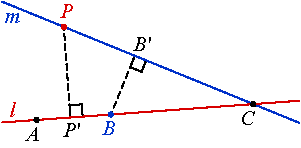
\includegraphics[height=.95in]{main/Sylvester_Gallai_Kelly_proof}
\vskip-8pt
\caption{Construction for the Sylvester-Gallai theorem.}
\label{Fig4-S}
\end{figure}
%
in $\PP^2_\CC$ passes through a third flex; but
such a configuration is not possible in $\PP^2_\RR$. Prove:

\begin{theorem}[Sylvester--Gallai theorem]
In any finite set  $\Gamma \subset \PP^2_\RR$ there are three
noncollinear points unless $\Gamma$ is contained in a line.
\unif
\end{theorem}

Hint (following Leroy Milton Kelly):
\index{Kelly, Leroy Milton}%
We may assume that $\Gamma\subset \RR^2` `$. Choose a pair $P,L$ consisting of a point $P\in\Gamma$ and line $\ell$ containing at least 2 of the points of $\Gamma$, but not $P$, such that the distance from $L$ to $p$ is
minimal among such pairs. If there were at least 3 points of $\Gamma$
on $L$ then, considering
Figure~\ref{Fig4-S},
show that
there is a point of $\Gamma$ and a line $L'$ violating the minimal distance hypothesis.
\end{exercise}

\input header.tex

\chapter{Jacobians}


Up to now, we have been treating line bundles on a curve $C$ individually. It is a fundamental fact, however, that the set of line bundles/linear equivalence classes of divisors of a given degree $d$ on $C$ is naturally parametrized by the points of a variety, called the \emph{Picard variety} and denoted ${\rm Pic}^d(C)$. Many of the deeper results about linear systems on $C$ are expressed in terms of the geometry of this variety, and indeed the simple fact of its existence is the key to proving many theorems about linear systems on curves (see for example Theorem~\ref{g+3 theorem}
below).

In this chapter, we will describe the construction of these varieties, and their relationship with the spaces parametrizing effective divisors of a given degree $d$ on $C$. We then exhibit some of the consequences of these constructions.

\section{Jacobians}

We start with the construction of a classical object, the \emph{Jacobian} $J(C)$ of a curve $C$, via the notion of \emph{abelian integrals}. This necessitates that we work over the complex numbers $\CC$, and it produces a complex manifold rather than an algebraic variety, but has the virtue of being relatively concrete. The Jacobian $J(C)$ is in fact a projective variety, and may be constructed purely algebraically---so that, for example, if the curve $C$ is defined over a given field $K$ then $J(C)$ will be as well. (Indeed, the search for such a construction was one of the driving forces of algebraic geometry in the first half of the 20th century, giving rise ultimately to the notion of abstract algebraic varieties.) We will not do that here, though; the interested reader can find an account in \cite{??s} [Kleiman must have something for this].

The goal of the 19th century mathematicians who first described abelian integrals was simply to make sense of integrals of algebraic functions. Very briefly: in the early development of calculus, mathematicians figured out how to evaluate explicitly integrals such as
$$
\int_{t_0}^t \frac{dx}{\sqrt{x^2+1}}.
$$
To describe the solution in algebrao-geometric terms, the idea was that such integrals could be thought of as path integrals of meromorphic differentials on the Riemann surface associated to the equation $y^2 = x^2+1$. This surface is isomorphic to $\PP^1$, meaning that $x$ and $y$ could be expressed as rational functions of a single variable $z$; making the corresponding change of variables transformed the integral into one of the form
$$
\int_{s_0}^s R(z)dz,
$$
with $R$ a rational function, and such integrals are readily evaluated by the technique of partial fractions.

When they tried to extend this to similar-looking integrals like
$$
\int_{t_0}^t \frac{dx}{\sqrt{x^3+1}},
$$
however, they were stymied. The reason gradually emerged: the problem is that the Riemann surface associated to the equation $y^2 = x^3+1$ is not $\PP^1$, but rather a curve of genus 1. In particular  the integral depended on a choice of path; that is, it was defined only modulo a lattice $\ZZ^2 \subset \CC$. This meant, among other things, that the inverse function would be a doubly periodic meromorphic function on $\CC$, and not an elementary function. This led to the introduction of a host of new special functions, such as the Weierstrass $\sP$-function.

The next step was to try to extend this theory to path integrals of holomorphic differentials on curves of arbitrary genus. One problem is that the dependence of the integral on the choice of path is much worse; the set of homology classes of paths between two points $p_0, p \in C$ is identified with $H_1(C,\ZZ) \cong \ZZ^{2g}$ rather than $\ZZ^2$. The solution to this is to consider the integral of \emph{all} holomorphic differentials on $C$ simultaneously, rather than one at a time.

To express the resulting construction in relatively modern terms, let $C$ be as above a smooth projective curve of genus $g$ over $\CC$, and consider the space $V = H^0(K_C)^*$ of linear functions of the space of holomorphic differentials. Integration over closed loops in $C$ defines a linear function on 1-forms, so that we have a map
$$
H_1(C,\ZZ) \; \to \;  H^0(K_C)^*.
$$
Using fairly basic Hodge theory, we can see that \emph{this map is injective, with image a discrete, cocompact lattice $\Lambda \subset V$}; we define the \emph{Jacobian} $J(C)$ of $C$ to be the quotient
$$
J(C) \; = \; V/\Lambda.
$$
(As we said, $J(C)$ is in fact an abelian variety, though for any of the applications we have in mind here we don't need to know that; it's sufficient to know that $J(C)$ is a complex torus of dimension $g$.) The point of this construction is that for any pair of points $p, q \in C$, the expression $\int_q^p$ describes a linear functional on $H^0(K_C)$, defined up to functionals obtained by integration over closed loops, and thus a point of $J(C)$. Thus, for example, if we fix the point $q$, we get a holomorphic map
$$
\mu \; : \; C \; \to \; J(C).
$$
This is an example of what is called an \emph{Abel-Jacobi map}.

To fully utilize this, we want to extend it from points  to divisors on $C$, and to do this we need to find a space parametrizing effective divisors on $C$. This is readily available: since an effective divisor of degree $d$ on $C$ is an unordered $d$-tuple of points on $C$, with repetitions allowed, it corresponds to a point in the \emph{$d$th symmetric power} $C_d$ of $C$, defined to be the quotient of the ordinary product $C^d$ by the action of the symmetric group $\Sigma_d$ on $d$ letters. This is a smooth, $d$-dimensional projective variety. Having chosen a base point $q \in C$ as above, we get for each $d$ a map
$$
\mu_d \; : \; C_d \; \to \; J(C),
$$
defined by
$$
\mu_d(p_1 + \dots + p_d) \; = \; \sum \int_q^{p_i}.
$$
These are similarly called  Abel-Jacobi maps; when there is no ambiguity about $d$, we will denote them simply by $\mu$.

There is a lot to say about these maps; in the following sections, we'll see a description of their differentials, and show that they are birational onto their images for $d \leq g$ and surjective for $d \geq g$. (These statement in case $d=g$ form the celebrated \emph{Jacobi inversion theorem}.) But before we get into these, we should say what all this has to do with our main concern, the geometry of linear series on curves.

To this point, the discussion in this chapter might seem more at home in an advanced calculus text than in an algebraic geometry book. The connection is made by \emph{Abel's theorem}:

\begin{theorem}
Two divisors $D, D' \in C_d$ on $C$ are linearly equivalent if and only if $\mu(D) = \mu(D')$; in other words, the fibers of $\mu_d$ are exactly the complete linear systems of degree $d$ on $C$.
\end{theorem}

\begin{proof}[Half-proof]
One direction of Abel's theorem---the ``only if" part---is relatively elementary, and that is what we will prove here. (This was in fact the only part proved by Abel; the converse, which is substantially more subtle, was proved by Clebsch. See \cite{} [GH] for a proof.)

To prove the easy half of Abel's theorem, suppose that $D$ and $D'$ are linearly equivalent; that is, $\cO_C(D) \cong \cO_C(D')$. Call this line bundle $\cL$, and suppose that $D$ and $D'$ are the zero divisors of sections $\sigma, \sigma' \in H^0(\cL)$.
Taking linear combinations of $\sigma$ and $\sigma'$, we get a pencil $\{D_\lambda\}_{\lambda \in \PP^1}$ of divisors on $C$, with
$$
D_\lambda \; = \; V(\lambda_0\sigma + \lambda_1\sigma'),
$$
and this corresponds to a regular map $\alpha : \PP^1 \to C_d$. 

Consider now the composition
$$
\phi = \mu \circ \alpha \; : \; \PP^1 \; \to \; J(C).
$$
We observe that, since $J(C)$ is a complex torus, the global holomorphic 1-forms on $J(C)$ generate the cotangent bundle everywhere. But for any 1-form $\omega$ on $J(C)$, the pullback $\phi^*\omega$ is a global holomorphic 1-form on $\PP^1$, and hence identically zero. It follows that the differential $d\phi$ vanishes identically, and hence (since we are blessedly in characteristic 0) that $\phi$ is constant; thus $\mu(D) = \mu(D')$.
\end{proof}

Note that many of the statements about the Abel-Jacobi map made above follow immediately from Abel's theorem. For example, if  $D = p_1+\dots+p_d\in C_d$ is a general point and $d \leq g$, the points $p_i \in C$ are general and so impose independent conditions on $H^0(K_C)$; thus $h^0(K_C(-D)) = g-d$ and by Riemann-Roch $h^0(\cO_C(D)) = 1$. In other words, the fiber of $\mu_d$ containing $D$ consists just of the single point $D$, and so the map $\mu_d$ is birational onto its image. Similarly, if $d \geq g$, we will have $h^0(K_C(-D)) = 0$ and hence $h^0(\cO_C(D)) = d-g+1$; it follows that the fiber of $\mu_d$ through $D$ has dimension $d-g$, and hence that $\mu_d$ is surjective. In particular, when $d=g$ the map $C_g \to J(C)$ is a birational isomorphism; indeed, it was by using this isomorphism that Weil first gave an algebraic construction of $J(C)$.

To illustrate some of the power of Abel's theorem, we will use it to prove a basic result:

\begin{theorem}\label{g+3 theorem}
Let $C$ be a smooth projective curve of genus $g$, and $D \in C_{g+3}$ a general divisor of degree $g+3$ on $C$. Then $D$ is very ample; in particular, every curve of genus $g$ may be embedded in projective space as a curve of degree $g+3$.
\end{theorem}

This is, of course, a substantial improvement over our earlier result (\ref{****}) that every curve of genus $g$ may be embedded in projective space as a curve of degree $2g+1$. It is also sharp: hyperelliptic curves, for example, cannot be embedded in projective space as curves of any degree less than $g+3$. Nonetheless, we will see in Chapter~\ref{****} that we can improve on this: ``most" curves of genus $g$ can in fact be embedded in projective space as curves of degree $d = \lceil 3g/4 \rceil + 3$.

\begin{proof}
As we observed above, since $D$ is general of degree $g+3$ we have $h^0(\cO_C(D)) = 4$. To show that it is very ample, we have to show that
\begin{enumerate}
\item for any point $p \in C$, we have $h^0(\cO_C(D-p)) = 3$ (that is, $|D|$ has no base points, and so defines a regular map $\phi_D : C \to \PP^3$); and
\item for any pair of points $p, q \in C$, we have $h^0(\cO_C(D-p-q)) = 2$.
\end{enumerate}
The second of these assertions immediately implies the first, and this is what we will prove.

To do this, suppose on the contrary that for some pair of points $p, q \in C$ we have $h^0(\cO_C(D-p-q)) \geq 3$. It follows from Riemann-Roch that $h^0(K_C(-D + p + q)) \geq 1$; that is, $K_C -D + p + q$ is linearly equivalent to an effective divisor $E = r_1 + \dots + r_{g-3}$ of degree $g-3$.

Now consider the map
$$
\nu : C_{g-3} \times C_2 \; \to \; J(C)
$$
given by
$$
\nu : (E,F) \; \mapsto \; \mu(K_C) + \mu(E) - \mu(F),
$$
where the $+$ and $-$ on the right refer to the group law on $J(C)$. By what we have just said, and Abel's theorem, our divisor $D$ will fail to be very ample only if there exist effective divisors $F = p+q$ and $E = r_1+\dots+r_{g-3}$ such that $D \sim K_C +E-F$, that is, if
$\mu(D) \in {\rm Im}(\nu)$. But the source $C_{g-3} \times C_2$ of $\nu$ has dimension $g-1$, and so its image in $J(C)$ must be a proper subvariety; since $\mu_{g+3}$ is dominant, the image $\mu(D)$ of a general point $D \in C_{g+3}$ will be a general point of $J(C)$ and so will not lie in ${\rm Im}(\nu)$. It follows that $D$ is very ample, and gives an embedding of $C$ in $\PP^3$ as a curve of degree $g+3$.
\end{proof}

Thus Abel's theorem, which was born out of an effort to evaluate calculus integrals, winds up proving a basic fact in the theory of algebraic curves!

\

\

****A minor issue, but one that's bothering me: we said early on that we don't need to know that $J(C)$ is algebraic; for the present purposes, it's enough to know that $J(C)$ is a  complex torus of dimension $g$. But in that case we do need to know that if $f : X \to Y$ is a holomorphic map of compact complex manifolds with $\dim X < \dim Y$, then $f(X)$ is a proper analytic subvariety of $Y$. Should this bother us?****

trivial change to Jacobians

\section{Picard varieties}

\section{Differential of the Abel-Jacobi map}

In this section we will describe the differential $d\mu$ of the Abel-Jacobi map $\mu : C_d \to J(C)$; this turns out to be pretty straightforward, but yields among other things a sharper form of Abel's theorem.

To start, suppose $D = p_1 + \dots + p_d$ is a divisor consisting of $d$ distinct points on our curve $C$. Since the quotient map $C^d \to C_d$ is unramified at $D$, the tangent space to $C_d$ at the point $D$ is naturally identified with the tangent space to $C^d$ at $(p_1,\dots,p_d)$; that is, the direct sum of the tangent spaces to $C$ at the points $p_i$:
$$
T_D(C_d) = \bigoplus T_{p_i}(C).
$$
On the other hand, the tangent space to $J(C)$ at the image point $\mu(D)$ is simply the vector space $H^0(K_C)^*$ of which $J(C)$ is a quotient (as it is at every point!). The differential $d\mu_D$ is thus a linear map
$$
\bigoplus T_{p_i}(C) \rTo H^0(K_C)^*,
$$
and the transpose of this a linear map
$$
H^0(K_C) \rTo \bigoplus T^*_{p_i}(C).
$$
This last map is easy to describe: since the map $\mu$ is given by 
$$
\mu_d(p_1 + \dots + p_d) \; = \; \sum \int_q^{p_i},
$$
we can simply differentiate under the integral sign to conclude that \emph{the codifferential $d_\mu^*$ is the map}
\begin{align*}
H^0(K_C) &\to \bigoplus T^*_{p_i}(C) \\
\omega &\mapsto (\omega(p_1), \dots, \omega(p_d).
\end{align*}

There is a natural extension of this to the case of non-reduced divisors $D$, that is, divisors with repeated points. We need here a description of the tangent space to $C_d$ at the point $D$, and to this end we have the

\begin{proposition}\label{symmetric product tangent space}
The tangent and cotangent spaces to $C_d$ at the point corresponding to an arbitrary divisor $D = \sum a_ip_i$ are naturally identified with $H^0(\cO_C(D)/\cO_C)$ and $H^0(K_C/K_C(-D))$ respectively.
\end{proposition}

Note that we have a natural pairing between the spaces $H^0(\cO_C(D)/\cO_C)$ and $H^0(K_C/K_C(-D))$, given by sending $(f, \omega)$ to $\sum_i Res_{p_i}(f\omega)$. Note also that the term ``natural" has a precise meaning here: if we let 
$$
\cD = \{ (D, p) \in C_d \times C \; \mid \; p \in D \}
$$
be the universal effective divisor of degree $d$ on $C$, the proposition says that the cotangent sheaf $T^*_{C_d}$ is the direct image $\alpha_*(\beta^*K_C/\beta^*K_C(-\cD))$, where $\alpha$ and $\beta$ are the projections of $C_d \times C$ onto the two factors.

If you wanted to see an argument for Proposition~\ref{symmetric product tangent space} done out in coordinates (you really don't, but if you did) you could find it in [ACGH].

In any event, given Proposition~\ref{symmetric product tangent space}, we can extend our earlier statement to the

\begin{proposition}\label{differential of Abel-Jacobi}
The codifferential $d\mu^*$ of the Abel-Jacobi map is simply the natural restriction map
$$
H^0(K_C) \rTo H^0(K_C/K_C(-D)).
$$
\end{proposition}

Now, note that the codimension of the image of $d\mu^*$---equivalently, the dimension of the kernel of the differential $d\mu$---is by the geometric Riemann-Roch theorem exactly the dimension of the fiber of $C_d$ over the point $\mu(D) \in J(C)$. In other words, the fibers of $\mu$ are smooth, and in particular reduced. Thus we can think of Proposition~\ref{differential of Abel-Jacobi} as a strengthening of the Abel-Clebsch theorem: while Abel and Clebsch show that the fibers of $\mu$ are complete linear series set-theoretically, we see from the above that it is in fact true scheme-theoretically.

\section{Further consequences}

xxx

\input footer.tex



\chapter{Hyperelliptic curves and curves of genus 2 and 3}
\label{genus 2 and 3 chapter}

\section{Hyperelliptic curves}
\label{hyperelliptic}

Recall that a hyperelliptic curve $C$ is a curve of genus $\geq 2$
admitting a map $\pi : C \to \PP^1` `$ of degree 2.
We met hyperelliptic curves in Chapter~\ref{RiemannRochChapter} and proved
that
\index{hyperelliptic curve}%
the canonical
map from $C$ is the composition of $\pi$ with
the embedding of $\PP^1$ in $\PP^{g-1}$ as a rational normal curve,
showing in particular that $\pi$ is unique up to automorphisms of $\PP^1$.

 We used this to show that every special
linear series on a hyperelliptic curve is a sum of a multiple of  the
unique $g^1_2$ plus basepoints. We will begin this chapter with an
explicit construction of hyperelliptic curves and use it to give a
concrete computation of the canonical series, reproving what we did in
Chapter~\ref{RiemannRochChapter}.
Then we will consider the projective embeddings of curves of
genus 2 (which are all hyperelliptic) and genus 3.

There will be a further discussion of hyperelliptic curves in
Chapter~\ref{ScrollsChapter}.

\subsection*{The equation of a hyperelliptic curve}

 Because the degree of the canonical map is  2, each point in $\PP^1$
has either two distinct preimages, or only one; in the latter case,
this point is a
ramification point
\index{ramification point}%
with ramification index 1; that is, the
map is given in terms of local analytic coordinates on $C$ and $\PP^1$
by $z \mapsto z^2` `$. In particular, both the
ramification divisor
\index{ramification divisor}%
and
the
branch divisor
\index{branch divisor}%
(as defined in Chapter~\ref{RiemannRochChapter}) are
reduced. By
Hurwitz's formula
\index{Hurwitz's formula}%
there are exactly $2g+2$ branch points
in $\PP^1` `$. These points determine the curve:

\begin{theorem}
\label{hyperelliptic existence}
There is a unique smooth projective hyperelliptic curve $C$ expressible
\index{hyperelliptic curve!uniqueness}%
as a
$2$-sheeted cover
\index{2-sheeted cover}%
of $\PP^1$ branched over any given set of $2g+2$
distinct points $\{q_{1}, \dots, q_{2g+2}\}$.
\unif
\end{theorem}

\begin{proof}
We
will exhibit
 such a curve,
leaving the proof of uniqueness to Section~\ref{branched covers}.
If the coordinate of the point $q_i \in \PP^1$ is $\lambda_i$,
we take for $C$
the smooth
projective model
\label{projective model}%
of the affine curve
  $$
 \tsty\let\big\Big
C^\circ = \big\{@(x,y) \in \AA^2 \bigm|  y^2 = \prod\limits_{i=1}^{2g+2}
(x - \lambda_i)@\big\}.
$$
Note that we're choosing a coordinate $x$ on $\PP^1$ with the point
$x = \infty$ at infinity not among the $q_i$, so that the preimage of
$\infty \in \PP^1$ is two points $r, s \in C$. Concretely, we see that
as $x \to \infty$, the ratio $y^2/x^{2g+2}$
approaches
$1$, so that
$$
\lim_{x \to \infty} @ \frac{y}{x^{g+1}}  =  \pm 1.
$$
  The two possible values of this limit correspond to the two points
  $r,s \in C$.
\end{proof}

The curve $C$
thus constructed
is \emph{not} simply the closure of the affine curve
$C^\circ \subset \AA^2$ in either $\PP^2$ or $\PP^1 \times \PP^1` `$: as
you can see from a direct examination of the equation, each of these
closures will be singular at the (unique) point at infinity.

To give a smooth projective model of
a
hyperelliptic curve $C$ with
given branch divisor, we divide the $2g+2$ branch points  into two sets
of the
same size,
 $\{q_1,\dots,q_{g+1}\}$ and $\{q_{g+2}, \dots,
q_{2g+2}\}$. We can then take $C$ to be the closure in $\PP^1 \times \PP^1$
of the  locus
  $$
 \tsty\let\big\Big
  \big\{@(x,y) \in \AA^2  \bigm|  y^2\prod\limits_{i=1}^{g+1} (x - \lambda_i)
  = \prod\limits_{i=g+2}^{2g+2} (x - \lambda_i)@\big\};
  $$
  in projective coordinates, this is
   $$
 \tsty\let\big\Big
  C  =  \big\{@((X_{0},X_{1}), (Y_{0},Y_{1})) \in \PP^1 \times
  \PP^1  \bigm|  Y_1^2\prod\limits_{i=1}^{g+1} (X_1 - \lambda_iX_0) =
  Y_0^2\prod\limits_{i=g+2}^{2g+2} (X_1 - \lambda_iX_0)@\big\}.
  $$
To see that $C \subset \PP^1 \times \PP^1$ is smooth we note that it is a
curve of
bidegree
\index{bidegree}%
$(2,g@{+}@1)$ in $\PP^1 \times \PP^1` `$, and the formula for
the genus of a curve in $\PP^1 \times \PP^1$ derived in
Example~\ref{Div of quadric} tells us that such a curve has
arithmetic genus $g$, and thus no singular points.

From this model, we deduce:

\begin{corollary}
\label{relation on ramification points}
If $C$ is a hyperelliptic curve  and $p_1,\dots,p_{2g+2} \in C$ are the
ramification points of the unique degree $2$ map $C \to \PP^1` `$, then for any
division of $\{1,\dots,2g+2\}$ into two sets $A,B$ of cardinality $g+1$,
$$
\sum_{i\in A} p_{i}   \sim  \sum_{i\in B}p_{i}.
$$
\end{corollary}

\begin{proof}
The abstract curve $C\subset \PP^{1}\times \PP^{1}$ above
is independent of the
choice of $A$ and $B$,
since in any case the projection to the
first factor
is ramified at the same set $p_{1}, \dots, p_{2g+2}$. Given the
representation above, the sets
$\{p_i\mid i\in A\}$ and  $\{p_i\mid i\in B\}$
are
preimages of $(0,1)$ and
$(1,0)$ in the second factor.
\end{proof}

 The map $\iota : C \to C$ that exchanges the two points in each reduced
 fiber of the map $C \to \PP^1$ and fixes the ramification points is
 algebraic: in terms of the last representation of $C$, it is given by
 $((X_0,X_1), (Y_0,Y_1)) \mapsto  ((X_0,X_1), (Y_0,-Y_1)) $. The map
\index{hyperelliptic involution}%
\index{involution!hyperelliptic}%
 $\iota$ is called the \emph{hyperelliptic involution} on $C$.

\subsection*{Differentials on a hyperelliptic curve}
%  \label{hyperelliptic differentials}

We can give a pleasantly concrete \null description of the differentials,
and thus the
canonical linear system,
\index{canonical linear series}%
on a hyperelliptic curve $C$
by working with the affine model $C^\circ = V(f) \subset \AA^2` `$, where
$$
f(x,y) = y^2 - \prod_{i=1}^{2g+2} (x - \lambda_i).
$$
We will again denote the two points at infinity (that is, the two points
of $C \setminus C^\circ$) by $r$ and $s$; for convenience, we'll denote
the divisor $r+s$ by $D$. We write $\pi:C \to \PP^1$ for the morphism
that, on $C^\circ$, sends $(x,y) \in C$ to $x$.

We can construct a differential form on $C$ by following the proof of
Hurwitz's theorem
\index{Hurwitz's theorem}%
in
Chapter~\ref{RiemannRochChapter}.
Let $dx$ denote the usual differential on $\PP^1$ having a double
pole at infinity, and consider $\pi^*dx$ on $C$.  The function $x$ is
regular on $C^\circ$, and is a local parameter over points other than
the $\lambda_i$; from the local description of the map $\pi$, we see that
$\pi^*dx$ is regular on $C^\circ$  with simple zeros at the ramification
points $q_i = (\lambda_i, 0)$. Since $dx$ has a double pole at the
point at $\infty\in \PP^1$ and $\pi$ is a local isomorphism near $r$
and $s$, the differential $\pi^*dx$ has double poles at the points $r$
and $s$. Thus the canonical
divisor of $C$ is
$$
 K_C \sim (dx) \sim R - 2D,
$$
where $R$ denotes the ramification divisor, in this case the sum of the
ramification points.

How can we find differentials that are regular everywhere on $C$? If we
divide $dx$ by $x^2$ (or any quadratic polynomial in $x$) to kill the
poles we  introduce new poles in the finite part $C^\circ$ of $C$.

Instead, we want to multiply $dx$ by a rational function with zeros
at $r$ and $s$, but whose poles occur only at the points where $dx$
has zeroes\emdash that is, the points $\lambda_i$.  A natural choice is the
reciprocal of the partial derivative $f_y \colonequals  \partial f/ \partial y =
2y$, which vanishes at the points $q_i$, and has  a pole of order $g+1$
at each of the points $r$ and $s$ (reason: $y/x^{g+1}$ approaches $\pm
1$ as $x$ goes to infinity, and $x$ has a pole of order 1 at $\infty\in
\PP^{1}$ and thus also at each of $r,s$). In other words, as long as $g
\geq 1$, the differential
$$
\omega = \pi^*\left(\frac{dx}{f_y}\right)
$$
is regular, with divisor
$$
(\omega) = (g-1)@r + (g-1)@s = (g-1)@D.
$$
The remaining regular differentials on $C$ are now easy to find: Since
$x$ has only a simple pole
at the two points at infinity we can  multiply $\omega$ by any $x^k$ with
$k = 0, 1, \dots, g-1$.
This gives us $g$ differentials
$$
\omega, x\omega, \dots, x^{g-1}\omega
$$
that are independent, and so form a basis for $H^0(K_C)$.

With this description of the differentials, we can see clearly why the
canonical map of a hyperelliptic curves is degree 2 onto a rational
normal curve, as proved in Chapter~\ref{RiemannRochChapter}:
the relations on
$
\omega, x\omega, \dots, x^{g-1}\omega
$
are the relations on $x^i` `$, and we see that the canonical image is the
rational normal curve
\index{rational normal curve}%
 of degree $g-1$.

\section{Branched covers with specified branching}
\label{branched covers}

Given a curve $B$ and points
$\thinmuskip=3mu plus 2mu p_1,\dots,p_b$ in $B$,
what are the branched covers $\pi :\nobreak C \to\nobreak B$
of degree $d$ with specified branching over each of the points $p_i$,
up to isomorphism over $B$?
We will reduce this question to the classification of topological
covering spaces of the complement $U = B \setminus \Delta$; we will
then use properties of the fundamental group of $U$ to enumerate such
covering spaces. We will prove the uniqueness of hyperelliptic curves with specified branch points
at the end of this section as a special case of a general analysis of branched covers.

\begin{theorem}
 Let $B$ be a smooth curve, let $\Delta\subset B$ be a finite set of
 points, and let $U \colonequals  B\setminus \Delta$.
If $\pi^\circ : V \to U$ is a topological covering space then $V$ may
be given the structure of a
Riemann surface
\index{Riemann surface}%
in a unique way so that
the map $\pi^\circ$ is holomorphic; and $V$ may be compactified to a
compact Riemann surface $C$ in a unique way such that the map $\pi^\circ$
extends to a holomorphic map $\pi : C \to B$.
\unif
\end{theorem}

\begin{proof}
The space $V$ inherits the structure of a complex manifold from $U$
because if $D \subset U$ is any simply connected coordinate chart,
then the preimage $({\pi^\circ})^{-1}(D)$ is a disjoint union of $d$
copies of $D$, and we may use them as coordinate charts on $V` `$.

To compactify $V$ we observe that if $D^* = \{ z \in \CC \mid 0 < |z|
< 1 \}$ is a punctured disc, then
the map
$z \mapsto z^n$ on the unit disk
restricts to a connected $n$-fold covering
space $D^*\to D^*` `$.
Since $\pi_1(D^*) = \ZZ$, any connected covering space $E$ of degree $n$
is homeomorphic to this one
by a homeomorphism inducing the identity on the target of $\pi$.
If we  define a holomorphic structure on $E$ by pulling back the one on
$D$, then
this homeomorphism is biholomorphic.

Thus if $D_i$ is a small neighborhood of the point $p_i \in B$
biholomorphic to a disc, then the preimage  in $V$ of the punctured
disc $D_i^* \colonequals  D_i \cap U$ is a disjoint union of punctured discs
$E_{i,j}^{*}$. The maps $E^{*}_{i,j} \to D_{i}^{*}$
are homeomorphic to the maps $z\mapsto z^{n_{i,j}}$
of the punctured unit disc
for some
$n_{i,j}$. Because of the way the holomorphic structure
of $V$ is defined, the maps
$E^{*}_{i,j} \to D_{i}^{*}$
are actually
holomorphic. Thus they extend holomorphically
to maps of the full disks $E_{i,j}\to D_{i}$ and $V@\cup@ \bigcup` E_{i,j}$
is a compact Riemann surface in a unique way.
\end{proof}

The problem of classifying smooth curves $C$ that have a map $\pi : C \to B$
of~degree $d$ thus becomes one of classifying covering spaces of $U$.
\index{covering space}%

\subsection*{Branched covers of $\PP^1$}

We continue with the notation $U = B\setminus \Delta$, now supposing
\index{branched cover!of $\PP\sp1$}%
that $B = \PP^1_\CC$, the Riemann sphere. Again, let $\pi:V\to U$ be a
covering space.

Choose a basepoint $p_0 \in U$, and draw simple, nonintersecting arcs
$\gamma_i$ joining $p_0$ to $p_i$ in $U$. If $\Sigma$ is the complement
of the union of these arcs in the sphere, then the preimage of $\Sigma$
in $V$ will be the disjoint union of $d$ copies of~$\Sigma$, called the
\index{sheet!of a cover}%
\emph{sheets} of the cover; label these $\Sigma_1,\dots,\Sigma_d$.

Given $U$, elementary homotopy theory asserts the existence of a bijection
between coverings $V \to U$ of $U$ of degree $d$ (up to homeomorphisms
of $V$ fixing~$U$) and group
homomorphisms
   $$
 M:  \pi_1(U, p_0) \to S_d,
   $$
to the symmetric group on $d$ letters, up to inner automorphisms of
\index{symmetric group}%
\index{inner automorphism}%
$S_{d}$. The map $M$ is called the \emph{monodromy} of the covering:
given $V \to U$
and a labeling of the $d$ sheets of $V$ over the point
$p_0$, the value of $M$ at a loop  $\beta$ in $U$ based at $p_0$
is the
permutation of the points of $\pi^{-1}(p_0)$ given by sending a point
$q \in \pi^{-1}(p_0)$ to the endpoint of the unique lift of $\beta$
starting at $q$. A permutation $\sigma$ of the labels  of the sheets
leads to a map $M'$ equal to the composition of $M$ with conjugation
by $\sigma$.

A convenient set of generators of $ \pi_1(U, p_0)$ is the set of paths
$\beta_i$ indicated in Figure~\ref{pi 1 generators}: starting at $p_0$,
going out along the arc $\gamma_i$ until just short of $p_i$, going
once around $p_i$ and then going back to $p_0$ along the same path
$\gamma_i$. The fundamental group
\index{fundamental group}%
\index{free group}%
 of $U$ is the free group generated
by the paths $\beta_1,\dots \beta_b$ \null modulo the relation $\prod_{i=1}^b
\beta_i = 1$
which comes from the fact that the sphere minus the part enclosed by
the paths $\beta_i$ is
contractible.
{\meshing\par}

\begin{figure}
\centerline{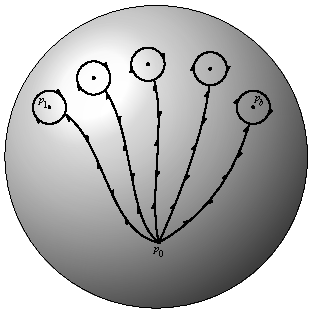
\includegraphics[height=1.8in]{main/Fig05-1}}
\vskip-6pt
 \caption{Generators for the fundamental group of a multiply punctured
 sphere.}
 \label{pi 1 generators}
\end{figure}

Given a degree $d$ covering space $V$ and a labeling of the $d$ sheets
over the point $p_0$, let $\tau_i$ be the permutation of $\{1,2,\dots,d\}$
corresponding to the path $\beta_i$. The space $V$ is connected if and
only if the $\tau_{i}$ generate a transitive subgroup of~$S_{d}$. The
case $d=2$ is illustrated in Figure~\ref{square root function graph}.

If we start from a map of Riemann surfaces $C\to \PP^{1}$ that is
 simply branched, and take $V$ to be the complement of the set of
 branch points,
 then each $\tau_i$ is a transposition.

\begin{figure}
\vskip1pt
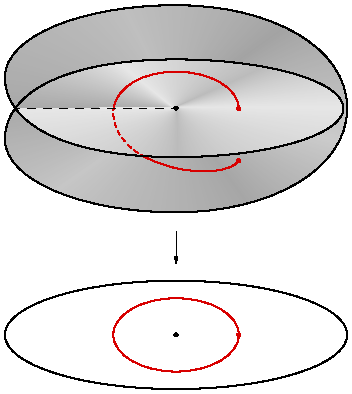
\includegraphics[height=2.1in,trim=0 2 0 0,clip]{main/Fig05-2-good}
\vskip-3pt
\caption{Local picture of a simple branch point $z \mapsto z^2` `$.
}
\index{simple branch point}%
\index{branch point!simple}%
\label{square root function graph}
\end{figure}

Summarizing we have proven:
   \begin{lemma}
   \label{branched cover classification}
   Let $p_1,\dots, p_b \in \PP^1$ be any $b$
distinct
points. There is a
   natural bijection between
   \begin{enumerate}
   \item the set of  simply branched covers $\pi : C \to \PP^1$ of
   degree $d$, branched over the points $p_i$, up to isomorphism over
   $\PP^1$; and
   \item the set of $b$-tuples of transpositions $\tau_1, \dots, \tau_b
   \in S_d$ such that
\smallbreak
\begin{enumerate}
 \item $\prod \tau_i$ is the identity, and
 \item $\tau_1, \dots,
   \tau_b$ generate a transitive subgroup of $S_d$,
\end{enumerate}
\smallbreak
\noindent modulo simultaneous
   conjugation by $S_d$.
   \qed
   \end{enumerate}
\let\qed\relax
   \end{lemma}

\begingroup \def\,{\kern1pt}
\begin{proof}[Proof \,of \,the \,uniqueness \,statement \,in
Theorem~\ref{hyperelliptic existence}.]
In the case of double covers of $\PP^1$ that is relevant to hyperelliptic curves, we note that
there is only one transposition in $S_2$. Thus there is a unique double
cover of $\PP^1$ with given branch points $p_1,\dots,p_b$. (The product
condition shows again that the number of branch points must be even.) This
completes the proof of Theorem~\ref{hyperelliptic existence}.
\emergencystretch1pt
\end{proof}
\endgroup

\begin{example}
In contrast to the situation of double covers of $\PP^1$, there are generally many
branched covers of specified degree  greater than 2 or with given branch points
and given conjugacy classes of the local monodromy.
The number of these is called
the \emph{Hurwitz number}
\index{Hurwitz number}%
of the configuration, and its computation in
general is the subject of a large and active literature; see for example
\cite{ELSV}.

To illustrate this, we can use Lemma~\ref{branched cover classification} to count the number of
degree 3 branched covers
\index{3-sheeted cover}%
$C \to \PP^1$ with given simple branch points, using that fact that every
odd permutation $\tau \in S_3$ is a transposition. Thus if $b$ is even
and  $\tau_1,\dots,\tau_{b-1} \in S_3$ are arbitrary transpositions,
then the product
$\tau_1\cdot \cdots\cdot \tau_{b-1}$ is also a
 transposition. It follows that the number of ordered $b$-tuples of
 transpositions $\tau_1,\dots,\tau_{b} \in S_3$ with $\prod \tau_i$
 equal to the identity is $3^{b-1}$. The requirement that the group
 generated by the $\tau_i$ is transitive eliminates just the three
 cases where all the $\tau_i$ are equal. The group $S_3$ acts on the
 set of $b$-tuples of permutations without stabilizing any $b$-tuple,
 so every cover corresponds to exactly 6 sequences
  $\tau_1,\dots,\tau_b$. In sum, the number of simply branched
  3-sheeted covers of $\PP^1$ with specified branch points
  $q_1,\dots,q_b \in \PP^1$ is
$$
\frac{3^{b-1} - 3}{6} \; = \; \frac{3^{b-2} - 1}{2}.
$$
One can use a similar strategy to count covers in other cases, when the
target has higher genus and/or the degree of the covering is larger,
but the combinatorics becomes more complicated.
\end{example}

\section{Curves of genus 2}
\label{genus 2 section}

Since  curves of genus 2 are hyperelliptic, everything we said above
applies to them; in particular, the canonical map $\phi_K : C \to \PP^1$
on a
curve of genus 2
\index{genus 2!curve, maps to $\PP\sp1$}%
 is the expression of $C$ as a double cover of
$\PP^1` `$, simply branched over 6 points in~$\PP^1` `$, which are unique up
to automorphisms of $\PP^1` `$.

In this section, we'll consider other maps from hyperelliptic curves $C$
to projective space, starting with maps $C \to \PP^1` `$.
See for example \cite{transcanonical} for a treatment of certain
embeddings of hyperelliptic curves of all genera.

\subsection*{Maps of $C$ to $\PP^1$}

The curve $C$ has a unique degree 2 morphism to $\PP^1$  associated
to the canonical system $|K_C|$. But there are many other morphisms to
$\PP^1` `$. For example, there is a 2-parameter
family of maps of degree 3:

 Let $\sL$ be an invertible sheaf of degree 3 on $C$. Since $3 > 2g-2$,
 the
Riemann--Roch theorem
\index{Riemann--Roch theorem}%
 tells us immediately that $h^0(\sL) = 2$, and
 there are two possibilities:

\begin{enumerate}
\item If the linear system $|\sL|$ has a basepoint $p \in C$,
then $h^0(\sL(-p)) = 2$, and hence $\sL$ must be of the form $\sL =
K_C(p)$. Conversely, if $\sL = K_C(p)$, then $h^0(\sL(-p)) = h^0(\sL)$, which
is to say $p$ is a basepoint of $|\sL|$. There is a 1-parameter family of
such $\sL$.

\item If $\sL$ is not of the form $\sL = K_C(p)$, then $|\sL|$ does not have
\label{genus 2 pencil} % used for page number
a basepoint, and so defines a degree 3 map $\phi_\sL : C \to \PP^1` `$.
\end{enumerate}

Since the variety $\Pic_3(C)$ has dimension $g= 2$ the general invertible
sheaf of degree 3 is of the second kind, and this gives a 2-parameter
family of such maps.

There are plenty of higher-degree maps as well: an invertible sheaf of
degree $d \geq 4 = 2g$ is basepoint free, and gives a map to $\PP^{d-2}$,
from which we can project in many ways
to $\PP^1` `$.

\subsection*{Maps of $C$ to $\PP^2$}
Next consider maps of a curve $C$ of genus 2 to the plane. By the Riemann--Roch
\index{genus 2!curve, maps to $\PP^2$}%
theorem, an invertible sheaf $\sL$ of degree 4 on $C$
has
$h^0(\sL)
= 3$ and is basepoint free by Corollary~\ref{degree 2g+1 embedding}, so
the linear system $|\sL|$  gives a morphism $\phi_\sL : C \to \PP^2` `$. The
invertible sheaf $\sL\otimes \omega_C^{-1}$ is either
$\omega_C$ or nonspecial; in either case, by the Riemann--Roch theorem,
it has at least one section,
so we may write $\sL\otimes \omega_C^{-1} = \sO_C(p+q)$ for some points
$p,q$. There are two possibilities:

\begin{enumerate}
\item If $p+q =  K_C$, then $\sL = \omega_C^2` `$. Since
the elements of $H^0(\omega_C)$ may be written as $\omega, x\omega$,
the map
$$
\Sym^2 H^0(\omega_C) \to H^0(\sL)
$$
 is injective, and since both sides are 3-dimensional vector spaces,
 they are equal. In other words, every divisor $D \sim 2K_C$ is the sum
 of two divisors $D_1, D_2 \in |K_C|$. We conclude that the map $\phi_\sL$
 is the composition of the canonical map $\phi_K : C \to \PP^1$ with the
Veronese embedding
\index{Veronese!map}%
 $\nu_2 : \PP^1 \to \PP^2$ of $\PP^1$ as a conic in
 the plane and the map $\phi_\sL$ is generically 2-to-1 onto the conic.

\item
\label{p+q not g12}
If $p+q \neq  K_C$  then $h^0(p+q) = 1$, so the pair $p,q$ is
unique. Furthermore,
 $h^0(\sL-p) = 2 =  h^0(\sL(-p-q))$ so
 $H^0(\sL(-p)) = H^0(\sL(-q))$ and $\phi_\sL(p) = \phi_\sL(q)$.
By the genus formula, the
$\delta$ invariant
\index{delta@$\delta$ invariant}%
of this point must be 1. By
Exercise~\ref{delta=1 characterization}
 this is a
node
\index{node!on quartic}%
(if $p\neq q$) or
cusp
\index{cusp!on quartic}%
\index{quartic!with a node or cusp}%
(if $p=q$).
\end{enumerate}

Thus  for $\sL$ in an open subset of $\Pic_4(C)$ the image is a quartic
with a node; for a one-dimensional locus in $\Pic_4(C)$, the image is
a quartic with a cusp; and for one point in $\Pic_4(C)$ the image is
a conic.

\subsection*{Embeddings in $\PP^3$}

By Corollary~\ref{degree 2g+1 embedding} any invertible sheaf $\sL$ of
\index{genus 2!curve, embeddings in $\PP^3$}%
\index{quintic!of genus 2}%
degree 5 is very ample.
Write $\phi_\sL : C \to \PP^3$
for the map given by the complete linear
system $|\sL|$. Since $\phi_\sL$ is an embedding, we'll also denote the
image $\phi_\sL(C) \subset \PP^3$ by $C$ and write $\cO_C(1)$ for $\sL$.

What degree surfaces in $\PP^3$ contain the curve $C$? We start with
degree 2, and consider the restriction map
$$
H^0(\cO_{\PP^3}(2)) \to H^0(\cO_C(2)) = H^0(\sL^2).
$$
The space on the left has dimension 10; by the
Riemann--Roch theorem
\index{Riemann--Roch theorem}%
we have $h^0(\sL^2) = 2\cdot5 - 2 + 1 = 9$. It follows that $C$ lies
on a quadric surface $Q$. Since $C$ is not contained in a plane or a
union of planes, any quadric containing $C$ is irreducible; if there
were more than one such,
B\'ezout's theorem
\index{Bezout@B\'ezout's theorem}%
 would imply that $\deg C
\leq 4$. Thus $Q$ is unique.

We might ask at this point: is $Q$ smooth or a quadric cone? The answer
depends on the choice of invertible sheaf $\sL$.

\begin{proposition}
\label{genus 2 embedding}
Let $C \subset \PP^3$ be a smooth curve of degree $5$ and genus $2$, and
set $\sL = \sO_C(1)$. The unique quadric $Q$ containing $C$
  is singular if and only if
$$
\sL \cong K^2(p)
$$
for some point $p \in C$; in this case, the point $p$ maps to the vertex
of $Q$.
\end{proposition}

\begin{proof}

Suppose first that
$\sL \cong K^2(p)$ for some $p \in
C$. Then $\sL(-p) \cong K^2` `$, so that the map $\pi : C \to \PP^2$ given
by projection from $p$ is the map $\phi_{K^2} : C \to \PP^2$ given by
the square of the canonical sheaf. As we have seen, the map $\phi_{K^2}$
is two-to-one onto a conic $E \subset \PP^2` `$, so that the curve $C$
lies on the cone $Q$ over $E$ with vertex $p$, and this is the unique
quadric surface containing $C$.

On the other hand, if $\sL$ is not of the form $K^2(p)$, then we can write
$$
\sL = K \otimes \sM,
$$
where by hypothesis $\sM$ is not of the form $K(p)$.
We are in case (2) at the bottom of the previous page; that is,
the pencil $|\sM|$ gives a
degree 3 map $C \to \PP^1` `$.

This gives us a way of factoring the map $\phi_\sL : C \to \PP^3` `$: we
have maps $\phi_K : C \to \PP^1$ of degree 2 and $\phi_\sM : C \to \PP^1$
of degree 3, and we can compose their product with the
Segre embedding
\index{Segre embedding}%
$\sigma : \PP^1 \times \PP^1 \to \PP^3$:
$$
C\ruuuto {\hskip0.9em\phi_K \times \phi_\sM}\hskip0.7em
\PP^1 \times \PP^1  \ruto {\ \sigma}  \PP^3.
$$

This description of the map $\phi_\sL$  shows  that \emph{$C$ is a
curve of type $(2,3)$
\index{curve!of type $(2,3)$}%
on a smooth quadric $Q \subset \PP^3$}, completing the
proof of Proposition~\ref{genus 2 embedding}.
\end{proof}

 The variety $\Pic_5(C)$ has dimension 2, while the sheaves
$K^2(p)$ form a one-dimensional subfamily.
Thus for a general invertible sheaf $\sL\in \Pic_5(C)$
the unique quadric $Q$ containing $\phi_\sL(C)$ is smooth.

\subsubsection*{The ideal of a quintic space curve of genus 2}
\label{genus 2 quintic}

Continuing the discussion above, let $C\subset \PP^3$ be a smooth quintic curve of genus 2.
To describe a minimal set of generators of the homogeneous ideal
$I(C) \subset \CC[x_0, x_1, x_2, x_3]$ we look at the
restriction map
$$
H^0(\cO_{\PP^3}(3)) \to H^0(\cO_C(3)).
$$
Since the dimensions of these spaces are 20 and $15-2+1 = 14$
respectively, we see that the vector space of cubics vanishing on $C$
has dimension at least 6.
The subspace of cubics divisible by $Q$ has dimension 4. It follows
that there are at least two cubics vanishing on $C$ that are linearly
independent modulo those vanishing on $Q$.

We can identify these cubics geometrically. Suppose first that $Q$
is smooth, so that $C$ is a curve of type $(2,3)$ on $Q$. In that
case, if $L \subset Q$ is any line of the first ruling, the sum $C+L$
is the complete intersection of $Q$ with a cubic $S_L$, unique modulo
the ideal of $Q$; conversely, if $S$ is any cubic containing $C$ but
not containing $Q$, the intersection $S \cap Q$ will be the union of
$C$ and a line $L$ of the first ruling; thus $S = S_L$
modulo $I(Q)$.
A
similar argument applies in case $Q$ is a cone, and $L$ is any line of
the (unique) ruling of $Q$. In Exercise~\ref{ideal of genus 2 degree 5}
you may show that there are no more cubics containing $C$.

\subsection*{The dimension of the family of genus 2 curves}

Each of the types of maps that we described from a curve $C$ of genus
\index{genus 2!dimension of space of curves}%
2 to projective space suggests
a way to compute the dimension of the family of genus 2 curves, and
indeed, as we will explain in Chapter~\ref{CurvesModuliChapter}, there
is a moduli space of this dimension.

First,  every curve of genus 2 is uniquely expressible as a double
cover of $\PP^1$ branched at six points, modulo the group $\PGL_2$ of
automorphisms of $\PP^1` `$. The space of such double covers has dimension 6,
\index{PGL@$\PGL_2$}%
and $\dim\PGL_2 = 3$, and since the group acts with finite stabilizers
this gives a family of dimension $6-3 = 3$.

Also, each curve  of genus 2 is expressible as a 3-sheeted cover of
$\PP^1$ (with eight branch points) in a 2-dimensional family of ways. As
we saw in Section \ref{branched covers}, such a triple cover is determined
up to a finite number of choices by its branch divisor, so the space of
such triple covers has dimension 8; modulo $\PGL_2$ it has dimension 5, and
\index{3-sheeted cover}%
since every curve is expressible as a triple cover in a two-dimensional
family of ways, we arrive again at a family of dimension $ 5-2 = 3$.

We've also seen that each curve of genus 2 can be realized as (the
normalization of) a plane quartic  with a node in a 2-dimensional family
\index{quartic!with a node or cusp}%
of ways. The space of plane quartics has dimension 14; the family
of those with a node has codimension one
\label{nodal plane quartics}
(Proposition~\ref{local severi geometry})
and hence dimension 13. Since  the automorphism group
\index{PGL@$\PGL_3$}%
$\PGL_3$
of $\PP^2$ has dimension 8, this suggests that the family of nodal
plane quartics modulo $\PGL_3$ has dimension 5. Finally, since every
curve of genus 2 corresponds to a 2-parameter family of such curves,
this again suggests a family of dimension $ 5-2=3$.

Finally, a curve of genus 2 may be realized as a quintic curve in $\PP^3$
in a two-parameter family of ways. To count the dimension of the family
of such curves, note that each one lies on a unique quadric $Q$. We can
assume for this purpose that $Q$ is smooth, since the singular quadrics
and curves on them occur in codimension 1. The curve $C$ is of type
$(2,3)$ on $Q$. Thus to specify such a curve we have to specify $Q$
(9 parameters) and then a bihomogeneous polynomial of bidegree $(2,3)$
on $Q \cong \PP^1 \times \PP^1$ up to scalars; these have $3\cdot 4 - 1 =
11$ parameters. Thus there is a 20-dimensional family of such divisors;
modulo the automorphism group $\PGL_4$ of $\PP^3` `$, this is a 5-dimensional
family. Again, every abstract curve $C$ of genus 2 corresponds to a
2-parameter family of these curves modulo $\PGL_4$, so once more this
suggests a family of dimension $ 5 - 2 = 3$.

\section{Curves of genus 3}

Let $C$ be a smooth projective curve of genus 3. Since we have already
discussed hyperelliptic curves,
we will assume  that $C$ is not hyperelliptic. By
Theorem~\ref{canonical series is very ample}, the canonical map
$\phi_K : C \to \PP^2$ embeds $C$ as a smooth plane quartic curve.
\index{quartic curve!smooth plane}%
Conversely, by Proposition~\ref{adjunction} any smooth plane curve of
degree 4 has genus 3 and is embedded by the complete canonical series.

Since the space of plane quartic curves is 14-dimensional and
$\PGL(3)$ has dimension 8,
this suggests that
there is a 6-dimensional family of curves of genus 3, and in
Chapter~\ref{CurvesModuliChapter}
we will see that
this is indeed the case.
%there is indeed a 6-dimensional moduli space.

\subsection*{Other representations of a curve of genus 3}
\label{other genus 3}
Since we have assumed that $C$ is not hyperelliptic there is no degree 2
cover of $\PP^1` `$. On the other hand, there are degree 3 covers: if $\sL \in
\Pic_3(C)$ is an invertible sheaf of degree 3 then, by the
\index{Riemann--Roch}%
Riemann--Roch theorem, we have
$$
h^0(\sL) =
\begin{tcases}
2 &\text{if $\sL \cong K-p$ for some point $p \in C$,} \\
1 &\text{otherwise.}
\end{tcases}
$$
There is thus a 1-dimensional family of representations of $C$ as a
3-sheeted cover of $\PP^1` `$. These are  visible directly from the canonical
model: a degree 3 map $\phi_{K-p} : C \to \PP^1$ is the composition of
the canonical embedding $\phi_K : C \to \PP^2$ with a projection from $p$,
as illustrated in Figure~\ref{g13 on quartic}.

\begin{figure}
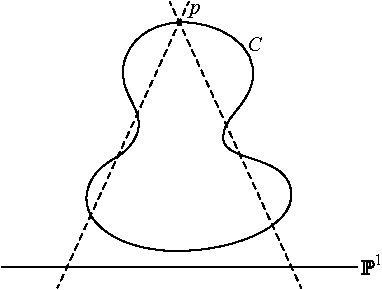
\includegraphics[height=1.7in,trim=0 0 15 0,clip]{main/Fig05-3}%
\llap{\raise12pt\hbox{$\ssty\PP^1$}}
 \caption{Expression of a plane quartic $C$ of genus 3 as a 3-sheeted
\index{3-sheeted cover}%
 cover of $\PP^1$ by projecting the canonical model from a point on it.}
 \label{g13 on quartic}
\end{figure}

There are other representations of $C$ as the normalization of a plane
curve. By
Clifford's theorem
\index{Clifford's theorem}%
 $C$ has no $g^2_3$, and the canonical system
is the only $g^2_4$, but there are plenty of models as plane
quintic curves:
\index{quintic curve!models}%
by Proposition~\ref{very ample}, if $\sL$ is any invertible sheaf
of degree 5, the linear system $|\sL|$ will be a basepoint free $g^2_5$
as long as $L$ is not of the form $K+p$, so that $\phi_\sL$ maps $C$
birationally
\index{birationally}%
onto a
plane quintic curve
\index{plane quintic}%
$C_0 \subset \PP^2` `$. These can
also be described geometrically in terms of the canonical model: any
such invertible sheaf $\sL$ is of the form $2K-p-q-r$ for some trio of
points $p, q, r \in C$ that are not collinear in the
canonical model,
\index{canonical model}%
and we see  that $C_0$ is obtained from the canonical model of $C$ by
applying a
Cremona transform
\index{Cremona transformation}%
with respect to the points $p, q$ and $r$,
that is, by applying the birational transformation
of the plane defined by the linear series of conics through $p,q,r$.

Proposition~\ref{very ample} implies that a divisor $D$ of degree 6 is
very ample if and only if it is not of the form $K+p+q$ for any $p, q
\in C$ and since the family of invertible sheaves on $C$ has dimension 3,
we see that a general invertible sheaf of degree 6 is very ample (indeed,
this is a simple case of Theorem~\ref{g+3 theorem}).

If $C\subset \PP^3$ is a curve of genus 3 embedded as a curve of degree
6, then $C$ cannot lie on a singular quadric since by
Example~\ref{Div of quadric} it would
have to be a complete intersection of the quadric with a cubic, and then
such a curve has genus 4. If $C$ lies on a smooth quadric
in class $(a,b)$ then $a$ or $b$ would be 2, so $C$ would be
hyperelliptic, and conversely any curve in class $(2,4)$
is a hyperelliptic curve of genus 3, degree 6.

Thus if $C$ is not hyperelliptic, then $C$ does not lie on a quadric
surface. We have $h^0(\sO_{\PP^3}(3)) = 20$ while, by the Riemann--Roch
formula, $h^0(\sO_C(3)) = 18-3+1= 16$, so $C$ lies on (at least) 4
independent cubics. Each of these cubics must be irreducible, so any
two of them
intersect in a curve of degree 9 containing $C$ and another component
or components $D$ of degree totaling 3. By
Bertini's theorem
\index{Bertini's theorem}%
if we choose two \emph{general} cubics containing $C$, then each of the
components of $D$ will be smooth. We shall see in
Theorem~\ref{liaison genus formula-first version}
that the arithmetic genus of $D$ must be 0;
thus $D$ must be a
twisted cubic
\index{twisted cubic}%
 curve. The ideal of the twisted cubic
is generated by the $2\times 2$ minors of a matrix of the form
$$
\begin{pmatrix}
 \ell_0& \ell_1&\ell_2\\
 \ell_1& \ell_2&\ell_3\\
\end{pmatrix}
$$
where the $\ell_i$ are linear forms,
and it follows that the two cubics can be written as the two $3\times 3$
minors involving the first two rows of  a matrix of the form
$$
\begin{pmatrix}
\label{hilbert-burch matrix}
 \ell_0& \ell_1&\ell_2\\
 \ell_1& \ell_2&\ell_3\\
\ell_4& \ell_5&\ell_6\\
 \ell_7& \ell_8&\ell_9\\
\end{pmatrix}
$$
where $\ell_4,\dots,\ell_9$ are linear forms as well.
From the
Hilbert--Burch theorem
\index{Hilbert--Burch theorem}%
(Corollary~\ref{Hilbert-Burch}) one can
show that the ideal of $C$ is generated by the four $3\times 3$ minors
of this matrix, whose columns generate
the
syzygies
\index{syzygy}%
of the ideal of the curve.

\section{Theta characteristics}

In this section we sketch the algebraic theory of theta characteristics,
\index{theta characteristic}%
starting with the case of curves of genus 3.

Suppose that $C \subset \PP^2$ is a smooth plane curve. A \emph{bitangent}
\index{bitangent}%
to $C$ is a line $L \subset \PP^2$ that is either tangent to $C$ at
two distinct points, or has contact of order $\geq 4$ with $C$ at a
point. Alternatively, we can say that a bitangent  corresponds to an
effective divisor of degree 2 on $C$ such that $2D$ is contained in the
intersection of $C$ with a line $L \subset \PP^2` `$.

A naive dimension count suggests that a smooth plane curve should have
a finite number of bitangents (it's one condition on a line $L \in
(\PP^2)^*$
to be tangent to $C$, so it should be two conditions for
it to be bitangent). Indeed, this is the case; by
B\'ezout's theorem
\index{Bezout@B\'ezout's theorem}%
a
conic or cubic curve cannot have any bitangents, but as we will show in
Section~\ref{plane curve pluecker} every smooth curve of degree $d \geq
4$ has
$$
12\,\mbinom{d+1}{4} - 4d(d-2),
$$
counted with appropriate multiplicities\emdash for example, a line simply
tangent to~$C$ at 3 points  counts as three bitangents. Accordingly,
\index{bitangent!to a plane quartic}%
\index{quartic curve!28 bitangents}%
a smooth plane quartic has 28 bitangents. (Figure~\ref{trott}
illustrates a special case in which all these bitangents
are realized over $\RR$.  The first explicit such example was published by
Pl\"ucker; see his drawing on page \pageref{fig28bitangents}.)

\begin{figure}
\centerline {\centerline{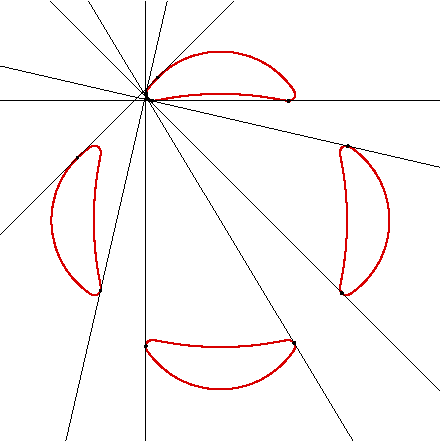
\includegraphics[height=2in]{main/Trott-cropped}}}
 \caption{The smooth plane quartic
$144 ( x^4 + y^4 ) - 225 ( x^2 + y^2 ) + 350 x^2 y^2 + 81 = 0$,
known as the Trott curve
\protect\citeyear{Trott}, has all 28 bitangents real.
\index{Trott quartic}%
(Only seven are shown for neatness. The involution $x \leftrightarrow -x$ gives
$7-1 =6$ more, then $y\leftrightarrow -y$ gives $13-2=11$ more, and
$x\leftrightarrow y$ the
remaining four.)}
\label{trott}
\end{figure}

The bitangents to a smooth plane quartic $C$ (a canonical curve of genus
3) have a special significance: since $4 = 2 \times 2$, if $D = p+q$ is
a bitangent, then the divisor $2D$ comprises the complete intersection
of $C$ with a line; in other words, we have a linear equivalence
$$
2D \sim K_C
$$
or equivalently the invertible sheaf $\cO_C(D)$ is a
square root of the canonical sheaf
\index{square root!of canonical sheaf}%
\index{canonical sheaf!square root of}%
of $C$. Because of their appearance in the theory of
\index{theta function}%
theta functions,
Riemann
\index{Riemann, Georg Friedrich Bernhard}%
named the square roots of the canonical sheaf
\emph{theta characteristics}.

How many such square roots are there? If $\cL$ and $\cM$ are invertible
sheaves with $\cL^2 = \cM^2 = K$, then $\cL$ and $\cM$ differ by an
invertible sheaf of order 2; that~is,
$$
\cM = \cL \otimes \cF, \quad \text{where} \quad \cF \otimes \cF \sim
\cO_C.
$$
In other words, $\cF$ is an invertible sheaf of degree 0 and, having
fixed $\sL$,  the other sheaf, $\cM$, corresponds to a point of order
2 in the
Picard group
\index{Picard group}%
$\Pic_0(C)$. Since we've seen that $\Pic_0(C) =
\Jac(C)$ is a complex torus of dimension
$g =\nobreak 3$\emdash the quotient of $\CC^3$
by a lattice $\Lambda \cong \ZZ^6$\emdash we see that there are $2^6 = 64$
such invertible sheaves, and thus, given that there is some invertible
sheaf $\cL$ satisfying $\cL^2 \cong K_C$, there are exactly $64 = 2^{2g}$
of them.

The reader will have noticed that the number 64 of theta characteristics
does not agree with the number 28 of bitangents. The reason is
that
bitangents correspond to \emph{effective} divisors $D$ with $2D
\sim K$, while a theta characteristic $\cL$ may have $h^0(\cL) = 0$,
that is, may not correspond to an effective divisor.
This situation also occurs in other genera.
What can we say about the dimensions $h^0(\cL)$ of the space of sections
of the theta characteristics on $C$?

 There is a beautiful partial answer to this question, which can be
 deduced from a remarkable fact: the dimension $h^0(\cL)$ of the space
 of sections of a theta characteristic mod 2 is invariant in families.
We will now
sketch the necessary results; see \cite{MumfordPaper} and \cite{JHPaper}
for a full treatment.

 \begin{theorem}
 \label{locally constant sign}
 Let $\cC \to B$ be a family of smooth curves, and $\cL_b$ a family of
 theta characteristics on the curves in this family\emdash in other words, an
 invertible sheaf $\cL$ on $\cC$ such that $(\cL|_{C_b})^2 \cong K_{C_b}$
 for each $b \in B$.
If
$f : B \to \ZZ/2$
is defined by
 $$
 f(b) = h^0(\cL|_{C_b}) \;  \; (\mathrm{mod\ } 2),
 $$
then $f$ is locally constant.
\unif
\end{theorem}

We say that a theta characteristic $\cL$ is \emph{even} or \emph{odd}
\index{theta characteristic!parity}%
according to the parity of $h^0(\cL)$. Given the irreducibility of the
space of smooth irreducible curves of genus $g$ (which we'll discuss
in Chapter~\ref{CurvesModuliChapter}),
Theorem~\ref{locally constant sign}
suggests that all curves of genus $g$ have the same number of
even (equivalently, of odd) theta characteristics, and this is in fact
the case.

\begin{theorem}
\label{number of theta characteristics}
If $C$ is a curve of genus $g$, then of the $2^{2g}$ theta characteristics
\index{theta characteristic!number of --s}%
on $C$ there are $2^{g-1}(2^g + 1)$ even theta characteristics and
$2^{g-1}(2^g-1)$ odd theta characteristics.
\unif
\end{theorem}

Using Theorem ~\ref{locally constant sign} and the connectedness of the
moduli space of curves,
Theorem~\ref{number of theta characteristics} is reduced to the case when
$C$ is hyperelliptic. We will
compute the number of theta characteristics in the hyperelliptic case
later in this section (page~\pageref{theta characteristic count}).

For
a nonhyperelliptic curve $C$ of genus 3, the
dimension $h^0(\cL)$ of a theta characteristic $\cL$ cannot be $\geq 2$, so
the odd theta characteristics are exactly the effective theta
characteristics, and  this says
that there are $2^{g-1}(2^g-1)
= 28$ effective theta characteristics corresponding to the 28 bitangents.
\index{bitangent!to a plane quartic}%


We will present  a proof of Theorem~\ref{locally constant sign} using
an ingenious construction of
Mumford's,
\index{Mumford, David}%
after explaining the necessary facts about
quadratic forms
\index{quadratic form}%
in an even
number of variables.
\smallbreak

\begin{fact}
\label{isotropic facts}
Suppose that $V$ is a $2n$-dimensional complex vector space with a
nondegenerate
bilinear form
\index{bilinear form}%
$Q$. An
\emph{isotropic subspace} for $Q$ is a subspace $\Lambda \subset V$ such that
\index{isotropic subspace}%
$Q(\Lambda, \Lambda) = 0$.

 \begin{enumerate}
\item The maximal isotropic subspaces for $Q$ have dimension $n$.

\item The set of maximal isotropic subspaces for $Q$ is a subvariety of
the
Grassmannian
\index{Grassmannian}%
$G(n,V)$, of dimension $\tbinom{n}{2}$, that has exactly
two connected components.

\item If $\Lambda, \Lambda' \subset V$ are any two maximal isotropic
subspaces, then
$$
\let\quad\enspace
\null\hskip\leftmargini
\dim(\Lambda \cap \Lambda') \equiv n \text{ (mod 2)} \quad \iff \quad
\Lambda, \Lambda' \text{ \,belong to the same ruling.}
$$
\end{enumerate}

A  proof is given in \cite[pp.~735--740]{Griffiths-Harris1978}.
\end{fact}

\begin{remark}
The first assertion in
Cheerful Fact \ref{isotropic facts}
is
elementary: since the map
$\widetilde Q : V \ruto \cong V^*$ associated to the form $Q$ carries
\index{isotropic subspace}%
an isotropic subspace to its annihilator, there can't be an isotropic
subspace of dimension $>n$; and similarly if $\Lambda \subset V$ is any
isotropic subspace of dimension $<n$ we can include $\Lambda$ in a larger
isotropic subspace by adding any vector $v$ with $\overkern20 Q(v,v) = 0$
for the induced bilinear form $\overkern20 Q$ on $\ann(\Lambda)/\Lambda$.

The second and third assertions are less elementary, but the reader may
already have seen the first two nontrivial cases of each:
\end{remark}

\begin{example}
When $n=2$ the form $Q$ corresponds to a smooth quadric surface
in $\PP^3` `$, and the lines on this surface correspond to the isotropic
2-planes in $\CC^4` `$. There are two rulings by lines, and lines of
opposite rulings meet in a point, while lines of the same ruling are
either disjoint or equal.
\end{example}

\begin{example}
When $n=3$, the Grassmannian $\GG(1,3)$, in its
Pl\"ucker embedding,
\index{Pl\"ucker embedding}%
\index{Grassmannian}%
is a smooth quadric in $\PP^5` `$. The isotropic subspaces in the two distinct
components are easy to describe: in one component they are the projective
2-plane of lines containing a given point $p \in \PP^3` `$. In the other
component they are  the planes corresponding to the lines contained in a
given plane $H \subset \PP^3` `$. These families visibly satisfy property (3) above.
See Exercise~\ref{G13}.
\end{example}

\begin{proof}[Proof of Theorem~\ref{locally constant sign}] Suppose that $C$ is a smooth curve of genus $g$, and
let $\cL$ be
an invertible sheaf on $C$ with $\cL^2 \cong K_C$\emdash that is, a theta
characteristic. Choose a divisor $D = p_1 + \dots + p_n$ of degree $n>
g-1$ consisting of distinct points, and let $V$ be the $2n$-dimensional
vector space
$$
V \colonequals  H^0( \cL(D) / \cL(-D) ).
$$
From the exact sequence
$$
0\to \cL(-D) \to \cL(D) \to \cL(D)/\cL(-D) \to 0
$$
we see that
the sheaf $ \cL(D) / \cL(-D)$ is supported on $D$, with stalk
isomorphic to $\cO_p/\gm_{C,p}^2$ of dimension 2 at each $p \in D$. We
can define a bilinear form on $V$ by setting
\index{residue}%
$$
Q(\sigma, \tau) \colonequals  \sum_i \Res_{p_i}(\sigma \tau)
\vspace*{-3pt}
$$
where we use the isomorphism $\cL^2 \cong K_C$ to identify the product
$\sigma\tau$ with a rational differential.

We now introduce two isotropic subspaces for $Q$.
The first is
$$
\Lambda \colonequals  H^0( \cL / \cL(-D) ),
$$
which
is isotropic because the product
of two of its elements
corresponds to a regular differential, and so has no residues.
Second, we set
$$
\Lambda' \colonequals  \im\left( H^0(\cL(D)) \to H^0( \cL(D) / \cL(-D) ) \right)
.
$$
Since  $H^0(\cL(-D)) = 0$, the map is injective and according to
the Riemann--Roch theorem we have
$h^0(\cL(D)) = n$, so this is again an $n$-dimensional
subspace of~$V$; it's isotropic because the sum of the residues of a
global rational differential on $C$ is 0. Finally,
$$
H^0(\cL) \cong \Lambda \cap \Lambda',
$$
and Theorem~\ref{locally constant sign} follows.
\end{proof}




\subsection*{Counting theta characteristics (proof of Theorem~\ref{number of theta characteristics})}

One
way to count the number of odd and even theta characteristics on
\label{theta characteristic count} % used for page number
a curve of genus $g$ is  to describe
them
explicitly in the case of
a hyperelliptic curve and
use Theorem~\ref{locally constant sign}
to deduce the corresponding statements for any smooth curve of genus~$g$.
The reader
may wish to
try a relatively simple case in
Exercise~\ref{theta char on genus 2} before looking at the general
case below.
We start with some preliminary calculations:

\begin{lemma}
\label{summing binomials}
For any positive integer $n$,
we have
\let\binom\mbinom
\begin{gather}
\let\;\relax
\sum_{k=0}^n \binom{2n}{2k} \; = \; \sum_{k=0}^{n-1} \binom{2n}{2k+1}
\; = \; 2^{2n-1}
,\\
\sum_{k=0}^n \binom{4n}{4k} = 2^{4n-2}  + (-1)^n 2^{2n-1},
\quad \sum_{k=0}^{n-1} \binom{4n}{4k+2} = 2^{4n-2} - (-1)^n  2^{2n-1}
,\\
\sum_{k=0}^n \binom{4n+2}{4k+1} = 2^{4n} + (-1)^n 2^{2n},
\quad \sum_{k=0}^{n-1} \binom{4n}{4k+3} = 2^{4n} - (-1)^n  2^{2n}
.
\end{gather}
\end{lemma}

\begin{proof}
\let\binom\mbinom
Equality (1) is
elementary; by the binomial theorem, we have
$$
2^{2n} = (1+1)^{2n} = \sum_{l = 0}^{2n}@\binom{2n}{l} \quad \text{and}
\quad 0 = (1-1)^{2n} = \sum_{l = 0}^{2n}@(-1)^l\binom{2n}{l}
,
$$
and taking the sum and the difference of these two equations yields the
result.

The equalities in (2) follow
similarly by applying the binomial theorem to the
expression $(1 + i)^{4n} = (-1)^n2^{2n}$. Equating the real parts, we have
$$
\sum_{k=0}^n \binom{4n}{4k} - \sum_{k=0}^{n-1} \binom{4n}{4k+2} =
(-1)^n2^{2n}
,
$$
while by
(1)
we have
$$
\sum_{k=0}^n \binom{4n}{4k} + \sum_{k=0}^{n-1} \binom{4n}{4k+2} =
2^{4n-1}.
$$
Taking the sum and difference of these equations yields the desired
formulas.

For (3)
we apply the binomial theorem to the expression $(1 + i)^{4n+2} =
 (-1)^n2^{2n+1}i$. Equating the imaginary parts, this gives
\let\;\relax
$$
\sum_{k=0}^n \binom{4n+2}{4k+1} - \sum_{k=0}^{n-1} \binom{4n+2}{4k+3}
\; = \; (-1)^n2^{2n+1}
,
$$
whereas by
(1),
$$
\sum_{k=0}^n \binom{4n+2}{4k+1} + \sum_{k=0}^{n-1} \binom{4n+2}{4k+3}
\; = \; (-1)^n 2^{4n+1}
,
$$
and as before taking the sum and difference
yields the
result.
\end{proof}

We will count the number of theta characteristics on a hyperelliptic
curve in terms of sums of subsets of the ramification points, so we need
to know what linear equivalences exist among sums of these subsets:

\begin{lemma}
\label{ramification point relations}
Let $C$ be the hyperelliptic curve of genus $g$ expressed as a 2-sheeted
cover of $\PP^1$ with ramification points $p_1,\dots,p_{2g+2}$. The
divisor class of
 any half of the ramification points is equal to the divisor class of
 the other half, but there are no
 smaller relations. More precisely,
 let $I_1,I_2$ be subsets of $\{1,\dots 2g+2\}$
and set
$$
D_i = \sum_{j\in I_i} p_j.
$$
The divisors $D_1,D_2$ are linearly equivalent if and only if $I_1 `= I_2$
or they
have the same cardinality $g+1$ and $I_1`\cup I_2 = \{1,\dots, 2g+2\}$.
\end{lemma}

\begin{proof}
The ``if'' part is simply
Corollary~\ref{relation on ramification points} above.

For the ``only if'' part, subtracting whatever points $D_1$ and $D_2$
have in common we may suppose
that $I_1`\cap I_2 = \emptyset$. If $D_1\sim D_2$, it follows at once that
they have the same degree, $d\leq g+1$, and we must show that either $d=0$
or $d=g+1$.

We have $D_1\sim D_2$
if and only if
$D_1+D_2\equiv 2D_1$. If
$d\leq g$ we have $r(2D_1) = d$: for $d<g$ this is
the extremal case of
Clifford's theorem,
\index{Clifford's theorem}%
while for $d = g$ this follows
simply from the
Riemann--Roch formula.
\index{Riemann--Roch formula}%
Thus in case $d \leq g$ every divisor in $|2D_1|$
is a sum of $d$ fibers of the
2 to 1 map of $C$ to $\PP^1` `$, and for such a divisor to be a sum of
distinct points $p_i$
the degree $d$ must be 0, concluding the argument.
\end{proof}

Returning
now
to the counting, let $C$ be the hyperelliptic curve of genus
$g$, \null
expressed as a 2-sheeted cover of $\PP^1` `$, with ramification points
$p_1,\dots,p_{2g+2}$.

First of all, if we denote the class of the unique $g^1_2$ on $C$ by
$E$, and $D$ is any theta characteristic, then $D+E$ will be effective,
and so we can write
$$
D \sim mE + F
$$
with $-1 \leq m \leq (g@{-}@1)/2$ and $F$ the sum of $g-1-2m$ distinct
points $p_i$.
This representation is unique unless
$m=-1$; in that case, we note that the sum of $g+1$ of the branch
points of $C$ is linearly equivalent to the sum of the other $g+1$ by
Corollary~\ref{relation on ramification points}. Thus the total number of
theta characteristics is a sum of binomial coefficients; if $g$ is odd,
it is
$$
\let\binom\mbinom
\binom{2g+2}{0} + \binom{2g+2}{2} + \binom{2g+2}{4} + \dots +
\binom{2g+2}{g-1} + \frac{1}{2}\binom{2g+2}{g+1}
$$
and similarly if $g$ is even it is
$$
\let\binom\mbinom
\binom{2g+2}{1} + \binom{2g+2}{3} + \binom{2g+2}{5} + \dots +
\binom{2g+2}{g-1} + \frac{1}{2}\binom{2g+2}{g+1}.
$$
In either case, we are adding up every other entry in the $(2g+2)$-nd
row of Pascal's triangle, starting from the left and ending up with one
half of the middle term. This sum is exactly one half of the sum of every
other entry in the whole row; by the first part of
Lemma~\ref{summing binomials}
this
equals
$\sfrac{1}{4} \cdot 2^{2g+2} = 2^{2g}$.

Finally, we can add up the number of even and odd theta characteristics
separately simply by taking every other term in the sums above;
using
equalities (2) and (3) in
Lemma~\ref{summing binomials}
(in case $g$ is odd and even, respectively) we can conclude that $C$
has $2^{g-1}(2^g-1)$ odd theta characteristics and $2^{g-1}(2^g+1)$
even theta characteristics. By Theorem~\ref{locally constant sign} and
the connectedness of the space of smooth irreducible curves of genus
$g$, this count then holds for all curves of genus $g$, establishing
Theorem~\ref{number of theta characteristics}.
\qed

 It is also
 possible to describe the configurations of odd and even theta
characteristics as subsets of the set $S$ of all theta characteristics,
which as we've seen is a principal
homogeneous space for the group
$\Jac(C)_2 \cong (\ZZ/2\ZZ)^{2g}$ of
points of order 2 on the Jacobian.
\index{Jacobian!points of order 2}%
 This leads to an alternative proof of
Theorem~\ref{number of theta characteristics} as in \cite{JHPaper}.

\begin{fact}
There is more to say about the configuration of theta characteristics.
As noted, if we choose any theta characteristic on a curve $C$, we may
 identify the set $S^-$ of odd theta characteristics with a subset of the
 group $\Jac(C)_2$ of points of order 2 on the Jacobian of $C$. We might
 expect that some 4-tuples of these points will add up to 0 in $\Jac(C)$;
 in other words, there should exist some 4-tuples $\cL_1,\dots,\cL_4
 \in S^-$ such that
$$
\cL_1\otimes \dots \otimes\cL_4 = 2K_C.
$$
What this means in the case of genus $g=3$ is that among the 28 bitangents
\index{bitangent!to a plane quartic}%
to a smooth plane quartic curve $C$, there are some subsets of 4 whose
eight points of tangency form the intersection of $C$ with a plane
conic. From the more detailed knowledge of the configuration $S^-$
we can say how many. Indeed, the number was first found by Salmon
\index{Salmon, George}%
\citeyear{MR0115124};
it is 315.
\end{fact}

\section{Exercises}
 \begin{exercise}
  We have seen that a curve $C$ of genus $g=1$ is expressible as a
  2-sheeted cover of $\PP^1$ branched over four points; that is, as
  the smooth projective curve associated to the affine curve $C^\circ
  \subset \AA^2$ given by $y^2 -
\smash{\prod_{i=1}^{\smash{\lower1.5pt\hbox{$\ssty4$}}} (x-\lambda_i)}$.
  Show that
  the closure $\overkern22{C^\circ}$ of $C^\circ \subset \AA^2$ in either
  $\PP^2$ or $\PP^1 \times \PP^1$ consists of the union of $C^\circ$ with
  one additional point, with that point a tacnode of $\overkern22{C^\circ}$
  in either case.
  \tohint{6-01}
  \end{exercise}

\begin{exercise}
Find the number of
3-sheeted covers
\index{3-sheeted cover}%
$C \to \PP^1$ of genus $g$ with
simple branching except for one point of
\index{simple branch point}%
\index{branch point!simple}%
total ramification
\index{total ramification}%
(that is,
one point with just a single preimage point.)
\tohint{6-01}
\end{exercise}

\begin{exercise}
Let $C$ be a curve of genus $g$. How many
unramified double covers
of $C$
\index{2-sheeted cover!unramified}%
are there?
\tohint{6-03}
\end{exercise}

\begin{exercise}
Show that unramified
double covers
\index{2-sheeted cover}%
of a smooth curve $C$ are in one-to-one
correspondence
with invertible sheaves $\sL$ on $C$ such that $\sL^2 \cong \sO_C$,
that is with the
2-torsion points
\index{Jacobian!points of order 2}%
of $\Jac(C)$.
\tohint{6-04}
\end{exercise}

\begin{exercise} Let $E$ be a curve of genus 1, and $q_1,\dots,q_b \in
E$. How many double covers $C \to E$ are there branched over the $q_i$?
\tohint{6-05}
\end{exercise}

\begin{exercise}
\label{ideal of genus 2 degree 5}
In
this
exercise, we ask you to complete the
earlier
description
of the ideal of a quintic space curve of
genus 2,
keeping the notation of page~\pageref{genus 2 quintic}.

Show that for any pair of lines $L, L'$ of the appropriate ruling of $Q$,
\index{quintic!of genus 2}%
the three polynomials $Q$, $S_L$ and $S_{L'}$ generate the homogeneous
ideal $I(C)$. Find relations among them. Write out the minimal resolution
of $I(C)$.
\tohint{6-06}
\end{exercise}

\begin{exercise}
% an easy case the reader can do before reading the general treatment.
\label{theta char on genus 2}
 Let $C$ be a curve of genus 2, expressed as a 2-sheeted cover of $\PP^1$
 with ramification points $p_1,\dots,p_6$. In this exercise we will
 count the number of
 even and odd theta characteristics.
The text contains the count for a hyperelliptic curve of any genus;
we offer
the case of genus 2 as a warmup.
 \begin{enumerate}
 \item Show that the theta characteristics on $C$ are either of the
 form $\cL = \cO_C(p_i)$ or of the form $\cL = \cO_C(p_i + p_j - p_k)$
 with $i, j, k$ distinct.
 \item Show that in the first case we have $h^0(\cL) = 1$, and in the
 second case we have $h^0(\cL) = 0$.
 \item Finally, show that there are six of the former kind, and 10 of
 the latter, making $2^4 = 16$ in all.
 \tohint{6-07}
 \end{enumerate}
 \end{exercise}

\begin{exercise}
\label{nodal quartic}
Let $C$ be a  curve of genus 2 and let $\sL\in \Pic_4(C)$ be an invertible
sheaf of the form $\sL = K_C(p+q)$ with $p \neq q$ and $p+q \not\sim K_C$
as in~\ref{p+q not g12}. Show that
\begin{enumerate}
\item $h^0(\sL(-2r))= 1$ for any point $r \in C$, and
\item $h^0(\sL(-2p-2q)) = 0$.
\end{enumerate}
Deduce from this that the map $\phi_\sL$ is an immersion, and that the
tangent lines to the two branches of $\phi_\sL(C)$ at the point $\phi_\sL(p)
= \phi_\sL(q)$ are distinct, meaning the point $\phi_\sL(p) = \phi_\sL(q)$
is a node of $\phi_\sL(C)$.
\tohint{6-08}
\end{exercise}

\begin{exercise}
\label{G13}
We can represent any line in $\PP^3$ as the row space of a $2\times 4$ matrix by choosing
 2 points on the line and
using their
coordinates as the rows. The \emph{Pl\"ucker coordinates} of the line are
\index{Pl\"ucker coordinates}%
the six $2\times 2$ minors
$$
\{p_{i,j}\}_{0\leq i<j\leq 3}
$$
of this matrix. They are independent, up to a common scalar multiple,
of the two points chosen, and define the \emph{Pl\"ucker embedding}
\index{Pl\"ucker embedding}%
of the
Grassmannian
\index{Grassmannian}%
$\GG(1,3)$ in $\PP^5` `$.

The minors $p_{i,j}$  satisfy a nonsingular quadratic equation: if we
stack two copies of the $2\times 2$
matrix to produce a $4\times 4$ matrix, its determinant is zero, and
the Laplace expansion of this determinant
is the \emph{Pl\"ucker equation}
\index{Pl\"ucker equation}%
$$
p_{0,1}p_{2,3}-p_{0,2}p_{1,3}+p_{0,3}p_{1,2} = 0.
$$

\begin{enumerate}
\item Show that the quadratic form
$
Q = p_{0,1}p_{2,3}-p_{0,2}p_{1,3}+p_{0,3}p_{1,2}
$
is non\-singular, and deduce that it generates the ideal of $\GG(1,3)$
in $\PP^5` `$.
\item
Write the bilinear form corresponding to $Q$ as the determinant of a
matrix, and deduce that
two points in $\GG(1,3)$ correspond to vectors that pair to 0 if and
only if they correspond to lines that intersect.
\item Deduce that a maximal isotropic subspace for $Q$ corresponds either to
the set of lines containing a given point or the set of lines contained
in a given plane; and that two such sets of lines
of the same type
meet in a single point or coincide.
\end{enumerate}
\end{exercise}


%header and footer for separate chapter files

\ifx\whole\undefined
\documentclass[12pt, leqno]{book}
\usepackage{graphicx}
\usepackage{eps-to-pdf}
\input style-for-curves.sty
%\input sl-macros.sty
\usepackage{hyperref}
\usepackage{showkeys} %This shows the labels.
\usepackage{msribib}
\usepackage{pdfpages}
\usepackage{draftwatermark}
\SetWatermarkText{DRAFT:\ \today}
\SetWatermarkScale{2}
\SetWatermarkColor[gray]{0.9}

%\usepackage{SLAG,msribib,local}
%\usepackage{amsmath,amscd,amsthm,amssymb,amsxtra,latexsym,epsfig,epic,graphics}
%\usepackage[matrix,arrow,curve]{xy}
%\usepackage{graphicx}
%\usepackage{diagrams}
%
%%\usepackage{amsrefs}
%%%%%%%%%%%%%%%%%%%%%%%%%%%%%%%%%%%%%%%%%%
%%\textwidth16cm
%%\textheight20cm
%%\topmargin-2cm
%\oddsidemargin.8cm
%\evensidemargin1cm
%
%%%%%%Definitions
%\input preamble.tex
%\input style-for-curves.sty
%\def\TU{{\bf U}}
%\def\AA{{\mathbb A}}
%\def\BB{{\mathbb B}}
%\def\CC{{\mathbb C}}
%\def\QQ{{\mathbb Q}}
%\def\RR{{\mathbb R}}
%\def\facet{{\bf facet}}
%\def\image{{\rm image}}
%\def\cE{{\cal E}}
%\def\cF{{\cal F}}
%\def\cG{{\cal G}}
%\def\cH{{\cal H}}
%\def\cHom{{{\cal H}om}}
%\def\h{{\rm h}}
% \def\bs{{Boij-S\"oderberg{} }}
%
%\makeatletter
%\def\Ddots{\mathinner{\mkern1mu\raise\p@
%\vbox{\kern7\p@\hbox{.}}\mkern2mu
%\raise4\p@\hbox{.}\mkern2mu\raise7\p@\hbox{.}\mkern1mu}}
%\makeatother

%%
%\pagestyle{myheadings}

%\input style-for-curves.tex
%\documentclass{cambridge7A}
%\usepackage{hatcher_revised} 
%\usepackage{3264}
   
\errorcontextlines=1000
%\usepackage{makeidx}
\let\see\relax
\usepackage{makeidx}
\makeindex
% \index{word} in the doc; \index{variety!algebraic} gives variety, algebraic
% PUT a % after each \index{***}

\overfullrule=5pt
\catcode`\@\active
\def@{\mskip1.5mu} %produce a small space in math with an @

\title{A Chapter from ``The Practice of Algebraic Curves"}
\author{\copyright David Eisenbud and Joe Harris}
%%\includeonly{%
%0-intro,01-ChowRingDogma,02-FirstExamples,03-Grassmannians,04-GeneralGrassmannians
%,05-VectorBundlesAndChernClasses,06-LinesOnHypersurfaces,07-SingularElementsOfLinearSeries,
%08-ParameterSpaces,
%bib
%}

\date{\today}
%%\date{}
%\title{Curves}
%%{\normalsize ***Preliminary Version***}} 
%\author{David Eisenbud and Joe Harris }
%
%\begin{document}

\begin{document}
\maketitle

\pagenumbering{roman}
\setcounter{page}{5}
%\begin{5}
%\end{5}
\pagenumbering{arabic}
\tableofcontents
\fi


\chapter{Fine moduli spaces}
\label{Moduli chapter}
\label{ModuliChapter}

\section{What is a moduli problem?}

Algebraic geometry is special among geometric theories in
that
the objects involved\emdash varieties,  schemes or maps between
them\emdash can be parametrized by other varieties or schemes. The set
of submanifolds of a given manifold, or more generally of maps between
two given manifolds, seems too large to be given the structure of a
finite-dimensional manifold itself. By contrast, any algebraic variety
is specified by a finite collection of polynomials, which in turn have
a finite number of coefficients, so it's not too far-fetched that the
set of all varieties with specified numerical invariants, or
morphisms between two given varieties, could be given the structure of
a ``moduli space'' that is a variety (or scheme or\dots) in its own
right.

For an example\emdash perhaps the original one\emdash projective plane
curves of degree $d$
are in natural one-to-one correspondence with the forms of degree $d$
modulo the group of nonzero scalars\emdash that is, with the points of
the dual of the projective space
$ \PP(H^0(\sO_{\PP^2}(d)))=\PP^{\sbinom{d+2}{2}-1} $.
Thus, for example, plane cubics are parametrized by $\PP^{9}$, and a
family $\cC \to B$ of cubics corresponds to a map $\phi: B \to \PP^9` `$ (Figure~\ref{cubic family}).
In this chapter, we'll give a general framework for the notion of moduli
space, introducing the main examples that we will treat in this book.

\begin{figure}
\vskip-14pt
$
  \vcenter{\hbox{\includegraphics[width=0.84in,trim=0 27 7 25,clip]{"main/Fig06-1a"}}}\hskip0.6em
  \vcenter{\hbox{\includegraphics[width=0.7in]{"main/Fig06-1b"}}}\quad
  \vcenter{\hbox{\includegraphics[width=0.7in]{"main/Fig06-1c"}}}\quad
  \vcenter{\hbox{\includegraphics[width=0.7in]{"main/Fig06-1d"}}}
$
\vskip-3pt
 \caption{A one-parameter family of plane cubics.}
 \label{cubic family}
\end{figure}

There are several ways in which the possibility of making moduli spaces
has been useful in algebraic geometry. First, the existence of a moduli
space that  parametrizes objects of a certain type allows us to speak
of the ``general \null object,'' meaning that we allow ourselves to avoid the
 properties of ``special objects'' parametrized by closed subvarieties
of the moduli space. For example, we can make precise sense of the
statement, ``The general plane curve of degree $d$ is smooth." It means 
that the set of smooth curves corresponds to an open subset of the projective space $\PP^{\sbinom{d+2}{2}-1} $.
 We have already used this
possibility in many places in this book.

Second, it allows us to speak coherently about
families of objects. Some moduli spaces carry \emph{universal families},
\index{universal family}%
and every nice family of the sort of objects
they parametrize is pulled back from this one by a unique map.

This idea was already exploited informally in the nineteenth century in
\index{historical context}%
\index{preservation of number}%
the guise of ``preservation of number,'' used to count configurations of
points or curves with a given property by specializing the
data, and we have also exploited this idea in
Chapter~\ref{JacobianChapter} to explain the count of odd and even
theta characteristics on a general curve by appealing to the existence
of a specialization to a hyperelliptic curve. In a related manner, we
have already seen how the fact that invertible sheaves of degree $d$
on a curve $C$ are parametrized by a $g$-dimensional variety allows us
to prove the $g+3$ theorem (Theorem~\ref{g+3 theorem}).

Third, to the extent that we can describe the intersection theory of a
moduli space, it opens up the possibility of doing
\blue{enumerative geometry}
\index{enumerative geometry}%
on it to count solutions of geometric problems\emdash and in particular
to prove the existence of solutions. For example, knowing that the
\index{P@$\PP^3$!any 4 curves intersect a common line}%
parameter space for lines in $\PP^3$ is the Grassmannian $\GG(1,3)$,
\index{Grassmannian $\GG(1,3)$}%
a projective variety of dimension 4, and that the condition that the
set of lines meeting a given curve of degree $d$
is a divisor linearly equivalent to  $d$ times the hyperplane section
(Figure~\ref{Chow degree}), we can conclude  that there exists a line
in $\PP^3$ meeting any four given curves \cite[Section 3.4.1]{3264}. We
will use the same idea to prove the much deeper existence of certain
linear series on all curves (the existence half of the Brill--Noether
theorem, discussed in Chapter~\ref{Brill--Noether}).

\begin{figure}
\centerline {\includegraphics[height=1.4in]{"main/Fig06-2"}}
 \caption{A general  one-parameter linear family of lines in $\PP^3$\emdash that is, the family of lines
 contained in a general plane and passing through a general point in that plane\emdash meets a space curve $C$ in
 $\deg C$ points.}
 \label{Chow degree}
\end{figure}

In modern terms, a \emph{moduli problem}
\index{moduli problem}%
consists of a class of objects
in algebraic geometry\emdash schemes, subschemes of a given scheme,
maps of schemes,
sheaves on schemes, typically defined by some common
attributes\emdash and a notion of what it means to have a \emph{family}
\index{family}%
of these objects parametrized by a scheme $B$. The notion is formalized
in the idea of a \emph{moduli functor},
\index{moduli functor}%
which associates to each scheme $B$ the set of families over $B$ of the
given sort. Examples will make this vague notion more concrete.

%\subsection*{Some moduli problems}

%\begin{enumerate}
%\label{list of moduli problems}

\begin{example}[effective divisors on a given curve] The objects are
\index{moduli functor}%
\index{effective divisor!family of --s on a curve}%
effective divisors of given degree on a given smooth, projective curve
$C$. A family of such divisors is a subscheme $\cD \subset B \times C$,
flat of degree $d$ over $B$.
Here we are using
the equivalence between divisors of degree $d$ on a smooth curve and
degree $d$ subschemes of the curve. The moduli space is the $d$-th
\blue{symmetric power}
\index{symmetric power}%
$C_d$ of $C$, discussed in Section~\ref{symmetric section}.
\end{example}

\begin{example}[invertible sheaves on a given curve] The objects are
\index{invertible sheaves!family of --s on a curve}%
invertible sheaves on a given smooth projective curve $C$. A family
over a scheme $B$ is an equivalence class of invertible sheaves $\cL$
on $B \times C$ whose restriction to each fiber of $B \times C$ over
$B$ has degree $d$, where two families $\cL$ and $\cL'$ on $B \times
C$ are equivalent if $\cL\cong \cL' \otimes \cM$, where $\cM$ is  an
invertible sheaf pulled back from $B$. Usually one restricts attention
to invertible sheaves
whose restrictions to each fiber $b\times C$ have a given degree $d$.
\index{Jacobian}%
\index{Picard variety}%
The moduli spaces are the \blue{Jacobian} and \blue{Picard varieties},
discussed in
Section~\ref{Picard section}.
\end{example}

\begin{example}[moduli of smooth curves] The objects are isomorphism
\index{smooth curve!moduli of --s}%
classes of smooth, projective curves of genus $g$. A family over $B$
is an equivalence class of smooth, projective morphisms $f : \cC \to B$
whose fibers are curves of genus $g$, where two such families $f, f'$
are equivalent if there is an isomorphism from the source of $f$ to
the source
of $f'$ making the
following diagram commute:
$$
\begin{diagram}[small]
\cC && \rTo^\cong && \cC'\\
&\rdTo_f&&\ldTo_{f'}\\
&&B
\end{diagram}
\vspace*{3pt}
$$
The moduli spaces $M_g$ of curves are harder to construct, and we will
have a separate discussion of them in
Chapter~\ref{CurvesModuliChapter}. Nonetheless,
it will be useful at several points in this chapter to assume their
existence.
\end{example}

\begin{example}[Hurwitz spaces] An object is a smooth projective curve $C$
\index{Hurwitz space}%
of a given genus, together with a map $f: C\to \PP^1$ of given degree, up
to isomorphisms of the curves that commute with the map, as in this diagram:
$$
\begin{diagram}[small]
C && \rTo^{\cong} && C'\\
&\rdTo_f&&\ldTo_{f'}\\
&&\PP^{1}
\end{diagram}
$$
A family over $B$ is a family $\cC \to B$ of smooth projective curves
of a given genus, together with flat map $\cC \to B\times \PP^{1}$
of degree $d$.
 Often the allowable ramification indices are specified. We will discuss
 the simplest Hurwitz scheme in Chapter~\ref{CurvesModuliChapter}.
\end{example}

\begin{example}[Severi varieties] The objects are plane curves
\index{Severi variety}%
\label{Severi}%
of given degree $d$ and geometric genus $g$. If $g \neq \tbinom{d-1}{ 2}$
the curves will necessarily be singular, but are often
constrained to have only mild singularities, usually only nodes. We will
discuss
Severi varieties
in Chapter~\ref{CurvesModuliChapter}.
\end{example}

\begin{example}[Hilbert schemes] The objects are subschemes of a given
\index{Hilbert scheme}%
projective space;   a family over $B$ is a subscheme $\cC \subset B \times
\PP^r` `$, flat over $B$. Since the Hilbert polynomials of the fibers
of a
\blue{flat family}
\index{flat family}%
are all equal
\cite[Chapter III, \S9]{Hartshorne1977},
the Hilbert scheme is the disjoint union of subschemes corresponding to
particular Hilbert polynomials, and these subschemes are of finite type.
\index{finite type}%
If $B$ is reduced then the flatness condition is equivalent to the
constancy of the Hilbert polynomial (\cite[Theorem 9.9]{Hartshorne1977} or \cite[Chapter III, \S 3.2]{DE-JH-schemes}).

In Chapter~\ref{HilbertSchemesChapter} we
study the
open set consisting of smooth curves $C\subset \PP^{r}$ of given degree
and genus.
\end{example}

\section{What is a solution to a moduli problem?}

Typically what we want from a solution to a
\blue{moduli problem}
\index{moduli problem}%
is to
understand all possible families of the objects
in question. In particular, the individual objects should be in natural
\index{natural correspondence}%
one-to-one correspondence with the closed points of the
moduli space.  The word \emph{natural} is the key. Most of the time,
the set of objects we are interested in has
the cardinality of the continuum,
as do all positive-dimensional varieties $M$ over $\CC$, so a mere
bijection between the points of $M$ and the objects to be parametrized
is meaningless.

In the nicest situations there is a
\blue{\emph{universal} family}
\index{universal family}%
$\phi:
\cX\to M$ of these objects over $M$,
such that any family over a scheme $B$  is pulled back from the one on
$M$ via a unique morphism $B\to M.$  Such a space $M$ with its universal
family $\phi$, if it exists, is called a \emph{fine moduli space}. This
\index{fine moduli space}%
\index{moduli space!fine}%
can be expressed more abstractly but more succinctly by saying that the
moduli scheme \emph{represents the moduli functor}, which means there
is an isomorphism of functors
$$
\{ B \mapsto \text{families of } X \text{ over } B \} \cong \{ B\mapsto
\mathrm{{Mor}}_{\mathrm{ Schemes}}(B, M) \}.
$$
If $M$ is a fine moduli space then the identity map $M\to M$ corresponds
to the ``universal family'' $\phi: \cX \to M$.
The Hilbert scheme, as well as $\Div_d(C)$ and $\Pic_d(C)$ are fine moduli
spaces but the moduli space of curves
and the Hurwitz schemes are not.

If a fine moduli space and its universal family exist, then it is unique
up to unique isomorphism: given two avatars $M$ and $M'$
the universal family on $M$ corresponds to a map $M\to M'$, and we
similarly produce a map $M'\to M$. The pullback of the universal family
on $M$ by the composition of these two maps is again the universal family,
so the composition is the identity map.

Although the moduli space of curves and the Hurwitz spaces are not fine
moduli spaces, they are still defined
in a way that makes them unique, as we shall see below.

\def\eps{{\epsilon}}
One of the useful features of a fine moduli space is that it makes the
computation of tangent spaces relatively easy.
\index{tangent space}%
\index{Zariski tangent space}%
Recall that if $(R,\gm)$ is the local ring at a point $m$ on a variety
$\cM$ then the (Zariski) tangent
space to $M$ at $m$ is the vector space of linear functionals
$\Hom_{R/\gm}(\gm/\gm^2, R/\gm)$.   Assuming that
$R$ contains its residue field $k \colonequals  R/\gm$, such functionals
are precisely the restrictions to $\gm/\gm^2$ of the ring homomorphisms
$R \to k[\eps]/(\eps^2)$ inducing the identity on $k$.
 If $\cM$ is a fine moduli space for some functor $F$, then such maps
 are in one-to-one correspondence
with the set $F(E)$ of families over $E \colonequals
\Spec(k[\eps]/(\eps^2))$.

The vector space structure on the tangent space is also accessible from
this description:  the
 sum of tangent vectors corresponding to families $X_i \to E$ is the
 restriction to the diagonal
 $E \subset E\times E$
 of the product family $X_1 \times X_2 \to E\times E$.
Often one can to compute the tangent space to a moduli space before even
knowing that the moduli space exists!

\section{Hilbert schemes}
\label{hilbert scheme section}

The Hilbert scheme is a fine moduli space representing the functor of
\index{flat family!of subschemes}%
\index{subscheme!family of --s}%
\index{Hilbert scheme|(}%
flat families of subschemes of $\PP^r` `$,
that is, the functor that takes a scheme $B$ over $\CC$ to the set of
subschemes $\sX \subset B\times \PP^r$
that are flat over $B$; a morphism $f: B'\to B$ induces a map carrying
a family to the pullback of the family by $f$.

\begin{example}[the Hilbert scheme of plane curves]
\label{Hilb for plane curves}
Let $p(m) \colonequals  dm+1-\tbinom{d-1}{ 2}$ be the Hilbert polynomial of
a
\blue{plane curve}
\index{plane curve}%
of degree $d$, and consider the family
$\Hilb_{p(m)}(\PP^2)$
\index{notation!$\Hilb_{p(m)}$}%
of schemes $X \subset \PP^{2}$ having Hilbert polynomial $p$. Since
$\dim X = \deg p = 1$, $X$ has at least one component that is
1-dimensional. The union of such components must have degree
equal to $d$, the leading coefficient of $p(m)$. Since the Hilbert
polynomial  of this union is also equal
to $p(m)$ we see that $X$ is in fact a (possibly nonreduced and/or
reducible) plane curve of degree $d$. The space $\Hilb_{p(m)}(\PP^2)$
is the projective space $\PP^{\sbinom{d+2}{2}-1}$ of forms of degree $d$,
and the universal family is the projection
\blue{universal family}
\index{universal family}%
$$
\bigl\{@(x,F) \in \PP^2 \times \PP^{\sbinom{d+2}{2}-1} \mid F(x)=0@\bigr\} \to
\PP^{\sbinom{d+2}{2}-1}.
$$

More typically, the set of curves $C \subset \PP^r$ of degree $d$ and
genus $g$ corresponds to a subset of the Hilbert scheme parametrizing
subschemes of $\PP^r$ with Hilbert polynomial $p(m) = dm - g + 1$, though
not all schemes with this Hilbert polynomial are purely one-dimensional
subschemes, as we shall see.
\end{example}

In this section
we
compute
the Zariski tangent space to the Hilbert scheme at a point and
\index{Zariski tangent space}%
\index{Hilbert scheme!at a point}%
sketch the construction of the scheme itself. For a rigorous
treatment including many generalizations,  see \cite{HomogHilbert}
or \cite{MR2222646}. In Chapter~\ref{HilbertSchemesChapter}, we'll
describe  the
open subsets of smooth curves in the Hilbert schemes of curves of low
degree and genus in $\PP^3$ in more detail.

\subsection{The tangent space to the Hilbert scheme}
%\label{tan hilbert section}

Following the general recipe for tangent spaces to fine moduli spaces,
we need to understand
\blue{flat families}
\index{flat family}%
of projective schemes over $E \colonequals  \Spec
\CC[\eps]/(\eps^2)$. Recall
from
\cite[p.\,182]{Hartshorne1977},
for example,
that if
$X\subset \PP^r$ is a smooth subscheme then
 the normal bundle $\sN_{X/\PP^r}$ of $X$ in $\PP^r$ is defined in terms
 of the tangent bundles
 of $X$ and $\PP^r$ by the exact sequence:
$$
0\to \sT_X \ruto {\phi} \sT_{\PP^r}|_X \to \sN_{X/\PP^r} \to 0.
$$
Thus a global section of
$\sN_{X/\PP^r}$
\index{infinitesimal motion of a curve}%
can be thought of as an infinitesimal motion of~$X$ (Figure~\ref{perturbed
curve}).

\begin{figure}
\centerline {\includegraphics[width=1.35in]{"main/Fig06-0"}}
\vskip-5pt
 \caption{Infinitesimal perturbation of a curve by a normal vector field.}
 \label{perturbed curve}
\end{figure}

To define the normal sheaf for locally complete intersection subschemes
$X$ we first define the
\blue{\emph{conormal sheaf}}
\index{conormal sheaf}%
to be the kernel of the dual  of $\phi$, which is the natural map
$\Omega_{\PP^r}|_X \to \Omega_X$,
and since $X$ is locally a complete intersection, this corresponds to
the exact sequence:
$$
0\to \sI_{X/\PP^r}/\sI_{X/\PP^r}^2 \to \Omega_{\PP^r}|_X \to \Omega_X
\to 0.
$$
We thus define $\sN_{X/\PP^r} \colonequals
\sHom(\sI_{X/\PP^r}/\sI_{X/\PP^r}^2, \sO_X)$.

By analogy we define the
\blue{\emph{normal sheaf}} of any subscheme $X\subset
\index{normal sheaf}%
\PP^r$
$$
\sN_{X/\PP^r} \colonequals  \sHom(\sI_{X/\PP^r}/\sI_{X/\PP^r}^2, \sO_X).
$$
The following theorem shows that this
has the same connection with infinitesimal motions for arbitrary
subschemes $X$.

\begin{theorem}
\label{tangent space of Hilb}
Let $X\subset \PP^r$ be a subscheme with Hilbert polynomial $p(m)$ and let
$E = \Spec\CC[\eps]/(\eps)^{2}$. The flat families
$\sX \subset \PP^r\times E$ specializing to $X$ at the closed point
defined by $(\eps)$
are in natural one-to-one correspondence with the vector space
\index{Zariski tangent space!to the Hilbert scheme}%
$\Hom_{\PP^r}(\sI_{X/\PP^r}, \sO_X) = H^0(\sN_{X/\PP^r})$, which is thus
the tangent space to the Hilbert scheme $\Hilb_{p}(\PP^r)$ at $[X]$.
\end{theorem}

\begin{proof}
We will actually treat the analogous result for an affine subscheme $X
\subset \AA^r = \Spec S$, where
$S = \CC[x_{1}, \dots, x_{r}]$; since our construction is natural,
it will patch on an affine cover to give the projective case stated above.

An $E$-module $M$ is flat
\index{flat module}%
over $E$ if and only if $\Tor_1^E(\CC,M) = 0$.
Since the
\blue{free resolution}
\index{free resolution}%
of $\CC$ as an $E$-module has the form
$$
\cdots \ruto {\ \eps} E \ruto {\ \eps} E \ruto {\ \eps} E
\ruto{}\ \ \CC \ruto{}\ \ 0,
$$
we have $\Tor_1^E(\CC,M)=0$ if and only if the submodule of $M$
annihilated by $\eps$ is $\eps M$.

We first construct a flat family from a homomorphism: Let
$$I = (g_1,\dots,
g_t)\subset S = \CC[x_1,\dots, x_r]
$$
be the ideal defining $X$.
Note that $\Hom_S(I/I^2, S/I) = \Hom_S(I,S/I)$. Let $\phi: I\to S/I$
be a homomorphism, and let $h_i\in S$ be
any element reducing to $\phi(g_i)$ modulo $I$.  The ideal
$$
I' \coloneqq  (g_1+\eps h_1,\dots, g_t+\eps h_t)\subset
S[\eps]/(\eps^2) \equalscolon S'
$$
defines a scheme $\Spec S'`/@I'$  over $E$ which restricts to $X$ modulo
$(\eps)$; that is, $I' +\nobreak (\eps) =\nobreak  I$.

To see that $I'$ is
independent of the lifting chosen,
consider
$k_1,\dots,k_t\in I$
such
that the elements $g_i+\eps(h_i+k_i)$ are a different lifting,
generating an ideal~$I''$.
Writing $k_i = \sum r_{i,j}g_j$ we have
$$
g_i+\eps(h_i+k_i) = g_i+\eps h_i+ \sum \eps r_{i,j}(g_j+\eps h_j)
,
$$
 so
$I'' \subset I'$, and symmetrically $I' \subset I''$.

To prove flatness, suppose that $a\in S'$ and  $\eps a  \in I'$,
so that we can write  $\eps a= \sum(r_i+\eps s_i)(g_i+\eps h_i)$ for
some $r_{i}, s_{i} \in S$.
It follows that
$\sum r_i\g_i = 0$. Since $\phi$ is a homomorphism this implies $\sum
r_i h_i \in I$. Thus
$\eps a \in  \eps I\subset S'$, whence $a\in I + (\eps)$.  Writing $a
=\sum p_i g_i+\eps b'$
and using the relations $g_i \equiv -\eps h_i \hbox{ mod } I'$ we get
 $a \equiv \eps (-\sum p_i h_i+b') \hbox{ mod } I'$, as required.

Finally, starting from a flat family $S'`/@I'$ over $E$ with $I' + (\eps)
= I +\eps$,
let $J$ be the image of $I'$ in $S'/(\eps I) = S \oplus (\eps S)/(\eps
I)$. We claim that $J$ is the graph of a homomorphism $\phi: I \to
(\eps S)/(\eps I) \cong S/I$.

Since $I' + \eps S = I +\eps S$,  the projection  to the  summand
$S\subset S'$ maps $J$ onto~$I$.
To prove that $J$ is the graph of a homomorphism, it suffices to show
that this projection is an isomorphism.
The kernel is
the intersection of $J$ with $(\eps S)/(\eps I )$, so we must show that
if $r\in S$ and $\eps r \in I'$ then $\eps r \in \eps I$.

Since $\eps r \in I'$, the condition of flatness implies
that the image of $r$ in $S'`/@I'$ is in $\eps(S'`/@I')$, which is to say
that $r \in I' + \eps S = I +\eps S$.
Thus $r \in  I + \eps S,$ whence $\eps  r \in \eps I$ as required.

This shows that
$J$ is the graph of a homomorphism $\phi$ such that
 $I'$ is generated by $\{g+\phi g\mid g\in I\}$, so the two constructions
 are inverse to
each other.
\end{proof}

\begin{example}
\label{Hilb for plane curves-continued}
If $C$ is the
\blue{plane curve}
\index{plane curve!Hilbert scheme}%
of degree $d$ defined by a form $F$, then the
ideal sheaf of $C$ is $\sO_{\PP^2}(-d)$, and thus
$$
\sHom(\sI_{C/\PP^2}/\sI_{C/\PP^2}^2, \sO_{C}) = \sO_{\PP^2}(d)|_C =
\sO_C(d).
$$
From the exact sequence
$$
0\to\sO_{\PP^2}\ruto {\,F}\sO_{\PP^2}(d) \to\sO_C(d)\to 0
$$
we deduce that the dimension of the tangent space to
$\Hilb_{p(m)}(\PP^2)=\PP^{\sbinom{d+2}{2}-1}$  at $C$
with $p(m) = dm+1-\tbinom{d-1}{ 2}$,
is $h^0(\sO_C(d)) = h^0(\sO_{\PP^2}(d))-1 = \dim \PP^{\sbinom{d+2}{2}-1}$,
as expected.
\meshing
\end{example}

\subsection{Parametrizing twisted cubics}

By Lemma~\ref{smooth is open}
below, the set of twisted cubics\emdash that is, smooth, irreducible,
nondegenerate curves of degree 3 in $\PP^3$\emdash is an open subset
of the Hilbert scheme $\Hilb_{3m+1}(\PP^3)$. As we've seen, a twisted
\index{twisted cubic}%
cubic curve $C \subset \PP^3$ can be described as the zero locus of
three homogeneous quadratic polynomials $Q_1, Q_2$ and $Q_3$ in the
homogeneous coordinates on $\PP^3$; to specify the twisted cubic
we could just list the $3 \times 10 = 30$ coefficients of these. But
of course we could replace the three quadrics $Q_i$ with any three
independent linear combinations of them; what matters\emdash and what
is naturally associated to $C$\emdash is the vector space $V = \langle
Q_1, Q_2, Q_3 \rangle \subset H^0(\cO_{\PP^3}(2))$. This suggests that
we consider the map of sets
$$
h : \{ \text{twisted cubic curves } C \subset \PP^3 \} \to G = G(3,
H^0(\cO_{\PP^3}(2)))
$$
obtained by associating to a twisted cubic $C$ the second graded piece
of its homogeneous ideal.

This differs significantly from
the example of plane curves introduced in the second paragraph of this chapter (page~\pageref{ModuliChapter}; see also Examples \ref{Hilb for plane curves} and \ref{Hilb for plane curves-continued}):
there, the objects to be parametrized were the
zero locus of a single polynomial, and we could vary those coefficients
arbitrarily and still have a plane curve; thus, the image of the analogous
map was open in the projective space $\PP^{\sbinom{d+2}{2}-1}$. But if
we generically
perturb the coefficients of the three quadratic polynomials $Q_i$
defining the twisted cubic the resulting quadrics will
be a complete intersection, generating
 the ideal of a set of eight points. Thus the image of the map $h$
 does not contain an open set of $G$.
We will give equations defining the image in Section~\ref{hilb
construction}, and we can consider it
the Hilbert scheme of twisted cubics.

As in this case, we will mainly be   interested in the subsets of the
Hilbert schemes corresponding to smooth irreducible curves:

\begin{lemma}
\label{smooth is open}
Suppose that $X \to B$ is a flat family of projective schemes (that is,
\index{flat family of projective schemes}%
the projection to the second factor of
$X\subset B\times \PP^n$  is flat). The points $b\in B$ such that the
fiber $X_b$ is smooth and irreducible form an open set.
\end{lemma}

\begin{proof}
To prove the
lemma we may assume that $B = \Spec A$ is affine and
irreducible. Let $x_{0}\dots, x_{r}$ be homogeneous coordinates
on $\PP^{r}$, and suppose that
$X\subset \PP^{r}_{\CC}$ is defined by the ideal $I_{X} = (F_{1}, \dots,
F_{n}) \in A[x_{0}, \dots x_{r}]$.
Since $X$ is flat over $B$ the fiber dimension $d$ is constant, and the
singular locus
of a given fiber $X_{b}$ is  the subscheme of $X_{b}$ defined by the
ideal $J$ of
$(r-d)\times (r-d)$ minors of the Jacobian matrix $(\partial
F_{i}/\partial x_{j})$.

Let $Y\subset B\times \PP^{r}$ be the closed subscheme defined by $J$
alone.
It follows that $Y\cap X \subset X$ defines a scheme of singular points
of fibers of the family, so this set is closed
in $X$.
Since the map $X \to B$ is projective, the image of $X\cap Y$ is closed,
and its complement is open.
 Finally, a smooth fiber $X_b$ is irreducible if and only~if it is
 connected. This holds if and only if $h^0(\sO_{X_b}) <2$ and by the
\blue{base change theorem}
\index{base change theorem}%
\cite[Theorem 12.11]{Hartshorne1977} this set
 is open as well.
\end{proof}

\begin{proposition}
\label{hilb of twisted cubics}
The open subset $\cH^\circ$ of the Hilbert scheme $\Hilb_{3m+1}(\PP^3)$
para\-metrizing twisted cubics is irreducible of dimension $12$.
\unif
\end{proposition}

\begin{proof}
Let $C_0 \subset \PP^3$ be a twisted cubic, and consider the family
\index{PGL@$\PGL_4$}%
of translates of $C_0$ by automorphisms $A \in
\blue{\PGL_4}
$ of $\PP^3$:
that is, the family
$$
\cC = \bigl\{@(A, p) \in \PGL_4 \times \PP^3 \; \mid \; p \in A(C_0)@\bigr\}.
$$
Via the projection $\pi : \cC \to \PGL_4$, this is a family of twisted
cubics, and so it induces a map
$$
\phi : \PGL_4 \to \cH^\circ.
$$
Since every twisted cubic is a translate of $C_0$, this is surjective,
with fibers isomorphic to the stabilizer of $C_0$, that is, the subgroup
of $\PGL_4$ of automorphisms of $\PP^3$ carrying $C_0$ to itself. By
Exercise~\ref{projective automorphism}, every automorphism of $C_{0}$ is
induced by an automorphism of $\PP^{3}$, so the stabilizer is isomorphic
to $\PGL_2$ and  thus has dimension 3. Since $\PGL_4$ is irreducible of
dimension 15, we conclude that $\cH^\circ$ is irreducible of dimension 12.
\end{proof}

\subsection{Construction of the Hilbert scheme in general}
\label{hilb construction}

The Hilbert scheme is more complicated than would appear from the examples
above, and this is even true
for the Hilbert polynomial $3m+1$. There are many subschemes of $\PP^3$
that have the same Hilbert polynomial $3m+1$ as a twisted cubic\emdash
for example, the union of a plane cubic and a point\emdash and are
not the intersection of the quadrics containing them. (See Exercises
\ref{characterization of degree} and~\ref{deg of disjoint union}.) In
Chapter~\ref{HilbertSchemesChapter} we will discuss many more components
of Hilbert schemes.

A fundamental result of
%\index{Matsusaka, Teruhisa}%
Matsusaka provides a place to start:

\begin{npt}
\begin{theorem}[\cite{Matsusaka}]
\label{matsusaka}
Let $p(m) \in \QQ[m]$ be a polynomial. There exists an integer $m_0$
\index{Matsusaka's theorem}%
such that:

\begin{enumerate}
\item For any subscheme $X \subset \PP^r$ with Hilbert polynomial
$p_X = p$ we have
$$
h^0(\cI_{X/\PP^r}(m)) = \mbinom{m+r}{r} - p(m) \quad \text{for all }
m \geq m_0;
$$
in other words, the Hilbert function of $X$ agrees with the Hilbert
polynomial $p_X = p$ for all $m \geq m_0$.

\item For any subscheme $X \subset \PP^r$ with Hilbert polynomial $p_X =
p$ and
the saturated ideal of $X$ is defined by forms of degree $\leq m$.
\end{enumerate}
\end{theorem}
\end{npt}

Note that for any given $X$ the existence of an $m_0$ satisfying the
\index{Serre--Grothendieck vanishing theorem}%
statement of the lemma is immediate by
Theorem~\ref{Serre--Grothendieck vanishing}. The point of the lemma is
that we can find one value of $m_0$ that works for all $X$ with
Hilbert polynomial $p$. The following result of Gotzmann~\citeyear{Gotzmann}
provides a method for determining $m_0$.

\begin{theorem}
The Hilbert polynomial  of the homogeneous coordinate ring of any scheme
$X\subset \PP^r$ can be written uniquely in the form
$$
\chi(\sO_X(m)) = \mbinom{m+a_1}{a_1}+ \mbinom{m+a_2 -1}{a_2}+ \cdots+\mbinom{m+a_s -(s-1)}{a_s}
$$
with
$$
a_1\geq \cdots \geq a_s \geq 0,
$$
where the binomial coefficients are interpreted as polynomials in
$m$. Moreover, the saturated homogeneous ideal of $X$ is
 generated in degrees $\leq s$, and one can take $m_0 = s$ in the
 construction of the Hilbert scheme above.
\unif
\end{theorem}

See \cite{MR1023391} %Green-Gotzmann
for an exposition and a proof. From the coefficients $a_j$ one can read
off uniform vanishing theorems for $H^i(\sI_X(m))$
 as well.

 For example, the Hilbert polynomial $3m+1$ of the twisted cubic may be
 written as
 $$
 3m+1 =  \mbinom{m+1}{1}+ \mbinom{m+1 -1}{1}+\mbinom{m+1 -2}{1}+
\mbinom{m+0 -3}{0},
 $$
 Here $s=4$, and indeed the homogeneous ideal of the union of a plane
 cubic with a point, also in the plane,
 requires equations of degree 4.

\subsection{Grassmannians}
\label{Grassmannian section}

The
simplest and most fundamental
Hilbert schemes are the
Grassmannians\emdash including the projective spaces themselves.
\index{Grassmannian}%
They
\null
parametrize the families of linear subspaces of given dimension in
vector spaces or in projective spaces.
For $0\leq k\leq r$ we write $\GG(k,r)$ for the set of $k$-planes in
\index{notation!$\GG(k,r)$}%
$\PP^{r}$ and identify it with
$G(k+1,r+1)$, the set of $(k+1)$-dimensional vector subspaces of an
$(r+1)$-dimensional vector space.
When we want to make the $(r+1)$-dimensional vector space $V$ explicit,
we write $G(k+1, V)$ instead.

We embed $G(k+1,V)$ in $\PP\bigl(\mwedge^{r-k}V\bigr)
= \PP^{\sbinom{r+1}{r-k}-1}$
by sending a subspace $W\subset V$ to the 1-quotient $\mwedge
\vbox to 7.5pt{}^{r-k}V \to
\mwedge\vbox to 7.5pt{}^{r-k}(V/W)$.
This map is a monomorphism called the \emph{Pl\"ucker
\index{Pl\"ucker embedding}%
embedding}, and its image is an algebraic subvariety, which we take to
be the algebraic structure
of the Grassmannian.
{\meshing[-3pt]\par}

Concretely,
choose a basis of $V/W$ so that the projection map $V \to V/W$ is
given by an $(r-k)\times (r+1)$
matrix $A$. The coordinates of the image of $W$ are the $(r-k)\times
(r-k)$ minors of $A$,
called \emph{Pl\"ucker coordinates} of $W` `$. On the open set where
\index{Pl\"ucker coordinates}%
the first $(r-k)\times (r-k)$
minor is nonzero, we may multiply by its inverse, and it is not hard to
check that the
minors become the entries of the complementary $k \times (r-k)$
submatrix; thus
 $G(k,V)$ is covered by open sets isomorphic to affine $k(r-k)$-space,
so that
$G(k+1,r+1) = \GG(k,r)$ is smooth and
 irreducible of dimension $k(r-k)$.

\begin{example}
The Grassmannian $\GG(1,3)$ of lines in $\PP^{3}$ has Pl\"ucker
coordinates of a line
$L$ that is the span of points $q,r\in \PP^{3}$ the $2\times 2$ minors
of the $2\times 4$ matrix
whose rows are the coordinates of the points:
$$
\begin{pmatrix}
q_{0}&q_{1}&q_{2}&q_{3}\\
r_{0}&r_{1}&r_{2}&r_{3}\\
\end{pmatrix}
.
$$
Indexing the minors $p_{i,j}$ by pairs of distinct column indices one
can easily prove the
\emph{Pl\"ucker relation}
\index{Pl\"ucker relation}%
$$
p_{0,1}p_{2,3} - p_{0,2}p_{1,3}+p_{0,3}p_{1,2} = 0,
$$
and this defines $\GG(1,3)\subset \PP^{5}$ as a quadric hypersurface.
\end{example}

\def\sW{{\mathcal W}}

The \emph{universal subbundle} $\sW \subset V\times G(k+1,r+1)$, also
\index{universal subbundle}%
\index{tautological subbundle}%
called the \emph{tautological subbundle},  is
the vector bundle with fiber
 $W\subset V$ over the point of $G(k+1,V)$ corresponding to $W` `$. It
 is universal in the sense that
 given any scheme $X$ and a $(k+1)$-dimensional subbundle $\sW'$ of
 the trivial bundle $V\times X$
there is a unique morphism $X\to G(k+1,V)$ such that the pullback of $\sW$
is $\sW'$.

For a thorough introduction to the Grassmannian,
%(
the reader may consult
Chapters 3--4 of
\cite{3264}.

\subsection{Equations defining the Hilbert scheme}
\label{eqns of Hilb}

Matsusaka's theorem allows us to define an injective map of sets
\index{Matsusaka's theorem}%
$$
h : \left\{ \text{subschemes $X \subset \PP^r$ with $p_X=p$} \right\}
\to G\left(\tbinom{m_0+r}{r} - p(m_0),\tbinom{m_0+r}{r} \right)
$$
by sending $X$ to $H^0(\cI_{X/\PP^r}(m_0))$, and its image is the set
of closed points of the Hilbert scheme.
It remains to describe the scheme structure.

We observed above that though there are vector spaces $V$ of 3 quadrics
in $\PP^{3}$ that define
twisted cubics, a general such vector space  would generate the ideal of
8 points,  not a twisted cubic. What we want to know is how to tell
these cases apart algebraically. Consider the multiplication map
$$
V \otimes H^0(\cO_{\PP^3}(1)) \to H^0(\cO_{\PP^3}(3)).
$$
We saw in Chapter~\ref{genus 0 and 1 chapter} that the cokernel of this
map is the 10-dimensional space $H^0(\sO_{\PP^1}(9))$, so the image of
this map is 10-dimensional, whereas
3 general quadrics form a complete intersection and would have only
Koszul syzygies, so
in the case of general quadrics this map would have 12-dimensional image.
This is a map from a 12-dimensional vector space to a 20-dimensional one,
and what we've seen is that if $V$ is the net of quadrics containing a
twisted cubic, it~has a 2-dimensional kernel; that is, it has rank 10.

Thus if $\cE$ is the universal subbundle on
$$G = G(3, H^0(\cO_{\PP^3}(2))),$$
and  $H^0(\cO_{\PP^3}(d))\otimes \sO_G$ is the
trivial bundle, then the multiplication map above gives a map of vector
bundles
$$
\mu: \cE \otimes H^0(\cO_{\PP^3}(1)) \to H^0(\cO_{\PP^3}(3)).
$$
We can represent this locally as a matrix of functions, and the $11\times
11$ minors of this matrix
define the rank 10 locus, and thus vanish on the points of
the Hilbert scheme: in a neighborhood of a point in $G$ corresponding
to a twisted cubic, the common zero locus of these minors is the locus
of nets of quadrics containing a twisted cubic.

In fact, the construction of the Hilbert scheme in general is no more
structurally complicated than this special case. Given a polynomial
$p(m)$, we find a value of $m_0$ that satisfies the statement of
Theorem~\ref{matsusaka}; we let
\index{Matsusaka's theorem}%
$$
G = G\left(\mbinom{m_0+r}{r} - p(m_0), \mbinom{m_0+r}{r} \right)
$$
be the Grassmannian, and let $h$ be the map from the set of
subschemes of $\PP^r$ with Hilbert polynomial $p$ to $G$ sending $X$
to $H^0(\cI_{X/\PP^r}(m_0))$. We then get a map of vector bundles  on $G$:
$$
\sE \otimes H^0(\cO_{\PP^r}(1)) \to H^0(\cO_{\PP^r}(m_0+1)).
$$
In a neighborhood of a point of $G$ in the image of $h$, the common zero
locus of the minors of size $\tbinom{r+m_0+1}{r} - p(m_0+1)$ of a matrix
representative of this map is the image of $h$. Thus these functions
define the Hilbert scheme.

\section{Bounding the number of maps between curves}
\label{maps between curves}

A priori, the
\blue{Hilbert scheme}
parametrizes subschemes of projective
\index{Hilbert scheme}%
\index{maps between curves!counting}%
space. But the construction is adaptable to many other situations. In
this section we'll sketch a proof of such an application. As we have seen,
there can be infinitely many maps from a given curve to $\PP^{1}$, and
this is also the case for maps to a curve of genus 1, even modulo the
automorphisms of the target. But this is not
the case in higher genus: given two smooth projective curves $C$ and $D$
of genera $g, h \geq 2$, we'll show that there are at most a finite number
of nonconstant morphisms $C \to D$. In fact, the number is bounded purely
in terms of $g$ and $h$:

\begin{theorem}
\label{bounded maps}
Given integers $g,h\geq 2$ there is a bound $N(g,h)$ on the number of
distinct nonconstant morphisms
from a smooth projective curve $C$ of genus $g$ to a smooth projective
curve $D$ of genus $h$.
\end{theorem}

A special case of this result is a bound on the size of the group of
automorphisms of a curve of genus $g\geq 2$. We will give a second
proof of that result, which doesn't rely on the Hilbert scheme, in
Theorem~\ref{finite autos}.

 \begin{proof}
\blue{Hurwitz's theorem}
\index{Hurwitz's theorem}%
(Theorem \ref{Hurwitz}) implies a bound on the
degree $d$ of a morphism $f : C \to D$, so it suffices to
 bound the number of morphisms of a fixed degree $d$.

 We will use the Hilbert scheme in the relative setting, as
\index{Grothendieck, Alexandre}%
\blue{Grothendieck}
 originally defined it: Given a base scheme $S$,
the scheme $\Hilb_{p(m)}(\PP_{S}^{r})$ represents the functor on
$S$-schemes $X\to S$ that associates to
$X$ the set of subschemes of $\PP_{X}^{r}$, flat over $X$, whose fibers
have Hilbert polynomial $p$.

We can construct a family of products of pairs of curves of genera $g$
and $h$ embedded in projective space as follows
(the details don't matter\emdash only the existence):
Let $S_{g}\to S$ be the Hilbert scheme of smooth curves of genus $g$
embedded by invertible sheaves of degree $2g+1$
in $\PP^{g+1}_{S}$
and similarly for $S_{h}$ and curves of genus $h$, and write $([C],[D])$
for the corresponding point in the fiber
of $S_{g}\times_{S}S_{h}$. From the universal families of curves over
$S_{g}$ and
$S_{h}$ we may construct a family $\sC \to S= S_{g}\times_{S} S_{h}$
whose fiber over $s$ includes all products of
pairs of smooth curves of genera $g$ and $h$, embedded in
$\PP_{s}^{g+1}\times_{S}\PP_{s}^{h+1}$. Finally we embed
this product of projective spaces by the Segre embedding in $\PP_{S}^{N}$,
with $N = (g+2)(h+2)-1$.
{\meshing[-3pt]\par}

If $\Gamma \subset C \times D \subset \PP^N$ is the graph of a morphism $f
: C \to D$ of degree $d$, then $\Gamma$ has genus $g$ and degree $2g+1 +
d(2h+1)$, so we know its Hilbert polynomial~$p$. The set of
subschemes in this Hilbert scheme that project isomorphically to $C$
and $d$-to-1 to $D$ correspond to the
points of a  locally closed
subset of
this Hilbert scheme, and therefore
\index{Hilbert scheme|)}%
are a
\blue{scheme of finite type.}
\index{finite type}%
The fibers
of this scheme over $S$ are the sets of morphisms of degree $d$ from
curves of genus $g$ to curves of genus $h$.

We first prove that each fiber is finite\emdash that is, there can only
be finitely many maps of degree $d$ from
one fixed curve to another.  By Theorem~\ref{tangent space of Hilb} it
suffices for this to show that if we fix the curves $C,D$ and a map $\phi$
with graph $\Gamma_{\phi}$
then the normal bundle
$$
\sN_{\Gamma_{\phi}/C\times D} = \sT_{C\times D}/\sT_{\Gamma_{\phi}}
$$
has no sections. The projection onto the first factor identifies
$\sT_{\Sigma_{\phi}}$ with $\sT_{C}$,
and the quotient is thus $\phi^{*} \sT_{D}$, which has degree
$2-2h<0$. Thus, fiber by fiber,
the scheme of morphisms is finite.

Since the base $S$ of the family is also a scheme of finite type and
\index{finite type}%
the degree of the fiber is semicontinuous,
there is an absolute bound $N(g,h)$ as claimed.
 \end{proof}

A small variation of this construction, essentially the case $g=h$
and $d=1$, parametrizes families of
isomorphisms of curves: given two families of projective curves $\cX
\subset B \times \PP^r_{S}$ and $\mathcal{Y} \subset B\times \PP^s_{S}$,
\index{notation!$\Isom(\cX, \mathcal{Y}) \to S$}%
\index{isomorphism!family of --s}%
the result is a scheme $\Isom(\cX, \mathcal{Y}) \to S$ whose
fiber over a point of $S$ is the set of isomorphisms of $X_{b}\to Y_{b}$
for $b$ in the fiber over $s$.
This turns out to be useful in describing the properties of the moduli
space $M_{g}$ treated in the
next chapter.

\section{Exercises}

\begin{exercise}
\label{deg of disjoint union}
Suppose that a scheme $X\subset \PP^n$ is the disjoint union of subschemes
$Y,Z$. Show that the
\blue{Hilbert polynomial}
of
$X$ is the sum of the Hilbert polynomials of $Y$ and $Z$. What statement
\index{Hilbert polynomial}%
\index{Hilbert function}%
can you make about the
\blue{Hilbert functions?}%

Hint: The Hilbert polynomials satisfy $p_X = p_Y + p_Z$, which follows
from the vanishing of $h^1(\cI_{Y\cup Z} (m))$ for large $m$; the
Hilbert functions satisfy $h_X \leq h_Y + h_Z$. (When $h_X(m) = h_Y(m)
+ h_Z(m)$, we say that $Y$ and $Z$
\blue{\emph{impose independent conditions}}
\index{independent conditions}%
on $|\cO_{\PP^n}(m)|$.)
\end{exercise}

\begin{exercise}
More generally, suppose that a scheme $X\subset \PP^n$ is the union of
subschemes $Y,Z$. Show that the Hilbert polynomial of
$X$ is the sum of the Hilbert polynomials of $Y$ and $Z$ minus the
Hilbert polynomial of $Y\cap Z$.

Hint: Use the exact sequence
$$
0 \to \cI_{Y\cup Z} \to \cI_{Y} \oplus \cI_{Z} \to \cI_{Y \cap Z} \to 0
$$
\end{exercise}

\begin{exercise}
Let $H \subset \PP^3$ be a 2-plane; let $C \subset H$ be a
\blue{plane cubic}
\index{Hilbert polynomial}%
\index{plain cubic}%
curve and $p \in H \setminus C$ and point in $H$ not on $C$; let $X =
C \cup \{p\}$.
\begin{enumerate}
\item Show that the Hilbert polynomial of $X$ is $p_X(m) = 3m+1$.
\item Show that the smallest value of $m_0$ satisfying the statement of
Matsusaka's theorem (Theorem~\ref{matsusaka})
\index{Matsusaka's theorem}%
 is 4.
\end{enumerate}

Hint: Any cubic vanishing on $X$ vanishes identically on $H$.
\end{exercise}

\begin{exercise}
\label{rational normal hilbert}
Use an  argument like that of Proposition~\ref{hilb of twisted cubics}
to show that the restricted Hilbert scheme $\cH^\circ$ of rational normal
\index{Hilbert scheme}%
curves $C \subset \PP^r$ is irreducible of dimension $r^2+2r-3$.

Hint: As in the twisted cubic case, the group
\blue{$\PGL_{r+1}$}
\index{PGL@$\PGL_{r+1}$}%
acts
transitively on $\cH^\circ$ with stabilizer $\PGL_2$.
\end{exercise}

\begin{exercise}
\label{hilb at a ci}
If $C = X\cap Y\subset \PP^3$ is a
\index{complete intersection}%
complete intersection
 of surfaces of
degrees $d,e$, then
$\Hilb$ is smooth at the point $[C]$, of dimension $2\tbinom{3+d}{3}-4$
if $d=e$
or $\tbinom{3+d}{3} +\tbinom{3+e}{3} -\tbinom{3+e-d}{3} -2$ if $d<e$.

Hint: The normal bundle is $\sN = \sO_C(d)+\sO_C(e)$. To prove smoothness,
use
Exercise~\ref{ci is acm} to compute $H^0(\sN)$.
\end{exercise}

%footer for separate chapter files

\ifx\whole\undefined
\makeatletter\def\@biblabel#1{#1]}\makeatother
\gdef\urlhook{\url}
\bibliography{slag}
\bibliographystyle{msribib}


%%%% EXPLANATIONS:

% f and n
% some authors have all works collected at the end

\catcode`\^\active
%if ^ is followed by 
% 1:  print f, gobble the following ^ and the next character
% 0:  print n, gobble the following ^
% any other letter: print letter
\makeatletter
\def^#1{\ifx1#1f\expandafter\@gobbletwo\else
        \ifx0#1n\expandafter\expandafter\expandafter\@gobble\else#1\fi\fi}
\makeatother
\let\moreadhoc\relax
\def\indexintro{%An author's cited works appear at the end of the
%author's entry; for conventions
%see the List of Citations on page~\pageref{loc}.  
%\smallbreak\noindent
The letter `f' after a page number indicates a figure, `n' a footnote.}
\printindex[gen]
%requires makeindex
\end{document}
\else
\fi


\include{8-CurvesModuli}
%header and footer for separate chapter files

\ifx\whole\undefined
\documentclass[12pt, leqno]{book}
\usepackage{graphicx}
\usepackage{eps-to-pdf}
\input style-for-curves.sty
%\input sl-macros.sty
\usepackage{hyperref}
\usepackage{showkeys} %This shows the labels.
\usepackage{msribib}
\usepackage{pdfpages}
\usepackage{draftwatermark}
\SetWatermarkText{DRAFT:\ \today}
\SetWatermarkScale{2}
\SetWatermarkColor[gray]{0.9}

%\usepackage{SLAG,msribib,local}
%\usepackage{amsmath,amscd,amsthm,amssymb,amsxtra,latexsym,epsfig,epic,graphics}
%\usepackage[matrix,arrow,curve]{xy}
%\usepackage{graphicx}
%\usepackage{diagrams}
%
%%\usepackage{amsrefs}
%%%%%%%%%%%%%%%%%%%%%%%%%%%%%%%%%%%%%%%%%%
%%\textwidth16cm
%%\textheight20cm
%%\topmargin-2cm
%\oddsidemargin.8cm
%\evensidemargin1cm
%
%%%%%%Definitions
%\input preamble.tex
%\input style-for-curves.sty
%\def\TU{{\bf U}}
%\def\AA{{\mathbb A}}
%\def\BB{{\mathbb B}}
%\def\CC{{\mathbb C}}
%\def\QQ{{\mathbb Q}}
%\def\RR{{\mathbb R}}
%\def\facet{{\bf facet}}
%\def\image{{\rm image}}
%\def\cE{{\cal E}}
%\def\cF{{\cal F}}
%\def\cG{{\cal G}}
%\def\cH{{\cal H}}
%\def\cHom{{{\cal H}om}}
%\def\h{{\rm h}}
% \def\bs{{Boij-S\"oderberg{} }}
%
%\makeatletter
%\def\Ddots{\mathinner{\mkern1mu\raise\p@
%\vbox{\kern7\p@\hbox{.}}\mkern2mu
%\raise4\p@\hbox{.}\mkern2mu\raise7\p@\hbox{.}\mkern1mu}}
%\makeatother

%%
%\pagestyle{myheadings}

%\input style-for-curves.tex
%\documentclass{cambridge7A}
%\usepackage{hatcher_revised} 
%\usepackage{3264}
   
\errorcontextlines=1000
%\usepackage{makeidx}
\let\see\relax
\usepackage{makeidx}
\makeindex
% \index{word} in the doc; \index{variety!algebraic} gives variety, algebraic
% PUT a % after each \index{***}

\overfullrule=5pt
\catcode`\@\active
\def@{\mskip1.5mu} %produce a small space in math with an @

\title{A Chapter from ``The Practice of Algebraic Curves"}
\author{\copyright David Eisenbud and Joe Harris}
%%\includeonly{%
%0-intro,01-ChowRingDogma,02-FirstExamples,03-Grassmannians,04-GeneralGrassmannians
%,05-VectorBundlesAndChernClasses,06-LinesOnHypersurfaces,07-SingularElementsOfLinearSeries,
%08-ParameterSpaces,
%bib
%}

\date{\today}
%%\date{}
%\title{Curves}
%%{\normalsize ***Preliminary Version***}} 
%\author{David Eisenbud and Joe Harris }
%
%\begin{document}

\begin{document}
\maketitle

\pagenumbering{roman}
\setcounter{page}{5}
%\begin{5}
%\end{5}
\pagenumbering{arabic}
\tableofcontents
\fi


\chapter{Curves of genus 4 and 5}\label{genus 4, 5 Chapter}

In this chapter we
study
the linear systems that exist on curves of genus 4 and 5, and what this says
about maps to $\PP^r` `$, focusing as usual on the nonhyperelliptic case.

\section{Curves of genus 4}

In genus 4 we
face
\index{genus 4|(}%
a question that the elementary theory based on the Riemann--Roch
formula cannot answer: are nonhyperelliptic curves of genus 4
\index{trigonal}%
\index{cover!3-sheeted}%
\emph{trigonal}, that is, expressible as 3-sheeted covers of $\PP^1$?
The answer will emerge from our analysis in
Proposition~\ref{genus 4 trigonal}.

\subsection*{The canonical model}

Let $C$ be a nonhyperelliptic curve of genus 4. The canonical map $\phi_K : C \hookrightarrow \PP^3$  embeds $C$ as a curve of degree 6 in $\PP^3` `$, and we identify $C$ with the image.  As in previous cases we may describe the homogeneous ideal  $I$ of $C$ by considering the restriction maps
$$
\rho_m : H^0(\cO_{\PP^3}(m)) \; \to \; H^0(\cO_{C}(m)) = H^0(mK_C).
$$
\redden{If}
$m=2$ we have $\h^0(\cO_{\PP^3}(2)) = \tbinom{5}{3} = 10$, while by the
\index{Riemann--Roch theorem}%
Riemann--Roch theorem
$$
h^0(\cO_C(2)) = 12 - 4 + 1 = 9.
$$
Thus $C \subset \PP^3$  lies on at least one quadric surface $Q$. The quadric $Q$ must be irreducible, since any reducible and/or nonreduced quadric must be a union of planes, and thus cannot contain an irreducible nondegenerate curve.
If $Q'\subset\nobreak \PP^3$ is another quadric then, by B\'ezout's theorem,
$Q\cap Q'$ is a curve of degree 4 and thus
cannot
contain $C$. From
this we see that $Q$ is unique, and it follows that $\rho_2$ is surjective.

What about cubics? Again we consider the restriction map
$$
\rho_3 : H^0(\cO_{\PP^3}(3)) \; \to \; H^0(\cO_{C}(3)) = H^0(3K_C).
$$
The space $H^0(\cO_{\PP^3}(3))$ has dimension $\tbinom{6}{3} = 20$, while  the Riemann--Roch formula shows that
$$
h^0(\cO_C(3)) = 18 - 4 + 1 = 15.
$$
It follows that the ideal of $C$ contains at least a 5-dimensional vector space of cubic polynomials. We can get a 4-dimensional subspace as products of the unique quadratic polynomial $F$ vanishing on $C$ with linear forms\emdash these define the cubic surfaces containing $Q$. Since $5 > 4$ we  conclude that the curve $C$ lies on at least one cubic surface $S$  not containing $Q$.
B\'ezout's theorem
\index{B\'ezout's theorem}%
shows that the curve $Q \cap S$ has degree 6; thus it must be equal to $C$.

Let $G=0$ be the cubic form defining the surface $S$. By
Lasker's theorem
\index{Lasker's theorem}%
the ideal $(F,G)$ is unmixed,
and thus is equal to the homogeneous ideal of $C$.

Conversely,
let $C = Q\cap S$ with $Q$ a quadric and $S$ a cubic. By Corollary~\ref{canonical of complete intersection} the canonical sheaf of $C$ is
$$
\omega_C = (\omega_{Q} \otimes \cO_{Q}(3))|_C = \cO_C(-2+3) = \cO_C(1)
,
$$
so $C$ is a canonical curve. Since $C$ is smooth, the quadric and the cubic must meet transversely at points that are nonsingular on each of them. Thus:

\begin{theorem}
\label{canonical genus 4}
The canonical model of a nonhyperelliptic curve of genus $4$ is a
\index{curve!of genus 4!nonhyperelliptic}%
\index{complete intersection!of quadric and cubic in $\PP^3$}%
\index{P^3@$\PP^3$}%
complete intersection of a quadric $Q = V(F)$ and a cubic surface
$S=V(G)$ meeting transversely along nonsingular points of each.
Conversely, any smooth curve that is the complete intersection of a
quadric and a cubic surface in $\PP^3$ is the canonical model of a
nonhyperelliptic curve of genus $4$.\qed
\end{theorem}

Since the quadric surface $Q$ containing the canonical curve $C$
is unique, its rank is an invariant of $C$.
Since $C$ is irreducible and nondegenerate, the quadric cannot be a
double plane or the union of two planes, but it can be singular
(rank~3) or smooth (rank 4). On the other hand, the singularities of a
cubic~$S$ such that $S\cap Q = C$ play no role. Of course $S$ must be
nonsingular along~$C$, since else
$C$ would be singular. We can vary $S$ by adding a multiple of the
equation of $Q$ to the equation of $S$, and since this linear system
of cubics has base locus only along $C$,
Bertini's theorem
\index{Bertini's theorem}%
shows that the general such cubic is nonsingular everywhere.

\subsection*{Maps to projective space}

\subsubsection*{Maps to $\PP^1$}

We can now answer the question we asked at the outset, whether a
nonhyperelliptic curve of genus 4 can be expressed as a 3-sheeted
\index{cover!3-sheeted}%
cover of $\PP^1` `$. This amounts to asking if there are any divisors
$D$ on $C$ of degree 3 with $r(D) \geq 1$; since we can take $D$ to be
a general fiber of a map $\pi : C \to \PP^1` `$, we can for simplicity
assume $D = p+q+r$ is the sum of three distinct points.

By the
geometric Riemann--Roch theorem,
\index{Riemann--Roch theorem!geometric}%
a divisor $D = p+q+r$ on a canonical curve $C \subset \PP^{g-1}$ has
$r(D) \geq 1$ if and only~if the three points $p,q,r \in C$ are
collinear. If three points $p,q,r \in C \subset Q$ lie on a line $L
\subset \PP^3$ then the quadric $Q$ will meet $L$ in at least three
points, and hence will contain $L$. Conversely,  if $L$ is a line
contained in $Q$, then the divisor $D = C \cap L = S \cap L$ on $C$
has degree  3. Thus we can answer our question in terms of the family
of lines contained in $Q$.

Any smooth quadric is isomorphic to $\PP^1\times \PP^1` `$, and
contains two families of lines, or
\index{ruling}%
\emph{rulings}.
On the other hand,
any  quadric of rank 3 is a
cone
\index{cone quadric}%
over a smooth plane conic, and thus
has just one ruling. By the argument above, the pencils of divisors on
$C$ cut out by the lines of these rulings are the $g^1_3$s on $C$.
This proves:

\begin{proposition}\label{genus 4 trigonal}
A nonhyperelliptic curve of genus $4$ may be expressed as a
$3$-sheeted cover of $\PP^1$ in either one or two ways, depending on
whether the unique quadric containing the canonical model of the curve
is singular or smooth.
\unif
\end{proposition}

See Figure~\ref{Fig8.1} for an idea how this might look in
each case.

\begin{figure}
\centerline{\raise3pt\hbox{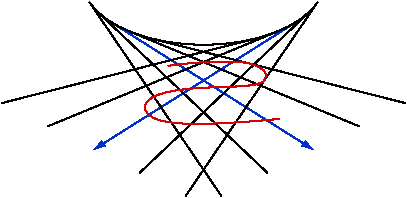
\includegraphics[height=1.93in]{main/Fig08-1}}\hfil
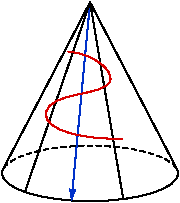
\includegraphics[height=2in]{main/Fig08-2}\quad}
\caption{Left: canonical curve of genus 4 on a smooth quadric, showing
  two $g^{1}_3$s.  Right: canonical curve of genus 4 on a quadric
  cone, with just one~$g^{1}_{3}$.}
\label{Fig8.1}
\end{figure}

Putting together
the analyses of the preceding sections, we have shown that
\index{hyperelliptic-trigonal dichotomy for curves of genus $\leq 4$}%
\emph{every curve of genus $g$ with $2\leq g \leq 4$ is either hyperelliptic or trigonal}.

\subsubsection*{Maps to $\PP^2$}

We can also describe the lowest degree plane models of nonhyperelliptic curves $C$ of genus 4.
We can get a plane model of degree 5 by projecting $C$ from a point $p$ of the canonical model of $C$.
Moreover, the
Riemann--Roch theorem
\index{Riemann--Roch theorem}%
shows that if $D$ is a divisor of
degree 5 with $r(D)=2$ then
$\h^0(K-D) = 1$. Thus $D$ is of the form
$K-p$ for some point $p \in C$, and the map to $\PP^2$ corresponding
to $D$ is $\pi_p$. These  maps $\pi_p: C\to \PP^2$ have the lowest
possible degree (except for those whose image is  contained in a line)
because by
Clifford's theorem
\index{Clifford's theorem}%
a nonhyperelliptic curve of genus 4
cannot have a $g^2_4$.

We now consider the singularities of the
plane quintic
\index{plane quintic}%
$\pi_p(C)$.
Suppose as above that $C = Q\cap S$, with $Q$ a quadric. If a line $L$
through $p$ meets $C$ in $p$ plus a divisor of degree $\geq 2$ then,
as we have seen, $L$ must lie in $Q$.  Any line through $p$ that is
not contained in $Q$ meets $C$ in at most a single reduced point,
whose image is thus a nonsingular point of $\pi(C)$. Moreover, a line
that met $C$ in a divisor of degree 4 or more
would have to lie in both the quadric and
the cubic containing $C$, and therefore would be contained in $C$.
Since $C$ is irreducible there can be no such line; thus the image
$\pi_p(C)$ has at most double points.

We distinguish two cases, depending on whether
the quadric $Q$ is smooth or singular. We will make use of the
Gauss map
\index{Gauss map}%
of the quadric,
described by the next lemma.

\begin{lemma}
Let $L \subset S \subset \PP^3$ be a line on a surface $S \subset \PP^3$ of degree $d \geq 2$, and
write $S_{\sing}$ for the singular locus of $S$. The Gauss map $\cG :
S \to (\PP^3)^*$ sending each point $p \in S\setminus S_{\sing}$ to
the tangent plane $\TT_p(S)$ maps $L$ into the
dual line
\index{dual line!def}%
in $\PP^3$ (that is, the locus of planes containing $L$); if $S$ is
smooth along $L$ then $\cG$  has degree $d-1$, and if $S$ is singular
anywhere along $L$ it has strictly lower degree.
\unif
\end{lemma}

The geometric idea behind this result is easy to understand: If $S$ is
smooth along $L$ and $H\cong \PP^{2}$ is a plane containing $L$, then
$H\cap S = L \cup D$ for a plane curve $D$ of degree $d-1$. The plane
$H$ is tangent to $S$ at a point $p$ if and only~if $H\cap S$ is
singular at $p$; and this occurs at each of the $d-1$ points (counted
with multiplicity) at which $D$ meets $L$, suggesting that the
restriction of the Gauss map is $(d{-}1)$-to-one in this case.

If $S$ is singular somewhere along $L$, then every plane through that point would be among the tangent
planes in the sense above, and the image of $L$ would be a component of a curve of degree $d-1$ containing a line; thus of lower degree.

To see that the multiplicities count correctly in this argument, we will give an algebraic version:
\unif

\begin{proof}
Suppose that in terms of homogeneous coordinates $[X,Y,Z,W]$ on $\PP^3$ the line $L$ is given by $X = Y = 0$. Then the defining equation $F$ of $S$ can be written
$$
F(X,Y,Z,W) = X\cdot G(Z,W) + Y\cdot H(Z,W) + J(X,Y,Z,W)
$$
where $J$ vanishes to order 2 along $L$; that is, $J \in (X,Y)^2` `$. The Gauss map $\cG|_L$ restricted to $L$ is then given by
$$
[0,0,Z,W] \mapsto [G(Z,W), H(Z,W), 0, 0].
$$
The polynomials $G$ and $H$ have degree $d-1$, and have a common zero if and only~if $S$ is singular somewhere along $L$; the lemma follows.
\end{proof}

\begin{example}[Gauss map of a quadric]
\label{Gauss of Quadric}
Let $Q\subset \PP^3$ be a smooth quadric,
\index{Gauss map!of a quadric}%
\index{quadric!Gauss map of}%
and let $L\subset Q$ be the line $X=Y =0$. Since we may write the
equation of $Q$ as $XZ+YW = 0$, the Gauss map of $Q$, restricted to
$L$, maps $L$ one-to-one onto the dual line. Indeed, the
Gauss map
takes $Q$ isomorphically onto its dual, which is also a smooth quadric.

 We can also see this geometrically: if $H \subset \PP^3$ is any plane containing the line $L \subset Q$, then $H$ intersects $Q$ in the union of $L$ and a line $M$; the hyperplane section $Q \cap H = L \cup M$ is then singular at a unique point $p \in L$. Thus the Gauss map gives a bijection between points on $L$ and planes containing $L$.
\unif
\end{example}

Given this, we can analyze the geometry of projections $\pi_p(C)$ of our canonical curve $C = Q \cap S$ as follows:

\begin{enumerate}
\item $Q$ is nonsingular:
In this case there are two lines $L_1, L_2$ on $Q$ that pass through
$p$; they meet $C$ in $p$ plus divisors $E_1$ and $E_2$ of degree 2.
If each $E_i$ consists of distinct points then, since the tangent
planes to the quadric along $L_i$ are all distinct by
Example~\ref{Gauss of Quadric}, the plane curve $\pi(C)$ has two
nodes, one at the image of each $E_i$.

On the other hand, if $E_i$ consists of a double point $2q$ (that is,
$L_i$ is tangent to $C$ at $q\neq p$, or meets $C$ three times at
$q=p$), then $\pi(C)$ has a cusp at the corresponding image point.

In either case, $\pi(C)$ has two distinct singular points, each either a
node or a cusp. The two $g^1_3$s on $C$ correspond to the
projections from these singular points. These possibilities are
illustrated in Figure~\ref{Fig8.2A}.

\begin{figure}[b]
\centerline {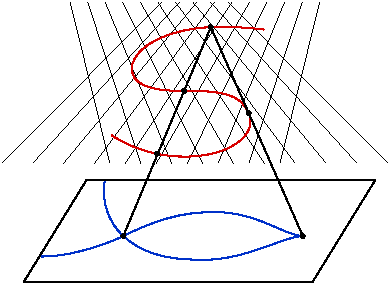
\includegraphics[height=2in]{main/canonical-projected-2}}
\caption{If a genus 4 canonical curve $C$ lies on a smooth quadric, the image of the projection of $C$ from a point $p\in C$
is a
plane quintic
\index{quintic!plane}%
with two singular points.
\hbox to 50pt{} % avoid extra jump before short line
}
\label{Fig8.2A}
\end{figure}

\item $Q$ is a
cone:
\index{cone quadric}%
In this case, since the curve cannot pass through the singular point
of $Q$ there is a unique line $L\subset Q$ that passes through $p$.
Let $p+E$ be the divisor on $C$ in which this line meets $C$. The
tangent planes to $Q$ along $L$ are all the same. Thus if
$E = q_1+q_2$ consists of two distinct points,
the image $\pi_p(C)$ has two smooth branches sharing a common tangent line at
$\pi_p(q_1) = \pi_p(q_2)$. Such a point is called a \emph{tacnode}
(Figure \ref{simplesing})
\index{tacnode}%
of $\pi_p(C)$. On the other hand, if $E= 2q$, that is, if $L$ meets $C$
tangentially at one point $q\neq p$ (or meets $C$ three times at $p$) then
the image curve has a higher-order cusp, called a \emph{ramphoid}
(``beak-like'')
\emph{cusp}
(Figure \ref{ramphoid}).
\index{ramphoid}%
\index{cusp!ramphoid}%
In either case, the one $g^1_3$ on $C$ is the projection from the
unique singular point of $\pi(C)$.
\end{enumerate}

\begin{figure}
\includegraphics[height=1.3in]{"main/ramphoid"}
\caption{A ramphoid cusp on a quartic curve with affine parametrization
$(t^2{+}t^3,t^4)$. Note that the real points of this affine curve lie
entirely in one of the half-planes determined by the tangent line
at the cusp. This was first recorded in a 1744 letter from Leonhard Euler to
Gabriel Cramer,
who had conjectured that for an algebraic curve, the
tangent at a cusp always lies between the two branches.}
\index{Cramer, Gabriel}%
\index{Euler, Leonhard}%
\label{ramphoid}
\end{figure}
\index{genus 4|)}%

\section{Curves of genus 5}

We next consider a nonhyperelliptic curve $C$ of genus 5. There are
\index{genus 5!curve|(}%
now two questions that cannot be answered by simple application of the
Riemann--Roch
theorem:

\begin{enumerate}
\item Is $C$ expressible as a
3-sheeted cover
\index{3-sheeted cover!of $\PP\sp 1$}%
of $\PP^1$?
Equivalently,
does $C$ have a
$g^1_3$?%
\index{g@$g^1_3$}%
\item Is $C$ expressible as a
4-sheeted cover!of $\PP\sp 1$
of $\PP^1$?
In other words, does $C$ have a basepoint free
$g^1_4$?
\index{g@$g^1_4$}%
\end{enumerate}

The first question is answered in the negative by the dimension count
of Section~\ref{Hurwitz spaces}, but the analysis below will give us a
way of characterizing those curves of genus 5 that are trigonal. Note
also that if a curve $C$ of genus 5 is trigonal, the $g^1_3$ on $C$ is
unique: if there were two distinct $g^1_3$s on $C$, with associated
maps $\alpha, \beta : C \to \PP^1` `$, the product map
$$
\alpha \times \beta : C \to \PP^1 \times \PP^1
$$
would give a
birational
\index{birational}%
embedding of $C$ as a curve of
bidegree $(3,3)$
\index{bidegree!$(3,3)$}%
in $\PP^1 \times \PP^1` `$, and it would follow from the genus formula
for curves on $\PP^1 \times \PP^1$ that the genus of $C$ would be at most 4.
\index{P^1 x P^1@$\PP^1 \times \PP^1$|see bidegree}%

The argument of the preceding paragraph can be applied more broadly,
and it's worth stating the results here:

\begin{proposition}\label{general gonality exclusion}
Let $d$ and $e$ be relatively prime integers. If $C$ is a curve of genus $g$ with a basepoint free $g^1_d$ and a basepoint free $g^1_e$, then
$$
g \leq (d-1)(e-1).
$$
The same conclusion holds when $C$ has two distinct
$g^1_d$s with $d$ prime.
\index{g@$g^1_d$, $d$ prime}%
\end{proposition}

\begin{proof}
As before, we let $\alpha$ and $\beta : C \to \PP^1$ be the maps
associated to the $g^1_d$ and the $g^1_e$. In either case
the
product map $\alpha \times \beta : C \to \PP^1 \times \PP^1$ is a
birational embedding of $C$ as a curve of bidegree $(d,e)$ in $\PP^1
\times \PP^1` `$, and the result follows.
\end{proof}


The condition of (relative) primeness is necessary: if $d=ma$ and
$e=mb$, the map $\alpha \times \beta : C \to \PP^1 \times \PP^1$ could
express $C$ as an $m$-sheeted cover of a curve $C_0 \subset \PP^1
\times \PP^1$ of bidegree $(a,b)$, and the genus of $C$ could be
arbitrarily large.

See Exercise~\ref{curve in a product} for the corresponding inequality
where the target curves have higher genus.

\index{genus 5!curve|)}%

\section{Canonical curves of genus 5}

As in the  case of genus 4, the answers to the basic questions above
about linear series on a curve $C$ of genus 5 can be found through an
investigation of the geometry of the canonical model $C \subset \PP^4$
of $C$. This is an
octic curve
\index{octic curve!in $\PP^4$}%
in $\PP^4` `$, and as before the first
question to ask is what sort of polynomial equations define $C$. We
start with quadrics, by considering the restriction map
\index{genus 5!canonical curves|(}%
$$
\rho_2 : H^0(\cO_{\PP^4}(2)) \; \to \; H^0(\cO_{C}(2)).
$$
On the left, we have the space of homogeneous quadratic polynomials on
$\PP^4` `$, which has dimension $\tbinom{6}{4} = 15$, while by the
Riemann--Roch theorem
\index{Riemann--Roch theorem}%
the target is a vector space of dimension
$$
2\cdot8 - 5 + 1 = 12.
$$
We deduce that $C$ lies on at least 3 independent quadrics. (We will
see in the course of the following analysis that it is exactly 3; that
is, $\rho_2$ is surjective.) Since $C$ is irreducible and, by
construction, does not lie on a hyperplane, each of the quadrics
containing $C$ is irreducible, and thus the intersection of any two is
a surface of degree 4. There are now two possibilities:  The
intersection of (some) three independent  quadrics $Q_1 \cap Q_2 \cap
Q_3$ containing the curve is 1-dimensional; or every such intersection
is 2-dimensional.

\subsection*{First case: the intersection of the quadrics is one-dimensional}
%\label{nontrigonal genus 5}
  By
B\'ezout's theorem
\index{B\'ezout's theorem}%
the intersection is a curve of
degree 8, and since $C$ also has degree 8 we must have
$C=Q_1 \cap Q_2 \cap Q_3$; that is, the canonical curve is a
complete intersection.
\index{complete intersection of three quadrics}%
Lasker's theorem
\index{Lasker's theorem}%
then shows that the three quadrics
generate the
whole homogeneous ideal of $C$; in particular, there are no additional
quadrics containing $C$.

We can now answer the first of our two questions for curves of this
type. As in the genus 4 case the geometric Riemann--Roch theorem
\index{Riemann--Roch theorem!geometric}%
implies that $C$ has a $g^1_3$ if and only~if the canonical model of
$C$ contains 3 collinear points or, more generally, meets a line $L$
in a divisor of degree 3 (Figure~\ref{3 collinear points from g13}).
When $C$ is the intersection of quadrics, this cannot happen, since
the line $L$ would have to be contained in all the quadrics that
contain $C$. Thus, in this case,
$C$ has no $g^1_3$.

\begin{figure}
\centerline {\includegraphics[width=3.6in]{"main/Fig08-5"}}
\caption{If $C$ has a $g^{1}_{3}$ then, in the canonical embedding, the three
points
of each divisor are collinear, and the lines they span sweep out a surface.
}
\label{3 collinear points from g13}
\end{figure}


What about $g^1_4$s? Again invoking the geometric Riemann--Roch
\index{Riemann--Roch theorem!geometric}%
theorem, a divisor of degree 4 moving in a pencil lies in a 2-plane;
so the question is, does $C \subset \PP^4$ contain a divisor of degree
4, say $D = p_1+\dots +p_4 \subset C$, that lies in a plane $\Lambda$?
Supposing this is so, we consider the restriction map
$$
H^0(\cI_{C/\PP^4}(2)) \; \to \; H^0(\cI_{D/\Lambda}(2)).
$$
By what we have said, the left-hand space is 3-dimensional.
We will show that the right-hand space
is 2-dimensional, so that one of the quadrics vanishes identically on $\Lambda$.

\begin{lemma}\label{4-tuples}
Let $\Gamma \subset \PP^2$ be any scheme of dimension $0$ and degree
$4$. Either $\Gamma$ is contained in a line $L \subset \PP^2` `$, or
$\Gamma$ imposes
independent conditions on quadrics,
\index{independent conditions!by four points, on quadrics}%
that is,
$h^0(\cI_{\Gamma /\PP^2}(2)) = 2$.
\end{lemma}

\begin{proof}
We will do this in case $\Gamma$ is reduced, that is, consists of four distinct points; the reader is asked to supply the analogous argument in the general case in Exercise~\ref{nonred 4-tuples}. Suppose to begin with that $\Gamma$ fails to impose independent conditions on quadrics, and let $q \in \PP^2$ be a general point. Since we are assuming that $h^0(\cI_{\Gamma /\PP^2}(2)) \geq 3$, we see that there are at least two conics $C', C'' \subset \PP^2$ containing $\Gamma \cup \{q\}$. By B\'ezout's theorem, these two conics have a component in common, which can only be a line $L$; thus we can write $C' = L \cup L'$ and $C'' = L \cup L''$ for some pair of distinct lines $L', L'' \subset \PP^2` `$. The intersection $C' \cap C''$ thus consists of the line $L$ and the single point $L' \cap L''$. Since this must contain $\Gamma \cup \{q\}$, and $q$ does not lie on the line joining any two points of $\Gamma$, we conclude that $L' \cap L'' = \{q\}$ and hence $\Gamma \subset L$.
%\vspace*{-12pt}
\end{proof}

\begin{fact}
Lemma~\ref{4-tuples} is the first case of a more general statement: If~
$n\leq 2d+1$ points in the plane fail to impose independent conditions
\index{independent conditions}%
on forms of degree $d$, then $d+2$ of the points lie on a line. See
\cite[p.~302]{MR1376653} for a proof.
\end{fact}


 It follows that the 2-plane $\Lambda$ spanned by $D$ must be contained in one of the quadrics $Q \subset \PP^4$ containing $C$. This implies in particular that the quadric is singular: If $V = \CC^3\subset \CC^5$
is a  3-dimensional subspace of a 5-dimensional inner-product space, then $V$ meets its orthogonal space
in a line, which is a singular point of the corresponding quadric.

Thus $Q$ is a
cone over a quadric
\index{cone!over a quadric surface}%
in $\PP^3` `$, and it is ruled by
the (one or two) families of 2-planes it contains, which are the cones
over the (one or two) rulings of the quadric in $\PP^3` `$. The
argument above shows that the existence of a $g_4^1$s on $C$ in this
case implies the existence of a singular quadric containing $C$.

Conversely, suppose that $Q \subset \PP^4$ is a
singular quadric
\index{quadric! in $\PP^4$, singular}%
containing $C = Q_1 \cap Q_2 \cap Q_3$. Now say $\Lambda \subset Q$ is
a 2-plane. If $Q'$ and $Q''$ are quadrics that with $Q$ span the
space of quadrics containing $C$, then we can write
$$
\Lambda \cap C = \Lambda \cap Q' \cap Q'',
$$
from which we see that $D = \Lambda \cap C$ is a divisor of degree 4
on $C$, and so has $r(D) = 1$ by the geometric Riemann--Roch theorem.
\index{Riemann--Roch theorem!geometric}%
Thus, the rulings of  singular quadrics containing $C$ cut out on $C$
pencils of degree 4; and every pencil of degree 4 on $C$ arises in
this way.

Does $C$ lie on singular quadrics? There is a $\PP^2$ of quadrics
containing $C$\emdash a 2-plane in the space $\PP^{14}$ of quadrics in
$\PP^4$\emdash and the family of singular quadrics  consists of a
hypersurface of degree 5
\index{quintic!hypersurface}%
in $\PP^{14}$, called the
\emph{discriminant}
\index{discriminant}%
\index{Bertini's theorem}%
hypersurface. By
Bertini's theorem,
not every quadric containing $C$
is singular. Thus the set of singular quadrics containing $C$ is a
plane curve $B$ cut out by a
quintic equation.
\index{quintic equation}%
So $C$ does indeed have
a $g^1_4$, and is expressible as a
\index{4-sheeted cover!of $\PP^1$}%
4-sheeted cover of~$\PP^1` `$.
Each singular quadric contributes either
one or two
$g^1_4$s, depending on
whether it has rank 3 or 4. In sum, we have proven:

\begin{proposition}
Let $C \subset \PP^4$ be a canonical curve, and assume $C$ is the
complete intersection of three quadrics
\index{complete intersection!of three quadrics}%
in $\PP^4` `$. Then $C$ may be
expressed as a 4-sheeted cover of $\PP^1$ in a one-dimensional family
of ways, and there is a map from the set
$W^1_4(C)$
\index{W@$W^1_4$}%
of $g^1_4$s on $C$
to a plane quintic curve $B$, whose fibers have cardinality $1$ or $2$.
\unif
\end{proposition}

One can go further and ask about the geometry of the plane curve $B$
and how it relates to the geometry of $C$. The list of possibilities
is given in \cite[p.~274]{ACGH}.
%\fix{possibly include a photo here?}

\subsection*{Second case: the intersection of the quadrics is a surface}
\label{trigonal genus 5} % for page number

We will show that the intersection must contain an irreducible,
nondegenerate surface. This  follows from
Fulton's
{\it elementary B\'ezout theorem}:
\index{Fulton, William}%
\index{Fulton's elementary B\'ezout theorem}%
\index{elementary B\'ezout theorem}%
\index{B\'ezout theorem!elementary}%

\begin{npt}
\begin{theorem}[\cite{Fulton}]
\label{Fulton Bezout}
Let $Z_1,\dots, Z_k \subset \PP^n$ be hypersurfaces of degrees $d_1,\dots,d_k$. If $\Gamma_1,\dots,\Gamma_m$ are the irreducible components of the intersection $\lessbigcap_1^kZ_j$, then
$$
\let\;\,
\sum_{\alpha = 1}^m \deg \Gamma_\alpha \; \leq \; \prod_{i=1}^k d_i.
$$
\end{theorem}
\end{npt}

\begin{proof}
We
use
induction on $k$, the result being trivial for $k=1$. Assuming that the result
is true for $k-1$, we consider the irreducible components $V_i$ of $\lessbigcap_1^{k-1}Z_j$. If $Z_k$ contains
$V_i$, then $V_i$ is again a component of $\lessbigcap_1^kZ_j$. Otherwise,
$V_i\cap Z_k$ is a union of components whose degrees sum to $d_k\deg V_i$. Thus
the sum of the degrees of the components of $\lessbigcap_1^kZ_j$ is at most $d_i$ times the
sum of the degrees of components of $\lessbigcap_1^{k-1}Z_j$, as required.
\meshing
\end{proof}

Returning to the canonical curve $C \subset \PP^4` `$, suppose that
the intersection $X = Q_1 \cap Q_2 \cap Q_3$ of the three quadrics
containing $C$ has dimension 2. If $C$ were a component of~$X$, then
the sum of the degrees of the irreducible components of $X$ would be
strictly greater than 8, which Fulton's theorem doesn't allow. Thus
$C$ must be contained in a 2-dimensional irreducible component  $S$ of
$X$, and this surface $S$ is necessarily nondegenerate.

We will return to this surface in Chapter~\ref{ScrollsChapter},
where we develop the theory of rational normal scrolls.
Here is the result:

\begin{theorem}
Let $C \subset \PP^4$ be a canonical curve of genus 5.
\index{canonical curve!of genus 5}%
\index{genus 5!canonical curve}%
Then $C$ lies on exactly three quadrics, and either
\begin{enumerate}
\item $C$ is the intersection of these quadrics; in which case $C$ is
  not trigonal, and the variety $W^1_4(C)$ of expressions of $C$ as a
  4-sheeted cover of $\PP^1$ is a 2-sheeted cover of a plane quintic
  curve; or
\item the quadrics containing $C$ intersect in a cubic surface that is
a nonsingular rational normal scroll; in this case, $C$ has a unique
$g^1_3$, and the variety
$W^1_4(C)$
\index{W@$W^1_4$}%
consists of the union of two
copies of $C$ meeting at two points.
\unif
\end{enumerate}
\end{theorem}

\begin{fact}
In the second case of the theorem, the ideal of the curve has the form $I_C = (Q_1, Q_2, Q_3, F_1, F_2)$
where the $Q_i$ are quadrics and the $F_i$ are cubic forms.
The quadrics $Q_i$ cut out a surface
scroll,
\index{scroll}%
which
must be smooth by Corollary~\ref{curves on a singular scroll}.

There are 2 linear relations among the
$Q_i$, and we shall see in Chapter~\ref{SyzygiesChapter}
that this is a special case of the
Eagon--Northcott complex.
\index{Eagon--Northcott complex}%
The generators of $I_C$ above may be written as the $4\times 4$
Pfaffians
\index{Pfaffian}%
of a skew-symmetric $5\times 5$ matrix of the form
$$
\begin{pmatrix}
0&g_1&g_2&\ell_0&\ell_1\\
-g_1&0&g_3&\ell_2&\ell_3\\
-g_2&-g_3&0 &\ell_3&\ell_4\\
-\ell_0&-\ell_2&-\ell_3&0&0\\
-\ell_1&-\ell_3&-\ell_4&0&0
\end{pmatrix}
$$
where $\ell_0,\dots,\ell_3$ are linear forms and $g_1, g_2, g_3$ are quadrics. The
 $2\times 2$
minors of the matrix of linear forms in the last two columns are the three quadrics $Q_i$ contained in the ideal
of $C$, and those two columns are the linear relations on the $Q_i$ mentioned above.
The columns of the whole $5\times 5$ matrix generate the syzygies of $I_C$. Moreover, the
$4\times 4$ Pfaffians of any sufficiently general matrix of this form define a
trigonal canonical curve;
\index{trigonal!canonical curve}%
see \cite{MR453723}.
\index{genus 5!canonical curves|)}%
\end{fact}

\section{Exercises}

\begin{exercise} \label{ex7.1}
Let $C$ be a smooth projective nonhyperelliptic
curve of genus 4,
\index{genus 4!curve}%
and $|D|$ a $g^1_3$ on $C$. Show that the following are equivalent:
\begin{enumerate}
\item $D \sim K-D$.
\item The multiplication map $\mu \,{:}\, H^0(D) \otimes H^0(K-D) \to H^0(K)$ fails to be sur\-jec\-tive.
\item The unique quadric $Q$ containing the canonical curve of $C$ is singular.
\item $|D|$ is the unique $g^1_3$ on $C$.
\end{enumerate}

Hint: Recall that the $g^1_3$s on $C$ are cut by the rulings of the quadric $Q$.
\end{exercise}

\begin{exercise}\label{ex7.2}
Let $C$ again be a smooth projective nonhyperelliptic curve of genus 4
whose canonical model lies on a smooth quadric. We have seen that $C$ is
birational
\index{birational}%
\index{genus 4!curve}%
to a
quintic plane curve
\index{quintic!plane curve}%
$C_0$ with two nodes $p, q \in
C_0$. Show that the canonical series of $C$ is cut out by the system
of plane conic curves passing through $p$ and $q$ in the sense
that if $D$ is a curve meeting $C$ at each node and transverse to each
branch at the nodes, then
the sum of the points of $D\cap C$ \emph{other than the nodes} is a canonical divisor.

Hint: Try
blowing up
\index{blowup}%
the plane at the nodes. Look at
Section~\ref{canonical series on nodal plane curves} if you get stuck.
\end{exercise}

\begin{exercise}\label{ex7.3}
Let $C$  be a smooth projective nonhyperelliptic curve of genus 4 and
let $D$ be a general divisor of degree 7 on $C$. By the
$g+3$ theorem
\index{g+3@$g+3$ theorem}%
(Theorem~\ref{g+3 theorem}), $h^0(D) = 4$ and the map $\phi_D : C \to
\PP^3$ is an embedding. Show that the image $C \subset \PP^3$ does not
lie on any quadric surfaces, but does lie on two cubic surfaces $S$
and $T$; describe the intersection $S \cap T$.

Hint: For the first part: if the curve $C \subset \PP^3$ lay on a quadric, what would be its class? For the second, if $S \cap T = C \cup D$, calculate the degree and genus of $D$ (see Chapter~\ref{LinkageChapter} if you get stuck).
\end{exercise}

\begin{exercise}\label{ex7.4}
We keep
the setting of the preceding exercise,
but now
suppose that $C$ \emph{is} hyperelliptic. Show that in this case the
image of $C$ under the map $\phi_D : C \to \PP^3$ does lie on a
quadric surface $Q$, and in fact is a curve of type $(2,5)$ on $Q$.
Show also that if $D$ is of the form $D \sim 2g^1_2 + p + q + r$ then
the quadric surface $Q$ is singular, and the image curve $\phi_D(C)$
has a triple point at the vertex of $Q$.

Hint: Show that each of the divisors $E$ of the $g^1_2$ span a line in $\PP^3` `$.
 \end{exercise}

\begin{exercise}\label{ex7.5}
Consider a space $M^r_{d,g}$ parametrizing $g^r_d$s on curves of genus $g$; that is,
$$
M^r_{d,g} = \{ (C, L) \mid C \text{ a smooth curve of genus } g, L \in \pic^d(C) \text{ and } h^0(L) \geq r+1 \}.
$$
The analysis of this chapter shows that
$M^1_{3,4}$
\index{M@$M^1_{3,4}$}%
is a
2-sheeted cover of $M_4$.
\index{2-sheeted cover!of $M_4$}%
Show that it is in fact irreducible.

Hint: Consider the incidence correspondence
$$
\Gamma \colonequals  \{ (Q, L) \in \PP^9 \times \GG(1,3) \mid L \subset Q \}
$$
where $\PP^9$ is the space of quadrics $Q\subset \PP^3` `$.
\end{exercise}

\begin{exercise}\label{ex7.6}
The arguments in the chapter show that the canonical model of a
nonhyperelliptic trigonal curve of genus 5 lies on an irreducible,
nondegenerate
cubic surface $S \subset \PP^4` `$.
\index{cubic surface!in $\PP^4$}%
Chapter~\ref{ScrollsChapter}, we'll see that such a surface is either
smooth or a cone over a twisted cubic curve. Show that the latter case
cannot occur.

Hint: By projection, show that $C$ would have to be double at the vertex of the cone.
\end{exercise}

\begin{exercise}\label{ex7.7}
Let $C$ be a smooth projective curve of genus 5. The
$g+3$ theorem
\index{g+3@$g+3$ theorem}%
(Theorem~\ref{g+3 theorem}) says that $C$ admits an embedding in
$\PP^3$ as a
curve of degree 8.
\index{octic curve}%
Does it admit an embedding of degree 7?

Hint: Show that the linear series $|K_C - p|$ is very ample if and only~if $C$ is not trigonal.
\end{exercise}

\begin{exercise}\label{nonred 4-tuples}\label{ex7.8}
Complete the proof of Lemma~\ref{4-tuples}.

Hint: Consider separately the cases where $\Gamma$ contains a
fat point
\index{fat point|defi}%
(that is, the scheme defined by the square of the maximal ideal at a
point) or is
curvilinear
\index{curvilinear|defi}%
(that is, has Zariski tangent space of
dimension at most 1 everywhere).
\end{exercise}

\input footer.tex

%header and footer for separate chapter files

\ifx\whole\undefined
\documentclass[12pt, leqno]{book}
\usepackage{graphicx}
\usepackage{eps-to-pdf}
\input style-for-curves.sty
%\input sl-macros.sty
\usepackage{hyperref}
\usepackage{showkeys} %This shows the labels.
\usepackage{msribib}
\usepackage{pdfpages}
\usepackage{draftwatermark}
\SetWatermarkText{DRAFT:\ \today}
\SetWatermarkScale{2}
\SetWatermarkColor[gray]{0.9}

%\usepackage{SLAG,msribib,local}
%\usepackage{amsmath,amscd,amsthm,amssymb,amsxtra,latexsym,epsfig,epic,graphics}
%\usepackage[matrix,arrow,curve]{xy}
%\usepackage{graphicx}
%\usepackage{diagrams}
%
%%\usepackage{amsrefs}
%%%%%%%%%%%%%%%%%%%%%%%%%%%%%%%%%%%%%%%%%%
%%\textwidth16cm
%%\textheight20cm
%%\topmargin-2cm
%\oddsidemargin.8cm
%\evensidemargin1cm
%
%%%%%%Definitions
%\input preamble.tex
%\input style-for-curves.sty
%\def\TU{{\bf U}}
%\def\AA{{\mathbb A}}
%\def\BB{{\mathbb B}}
%\def\CC{{\mathbb C}}
%\def\QQ{{\mathbb Q}}
%\def\RR{{\mathbb R}}
%\def\facet{{\bf facet}}
%\def\image{{\rm image}}
%\def\cE{{\cal E}}
%\def\cF{{\cal F}}
%\def\cG{{\cal G}}
%\def\cH{{\cal H}}
%\def\cHom{{{\cal H}om}}
%\def\h{{\rm h}}
% \def\bs{{Boij-S\"oderberg{} }}
%
%\makeatletter
%\def\Ddots{\mathinner{\mkern1mu\raise\p@
%\vbox{\kern7\p@\hbox{.}}\mkern2mu
%\raise4\p@\hbox{.}\mkern2mu\raise7\p@\hbox{.}\mkern1mu}}
%\makeatother

%%
%\pagestyle{myheadings}

%\input style-for-curves.tex
%\documentclass{cambridge7A}
%\usepackage{hatcher_revised} 
%\usepackage{3264}
   
\errorcontextlines=1000
%\usepackage{makeidx}
\let\see\relax
\usepackage{makeidx}
\makeindex
% \index{word} in the doc; \index{variety!algebraic} gives variety, algebraic
% PUT a % after each \index{***}

\overfullrule=5pt
\catcode`\@\active
\def@{\mskip1.5mu} %produce a small space in math with an @

\title{A Chapter from ``The Practice of Algebraic Curves"}
\author{\copyright David Eisenbud and Joe Harris}
%%\includeonly{%
%0-intro,01-ChowRingDogma,02-FirstExamples,03-Grassmannians,04-GeneralGrassmannians
%,05-VectorBundlesAndChernClasses,06-LinesOnHypersurfaces,07-SingularElementsOfLinearSeries,
%08-ParameterSpaces,
%bib
%}

\date{\today}
%%\date{}
%\title{Curves}
%%{\normalsize ***Preliminary Version***}} 
%\author{David Eisenbud and Joe Harris }
%
%\begin{document}

\begin{document}
\maketitle

\pagenumbering{roman}
\setcounter{page}{5}
%\begin{5}
%\end{5}
\pagenumbering{arabic}
\tableofcontents
\fi



\chapter[Hyperplane sections of a curve]{Hyperplane sections\\of a curve}
\label{linear general position chapter}

One way to study a curve in $\PP^r$ is to use properties of its hyperplane
sections. In this chapter, we will take up the question: if $C \subset
\PP^r$ is a reduced, irreducible and nondegenerate curve, what can we say
about the geometry of the points in the  hyperplane section 
$\Gamma = C \cap H$ of $C$, and what more can we say about a general hyperplane
section?

We prove and apply a result originally due to Castelnuovo,
\index{Castelnuovo, Guido}%
that every subset of $r$ points in a
general hyperplane section
\index{general hyperplane section}%
of $C$ spans the hyperplane; that is, any $r$
points of $\Gamma$ are linearly independent. 
Recall (from just before Proposition \ref{points on rnc}) that
in this situation 
the points 
are said to be
in \emph{linearly general position}.
\index{linearly general position}%
Castelnuovo's result
holds for smooth curves in 
arbitrary characteristic;
\index{positive characteristic}%
see
Exercise~\ref{strange curves} for
interesting counterexamples involving singular curves in positive
characteristic. 

This is followed by a series of applications,
including 
a
\index{Castelnuovo's theorem}%
famous theorem of Castelnuovo bounding the genus of a
curve in terms of its degree,
and, through that result, a proof that canonical curves and linearly
normal curves ``of high degree'' are arithmetically Cohen--Macaulay
\index{ACM}%
(Theorem~\ref{list of Castelnuovo curves}).

\marginpar{Needs to be restored to normal size}
{\footnotesize  % temporary -- avoids a weird TeX error in the very
                % short first paragraph of section 10.1
In Chapter~\ref{uniform position}, we will explain and prove a still
stronger general position result, which requires characteristic 0, and
give applications to the irreducibility of fiber products, to the Hilbert
functions of subsets of the
general hyperplane section, and to sums of linear series.

}

\section{Linearly general position}\label{linearly general position
section}
In this section we 
allow our algebraically closed ground field to
have arbitrary characteristic.

An irreducible and reduced curve
$C\subset \PP^r$ over an algebraically closed field, 
other than a
\index{strange curve|defi}%
line, is called \emph{strange} if
all the tangent lines at smooth points of $C$ meet in a point $p\in \PP^r``$. 
If this condition seems somewhat\dots\ strange, that may be because no
such curves exist in characteristic 0: if 
all the
tangent lines at smooth points of $C$ met in a point, then the projection
of $C$ from that point would have derivative 0 everywhere and hence be
constant. But strange curves do exist in 
positive
characteristic, albeit
\index{Samuel, Pierre}%
rarely: Pierre Samuel showed that the only \emph{smooth} curve that is
strange (in any characteristic) is the conic in 
characteristic 2;
\index{characteristic 2}%
a proof
is given in \cite[Theorem IV.3.9]{Hartshorne1977}. Without the smoothness
hypothesis there are more examples; see Exercise~\ref{strange curves}.



\begin{npt}
\begin{theorem}[{{\cite[Lemma 1.1]{Rathmann}}}]
\label{basic linear independence}\label{linear general position}
\index{Rathmann, J\"{u}rgen}%
Suppose that $n\geq 3$. If $C\subset \PP^r$ is a nondegenerate,
irreducible, reduced curve
that is not strange,
and $H$ is a general hyperplane, then any $r$ points of $H\cap C$ are
linearly independent.
\unif
\end{theorem}
\end{npt}

We postpone the proof to introduce some related definitions.

For example, the theorem says that for $C \subset \PP^3` `$, the general
hyperplane section does not contain a line
\index{multisecant}%
that meets $C$ three or more times\emdash a \emph{multisecant}. Another
special configuration which is not present in a general hyperplane
section, as it turns out,
is any pair of points $p\neq q$ on $C$ such that the tangent lines
to $C$ at $p$ and $q$ intersect\emdash what was
classically
\index{stationary secant}%
called a 
\textit{stationary secant}
(Figure~\ref{Fig9.1}).

\begin{figure}
\vskip-3pt
\includegraphics[height=1.1in,angle=-20]{main/cradle-good}
\vskip-22pt
\caption{The lines $bd$ and $ae$ are stationary secants to a degree
  four space curve in red, because the tangents at $b$ and $d$
  have a nontrivial intersection, as do (at infinity) the tangents at
  $a$ and $e$.}
\label{Fig9.1}
\end{figure}

More formally we define two subsets of the symmetric square $C_2$ of $C$:
\index{mult|defi}%
\index{stat|defi}%
$$
\begin{aligned}
 \mult(C) &\colonequals \{@(p,q) \in C_2 \mid \overlw20{pq} \hbox{ meets
 $C$ in a scheme of length $\geq 3$}@\},\\
\stat(C) &\colonequals  \{@(p,q) \in C_2\setminus \Delta \mid  \hbox{the
tangent lines to $C$ at $p,q$ meet}
@\}.
\end{aligned}
$$
Here
$\overlw20{pq}$ 
denotes the secant line through $p,q$ (or the
tangent line if $p=q$) and $\Delta\subset C_2$
is the diagonal.


Clearly if $C$ is strange or planar then $\stat(C) = C_2\setminus \Delta$, 
and
if $C$ is
planar with $\deg C>2$ then $\mult(C) = C_2$.
These are the only such cases:

\begin{proposition}\label{mult and stat}
 If $C\subset \PP^r$ is a reduced, irreducible, curve that is neither
 planar nor strange, then $\mult(C)\subset C_2$
 and $\stat(C)\subset C_2\setminus \Delta$ are closed subsets of dimension
at most
 $1$.
\unif
\end{proposition}

\begin{proof}
To show that $\mult(C)$ is closed, consider the projection map
$$
\{((p,q), r) \in C_2\times \PP^r \mid r \in \overlw20{pq}@\} \to C_2
$$
sending  $((p,q),r)$ to $(p,q)$. By the 
semicontinuity of the degree
\index{semicontinuity of degree}%
in proper families of constant fiber dimension, the set of points lying
in fibers
of length $\geq 3$ is closed, and $\mult(C)$ is the image of this
set. Because the map is finite,
$\mult(C)$  is closed as well.

Similarly, since
$
\{((p,q), r) \in (C_2\setminus \Delta)\times \PP^r \mid r \in {\mathbb T}_p(C)\cup
{\mathbb T}_q(C) \}
$
is closed in $(C_2\setminus \Delta)\times \PP^r` `$, its image under
the projection to the first factor,
which is $\stat(C)$, is closed in $C_2\setminus \Delta$.

Suppose, contrary to the proposition, that $\dim \stat(C) >1$. Since
$\stat(C)$ is a closed subset of the irreducible variety $C_2\setminus
\Delta$ it
follows that $\stat(C) = C_2\setminus \Delta$, so every pair of tangent
lines meet. Any three
lines in projective space that meet pairwise must be either coplanar or
meet in a point. Thus if $C$ is not strange,
then all the tangents to $C$ lie in a common plane, and $C$ is planar,
contradicting our hypothesis
and proving that $\dim \stat(C)\leq 1$.

Finally suppose, contrary to the proposition,  that $\dim \mult(C)>1$. As
in the previous argument, this
implies that every secant is a multisecant.  We will show in this case
that $\dim \stat(C) =2$, a contradiction.

To this end, consider the projections $\pi_{p}: C \to \PP^{r-1}$ and
the set
$$
\tabcolsep1pt
I = \Bigl\{(p,r,r') \in C^3 \Bigm|
\begin{tabular}{l}\small $p,r,r'$ are distinct and\\[-2pt]
\small $\pi_{p}(r) = \pi_{p}(r')$ is a smooth point of $\pi_p(C)$
\end{tabular}
\Bigr\}.
$$
The tangent lines ${\mathbb T}_r(C)$ and ${\mathbb T}_{r'}(C)$ both project from $p$ to the
tangent line ${\mathbb T}_{\pi_p(r)}(\pi_C)$,
and thus they lie in the 2-plane spanned by $p$ and this line; it follows
that $(r,r') \in \stat(C)$.
The projection $I \to C_2: (p,r,r') \mapsto (r,r')$ is finite since the
secant line $\overkern10{rr'}$ meets $C$ in only finitely many points,
so $\dim I \leq \dim \stat(C)$.

 If the projection from some point $p$ were everywhere ramified,
then all tangents to $C$ would pass through $p$, and $C$ would be strange.
Since also every secant to $C$ is a multisecant it follows that  for
every smooth point $p\in C$ there is an open set of points $q\in \pi_p(C)$
such that
the fiber $\pi_p^{-1}(q)$ contains two distinct points of $C$. Thus the
projection $I \to C: (p,r,r') \mapsto p$ maps
$I$ onto an open set of $C$, with 1-dimensional fibers, so $2 = \dim
I\leq \dim \stat(C)$ as claimed. 
\end{proof}


\begin{proof}[Proof of Theorem~\ref{linear general position}]
If
$C\subset \PP^n$ is a reduced curve then, by Bertini's theorem, a general
\index{Bertini's theorem}%
hyperplane meets $C$ transversely.
First suppose that $n=3$, and consider the incidence correspondence
$$
I \colonequals  \{ ((p,q), H) \in \mult(C) \times (\PP^3)^* \mid
\overlw20{pq}\in H\}.
$$
Since $\dim \overlw20{pq} = 1$, the fibers of the projection of $I$
to $\mult(C)$ have dimension 1,
so $\dim I = 1+\dim \mult(C)  \leq 2$. Consequently the image of  the
projection of $I$ to $(\PP^3)^*$ has
dimension $\leq 2$, so there is an open set of planes that contain no
multisecants, proving the theorem in this case.

\begin{fact}
 Since a secant line to a curve $C$ that is not itself a line is
 determined by its intersections with $C$,
 every curve other than a line has a 2-parameter family of secant
 lines. If $C\subset \PP^3$ is nondegenerate,
 this means that it is 2 conditions for a line in $\PP^3$ to be a secant
 to $C$. Since a pencil of lines meets
 $C$ in codimension 1, one might expect that, correspondingly, there
 would be a 1-parameter family
 of trisecant lines and a finite number of 4-secant lines. One can
 compute the expected number enumeratively
 \cite[p.~296]{Griffiths-Harris1978}.
 For example a general curve of degree $\leq 4$ can have no 4-secant
 line (it would meet planes containing that line in at least 5 points),
 but a general rational curve of degree 5 in $\PP^3$
  has exactly 1 \cite[Section 12.4.4]{3264}. See  Figure~\ref{9.2}
  for a construction in which the 4-secant line is visible.

\begin{figure}[b]
\centerline {\includegraphics[height=1.5in]{"main/Fig09-2"}}
\caption{A smooth rational quintic in $\PP^{3}$ with a unique 4-fold
secant line
can be obtained as the image of a plane conic $C$ by the rational map
of $\PP^{2}$ to $\PP^{3}$
induced by the 4 cubics through 6 points $e_{1},\dots e_{6}$, exactly
one of which lies on $C$; the image of the unique conic $D$ through the
other 5 points becomes the 4-secant line to the image of $C$.
\marginparhere{\hsize=2\hsize\redden{You had a note to make the two conics different colors but I'm not sure why that's desirable; I'll comply if your confirm}}
}
\label{9.2}
\end{figure}

 This fact entered history in a peculiar way:
 After Kronecker \citeyear{Kronecker} proved that every algebraic set in
  $\PP^{n}$ is set-theoretically the intersection of $n+1$
\index{Vahlen, Karl Theodor}%
\index{Kronecker, Leopold}%
\index{set-theoretic equality}%
\index{quintic!rational}%
  hypersurfaces, 
Vahlen \citeyear{Vahlen} claimed that Kronecker's result was
  sharp ``because'' a general 
rational quintic
\index{historical context}%
with one 4-secant line
  could not be the intersection of 3 hypersurfaces.
  Vahlen played a role in the rise of the Nazi party, and perhaps for
  that reason 
Perron \citeyear{Perron} produced 3 hypersurfaces intersecting
\index{Perron, Oskar}%
  precisely in a given general rational quintic. It is now known that
  every algebraic set in
  $\PP^{n}$ over an infinite field can be written set-theoretically as
  the intersection of just $n$ hypersurfaces \cite{Eisenbud-Evans}.
\end{fact}

We next do induction on $n\geq 4$. We will show first that the image
$C'$ of
$C$ under the projection $\pi_p: C\to C'$ from a general point of $C$
is not strange. Since $C\subset \PP^r$ is neither
planar nor strange
Proposition~\ref{mult and stat} shows that we may choose two smooth points
$r,r'\in C\subset \PP^r$ such that ${\mathbb T}_r(C)\cap {\mathbb T}_{r'}(C) = \emptyset$,
and thus
${\mathbb T}_r(C)$ and ${\mathbb T}_{r'}(C)$ together span a 3-plane $L$. Since $C$ is
nondegenerate we may
choose a point $p\in C$ outside $L$, and it follows that $\pi_p$
restricted to $L$ is an isomorphism.
Thus ${\mathbb T}_{\pi_p(r)}(C') \cap {\mathbb T}_{\pi_p({r'})}(C') = \emptyset$, so $C'$
is not strange,
and since $n\geq 4$ the curve $C'$ is not planar either.

Arguing by contradiction, suppose that the general hyperplane section
of~$C$ contains a set of $r$ linearly dependent points. Consider the
closed subsets
$$
I_1 \subset I \subset \{@(p,H) \in C \times (\PP^n)^*@\}
,
$$
where $I$ is defined by the 
condition
that $p\in H$ and $I_1$ is defined
by the condition that, in addition, there exist $p_2,\dots, p_r\in H$
such that $p, p_2, \dots, p_r$ are dependent. Both $I_1$ and $I$ are
closed subsets.

By hypothesis, both $I_1$ and $I$ project onto open sets of $(\PP^n)^*$,
so they have the same dimension.
But $I$ is irreducible: it projects onto an open subset of $C$ with
fibers isomorphic to $\PP^{r-1}$. Thus $I_1 = I$,
and  $p$ is part of a dependent set
$\{p, p_2,\dots, p_r\}$ in a general hyperplane containing $p$.

Let $H'$ be a general hyperplane in $\PP^{n-1}$
and let $H = \pi_p^{-1}(H')$, which is a general hyperplane containing
$p$. The intersection $H\cap C$
contains $r$ dependent points $\{p, p_2,\dots, p_r\}$, and it follows
that $\pi_p(p_2),\dots,\pi_p(p_n)$
are dependent points of $H'\cap C'$. This contradicts the induction
hypothesis, and proves that
the general hyperplane section of $C$ is in linearly general position.
\end{proof}

 \section{Castelnuovo's theorem}\label{CastelnuovoSection}

Clifford's theorem gives a complete and sharp answer to the question,
\index{Castelnuovo's theorem}%
``what linear series can exist on a curve of genus $g$?''
But maybe that wasn't the question we meant to ask! After all, we're
interested in describing curves in projective space as images of abstract
curves $C$ under maps given by linear systems on $C$. Observing that
the linear series that achieve equality in 
Clifford's theorem
\index{Clifford's theorem}%
give maps of degree 2 onto a rational curve,
 we might hope that we
would have a 
 different and more relevant
answer if we
restrict our attention to linear series $\cD = (\cL,V)$ for which the
\index{birational}%
associated map $\phi_\cD$ is at least  birational onto its image.

A classical result of Castelnuovo does exactly that: it gives a sharp
bound on the 
arithmetic genus
\index{arithmetic genus}%
of a reduced, irreducible, nondegenerate
curve of degree $d$ in $\PP^r` `$. To state it, for positive integers $d$
and $r$, let
\index{M@$M=M(d,r)$|defi}%
\label{def of M}
$$
 M \colonequals  
M(d,r)
\colonequals  
\biggl\lfloor\mfrac{d-1}{r-1}\biggr\rfloor,
$$
so that
$$
 d -1 = M(r-1) + \epsilon
$$ 
for some $\epsilon = 
\epsilon(d,r)
$
 with $0 \leq \epsilon \leq r-2$.
\index{epsilon@$\epsilon=\epsilon(d,r)$|defi}%

\begin{theorem}[Castelnuovo's bound]\label{Castelnuovo's bound}
Let $C \subset \PP^r$ be a reduced, irreducible, nondegenerate curve of
\index{Castelnuovo's bound}%
degree $d$. With $M$ and $\epsilon$ defined
as above,
$$
p_a(C) \leq \pi(d,r) \colonequals  \frac{M(M-1)}{2}(r-1) + M\epsilon.
$$
Moreover, if $p_a(C) = \pi(d,r)$  then $C$ is arithmetically
\index{ACM}%
Cohen--Macaulay and every hyperplane
section $H\cap C$ has 
Hilbert function
\index{Hilbert function}%
$
\dim (R_{H\cap C})_{m} = \min\{m(r-1), d\}.
$
\end{theorem}

We will say that a curve achieving the bound is a \emph{Castelnuovo
\index{Castelnuovo curve}%
curve}.

\subsection*{Proof of Castelnuovo's bound}

The idea of Castelnuovo's proof is simple and beautiful. To start
with, the hypothesis that $C$ is nondegenerate in $\PP^r$ says that
$h^0(\cO_C(1)) \geq r+1$. We'd like to use this and the Riemann--Roch
formula, in the form
$$
g = d+1 - h^0(\cO_C(1)) + h^1(\cO_C(1)),
$$
but this doesn't work because we have a priori no way to estimate
$h^1(\cO_C(1))$.

Castelnuovo's solution  is to derive lower bounds not just on
$h^0(\cO_C(1))$ but on $h^0(\cO_C(m))$ for all $m$; since we know that
$h^1(\cO_C(m)) = 0$ for large $m$, a lower bound on $h^0(\cO_C(m))$
for large $m$ will translate directly into an upper bound on~$g$.

How can we go about estimating $h^0(\cO_C(m))$? The answer is to
derive lower bounds on the successive differences $h^0(\cO_C(m)) -
h^0(\cO_C(m-1))$, by letting $\Gamma = C \cap H$ be a general hyperplane
section of $C$, and viewing $H^0(\cO_C(m-1))$ as the subspace of
$H^0(\cO_C(m))$ consisting of sections vanishing on $\Gamma$. The
estimates we get may seem crude\emdash not surprisingly, considering
how little we know about~$\Gamma$\emdash but remarkably, the bound we
ultimately derive on the genus of $C$ turns out to be sharp!

For the proof, the following definition will be convenient:

\begin{definition}
If $\sV = (V,\cL)$ is a linear system on a variety $X$ and $\Gamma$
is a subscheme then the \emph{number of conditions imposed by $\Gamma$
\index{number of conditions!imposed by subscheme on a linear system}%
on $\sV$} (that is, the number of 
independent linear conditions
\index{independent linear conditions}%
for a
section in $V$ to vanish
identically on $\Gamma$) is the dimension of the image of $V$ in
$H^0(\sL|_\Gamma) = H^0(\sL \otimes \sO_\Gamma)$; or, numerically,
$$
\dim V - \dim \left(V \cap H^0(\cL\otimes \cI_{\Gamma/X}) \right).
$$
\end{definition}

Thus, for example, if $\Gamma \subset \PP^r` `$, then the number of
conditions imposed by $\Gamma$ on $H^0(\cO_{\PP^r}(m))$ is the value
$h_\Gamma(m)$ of the Hilbert function of $\Gamma$ at $m$.
Note that in case $\Gamma$ is zero-dimensional, the number of conditions
imposed by $\Gamma$ on a linear system $V$ is necessarily less than or
equal to the degree $d$ of $\Gamma$; if it is equal we say that $\Gamma$
\emph{imposes independent conditions on $V$}.

\begin{proof}[Proof of Theorem~\ref{Castelnuovo's bound}]
Suppose that $C \subset \PP^r$ is an irreducible, nondegenerate curve. For
large $m$ we have
$h^{0}(\sO_{C}(m)) = md-p_{a}(C) +1$, so to bound the genus from above
we must
bound $h^{0}(\sO_{C}(m))$ from below.

Let $\Gamma = C@\cap@H$ be a general hyperplane section of $C$, and
let $V_m`\subset`H^0(\cO_C(m))$ be the linear series cut on $C$ by
hypersurfaces of degree $m$ in $\PP^r` `$, that is, the image of the
restriction map
$$
H^0(\cO_{\PP^r}(m)) \to H^0(\cO_C(m)).
$$
The number of  conditions imposed by $\Gamma$ on $V_m$ is the rank of
the restriction map
$\rho_m: V_m \to \sO_\Gamma(m)$.
 The number of conditions imposed by $\Gamma$ on $H^{0}(\sO_{C}(m))$
 is the
 rank of the restriction map from this potentially larger space, and
 thus is at least as large. This
 accounts for the inequality in the following:
{\advance\jot-2pt
\begin{align*}
h^0(\cO_C(m)) - h^0(\cO_C(m-1)) & = \text{\# of conditions imposed by
$\Gamma$ on $H^0(\cO_C(m))$}\\
&\geq \text{\# of conditions imposed by $\Gamma$ on $V_m$} \\
&= \text{\# of conditions imposed by $\Gamma$ on $H^0(\cO_{\PP^r}(m))$} \\
&= h_\Gamma(m).
\end{align*}}%
Replacing $m$ by $k$ in the display above and summing
over $k$, we obtain the lower bound
$$
h^0(\cO_C(m)) \geq \sum_{k=0}^m h_\Gamma(k).
$$

In order to bound the genus $C$ from above, we will bound the Hilbert
function of its hyperplane section $\Gamma$  from below; and for this,
we need to know something about the geometry of $\Gamma$. In fact, all
we need to know is Theorem~\ref{linear general position}, which says
that the points of $\Gamma$ are in 
linearly general position!
\index{linearly general position}%

\begin{proposition}\label{min hilb}
If $\Gamma \subset \PP^r$ is a collection of $d$ points in linearly
general position that span $\PP^r` `$, then
$$
h_\Gamma(m) \geq
@
\begin{tcases}
mr+1&\hbox{ if $m\leq M(d,r+1)$,}\\
\hfil d &\hbox{ otherwise.}
\end{tcases}
$$
\end{proposition}

One way to understand the bound $mr+1$ is to realize that if $\Gamma$
is any finite subscheme of a rational normal curve $C\subset\PP^r$
of degree $r$,
then $h_\Gamma(m) = \min\{\deg \Gamma,@ mr`+`1\}$ for every $m$
(Exercise~\ref{linear bound is sharp}).
  Thus the bound in Proposition~\ref{min hilb} is best possible.
On the other hand, sets of points on a rational normal curve are almost
the only sets for which the bound is sharp. See Figure~\ref{Fig9.3}
for an illustration.

\begin{figure}
\centerline {\includegraphics[height=1.5in]{"main/Fig09-3"}}
\caption{The case $d = 3\cdot 2+1$: the point $e_{7}$ imposes an additional
condition on the cubics (such as the union of the three lines shown)
passing through
$e_{1},\dots, e_{6}$.}
\label{Fig9.3}
\end{figure}

\begin{proof}
Suppose first that $d \geq mr+1$, and let $p_1,\dots,p_{mr+1} \in
\Gamma$ be any subset of $mr+1$ points. It suffices to show that
$\Gamma' = \{p_1,\dots,p_{mr+1}\}$ imposes independent conditions 
on
$H^0(\cO_{\PP^r}(m))$, that is, for any $p_i \in \Gamma'$ there is a
hypersurface $X \subset \PP^r$ of degree $m$ containing all the points
$p_1,\dots, \hat{p_i},\dots,p_{mr+1}$ but not containing~$p_i$.

To construct such an $X$, group the $mr$ points of $\Gamma' \setminus
\{p_i\}$ into $m$ subsets $\Gamma_k$ of cardinality $r$; each set
$\Gamma_k$ will span a hyperplane $H_k \subset \PP^r` `$, and we can
take $X = H_1 \cup \dots \cup H_m$.

In the case where $d<mr+1$, we add $mr+1-d$ general points; each one
imposes exactly one
additional condition on hypersurfaces of degree $m$.
\end{proof}


To complete the proof of Theorem~\ref{Castelnuovo's bound} we add up the
lower bounds in the proposition. To this end, let $C \subset \PP^r$ be
 an irreducible, nondegenerate curve of degree $d$, and  set
$M= M(d,r) = \bigl\lfloor{\frac{d-1}{r-1}}\bigr\rfloor$ 
as on page~\pageref{def of M}.
We have
\begin{align*}
h^0(\cO_C(M)) &= \sum_{k=0}^M h^0(\cO_C(k)) - h^0(\cO_C(k-1)) \\
&\geq  \sum_{k=0}^M (k(r-1)+1) 
= \frac{M(M+1)}{2}(r-1) + M + 1
,
\end{align*}
and similarly
$$
h^0(\cO_C(M+m)) \geq \frac{M(M+1)}{2}(r-1) + M  + md+ 1
.
$$
For sufficiently large $m$, the line bundle $\cO_C(M+m)$ is nonspecial,
so by the 
Riemann--Roch theorem,
\index{Riemann--Roch theorem}%
\begin{align*}
g &= (M+m)d - h^0(\cO_C(M+m)) + 1 \\
&\leq (M+m)d - \left(  \frac{M(M+1)}{2}(r-1) + M + 1 + md \right)+1 \\
& = M\bigl( M(r-1) + 1 + \epsilon \bigr) - \left(  \frac{M(M+1)}{2}(r-1)
+ M  \right) \\
&= \frac{M(M-1)}{2}(r-1) + M\epsilon.
\end{align*}


In the case of equality, to show that $C$ is arithmetically
Cohen--Macaulay we must show that $V_{m} = H^0(\cO_C(m))$ for all $m$.
Consider the diagram
\vspace*{3pt}
$$
\begin{diagram}[height=20pt]
0&\rTo& H^{0}(\sO_{\PP^{r}}(m-1))&\rTo&H^{0}(\sO_{\PP^{r}}(m))&\rTo
&H^{0}(\sO_{\Gamma}(m)) \\
&&\dTo^{\mathrm{ surjection}}&&\dTo^{\mathrm{ surjection}}&&\dTo^{=}\\
0&\rTo& V_{m-1}&\rTo&V_{m}&\rTo &H^{0}(\sO_{\Gamma}(m)) \\
&&\dTo^{\mathrm{ injection}}&&\dTo^{\mathrm{ injection}}&&\dTo^{=}\\
0&\rTo& H^{0}(\sO_C(m-1))&\rTo&H^{0}(\sO_C(m))&\rTo
&H^{0}(\sO_{\Gamma}(m))
\rlap{.}
\end{diagram}
\vspace*{3pt}
$$
The top and bottom rows are left exact. From the left exactness of the
bottom row
it follows that the map $V_{m-1}\to V_{m}$ is an injection. From 
%\redden{that}
the left exactness of the
top row it follows that this map is the kernel of the restriction map
$V_{m} \to H^{0}(\sO_{\Gamma}(m))$.
Thus the middle row is also left exact, and we see that the number of
conditions that
$\Gamma$ imposes on $V_{m}$ is equal to $\dim V_{m}-\dim V_{m-1}$.

From the first part of the proof we have inequalities
$$
\displaylines{
 \text{\# of conditions imposed by $\Gamma$ on $H^{0}(\sO_C(m))$}
\hfill\cr\hfill
\geq
\text{\# of conditions imposed by $\Gamma$ on $V_{m}$},
}
$$
that is,
$$
h^0(\cO_C(m)) - h^0(\cO_C(m-1))\geq \dim V_{m}-\dim V_{m-1}
.
$$
If $g = \pi(d,r)$ then these must both be equalities. Thus
for large $m$ the restriction map
$H^{0}(\sO_{\PP^{r}}(m)) \to H^{0}(\sO_{C}(m))$ is surjective, so
\jot=-5pt % mesh sums; scoped by end of proof
\begin{align*}
\sum_{k=0}^m (h^0(\cO_C(k)) - h^0(\cO_C(k-1)) 
&= h^0(\cO_C(m)) = \dim V_m \\
&= \sum_{k=0}^m (\dim \Vk - \dim \Vkmi).
\end{align*}
However, for each $k$ we have
$$
\dim \Vk - \dim \Vkmi\geq h^0(\cO_C(k)) - h^0(\cO_C(k-1)),
$$
and thus we must have equality for all $k$, whence  $\dim
\Vk
=h^0(\cO_C(k))$ for all $k$; that is, $C$ is arithmetically
\index{ACM}%
Cohen--Macaulay.

Always supposing that  $p_{a}(C) = \pi(d,r)$, the inequalities in
Proposition~\ref{min hilb}
must be equalities, so for a general hyperplane section $\Gamma = H\cap C$
we have $h_{\Gamma}(m) = \min \{m(r-1)+1, d\}$ for all $m\geq 0$. However,
since
$C$ is arithmetically Cohen--Macaulay, $h_{\Gamma}(m) = h^{0}(\sO_{C}(m))
- h^{0}(\sO_{C}(m-1)) $
for every hyperplane section $\Gamma$, completing the proof.
\end{proof}

 \subsection*{Consequences and special cases}

 First of all, 
if
$r=2$ we have $\pi(d,r) = \tbinom{d-1}{2}$,
 so every 
plane curve
(smooth or not) 
is a Castelnuovo curve.
\index{plane curve!is a Castelnuovo curve}%

 In case $r=3$, we have
 $$
 \pi(d,r) =
 \begin{cases}
 \left(\frac{d-2}{2} \right)^2& \quad \text{if $d$ is even}, \\
\noalign{\vskip3pt}
 \left(\frac{d-1}{2} \right)\left(\frac{d-3}{2} \right)& \quad \text{if
 $d$ is odd},
 \end{cases}
 $$
 which we can recognize as the genus of curves of type $(\unfrac{d}{2},
 \unfrac{d}{2} )$ on a quadric surface in case $d$ is even, and the genus
 of curves of type
 $\bigl(\upnfrac{d{+}1}{2}, \upnfrac{d{-}1}{2} \bigr)$ 
on a quadric when $d$ is odd. Thus
the Castelnuovo bound is sharp when $r=3$ as well.

Indeed, the Castelnuovo bound is sharp for all $d$ and $r$; we'll
prove this, and describe explicitly the curves that achieve it, in
Chapter~\ref{ScrollsChapter}.


\begin{corollary}\label{list of Castelnuovo curves}
Suppose that $C\subset \PP^r$ is a smooth curve of arithmetic genus
$p_{a}$ and degree $d$ embedded by a complete linear series. The curve
$C$ is  Castelnuovo (and thus arithmetically Cohen--Macaulay) if and
only~if one of the following 
conditions
holds:
\begin{enumerate}
\item  $d<2r$ and  $d \geq 2p_a+1$.
\item $d=2r$ 
and
$C$ is a canonical curve.
\item $r=3$, $d>6$, 
and
$C$ is a divisor on a (smooth or singular)
irreducible quadric in the class $mH$ or $mH+L$, where $H$ is the class
of a hyperplane and $L$ is the class of a line.
\item  More generally,  $d>2r$ 
and
$C$ lies on a rational normal scroll in a certain range of divisor classes
\rm
(Theorem~\ref{Castelnuovo examples}).
\end{enumerate}
\end{corollary}

\begin{fact}
Corollary~\ref{list of Castelnuovo curves} remains true with appropriate
definitions also for reduced irreducible curves. This can be proven
with the techniques developed in Chapters~\ref{LinkageChapter}
and~\ref{ScrollsChapter}.
\end{fact}

\begin{proof}
Simple arithmetic shows that if $d\geq 2p_a+1$  then  $d<2r$ and $p_a=
\pi(d,r)$. Moreover if $p_a= \pi(d,r)$ and $d<2r$,
then indeed $d\geq 2p_a+1$, proving~
(1).

If $d= 2r$ then $\pi(d,r) = r+1$, and Clifford's theorem shows that $C$
is a canonical curve, proving 
(2).

Now suppose that $r=3, d>6$ and let $\Gamma$ be a hyperplane
section of $C$. Since $h_{\Gamma}(2) = \min\{2\cdot 2+1,@ d\} = 5$, 
$\Gamma$
lies on a conic, and
since $C$ is arithmetically Cohen--Macaulay, $C$ must lie on a quadric.
If $C$ is smooth then arithmetic plus the result of Section~\ref{Div of
quadric} establishes the 
claim.
For the more general case (4),
and the case $r>3$, see Theorem~\ref{Castelnuovo examples}
in Chapter~\ref{ScrollsChapter}, where we define rational normal scrolls.
\end{proof}

The most important special case is that of canonical curves:

\begin{corollary}\label{canonical hilbert function}
If $C\subset \PP^{g-1}$ is a canonical curve then the Hilbert function
\index{canonical curve}%
\index{Hilbert function}%
\index{homogeneous coordinate ring}%
of the homogeneous coordinate ring $S_{C}$ of  $C$ depends only on $g$,
and is given by
\smallskip %FMT
$$
\dim({S_{C}})_{n} = h^{0}(\cO_{C}(n)) =
\begin{tcases}
 \hfil 0 & \mbox {if } @d<0,\\
 \hfil 1 & \mbox {if } @d=0,\\
 \hfil g & \mbox {if } @d=1,\\
 @(2g{-}2)n + 1 - g & \mbox {if } @d>1.\\
\end{tcases}
$$
\end{corollary}

\begin{proof}
Theorem~\ref{Castelnuovo's bound} implies that the homogeneous coordinate
ring of $C$ can be identified with $\bigoplus_{n\in \ZZ}\HH^0(\sO_C(n))$,
and the dimensions of these spaces are determined by the Riemann--Roch
theorem.
\end{proof}


\begin{fact}
A famous theorem of Gruson and Peskine \citeyear{MR0690647} (see
\index{Gruson, Laurent}%
\index{Peskine, Christian}%
\cite{MR0689536} for an exposition and also the case of
positive
characteristic) completes the picture of the
possibilities for the degree $d$ and  genus $g$  of a smooth curve in
$\PP^3` `$. If the curve does not lie on a plane or a quadric, then the
genus satisfies the stronger inequality
$$
g\leq 
\pi_1(d,3)
\colonequals  \frac{d^2-3d}{6} +1
$$
and smooth curves with all such degree and genus exist; they can all be
\index{pi@$\pi_1(d,3)$}%
realized as curves
on cubic or quartic surfaces.

Note that there can be gaps in the possible genera of curves a given
degree: for example  $\pi_1(9,3) = 10<\pi(9,3) =12$ but there is
no curve of degree 9 and genus 11.
The full range of possible degrees and genera for curves in $\PP^r$
remains open for larger $r$.
See 
\cite{MR0589222} for a summary and a number of
conjectures.
\end{fact}


\section{Other applications of linearly general position}
\label{projection section}\label{good projections}

\subsection*{Existence of good projections}

We can use Theorem~\ref{basic linear independence} to show that every
\index{good projection}%
smooth curve $C$ is 
birational
\index{birational!nodal plane curve}%
\index{nodal plane curve}%
to a 
nodal plane curve
$C_0 \subset \PP^2``$, in many ways.

\begin{proposition}\label{nodal projection}
If $C \subset \PP^n$ is a smooth nondegenerate curve in projective space,
let $\Lambda \cong \PP^{k} \subset \PP^n$ be a general $k$-plane, and let
$\pi_\Lambda : C \to \PP^{n-k-1}$ be the projection from $\Lambda@$,
restricted to $C$. If  $n-k-1 \geq 3$
then
$\pi_\Lambda: C \to \PP^{n-k-1}$ defines an isomorphism of $C$ onto
its image, while if $n-k-1 = 2$ then $\pi_\Lambda$
is birational onto its image, which is a curve with only nodes.
\end{proposition}

\begin{proof} Recall that the 
secant variety
\index{secant variety}%
of $C$ consists of the
union of the lines $\overlw20{qr}$ joining pairs of distinct points
$q,r \in C$, plus the tangent lines ${\mathbb T}_q(C)$; altogether,
these lines form a family, parametrized by the symmetric square $C_2$
of $C$. More precisely every subscheme $\lambda$ of
length 2 in $\PP^n$ spans a line $\overline \lambda$. The incidence
variety
$$
I\colonequals \bigl\{(\lambda, p)\mid \lambda\in C_2 \hbox{ is a divisor of
degree 2 on }C,\ p\in \overline \lambda\subset\PP^n\bigr\}
$$
projects to $C_2$ with 1-dimensional fibers isomorphic to $\PP^1` `$,
and thus
is irreducible of dimension 3. Its image in $\PP^n$ under the second
projection
is the secant variety of $C$, which is thus irreducible of dimension
$\leq 3$.
It follows that a general
$(n-4)$-plane does not meet the secant variety, and the first statement
of the proposition follows.

If $n>3$ then by first projecting from a general $(n-4)$-plane inside
$\Lambda$ we may reduce to the case $n=3$, and assume that $\Lambda$ is a
general point of $\PP^3` `$. By a variant of the argument above, the union
of the tangent lines to $C$ is a surface, and thus does not contain
$\Lambda$.
It follows that $\pi_\Lambda$ is locally in the source an analytic
isomorphism.

To show that the fibers of $\pi_\Lambda$ are subschemes of length at
most 2,
we need to show that $\Lambda$ does not lie on any 
\index{multisecant line}%
multisecant line.

By Theorem~\ref{basic linear independence} the family of multisecant
lines to $C$ is a proper subscheme of the irreducible two-dimensional
family of secant lines, so the union of the trisecant lines is at most 2
dimensional, and we see that the fibers of $\pi_\Lambda$ all have degree
$\leq 2$. Furthermore, the general fiber of the projection
from the incidence correspondence $I$ to $\PP^3$ is empty or finite,
so only a finite number of secant lines contain $\Lambda$, and we see
that $\pi_\Lambda$ is birational.

We have shown that the map $\pi_\Lambda$ is an immersion, and at
most two-to-one everywhere; thus the image curve $C_0 \subset \PP^2$
has at most double points, and an analytic neighborhood of each
double point  consists of two smooth branches. To complete the proof
of Proposition~\ref{nodal projection} we have to show that those two
branches have distinct tangent lines; that is, that
if $q, r \in C$ are any two points collinear with $\Lambda$, then the
images of the tangent lines ${\mathbb T}_q(C)$ and ${\mathbb T}_r(C)$ in
$\PP^2$ are distinct. But if  $\pi_p({\mathbb T}_q(C)) = \pi_p({\mathbb
T}_r(C))$ then  ${\mathbb T}_q(C)$ and ${\mathbb T}_r(C)$ lie in a plane,
and thus intersect.

Since the family of all secant lines is irreducible of dimension 2,  it
will suffice to show that not every secant line to $C$ is a 
stationary secant
\index{stationary secant}%
or, equivalently, that not every pair of tangent lines to $C$
meet. We saw in Proposition~\ref{mult and stat} that in the contrary
case 
$C$ would be either strange or planar, a contradiction.
\end{proof}


\subsection*{The case of equality in Martens' theorem}

We can now revisit
the case
of equality in 
\index{Martens' theorem}%
Martens' theorem
bounding the dimension of the variety
$W^r_d(C)$
\index{W@$W^r_d$}%
that parametrizes
divisor classes of degree $d$ on a curve $C$
with $r(D) \geq\nobreak r$
(Theorem~\ref{Martens' inequality}).
To start, recall the statement:

\begin{theorem}[Martens]\label{full Martens}
If $C$ is any smooth projective curve of genus $g$, then for any $r>d-g$
we have
$$
\dim W^r_d(C) \leq d-2r.
$$
Equality holds if and only~if either $C$ is 
hyperelliptic
\index{hyperelliptic}%
or $d=r=0$ or $d=2g-2$, $r=g-1$; in either of the last two cases $W^r_d$ is
a single point.
\unif
\end{theorem}

Note that the inequality $\dim W^r_d(C) \leq d-2r$ is equivalent to the
\index{C@$C^r_d$}%
inequality $\dim 
C^r_d
\leq d-r$, which is what we actually showed
in Chapter~\ref{new Jacobians chapter}. There we combined
the geometric Riemann--Roch theorem
\index{Riemann--Roch theorem!geometric}%
with an elementary bound on the
dimension of the variety of secant planes to a curve in projective space.
Theorem~\ref{basic linear independence} allows us to sharpen the elementary bound:

\begin{lemma}[strong secant plane lemma]\label{Strong secant plane lemma}
Let $C \subset \PP^n$ be a smooth, irreducible and nondegenerate curve. If
\index{strong secant plane lemma}%
we denote by $
\Sigma^r_d
\subset C_d$ the locus of effective divisors
\index{sigma@$\Sigma^r_d$|defi}%
$D$ of degree $d$ on $C$ with $\dim \overkern20 D \leq d-r-1$, then for
any $d \leq r$ and $r > 0$,
$$
\dim \Sigma^r_d \leq d-r-1.
$$
\end{lemma}

\begin{proof}
Consider the incidence correspondence
$$
\Gamma \colonequals  \bigl\{@(D, H) \in \Sigma^r_d\times 
(\PP^r)^*
\mid \overkern20 D \subset H@\bigr\}.
$$
The curve being nondegenerate, the projection map $\Gamma \to  (\PP^n)^*$
is finite. But the fibers of $\Gamma$ over $\Sigma^r_d$ have dimension
at least $n-d+r$; if we had $\dim \Sigma^r_d \geq d-r$, it would follow
that $\dim \Gamma \geq n$, and hence that the projection map $\Gamma
\to  (\PP^r)^*$ is dominant, contradicting Theorem~\ref{basic
linear independence}.
\end{proof}

\begin{proof}[Proof of the case of equality in Martens theorem]
 Now, if a curve $C$ is nonhyperelliptic, we can apply the 
strong secant plane lemma
\index{strong secant plane lemma}%
(Lemma~\ref{Strong secant plane lemma})
 to the 
canonical curve.
\index{canonical curve}%
Except for the trivial cases $d=r=0$
 and $d=2g-2, r=g-1$,
 we can apply 
the lemma
to conclude that
 $\dim W^r_d(C) \leq d-2r-1$; it follows that if 
$\dim W^r_d(C)
 = d-2r$ the curve $C$ in question must be hyperelliptic.
\unif
\end{proof}

Using the case of equality in Martens' theorem, we can analyze equality in
Clifford's theorem:
\index{Clifford's theorem!equality in}%

\begin{corollary}\label{equality in Clifford from Martens}
If $C$ is a smooth curve of genus $g$ and $D$ 
is
a divisor on $C$ 
whose degree satisfies $\deg D = 2r(D)\le 2g-2$,
then either $D =0$ or $D=K_C$ or $C$
is hyperelliptic.
\unif
\end{corollary}

\begin{proof}
If $C$ has a divisor $D$ with $\deg D =2 r(D)$ then by the Riemann--Roch
theorem,  $\deg D  = 2(\deg D-g+h^1(D))$,
so $\deg D = 2g-2h^1(D)$. If also $\deg D\leq 2g-2$, then $h^1(D) \geq 1$
and thus $r(D) >\deg D-g$. Since $W^{r(D)}_{\deg D}$ contains $D$
its dimension
is $\geq 0$, and we have a case of equality in Martens' theorem.
\end{proof}


\subsection*{The $g+2$ theorem}
%\label{g+2 section}

Now that we have the strong form of Martens' theorem, we can prove the
analogue of Theorem~\ref{g+3 theorem} for general linear series of degree
$g+2$. This was stated in Section~\ref{g+3 section}, but 
we
reproduce
the statement here.
\index{g@$g+2$ theorem|defi}%

\begin{theorem}\label{needed for nodes}
Let $C$ be any smooth projective curve of genus $g$, and let $D$ be a
general divisor of degree $g+2$ on $C$.
The complete linear series $|D|$ is basepoint free of dimension \2,
and the associated map $\phi_D: C\to \PP^2$
 is a
birational
immersion
\index{birational}% 
onto its image $C_0$ 
and no two branches of $C_0$ share a tangent line. 
Moreover:

\begin{enumerate}
\item If $C$ is not hyperelliptic, then $C_0$ has only $\tbinom{g}{2}$
nodes and no other singularities. 
\item If $C$ is hyperelliptic,  
then
$C_0$ has only one singular point,
  which is an ordinary $g$-fold point.
\end{enumerate}
\end{theorem}

Figure~\ref{Fig9.4} illustrates the two possibilities.

\begin{figure}
\leavevmode\raise0.05in\hbox{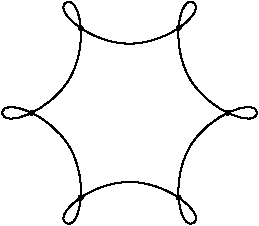
\includegraphics[height=1.1in]{main/Fig09-4A}}
\qquad
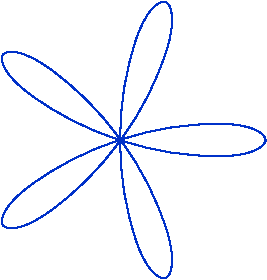
\includegraphics[height=1.2in]{main/five}
\caption{A general linear series of degree $g+2$ maps a nonhyperelliptic
curve of genus $g$
to a plane curve with $\protect\sbinom{g}{2}$ nodes 
but the image of a
hyperelliptic curve has
just one singular point, where $g$ smooth branches intersect with
distinct tangents.
}
\label{Fig9.4}
\end{figure}

\begin{proof}
%\begin{itemize}
% \item (Dimension) 
Since $D$ is general and $\deg D > h^{0}(K)$ we see
that $D$ is nonspecial, whence $h^0(D) = (g+2)-g+1 = 3$.
This yields the dimension claim.

%\item (no basepoints) 
If $|D|$ 
has
a basepoint $p\in C$, then $3=h^0(D)
= h^0(D-p) = (g+1)-g+1+h^0(K_C-D+p)$,
so $K_C-D$ is effective of degree $2g-2-(g+1) =g-3$; thus the family of
such $D$ depends on only $g-3+1$ parameters,
and $\mu(D)$ would lie in a proper subvariety of $\Pic_{g+2}(C)$,
contradicting generality.

Next we show that
there are only finitely many pairs $p,
q \in C$ such that $\phi_D(p) = \phi_D(q)$; that is, $\phi_D$
is birational onto its image. 
Indeed, $\phi_D(p) = \phi_D(q)$
 means that $h^0(D-p-q) = 2$. By the Riemann--Roch
 theorem, $D-p-q = K-E$ for some effective divisor $E$ of degree $g-2$;
 thus $\sO_C(D)$ is in the image of the map
$$
\nu : C_2 \times C_{g-2} \to \Pic_{g+2}(C)
$$
sending $(p+q, E)$ to $K_C - E + p + q$.
But
$\nu$ is
the composition of two surjective maps, $C_2 \times C_{g-2} \to C_g$
and $C_g\to Pic_g \to Pic_{g+2}$ by duality. Since the source and
target of $\nu$ have the same dimension, the general fiber of $\nu$ is
finite. 

We turn to the types of singularities. First we eliminate tacnodes.
To say that a pair of points $p, q \in C$ map to
a point of $C_0$ such that the
two branches have a common tangent means two things: that $h^0(D-p-q)
\geq 2$; and that $h^0(D-2p-2q) \geq 1$. If this is the case, set $E =
D - 2p - 2q$.  The condition $h^0(D-2p-2q) \geq 1$ is equivalent to
$E$ being an effective divisor. Considering the canonical map $\phi_K:
C\to \PP^{g-1}$
the 
geometric Riemann--Roch theorem,
\index{Riemann--Roch theorem!geometric}%
$$r(E) = \deg E -1-\dim\overlow{\phi_K(E)},$$ 
implies that $\overlow {\phi_K(E)}$ has
dimension $g-3$. The 
further
condition $h^0(D-p-q) \geq 2$ says that
$\dim\overlow{\phi_K(E+p+q)} = g-2$,
so the secant line $\overlw20{pq}$ meets the $(g-3)$-plane
$\overlow{\phi_K(E)}$. Now, not every secant line to $C$ can meet
a given linear subspace $\Lambda \subset \PP^{g-1}$ of dimension
$g-3$\emdash otherwise, the projection $\pi_\Lambda : C \to \PP^1$ would
be constant\emdash so we see that $\mu(D)$ would have to lie on the image
of a proper subvariety of $C_{g-2} \times C_2$ under the map $(E, p+q)
\mapsto \sO(E+2p+2q)$ from $C_{g-2} \times C_2$ to $\Pic_{g+2}(C)$.
Since the dimension of this subvariety is $<g$ we see that if $C'$ has
a point at which two branches are tangent, then $\sO_C(D)$ lies in a
proper subvariety of $\Pic_{g+2}(C)$. Since
the Abel--Jacobi map $C_{g+2} \to Pic_{g+2}(C)$ is surjective,
 $D$ would not be general.

\smallbreak
Now let's suppose that $C$ is nonhyperelliptic.
To prove 
claim (1) of the theorem,
we
have to show  
that the image $C_0 = \phi_D(C)$ 
has only nodes as singularities,
rather than cusps or triple points.
That there are exactly
$\tbinom{g}{2}$ nodes then follows from the 
adjunction formula.
\index{adjunction formula}%

\begin{itemize}
\item []\hskip-\leftmargini (no cusps)\, 
To say that a point $p \in C$ maps to a cusp of $C_0$
(that is, the differential $d\phi_D$ is zero at $p$) amounts to saying
that $h^0(D-2p) \geq 2$; that is, $D-2p$ is a $g^1_g$. But by the
Riemann--Roch theorem, $W^1_g = K_C - W_{g-2}$; so to say $\phi_D$
has a cusp means that
$$
\mu(D) \in 2W_1 + K_C - W_{g-2},
$$
and since the locus on the right has dimension at most $g-1$, a general
point of $J(C)$ will not lie in it. Note that this subsumes the fact
that $|D|$ has no basepoints.

\item []\hskip-\leftmargini (no triple points)\,
To say that $C_0$ has a triple point means
that for some divisor $E = p+q+r$ of degree 3, $h^0(D-E) \geq 1$; thus
we must have
$$
\mu(D) \in W_3^{} + W^1_{g-1}.
$$
To argue that this is not the case, we need to know that $\dim W^1_{g-1}
\leq g-4$; 
streamlined
if $C$ is nonhyperelliptic.
\end{itemize}

\noindent This concludes the proof in the nonhyperelliptic case. Now
suppose that $C$ is hyperelliptic, and let $|E|$ be the  $g^1_2$ on
$C$. 
Since $D$ is a
divisor of degree $g+2$, the divisor $D - E$ will
have degree $g$, and so be effective; thus we can write
$D \sim E + p_1 + \dots + p_g$
for some 
$g$ points $p_i$, which must be distinct since $D$ was assumed general.

The fact that
$$
h^0(D - p_1 - \dots - p_g) = h^0(E) = 2 = h^0(D) - 1
$$
implies that $\phi_D$ maps all the points $p_i$ to the same point. The
image curve $C_0$ thus has a point with at least $g$ branches. Since
these branches cannot share a tangent line,
they are smooth and their tangents are distinct; that is, the point is
an ordinary multiple point. By the adjunction
\index{adjunction formula}%
formula $p_a(C) = \tbinom{g+1}{2}$ and since $C$ has genus $g$ the
singularity must have $\delta$ invariant
$\tbinom{g+1}{2} -g = \tbinom{g}{2}$. Such a singularity cannot have
multiplicity $>g$, and is thus a $g$-fold point. Since the
$\delta$-invariant of such a point is at least $\tbinom{g}{2}$ by
the discussion following Theorem~\ref{divisor classes on blowup}
(see also
Proposition~\ref{effect of blowup on genus}), the $g$-fold point is ordinary and there can be no other
singularities.
\end{proof}

\section{Exercises}

\begin{exercise}
Let $C\subset \PP^r$ be a smooth curve 
over an algebraically closed field of arbitrary characteristic. 
We can
re-embed $C$ by a
Veronese map,
that is, consider $\widetilde C = \nu_m(C)$ where
$\nu_m :
\PP^r \to \PP^N$ is the $m$-th Veronese map. Prove:

\begin{proposition}[%
compare
~Proposition~\ref{nodal projection}]
\label{positive characteristic nodes}
If $m$ is high enough then
the projection of~$@\widetilde C$ from a general $\PP^{N-3}$
is a birational map onto a nodal
plane curve.
\unif
\end{proposition}

Hint: Show that the items of~
Theorem
\ref{needed for nodes}  are true in this
situation.
\end{exercise}


\begin{npt}
\begin{exercise}[\cite{Rathmann}]
\label{strange curves} Let $k$ be an
\index{Rathmann, J\"{u}rgen}%
algebraically closed field of characteristic $p>0$, and let $q=p^e$
for some $e\geq 1$. Let $C\subset \PP^r$
be the closure of the image $C_0$ of the morphism
$$
\AA^1 \ni t \mapsto (t, t^q, t^{q^2}, \dots , t^{q^{r}}) \in \AA^r
$$
where $\AA^r\subset \PP^r$ is the open set $x_0=1$.
\begin{enumerate}
\item Show that $C$ is a complete intersection, defined by the equations
$$
x_0^{q-1}x_2 - x_1^q, x_0^{q-1}x_3 - x_2^q,\dots,
x_0^{q-1}x_r - x_{r-1}^q.
$$
\item Show that $C$ is singular unless $q = r = 2$.
\item Show every secant line to $C_0$ contains $q$ points of $C_0$;
more generally, if
$a_1, \dots, a_r$ are linearly independent points of $C_0$, show that
the linear span of
$a_1, \dots, a_r$ contains $q^{(r-1)}$ points of $C_0$.  Compare this
with the configuration of
points in affine $r$-space over a field of $q$ elements.
\end{enumerate}
\end{exercise}
\end{npt}

\begin{exercise}
Here is another approach to the $g+2$ theorem in the hyperelliptic case:
\index{g@$g+2$ theorem}%
Let $C$ be a 
hyperelliptic
\index{hyperelliptic}%
curve of genus $g$ and $D$ a general divisor
of degree $g+1$ on $C$; let $|E|$ be the $g^1_2$ on $C$.
Consider the map $\phi : C \to \PP^1 \times \PP^1$ given as the product
of the maps $\phi_D : C \to \PP^1$ and $\phi_E : C \to \PP^1$ given by
the pencils $|D|$ and $|E|$.
\begin{enumerate}
\item Show that $\phi$ embeds the curve $C$ as a curve of bidegree
$(g+1,2)$ on $\PP^1 \times \PP^1` `$.
\item Now embed $\PP^1 \times \PP^1$ into $\PP^3$ as a quadric surface
$Q$; pick a general point $p \in C \subset Q$ and project $C$ from the
point $p$. Show that the image curve $C_0$ is a plane curve of degree
$g+2$ with one ordinary $g$-fold point.
\end{enumerate}

Hint: For the first part, show that $h^0(D - K_C) = 0$, and conclude
that the map $\phi_D \times \phi_E$ is birational onto its image; 
using
the genus formula, conclude the image curve is smooth. For the
second, observe that if $L$ is a line through $p$ meeting $C$ more than
once elsewhere, the line $L$ must be contained in $Q$.
\end{exercise}

\begin{exercise}\label{extremal m-ics}
Establish the analog of Proposition~\ref{rnc on most quadrics}
for hypersurfaces of any degree $m$, that is to say no irreducible,
nondegenerate curve in $\PP^d$ lies on more hypersurfaces of degree $m$
than the 
rational normal curve.
\index{rational normal curve}%
To do this, let $C\subset \PP^d$ be any irreducible nondegenerate
curve. Let $\Gamma$ be a general hyperplane section
of $C$, and use the exact sequences
$$
0 \to \cI_{C/\PP^d}(l-1) \to \cI_{C/\PP^d}(l) \to
\cI_{\Gamma/\PP^{d-1}}(l) \to 0.
$$
with $2 \leq l \leq m$ to show that
$$
h^0(\cI_{C/\PP^d}(m)) \leq  \mbinom{d+m}{m} - (md+1)
$$
with equality only~if $C$ is a rational normal curve.
\end{exercise}

\begin{exercise}\label{linear bound is sharp}
Let $D \subset \PP^r$ be a rational normal curve. If $\Gamma \subset D$
is any collection of $d$ points on $D$ (or for that matter any subscheme
of $D$ of degree $d$) then the 
Hilbert function
\index{Hilbert function}%
of $\Gamma$ is
$$
h_\Gamma(m) = \min\{d, mr+1\}
.
$$

Hint: If $d > mr$, then the hypersurfaces of degree $m$ containing
$\Gamma$ are exactly the hypersurfaces of degree $m$ containing $D$,
and we know how many there are. If $d \leq mr$, then the hypersurfaces
of degree $m$ containing $\Gamma$ cut out on $D$ the linear series
$|\cO_D(m)(-\Gamma))| = |\cO_{\PP^1}(mr-d)|$ and again we know the
dimension.
\end{exercise}

\begin{exercise}
Let $C$ be a reduced irreducible curve with general hyperplane section
$\Gamma$,
and write
$d-1 = M(r-1) +\epsilon$ with $\epsilon<r-1$ as in Castelnuovo's theorem.
Prove that
\begin{enumerate}
\item if $\epsilon > 0$, then $\cO_C(M)$ is nonspecial, but $\cO_C(M-1)$
is special; and
\item if $\epsilon = 0$, then $\cO_C(M-1)$ is nonspecial, but $\cO_C(M-2)$
\index{epsilon@$\epsilon$}%
is special.
\end{enumerate}

Hint: Show that if $h^{0}(\sO_{C}(m+1))-h^{0}(\sO_{C}(m)) \leq \deg C$,
and that if equality holds for
all $m\geq m_{0}$, then $\sO_{C}(m) $ is nonspecial for all $m\geq m_{0}$.
\end{exercise}

\begin{exercise}\label{castelnuovo unique}
If $C \subset \PP^r$ is a 
Castelnuovo curve
\index{Castelnuovo curve}%
of degree $d \geq 2r$,
show that $|D| = |\cO_C(1)|$ is the unique $g^r_d$ on $C$.

Hint: If $|D'|$ were another $g^r_d$ on $C$, show that $h^0(mD + D')
> h^0((m+1)D)$.
\end{exercise}


\begin{exercise}\label{rarity of Castelnuovo}
We have seen that complete intersections $C = Q \cap S \subset \PP^3$ of a
quadric surface $Q$ and a surface $S$ of degree $k$ achieve Castelnuovo's
bound $g = \pi(2k, 3)$ on the genus of curves of degree $2k$ in $\PP^3`
`$. In fact, we will see in Chapter~\ref{ScrollsChapter} that any curve
$C \subset \PP^3$ of degree $2k$ and genus $g = \pi(2k, 3) = (k-1)^2$
is of this form.
\begin{enumerate}
\item Find the dimension of the subvariety $\Gamma \subset M_g$ consisting
of Castelnuovo curves.
\item Find the dimension of the subvariety $H \subset M_g$ of
hyperelliptic curves, and compare this to the result of the first part.
\end{enumerate}

Hint: For 
(1), 
we can calculate the dimension of the Hilbert
scheme $\cH^\circ$ of 
Castelnuovo curves
\index{Castelnuovo curves}%
by calculating the dimension
of the incidence correspondence of pairs $(Q, C)$ with $Q$ a quadric
surface in $\PP^3$ and $C \subset Q$ a curve of type $(k,k)$; then invoke
Exercise~\ref{castelnuovo unique} to say the fibers of $\cH^\circ \to
M_g$ are isomorphic to 
\index{PGL@$\PGL_4$}%
\index{PGL@$\PGL_2$}%
$\PGL_4$.
For 
(2), 
we already know the
dimension of the locus of hyperelliptic curves is $2g-1$ ($2g+2$-tuples
of points in $\PP^1$ mod $\PGL_2$); the point is just that Castelnuovo
curves are rarer than hyperelliptic ones.
\end{exercise}





\input footer.tex

%header and footer for separate chapter files

\ifx\whole\undefined
\documentclass[12pt, leqno]{book}
\usepackage{graphicx}
\usepackage{eps-to-pdf}
\input style-for-curves.sty
%\input sl-macros.sty
\usepackage{hyperref}
\usepackage{showkeys} %This shows the labels.
\usepackage{msribib}
\usepackage{pdfpages}
\usepackage{draftwatermark}
\SetWatermarkText{DRAFT:\ \today}
\SetWatermarkScale{2}
\SetWatermarkColor[gray]{0.9}

%\usepackage{SLAG,msribib,local}
%\usepackage{amsmath,amscd,amsthm,amssymb,amsxtra,latexsym,epsfig,epic,graphics}
%\usepackage[matrix,arrow,curve]{xy}
%\usepackage{graphicx}
%\usepackage{diagrams}
%
%%\usepackage{amsrefs}
%%%%%%%%%%%%%%%%%%%%%%%%%%%%%%%%%%%%%%%%%%
%%\textwidth16cm
%%\textheight20cm
%%\topmargin-2cm
%\oddsidemargin.8cm
%\evensidemargin1cm
%
%%%%%%Definitions
%\input preamble.tex
%\input style-for-curves.sty
%\def\TU{{\bf U}}
%\def\AA{{\mathbb A}}
%\def\BB{{\mathbb B}}
%\def\CC{{\mathbb C}}
%\def\QQ{{\mathbb Q}}
%\def\RR{{\mathbb R}}
%\def\facet{{\bf facet}}
%\def\image{{\rm image}}
%\def\cE{{\cal E}}
%\def\cF{{\cal F}}
%\def\cG{{\cal G}}
%\def\cH{{\cal H}}
%\def\cHom{{{\cal H}om}}
%\def\h{{\rm h}}
% \def\bs{{Boij-S\"oderberg{} }}
%
%\makeatletter
%\def\Ddots{\mathinner{\mkern1mu\raise\p@
%\vbox{\kern7\p@\hbox{.}}\mkern2mu
%\raise4\p@\hbox{.}\mkern2mu\raise7\p@\hbox{.}\mkern1mu}}
%\makeatother

%%
%\pagestyle{myheadings}

%\input style-for-curves.tex
%\documentclass{cambridge7A}
%\usepackage{hatcher_revised} 
%\usepackage{3264}
   
\errorcontextlines=1000
%\usepackage{makeidx}
\let\see\relax
\usepackage{makeidx}
\makeindex
% \index{word} in the doc; \index{variety!algebraic} gives variety, algebraic
% PUT a % after each \index{***}

\overfullrule=5pt
\catcode`\@\active
\def@{\mskip1.5mu} %produce a small space in math with an @

\title{A Chapter from ``The Practice of Algebraic Curves"}
\author{\copyright David Eisenbud and Joe Harris}
%%\includeonly{%
%0-intro,01-ChowRingDogma,02-FirstExamples,03-Grassmannians,04-GeneralGrassmannians
%,05-VectorBundlesAndChernClasses,06-LinesOnHypersurfaces,07-SingularElementsOfLinearSeries,
%08-ParameterSpaces,
%bib
%}

\date{\today}
%%\date{}
%\title{Curves}
%%{\normalsize ***Preliminary Version***}} 
%\author{David Eisenbud and Joe Harris }
%
%\begin{document}

\begin{document}
\maketitle

\pagenumbering{roman}
\setcounter{page}{5}
%\begin{5}
%\end{5}
\pagenumbering{arabic}
\tableofcontents
\fi



\chapter{Monodromy of hyperplane sections}\label{uniform position}

\section{Uniform position and monodromy} \label{uniformSection}
We now return to the situation where the ground field $k$ is algebraically
closed of characteristic 0.

The central result of this chapter is the  
\emph{uniform position lemma}, 
\index{uniform position lemma}%
which deals with the monodromy group 
of the points of a general
hyperplane section of a curve $C \subset \PP^r` `$. To define the
monodromy group  and prove the  uniform position lemma, we will use the
classical topology. An equivalent algebraic definition is described in
Cheerful Fact~\ref{Galois equals monodromy} below, but the strong form
of uniform position can fail in positive characteristic,
as shown by the examples in Exercise~\ref{strange curves}.

We may describe the 
\blue{monodromy group}
\index{monodromy group|(}%
informally as follows: Suppose that
$C \subset \PP^r$ is an irreducible curve of degree $d$ over $\CC$,
and $H_0 \subset \PP^r$ a hyperplane transverse to $C$; say $C \cap
H_0 = \{p_1,\dots,p_d\}$. As we vary $H_0$ continuously along a real
arc $\{H_t\}$, staying within the open subset $U \subset (\PP^r)^*$
of hyperplanes transverse to $C$, we can ``follow'' each of the points
$p_i(t)$ of intersection of $C$ with the hyperplane $H_t$.

Now imagine that the hyperplanes $H_t$ come back to the original $H_0$
at time $t=1$; that is, we have a continuous family $\{H_t\}_{0 \leq
t \leq 1} \subset U$ with $H_1 = H_0$. Each of the points $p_i$ then
traces out a continuous real arc
$\{p_i(t) \in C \cap H_t\}_{0 \leq t \leq 1}$. Since $H_1 = H_0$, the
end point $p_i(1)$ is one of the original points $p_j \in C \cap H_0$. In
this way, we get a permutation of the set $C \cap H_0$; the group of all
permutations arrived at in this way is called the \emph{monodromy group}
\index{monodromy group|defi}%
of the points $C \cap H_0$.

We will now give a precise definition of the monodromy group in a more
general setting, and prove that the monodromy group of the points of a
general hyperplane section of an irreducible curve
 is the full symmetric group; this is the uniform position lemma. The
 rest of the chapter 
has
a series of applications.

\subsection*{The monodromy group of a generically finite morphism}

Let $f : Y \to X$ be a 
\blue{dominant map between varieties of the same dimension}
\index{dominant map!between varieties of same dimension}
over $\CC$, and suppose that $X$ is irreducible. There is then
a Zariski open subset $U \subset X$ such that $U$ and
its preimage $V = f^{-1}(U)$ are smooth, and the restriction of $f$
to $V$ is a covering space in the classical topology. Let $d$ be the
\index{sheets, number of}%
number of sheets. This is the degree of the extension $K(Y)/K(X)$.

\blue{Homotopy theory}
\index{homotopy theory}%
associates a monodromy group to any finite
topological covering map $f : V \to U$, defined as follows: Choose a
basepoint $p_0 \in U$, and suppose $\Gamma \colonequals  f^{-1}(p_0)  =
\{q_1,\dots,q_d\}$. If $\gamma$ is any loop in $U$ with basepoint $p_0$,
for any $i = 1, \dots, d$ there is a unique lifting of $\gamma$ to an
arc $\tilde \gamma_i$ in $V$ with initial point $\tilde \gamma_i(0)
= q_i$ and end point $\tilde \gamma_i(1) = q_j$ for some $j \in
\{1,2,\dots,d\}$. Since we could traverse the loop in the opposite
direction, the index $j$ determines $i$, and the map $i\mapsto j$ is a
permutation of $\{1,2,\dots,d\}$.
Since the set $\Gamma$ is discreet, the permutation depends only on the
class of $\gamma$ in $\pi_1(U,p_0)$, so we have defined a homomorphism
to the 
\blue{symmetric group:}
\index{symmetric group}%
$$
\pi_1(U,p_0)  \to \mathrm{ Perm}\,\Gamma \cong S_d.
$$
The image of this map,
 denoted in this chapter by $M$,
is called the \emph{monodromy group} of the
\index{permutation group|see symmetric group, $S_n$}%
map $f$. It depends on the labeling of the points of $\Gamma$, but a
change in labeling
only changes the group by conjugation with the corresponding permutation,
so the monodromy group is well defined up to
conjugation in $S_{d}$.
\vspace*{3pt}

\begin{fact}\label{Galois equals monodromy}
In our setting  the monodromy group is independent of the choice of open
set $U$: if $U' \subset U$ is a Zariski open subset, the complement of
$U\setminus U'$ has
real codimension $\geq 2$ so the map $\pi_1(U', p_0) \to \pi_1(U,p_0)$
is surjective. Thus the image of $\pi_1(U', p_0)$ in $S_d$ is the same.

The theory of finite coverings of algebraic varieties is not only
analogous to 
\index{Galois theory,}
it \emph{\bfseries{is}} Galois theory: In the situation
described above, if $Y$ is irreducible, then the pullback map $f^*$
expresses the function field $K(Y)$ as a finite algebraic extension of
$K(X)$. The monodromy group of $f$  is the Galois group of the Galois
\index{Galois normalization}%
normalization of $K(Y)$ over $K(X)$ (see \cite{Harris1979}). Indeed,
in early treatments of Galois theory, such as 
Camille Jordan's
famous \emph{Trait\'e
\index{Jordan, Camille}%
des substitutions} \citeyear{MR1188877}, 
function fields played as large a role as number fields.
\index{function field}%
\index{number field}%
\end{fact}

Since we assumed that $X$ is irreducible, the space $U$ is (path)
connected, and it follows that the monodromy group is transitive if and
\index{monodromy group!transitive}%
only~if the space $V$ is (path) connected. But $V$ is a smooth
variety, so this is the case if and only~if $V$ is irreducible. For
example, the monodromy in the family
of 
\blue{smooth quadric surfaces in $\PP^3$}
interchanges the two 
\blue{rulings:}
\index{ruling!interchange of --s}%
\index{quadric surfaces!in $\PP^3$}%

\begin{example}\label{monodromy of rulings}
Consider the family
$$
X \colonequals  \big\{@(p,Q) \mid p\in Q\hbox{ a point on a smooth quadric
surface in $\PP^3$}@\big\}
$$
of pointed smooth quadric surfaces in $\PP^3$ and the double covering by
$$
V\colonequals  \big\{@((p,Q), L)\mid (p,Q)\in X,\ L \hbox{ a line with $p
\in L\subset Q$}@\big\}.
$$
The variety $V$ is irreducible: if we project $V$ to the (irreducible)
variety of lines in $\PP^3` `$,
the fiber consists of a point on the line and quadric containing the
line\emdash that is, the product
of $\PP^1$ and the (dual of the) projective space
on the space of quadratic forms in the ideal of the line. Thus the
monodromy of the family
is transitive, and exchanges the two lines through the point.
\end{example}

\subsection*{Uniform position}


We will next compute the monodromy group of the  universal hyperplane
section of a curve, constructed as follows:
Let $C \subset \PP^r$ be an irreducible, nondegenerate curve of degree
$d$, and let $X = (\PP^r)^*$ be the space of hyperplanes in $\PP^r``$. 
We define the \emph{universal hyperplane section} of $C$ to be the
\index{universal hyperplane section|defi}%
projection  $f: Y\to (\PP^r)^*$ of the incidence variety
$$
Y = \{ (H, p) \in (\PP^r)^* \times C \mid p \in H \}.
$$
The fibers of $f$ are the hyperplane
sections of $C$, so $f$ is a finite surjective map. If we let $U\subset
(\PP^r)^*$ be the open subset of hyperplanes
meeting $C$ transversely, then the restriction of $f$ to the preimage $V$
of $U$ is a covering space
whose fibers each consist of $d$ distinct points. The preimage in $Y$
of a point $p\in C$ is the set of hyperplanes containing
$p$, a copy of $\PP^{r-1}$, and thus $Y$ is irreducible. Thus the
monodromy group of $f$ is transitive. But much more is true:

\begin{theorem}[uniform position lemma]
\label{uniform position lemma}
The 
monodromy group of the universal hyperplane section of an irreducible
curve $C \subset \PP^r$ is the full symmetric group~$S_d$.
\index{symmetric group}%
\end{theorem}

We postpone the proof to develop some necessary tools.

Theorem~\ref{uniform position lemma} fails over fields of finite
characteristic, though there is no known counterexample for smooth
curves; see Exercise~\ref{strange curves} for singular examples, and
\cite{Rathmann} and \cite{Kadets} for what is known.

Theorem~\ref{uniform position lemma} implies that two subsets of the
same cardinality in the general hyperplane section of $C$
are indistinguishable from the point of view of any discrete invariant
that is semicontinuous in the Zariski topology. To make this precise,
we introduce a definition:

\begin{definition}
Let $\phi : Y \to X$ be a finite morphism. By the 
\emph{restricted fiber power} 
\index{restricted fiber power|defi}%
$\tilde Y^n`/X$ we will mean the complement of all diagonals in
the ordinary fiber power; that is,
$$
\tilde Y^n`/X \colonequals  \bigl\{@ (x, y_1,\dots, y_n) \in X \times Y^n \mid
\phi(y_i) = x \text{ and } y_i \neq y_j \; \forall i \neq j @\bigr\}
$$
\end{definition}

In down-to-earth terms, a point of $\tilde Y^n`/X$ is a set of $n$
distinct points in a fiber of $\phi$ together with
the choice of a total order on these points.

\begin{lemma}\label{transitivity lemma}
Let $f : Y \to X$ be a generically finite cover of degree $d$, with
monodromy group $M \subset S_d$.
$M$ is $n$-transitive if and only~if the restricted fiber power $\tilde
Y^n`/X$ is irreducible.
\end{lemma}

\begin{proof}
If we restrict ourselves to open subsets $U \subset X$ and $V = f^{-1}(U)
\subset Y$ such that $U$ and $V$ are smooth and the restriction $f|_V :
V \to U$ is a covering in the classical topology, then the restricted
fiber powers are unions of connected components of the usual fiber
powers $Y^n`/X$. The condition that the monodromy is $n$-transitive is
equivalent to the condition that the restricted fiber power $\tilde Y^n`/X$
is connected; since the fiber powers are all smooth, this is equivalent
to $\tilde Y^n`/X$ being irreducible.
\end{proof}



\section{Flexes and bitangents are isolated}\label{isolated flexes
and bitangents}

There are  further general position results that we need for the proof
of the uniform position lemma.  We have separated
them from the results on linear general position because these require
characteristic 0; they are really local analytic
statements.

\subsection*{Not every tangent line is tangent at a flex}

%\label{isolated tangents and bitangents}

Recall that a smooth point $p$ on a curve $C \subset \PP^r$ is called
a \emph{flex point} if the tangent line to $C$ at  $p$ has contact of
\index{flex point}%
order 3 or more with $C$ at $p$.

\begin{lemma}\label{finite inflections}
If $r>1$ and $C \subset \PP^r$ is a smooth, irreducible and nondegenerate
curve, then not every point of $C$ is a flex point.
\unif
\end{lemma}

The proof applies to any linear series on a curve.
\unif

\begin{proof}
We begin by lifting the inclusion $C \hookrightarrow \PP^r$ to an arc
$v (t)$ in $\CC^{r+1}$, so that the tangent line at the point $t=0$
in projective space
is represented by the span of $v(0)$ and $v'(0) \in \CC^{r+1}$. To say
that $v(t)$ is a flex point is to say that the  vectors $v(t), v'(t)$
and $v''(t)$ are linearly dependent. If this holds for all $t$ then
$$
v(t) \wedge  v'(t) \wedge v''(t) \; \equiv \; 0.
$$

When we take the derivative of the wedge product $v(t) \wedge v'(t)
\wedge v''(t)$ by applying the product rule we see that the first two
terms are zero because they contain a repeated factor; it follows that
$$
v(t) \wedge  v'(t) \wedge v'''(t) \equiv 0,
$$
so that $v'''(t)$ lies in the span of $v(t)$ and $v'(t)$ as well. Indeed,
as we continue to take derivatives, we see in each case that all but one
term is zero, and we deduce that $v^{(l)}(p)$ lies in the span of $v(t)$
and $v'(t)$ for all $l$. This being characteristic 0, it follows that $C$
lies in a line, contrary to our hypothesis.
\end{proof}


\subsection*{Not every tangent is bitangent}

 This statement seems even more obvious than Lemma~\ref{finite
 inflections} above, but, like that lemma, it is false in
 characteristic $p$\emdash see Exercise~\ref{kaji}.


 \begin{lemma}\label{tangent not bitangent}
 Let $C \subset \PP^r$ be a smooth, irreducible, nondegenerate curve,
 with $r > 1$. If $p \in C$ is a general point, then the tangent line
 $\TT_p(C) \subset \PP^r$ is not tangent to $C$ at any other point.
\unif
 \end{lemma}

 \begin{proof} Again the result is local, this time with a pair of germs
 $D\ruto {\ v} ` `\PP^r$ and $D\ruto {\,w} ` `\PP^r` `$. If every
 tangent line to the two curves is a bitangent, we will show that they
 are both contained in a line.

  Let $C_1, C_2$ be the images of $v,w$ respectively, and let $\tilde v,
  \tilde w$ be lifts to $\CC^{r+1}$.
 Let
 $$
 \Sigma \colonequals  \bigl\{@ (p,q) \in D \times D \mid p\neq q \text{ and
 }\TT_{v(p)}(C_1) = \TT_{w(q)}(C_2)@ \bigr\}
 $$
 be the variety parametrizing bitangents to the two germs.



 The statement that the tangent lines to $C$ at the points $v(t)$
 and $w(t)$ are equal then says that the vectors $\tilde v(t), \tilde
 v'(t),\tilde w(t)$ and $\tilde w'(t)$ all lie in a 2-dimen\-sional subspace
 $\Lambda \subset \CC^{r+1}$; in particular,
 $$
 \tilde v(t) \wedge \tilde v'(t) \wedge \tilde w(t) \equiv 0 \quad
 \text{and likewise} \quad \tilde v(t) \wedge \tilde w(t) \wedge \tilde
 w'(t) \equiv 0
.
 $$

We proceed now exactly as in the proof of Lemma~\ref{finite inflections}:
taking derivatives, we see that all derivatives of $\tilde v(t)$
and $\tilde w$ at $t=0$ lie in $\Lambda$
and hence $C_1$ and $C_2$ are both contained in the line in $\PP^r$
corresponding to $\Lambda$.
 \end{proof}

In characteristic zero, \cite[Theorem 3.1]{kaji-tangentialDegeneracy}
shows that a general tangent line to a smooth projective curve $C$ can
intersect $C$ in a point other than $p$, except of course in case $r=2$,
although this is possible in characteristic $p>0$.

\section{Proof of the uniform position 
lemma
}

Let $C \subset \PP^r$ be an irreducible, nondegenerate curve of degree $d$
and 
let
$$f : Y \subset (\PP^r)^* \times C \to  X = (\PP^r)^*$$ 
be
its universal
hyperplane section; let $U \subset (\PP^r)^*$ be the open subset of
hyperplanes transverse to $C$ and $V = f^{-1}(U)$; let $M \subset S_d$
be the monodromy group of $V$ over $U$.
To show that  $M$ is the full symmetric group, it suffices to show that
$M$ contains all transpositions, and for this it is enough to show that
\index{doubly transitive}%
$M$ is doubly transitive and contains one transposition.

To prove that $M$ is doubly transitive, we can give a concrete description
\vadjust{\allowbreak}%
of the restricted fiber power $\tilde V^2`/U$: let
\index{restricted fiber power}%
$$
\Sigma \colonequals  \bigl\{@ (H, p, q) \in (\PP^r)^* \times C \times C
\mid p, q \in H \text{ and } p \neq q @\bigr\}.
$$
Projection on the second and third factors expresses $\Sigma$ as a
$\PP^{r-2}$-bundle over the complement $C \times C \setminus \Delta$
of the diagonal in $C \times C$. Thus $\Sigma$ is irreducible, and it
follows that the restricted fiber square $\tilde V^2`/U$, which is a
Zariski open subset of $\Sigma$, is as well. Note that this part of the
argument does not rely on any assumption about the characteristic.

Next we give a criterion for a monodromy group to contain a transposition:

\begin{lemma}\label{transposition lemma}
Let $f : Y \to X$ be a generically finite cover of degree $d$ over an
\index{transposition}%
irreducible variety $X$, with  monodromy group $M \subset S_d$.
If,  for some smooth point $p \in X$ the fiber $f^{-1}(p)\subset V$
consists of $d-2$ reduced points $p_1,\dots, p_{d-2}$ and one point $q$
of multiplicity \2, where $q$ is also a smooth point of $Y$, then $M$
contains a transposition.
\end{lemma}

\begin{figure}
\centerline {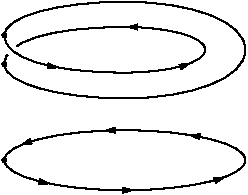
\includegraphics[height=1.4in]{main/Fig10-1}}
\vskip-5pt
\caption{Monodromy action around the ramification point of a double cover.}
\label{$d=2$ monodromy}
\end{figure}

See Figure~\ref{$d=2$ monodromy} for the case $d=2$.

\begin{proof} 
The hypothesis implies that $Y$ is smooth
locally near the fiber over $p$. Let $U \subset X$ be a Zariski open
subset of the smooth locus in $X$, as in the definition of the monodromy
group, so that  $V \colonequals  f^{-1}(U)$ is also smooth and the
restriction $f|_V : V \to U$ expresses $V$ as a finite $d$-sheeted
covering space of $U$, with $U,V$ smooth and $p\in X$.

Let $B_i\subset Y$ be disjoint small connected closed neighborhoods of
the points
in $f^{-1}(p)$. Because $f|_V$  is finite, the image $A \colonequals
\bigcap f(B_i)$  is a locally
closed subset of the same dimension as $X$ and thus $A$
 contains a neighborhood
of $p$ in the classical topology.

Let $p' \in A \cap U$. Two of the $d$ points of $f^{-1}(p')$  lie in the
component  of $B$ containing $q$; call these $q'$ and $q''$. Since $B
\cap V$ is the complement of a proper subvariety in $B$ it is connected,
and we can draw a real arc $\gamma : [0,1] \to B \cap V$ joining $q'$
to $q''$; by construction, the permutation of $f^{-1}(p')$ associated
to the loop $f \circ \gamma$  exchanges $q'$ and $q''$ and 
fixes
each
of the remaining $d-2$ points of $f^{-1}(p')$.
\end{proof}

\begin{proof}[Completion \kern1.5pt of \kern1.5pt the \kern1.5pt proof \kern1.5pt of \kern1.5pt 
Lemma~\ref{uniform position lemma}]%the \kern1.5pt uniform \kern1.5pt position \kern1.5pt lemma]
%\redden{What is left to show is}
%\marginpar{to allow line break}%
%Given Lemma~\ref{transposition lemma}, it remains to show
We  must show
that 
a reduced irreducible curve $C$ of degree $d$
 (in characteristic 0)
 has a hyperplane section consisting of $d-2$ smooth points and one
 double point; that is, a hyperplane simply tangent to the curve at one
 point and transverse everywhere else. By the results of
 Section~\ref{isolated flexes and bitangents} there is a tangent line $L$
 to $C$ at a smooth point that is not flex tangent, and is not tangent
 to $C$ at any other point. A general hyperplane $H$ containing $L$
 meets $C$ doubly in the point of
 tangency. At any other point $p$ of $L\cap C$, if any, the intersection
 $C\cap H$ is transverse
 unless $H$ contains the tangent line at $p$. Containing such a line is
 a  proper codimension 1 condition on
 the hyperplanes containing $L$, and since there can only be finitely
 many such points, a
 general  $H$ will be transverse at all such $p$. On the other hand,
 at points not on $L$
 the intersection $H\cap C$ is transverse by Bertini's theorem. This
 completes the proof.
\end{proof}

\subsection*{Uniform position for higher-dimensional varieties}

There is
a generalization of Theorem~\ref{uniform position lemma}
for irreducible varieties $X \subset \PP^r$ of any dimension $k$. To set
this up, let $\GG(r-k,r)$ be the 
\blue{Grassmannian}
\index{Grassmannian}%
parametrizing $(r-k)$-planes
$\Lambda \subset \PP^r` `$. We introduce the \emph{universal $(r-k)$-plane
section of} $X$:
$$
Y = \{ (\Lambda, p) \in \GG(r-k,r) \times X \mid p \in \Lambda \}.
$$
Via
projection on the first factor, $Y$ 
is expressed as a generically finite
cover of $\GG(r{@-@}k,r)$, and we can ask for its monodromy. The answer is
the same as for curves:


\begin{theorem}\label{higher dim uniform position lemma}
The monodromy group of the universal $(r-k)$-plane section of an
\index{monodromy group}%
\index{universal plane section}%
of the universal $(r-k)$-plane section of an
irreducible $k$-dimensional variety $X \subset \PP^r$ is the full
\index{symmetric group}%
\blue{symmetric group}
$S_d$.
\end{theorem}

\begin{proof}
This follows from Theorem~\ref{uniform position lemma}.
To see this,
fix a general $(r-k+1)$-plane $\Gamma \subset \PP^r$; since a
general hyperplane section of an irreducible variety $X \subset \PP^r$
of dimension $k \geq 2$ is again irreducible, we see that $C \colonequals
\Gamma \cap X$ is an irreducible curve. The restriction of the universal
$(r-k)$-plane section of $X$ to the sub-Grassmannian $\GG(r{@-@}k, \Gamma)
\cong (\PP^r)^*$ of $(r{@-@}k)$-planes contained in $\Gamma$ is just the
universal hyperplane section of the curve $C$, which we know has monodromy
$S_d$; since the monodromy group of a cover can only get smaller under
restriction to a subvariety of the target, the result follows.
\end{proof}

We will see an application of this result in 
Proposition~\ref{plane curve nodes}.

\section{Applications of uniform position}
\subsection*{Irreducibility of fiber powers}

If we apply the uniform position lemma to the universal hyperplane
section of a curve $C \subset \PP^r$ we get an irreducibility result:

\begin{corollary}\label{hyperplane section monodromy} If $C\subset \PP^r$
is a smooth curve of degree $d$, then
for $k\leq d$, the restricted fibered powers $\tilde Y^k`/X$  of the
universal hyperplane section
of $C$ are irreducible.
\end{corollary}

\subsection*{Numerical uniform position}

The property of uniform position, as exposed above, is really a property
of a family --- the irreducibility of the restricted
fiber powers --- and not of a given set of points. There is a useful
weaker property that
can be applied to a given set of points:

\begin{definition}
 A set of points $\Gamma\subset \PP^n$ is in \emph{numerical uniform
 position} if
 any two subsets of $\Gamma$ with the same cardinality impose the same
 number of conditions on forms of every degree $d$; that is, any two subsets
 of the same cardinality have the same Hilbert function.
%
\begin{figure}
\leavevmode
\vbox{\offinterlineskip
\hbox{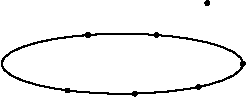
\includegraphics[scale=1.3,viewport=-10 37 118 39,clip]{main/Fig10-2}}%
\hbox{\includegraphics[scale=1.3,viewport=0 0 118 33,clip]{main/Fig10-2a}}}
\caption{
Seven
points in the plane,
of which six lie
on a conic. The seven are in linearly general 
position
but not 
in numerical
uniform position.}
\label{numerical uniform is stronger}
\end{figure}
%

This is strictly stronger than linearly general position, which 
involves only forms of degree $d=1$. The difference is illustrated
in Figure~\ref{numerical uniform is stronger}.
\end{definition}

\begin{corollary}[numerical uniform position lemma]\label{numerical
uniform position lemma}
The general hyperplane section of an irreducible curve
\index{numerical uniform position lemma}
$C\subset \PP^r$ is in numerical uniform position.
\unif
\end{corollary}

\begin{proof} Let $U = (\PP^r)^* \setminus C^*$ be the open subset
of hyperplanes transverse to $C$, and let $Y\to U$ be the universal
hyperplane section.
Corollary~\ref{hyperplane section monodromy} says that the restricted
fiber powers $\tilde V^n`/U$ are irreducible.

Now, for each $m$ the number of conditions that $\Gamma$ imposes on
forms of degree $m$ is lower semicontinuous, so it achieves its maximum
on a Zariski open subset of $\tilde V^n`/U$. Since $\tilde V^n`/U$ is
irreducible, the complement $Z$ of this open set has dimension strictly
less than $\dim \tilde V^n`/U = \dim U$. Thus a general hyperplane $H
\in (\PP^r)^*$  lies outside the image of $Z$, meaning that the number
of conditions imposed by all the $k$-element subsets $\Gamma \subset C
\cap H$ have this maximal value.
\end{proof}

This result may be seen as an important strengthening of
Theorem~\ref{basic linear independence}, since if $C$ is a reduced,
irreducible nondegenerate curve in $\PP^n$ then a general subset
of $n$ points of $C$ is linearly independent and spans a hyperplane;
Corollary~\ref{numerical uniform position lemma} says that this 
holds
for every subset of $n$ points of every general hyperplane section,
which reproves Theorem~\ref{basic linear independence}, though only in
characteristic~0.

\subsection*{Sums of linear series}

Another consequence of the uniform position lemma is a result about sums
\index{linear series!sums of}
of linear series.
Recall that if $D$ is a divisor on a curve $C$ we write $r(D) = \dim |D|
= h^0(\cO_C(D))-1$.

\begin{corollary}\label{Clifford equality plus}
If $D,E$ are effective divisors on a curve $C$ then
$$
r(D+E) \geq r(D)+r(E).
$$
If the genus of $C$ is $>0$ and $|D+E|$ is 
\blue{birationally very ample,}
\index{birationally very ample}%
\index{very ample!birationally}%
then the inequality is strict.
\end{corollary}

On $\PP^1` `$, by contrast, any effective divisor $D$ has $r(D) = \deg
D$, so the inequality above is
always an equality for $C = \PP^1` `$.

\begin{proof}
 The inequality follows in general because the sums of divisors in $|D|$
 and divisors in $|E|$ already move in
 a family of dimension $r(D)+r(E)$; the key point is the strict inequality
 in case $D+E$ is birationally very ample.

If $D+E$ is birationally very ample and $r(D+E) = r(D)+r(E)$ then
restricting to an open set
we may identify $C$ with its image under the complete linear series
$|D+E|$, and we see that a general hyperplane section $H\cap C$ contains
a divisor equivalent to $D$.

Let $Y$ be the $\deg D +\deg E$ restricted fiber power of the universal
hyperplane.
A point $y\in Y$ is a hyperplane section plus an ordering of its points.
Let $\phi: Y \to \Pic_d(C)$ be the 
\blue{Abel--Jacobi map}
\index{Abel--Jacobi map}%
 taking $y$
 to the class of the divisor that is the sum of first $d$ points in this
 order. The preimage  $Y'$ of the point of $\Pic_d(C)$ corresponding to
 the class of $D$ is a closed subset, and
since every divisor in the class of a hyperplane section contains
a divisor
linearly equivalent to  $D$, the subvariety $Y'$ dominates $(\PP^{n})^*$,
and thus
has the same dimension as~$Y$. Consequently $Y'=Y$, and the sum of the
first $d$ points
in any ordering of the general hyperplane section\emdash that is, the
sum of any $d$
of the points\emdash is equivalent to $D$.

Thus if $p\in D$ and $q\notin D$, then $D-p+q \equiv D$, whence $q\equiv
p$. Thus
$r(p)\geq 1$, so $C\cong \PP^1$.
\end{proof}

\subsection*{Nodes of plane curves}

\def\VD#1{V_{\mskip-5mu d,#1}} % compensate for huge gap in V_{d}

In Section~\ref{severi variety}, we introduced the \emph{Severi variety}
\index{Severi variety}%
$\VD{g}$; this is the locally closed subset of the projective space
$\PP^N$ of all plane curves of degree $d$ parametrizing irreducible
\marginpar{dropped $\delta:=$ to allow line break; it was anyway redefined again each time, except right after the next display, and in that case I expanded it (red expression below).}
plane curves of degree $d$ having 
$\tbinom{d-1}{2} - \nobreak g$ 
nodes and no other singularities. We proved there that $\VD{g}$ was
smooth, and by Cheerful Fact~\ref{severi irreducible} it is irreducible
for all $d$ and $g$.

To compute the monodromy we introduce the incidence correspondence
$$
\Phi \colonequals \big\{@(C, p) \in \VD{g} \times \PP^2 \mid p \in C_{\sing}
@\big\}.
$$
This is a
covering space of $\VD{g}$
with $\tbinom{d-1}{2} - \nobreak g$ sheets, 
and we compute its
monodromy. We start with the extremal case $g = 0$:

\begin{proposition}
The monodromy group of $\Phi$ over $\VD{0}$ is the full symmetric group
\label{plane curve nodes}
$S_\delta$, with $\delta = \tbinom{d-1}{2}$.
\end{proposition}

\begin{proof}
Every 
\blue{nodal curve}
\index{nodal curve}%
$C \subset \PP^2$ is the projection of a
\blue{rational normal curve}
\index{rational normal curve}%
$\tilde C \subset \PP^d$ from a $(d-3)$-plane
$\Lambda \subset \PP^d` `$. Moreover, if $\Lambda$ is general,  the nodes
of the projection correspond to the points of intersection of $\Lambda$
with the  
\blue{secant variety}
\index{secant variety}%
$X \subset \PP^d$ of the rational normal curve
$\tilde C$. Applying Theorem~\ref{higher dim uniform position lemma},
the result follows.
\end{proof}

This result has an immediate consequence, which played a major role in the
proof of Cheerful Fact~\ref{severi irreducible}: given the description in
Section~\ref{severi variety} of $\VD{g}$ in a neighborhood of a point
in $\VD{0}$, it follows that there is a unique irreducible component
of $\VD{g}$ containing $\VD{0}$ in its closure. Thus, to prove the
irreducibility of $\VD{g}$, it is sufficient to show that every component
of $\VD{g}$ contains $\VD{0}$ in its closure.

Going in the other direction, note also that if we assume Cheerful
Fact~\ref{severi irreducible}, then we can deduce the analogous result
for all $g$:


\begin{proposition}
The monodromy group of $\Phi$ over $\VD{g}$ is the full symmetric group
$S_\delta$, with $\delta = \tbinom{d-1}{2} - g$.
\end{proposition}



\section{Exercises}

As a consequence of Theorem~\ref{higher dim uniform position lemma},
we can deduce the 
\blue{Bertini irreducibility theorem:}
\index{Bertini irreducibility theorem}%

\begin{exercise}
Let $X \subset \PP^r$ be an irreducible variety of dimension $k \geq
2$. Show that a general hyperplane section of $X$ is irreducible.

Hint: Say $k=2$. If the general hyperplane section of $X$ were reducible,
there would be distinguished subsets of the intersection of $X$ with
a general $(r-2)$-plane $\Lambda$ (the intersections of $\Lambda$ with
the components of $H \cap X$, for $H$ a general hyperplane containing
$\Lambda$); but we know the monodromy on $X \cap \Lambda$ is the full
symmetric group.
\end{exercise}

\begin{exercise}
In Example~\ref{monodromy of rulings}, we gave a global argument to say
that in the family of smooth quadric surfaces in $\PP^3$ the monodromy
exchanges the two rulings of a quadric by lines. Prove this with a local
calculation, analyzing the family
$$
Q_t \colonequals  V(X^2+Y^2+Z^2 + tW^2)
$$
in a neighborhood of $t=0$.

Hint: Choose a basepoint of the pencil, say $p = [1, i, 0, 0]$. The
lines of the two rulings of $Q_t$ passing through $p$ are
$Y-iX = Z-\pm i@\sqrt{t}@W = 0$, which are exchanged under the monodromy
as $t$ goes around 0.
\end{exercise}

\begin{exercise}[tangential degeneracy {{\cite[Example 4.1]{kaji-tangentialDegeneracy}}}]
\label{kaji}
Show that the linear series 
in Exercise~\ref{1,d-1 on quadric}
\index{tangential degeneracy}%
defines an isomorphism with a smooth curve $C$ of type $(1, d-1)$ on a
nonsingular quadric in $\PP^2_k$ no matter what field $k$ is chosen. Now
suppose that  $k$ has characteristic $p>0$ and $d-1 = p^\ell n$ with
$\ell\ge 2$
and $n$ relatively prime to $p$.
Show that the tangent lines to $C$ are the rulings of the quadric in the
family that meet $C$ with multiplicity $d-1$, and that the intersection of
each tangent line meets $C$ in $n$ distinct points, each with multiplicity
$p^\ell$. Thus Lemma~\ref{tangent not bitangent}
fails in 
\blue{positive characteristic.} 
\index{positive characteristic}% 
\end{exercise}

\begin{exercise}
Let $C \subset \PP^r$ be a union of irreducible curves $C_i$ of degrees
$d_i$. Prove that the monodromy group of the points of a general
hyperplane section of $C$ is the product $\prod S_{d_i}$.

Hint: We need to know that the dual hypersurfaces $C_i^* \subset
(\PP^r)^*$ are all distinct; given this, we can exhibit loops that induce
a given permutation of the points of $H \cap C_i$ while fixing the points
of $H \cap C_j$ for $j \neq i$. To see that the dual hypersurfaces $C_i^*
\subset (\PP^r)^*$ are all distinct, invoke the duality theorem $(C_i^*)^*
= C_i$ (see for example \cite{3264}).
\end{exercise}

\begin{exercise}
Let $d$ and $e$ be positive integers, $\PP^M$ the space of plane curves
of degree $d$ and $\PP^N$ the space of plane curves of degree $e$, and
$$
\Phi \colonequals  \big\{@ (D, E, p) \in \PP^M \times \PP^N \times \PP^2 \mid
p \in D \cap E@\big \}.
$$
Prove that the monodromy group of the projection $\pi : \Phi \to \PP^M
\times \PP^N$ is the symmetric group $S_{de}$ on $de$ letters
\begin{enumerate}
\item by applying Theorem~\ref{uniform position lemma}; and
\item from scratch, using the method used in the proof of
Theorem~\ref{uniform position lemma}.
\end{enumerate}

Hint: for the first part, we can fix the curve $E$ and prove the
a priori stronger statement that the monodromy on the points of
$D \cap E$ as $D$ varies is the symmetric group; this follows from
Theorem~\ref{uniform position lemma} applied to the Veronese embedding
$\nu_d(E)$. Alternatively, we can exhibit a transposition by finding a
pair $(D,E)$ such that $D \cap E$ consists of $de-2$ simple points and
one double point, and prove double transitivity with the usual incidence
correspondence argument.
\end{exercise}

\begin{exercise}
If $E \subset \PP^2$ is a smooth plane cubic curve, then a point $p \in E$
is called a 
\blue{\it flex} %
\index{flex}%
if $\cO_E(3p) \cong \cO_E(1)$ (see Chapter~\ref{InflectionsChapter} for a generalization). By Corollary~\ref{torsion
points} in case $g=1$, there are nine of them. Now let $\PP^9$ be the
space of 
\blue{plane cubics, }
\index{plane cubics}%
and let
$$
\Phi \colonequals  \big\{@(E, p) \in \PP^9 \times \PP^2 \mid p \text{ is a
flex of } E@ \big \}.
$$
Show that the monodromy group of $\Phi \to \PP^9$ is a proper subgroup
of $S_9$.

Hint: the line joining any two flexes of a plane cubic $E$ contains
a third.
\end{exercise}

\begin{exercise}
Let $C$ be a smooth projective curve. Show that if $\pi : C \to \PP^1$
is a simply branched cover of degree $n$, then the monodromy of the map
$\pi$ is the full symmetric group $S_n$.

Hint: Show that a transitive subgroup of $S_n$ generated by 
\blue{transpositions}
\index{transposition}%
is all of $S_n$.
\index{monodromy group|)}%
\end{exercise}

\input footer.tex
%header and footer for separate chapter files

\ifx\whole\undefined
\documentclass[12pt, leqno]{book}
\usepackage{graphicx}
\usepackage{eps-to-pdf}
\input style-for-curves.sty
%\input sl-macros.sty
\usepackage{hyperref}
\usepackage{showkeys} %This shows the labels.
\usepackage{msribib}
\usepackage{pdfpages}
\usepackage{draftwatermark}
\SetWatermarkText{DRAFT:\ \today}
\SetWatermarkScale{2}
\SetWatermarkColor[gray]{0.9}

%\usepackage{SLAG,msribib,local}
%\usepackage{amsmath,amscd,amsthm,amssymb,amsxtra,latexsym,epsfig,epic,graphics}
%\usepackage[matrix,arrow,curve]{xy}
%\usepackage{graphicx}
%\usepackage{diagrams}
%
%%\usepackage{amsrefs}
%%%%%%%%%%%%%%%%%%%%%%%%%%%%%%%%%%%%%%%%%%
%%\textwidth16cm
%%\textheight20cm
%%\topmargin-2cm
%\oddsidemargin.8cm
%\evensidemargin1cm
%
%%%%%%Definitions
%\input preamble.tex
%\input style-for-curves.sty
%\def\TU{{\bf U}}
%\def\AA{{\mathbb A}}
%\def\BB{{\mathbb B}}
%\def\CC{{\mathbb C}}
%\def\QQ{{\mathbb Q}}
%\def\RR{{\mathbb R}}
%\def\facet{{\bf facet}}
%\def\image{{\rm image}}
%\def\cE{{\cal E}}
%\def\cF{{\cal F}}
%\def\cG{{\cal G}}
%\def\cH{{\cal H}}
%\def\cHom{{{\cal H}om}}
%\def\h{{\rm h}}
% \def\bs{{Boij-S\"oderberg{} }}
%
%\makeatletter
%\def\Ddots{\mathinner{\mkern1mu\raise\p@
%\vbox{\kern7\p@\hbox{.}}\mkern2mu
%\raise4\p@\hbox{.}\mkern2mu\raise7\p@\hbox{.}\mkern1mu}}
%\makeatother

%%
%\pagestyle{myheadings}

%\input style-for-curves.tex
%\documentclass{cambridge7A}
%\usepackage{hatcher_revised} 
%\usepackage{3264}
   
\errorcontextlines=1000
%\usepackage{makeidx}
\let\see\relax
\usepackage{makeidx}
\makeindex
% \index{word} in the doc; \index{variety!algebraic} gives variety, algebraic
% PUT a % after each \index{***}

\overfullrule=5pt
\catcode`\@\active
\def@{\mskip1.5mu} %produce a small space in math with an @

\title{A Chapter from ``The Practice of Algebraic Curves"}
\author{\copyright David Eisenbud and Joe Harris}
%%\includeonly{%
%0-intro,01-ChowRingDogma,02-FirstExamples,03-Grassmannians,04-GeneralGrassmannians
%,05-VectorBundlesAndChernClasses,06-LinesOnHypersurfaces,07-SingularElementsOfLinearSeries,
%08-ParameterSpaces,
%bib
%}

\date{\today}
%%\date{}
%\title{Curves}
%%{\normalsize ***Preliminary Version***}} 
%\author{David Eisenbud and Joe Harris }
%
%\begin{document}

\begin{document}
\maketitle

\pagenumbering{roman}
\setcounter{page}{5}
%\begin{5}
%\end{5}
\pagenumbering{arabic}
\tableofcontents
\fi


\chapter{Brill--Noether theory and applications to genus 6}\label{Brill--Noether}\label{BNChapter}

\section{What linear series exist?}

Let's start with a naive question: when does there exist a curve $C$ of genus $g$ and a $g^r_d$ on $C$\emdash equivalently, a line bundle $\cL$ of degree $d$ on $C$ with $h^0(\cL) \geq r+1$? The Riemann--Roch and Clifford theorems together provide a complete answer to this question:

\begin{theorem}\label{arbitrary linear series}
There exists a curve $C$ of genus $g$ and a line bundle $\cL$ of degree $d$ on $C$ with $h^0(\cL) \geq r+1$ if and only if
$$
r \leq
\begin{cases}
d-g, \quad \text{if } d \geq 2g-1; \text{ and} \\
d/2,  \quad \text{if } 0 \leq d \leq 2g-2.
\end{cases}
$$
\end{theorem}


For the\emdash perhaps more interesting\emdash question of when  there exists a curve of genus $g$ with a birationally very ample $g^r_d$, Castelnuovo's theorem gives a quadratic bound, roughly $d \geq \sqrt{g(2r-2)}$.

In both these situations, the curves that achieve the bounds are quite special. Perhaps the most interesting question of all is, for which $r,d$ do \emph{all} curves of genus $g$ have a $g^r_d$, and what is the
behavior of these series on a general curve? Brill--Noether theory provides some answers to both these questions.

\section{Brill--Noether theory}

The following result was stated by Brill and Noether in 1874, and finally proven in a series of works by
\cite{Kempf}, \cite{MR323792}, \cite{MR0357398}, \cite{Kleiman-special} culminating in a paper by
Griffiths and the second author~\cite{Griffiths-Harris-BN}.

\begin{theorem}[Basic Brill Noether]\label{basic BN}
If $r\geq 0$ and
 $$
 \rho(g,r,d) := g - (r+1)(g-d+r) \geq 0,
$$
then every smooth projective curve of genus $g$  possesses a $g^r_d$. Conversely, if $\rho < 0$ then a general curve $C$ of genus $g$ does not possess a $g^r_d$.
\end{theorem}

%\begin{theorem}[Basic Brill Noether]\label{basic BN}
%A general curve $C$ of genus $g$  possesses a linear series of degree $d$ and dimension $r>d-g$ if and only if
%$$
% \rho(g,r,d) := g - (r+1)(g-d+r) \geq 0.
%$$
%\end{theorem}

It is interesting to compare the values of $d,r$ that are possible on special and general curves; see Figure~\ref{Clifford-Castelnuovo-BrillNoether comparison}.

\begin{figure}
\inprogress     
\centerline {\includegraphics[height=3in]{"main/Fig11-1-Clifford-Castelnuovo-Brill-Noether"}}
\caption{For smooth curves of genus 100, 
these are bounds on $(d,r)$ for all linear series (Clifford), 
birationally very ample series (Castelnuovo), and all linear series
on general curves (Brill--Noether). }
\label{Clifford-Castelnuovo-BrillNoether comparison}
\end{figure}
%\fix{vert axis should be labeled $r$, horizontal labeled $d$. Color might
%be good to make the regions clearer.}

Gathering the inequalities, and putting them all in terms of lower bounds on $d$ given $g, r$,
we get \goodbreak
%$$
\begin{align*}
 d &\geq \min\{r+g, 2r\} \hbox{ by the Riemann--Roch and Clifford theorems}\\
 d &\geq \sqrt{(2r-2)g} \hbox{ by an approximation to the Castelnuovo theorem}\\
 d &\geq r+g-\frac{g}{r+1} \hbox{ for a general curve.}
\end{align*}
%$$

In the following sections, we'll explain the heuristic argument that led Brill and Noether to the statement of Theorem~\ref{basic BN} and discuss some refinements.   In Chapter~\ref{InflectionsChapter} we'll give a proof based on the study
of inflections and on families of Jacobians.% \fix{char 0?}.

The case $r=1$ is already interesting:

\begin{corollary}
If $C$ is any curve of genus $g$, then $C$ admits a map  to $\PP^1$ of degree $d$ for some $d \leq \lceil \frac{g+2}{2}\rceil$.
\end{corollary}

Thus any curve of genus 2 is hyperelliptic, any curve of genus 3 or 4 is either hyperelliptic or trigonal  (admits a 3-1 map to $\PP^1$), and so on. We have already verified this assertion in genus $g \leq 5$ by analyzing the geometry of the canonical map; for higher genera, though, this is not feasible.

Note also that this is exactly the converse to Corollary~\ref{branched cover BN} of Chapter~\ref{ModuliChapter}.


\subsection{A Brill--Noether inequality}\label{BN by divisors}

The proof of the Brill--Noether theorem starts with a dimension estimate that was first carried out by Brill and Noether in 1874 \cite{Brill-NoetherOriginal}. The estimate provides an inequality on the dimension
of the variety $W^r_d$, and the assertion of the theorem is that this is sharp for a general curve.

%From Kleiman-Laksov:  For r= 1, the matter is treated in section 4 of Riemann's " Theorie der Abel'schen Functionen" [11] (1857) and in lecture 31 of Hensel-Landsberg(1902) 1; the general case is treated in Brill--Noether [1](1874) and in lecture 57 and appendix G of Severi [13].(1921)

Let $C$ be a smooth projective curve of genus $g$, and $D = p_1 + \dots + p_d$ a divisor on $C$. Assume for simplicity that  the points $p_i$ are distinct; the same argument  can be carried out in general, but requires more complicated notation.

When does the divisor $D$ move in an $r$-dimensional linear series? By the Riemann--Roch theorem $h^0(D) \geq r+1$ if and only if the vector space $H^0(K-D)$ of 1-forms vanishing on $D$ has dimension at least $g-d+r$\emdash that is, if and only if the  evaluation map
$$
H^0(K) \to H^0(K|_D) = \bigoplus k_{p_i}
$$
has rank at most $d-r$. 

We can represent this map by a $g \times d$ matrix. Choose a basis $\omega_1,\dots,\omega_g$ for the space $H^0(K)$ of 1-forms on $C$; choose an analytic open neighborhood $U_j$ of each point $p_j \in D$ and choose a local coordinate $z_j$ in $U_j$ around each point $p_j$, and write
$$
\omega_i = f_{i,j}(z_j)dz_j
$$
in $U_j$. We  have $r(D) \geq r$ if and only if the  matrix-valued function
$$
A(z_1,\dots,z_d) = 
\begin{pmatrix}
f_{1,1}(z_1) & f_{2,1}(z_1) & \dots & f_{g,1}(z_1) \\
f_{1,2}(z_2) & f_{2,2}(z_2) & \dots & f_{g,2}(z_2) \\
\vdots & \vdots &  & \vdots \\
f_{1,d}(z_d) & f_{2,d}(z_d) & \dots & f_{g,d} (z_d)
\end{pmatrix}
$$
has rank $d-r$ or less at $(z_1,\dots,z_d) = (0,\dots,0)$.


In the space $M_{d,g}$ of $d \times g$ matrices, the subset of matrices of rank $d-r$ or less has codimension $r(g-d+r)$ (\cite[Exercise 10.9]{Eisenbud1995}. 
It follows 
that if  an effective divisor $D$ of degree $d$ with $h^0(D) \geq r+1$ exists, then in a neighborhood of the point $D \in C_d$ the locus $C^r_d$ of such divisors must have dimension at least $d - r(g-d+r)$, with equality if the map $A$ is dimensionally transverse to the locus in $M_{d,g}$ of matrices of rank at most $d-r$. Since a general fiber of the map $\mu : C^r_d \to W^r_d(C)$ has dimension $r$, it follows that 
$$
\dim W^r_d(C) \geq d - r(g-d+r) - r = g - (r+1)(g-d+r)
$$
and this is exactly the  Brill--Noether (in)equality. We will give a proof of the Brill--Noether theorem in Chapter~\ref{BrillNoetherproofChapter}.


\subsection{Refinements of the Brill--Noether theorem}

Theorem~\ref{basic BN} suggests a slew of questions, both about the geometry of the schemes $W^r_d(C)$ parametrizing linear series on a general curve $C$ (are they irreducible? what are their singular loci,\dots), and about the geometry of the linear systems themselves (do they give embeddings? what's the Hilbert function of the image? \dots). This is an active area of research. Here is some of what is currently known, starting with results about the geometry of $W^r_d(C)$:

\begin{theorem}\label{Wrd omnibus}
Let $C$ be a general curve of genus $g$. If we set $\rho = g - (r+1)(g-d+r)$, then for $d \leq g+r$,
\begin{enumerate}

\item $\dim(W^r_d(C)) = \rho$ (\cite{Griffiths-Harris-BN});\label{GH}

\item\label{sing wrd} the singular locus of $W^r_d(C)$ is exactly $W^{r+1}_d(C)$
(\cite{Gieseker-Petri}, \cite{Lazarsfeld-Petri};
\label{irr wrd} 

\item if $\rho > 0$ then $W^r_d(C)$ is irreducible (\cite{MR611386});

\item\label{rho=0} if $\rho = 0$ then $W^r_d(C)$ consists of a finite set of  points of cardinality
$$
\#W^r_d(C) = g! \prod_{\alpha=0}^r \frac{\alpha!}{(g-d+r+\alpha)!}
$$
and the monodromy of the generically finite covering of  $M_g$ by the universal family
$\cW^r_d$ of $W^r_d$s is transitive.
(\cite{zbMATH04014883}).

\item\label{Petri} if  $\sL$ is an invertible sheaf on $C$, then the multiplication map
$$
m : H^0(L) \otimes H^0(\omega_C\otimes L^{-1}) \rTo H^0(\omega_C)
$$
is injective, and the Zariski tangent space to the scheme $W^r_d(C)$ at the point $L$, as a subspace
of the tangent space $T_L\pic_d(C) = H^0(\omega_C)^*` `$, is the annihilator of the image of $m$
or, equivalently, the kernel of the dual of $m$ (\cite{Gieseker-Petri}).
\end{enumerate}
\end{theorem}

\begin{corollary}\label{2L nonspecial}
If $C$ is a general curve and $\sL$ is a general point of $W^r_d(C)$ with $r\geq 2$,
 then $\sL^m$ is nonspecial for all $m \geq 2$.
\end{corollary}

\begin{proof}
If $\sL^m$ were special\emdash that is, if $\omega_C\otimes \sL^{-m} = E$ were effective\emdash then we would have an inclusion $H^0(\sL) = H^0(\omega_C\otimes \sL^{-m+1}(-E)) \hookrightarrow H^0(\omega_C\otimes \sL^{-m+1})$. By Part~\ref{Petri} of Theorem~\ref{Wrd omnibus}, the map 
 $$
m : H^0(\sL^{m-1}) \otimes H^0(\omega_C\otimes \sL^{-m+1}) \rTo H^0(\omega_C)
$$
is injective, so the map
$$
H^0(\sL^{m-1}) \otimes H^0(\sL) \subset H^0(\sL^{m-1}) \otimes H^0(\omega_C\otimes \sL^{-m+1})
$$
obtained by restriction would likewise be injective.
However if $\sigma, \tau \in H^0(\sL)$ are two linearly independent sections, then $\sigma^{m-1} \otimes \tau - \sigma^{m-2}\tau \otimes \sigma$ lies in the kernel, contradicting the specialness of $\sL^m` `$.
\end{proof}

\begin{remark}

\begin{enumerate}
 \item As a special case of Part~\ref{rho=0} of the Theorem we see that the number of $g^{1}_{d}$s
 in the case $\rho=0$, that is, $g=2d-2$, is the Catalan number $C_{d-1}:= \frac{1}{d}\binom{2d}{d}$.

We have already seen this in the first two cases: in genus 2, it says the canonical series $|K|$ is the unique $g^1_2$ on a curve of genus 2, and in the case of genus 4 we have already seen  that there are exactly two $g^1_3$s on a general curve of genus 4. In genus 6, it says that a general curve of genus 6 has 5 $g^1_4$s; we'll describe these in Section~\ref{general genus 6} below.  

\item Part~\ref{Petri} and Part~\ref{GH} imply Part~\ref{sing wrd}. \cite[Section IV.4]{ACGH} shows that at a point $\sL  \in W^r_d(C) \setminus W^{r+1}_d(C)$, the tangent space to $W^r_d$ at the point $\sL $ is the annihilator
in $(H^0(\omega_C))^*$ of the image of $\mu$; given that $\mu$ is injective, we can compare dimensions and deduce that $W^r_d$ is smooth at $\sL $.

\item For any curve $C$, there exists a scheme $G^r_d(C)$ parametrizing linear series of degree $d$ and dimension $r$; that is, in set-theoretic terms,
$$
G^r_d(C) = \left\{ (\sL , V) \mid \sL  \in Pic_d(C), \text{ and } V \subset H^0(\sL ) \text{ with } \dim V = r+1 \right\}.
$$
$G^r_d(C)$ maps to $W^r_d(C)$; the map is an isomorphism over the open subset $W^r_d(C) \setminus W^{r+1}_d(C)$ and has positive-dimensional fibers over $W^{r+1}_d(C)$. It was conjectured
by Petri and proven in \cite{Gieseker-Petri} that for a general curve the scheme $G^r_d(C)$ is smooth for any $d$ and $r$.
\end{enumerate}
\end{remark}


Recall that  in theorems~\ref{g+1 theorem}, \ref{g+2 theorem}, \ref{g+3 theorem} we proved that
general invertible sheaves of degrees $g+1$, $g+2$ and $g+3$ on any curve
give the nicest possible maps to (respectively) $\PP^1, \PP^2$ and $\PP^3.$ These
linear series, being general of degree $\geq g$, are  nonspecial and have respectively
2, 3, or 4-dimensional spaces of sections. The following result shows that something
similar is true on a general curve for general linear series with 2,3, or 4-dimensional
spaces of sections, though they may have degrees much less than $g+1, g+2, g+3$:

\begin{theorem}\label{grd omnibus}(\cite[Proposition 5.4]{Eisenbud-Harris83}
Let $C$ be a general curve of genus $g$, and suppose that
$|D|$ is a general $g^r_d$ on $C$.

 \begin{enumerate}
\item If $r \geq 3$ then $D$ is very ample; that is, the map $\phi_D : C \to \PP^r$   embeds $C$ in $\PP^r` `$;
\item If $r=2$ the map $\phi_D : C \to \PP^2$ gives a birational embedding of $C$ as a nodal plane curve; and 
\item If $r=1$, the map $\phi_D : C \to \PP^1$ expresses $C$ as a simply branched cover of $\PP^1` `$.
\end{enumerate}
\end{theorem}

In case $\rho = 0$\emdash so that there are a finite number of $g^r_d$s on a general curve $C$\emdash these statements hold for \emph{all} the $g^r_d$s on $C$.

In the course of investigating embeddings of a curve $C\subset \PP^n$ we have again and again
asked about the ranks of the maps $H^0(\sO_{\PP^n}(d)) \to H^0(\sO_C(d))$. In the case of
a general curve, the following theorem of \cite{Larson} gives a comprehensive answer; in particular, it gives
 the Hilbert function of any general embedding:
 
\begin{theorem}[E. Larson](Maximal Rank theorem)\label{maximal rank}
If $C$ is a general curve of genus $g$ and $\sL  \in W^r_d(C)$ is a general point, then for each $m > 0$ the multiplication map
$$
\rho_m : \Sym^m H^0(\sL ) \to H^0(\sL ^m)
$$
has maximal rank; that is, it is injective if $\binom{m+r}{r} \leq h^0(\sL ^m)$ and surjective if $\binom{m+r}{r} \geq h^0(\sL ^m)$.
\end{theorem}


If $\sL\in W^r_d(C)$ is a general point, then Corollary~\ref{2L nonspecial} shows that 
$h^0(\sL ^m) = md-g+1$ for all $m \geq 2$
and this allows us to compute the Hilbert function of a general embedding as a curve
of degree $d$ as 
 $$
 h_C(m) = \min\left(\binom{m+r}{r},\ md-g+1\right).
 $$
 
A key step in Larson's proof is an interpolation theorem~\cite{MR3908670}, later extended in~\cite{MR4653767} to show:

\begin{theorem}[\cite{MR4653767}]\label{Larson-Vogt}
Let $d, g$ and $r$
be nonnegative integers with $\rho(d, g, r) \geq 0$. There is a general curve of degree $d$ and genus $g$ through $n$ general
points in $\PP^r$
if and only if
$$
(r-1)n \leq (r + 1)d-(r-3)(g-1)
$$
except in the four cases $(d, g, r) = (5, 2, 3)$,
$(6, 4, 3)$, $(7, 2, 5)$ and $(10, 6, 5)$.
 \end{theorem}
 
There is a possible extension of the maximal rank theorem. If $C \subset \PP^r$ is a general curve embedded by a general linear series, the maximal rank theorem tells us the dimension of the $m$th graded piece of the ideal of $C$, for any $m$: this is just the dimension of the kernel of $\rho_m$. But it doesn't tell us the degrees of generators of the homogeneous ideal of $C$. For example, if $m_0$ is the smallest $m$ for which $I(C)_m \neq 0$, or numerically the smallest $m$ such that $\binom{m+r}{r} > md-g+1$, we can ask: is the homogeneous ideal $I(C)$ generated by $I(C)_{m_0}$? This can't always be the case, since 
there are examples where the  smallest nonzero graded piece of $I(C)$ has dimension 1. But one might conjecture that $I(C)$ is always be generated by its graded pieces of degrees $m$ and $m+1$; this is an open problem.

To answer this\emdash given that we know the dimensions of $I(C)_m$ for every $m$\emdash we would need to know the ranks of the multiplication maps
$$
\sigma_m : I(C)_m \otimes H^0(\cO_{\PP^r}(1)) \to I(C)_{m+1}
$$
for each $m$. In particular, we may conjecture that \emph{the maps $\sigma$ have maximal rank}; if this were true we could deduce the degrees of a minimal set of generators for the homogeneous ideal $I(C)$.

Another recent strand of work on Brill--Noether theory was developed in the thesis
\cite{HLarson} and in \cite{arXiv:2008.10765}, providing  analogues of many of the parts of the classical Brill--Noether theorem
for general curves of given gonality in the cases $\rho\geq 0$.


There are many remaining questions! One is the question of \emph{secant planes}: a naive dimension count would suggest that an irreducible, nondegenerate curve $C \subset \PP^r$ should have an $s$-secant $t$-plane if and only if $s(r-t-1) \leq (t+1)(r-t)$
(for example a curve $C \subset \PP^3$ has 4-secant lines, but no 5-secant lines). Is this true for a general curve embedded in $\PP^r$ by a general linear series?

\begin{exercise}
We saw in Chapter~\ref{JacobianChapter} that if $C$ is any curve of genus $g$ and $D$ a general divisor of degree $g+3$ on $C$, then $\phi_D : C \hookrightarrow \PP^3$ is an embedding. Using the Brill--Noether theorem, show that if $C$ is general then the image curve in $\PP^3$ has no 5-secant lines.
\end{exercise}

\section{Linear series on curves of genus 6}\label{genus 6 section}\label{general genus 6}
%\fix{This will come after the plane curves: we get the 5-ic del Pezzo for free, given the "conditions of adjunction", and then
%the special cases will give us exercise in what the conditions of adjunction are.}

We have seen in our analysis of curves of genus up to 5 that curves of the same genus can look quite different from the point of view of the linear series they possess: the existence of $g^r_d$s,  the geometry of the schemes $W^r_d(C)$ parametrizing them, and the geometry of the associated maps to projective space, can look quite different on different curves.

The variety of possible behaviors has increased modestly with the genus. Genus 6 is a tipping point: we could still enumerate all the possible behaviors of the schemes $W^r_d(C)$\emdash as distinguished by the number of components, dimension and singularities of the various schemes $W^r_d(C)$, and the geometry of the associated maps\emdash but it's quite a long list, and we will actually study just a few cases. For genus 7 and higher a full analysis has probably never been carried out. 

In lower genus we tacitly verified the statements of the Brill--Noether theorem from our descriptions of the canonical models. In genus 6, by contrast, we cannot  deduce the Brill--Noether theorem from studying the geometry of the canonical curve\emdash though we can easily see that a canonical curve $C \subset \PP^5$ of genus 6 lies on a 6-dimensional vector space of quadrics, that doesn't tell us much about its geometry.

Instead we will appeal directly to the Brill--Noether theorems. Here is a summary of what we will use:

\begin{theorem}\label{BN consequences}
Every smooth curve $C$ of genus 6 has at least one $g^{2}_{6}$. If $C$ is general, then
$W^{2}_{6}(C)$ and $W^{1}_{4}(C)$ each consist of 5 reduced points, while $W^{2}_{5} = W^{1}_{3} = \emptyset$.  Less formally, C has precisely 5 $g^{2}_{6}$s and 5 $g^{1}_{4}$s, but no $g^{2}_{5}$s and no $g^{1}_{3}$s. The image of the map associated to each $g^{2}_{6}$ is a nodal plane curve and its nodes are in linearly general position, that is, no three are collinear.
\end{theorem}

All these assertions except for the linear general position of the nodes follow immediately from 
Theorem~\ref{basic BN} and
Theorem~\ref{Wrd omnibus}; we will deduce the linear general position of the nodes from the relationship of the different
linear series on a general curve that are given by these theorems.

%\subsection{Linear series on general curves of genus 6}\label{general genus 6}
\subsection{General curves of genus 6}
\emph{We suppose for the rest of this section that $C$ is a general smooth curve of genus 6.}

By Theorem~\ref{BN consequences} we can map $C$ birationally to a plane sextic $C_0$ with only nodes as singularities. Since a plane sextic has arithmetic genus $\binom{6-1}{2} = 10$, the curve $C_{0}$
must have exactly 4 nodes.

Once we have exhibited one birational map of $C$ to a plane sextic with 4 nodes, we can describe all five $g^2_6$s and all five $g^1_4$s in terms of this plane model. For example, composing a $g^1_6$ corresponding to $f: C\to \PP^1$ with the projections from the 4 nodes gives four $g^1_4$s. To see the 5th $g^{1}_{4}$ we introduce some terminology:

Suppose $f : X \to S$ is a regular map from any smooth curve $X$ to a surface $S$. If $\sL $ is a line bundle on $S$ and $V \subset H^0(\sL )$ a vector space of sections, we can associate to them a linear system on $X$ by taking the pullback linear system $f^*V \subset H^0(f^*\sL )$ on $X$ and subtracting the basepoints; this is called the \emph{linear series cut out on $X$ by $V$}. 

To see the $g^{1}_{4}$s on $C$ in this way,  suppose again that $C$ is a general curve of genus 6 as above and $f : C \to \PP^2$ is a birational map onto a sextic curve $C_0$ with four nodes; let $p \in C_0$ be one of the nodes and consider the linear system $(\cO_{\PP^2}(1),V)$ of lines in $\PP^2$ through $p$. The pullback $f^*\cO_{\PP^2}(1)$ of course has degree 6, but the pullback linear series $f^*V$ has two basepoints, at the points $q, r \in C$ lying over $p$. The linear series cut on $C$ by $V$ is thus a $g^1_4$. 

To produce the fifth $g^1_4$, consider the linear series cut on $C$ by conic plane curves passing through all four nodes of $C_0$. There is a pencil of such conics, and the pullback $f^*\cO_{\PP^2}(2)$ has degree 12.
If the nodes are linearly independent then the pullback series has eight basepoints; thus we arrive at another $g^1_4$ on $C$.  Not all the nodes can be contained in a line, since then, by B\'ezout's theorem, the line would be a component of $C_0$. Thus if the nodes are linearly dependent, then exactly 3 lie on a line
so the linear series cut by the conics containing the nodes coincides with the projection from the 4th node. 
This would represent a nonreduced point of the scheme $W^1_4(C)$, the subject of Exercise~\ref{nonreduced Wrd} below. Thus the nodes are independent.

For another example, consider the linear system cut on $C$ by cubics passing through all four nodes. This has degree $3\cdot 6 - 8 = 10$ and dimension 6. It follows that this is the complete canonical series on $C$. (In Chapter~\ref{PlaneCurvesChapter} we will see directly that this is the case.)

Given the degree six map $f : C \to C_0 \subset \PP^2$ corresponding to one $g^2_6$ we can use the fact that the five $g^2_6$s on $C$ are residual to the five $g^1_4$s in the canonical series to construct the other four $g^2_6$s: they are cut out on $C$ by the linear system of plane conics passing through three of the four nodes of $C_0$. Equivalently, their images are the curves obtained from $C_{0}$ by the quadratic transformation
of $\PP^{2}$ centered at 3 of the 4 nodes, which blows up these 3 nodes and blows down the three lines
 joining them.
 
 In previous chapters we have seen that in genus $\leq 5$ a general canonical curve is  a complete intersection, but this fails for a canonical curve $C$ of genus 6. There is a 21-dimensional vector space of
quadratic forms on $\PP^5` `$, and $h^0(\sO_C(2)) = 2(2g-2)-g+1 = 15$, so $C$ lies on at least 6 quadrics, and we will show that its ideal sheaf is generated by exactly 6 quadrics. Since $6>\codim C$, the canonical curve of genus 6 is not a complete intersection. However, such curves lie on a quintic del Pezzo surface, which may be described as follows.


%There is a further consequence of this description: the four nodes of $C_0$ are in linear general position; that is, no three are collinear. 
%By parts~(\ref{rho=0}) and~\ref{Petri} of Theorem~\ref{Wrd omnibus}, $C$ must have 5 distinct $g^1_4$s, and if three of the four nodes of $C_0$ were collinear, the $g^1_4$ cut on $C$ by lines through the fourth node would coincide with the $g^1_4$ cut on $C$ by conics through all four.  
%
 
\begin{figure}
\centerline {\includegraphics[height=2in]{"main/Fig11-2"}}
\caption{A $g^1_4$ as the projection from a node of a plane sextic.
\marginparhere{Silvio: both lines of the projection should meet the sextic 4 times; the dashed line could be tangent. In general, perhaps our convention for showing a map by projection should be to show more than two projection lines (and note that they are all on the same footing).}
}
\end{figure}

\begin{figure}
\centerline {\includegraphics[height=2in]{"main/Fig11-3"}}
\caption{A $g^1_4$ as a pencil of hyperbolas through the four nodes of a plane sextic.}
\end{figure}
 
 
\begin{figure}
\centerline {\includegraphics[height=2in]{"main/Fig11-4"}}
\caption{A sextic with 4 nodes and the fundamental triangle of the quadratic transformation giving
a different $g^{2}_{6}$. 
\marginparhere{Silvio: nice picture. Might be better to use color for
  the three lines of the distinguished triangle. Is the sextic
  mathematically correct? If not, it might be clearer if the lines of
  the triangle weren't so tight to the sextic\emdash they are a little
  hard to distinguish.}
}
\end{figure}


\subsection{Del Pezzo surfaces}\label{Del Pezzo sketch}

We  met the del Pezzo surface of degree 5 in Section~\ref{Genus 1 quintics in P4}. 
We briefly sketch, without proofs, a little of the 
 rich classical theory of del Pezzo surfaces in general. The basics are well treated in \cite[pp. 45--50]{Beauville}; for more, see the
beautiful book \cite{Manin}, which also goes into some of the arithmetic theory. We will use only the case of the del Pezzo surface of degree 4, which lies in $\PP^{5}$

By definition,
a \emph{del Pezzo} surface is a smooth surface embedded in $\PP^n$  by its complete anticanonical series $-K_S$. These exist only for $3\leq n\leq 9$. The best-known example is a smooth cubic surface in $\PP^3` `$. That it is a del Pezzo surface follows from the adjunction formula.

A del Pezzo surface in $\PP^n$ has degree $n$, and is isomorphic to the blow-up of $\PP^2$ at $9-n$ points of which no 3 lie on a line and no 6 lie on a conic, embedded by the linear series on $\PP^2$
consisting of the cubics passing through the $9-n$ points\emdash except when $n=8$, in which case the
linear series of curves of type $(2,2)$ on $\PP^1\times \PP^1$ provides another example.

Comparing the linear series  of cubic forms containing $p_1,\dots,p_4$ with the linear series  of sextic forms vanishing to order 2 at $p_1,\dots,p_4$, we see that a quintic del Pezzo surface $S \subset \PP^5$ lies on at least $5$ quadrics. In fact, its homogeneous ideal is generated by exactly 5 quadrics.

A quintic del Pezzo surface $S \subset \PP^5$ contains exactly 10 lines, which (in terms of the description of $S$ as the blow up of $\PP^2$ at four points $p_1,\dots,p_4 \in \PP^2$) are the 4 exceptional divisors and the 6 proper transforms of the lines joining the $p_i$ pairwise. 
It is the intersection of a $\PP^5$ with the Grassmannian $G(2,5) \subset \PP^9` `$, and correspondingly the five quadrics containing $S$ can be realized as the Pfaffians of a  $5\times 5$ skew-symmetric matrix of linear forms on $\PP^5` `$.

\begin{figure}
\centerline {\includegraphics[height=1.6in]{"main/Fig11-5"}}
\caption{Dual graph of the configuration of 10 lines on a quintic del Pezzo surface, the plane blown up
at 4 points showing 4 pairwise disjoint exceptional divisors.}
\label{dual graph of the configuration of 10 lines on a quintic del Pezzo surface}
\end{figure}

There is also a notion of a \emph{weak del Pezzo} surface; this is a smooth surface whose anticanonical bundle is nef but not necessarily ample. We get such a surface if we blow up $\PP^2$ at a configuration of points of which three are collinear; in this circumstance the anticanonical bundle on the blow-up $S$ has degree 0 on the proper transform of the line containing the three points, and this proper transform is correspondingly collapsed to a rational double point of the image $\phi_{-K}(S)$. In general, the description of del Pezzo surfaces as blow-ups of the plane extends to the case of weak del Pezzos.



\subsection{The canonical image of a general curve of genus 6}

Using the Brill--Noether theorem, we have seen that a general curve $C$ of genus 6 is the normalization of a plane sextic $C_0$ with four nodes, and that the canonical series on $C$ is cut out by cubics in the plane passing through the four nodes. Thus the canonical model lies on the surface $S \subset \PP^5$ that is the image of the plane under the (rational) map given by cubics through these four points, which we now recognize as a quintic del Pezzo surface.

\begin{theorem}
A general canonical curve $C$ of genus 6 is the intersection of a quintic del Pezzo surface and a quadric. 
\end{theorem}

\begin{proof}
We have seen that $C \subset \PP^5$ lies on a quintic del Pezzo surface $S \subset \PP^5` `$. The surface is cut out by 5 quadrics, and we know that $C$ lies on 6 independent quadrics,
so $C$ is contained in the complete intersection of $S$ with a quadric. Since this scheme has degree 10, which is the degree of $C$, they are equal.
\end{proof}

For corresponding theorems for general curves with $g=7,8,9$ see \cite{Mukai1}, \cite{Mukai2}, and \cite{Mukai3}.


\section{Other curves of genus 6}

From Theorem~\ref{BN consequences} we know that every curve $C$ of genus 6 has  a $g^{2}_{6}$. For a general curve the corresponding morphism $\phi_{D}$ maps $C$ birationally onto a plane sextic with 4 nodes and exactly 5 $g^{1}_{4}$s. 
In this  section we will analyze some of the other curves of genus 6, starting with the question  ``what could go wrong?"
with the birational map to $\PP^2` `$. 

Since we already have a complete picture in the hyperelliptic case, we'll assume that $C$ is nonhyperelliptic. Clifford's theorem then rules out
the existence of a $g^3_6$ so  the $g^2_6$ is a complete linear series  $|D|$ for some divisor $D$ of degree 6.

Further analysis can be divided as follows:
\begin{enumerate}
\item $C$ is not trigonal. Then either
\begin{enumerate}
 \item $|D|$ has a basepoint; the canonical image of $C$ lies on the Veronese surface.
\item $\phi_{D}$ maps $C$ two to one onto a cubic $E \subset \PP^2$ of genus 1; the canonical image is the complete intersection of a quadric and the cone over the elliptic quintic $E\subset \PP^{4}$.
\item $\phi_{D}$ is birational onto a plane sextic with no triple point.
 \end{enumerate}
 \item $C$ is trigonal. The canonical image lies on a 
rational normal scroll $S(a,4-a)$; see Chapter~\ref{ScrollsChapter}.
In this case $|D|$ is base-point free and $\phi_{D}$  either maps $C$ three to one onto a conic
 or birationally onto a sextic with a triple point. 
\end{enumerate}

In the rest of this section we will examine cases 1a and 1b. Case 2 can be further divided by the value of $a$.
Case 1c may be divided into many parts according to the various configurations
of double points of the plane sextic, which may be nodes, cusps, tacnodes or higher-order double points,  corresponding to various possible schemes $W^{1}_{4}$. 

The analysis of the other cases is lengthy, but largely accessible with the tools we've introduced.


\subsection{$|D|$ has a basepoint}\label{g26 has a basepoint}
Clifford's theorem shows that a nonhyperelliptic curve of genus 6 cannot have a $g^2_4$, so   
$|D|$ has exactly one basepoint, and when we subtract the basepoint we get a base-point-free $g^2_5$. 

If $C \to C_0 \subset \PP^r$ is the map given by a base-point free $g^r_d$, the degree $d$ of the linear series is the degree of the image curve $C_0$ times the degree of the map $C \to C_0$. Since 5 is prime, the associated map $\phi_D : C \to \PP^2$ is birational onto a quintic curve. Moreover, since plane quintic curves have arithmetic genus 6, the image $\phi_D(C)$ is smooth; thus $C$ is isomorphic to a smooth plane quintic.

This allows us to describe the other special linear series on $C$. By the adjunction formula, the canonical series $|K_C|$ is cut on $C$ by conics in the plane. 

The plane $\PP^2$ is embedded by the complete linear series of quadrics as the Veronese surface in $\PP^5` `$, and since the canonical series of $C$ is cut out by quadrics, the canonical model of $C$
lies on this surface, and the canonical ideal is generated by the 6-dimensional family of quadrics containing the Veronese surface\emdash the $2\times 2$ minors of the generic symmetric $3\times 3$ matrix
corresponding to the multiplication map 
$$
H^{0}(\sO_{\PP^{2}}(1)) \otimes H^{0}(\sO_{\PP^{2}}(1)) \to H^{0}(\sO_{\PP^{2}}(2))
$$
as explained in Proposition~\ref{some equations}-- together with a 3-dimensional family of cubics,  the image of the 3 dimensional family of forms of degree 6 that are multiples of the quintic form defining $C$ in $\PP^2` `$.

As we showed in Chapter~\ref{3b}, the $g^1_4$s on $C$ are exactly the projections from points of $C$, so $W^1_4(C)\cong C$, and there are no 
$g^{1}_{3}$s.


\subsection{$C$ is not trigonal and the image of \texorpdfstring{$\phi_{D}$}{phi(D)} is two to one onto a  plane curve of degree 3.}

The cubic curve $E$ is smooth since otherwise it would have geometric genus 0 and $C$ would be  hyperelliptic. Thus $C$ is a double cover of a smooth curve of genus 1; we say that $C$ is \emph{bielliptic}.

In this case the canonical divisor class $K_C$ is the pullback of an invertible sheaf $\cO_E(F)$ for some divisor class of degree 5 on $E$. But it is not the case that the canonical series $|K_C|$ is the pullback of the linear series $|\cO_E(F)|$: by the Riemann--Roch theorem, the latter has dimension 4, rather than 5. Indeed, if we recall that the target of the canonical map $\phi_K : C \to \PP^5$ is the projective space $\PP H^0(K_C)$, there is be a point $X \in \PP^5$ corresponding to the hyperplane $\pi^*H^0(F) \hookrightarrow H^0(K_C)$, and projection of the canonical curve from this point maps $C$ 2-to-1 onto the image $\phi_F(E) \subset \PP^4` `$. In other words, the canonical model of $C$ lies on a cone $S = \overline{X, E}$ over an elliptic normal quintic curve $E \subset \PP^4` `$. 

As we saw in Chapter~\ref{3b}, the quintic curve $\phi_F(E) \subset \PP^4$ lies on 5 quadrics, as does the cone $S \subset \PP^5$ over it. Thus there is a quadric $Q \subset \PP^5$ containing $C$ but not containing $S$. B\'ezout's theorem shows that in this case, the canonical model of a bielliptic curve of genus 6 is the intersection of the cone over an elliptic quintic curve with a quadric.

\section{Exercises}

\begin{exercise}
Let $C$ be a bielliptic curve of genus 6; that is, a double cover of a  smooth projective curve $E$ of genus 1. 
\begin{enumerate}
\item Show that $C$ cannot be hyperelliptic (going forward, we will identify $C$ with its canonical image in $\PP^5$).
\item Let $F$ an invertible sheaf of degree 5 on $E$ and $\phi_F(E) \subset \PP^4$ the corresponding elliptic normal quintic curve. Show that $\phi_F(E)$ lies on 5 quadrics, as does the cone $S \subset \PP^5$ over it
\item Deduce that there is a quadric $Q \subset \PP^5$ containing $C$ but not containing $S$. Now invoke B\'ezout's theorem to deduce that in this case, the canonical model of a bielliptic curve of genus 6 is the intersection of the cone over an elliptic quintic curve with a quadric.
\end{enumerate}

Hint: For the second part, we know that $\phi_F(E)$ lies on at least 5 quadrics by the usual restriction sequence; if it lay on 6 or more it would be a rational normal curve. (Alternatively, see Section~\ref{g=1 in P4}.)
\end{exercise}


\begin{exercise}
Use the preceding exercise to show that if $C$ is a bielliptic curve of genus 6, a 2-sheeted cover of an elliptic curve $E$, then every $g^1_4$ on $C$ is the pullback of a $g^1_2$ on $E$, and likewise  every $g^2_6$ on $C$ is the pullback of a $g^2_3$ on $E$. Deduce that in this case, $W^1_4(C)$ and $W^2_6(C)$ are each isomorphic to $E$.

Hint: Use the description of the canonical model of $C$ and the geometric Riemann--Roch theorem.
\end{exercise}


\begin{exercise}
Let $C$ be a trigonal curve of genus 6 with $g^1_3$ $|E|$, and $p \in C$ a general point. Show that the linear series $|K_C - E-p|$ is a $g^2_6$, and that the corresponding map $C \to \PP^2$ maps $C$ birationally onto a plane sextic curve with a triple point.
\end{exercise}


\begin{exercise}\label{plane models}
Let $C$ be the normalization of a plane sextic $C_0$ with four nodes, three of which are colinear. Show that by choosing a different $g^2_6$ on $C$, we can express it as the normalization of a plane sextic with two nodes and a tacnode.

Hint: Take the image of $C$ under the map associated to the $g^2_6$ cut out by conics through two of the three collinear nodes and the one remaining node.
\end{exercise}


\begin{exercise}
Show that if $C$ is the normalization of a plane sextic $C_0$ with only double points, then $W^1_4(C) \cong W^2_6(C)$ is zero-dimensional (so in particular this case does not overlap with any of the previous cases)
\end{exercise}


\begin{exercise}
Find an example of a curve $C$ of genus 6 such that $W^1_4(C)$ consists of one point of degree 5. Bonus points for showing that in this case the scheme $W^1_4(C) \cong \Spec \CC[\epsilon]/(\epsilon^5)$.
\end{exercise}

Hint: the curve in question is the normalization of a plane sextic curve with one double point, consisting of two smooth branches with contact of order 4 with each other and contact of order 3 with their common tangent line. The exercise asks you to both prove that such a curve exists, and that the $g^1_4$ cut out by lines through the double point is the unique $g^1_4$ on $C$. 

\begin{exercise}
Show that if $C$ is a smooth plane quintic, then the $g^2_6$s on $C$ all have a basepoint; that is, they are all of the form $|K_C| + p$ for $p \in C$. 

Furthermore, the canonical model of $C$ will lie on a quadratic Veronese surface $S$; and the six
quadrics containing the canonical curve $C$ are the six quadrics containing $S$ (in particular, the intersection of the quadrics containing $C$ will be $S$, so
the ideal of $C$ requires generators of degree $>2$.
\end{exercise} 

\begin{exercise}\label{nonreduced Wrd}
Show that if the nodes of the curve $C_0$ are in linear general position\emdash that is, no three collinear\emdash then indeed the map $\mu : H^0(D) \otimes H^0(K-D) \to H^0(K)$ is an isomorphism for each of the five $g^1_4$s on $C$.
\end{exercise}





\input footer.tex
%header and footer for separate chapter files

\ifx\whole\undefined
\documentclass[12pt, leqno]{book}
\usepackage{graphicx}
\usepackage{eps-to-pdf}
\input style-for-curves.sty
%\input sl-macros.sty
\usepackage{hyperref}
\usepackage{showkeys} %This shows the labels.
\usepackage{msribib}
\usepackage{pdfpages}
\usepackage{draftwatermark}
\SetWatermarkText{DRAFT:\ \today}
\SetWatermarkScale{2}
\SetWatermarkColor[gray]{0.9}

%\usepackage{SLAG,msribib,local}
%\usepackage{amsmath,amscd,amsthm,amssymb,amsxtra,latexsym,epsfig,epic,graphics}
%\usepackage[matrix,arrow,curve]{xy}
%\usepackage{graphicx}
%\usepackage{diagrams}
%
%%\usepackage{amsrefs}
%%%%%%%%%%%%%%%%%%%%%%%%%%%%%%%%%%%%%%%%%%
%%\textwidth16cm
%%\textheight20cm
%%\topmargin-2cm
%\oddsidemargin.8cm
%\evensidemargin1cm
%
%%%%%%Definitions
%\input preamble.tex
%\input style-for-curves.sty
%\def\TU{{\bf U}}
%\def\AA{{\mathbb A}}
%\def\BB{{\mathbb B}}
%\def\CC{{\mathbb C}}
%\def\QQ{{\mathbb Q}}
%\def\RR{{\mathbb R}}
%\def\facet{{\bf facet}}
%\def\image{{\rm image}}
%\def\cE{{\cal E}}
%\def\cF{{\cal F}}
%\def\cG{{\cal G}}
%\def\cH{{\cal H}}
%\def\cHom{{{\cal H}om}}
%\def\h{{\rm h}}
% \def\bs{{Boij-S\"oderberg{} }}
%
%\makeatletter
%\def\Ddots{\mathinner{\mkern1mu\raise\p@
%\vbox{\kern7\p@\hbox{.}}\mkern2mu
%\raise4\p@\hbox{.}\mkern2mu\raise7\p@\hbox{.}\mkern1mu}}
%\makeatother

%%
%\pagestyle{myheadings}

%\input style-for-curves.tex
%\documentclass{cambridge7A}
%\usepackage{hatcher_revised} 
%\usepackage{3264}
   
\errorcontextlines=1000
%\usepackage{makeidx}
\let\see\relax
\usepackage{makeidx}
\makeindex
% \index{word} in the doc; \index{variety!algebraic} gives variety, algebraic
% PUT a % after each \index{***}

\overfullrule=5pt
\catcode`\@\active
\def@{\mskip1.5mu} %produce a small space in math with an @

\title{A Chapter from ``The Practice of Algebraic Curves"}
\author{\copyright David Eisenbud and Joe Harris}
%%\includeonly{%
%0-intro,01-ChowRingDogma,02-FirstExamples,03-Grassmannians,04-GeneralGrassmannians
%,05-VectorBundlesAndChernClasses,06-LinesOnHypersurfaces,07-SingularElementsOfLinearSeries,
%08-ParameterSpaces,
%bib
%}

\date{\today}
%%\date{}
%\title{Curves}
%%{\normalsize ***Preliminary Version***}} 
%\author{David Eisenbud and Joe Harris }
%
%\begin{document}

\begin{document}
\maketitle

\pagenumbering{roman}
\setcounter{page}{5}
%\begin{5}
%\end{5}
\pagenumbering{arabic}
\tableofcontents
\fi


\chapter{Inflection points}\label{inflections chapter}
\label{InflectionsChapter}

Generalizing the ramification points of a map from a smooth curve $C$
\index{flex|see inflection point}%
to $\PP^1` `$, there are finitely many ``special'' points determined by
any linear series on any curve, the \emph{inflection points}.
\index{inflection point}%
We love this topic for its echoes of classical algebraic geometry and
it will provide the tools to give a proof of the Brill--Noether
theorem in the following chapter. In characteristic 0 every linear
series has finitely many inflection points, and the number of these,
properly counted, depends only on the genus of the curve and the
degree of the linear series.

\section{Inflection points,  Pl\"ucker formulas and Weierstrass points}

\subsection*{Definitions}
To characterize the inflection points of a linear series 
$\sD = (\sL, V)$ on a curve $C$, we will use the following result:

\begin{proposition}\label{vanishing sequence} Let $V$ be a
\index{vanishing sequence}%
  finite-dimensional vector space of 
global sections
\index{global section}%
of an 
invertible sheaf
\index{invertible sheaf}%
$\sL$ on a smooth curve $C$, and let $p \in C$
be a point. There exists a basis $\sigma_0, \dots, \sigma_r$ of $V$
consisting of sections vanishing to different orders at~$p$. Thus the set 
$$
\{ \ord_p(\sigma) \mid \sigma \neq 0 \in V \}
$$
 has cardinality $\dim V` `$.
\unif
\end{proposition}

\begin{proof} 
Let $\tau_0, \dots, \tau_r$ be any basis of $V` `$.  If  $\tau_i$ and
$\tau_j$ vanish to the same order at~$p$, then
some nonzero linear combination $\tau_i' \colonequals  a\tau_i+b\tau_j$
vanishes to strictly higher order. Since the coefficients $a$ and $b$
are both necessarily nonzero we may modify the basis, replacing $\tau_i$
with $\tau_i'$, strictly increasing the sum of the orders.
The order of vanishing of each $\sigma_i$ is bounded above by $\deg \sL$,
so the sum of the orders is bounded by $(r+1)\deg \sL$. Thus the process
must terminate, and when it does,
 the orders must be distinct.
\end{proof}

According to  Proposition~\ref{vanishing sequence}, if $\cD = (\cL, V)$
is any $g^r_d$ on $C$, we may write
$$
\{ \ord_p(\sigma) \mid \sigma \neq 0 \in V \} = \{a_0,\dots,a_r\} \;
\text{ with } \; 0\leq a_0 < a_1 < \dots < a_r.
$$
The sequence $a_i = a_i(\cD,p)$ is called the
\index{vanishing sequence|defi}%
\emph{vanishing sequence} of $\cD$ at $p$.  Since $a_i \geq i$,
the numbers
$\alpha_i = \alpha_i(\cD,p) \colonequals  a_i - i$ are often more
interesting,
and the sequence $0 \leq \alpha_0 \leq \alpha_1 \leq \dots \leq
\index{ramification sequence|defi}%
\alpha_r$ is called the \emph{ramification sequence} of $\cD$ at $p$.

We say that $p$ is an \emph{inflection point} of the linear series $\cD$
if $(\alpha_0,\dots,\alpha_r) \neq (0,\dots,0)$\emdash equivalently,
if $\alpha_r > 0$\emdash and we define the \emph{weight} of $p$ to be
\index{weight!of an inflection point}%
$$
w(\cD, p) = \sum_{i=0}^r \alpha_i(\cD, p)
$$
and the 
\emph{inflectionary divisor}
\index{inflectionary!see divisor, inflectionary}%
\index{divisor!inflectionary}%
 on $C$ to be 
$$
\sum_{p\in C}w(\cD, p)p.
$$

If $\cD$ is very ample, so that it may be viewed as the linear series cut
on $C$ by hyperplanes for some embedding $C \subset \PP^r` `$, then $p$
is an inflection point if $a_r > r$; that is, if there is a hyperplane
$H \subset \PP^r$ having contact of order $r+1$ or more with $C$ at $p$.

The first two terms in the ramification sequence are particularly
important: $\alpha_0(\cD, p)$ is nonzero if and only~if $p$ is a basepoint
of $\cD$; and if $\alpha_0(\cD, p)=0$, then $\alpha_1(\cD, p) = 0$ if
and only~if, in addition, the map $\phi_\cD$ is an 
immersion
\index{immersion}%
(that is,
has nonzero derivative) at $p$.

\subsection*{The Pl\"ucker formula}

In characteristic 0, a linear series on a smooth projective curve can
\index{inflection point!--s are finite in number in characteristic zero}%
have only finitely many inflection points (this can be proven
directly just as in Lemma~\ref{finite inflections}), and indeed the
sum of the weights of all the inflection points depends only on the
genus of the curve and the degree and dimension 
of the linear
series. This is the Pl\"ucker formula:

\begin{theorem}\label{Plucker}
If $C$ be a smooth curve of genus $g$ and $\cD$ is a
\index{Pl\"ucker formula}%
linear series of degree $d$ and dimension $r$, then
$$
\sum_{p \in C} w(\cD, p) \; = \; (r+1)d + r(r+1)(g-1).
$$
\end{theorem}

For a proof, see for example \cite[Theorem 7.13]{allthat}.

Theorem~\ref{Plucker} also holds in positive characteristic under the
positive characteristic
\index{positive characteristic}%
hypothesis that the number of inflection points is finite (equivalently,
not every point is an inflection point). This may seem like an unnecessary
hypothesis\emdash it's hard to imagine a plane curve in which every
point is a flex!\emdash but in positive characteristic there are such curves;
see Exercise~\ref{inseparable Gauss}.

As an immediate consequence of the Pl\"ucker formula, we have:

\begin{corollary}\label{uninflected curves}
 If $C\subset \PP^r$ is a smooth nondegenerate curve with no inflection
 points, then $C$ is the 
rational normal curve
\index{rational normal curve}%
of degree $r$.
\unif
\end{corollary}

\begin{proof}
Suppose $C \subset \PP^r$ is a curve of degree $d$ and genus $g$. If $C$
has no inflection points then, by the Pl\"ucker formula, we must have
$$
(r+1)d + r(r+1)(g-1) = 0.
$$
This immediately implies that $g=0$, so that we must have $(r+1)(d-r)
= 0$ and hence $d=r$; thus $C$ is a rational normal curve.
\unif
\end{proof}

\begin{corollary}
A nondegenerate smooth  curve $C\subset \PP^{r}$ is the rational normal
curve
of degree $r$ if and only~if any of the following equivalent properties
holds:
\begin{enumerate}
\item $C$ is 
\index{projectively homogeneous}%
projectively homogeneous.
\item $C$ has no inflection points.
\item Every subscheme of length $r+1$ contained in $C$ spans $\PP^{r}$.
\unif
\end{enumerate}
\end{corollary}

\begin{proof}
Corollary~\ref{uninflected curves} implies that the
rational normal curves are the only ones without any inflection points.

By Proposition~\ref{Veronese is projectively homogeneous}, the rational
normal curve
is projectively homogeneous. On the other hand, since not every point
on $C$ is an inflection point, a curve with an inflection point cannot
be projectively homogeneous.

If $p \in C$ is an inflection point, then $(r+1)p$ is  a subscheme that
lies in a hyperplane
whereas in Proposition~\ref{independence of points on a RNC} we showed
that if $C \subset \PP^r$ is a rational normal curve, and $\Gamma
\subset C$ any proper subscheme of $C$ of degree $r+1$, then $\Gamma$
spans $\PP^r` `$.
\end{proof}

The Pl\"ucker formula leaves many questions about the possible
configurations of flex points unanswered.
For example, how many cusps can there be on a plane curve of geometric
genus $g$ and degree $d$? See
Figure~\ref{3 real cusps} for the maximum possible on a curve of degree 4.
The answer is known only up to degree 8: 
Zariski
\index{Zariski!Oskar}%
\index{Calabri, Alberto}%
\index{Kulikov, Viktor S.}%
\index{Shustin, Eugenii}%
\index{Kharlamov, Viatcheslav}%
\index{Sottile, Frank}%
\citeyear{Zariski1931} 
proved
that
a plane curve of degree 8 can have 15 but not 16 cusps.
See \cite{Calabri} and \cite{Kulikov} for recent contributions and
\cite{Kharlamov-Sottile} for a study of what is possible
over the real numbers.

\begin{figure}\label{3-cusp quartic}
\includegraphics[scale=.7]{"main/deltoid"}
\caption{The deltoid is a quartic plane curve with three cusps and
  $S_3$ symmetry. Its
affine equation is $(x^2+y^2)(x^2+y^2+18)+8y(y^2-3x^2)-27=0$.
}
 \label{3 real cusps}
\end{figure}

One thing we do know is the behavior of the inflection points for a
general linear series on a general curve; we will state this here and
prove it as a corollary to the proof of the Brill--Noether theorem in
Chapter~\ref{BrillNoetherproofChapter}:

\begin{theorem}\label{Brill Noether Plucker}
If $C$ is a general curve of genus $g$, $\sL \in W^r_d(C) \subset
\pic_d(C)$ a general line bundle of degree $d$ with $h^0(\sL) = r+1$ and
$V = H^0(\sL)$, then every inflection point of the linear series $\cD =
(\sL, V)$ has weight 1 and hence ramification sequence $(0, \dots, 0, 1)$.
\end{theorem}


\subsection*{Flexes of plane curves}
\label{plane curve pluecker}

Specializing Theorem~\ref{Plucker} to a smooth curve of degree $d$
in the plane, and using the formula
$g= \tbinom{d-1}{2}$, we see that the total number of flexes is $3(d-2)d$.

It turns out that the 
inflectionary divisor
\index{divisor!inflectionary}%
$\sum w(C, p)p$
is the intersection of $C$ with a curve of degree $3(d-2)$, called the
\index{Hessian!matrix}%
\index{Hessian!curve}%
\emph{Hessian}: If $C$ is defined by a form $F(x_0, x_1, x_2)$ of degree
$d$, then
the Hessian of $C$ is the curve defined by the determinant of the
\emph{Hessian matrix} of partial derivatives
$$
\Hess(C) \colonequals
\begin{pmatrix}
 \partial^2 F/\partial x_0 \partial x_0 & \partial^2 F/\partial x_0
 \partial x_1 & \partial^2 F/\partial x_0 \partial x_2 \\
\partial^2 F/\partial x_1 \partial x_0 & \partial^2 F/\partial x_1
\partial x_1 & \partial^2 F/\partial x_1 \partial x_2 \\
\partial^2 F/\partial x_2 \partial x_0 & \partial^2 F/\partial x_2
\partial x_1 & \partial^2 F/\partial x_2 \partial x_2
\end{pmatrix}
$$

\begin{theorem}\label{Hessian} If $C$ is a smooth plane curve then the
\index{plane curve!flexes of}%
flex divisor of $C$ is the intersection
of $C$ with the Hessian curve defined by $\det \Hess(C)$.
\unif
\end{theorem}

The proof is an exercise in 
Euler's formula
and matrix manipulation;
\index{Euler's formula}%
see Exercise~\ref{Hessian exercise}.

\subsection*{Weierstrass points}

As with any extrinsic invariant of a curve in projective space, we
can derive an intrinsic invariant of an abstract curve by applying the
invariant to the canonical linear series. We define a 
\emph{Weierstrass point} 
\index{Weierstrass point|(}%
of a curve $C$ to be an inflection point of the 
canonical linear series
\index{canonical linear series}%
$|K_C|$.

Thus $p$ is a Weierstrass point of $C$ if there exists a  differential
form on $C$ vanishing to order $g$ or more at $p$. The 
\emph{weight}
\index{weigth!of a Weierstrass point|defi}%
$w_p$ of a Weierstrass point $p \in C$  is defined to be the weight
$w(|K_C|,p)$ of $p$ as an inflection point of the canonical series.

The Pl\"ucker formula tells us  the total weight of the Weierstrass
points on a given curve $C$:

\begin{corollary}\label{plucker formula}
The sum of the weights of the Weierstrass points on a curve $C$ of genus
\label{Weierstrass points}
$g$ is
$$
\sum_{p \in C} w_p = g^3-g.
\eqno\qed
$$
\end{corollary}

Theorem~\ref{Brill Noether Plucker} implies that on a general
curve $C$ of genus $g$, every Weierstrass point has weight 1; thus there
are $g^3{-}g$ distinct Weierstrass points on~$C$.

For example, suppose $C$ is a curve of genus 2. The canonical series
on $C$ gives a map $\phi_K : C \to \PP^1$ of degree 2; the Weierstrass
points of $C$ are the 6 ramification points of this map.

In 
genus 3, 
if $C$ is 
hyperelliptic 
\index{genus 3}%
\index{hyperelliptic|seealso 2-sheeted cover}%
\index{2-sheeted cover}%
then the Weierstrass points are
\index{hyperelliptic}%
exactly the 8 
ramification points
\index{ramification points}%
of the 2-sheeted cover $C \to \PP^1``$, 
and each has weight 3. If $C$ is nonhyperelliptic, then it is
\index{plane quartic curve!has 24 flexes}%
a plane quartic curve. A general such curve has 24 ordinary flexes,
which are Weierstrass points of weight 1; special quartics may have some
\index{hyperflex}%
\index{Weierstrass point}%
number $\alpha$ of \emph{hyperflexes}\emdash points where the tangent line has
contact of order 4 with the curve\emdash which are Weierstrass points of
weight 2; in this case $C$ has $\alpha$ Weierstrass points of weight 2
and $24-2\alpha$ Weierstrass points of weight 1. (It has been shown that
$\alpha$ cannot be 11, but  all  other values  between 0 and 12 occur; 
see
\index{Vermeulen, Alexius Maria}%
\cite{Vermeulen}.)

\subsection*{Another characterization of Weierstrass points}

The 
Riemann--Roch formula
\index{Riemann--Roch formula}%
tells us that
$$
h^0(\cO_C(gp)) = g - g + 1 + h^0(K_C(-gp))
,
$$
so the condition $h^0(K_C(-gp)) \neq 0$ that $p$ be a Weierstrass point is
equivalent to the condition $h^0(\cO_C(gp)) > 1$. In other words:

\begin{proposition}\label{Weierstrass characterization}
A point $p \in C$ is a Weierstrass point if and only~if there exists
a nonconstant rational function on $C$, regular on $C \setminus \{p\}$
and having a pole of order at most $g$ at $p$.
\unif
\end{proposition}

\subsubsection*{The Weierstrass semigroup}

Proposition~\ref{Weierstrass characterization} suggests that we look
at the set of all possible orders of pole at $p$ of rational functions
regular on $C \setminus \{p\}$; that is,
$$
W(C,p) \colonequals  \left\{ -\! % unary minus before relop needs kerning
\ord_p(f) \mid f \in K(C) \text{ with $f$
regular on } C \setminus \{p\} @\right\}.
$$
This is clearly a subsemigroup of the natural numbers $\NN$; it is
\index{Weierstrass semigroup|defi}%
called the \emph{Weierstrass semigroup} of the point $p$.

Another way to characterize the condition that there exists a rational
function on $C$, regular on $C \setminus \{p\}$, with a pole of order
exactly $k$ at $p$ is to say that
$$
h^0(\cO_C(kp)) = h^0(\cO_C((k-1)p)) + 1.
$$
Applying
the Riemann--Roch theorem
\index{Riemann--Roch theorem}%
to both sides of this equation, we see that it is equivalent to the
condition
$$
h^0(K_C(-kp)) = h^0(K_C((-k+1)p)).
$$

In English: there exists a rational function on $C$, regular on $C
\setminus \{p\}$, with a pole of order exactly $k$ at $p$, if and only~if
there does \emph{not} exist a regular differential on $C$ with a zero
of order exactly $k-1$ at $p$.
In other words, the complement $\NN \setminus W(C,p)$ is exactly
the vanishing sequence of the canonical series at $p$, shifted by 1;
in particular, it has cardinality  exactly $g$. This is called the
\index{Weierstrass gap sequence|defi}%
\emph{Weierstrass gap sequence} of the point $p$.

There is still much we don't know about Weierstrass points in
general. Most notably, we don't know what semigroups of finite index in
$\NN$ occur as Weierstrass semigroups; an example of Buchweitz shows
\index{Buchweitz, Ragnar-Olaf}%
that not all semigroups occur, but there are also positive results,
such as the statement in
\cite{EHWeierstrass}
that every semigroup of weight $w \leq g/2$
\index{Pflueger, Nathan}%
occurs, and its refinement and strengthening in \cite{MR3892968}).


\section{Finiteness of the automorphism group}\label{finiteness section}

Because the Weierstrass points of a smooth projective curve $C$ are
\index{automorphism group!finiteness}%
defined intrinsically, any automorphism of $C$ must carry Weierstrass
points to Weierstrass points. We can use this observation to 
conclude:

\begin{theorem}\label{finite autos}
If $C$ is a smooth curve of genus $\geq 2$ then the automorphism group
$\Aut C$ is finite.
\end{theorem}

We will actually prove a strong form of the assertion: the subgroup of
$\Aut C$ of automorphisms that fix each  of the finitely many Weierstrass
points is either
 trivial or, in the case of hyperelliptic curves, just the $\ZZ/2$
 generated by the hyperelliptic involution.

We will study the fixed points of automorphisms by studying the
intersection of the graph of
an automorphism with the diagonal divisor in $C\times C$ (an alternative
proof uses the Lefschetz fixed point formula). For this we use the
\index{Lefschetz fixed point formula}%
\index{N\'eron--Severi group}%
\emph{N\'eron--Severi group} $N(S)$ of a surface $S$. This consists of
divisors modulo \emph{numerical equivalence}\emdash that is, in $N(S)$ we
\index{numerical equivalence}%
identify divisors $H, H'$ if for all divisors $D$ on $S$ we have $H\cdot
D = H'\cdot D$. The group
$N(S)$ is a  finitely generated free abelian group for any surface\emdash
in characteristic 0 it is a subgroup of the quotient of the second
integral homology group by its torsion elements. The rank of $N(S)$
is called the \emph{Picard number} of $S$.

\begin{theorem}[Hodge index theorem]\label{hodge index}
If $H\subset S$ is an ample divisor on a smooth projective surface,
\index{Hodge index theorem}%
and $D \neq 0 \in N(S)$ is a divisor class with $D\cdot H = 0$, then
$D^2<0$; that is, the intersection pairing is negative definite on the
orthogonal complement of an
ample divisor.
\end{theorem}
\begin{proof}
The result follows easily from the Riemann--Roch theorem for surfaces;
see \cite[Theorem V.1.9]{Hartshorne1977}.
\end{proof}

There is also a stronger form of the Hodge index theorem, in which the
condition that $D$ is ample is weakened to the requirement that $D^2 >
0$. The proof of this stronger form relies on Hodge theory; see for
\index{Voisin, Claire}%
example \cite{MR1997577} or \cite{Griffiths-Harris1978}.

Together, the 
next
two lemmas imply the stronger form of
Theorem~\ref{finite autos}:

\begin{lemma}\label{2g+3fixedpoints}
Let $C$ be a smooth projective curve of genus $g \geq 2$, and $f: C \to C$
an automorphism of $C$.
 If $f$ has $2g+3$ or more distinct fixed points, then $f$ is the
 identity.
\end{lemma}

\begin{proof}
Let $S = C\times C$, and let $\Delta$ and $\Gamma \subset S$ be the
diagonal and the graph of $f$ respectively, and let $\Phi_1$ and
$\Phi_2 \subset S$ be fibers of the two projection maps. Let $\delta,
\gamma, \varphi_1$ and $\varphi_2$ be the classes of these curves in
$N(S)$. The number of fixed points of $f$ (counted with multiplicities)
is the intersection number  $b = \delta \cdot \gamma$.

We know all the other pairwise intersection numbers of these
classes. To begin with, the ones involving $\varphi_1$ or $\varphi_2$
are obvious. From the sequence
$$
0\to \sT_{\Delta} \to \sT_{C\times C}|_{\Delta} \to \sN_{\Delta/C\times C}
\to 0
$$
we see that the normal bundle of the diagonal is isomorphic to the
tangent bundle of $C$, so
$$
\delta^2 = 2 - 2g.
$$
Since the automorphism $id_C \times f : C\times C \to C \times C$
carries $\Delta$ to $\Gamma$, we see that $\gamma^2 = 2-2g$ as well.

We can now apply the index theorem for surfaces to deduce our
inequality. To keep things relatively simple, let's introduce two new
classes: set
$$
\delta' = \delta - \varphi_1 - \varphi_2 \quad \text{and} \quad \gamma'
= \gamma - \varphi_1 - \varphi_2,
$$
so that $\delta'$ and $\gamma'$ are orthogonal to the class $\varphi_1 +
\varphi_2$. Since $\varphi_1 + \varphi_2$ has positive self-intersection,
the index theorem  tells us that the intersection pairing must be negative
definite on the span $\langle \delta',\gamma' \rangle \subset N(S)$. In
particular, the determinant of the intersection matrix
\begin{center}
\tabcolsep=2\tabcolsep
\begin{tabular}{c|c@{\hskip\tabcolsep}c}
\downstrut
& $\delta'$ &  $\gamma'$  \\
\hline
\upstrut
$\delta'$ & $-2g$ & $b-2$ \\
$\gamma'$ & $b-2$ & $-2g$
\end{tabular}
\end{center}
(where again $b = \gamma \cdot \delta$) is nonnegative, or equivalently,
$b\leq 2g+2$.
\end{proof}

Having established an upper  bound on the number of fixed points an
automorphism $f$ of $C$ (other than the identity) may have, it remains
to find a lower bound on the number of distinct Weierstrass points;
this is the content of the next lemma.


\begin{lemma}\label{2g+2Weierstrass}
If $C$ is a smooth projective curve of genus $g \geq 2$, then $C$ has at
least $2g+2$ distinct Weierstrass points; and if it has exactly $2g+2$
\index{Weierstrass points!number of}%
\index{hyperelliptic}%
Weierstrass points it is 
hyperelliptic.
\end{lemma}

\begin{proof}
Let $p \in C$ be any point, and $w_1=w_1(p),\dots,w_g = w_g(p)$
the ramification sequence of the canonical series $|K_C|$ at $p$. By
definition,
$$
h^0(K_C(-(w_i+i)p)) = g - i.
$$
Applying Clifford's theorem we have
$$
g-i \leq \frac{2g - 2 - w_i - i}{2} + 1;
$$
solving, we see that
$
w_i \leq i
$
and hence
$$
w_p \leq \mbinom{g}{2}
,
$$
where $w_p$ is the total weight of $p$ as a Weierstrass point. Since the
total weight of the Weierstrass points on $C$ is $g^3-g$ by the Pl\"ucker
formula (Theorem~\ref{Plucker}), the number of distinct Weierstrass points
is at least
$$
\frac{g^3-g}{\tbinom{g}{2}} = 2g+2.
$$
Finally, by the strong form of 
Clifford's theorem
\index{Clifford's theorem}%
(\ref{Clifford
equality}), equality implies that the curve is hyperelliptic.
\end{proof}

We can deduce Theorem~\ref{finite autos} from Lemmas~\ref{2g+3fixedpoints}
and~\ref{2g+2Weierstrass} as follows. If $C$ is 
nonhyperelliptic, 
then
\index{nonhyperelliptic}%
Lemma~\ref{2g+2Weierstrass} says it must have at least $2g+3$ Weierstrass
points, and then Lemma~\ref{2g+3fixedpoints} says that any automorphism
fixing all the Weierstrass points must be the identity. If, on the other
\index{Weierstrass point|)}%
hand, $C$ is hyperelliptic, with degree 2 map $\pi : C \to \PP^1` `$,
then since the $g^1_2$ on $C$ is unique, any automorphism of $C$ must
carry fibers of $\pi$ to fibers of $\pi$; that is, it must commute with
an automorphism of $\PP^1` `$. In other words, we have an exact sequence
$$
0 \to \ZZ/2 \to \Aut C \to G \to 0
$$
where $G$ is a subgroup of the group of automorphisms of $\PP^1$
preserving  the set of branch points of $\pi$. Since there are at least
6 such branch points, this group is finite.

The argument here gives the explicit bound,
$(g^3-g)!$,
for the size
of $\Aut C$. This is far from sharp:
Exercise~\ref{84(g-1)} 
outlines a proof of
the inequality
$|\!\Aut C| \leq 84(g-1)$, which is 
sharp for infinitely many $g$.

\section{Curves with automorphisms are special}\label{curves with
automorphisms}

In genus $g > 2$, curves with nontrivial automorphisms are rare. The
general curve has none, and more is true:

\begin{lemma}
In the moduli space $M_g$ of smooth curves of genus $g \geq 3$, the
\index{automorphism!--s are rare if $g>2$}%
locus of curves with nontrivial automorphisms has codimension $g-2$;
and the only component of this codimension is the locus
of hyperelliptic curves.
\end{lemma}

\begin{proof}
Let $C$ be a smooth curve of genus $g$ 
having a nontrivial
automorphism $\phi : C \to C$. Taking a power, we may assume $\phi$
has prime order $p$.
Let $\langle \phi \rangle = \{1, \phi, \phi^2,\dots,\phi^{p-1} \}$
be the group of automorphisms of $C$ generated by $\phi$, and let $B =
C/\langle \phi \rangle $ be the quotient of $C$ by this group, so that
the quotient map $\pi : C \to B$ expresses $C$ as a $p$-sheeted branched
cover of $B$, having $b$ branch points $q_1,\dots, q_b$ of multiplicity
$p-1$ and otherwise unramified.
As we have seen in Chapter~\ref{genus 2 and 3 chapter}, if we know $B$
and the set
of branch points on $B$ then we know $C$ up to a finite set of choices.

The 
key fact is that,
in a neighborhood of $[C] \in M_g$, the locus of curves
with an automorphism of order $p$ has dimension at most $3h-3 + b$. Our
claim is thus that
$$
3g-3 - (3h-3+b) \geq g-2
$$
or equivalently
$$
2g - 1 - (3h-3) - b \geq 0.
$$
By applying the Riemann--Hurwitz formula to the map $C \to B$, we get
$$
2g-2 = p(2h-2) + b(p-1).
$$
Plugging this in, our claim is equivalent to the assertion that
$$
p(2h-2) + b(p-1) + 1 - (3h-3) - b \geq 0
$$
that is,
$$
(2p-3)h -2p + b(p-2) + 4 \geq 0.
$$
Now, the expression on the left could be negative only~if $h=0$, in
which case the expression reduces to
$$
(b-2)(p-2) \geq 0;
$$
and since $h=0$ the number $b$ of branch points must be at least 2,
so we're done.
\end{proof}

\section{Inflections of linear series on $\PP^1$}

We are in a position to describe all possible inflectionary behavior of
\index{linear series on $\PP^1$!inflections}%
\index{inflectionary behavior}%
linear series on $\PP^1` `$. This will provide the essential ingredient
in our proof of the Brill--Noether theorem in the next chapter.

Giving a 
$\grd$
\index{g!$g^{r}_{d}$}%
on $\PP^{1}$ amounts to choosing an $(r+1)$-dimensional
subspace $W$ of  $H^{0}(\sO_{\PP^{1}}(d))$ and thus the family of $\grd$s
is parametrized by the
Grassmannian 
\index{G!$G(r+1, d+1)$}%
$G(r+1, H^{0}(\sO_{\PP^{1}}(d))) = G(r+1, d+1)$.

\begin{theorem}\label{transversality of ramification}
The set of $\grd$s on $\PP^{1}$  with ramification sequence that is
termwise at least as big as $\balpha = (\alpha_{0}, \dots, \alpha_{r})$
at a
given point $p\in \PP^{1}$
is an irreducible subvariety of $G(r+1,d+1)$ of codimension 
$|\balpha| \colonequals  \sum \alpha_{i}$. The intersection
of these subvarieties for any set of distinct points and any ramification
sequences at those points
is either empty or 
\index{dimensionally transverse}%
dimensionally transverse, depending only on the
collection of 
ramification sequences.
\index{ramification sequence}%
\end{theorem}

We will restate and prove this theorem, giving the combinatorial condition
on the ramification indices,
as Theorem~\ref{osculating intersection} below. To simplify the notation,
we will write $\ell \colonequals  r+1$ 
and
$e\colonequals  d+1$.


Let $V =H^{0}(\sO_{\PP^{1}}(d))$ and, for $p\in \PP^{1}$, write $V_{i}(p)$
for the space of
forms of degree $d$ that vanish to order $\geq e-i$ at $p$, and defined
\index{vanishing flag|defi}%
the \emph{vanishing flag} $\sV(p)$ at $p$
to be the chain of subspaces
$$
0\subset V_{@1}(p) \subsetneq V_{@2}(p) \subsetneq\cdots\subsetneq V_{@e}(p)
= V.
$$
Note that $\dim V_{\mskip-5mu i}(p) = i$.
A subspace $W$ of dimension $\ell = r+1$ has vanishing sequence termwise
not less than
$\bfa = a_{0}, \dots a_{r}$ and thus
ramification sequence termwise not less than
$$
\balpha = (\alpha_{0} = a_{0}-0, a_{1}-1 \dots, \alpha_{r}= a_{r}-r)
$$
 at $p$ if and only~if
$\dim W\cap V_{@e-a_{\ell-i}}(p)\geq  i$  for  $i = 0,\dots, \ell$.
Such a condition is called a 
Schubert condition
\index{Schubert condition}%
\index{Schubert variety}%
on $W` `$, and we pause to describe the \emph{Schubert varieties} in
the Grassmannian $G(\ell, e)$ that consist
of subspaces satisfying such a condition. See 
\cite[Chapters
3 and 4]{3264} for an exposition.
To accord with the notation there, which indexes Schubert cycles by
certain decreasing sequences,
we define $\beta_{i} = \alpha_{\ell-i}$ so that
$$
d-r = e-\ell \geq \beta_{1} \geq \cdots \geq \beta_{\ell}\geq 0,
$$
and we write $\bbeta$ for the sequence of $\beta_{i}$. Putting this
together, we have:

\begin{proposition}\label{ramification1}
\!The condition for a subspace $W\!\subset``H^{0}(\sO_{\PP^{1}}(d))\mskip1mu$
of dimension~$\ell$
to define a $\grd$ with ramification sequence at least $\balpha
=(\alpha_{0},\dots, \alpha_{r})$ at $p$ is
$$
\dim W\cap V_{e-\ell+i-\beta_{i}}(p)\geq  i \hbox{ for } 0\leq i \leq
\ell.
$$
where $e\colonequals d+1$ and $\beta_{i} = \ell-\alpha_{i}$.
\end{proposition}

\subsection*{Schubert cycles}

\begin{definition}
A \emph{complete flag} $\cal V$  in an $e$-dimensional vector space $V$
\index{complete flag|defi}%
is a nested sequence of vector spaces
$$
0 \subset V_{@1} \subset V_{@2} \subset \dots  \subset V_{@e} = V.
$$
with $\dim V_{\mskip-5mu i} = i$.
\end{definition}

Given a complete flag
in $V$ and any  $\ell$-dimensional subspace 
$W \subset V` `$, we can derive the nested sequence of $e$ subspaces of $W$:
$$
\let\;\,
0 \; \subset \; W \cap V_1 \; \subset \;  W \cap V_2 \; \subset \;
\cdots \; \subset \;  W \cap V_{e} \,=\, W
.
$$
Each term in this sequence is either equal to the 
previous
one, or of
dimension~1 greater; the former  occurs $e-\ell$ times, and the latter
$\ell$ times. For a general $\ell $-plane $W` `$, the jumps occur
at the end; that is, we have $W \cap V_{@e-\ell} = 0$, and thereafter
the dimension of the intersection goes up by 1 each time. This makes
it natural
to describe the special position of a given $\ell $-plane by how early
the $i$-th jump occurs:

\begin{definition}
A \emph{Schubert index} for $G(\ell, e)$ is a sequence ${\bbeta} =
(\beta_1,\dots,\beta_{\ell})$ of integers with $e-\ell \geq \beta_1 \geq
\beta_2 \geq \dots \geq \beta_{\ell} \geq 0$.
The \emph{Schubert cycle $\Sigma_{\bbeta}({\cal V}) \subset G$} associated
\label{Schubert1}
to a complete flat $\sV$ in $\CC^e$ and
Schubert index $\bbeta$  is
$$
\Sigma_{\bbeta}({\cal V}) \; \colonequals  \; \left\{ W \in G \mid \dim(W
\cap V_{@e-\ell+i-\beta_i}) \geq `i @\  \forall i@\right\} .
$$
\end{definition}

\begin{figure}[b]
\centerline {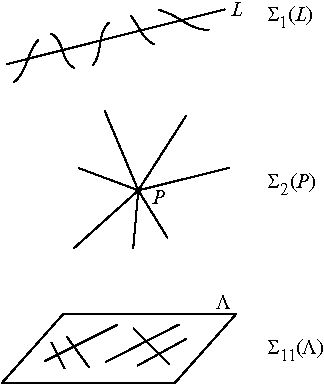
\includegraphics[height=2.7in]{main/Fig12-2}}
\caption{
Schubert cycles in $G(2,4)$:
$\Sigma_{1}(L)$
consists of
lines meeting $L\subset\PP^3$
(top);
$\Sigma_{2}(p)$
consists of
lines passing through $p\in\PP^3$
(middle);
$\Sigma_{1,1}(\Lambda)$
consists of
 lines in the plane $\Lambda\subset
\PP^3$
(bottom).
}
\label{Schubert cycles in G(2,4)}
\end{figure}

Figure~\ref{Schubert cycles in G(2,4)} illustrates some of
the possibilities for lines in $\PP^3` `$.

In particular, if $\sV(p)$ is the vanishing flag for forms of degree $d$
at a point $p\in \PP^{1}$, then
a $\grd$ has ramification sequence (termwise) $\geq \balpha$ at $p$
\index{ramification sequence}%
if and only~if $W$ belongs
to the Schubert variety $\Sigma_{\bbeta}(\sV(p))$, where $\beta_{i} =
\alpha_{\ell-i}$ as above.

For example, the Schubert cycle $\Sigma_{0,\dots,0}$ is the whole
Grassmannian,
\index{Grassmannian}%
and $\Sigma_{1,0,\dots,0}(\cal V)$ is the set of $\ell$-planes that meet
$V_{e-\ell}$ nontrivially, which is
a hyperplane section of the Grassmannian in its 
Pl\"ucker embedding.
\index{Pl\"ucker embedding}%
More generally, the
\emph{special Schubert cycle}
\index{special Schubert cycle}%
\index{Schubert cycle!special}%
$\Sigma_\gamma(\sV) \colonequals  \Sigma_{\gamma,0,\dots, 0}(\sV)$
is the set of $\ell$-planes
meeting  $V_{\gamma-\ell - \beta+1}$ nontrivially.
Since this condition really involves only the single space $U =
V_{e-\ell-\gamma+1}$, we sometimes
 write it
as $\Sigma_\gamma(U)$.

For any Schubert index $\bbeta$, the codimension of $\Sigma_{\bbeta}({\cal
V})$ in $G(\ell, e)$ is $|{\bbeta}|\colonequals  \sum \beta_i$
(Exercise~\ref{codim Schubert}).


\subsection*{Special Schubert cycles and Pieri's formula}

\begin{fact}
The variety of complete flags in $\CC^e$ is rational, and it follows
\index{Schubert cycle!special}%
that the class of $\Sigma_{\bbeta}({\cal V})\subset G$
in the 
Chow ring
\index{Chow ring}%
$A^*(G(\ell, e))$ of the 
Grassmannian
\index{Grassmannian}%
is independent
of the flag $\sV` `$. It is typically denoted $\sigma_{\bbeta}$. Moreover,
the classes $\sigma_{\bbeta}$ form a basis for the Chow ring as a free
abelian group.
\end{fact}

Thus the product $\sigma_\bbeta 
\cdot \sigma_{\smash{\bbeta'}\vphantom\beta}$  % align beta and beta'
is a linear
combination of Schubert classes,
given combinatorially by the \emph{Littlewood--Richardson rule}\emdash see
\index{Littlewood--Richardson rule}%
for example \cite{MR2247964}.
\emph{Pieri's formula} 
\index{Pieri's formula}%
is the special
case of the Littlewood--Richardson rule that expresses the product in
the Chow ring $A^*(G(\ell, e))$ of a special Schubert class with an
arbitrary Schubert class.
In Chapter~\ref{BrillNoetherproofChapter} we will use it to describe
the possible ramification behavior of rational curves with cusps.

\begin{proposition}[Pieri's formula]
\label{Pieri}
If $\sigma_\gamma$ is a 
special Schubert class
\index{Schubert class!special}%
and $\sigma_{\bbeta}$
is an arbitrary Schubert class, then
\index{Schubert class!product of --es}%
$$
\sigma_\gamma \cdot \sigma_{\bbeta} \; = \; \sum \sigma_{\bdelta}
$$
where the sum ranges over all Schubert indices ${\bdelta} = (\delta_1,
\dots \delta_{\ell})$ with
$$
\sum \delta_i = \gamma + \sum \beta_i \quad \text{and} \quad \beta_i
\leq \delta_i \leq \beta_{i-1}\quad \text{ for all } i
.
$$
\end{proposition}

For a proof, see for example \cite[Section 4.2.4]{3264}.

Figure~\ref{intersection product} illustrates the degeneration of
$\Sigma_1\cdot \Sigma_1$ to $\Sigma_2 \cup \Sigma_{1,1}$.

\begin{figure}[b]
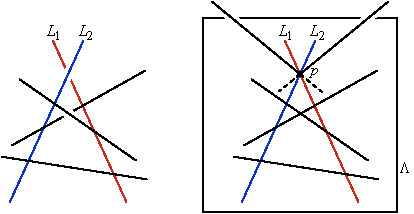
\includegraphics[height=1.8in]{main/Fig12-3}
\caption{When the lines $L_1$ and $L_2$ move to meet each other at $P$
they become coplanar in $\Lambda$,
and the intersection $\Sigma_1(L_1) \cap \Sigma(L_2)$
degenerates to the union $\Sigma_2(P) \cup \Sigma_{1,1}(\Lambda)$.
}
\label{intersection product}
\end{figure}

To understand Proposition~\ref{Pieri}, represent the Schubert class
$\sigma_{\bbeta}$ by 
stacks of coins,
\index{stacks of coins}%
with $\beta_1$ coins in the first
stack, $\beta_2$ coins in the second stack, and so on. We now want to
add a total of $\gamma$ coins to the stacks; we can add any number of
them to any stack (including a stack that was previously empty), with
the one condition that the new height of each stack can't be larger than
the previous height of the stack to its left. This interpretation makes
the following corollary clear:

\begin{corollary}\label{intersection with sigma nonzero}
If $\sigma_\gamma$ is any special Schubert class, $\sigma_{\bbeta}$
is any Schubert class,
and $m\geq 0$ is an integer with $m \gamma + \sum \beta_i \leq \dim
G(\ell, e) = \ell(e-\ell)$, then
$$
(\sigma_\gamma)^l \cdot \sigma_{\bbeta} \neq 0 \in A^*(G(\ell, e), \ZZ).
$$
\end{corollary}

The next result is expressed in terms of the \emph{osculating flag}
\index{osculating flag!defi}%
$\sV = 0\subset
V_1\subset \cdots \subset V_d = \PP^d$
to the rational normal curve $C\subset \PP^{d}$ at a point $p\in C$, which
we will now define. 

\def\tL{\,\widetilde{\!W\!}\,} % avoid superwide tilde
\def\tsV{{\widetilde \sV}}
\def\tV{{\widetilde V}}

Let $\tsV = (\tV_1, \dots, \tV_{d+1})$ be the 
 ramification flag defined previously (leaving
out $\tV_{0}$, which corresponds to the empty projective space), 
and let $V_{i}$ be the projectivization of $\V_{i+1}$. That is,
$V_{i}$ is the projective subspace of dimension $i$ that meets $C$ at $p$
with maximal order of contact.

\begin{proposition}\label{ramification}
Let $C \subset \PP^d$ be a rational normal curve, and $(V_W, \sO_C(1))$
be the $g^r_d$ on $\PP^1$ cut by hyperplanes in $\PP^d$ containing a
plane $W \subset \PP^d$ of dimension $d-r-1$, and write $\sV = 0\subset
V_1\subset \cdots \subset V_d = \PP^d$ for the 
osculating flag
of $C$
at $p$. The ramification sequence $\alpha(V_W, p)$
\index{ramification sequence}%
is determined by the formula
%
$$
W \in \Sigma_{\bfa}({\cal V}) \; \iff \; \alpha_i(V_W, p) \geq
\bfa^*_{r+1-i} = \#\{j\mid a_j\geq r+1-i\}.
$$
\end{proposition}

In other words, the ramification sequence $\alpha(V_W, p)$ of the linear
series $V_W$ at $p$ is exactly the reverse of the transpose of the
Schubert index of the smallest Schubert cycle containing $\tL$, the vector
space associated to $W` `$, in  $G(d-r, d+1)$.

\begin{proof}

The condition $\tL \in \Sigma_{\bfa}({\tsV})$
 means that
$$
\dim \tL \cap \tV_{r+1+i-a_i} \geq i
$$
for each $i$.
It follows that the codimension of the space of hyperplanes containing
$\tL$ has codimension $\leq r-a_i+1$.
since the projective space corresponding to $\tV_{r+i-a_i}$ is the linear
span of the divisor $(r+i-a_i+1)p\subset C$,
a codimension $\leq r-a_i+1$ space of sections of $\tV_{\tL}$  vanishes
to order $\geq r -a_i+1+i$ at $p$.

If we write the distinct orders of vanishing of the sections in
$\tV_{\tL}$ as
$b_0 < b_1<  \cdots < b_r$, we see that $\tL \in \Sigma_{\bfa}$  if
and only~if
$a_i$ of the $b_j$ are $\geq r+i+a_i+1$, that is,
$b_{r-a_i+1}\geq r-a_i+1+i$ or equivalently $\alpha_{r-a_i+1}\geq i$
for each $i$.
Since $\alpha_i\leq \alpha_{i+1} \leq \alpha_r$,
this is equivalent to saying that the number of $\{j \mid \alpha_j \geq
i\}$ is at least $a_i$, or, for the
reverse sequence $\alpha' = \alpha_r \geq \alpha_{r-1} \geq \cdots \geq
0$, that the $a_i$-th term is $\geq i$.
On the other hand $\bfa'_{a_i} = \#\{j\mid a_j \geq a_i\} = i$ since
the sequence $\bfa$ is weakly
decreasing, so $\alpha'$ is termwise $\geq \bfa'$.
\end{proof}

\subsection*{Conclusion}

Using these ideas we  can rephrase and prove Theorem~\ref{transversality
of ramification} in terms of Schubert cycles,
adding the precise condition for the existence of a $\grd$ with prescribed
ramification sequences
at an arbitrary collection of distinct points in $\PP^{1}$:

\begin{theorem}\label{osculating intersection}
Let $p_1,\dots,p_\delta \in C$ be distinct points on a rational normal
curve $C \subset \PP^d` `$, and ${\cal V}^1, \dots, {\cal V}^\delta$ the
corresponding vanishing flags. If ${\bbeta}^1, \dots, {\bbeta}^\delta$
are $\delta$ Schubert indices for $G(d-r, d+1)$, the Schubert cycles
$\Sigma_{{\bbeta}^1}({\cal V}^1), \dots, \Sigma_{{\bbeta}^\delta}({\cal
V}^\delta) \subset G(d-r, d+1)$ intersect properly; that is, the
intersection is either empty or has codimension exactly $\sum_{j
=1}^{\delta}|\bbeta^{j}|$,
the sum of the codimensions of the cycles $\Sigma_{{\bbeta}^j}$. Moreover,
the intersection is nonempty if and only~if
 the intersection product of the classes $[\Sigma_{{\bbeta}^j}]$ is
 nonzero in $A^*(G(d-r, d+1))$.
\end{theorem}


\begin{proof}
If the intersection is empty then the Chow class is 0, so it suffices
to show that the intersection is proper,
and we may assume that it is nonempty. Because the Grassmannian is smooth,
the codimension of the intersection of any subvarieties
 is at most the sum of their codimensions, so it is enough to show that
 the codimension of the
 intersection cannot be too small.

The Schubert cycle $\Sigma_1$ is a hyperplane section of the Grassmannian
$G(d-r, r+1)$, so that if $\Phi \subset G$ is any subvariety of
dimension $m$, its intersection with $m$ Schubert cycles $\Sigma_1$
is nonempty. Thus, if the intersection
$$
X \colonequals  \bigcap_{i=1}^\delta \Sigma_{{\bbeta}^i}({\cal V}^i)
$$
had dimension strictly bigger than the expected
$$
\rho \; \colonequals  \; (r+1)(d-r) - \sum_{i=1}^\delta |{\bbeta}^i|,
$$
we could choose $\rho + 1$ additional points $q_1,\dots,q_{\rho + 1}$
on $C$, with vanishing flags ${\cal V}^1, \dots, {\cal V}^{\rho + 1}$
and the intersection of $X$ with the Schubert cycles $\Sigma_1({\cal
V}^i)$ would still be nonempty.

It thus suffices to show that the intersection is empty if
$$
\sum_{i=1}^\delta |{\bbeta}^i| \; > \; (r+1)(d-r) = \dim G(d-r, d+1).
$$
If on the contrary
$$
W \; \in \; \bigcap_{i=1}^\delta \Sigma_{{\bbeta}^i}({\cal V}^i),
$$
then, by Proposition~\ref{ramification}, the linear series $(W,
\sO_{\PP^{1}}(d))$  would have
ramification of weight $|{\bbeta_i}|$ at $p_i$, and the sum of the
weights would be strictly greater than $(r+1)(d-r)$.
This contradicts the Pl\"ucker formula, Theorem~\ref{Plucker}.
\end{proof}

Using Proposition~\ref{ramification} this result becomes a
characterization of the sets of possible ramification
sequences for linear series at specified points on $\PP^1.$
 Explicitly, suppose we are given a collection of distinct points
 $p_1,\dots,p_\delta \in \PP^1` `$, and for each point $p_i$ a
 ramification sequence
$$
\alpha^i = (\alpha^i_0, \alpha^i_1, \dots, \alpha^i_r) \quad \text{with}
\quad 0 \leq \alpha^i_0 \leq \alpha^i_1 \leq \dots \leq \alpha^i_r
\leq d-r.
$$
Let ${\bbeta}^i$ be this sequence in reverse (and relabelled); that is
$$
{\bbeta}^i \; = \; (\alpha^i_r, \alpha^i_{r-1}, \dots, \alpha^i_1,
\alpha^i_0)
$$
and finally let $\bfb^i$ be the transpose of the Schubert index
${\bbeta}^i` `$.

\begin{corollary}
With $\alpha^i $ and $\bfb^i$ related as above,  there exists a
$g^r_d$ on $\PP^1$ with ramification sequence at $p_i$ equal to
$(\alpha^i_0, \alpha^i_1, \dots, \alpha^i_r)$ if and only~if
$$
\prod_{i=0}^\delta  \sigma_{\bfb^i} \; \neq \; 0 \quad \text{in} \quad
A^*(G(d-r, r+1)).
$$
\end{corollary}

\begin{proof}
If the product is nonzero, Proposition~\ref{ramification} and
Theorem~\ref{osculating intersection} immediately show the existence of
a $g^r_d$ on $\PP^1$ with ramification sequence greater than or equal
to $\alpha^i$ at $p_i$. But by Theorem~\ref{osculating intersection},
the ones with ramification strictly greater than the $\alpha^i$ form
a family of strictly smaller dimension. Thus a general $g^r_d$ with
ramification sequence greater than or equal to $\alpha^i$ at $p_i$
has  ramification sequence exactly equal to $\alpha^i$ at $p_i$.
\end{proof}

We can deduce a result about general secant loci
\index{secant flag}%
strengthening one that
was originally proven in \cite{Griffiths-Harris-BN}:
Given a curve $C \subset \PP^d` `$, we say that a \emph{secant flag}
in $\PP^d$ is a flag
$$
0 \subset V_1 \subset V_2 \subset \dots \subset V_{d-1} \subset V_d
= \PP^d
$$
where each $V_i$ is spanned by its (scheme-theoretic) intersection with
$C$. In other words, there is a sequence of points $p_1, p_2, \dots,
p_{d+1} \in C$ such that
$$
V_i \; = \; \overline{p_1+p_2+ \dots + p_{i+1}}
$$
(An osculating flag is just the special case where all $p_i$ are
equal.) Since any secant flag can specialize to an osculating flag,
we can deduce:

\begin{corollary}\label{secant schubert proper}
Schubert cycles defined relative to \emph{general} secant flags to a
rational normal curve intersect properly.
\end{corollary}

Unlike the case for osculating flags, the hypothesis of generality is
necessary for secant flags; see Exercise~\ref{only general secants}.

\section{Exercises}
\begin{exercise}\label{inseparable Gauss}
Let $k$ be a field of 
characteristic $p$.
\index{positive characteristic}%
Show that every point of the
affine curve $y = x^{p+1}+1$ over $k$ is a flex point.
\end{exercise}

\begin{exercise}\label{2g+2fixedpoints}
Show that if $C$ is a smooth projective curve of genus $g \geq 2$ and
$f : C \to C$ an automorphism fixing $2g+2$ points, then $C$ must be
hyperelliptic
\index{hyperelliptic}%
and $f$ the hyperelliptic involution.

Hint: Since we know that $f$ has finite order, we can take the quotient
$B = C/\langle f \rangle$ of $C$ by the cyclic group $\langle f \rangle$;
apply 
the Riemann--Hurwitz formula
\index{Riemann--Hurwitz formula}%
to the quotient map $C \to B$.
\end{exercise}

\begin{exercise}\label{curve in a product}
Suppose that $C\subset D\times E$ is a curve contained in the product
of smooth curves $D,E$ of genera $g$ and $h$ respectively.
Prove that if the degrees of the projection maps $C \to D$ and $C\to E$
are $d$ and $e$ respectively,
then
$$
p_a(C)\leq (d-1)(e-1) +dg+eh.
$$
Hint:  Use the Hodge index theorem~\ref{hodge index} and the adjunction
\index{Hodge index theorem}%
\index{adjunction formula}%
formula to show that the maximum possible genus of such
a curve $C$ is obtained when $C$ is linearly equivalent to a sum of
fibers of the two projections, in which case the inequality
becomes an equality.
\end{exercise}

\begin{exercise}\label{84(g-1)}
Show that if $C$ is a smooth projective curve of genus $g \geq 2$ then
$$
|\!\Aut C| \leq 84(g-1)
$$

Hint: Since we know that $\Aut C$ has finite order, we can take
the quotient $B = C/\Aut C$ of $C$; again, apply 
the Riemann--Hurwitz formula
\index{Riemann--Hurwitz formula}%
\index{automorphism group!size of}%
to the quotient map $C \to B$. (Warning: the idea is the same as in
Exercise~\ref{2g+2fixedpoints}, but the execution is substantially
more complicated.)
\end{exercise}


\begin{exercise}\label{codim Schubert}
Show that the codimension of $\Sigma_{\bbeta}({\cal V})$ in the
\index{Grassmannian}%
Grassmannian $G$ is equal to $\sum \beta_i$.

Hint: for $\Lambda \in \Sigma_{\bbeta}({\cal V})$, consider bases of
$\Lambda$ such that $\Lambda \cap V_i$ is the span of basis vectors.
\end{exercise}

\begin{exercise}\label{Schubert duality}
Let ${\bbeta}^*$ be
the transpose Schubert index to $\bbeta$.
\begin{enumerate}
\item  Show that $|\bbeta^*| = |\bbeta|$.
\item Show that $(\bbeta^*){\vphantom{\bbeta}}^* = \bbeta$. %align *s
\item Show that the isomorphism $\phi : G(k+1, V) \ruto{\,\cong} 
G(n-k, V^*)$ carries the Schubert cycle $\Sigma_\bbeta({\cal V})$ to the
Schubert cycle $\Sigma_{\bbeta^*}({\cal V}^*)$.
\end{enumerate}
(Of course, the first two parts follow from the third; think of the
first two as warmups.)
\end{exercise}

\begin{exercise}[ramification and osculating planes]\label{osculating
planes}
Let $p\in C\subset \PP^{d}$ be a point on a rational normal curve of
degree $d$, and
let $\Lambda\subset \PP^{d}$ be a $d-r-1$ plane, and let  $\sU
\colonequals (\sO_{\PP^{1}}(d), V)$
be
the  $\grd$,  possibly with basepoints, cut out by hyperplanes containing
$\Lambda$.
Consider the complete flag
$$
U(p) \colonequals  \{U_{1}, \dots, U_{d}\}
$$
of \emph{osculating spaces} at $p$, where $U_{t}$ is the linear span of
\index{osculating space}%
the divisor $tp$ considered
as a subscheme of length $t$ in $C$. Show that the ramification sequence
\index{ramification sequence}%
of $\sU$ at $p$
is determined by the formula
$$
W \in \Sigma_{\bfa}(U(p))
\; \iff \; \alpha_i(\sU, p) \geq \bfa^*_{r+1-i} = \#\{j\mid a_j\geq
r+1-i\}.
$$
In other words, the ramification sequence $\alpha(\sU, p)$ of the linear
series $\sU$ at $p$ is the reverse of the transpose of the Schubert
index of the smallest Schubert cycle containing $L$, the vector
space associated to $\Lambda$, in  $G(d-r, d+1)$. Conclude from
Theorem~\ref{osculating intersection}
that any collection of Schubert cycles associated to osculating flags
of $C$ at distinct points have intersection
that is dimensionally transverse or empty.
\end{exercise}

\begin{exercise}\label{independent secants 0}
Let $C$ be the rational normal curve in $\PP^{r}$. And let $(p_{i},
q_{i})\in  C^{2}$ be $t$ pairs of points, all distinct.
For each $i$, let $S_{i}$ be the Schubert variety of $k$-planes in
$\PP^{r}$ that meet the secant line
$\overline{p_{i}q_{i}}$. Show that if the $p_{i}, q_{i}$ are sufficiently
general, then the intersection
of the $S_{i}$ is dimensionally transverse. Hint: Let each pair of points
come together, and use the result
for the tangent lines, a special case of Theorem~\ref{osculating
intersection}.
\end{exercise}

\begin{exercise}\label{only general secants}
Show by example that Schubert cycles defined relative to arbitrary secant
flags to a rational normal curve may fail to intersect properly. (Hint:
it's enough to look at the case $d=2$ and $r=1$.)
\end{exercise}

\begin{exercise}
We can define the osculating flag to any nondegenerate curve $C \subset
\PP^d$ at any smooth point $p$. If $p$ is an inflection point then
$\overline{mp}$ may not be an $(m-1)$-plane, but we can look at the
nested sequence of subspaces
$$
\{p\} \subset \overline{2p} \subset \overline{3p} \subset \cdots
$$
and pick out exactly the terms whose dimension is strictly greater than
the preceding term; this gives a complete flag
$$
\{p\} \subset \overline{b_2p} \subset \overline{b_3p} \subset \dots
\subset \overline{b_{d+1}p} = \PP^d
.
$$
Show that the sum $\sum b_i - i$ is equal to the weight of the point $p$
as an inflection point of the hyperplane series.
\end{exercise}


\begin{exercise}
The Pl\"ucker formula shows that an elliptic normal curve $E\subset
\PP^{n-1}$ has $n^2$ inflection points. Show that they are
all simple, and that if you choose one as the origin for the group law
on $E$, then
they are the $n$-torsion points of  $E \cong Jac(E)$.

Hint: observe that the inflection points are the points $p \in E$ such
that $\cO_E(np) \cong \cO_E(1)$.
\end{exercise}

\begin{exercise}[Buchweitz]
It was long believed that every semigroup $H \subset \NN$ of finite index
\index{Weierstrass point)}%
$g = \#(\NN \setminus H)$ could occur as the Weierstrass semigroup of
a Weierstrass
point on a curve of genus $g$, but this is not the case. The following
counterexample for a curve of genus 16 was found by Buchweitz
\index{Buchweitz, Ragnar-Olaf}%
(unpublished): Show that on a curve of genus 16 there can be no
Weierstrass point $p$ with ramification sequence
$(0^{12}, 6,7,9,9)$ by showing that there would be too many vanishing
orders at $p$ of quadratic differentials.
 \end{exercise}

%footer for separate chapter files

\ifx\whole\undefined
\makeatletter\def\@biblabel#1{#1]}\makeatother
\gdef\urlhook{\url}
\bibliography{slag}
\bibliographystyle{msribib}


%%%% EXPLANATIONS:

% f and n
% some authors have all works collected at the end

\catcode`\^\active
%if ^ is followed by 
% 1:  print f, gobble the following ^ and the next character
% 0:  print n, gobble the following ^
% any other letter: print letter
\makeatletter
\def^#1{\ifx1#1f\expandafter\@gobbletwo\else
        \ifx0#1n\expandafter\expandafter\expandafter\@gobble\else#1\fi\fi}
\makeatother
\let\moreadhoc\relax
\def\indexintro{%An author's cited works appear at the end of the
%author's entry; for conventions
%see the List of Citations on page~\pageref{loc}.  
%\smallbreak\noindent
The letter `f' after a page number indicates a figure, `n' a footnote.}
\printindex[gen]
%requires makeindex
\end{document}
\else
\fi
 

\chapter{Proof of the Brill--Noether theorem}
\label{Brill Noether proof chapter}
\label{BrillNoetherproofChapter}

In this chapter we give a proof of the Brill--Noether
theorem based on the analysis
of inflections of linear series on $\PP^{1}$ of
Theorem~\ref{osculating intersection}. We will focus on proving what
we call the ``basic'' Brill--Noether theorem (Theorem~\ref{basic BN}),
which we reproduce for convenience:

\begin{theorem}[basic Brill--Noether]\label{BN-basic}
If
 $$
 \rho(g,r,d) \colonequals  g - (r+1)(g-d+r) \geq 0,
$$
then every smooth projective curve of genus $g$  possesses a
\index{g@$g^r_d$}%
$g^r_d$;
and for a general curve $C$,  $\dim W^r_d(C) = \rho$. Conversely, if
$\rho < 0$ then a general curve $C$ of genus $g$ does not possess a $g^r_d$.
\unif
\end{theorem}

In fact, a closer examination of our proof will yield some of the
assertions of the stronger Theorems~\ref{Wrd omnibus}
and~\ref{grd omnibus}, as well as additional results on the existence of
linear series with specified inflectionary behavior; we will discuss these at
the end of the chapter.

\section{Castelnuovo's approach}

The original argument of Brill and Noether reduced the proof to the
assertion that a matrix depending
on an invertible sheaf on a general curve
\index{Castelnuovo @Castelnuovo, Guido}%
behaves in a certain sense like a matrix of indeterminates. This was
finally proven in \cite{Griffiths-Harris-BN} using an idea that goes
\index{historical context}%
back to Castelnuovo \citeyear{zbMATH02692307}.

Interestingly, Castelnuovo's goal was not to prove the Brill--Noether
theorem, which was considered established at the time (or at least not
in need of further demonstration). Given that
a general curve of genus $2d-2$ has finitely many $g^{1}_{d}$s,
Castelnuovo asked: how many? We have answered this question in
the
cases $g = 2$, $4$ and 6 in earlier chapters,
and these cases were certainly known to Castelnuovo,
but the cases of higher $g$ were unknown.
His idea was to specialize to a general curve $C_0$ with $g$ nodes
whose normalization is $\PP^1` `$, and count the number of $g^1_d$s on
that curve. Appealing to the (then) vague ``principle of conservation
\index{principle of conservation of number}%
of number'', Castelnuovo felt that the result probably reflected the
number an a general smooth curve as well.%
%
\footnote{Castelnuovo
  presented his computation as heuristic, not claiming it was a full
  proof, and the reviewer of
his
paper in the \textit{Zentralblatt
f\"ur Mathematik}
\index{Zentral@\textit{Zentralblatt f\"ur Mathematik}}%
wrote very politely:
``Das Resultat, welches er bekommen hat, gibt mit grosser
Wahrscheinlichkeit den wahren Wert von $N$ \dots; daher sind wir mit dem
Verf.\ einverstanden, wenn er seinen Versuch nicht f\"ur wertlos h\"alt''
(The result that he obtained gives the true value of [the number of
$g^1_d$s] with high probability, and thus we agree with the author that
his work is not worthless\dots)}

By way of notation, we'll write $r_1,\dots,r_g$ for the nodes of
$C_0$, and let $p_i, q_i \in \PP^1$ be the two points lying over $r_i$.
Castelnuovo counted the $g^1_d$s on $C_0$ by observing that any pencil
on $C_0$ can be pulled back to a pencil on the normalization $\PP^1$;
if we embed $\PP^1$ in $\PP^d$ as a
rational normal curve
\index{rational!normal curve}%
of degree $d$, such a pencil is cut out by the hyperplanes containing
 a $(d-2)$-plane $\Lambda \subset \PP^d``$.
To say that such a pencil is a pullback from $C_0$ means that every
divisor of the pencil that contains $p_i$ contains $q_i$ and vice
versa. This  is equivalent to the condition that $\Lambda \cap
\overline{p_iq_i} \neq \emptyset$.

In the Grassmannian $G(d-1, d+1)$ of $(d-2)$-planes in $\PP^d``$,
the locus of those that meet the line $L_i = \overline{p_iq_i}$ is
what we called in the last chapter the Schubert cycle $\Sigma_1(L_i)$.
In these terms the set of $g^1_d$s on $C_0$ is the intersection
$$
W^1_d(C_0) \; = \; \tsty\bigcap\limits_{i=1}^{2d-2} \Sigma_1(L_i).
$$

Castelnuovo proposed that if the points $p_i, q_i\in \PP^1$ were chosen
generally, then the Schubert cycles
$L_i$ would meet transversely, and thus that the cardinality of this
intersection is the degree of the power $\sigma_1^{2d-2}$ in the
Chow ring
\index{Chow ring}%
$A(G(d-1, d+1))$. Castelnuovo evaluated this power, and came to
the conclusion that a general curve $C$ of genus $g=2d-2$ has
$$
\#W^1_{d+1}(C) \; = \; \frac{(2d-2)!}{(d-1)!@d!}
$$
pencils of degree $d$. Indeed, we see
 in Exercise~\ref{secant general position} that if the points $p_i, q_i$
 are general, then the Schubert cycles $\Sigma_1(L_i)$ at least intersect
 properly, so the given number is the number of $g^1_d$s counted with
 appropriate multiplicities.

Kleiman and Laksov \citeyear{MR323792,MR0357398} and
Kempf \citeyear{Kempf} used a
\index{Kleiman @Kleiman, Steven L.}%
\index{Laksov @Laksov, Dan}%
\index{Kempf @Kempf, George}%
different idea, which we'll describe
below, to prove the ``existence'' part of Theorem~\ref{BN-basic}
\emdash that is, that $W^{r}_{d}(C)$ is nonempty when $\rho\geq 0$.
In \cite{Kleiman-special}, the general ``nonexistence'' part is reduced
to the proof of Exercise~\ref{secant general position} and completed
for $r=1$. The general statement was finally proven in
\cite{Griffiths-Harris-BN}.

We will also adopt this general approach, and we will prove the existence
and nonexistence parts together
for all $g,d,r$. However, the strength of Theorem~\ref{osculating
intersection} compared to Exercise~\ref{secant general position} suggests
specializing to a $g$-cuspidal curve $C_0$ rather than a $g$-nodal one,
and we will use
this refinement.

\subsection*{Upper bound on the codimension of $W^r_d(C)$}
%\label{upper bound}

Let $C$ be a reduced irreducible projective curve of arithmetic genus
$g$.  In Section~\ref{BN by divisors} we showed how we might arrive
at the ``expected'' dimension of the locus
$W^r_d(C)$
\index{W@$W^r_d$}%
by estimating the
dimension of the subvariety $C^r_d \subset C_d$ of divisors moving in
an $r$-dimensional linear series; here we'll give a similar argument
using the
Picard variety
\index{Picard variety}%
$\pic(C)$. Again the heart of the proof is the
estimation of the
codimension of an
ideal of minors
\index{ideal!of minors}%
of a certain matrix of functions. Since
the proof uses degeneration
to a cuspidal curve, we will work with flat families of curves that may
include singular fibers. For simplicity
we will take the base of the family to be a complex disk $\Delta$
centered at the origin in $\CC$; the more algebraically minded reader
can substitute $\Spec$ of a
discrete valuation ring.

\begin{theorem}\label{local existence}
Let $\sC/\Delta$ be a family of reduced irreducible projective curves
of arithmetic genus $g$. If
the fiber  $C_0$ of the family has $\dim W^r_d(C_0) = \rho(g,r,d) \geq 0$
locally at a particular invertible sheaf $\sL_{0}$,  then $\dim W^r_d(C_b)
= \rho$ locally for all $b$ in a neighborhood of $0 \in \Delta$ and
invertible sheaves in a neighborhood of $\sL_{0}$
in the
relative Picard variety
\index{Picard variety!relative}%
$\pic_{d}(\sC/\Delta)$. In particular,
$W^r_d(C_b)$ is nonempty for all $b$ in a neighborhood of $0 \in \Delta$.
\unif
\end{theorem}

The idea of the following proof is a modern form of the discussion in
the original paper of Brill and Noether.

\begin{proof}  Possibly after pulling back the family $\sC/\Delta$
along a ramified covering $\Delta\to \Delta$
and restricting to a smaller disk around 0, we may choose $m$ sections
$p_{i}(b)$ with distinct values in the smooth locus of each fiber,
and $m$ as large as we like. We
define a family of divisors $D_{b} = \sum_{i}p_{i}(b)$.
By the
semicontinuity of fiber dimension,
\index{semicontinuity!of fiber dimension}%
we may choose $m$ so large
that $h^{1}(\sO_{C_{b}}(D_{b})) = 0$
and that for every invertible sheaf $\sL_{b}$ of degree $d$ on $C_{b}$
we have
$h^{1}(\sL_{b}(D_{b})) = 0$.
By Theorem~\ref{easy RR} we have
$$
h^0(\cL_{b}(D_{b})) =  d+m - g + 1.
$$
The pushforward of the
Poincar\'e sheaf
\index{Poincar\'e sheaf}%
$\cP$
on $\pic_{d+m}(\sC/\Delta)
\times \sC$ to $\pic_{d+m}(\sC/\Delta)$ is thus a vector
bundle $\sE$ of rank $d + m - g + 1$ on $\Delta$ whose fiber over a point
representing $\sL_{b}$ is the vector space $H^0(\cL(D_{b}))$. Similarly,
the pushforward
${\pi_1}_*(\cP|_{D_{b}})$
is a trivial vector bundle
\index{vector bundle}%
$\sF$ whose fiber at every point is the
$m$-dimensional vector space $\bigoplus_{i = 1}^{m} \cL(E)|_{p_i}$. Regarding
$D$ as a family of finite schemes inside $\sC$, the restriction map
$$
\cP  \to \cP_{D}
$$
pushes forward to give a map of vector bundles $\phi : \cE \to \cF$ on
$\sC$ which, on a fiber over $b$, is the evaluation of sections $\sigma
\in H^0(\cL_{b}(D_{b}))$ at the points $p_i$.

If $\cL_{b}$ is an invertible sheaf of degree $d$ on $C_{b}$ then
the space $H^0(\cL_{b})$ is the kernel of the map $\phi$ at the point
corresponding to $\cL_{b}(D_{b}) \in \pic_{d+m}(\sC/\Delta)$. Locally
on $\sC$ the map $\phi$ can be defined by a $(d+m) \times (d+m-g+1)$
matrix of regular functions. The locus $W^r_d(C_{b})$ is
thus the translate
by $\otimes \sO_{\sC}(D)$ of the locus where $\phi$ has rank $d+m-g-r$ or
less, and by \cite[Exercise 10.9]{Eisenbud1995} this locus is either empty
or its components have codimension $\leq (r+1)(g-d+r)$ in $\pic_{d+m}(C)$,
which has dimension $g$. Consequently, every component of $W^r_d(C)$
has dimension at least $\rho$.
\end{proof}

It was in fact this set-up that was used
by Kleiman-Laksov and Kempf
to prove the existence half of
Brill--Noether: they determined the characteristic classes of the bundles
involved and applied the
\index{Thom--Porteous formula}%
\emph{Thom--Porteous formula}, a formula for the
class of the degeneracy locus of a map of vector bundles. An account of
this proof is given in Appendix D of \cite{3264}.

We will see that if $C_{0}$ is any rational curve
with $g$ cusps, and $\rho(g,r,d)\geq 0$, then $\dim W^r_d(C_0) = \rho$
locally at every invertible sheaf on $C_{0}$.

\section{Specializing to a $g$-cuspidal curve}

Our first goal is to find a family $\{C_t\}$ of curves of arithmetic
genus $g$, with $C_t$ smooth for $t \neq 0$ and $C_0$ a rational curve
with $g$ cusps. To do this we show how to construct a rational curve $C_0$
with $g$ cusps and deform it to a smooth curve.

\subsection*{Constructing curves with cusps}

\begin{proposition}
Let $C$ be any curve and $p \in C$ a smooth point. There exists a curve
$C_0$ and a bijective morphism $f : C \to C_0$ such that  $f$ maps $C
\setminus \{p\}$ isomorphically to $C_0 \setminus \{r\}$ and the image
$r=f(p) \in C_0$ is a cusp of $C_0$.
\unif
\end{proposition}

We will say that we
\index{crimping}%
\emph{crimp} $C$ at $p$ to obtain $C_{0}$. For
the corresponding result with nodes instead of cusps, see
Exercise~\ref{independent secants}.

\begin{proof}
We can construct $C_0$ explicitly as a topological space homeomorphic
to $C$, with structure sheaf $\cO_{C_0}$ that is
the subsheaf of $\cO_C$ consisting of functions on $C$ whose derivative
at $p$ is 0.
\end{proof}

If we start with $\PP^1` `$, pick any $g$ points $p_1,\dots, p_g \in
\PP^1$ and crimp at each $p_i$, we arrive at a $g$-cuspidal curve $C_0$.


\subsection*{Smoothing a cuspidal curve}
Given a curve $C_0$ with a finite number of cusps and no other
singularities, we can find a proper flat family $\cC \to \Delta$ with
special fiber $C_0$ and all other fibers smooth;
that is, we can smooth $C_0$.

To begin with, we can do this locally in the complex analytic setting:
if $p \in C_0$ is a cusp, we can find an analytic neighborhood of $p$
in which $C_0$ is given by the equation $y^2 = x^3$; we can smooth this
by taking the family
$$
y^2 = x(x-t)(x-2t)
$$
for $t\in \Delta$.
(See Figure~\ref{Fig7.A}.)

The next step is to argue that we can glue together these local
smoothings
\index{smoothing}%
to obtain a proper family $\cC \to \Delta$, and this is where we need
to invoke a result from
deformation theory
\index{deformation theory}%
of projective schemes that
are
\index{locally complete intersection}%
locally complete intersections:

\begin{npt}
\begin{lemma}[{{\cite[Proposition 6.5.2]{MR2223408}}}]
\label{specialization to cuspidal curve}
Let
$p_1,\dots,p_g\in \PP^{1}$ be distinct points,
and let $C_0$ be
the curve
obtained by
crimping $\PP^1$ at each $p_i$. There exists a family of curves $\pi :
\cC \to \Delta$, where
\begin{enumerate}
\item $\Delta$ is a disk centered at the origin in $\CC$.
\item for all $b \neq 0 \in \Delta$, the fiber $C_b = \pi^{-1}(b)$
is a smooth, projective curve of genus $g$;  and
\item the fiber over $0$ is the curve $C_0$.
\unif
\end{enumerate}
\end{lemma}
\end{npt}

\begin{proof}[Sketch of proof]
The cuspidal curve $C_{0}$ can be embedded in projective space $\PP^{n}$
and there
it is locally a complete intersection.
Thus,
as with the case of one cusp,
above, the local obstructions
to smoothing vanish. The global obstruction is the first cohomology of
a sheaf supported at the cusps,
and therefore vanishes as well.
\end{proof}

\section{The family of Picard varieties}\label{Picard family}

By Lemma~\ref{specialization to cuspidal curve} there is a flat family
$\cC \to \Delta$ of curves, specializing from a smooth curve of genus
$g$ to a $g$-cuspidal curve. The next step is to relate linear series
on the general fiber of our family to their limits on $C_0$.

\subsection*{The Picard variety of a cuspidal curve}

\!We can describe the invertible sheaves on a cuspidal curve $C_{0}$
\index{cuspidal curve!$g$-}%
\index{cuspidal curve!Picard variety of}%
in terms of the invertible sheaves on its
normalization:

\begin{proposition}\label{torsion free on cuspidal}
Let $p\in C_{0}$ be a cusp that is the result of crimping a reduced
irreducible projective curve $C$ at a smooth point $q\in C$,
and let $\nu: C\to C_{0}$ be the natural morphism.
There is an exact sequence of groups
$$
0 \to (\CC,+) \to \pic_0(C_{0}) \ruto {\nu^*} \pic_0(C) \to 0.
$$
\end{proposition}

\begin{proof}
The preimage $\nu^{-1}(p)$ is the nonreduced scheme $2q \subset C$. If
$\cL$ is an invertible sheaf on
$C_{0}$ then $\nu^{*}(\cL)$ is invertible on $C$, and thus locally
trivial near $q$ and, in particular, trivial
when restricted to the subscheme $2q$. Conversely,
if $\cL'$ is an invertible sheaf on $C$ and we choose a trivialization
of $a: \cL'|_{U}\cong \sO_{U}$ on a neighborhood $ U\subset C$
of $q$, then there is an invertible sheaf $\cL$ on $C_{0}$ together with
a  trivialization
$a: \cL|_{\nu(U)}\cong \sO_{\nu(U)}$
on $\nu(U)$, unique up to an automorphism of $\sL'$ (that is, up to
multiplication by a scalar), that
pulls back to $\cL'$ with the given trivialization $a$.
Thus the data of an invertible sheaf $\cL$ on $C_0$ is equivalent
to the data of an invertible sheaf $\cL'$ on $C$, together with a
trivialization of $\widetilde \cL$ on the preimage $\nu^{-1}(p) = 2q$
up to multiplication by a nonzero scalar.

Of course every invertible sheaf on the
0-dimensional
scheme $2q$
is trivial, and a change of trivialization
thus corresponds to an automorphism of the structure sheaf $\sO_{2q}
\cong \CC[\epsilon]/(\epsilon^{2})$\emdash not as an algebra, but as a
rank 1 free module over $\CC[\epsilon]/(\epsilon^{2})$. Such a map is
determined by
its effect on the generator 1, and can take this element to any other
generator $a+b\epsilon$ with
$a\neq 0$ and $b\in \CC$ arbitrary. After multiplying $\sL'$ by $a^{-1}$
we may suppose that $a =1$ and we may take the automorphism to induce
the identity on $\CC$.
In this case, the family of trivializations, modulo multiplication by
a nonzero scalar, is
determined by the element $b\in \CC$.
Composing the isomorphisms
$1\mapsto 1+b\epsilon$ and $1\mapsto 1+b'\epsilon$  gives $1\mapsto
1+(b+b')\epsilon$,
so the kernel of the map $\nu^{*}: \pic_{d}(C_{0}) \to \pic_{d}(C)$ is
the additive group $(\CC, +)$.
\end{proof}

\begin{corollary}
If $C_{0}$ is a $g$-cuspidal rational curve, then $\pic_{d}(C_{0})
\cong \CC^{g}$. More precisely,
\index{rational!$g$-cuspidal curve}%
$\pic_{d}(C_{0})$ is a principal homogeneous space for the additive
group $\CC^{g}$, in the sense that
this group acts faithfully and transitively.
\unif
\end{corollary}

\begin{proof}
We can construct one invertible sheaf on $C_{0}$ as the inverse of the
ideal sheaf of a divisor of $d$ smooth points, and any other will differ
from this one by the choice of an element of $\pic_{0}(C_{0})$,
corresponding to a choice of $g$ trivializations, as in the proof of
the proposition.
\unif
\end{proof}

Thus we see that $\pic_{d}(C_{0})$ has dimension $g$ just as does the
Picard variety
\index{Picard variety}%
of a smooth curve
of genus $g$. An important difference is that $\pic_{d}(C_{0})$ is
not compact.

\subsection*{The relative Picard variety}

Returning to the family $\pi : \cC \to \Delta$ mentioned at the
start
\index{Picard variety!relative}%
of
Section~\ref{Picard family}, the Picard varieties $\Pic_d(C_t)$ form
a family $\pic_d(\cC/\Delta)$, and the varieties $W^r_d(C_t)$ form a
subfamily $\cW^r_d(\cC/\Delta)$.  In the argument
of Theorem~\ref{local existence} bounding  the dimensions of the $W^r_d$
we may replace the points $p_i$ by sections of the family, and thus
the codimension of $\cW^r_d(\cC/\Delta) \subset \pic_d(\cC/\Delta)$
is
at most
$(r+1)(g-d+r)$ locally at each point. See
Cheerful Fact~\ref{picard existence1}.

We will soon show that $W^{r}_{d}(C_{0})$, the fiber of
$\cW^{r}_{d}(\cC/\Delta)$ over 0,  is nonempty of dimension $\rho(g,r,d)$
when $\rho(g,r,d)\geq 0$ and otherwise empty. If the family of Picard
varieties over $\Delta$ were proper, so that limits of invertible sheaves
were invertible as in Figure~\ref{Fig13.1},
this would prove Theorem~\ref{BN-basic}; but it is not proper, and
thus it is a priori possible that $W^{r}_{d}(C_{0})=\emptyset$ but
$W^{r}_{d}(C_{t})\neq \emptyset$ for $t\neq 0$. This would mean that
families of invertible sheaves $\sL_{t}$ on $C_{t}$  simply don't
have  limits
in $\pic_{d}(C_{0})$. Indeed, the limit of a family of invertible sheaves
need not be an invertible
sheaf. Nevertheless we can describe these limits quite precisely.

\subsection*{Limits of invertible sheaves}
%\label{invertible sheaf limits}

Suppose  that  $\pi : \cC \to \Delta$ is a family of smooth genus $g$
\index{limit of invertible sheaves}%
curves specializing to a rational curve $C_0$ with $g$ cusps as in
Lemma~\ref{specialization to cuspidal curve}.
 Let
$$
\pi^\circ: \cC^\circ \colonequals  \cC \setminus C_0\to \Delta^\circ
\colonequals  \Delta\setminus 0,
$$
and suppose that there is a invertible sheaf $\cL^\circ$ on $\cC^\circ$
such that $h^0(\cL^\circ|_{C_b}) \geq r+1$ for each $b \neq 0 \in \Delta$
so that $\cL^\circ|_{C_b}\in W^{r}_{d}(C_{b})$. We would like to describe
the ``limit'' of $\sL$ as $b \to 0$.


\begin{lemma}\label{limit sheaf}
In the situation above, there exists a torsion-free sheaf $\cL$ of rank
\index{torsion-free sheaf}%
\1 on $\cC$, flat over $\Delta$ and locally isomorphic to
an ideal sheaf of $\cC$, such that $\cL|_{\cC^\circ} \cong\nobreak \cL^\circ$.
\unif
\end{lemma}

In fact, any torsion-free sheaf of rank 1 on $C_{0}$ is locally isomorphic
to an ideal sheaf; this follows from the fact that $C_{0}$ is generically
Gorenstein.
\index{Gorenstein}%
However, the argument we will give
shows directly that the extension is isomorphic to an ideal sheaf tensored
with an invertible sheaf, and the fact that
it is locally isomorphic to an ideal sheaf follows at once.

\begin{proof} Choose an auxiliary invertible sheaf $\cM$ on $\cC$ with
relative degree $e > d + 2g$ and let $\cM^\circ$ be the restriction of
$\cM$ to $C^\circ$. Consider the invertible sheaf
$$
\cN^\circ = (\cL^\circ)^* \otimes \cM^\circ.
$$

The bundle $\cN^\circ$ has lots of sections: the direct image, as a sheaf
on $B$, is locally free of rank $e-g+1 > 0$, and after restricting to
an open neighborhood of $0 \in B$ we can assume it's generated by them.

Choose a section $\sigma$ of $\cN^\circ$; let $D^\circ \subset \cC^\circ$
be its divisor of zeros, and let $D \subset \cC$ be the closure of
$D^\circ$ in $\cC$. Because it is the closure, the scheme $D$ has
no embedded
0-dimensional components, and thus $\sO_{\cC}/\sI_{D/\cC}$ has no
$\sO_{\Delta}$-torsion.

Since $\Delta$ is a smooth
curve, this implies that $\sO_{\cC}/\sI_{D/\cC}$ is flat over $\Delta$,
and thus $\sI_{D/\cC}|_{C_{0}}$
is an ideal sheaf, the kernel of $\sO_{\cC} \to
\sO_{\cC}/\sI_{D/\cC}$. Thus
$$
\cL \colonequals  \cI_{D/\cC} \otimes \cM
$$
has the desired properties.
\unif
\end{proof}

\begin{figure}
\centerline {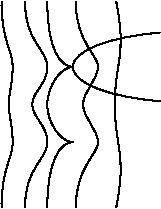
\includegraphics[height=2in]{main/Fig13-1}}
\caption{Cartier divisor on a smooth total space of a family of curves
that degenerates to a cuspidal curve; in this case the
limit of the associated family of invertible sheaves is invertible.}
\label{Fig13.1}
\end{figure}

Fortunately the ideal sheaves on cuspidal curves have a simple local
\index{ideal!sheaf}%
\index{cuspidal curve!ideal sheaf on}%
structure. The reason lies in the relation of the local ring $R_{0}$
of a cusp to its integral closure.

\begin{definition}
The \emph{conductor} of an integral domain $R_{0}$ is the annihilator
\index{conductor}%
of the $R_{0}$-module
$R/R_{0}$, where $R$ is the integral closure of $R_{0}$.
\unif
\end{definition}

It follows at once from the definition that the conductor of $R_{0}$
is also an ideal of $R$, and that it is the largest ideal of $R_{0}$
that is also
an ideal of $R$. The following result is a restatement of Example 2
after Proposition~\ref{Leray}:

\begin{proposition}\label{conductor of node and cusp}
If $R_{0}$ is the local ring of an ordinary cusp singularity of a curve,
then  $R/R_{0} \cong k$, the residue field of $R$, and thus the conductor
of $R_{0}$ is the
maximal ideal $\gm_{0}$ of $R_{0}$. \qed
\unif
\end{proposition}

\begin{proof} These properties can be verified after completing at the
maximal ideal of $R_{0}$.
To say
that $R_0$ has an ordinary cusp singularity means that the completion of
$R_0 \subset R$ is $k\[x^2,x^3\]\subset k\[x\]$, and the quotient is
$kx \cong k$.
\end{proof}


\begin{theorem}\label{torsion free at node}
Let $p$ be an ordinary cusp of a curve $C_0$ with normalization $\pi:
C \to C_0$. Let $R_0 = \sO_{C_0,p}$ be the local ring of the cusp,
with maximal ideal $\gm_0 = \sI_{p}R_{0}$,
and let $R_{0}\ruto {\pi^{*}} R$ be its normalization.  If $I_{0}\neq 0$
is an ideal of $R_{0}$ then
either $I_{0}\cong R_{0}$ or $I_{0}\cong \gm_0$.

 In the latter case, $I_{0} \cong Ra$, and if $R_{0}/I_{0}$ has length
 $v$ then $R/RI_{0} = R/I_{0}$ has length $v+1$.
 Moreover,
there is a split exact sequence
$$
0\to R/\gm_0 R \to R \otimes I_{0}  \to R I_{0} \to 0
$$
with $RI_{0}  \cong R$.
\unif
\end{theorem}

Interpreting Theorem~\ref{torsion free at node} in the context of an
ideal sheaf on a cuspidal curve
we get:

\begin{corollary}
Let $p\in C_{0}$ be an ordinary cusp in a reduced irreducible curve and
let $\pi:C \to C_{0}$ be
the partial normalization of $C_{0}$ at $p$, so that $p_a(C) = p_a(C_{0})-1$.
\index{partial normalization}%
Let $q\in C$ be the point lying over $p\in C_{0}$.

If $\sF_0$ is locally
isomorphic to a nonzero ideal sheaf on $C_{0}$
and $\sF_0$ is not locally free at $p$, then there is
a unique locally free sheaf $\sF$ on $C$ and a short exact sequence
$$
0\to \sO_{\pi^{-1}(p)} \to \pi^{*} \sF_{0} \to \sF \to 0.
$$
Thus $\chi(\sF) = \chi(\sF_{0}) -2$, so
$$
\deg@ \sF = \chi(\sF) - \chi(\widetilde \sO_{C}) =
\deg@\sF_{0}-1.
$$
Moreover, the map $H^{0}(\sF_{0}) \ruto {\pi^{*}} H^{0}(\sF(-q))$ is
a monomorphism.
\qed
\end{corollary}

\begin{proof}[Proof of Theorem~\ref{torsion free at node}]
The endomorphism ring of $I_0$ is commutative, it contains $R_0$,  and
\index{endomorphism ring}%
(since it stabilizes the finitely
generated module) it is integral over $R_0$. Thus
\index{integral endomorphism ring}%
$$
R_0 \subset \End I_0 \subset R.
$$
Since
$R/R_0 \cong k$, the ring $\End I_0$ is equal to either
$R_0$ or $R$.

First, suppose
$\End I_{0}=R$, which is a discrete valuation ring. Every ideal of $R$
is principal, so we may write $I_{0} = Ra$.
 Since $\gm_0$ is also an ideal of $R$, it is isomorphic to $R$
as an $R$-module, and since $R_0\subset R$,
$I \cong \gm_0$ as $R_0$-modules.
After completing we have
$\widehat R_{0} \cong \CC\[t^{2}, t^{3}, \dots\]$ and it is evident
that if $a$ has valuation $d$ in $R$ then the length of $R_{0}/(aR)$
is $d-1$, proving the claims in this case.

On the other hand, suppose
$\End I=R_0$
 and consider the inclusions
$$
\gm_0 I \subset I \subset R I.
$$
The left- and right-hand modules both have endomorphism ring $R$,
so both containments must be strict. Since $R/\gm_0$ has length 2,
we see that $I/\gm_0 I$ is principal. By
Nakayama's lemma
\index{Nakayama's lemma}%
$I\cong R_0$.
\end{proof}

Returning once again to the family $\cC \to \Delta$ at the beginning
of Section~\ref{Picard family}, assume that for general $t$ the scheme
$W^{r}_{d}(C_t)\neq \emptyset$. After replacing $\Delta$ with a
ramified covering we may assume that
$\sW^{r}_{d}(\sC/\Delta) \to \Delta$ has a section, that is, an
invertible sheaf $\sL$ on $\sC$ such that the restriction of $\sL$ to
each fiber $C_{t}$ with $t\neq 0$ has at least $r+1$ sections, so the
$g$-cuspidal curve $C_0$ that is the limit of this family has a
torsion-free sheaf $\cL_0$ of degree $d$. By the semicontinuity of
\index{semicontinuity!of cohomology}%
cohomology, $\sL_{0}$ also has at least $r+1$ sections.

At each cusp $r_i$ of $C_0$, $\cL_0$ is either locally free or
isomorphic to the maximal ideal of the cuspidal curve. Thus, if we
denote by $p_1,\dots, p_k$ the cusps of $C_0$ at which $\cL_0$ is
isomorphic to the maximal ideal, and let $C'_{0}$ be the partial
normalization of $C_0$ at those cusps, then $C'_{0}$ is a curve of
arithmetic genus $g-k$ having $g-k$ cusps, and the pullback of $\cL_0$
to $C'_{0}$ has at least $r$ sections with basepoints at the points
lying over $p_1,\dots,p_k$;  this is a $g^r_{d-k}$ on the
$(g-k)$-cuspidal curve~$D_0$.

\section{Putting it all together}
\label{nonexistence}

\subsection*{Nonexistence}

We can now prove that if $\rho(g,r,d) < 0$  then $W^{r}_{d}(C) =
\emptyset$ for curves in an open dense subset of $M_{g}$\emdash that is,
a general curve of genus $g$ does not possess a $g^r_d$.
Here we use Theorem~\ref{osculating intersection} from the last chapter,
which implies exactly this statement for invertible sheaves on an
arbitrary $g$-cuspidal curve $C_0$. If it were the case that a general
curve
had
a $g^r_d$ with $\rho(g,r,d) < 0$, then by the results
of Section~\ref{Picard family}, there would be
 an invertible sheaf of degree $d$ with $\geq r+1$ sections on a
 $(g-k)$-cuspidal curve  $ C'_0$ for some $k \geq 0$. But since
$$
\rho(g-k, r, d-k) = \rho(g,r,d) - k < 0
,
$$
this is impossible by Theorem~\ref{osculating intersection}.

\subsection*{Existence}

Once more we let $\cC \to \Delta$ be a family of smooth
curves specializing to a $g$-cuspidal curve $C_0$. We can
combine
Corollary~\ref{intersection with sigma nonzero} with
Theorem~\ref{osculating intersection} to
show
that the variety $W^r_d(C_0)$
is nonempty of dimension $\rho(g,r,d)$. Since the codimension of
$\cW^r_d(\cC/\Delta) \subset \pic_d(\cC/\Delta)$ is at most $(r+1)(g-d+r)$
locally everywhere, we may conclude, by the semi-continuity of fiber dimension, that likewise for general $t$
the variety $W^r_d(C_t)$ is nonempty of dimension exactly $\rho(g,r,d)$.

\section{Brill--Noether with inflection}

The approach we've taken here to the proof of Brill--Noether is
\index{linear series!on $\PP^1$, inflections of}%
\index{inflectionary!behavior}%
\index{Brill--Noether theorem!with inflection}%
well-suited to analyzing the inflectionary behavior of linear series on a
general curve; indeed, a small modification of the argument above allows
us to prove a stronger form of the Brill--Noether statement, concerning
the existence of $g^r_d$s on a general curve $C$ that are required to
 have inflection points of given weights.

\begin{definition}
Let $C$ be a smooth curve of genus $g$ and $p_1,\dots,p_n \in C$ distinct
points of $C$. If $\cD = (L,V)$ is a linear series on $C$ of degree $d$
and dimension $r$, we define the \emph{adjusted Brill--Noether number}
\index{Brill--Noether number!adjusted}%
of $\cD$ relative to the points $p_k$ to be
$$
\rho(\cD; p_1,\dots,p_k) \colonequals  g - (r+1)(g-d+r) - \sum_{k=1}^n
w(\cD,p_k).
$$
\end{definition}

In these terms, we can prove
a
generalization of the
``nonexistence'' half of Brill--Noether:

\begin{theorem}\label{Brill--Noether with inflection}
Let $(C;p_1,\dots,p_n)$ be a general $n$-pointed curve of genus $g$
\index{general $n$-pointed curve}%
\index{pointed curve}%
(that is, let $C$ be a general curve and $p_1,\dots,p_n \in C$ general
points). If $\cD$ is any linear series on $C$, then
$$
\rho(\cD; p_1,\dots,p_n) \geq 0.
$$
\end{theorem}

\begin{proof}
To start, let $\cC \to \Delta$ be a family of curves as in the proof of
Lemma~\ref{specialization to cuspidal curve}.
As in the argument
at the start of Section~\ref{nonexistence},
possibly
after pulling back the family along a ramified map $\Delta \to \Delta$,
we can choose sections $\sigma_1, \dots, \sigma_n : \Delta \to \cC$
of $\cC \to \Delta$ such that the $\sigma_k(0)$ are distinct smooth
points of $C_0$.
If the general curve $C_b$ in our family admits a $g^r_d$ $\cD$ with
$$
\rho(\cD;\sigma_1(b),\dots,\sigma_n(b)) < 0
$$
then, possibly after pulling the family back along a ramified map $\Delta
\to \Delta$, we can choose a family $\{\cD_b\}$ of such linear series
on the fibers $C_b$ for $b \neq 0$ and, taking limits, we arrive at a
$g^r_d$ $\cD_0$ on $\PP^1$ with
$$
w(\cD_0, q_i) \geq r
$$
for each of the $g$ points $q_i \in \PP^1$ lying over the cusps of $C_0$,
and in addition
$$
w(\cD_0, r_k) \geq w(\cD_b,\sigma_k(b))
$$
where $r_k \in \PP^1$ is the point in $\PP^1$ lying over $\sigma_k(0)
\in C_0$. Adding up, we have
\begin{align*}
\sum_{i=1}^g w(\cD_0, q_i) + \sum_{k=1}^n w(\cD_0, r_i) &\geq rg +
\sum_{k=1}^n w(\cD_b,\sigma_k(b)) \\
&> rg + g - (r+1)(g-d+r) = (r+1)(d-r)
,
\end{align*}
since we assumed that
$$
\rho(\cD_b;\sigma_1(b),\dots,\sigma_n(b)) = g - (r+1)(g-d+r) -
\sum_{k=1}^n w(\cD_b,\sigma_k(b)) < 0.
$$
But as before the Pl\"ucker formula for $\PP^1$ tells us that
$$
\sum_{p \in \PP^1} w(\cD_0, p) = (r+1)(d-r),
$$
a contradiction.
\end{proof}

This extension of the ``nonexistence'' part of
the Brill--Noether theorem
raises
the question of a converse: if $(C;p_1,\dots,p_n)$ is a general
$n$-pointed curve of genus $g$, and we specify ramification sequences
$\alpha^1, \dots, \alpha^n` `$, can we say that there exists a $g^r_d$
$\cD$ on $C$ with $\alpha_i(\cD, p_k) \geq \alpha^k_i$ for
$k=1,\dots,n$ and $i = 0, \dots, r$? If the product of the
corresponding
Schubert classes
\index{Schubert class}%
in $G(d-r, d+1)$ is nonzero, then we
can indeed deduce the existence of such a linear series; and if the
product is 0, we can deduce that no such linear series exists.

Here is one way to state what we know without getting lost in a thicket
of Schubert calculus:

\begin{theorem}\label{BN with inflection and dimension}
Let $C$ be a smooth curve of genus $g$ and $p_1,\dots,p_n \in C$ distinct
points; for $k = 1,\dots,n$ let $\alpha^k = (\alpha^k_0,\dots\alpha^k_r)$
be a nondecreasing sequence of nonnegative integers, and let
$$
G^r_d(p_1,\dots,p_n; \alpha^1,\dots,\alpha^n) = \{\cD \in G^r_d(C)
\mid \alpha_i(\cD, p_k) \geq \alpha^k_i \}.
$$
If $@(C, p_1,\dots,p_n)$ is a general $n$-pointed curve,
then either
$$
G^r_d(p_1,\dots,p_n; \alpha^1,\dots,\alpha^n)
$$
is empty, or it has dimension
$$
%\dim G^r_d(p_1,\dots,p_n; \alpha^1,\dots,\alpha^n) =
\rho(g,r,d) -
\sum_{k+1}^n \sum_{i=0}^r \alpha^k_i.
$$
\end{theorem}

Finally, from the codimensions of the Schubert varieties  we can deduce
the ramification behavior of general
linear series:

\begin{theorem}
If $\cD$ is a general $g^r_d$ on a general curve, then $\cD$ has only
\index{ramification!simple}%
\index{Weierstrass point}%
simple ramification; that is,
$$
w(\cD, p) \leq 1 \quad \text{for all } p \in C.
$$
\end{theorem}

Applying this in case $d=2g-2$ and $r = g-1$, we arrive at the
statement made
after Corollary~\ref{Weierstrass points}:
that a general
curve $C$ of genus $g$ has only Weierstrass points of weight 1.

\section{Exercises}

\begin{exercise}
  By Theorem~\ref{BN with inflection and dimension}, there is a $g^1_4$
  on a general curve $C$ of
genus 3
\index{g@$g^1_4$}%
\index{genus 3 curve}%
ramified at any 2 general points $p, q \in C$. Construct it.
\tohint{14.1}
\end{exercise}

The
next
three exercises give the results necessary to prove
Theorem~\ref{BN-basic} using degeneration to
nodal curves
\index{nodal curve}%
rather than to cuspidal curves.

\begin{exercise}[construction of nodal curves]
\label{independent secants}
\label{Constructing nodal curves}
Let $C$ be a smooth curve,
and let
 $\{(p_{i}, q_{i}) \mid i = 1\dots h\}$ be $2h$ distinct points of $C$.

Show that if $C$ is embedded in $\PP^{r}$ by a complete linear series
of sufficiently high degree, then the
projection of $C$ from a general $(r-4)$-plane $\Lambda$ that meets each
secant $\overline{p_{i} q_{i}}$
maps $C$ to a curve with $h$ ordinary nodes in $\PP^{3}$.
\tohint{14.2}
 \end{exercise}

\begin{exercise}\label{BN via nodal curves}\label{secant general position}
Suppose that $C\subset \PP^{d}$ is the rational normal curve of degree
$d$, and $\{L_{i} = \overline{p_{i}q_{i}}\}$
is a collection of secants of $C$. Show that if the points $p_{i},
q_{i}\in C$ are chosen sufficiently generally,
then any collection of Schubert cycles $\Sigma_{a_{i}}(L_{i})$ meet
dimensionally transversely.
\tohint{14.3}
\end{exercise}

\begin{exercise}\label{linear series on a nodal curve}
Imitate the proof of Proposition~\ref{torsion free on cuspidal} to
show that if $R_{0}$ is the local ring of a node\emdash that is, the
completion $\widehat R$ is isomorphic to $\CC[x,y]/(xy)$\emdash then
every nonzero ideal of $R$ is isomorphic
either to $R$ or to the maximal ideal of $R$. Deduce that if $C\to C_{0}$
is the
partial normalization of a single node on a reduced irreducible projective
curve, then there is an exact sequence
$0\to \CC^{*} \to \pic_{0}(C_{0}) \to \pic_{0}(C) \to 0$.
\tohint{14.4}
\end{exercise}



\chapter{Using a singular plane model}
\label{PlaneCurvesChapter}
\label{PlaneCurveChapter}


In the first part of Chapter~\ref{genus 1 chapter} we showed how to
use an embedding of a smooth curve $C$
in $\PP^2$ to understand differentials and linear series on $C$.
In that form,
the technique
has limited applicability,
since most smooth curves cannot be embedded in
$\PP^2$.
However, by Proposition~\ref{nodal projection},
 any smooth curve $C$ can be projected
birationally to a curve $C_0\subset\PP^2$ with only nodes.
We open this chapter by showing
how to use such a nodal model $C_0$ to describe differentials and
linear series on $C$, a theory well-understood
by Brill and Noether;  and then explain
what is necessary to adapt the technique to birational images of $C$
with arbitrary singularities.

\section{Nodal plane curves}\label{nodal curves section}

The methods of Chapter~\ref{3b}
 can be applied, with one change, when $C_{0}\subset \PP^{2}$
\index{nodal curve}%
is a nodal curve.

Let $\nu: C\to C_{0}\subset \PP^{2}$ be the
\index{normalization}%
normalization morphism from a smooth curve,
and let $B\subset C_{0}$ be a subscheme.
It will be convenient to speak of
\index{linear series!cut out by curves}%
\emph{the linear series cut out on $C$} by curves of degree $m$
containing $B$: though $B$ is only a subscheme, $\nu^{-1}(B)$ may be
considered as a
Cartier divisor
\index{Cartier divisor}%
 because
$C$ is smooth, and we define
the linear series cut out on $C$ by curves of degree $m$
containing $B$ to be
the linear series  $\sV$ of divisors in $C$ that are residual to $\nu^{-1}(B)$ in the pullbacks
of the intersections of $C_{0}$ with curves of degree $m$.
Formally, since $B' \colonequals  \nu^{-1}(B)$
is a Cartier divisor on $C$, we can say that if $L$ is the divisor of a line in $\PP^{2}$ and $L'$
its pullback to $C$ then
$\sV$ is a space of divisors corresponding to
sections of $\sO_{C}(mL'-B')$; more precisely, it is the space of divisors corresponding to
sections of $\sO_{C}(mL'-B')$ in the image of the restriction/pullback map
$$
H^0(\cI_{B/\PP^2}(m)) \to H^0(\sO_{C}(mL'-B')).
\unif
$$

\subsection{Differentials on a nodal plane curve}\label{canonical series on nodal plane curves}

Let $C_{0} \subset \PP^2$  be a curve of degree $d$ with $\delta$
nodes and no other singularities. By the
adjunction formula
\index{differential form!on nodal plane curve}%
\index{nodal curve!differential on}%
\index{adjunction formula}%
 (Proposition~\ref{adjunction}),
Proposition~\ref{pa and delta}, and the first example that follows it,
the genus $g$ of the normalization $C$ of $C_{0}$ is
the arithmetic genus $p_{a}(C_{0}) = \tbinom{d-1}{2}$
of $C_{0}$ minus $\delta$, that is,
$$
g = \mbinom{d-1}{2} -\delta.
$$
We will make this explicit by
\index{regular!differential}%
\index{differential!regular}%
exhibiting a vector space of $g$ regular differential forms on $C$.

Choose homogeneous coordinates  $[X,Y,Z]$ on $\PP^2$ so that
$C_0$ intersects the line $L = V(Z)$ in a divisor $D$ consisting only
of smooth points of $C_{0}$  other than $[0,1,0]$, and
so that at each node of $C_0$ (necessarily contained in the affine plane $U = \PP^2 \setminus L$) the tangents to $C_0$ have finite slope.
Let the nodes of $C_0$ be $q_1,\dots,q_\delta$, with $r_i, s_i \in C$ lying
over $q_i$; we'll denote by $\Delta$ the divisor $\sum r_i + \sum s_i$ on $C$.

Let $F(X,Y,Z)$ be the homogeneous polynomial of degree $d$ defining
the curve $C_0$, and let $f(x,y) = F(x,y,1)$ be the defining equation
of the affine part $C_{0}^{\circ}\colonequals  C_0 \cap U$ of $C_0$.
Let $\nu: C\to C_0$ be the normalization map. We start by considering
the rational differential
\index{rational!differential}%
$\nu^*(dx)$ on
$C^{\circ}\colonequals  \nu^{-1}(C_{0}^{\circ})$.

In the smooth case where $C_{0}=C$ we saw that this differential was
regular and nonzero on $C^{\circ}$; this followed from the fact
that $f_{x}$ and $f_{y}$ had no common zeroes on $C_0$. But now
$f_{x}$ and $f_{y}$ have common zeroes: they both vanish to order~1 at
the points $q_{i}$ and thus $\nu^*(f_{x})$ and $\nu^*(f_{y})$ have
simple zeroes at the points $r_i$ and $s_i$.

As before, the differential $\nu^*(dx)$
has  double poles along the divisor
$D$ on $C_{0}$ lying over the point at infinity in $\PP^{1}$
and we see that for a polynomial $e(x,y)$ of degree $\leq d-3$, the
differential
$$
\nu^*\left( \frac{e(x,y)\,dx}{f_{y}}\right)
$$
is regular except for simple poles at the points $r_i$ and $s_i$.

We can get rid of these poles by requiring that $e$ vanishes at the
points $q_i$. We say in this case that $e$ (and the curve defined by $e$)
 \index{conditions of adjunction}.
\emph{satisfies the conditions of adjunction}.

\begin{theorem}\label{canonical from adjoint 1}
If $C_{0}$ is a nodal plane curve of degree $d$ with normalization $\nu:
C\to C_{0}$
then the  regular differentials on  $C$, in terms of the notation above,
 are precisely those of the form
 $$
\nu^{*}\biggl( \frac{e(x,y)\,dx}{f_{y}}\biggr)
,
$$
where
$e(x,y)$ ranges over the polynomials of degree $\leq d-3$
vanishing at the nodes of $C_{0}$.

Thus if $\adj(C_{0})\subset C_{0}$ denotes the union
\index{F@$\adj(C_{0})$}%
of the reduced points at the nodes of $C$, then $|\omega_{C}|$ is the
linear series cut out on $C$ by
forms of degree $d-3$ containing $\adj(C_{0})$.
\unif
\end{theorem}

See Figure~\ref{canonical on normalization} for a picture in a case
where $C_0$ has a single node.
\begin{proof}
The dimension of the space of polynomials $e(x,y)$ of degree at most
$d-3$ is $\tbinom{d-1}{2}$,
and vanishing at $\delta$ nodes imposes at most $\delta$ linear conditions
on $e$. The linear map sending
$e\mapsto \nu^{*}(e\,dx/f_{y})$ is injective, and the target has dimension
$\tbinom{d-1}{2}-\delta$, so this must be an isomorphism.
\end{proof}
We will give a more conceptual proof of this theorem in
Section~\ref{arbitrary plane curves}.

In particular, Theorem~\ref{canonical from adjoint 1}
shows that the linear series cut out on $C$ by
forms of degree $d-3$ containing $\adj(C_{0})$ is complete. (We will
soon see that
 the linear series cut out on $C$ by
forms of degree $m$ containing $\adj(C_{0})$ is complete for every $m$.)


This gives another proof of Lemma~\ref{adjoint independent}.

\begin{corollary}
If $C$ is a nodal plane curve of degree $d$, then the nodes of $C_{0}$
impose independent
\index{independent conditions}%
conditions on forms of degree $d-3$.
\unif
\end{corollary}

\begin{proof}
 Otherwise the space of differential forms on the normalization of $C_{0}$
 would be too large.
\end{proof}

One can use Theorem~\ref{canonical from adjoint 1} to re-embed a plane
curve of
geometric genus $g$ as a
canonical curve
\index{canonical curve}%
in $\PP^{g-1}$:

\begin{corollary}
 The canonical ideal of the normalization of a nodal plane curve of
 degree $d$ is the ideal of polynomial relations
 among the forms of degree $d-3$ that vanish at the nodes of the
 curve. \qed
\end{corollary}

\begin{figure}
\centerline {\includegraphics[width=3in]{"main/Fig14-2"}}
\caption{A curve $C$ of geometric genus 2 represented as the normalization
of a plane curve $C_{0}$ of degree 4 with a node, and a canonical divisor,
represented by a conic containing the node.}
\label{canonical on normalization}
\end{figure}

\subsection{Linear series on a nodal plane curve}
\label{linear series on nodal plane curves}

Since $C_{0}$ is singular, not every
effective divisor
\index{effective divisor}%
on $C$ is the
\index{linear series!on nodal plane curves}%
preimage of an
effective Cartier divisor on $C_{0}$. As an example, one may take a
single point lying over a node
as in Figure~\ref{Fig14.2}.

However,
we can still represent every divisor on $C$ as the preimage of a divisor
on $C_{0}$ up to linear
equivalence, and the same goes for any reduced curve:

\begin{lemma}
Let $\nu: C\to C_{0}$ be the normalization of any reduced projective
\index{normalization}%
curve. If $D$ is any divisor
on $C$, then $D$ is linearly equivalent to the pullback of a divisor
supported on the smooth locus of  $C_{0}$. More precisely,  every
effective divisor on $C$ containing $\Delta$ can be written as the
pullback
of a
Cartier divisor
\index{Cartier divisor}%
on $C_{0}$.
\unif
\end{lemma}

We will see a more general version in Theorem \ref{Cartier on C}.

\begin{proof}
It suffices to prove the result locally on $C_{0}$, where it is
geometrically obvious:  if the node
$p\in C_{0}$ has preimages $q,r$ corresponding to  branches $Q$ and $R$ of $C_{0}$
at $p$, then
a divisor $aq+br$ with both $a,b$ strictly positive, is locally the
pullback of the intersection of $C_{0}$
with a curve $C'$ meeting $Q$ with multiplicity $a$  at $p$ and meeting $R$
with multiplicity $b$ at $p$. For example, assuming that $a\leq b$, we could take
$C'$ to be the union of $a-1$ general lines through $p$ and a smooth plane curve
meeting $R$ with multiplicity $b-a+1$ at $p$.
\end{proof}


Returning to the case of a nodal plane curve $C_{0}$ and its normalization
$\nu: C\to C_{0}$,
suppose that $D$ is a divisor on $C$ that is the pullback of a difference
of Cartier
divisors $D_{+}-D_{-}$ on $C_{0}$. We will compute the complete linear
series $|D|$.
Let $\adj(C_{0})$ be the set of nodes in $C$ and let $\Delta$ be the
preimage of $\adj(C_{0})$ in $C$.

\begin{theorem}\label{linear series on nodal curves}
Let $D = D_{+}-D_{-}$ be a divisor on $C$, and let $G$ be a form on
$\PP^{2}$
that vanishes on  $D_{+}+\adj(C_{0})$ but not identically on $C_{0}$.

If $G$ has degree $m$ and $A = (\nu^{*}G)-D_{+}-\Delta$, then every
effective divisor on
$C$ linearly equivalent to $D$ (if any) has the form
$(\nu^*H)-D_{-}-A-\Delta$ for some $H$ of degree $m$
that vanishes on $\adj(C_{0})+A$ but not identically on $C_{0}$.
\unif
\end{theorem}

The reason for including $\adj(C_{0})$ is that an arbitrary linear series on $C$
cannot be represented as the pullback of a linear series on $C_{0}$ without this.
We will see a generalization in Theorem \ref{linear series on arbitrary curves} and the surrounding discussion.

\begin{corollary}
With notation as in Theorem~\ref{linear series on nodal curves}, the
ideal of the image of
$C$ with respect to the linear series $|D|$ is the ideal of polynomial
relations among the forms
of degree $m$ in $\ff_{C/C_{0}}$ that vanish on $D_{-}+ A$.\qed
\unif
\end{corollary}

\begin{proof}[Proof of Theorem~\ref{linear series on nodal curves}]
 Choose an integer $m$
big enough
that there is a form $G$ vanishing
 on  $D_{+}$ and $\adj(C_{0})$ so that
 $\nu^{*}(G)$ vanishes on $D_{+}+\Delta$, but not everywhere on $C$.
 (If $D_{+}$ contains some positive multiple of a point $p$ of $\Delta$
 this means that $G$ defines
 a curve sufficiently tangent to the corresponding branch of $C_0$.)
Then, as before,
we can write the zero locus of $G$ pulled back to $C$ as
$$
(\nu^*G) = D_{+} + \Delta + A.
$$

\begin{figure}
\centerline {\includegraphics[width=3.0in]{"main/Fig14-3"}}
\caption{If $G$ is tangent to a branch of $C_{0}$ at the node, then
$D_{+}$ contains
a point of $\Delta$ on $C$.}
\label{Fig14.2}
\end{figure}

Next, we look for forms $H$ of the same degree $m$, vanishing at $A+D_{-}$
and on $\adj(C_{0})$
 but not on all of $C_0$. If there are no such polynomials $H$ then,
 as we shall show,
there are no effective divisors equivalent to $D$. Supposing that there
is such a form $H$, let $D'$ be the divisor
$$
D' = (\nu^*H) -( D_{+} + \Delta),
$$
that is, $D'$ is residual to $( D_{+} + \Delta)$ in $(\nu^*H)$.

Since $\nu^*(G/H)$ is a rational function on $C$ we have
$$
D_{-} +\Delta + A+ D' = (\nu^*H) \sim (\nu^*G) = D_{+} + \Delta + A,
$$
and thus $D'$ is an effective divisor linearly equivalent to $D =
D_{+}-D_{-}$ on $C$.

To complete the argument we must show that we get \emph{all} divisors $D'$
in this way.
In this case the curve $C$ can be desingularized by blowing up the plane
once at each node,
and we can give a proof based on the resulting surface $S$. The same
technique would work for any curve with only
\index{ordinary multiple points}%
\index{total transform}%
\index{normal!crossing}%
ordinary multiple points, in which case the total transform of $C_{0}$ on
$S$ has normal crossings. We will give a different proof, extending this
theorem to curves with arbitrary singularities, in Section~\ref{arbitrary
plane curves}.

\begin{proposition}\label{adjoint completeness1}
If $C_{0}$ is a reduced irreducible plane curve all of whose singularities
are ordinary nodes, then for each
integer $m$,
the linear series cut out on the normalization $C$ of $C_{0}$ by forms
of degree $m$ containing the nodes
is complete.
\end{proposition}

\begin{proof}
To prove Proposition~\ref{adjoint completeness1}, we work on the blowup
$\pi : S \to \PP^2$ of $\PP^2$ at the nodes $q_i$ of $C_0$. The proper
transform of $C_0 \subset \PP^2$ in $S$ is the normalization of $C_0$,
\index{normalization}%
which we will again call $C$.

Let $L$ be the class on $S$ of the pullback of a line in $\PP^2$
and let $E$ be the sum of the exceptional divisors, the preimage of
$\adj(C_{0})$. We write $h= L\cap C$ and $e = E\cap C= \sum (p_i+q_i)$
for the corresponding divisors on $C$.
Because $C$ has double points at each $q_{i}$ we have
$
C \sim dL - 2E
$
and   by
Theorem~\ref{divisor classes on blowup} we have $K_S \sim -3L + E$.

The proper transform of a degree $m$ curve $A\subset \PP^2$  passing
simply through the points $q_i$
is $\pi^*A - E$; this gives an isomorphism
$$
H^0(\cI_{\{q_1,\dots,q_\delta\}/\PP^2}(m)) \cong H^0(\cO_S(mL-E)).
$$
In these terms we can describe the linear series cut on $C$ by plane
curves of degree $m$ passing through the nodes of $C_0$ as the image of
the map
$$
H^0(\cO_S(mL-E)) \to H^0(\cO_C(mL-E)),
$$
and we must show that this map is surjective.

From the long exact cohomology sequence associated to the exact sequence
of sheaves
$$
0 \to \cO_S((m-d)L + E)  \to \cO_S(mL-E) \to \cO_C(mL-E) \to 0,
$$
 we see that it will suffice to prove that $H^1(\cO_S((m-d)L + E)) = 0$.

By Serre duality on $S$,
$$
H^1(\cO_S((m-d)L + E)) \cong H^1(\cO_S((d-m-3)L))^*.
$$
The line bundle $\cO_S((d-m-3)L)$ is
 the pullback to $S$ of the bundle $\cO_{\PP^2}(d-m-3)$, which has
 vanishing $H^1` `$. Lemma~\ref{H1 on pullback} completes the proof.
\end{proof}

\begin{lemma}\label{H1 on pullback}
Let $X$ be a smooth projective surface, and $\pi : S \to X$ the
\index{blowup}%
blowup of
a finite set of reduced points. If $\cL$ is any line bundle on $X$, then
$$
H^1(S, \pi^*\cL) = H^1(X, \cL).
$$
\end{lemma}

\begin{proof} Because $\PP^2$ is normal, and $\pi_*(\sO_S)$ is a
finite birational algebra over $\sO_{\PP^2}$, we have $\pi_*(\sO_S)
= \sO_{\PP^2}$.
Since any invertible sheaf $\sL$ on $\PP^{2}$ is locally isomorphic to
$\sO_{\PP^2}$,   is also an isomorphism.

The
\index{Leray spectral sequence}%
Leray spectral sequence
(Theorem~\ref{Leray}) gives an exact sequence
$$
0\to H^{1}(\pi_{*}(\sL)) \to H^{1}(\sL) \to  H^{0}(R^{1}(\pi_{*}(\sL))\to
0
$$

 The restriction of $\pi^{*}(\sL)$ to any fiber of $\pi$ is trivial and
 has vanishing $H^{1}$,
so
$H^{0}(R^{1}(\pi_{*}(\sL))) = 0$, and $\pi_{*}\pi^{*}\sO_{\PP^{2}}(1)$
is an invertible sheaf.
The natural map
$\pi_{*}\pi^{*}(\sL) \to \sL$ is an isomorphism away from the codimension
2 set of points blown up. Thus these two sheaves are isomorphic, and
$$
H^1(S, \pi^*\cL) = H^{1}(\pi_{*}\pi^{*}\sL) = H^{1}(\sL),
$$
completing the proof.
\end{proof}

This concludes the proof of Theorem~\ref{linear series on nodal curves}
\end{proof}



\begin{proposition}\label{effect of blowup on genus}
 Let $C$ be a curve on a smooth surface $S$, and let $\nu : S' \to S$
 be the blowup of $S$ at $p$. If $C'$ is the strict transform of $C$, then
 $$
 p_a(C') = p_a(C) -{m\choose 2},
 $$
 where $m$ is the multiplicity of $p\in C$.
\end{proposition}
\begin{proof}
This follows from comparing the adjunction formulas on $S$ and $S'$. To
start, we have
$$
p_a(C) = \frac{C^2 + K_S\cdot C}{2} + 1.
$$
On $S'$ let $E$ be the divisor class of the exceptional divisor. As
we've seen,
$$
K_{S'} = \nu^*K_S + E,
$$
while the class of $C'$ is given by
$$
C' \sim \nu^*C - mE.
$$
It follows that
$$
(C')^2 = C^2 + m^2E^2 = C^2 - m^2 \quad \text{and} \quad K_{S'}\cdot C'
= K_S\cdot C + m.
$$
Thus, applying adjunction on $S'$, we find
the desired equality:
$$
\medmuskip2mu
p_a(C') = \frac{C'{}^2 + K_{S'}\cdot C'}{2} + 1 = \frac{C^2 + K_S\cdot
C - m(m-1)}{2} + 1 = p_a(C) -\tbinom{m}{2}.
\eqno\qed
$$
\let\qed\relax
\end{proof}

\begin{fact}
Any plane curve can be desingularized by
iteratively blowing up of singular points of $C$, then of the strict
transform, and so on. See for example
\cite{Fulton1989} or \cite{Brieskorn1986}.  This is in fact the same
sequence of transforms as the one given in Exercise~\ref{Mumford
resolution argument}.
The points on the various blowups that
map to the original singular point are called \emph{infinitely near
points}.
\end{fact}

This gives a nice formula for the $\delta$ invariant of any singularity:

\begin{corollary}
\label{computing delta}
The $\delta$ invariant of any singularity of a plane curve $C_{0}$ at
a point $p$ can be computed as the sum of the numbers $\tbinom{m_{q}}{2}$
over all infinitely near singular points $q$,
\index{infinitely near point}%
where
$m_{q}$
denotes the multiplicity of the pullback of $C_{0}$ at $q$.\qed
\end{corollary}

\section{Arbitrary plane curves} \label{arbitrary plane curves}

Throughout this section $C_0 \subset \PP^2$ denotes a reduced and
irreducible plane curve with arbitrary singularities. Let $\nu : C
\to C_0$ be its normalization, and write $L'$ for the pullback to $C$
of the class $L$ of a line in $\PP^{2}$.

It is possible to carry out an analysis of linear series on the
normalization of an arbitrary plane curve in a manner  analogous to
\index{normalization}%
what we did in the preceding section for nodal curves, replacing
the set of nodes by the
\emph{adjoint scheme}
\index{adjoint scheme}%
\index{F@$\adj(C_{0})$}%
$\adj(C_{0})\subset C_{0}$, which in the case of a plane curve is the scheme
\index{conductor|defi}%
\index{f@$\ff_{C/C_0}$}%
defined by the \emph{conductor ideal} $\ff_{C/C_0}$, the annihilator
in $\sO_{C_{0}}$ of $\nu_{*}(\sO_{C})/\sO_{C_{0}}$
(see Theorem~\ref{general adjoint}).

\subsection*{The conductor ideal and linear series on the normalization}
%\label{why add Delta}

Let
$\Delta\subset C$ be the
divisor
defined by the pullback of $\ff_{C/C_0}$ to $C$.
The following result gives a simple way of expressing any divisor on $C$
\index{delta@$\Delta$ (Cartier divisor)}%
in terms of $\Delta$ and a
Cartier divisor on $C_{0}$:

\begin{theorem}\label{Cartier on C}
If $D$ is an effective divisor on $C$ that contains $\Delta$,
then $D$ is the pullback of a Cartier divisor on $C_{0}$.
\unif
\end{theorem}

\begin{proof}
The result is local, so it suffices to treat the affine case of an affine
curve $C_{0}$ with coordinate
ring $\sO'$ contained
in its integral closure $\sO$, the coordinate ring of its normalization
\index{normalization}%
$C$.
The ideal of $\Delta$ in $\sO$ is the conductor $\ff_{\sO/{\sO'}}$
(which is contained in $\sO'$, but stable under
multiplication by elements of $\sO$, and thus also an ideal of $\sO$).
Thus $\sI_{D}$ may be regarded as an ideal\emdash though not necessarily
a principal ideal\emdash of $\sO'$. Since the  ground field $\CC$ is
infinite, $\sI_{D}\subset \sO'$ is the integral closure of a principal
ideal $(x)$
of $\sO'$.
(See \cite[Chapter 8]{Swanson-Huneke}, for example.)
This means that for sufficiently large $n$ we have $x\sI_{D}^{n} =
\sI_{D}^{n+1}$.

Let $D_{0}$ be the Cartier divisor on $C_{0}$ corresponding to
$x$. Pulling everything back to $C$
we have
$
\nu^*(D_{0})+nD = (n+1)D
$,
whence $\nu^*(D_{0}) = D$.
 \end{proof}

In view Theorem~\ref{Cartier on C} we can specify an arbitrary linear
series on $C$
as the difference $\cE - \Delta$, where $\cE$ is a linear series with
$\Delta$ in its base locus, by specifying a
linear series on $C_0$ containing  $\adj(C_{0})\subset C_{0}$. The
following theorem makes
this algorithmic.

\begin{theorem}\label{linear series on arbitrary curves}
Let $D = D_{+}-D_{-}$ be a divisor on $C$, and let $G$ be a form on
$\PP^{2}$,
vanishing on $\adj(C_{0})$, whose pullback to $C$
vanishes on $D_{+}$ but not on all of $C$.

If $G$ has degree $m$ and $(\nu^{*}G) = D_{+}+A+\Delta$, then every
effective divisor on
$C$ linearly equivalent to $D$ (if any) has the form
$(\nu^*H)-D_{-}-A-\Delta$ for some $H$ of degree $m$
 vanishing on $\adj(C_{0})+A$. Thus, the global sections of
 $H^{0}(\sO_{C}(D))$ can be written
as divisors cut by forms of degree $m$ in $\ff_{C/C_{0}}$ with basepoints
at $D_{-}+A+\Delta$.
\unif
\end{theorem}

It follows that one can compute the image of $C$ under the
map given by $|D|$ directly from $C_{0}$ and the conductor:

\begin{corollary}
With notation as in Theorem~\ref{linear series on arbitrary curves},
the ideal of the image of
$C$ with respect to the linear series $|D|$ is the ideal of polynomial
relations among the forms
of degree $m$ in $\ff_{C/C_{0}}$ that vanish on $D_{-}+A$.\qed
\unif
\end{corollary}

\begin{proof}[Proof of Theorem~\ref{linear series on arbitrary curves}]
If $H\in \ff(C_{0})$ vanishes on $A$ but not on all of $C_{0}$, then
as before
$$
 D_{-} +\Delta + A+ D' = (\nu^*H) \sim (\nu^*G) = D_{+} + \Delta + A,
$$
So $D' = (\nu^*{H})-D_{-}-A-\Delta$ is linearly equivalent to $D$. The
proof that every
divisor $D'$ linearly equivalent to $D$ has this form is the content of
Theorem~\ref{conductor completeness} below,
which was known classically as the \emph{completeness of the adjoint series}.
\index{adjoint series, completeness of}%
\index{completeness of the adjoint series}%
\end{proof}

\begin{theorem}\label{conductor completeness}
For every integer $m\geq 0$ the series cut out on $C$ by forms of
degree $m$
on $\PP^{2}$ containing $\adj(C_{0})$ is complete.
\end{theorem}

\begin{proof}
If $R_{0}\subset R$ is an inclusion of commutative rings, then the ideal
$$\ff_{R/R_{0}} \colonequals  \ann_{R_{0}}(R/R_{0})\subset R_{0}$$
is called the \emph{conductor} of $R_{0}\subset R$.
\index{conductor}%
It is by
definition an ideal of $R_{0}$, but is also an ideal of $R$; this follows
because if $f\in \ff_{R/R_{0}}$ and $r\in R$, then $fR\subset R_{0}$ so
 $(rf)R = frR \subset fR \subset R_{0}$.

If $R_{0}$ is a domain and $R$ is a subring of the quotient field $Q(R)$
of $R$, then
 $\ff_{R/R_{0}} \cong \Hom_{R_{0}}(R, R_{0})$. To see this, note that
 $R_{0}$ and $R$ become
 equal after tensoring with $Q(R_{0})$ and thus
 $\Hom_{R_{0}}(R,R_{0}) \subset \Hom_{Q}(Q,Q) = Q$
 may be identified
 with the set of elements $\{\alpha\in Q\mid \alpha R \subset R_{0}\}$. If
 $\alpha$ is in this set, then
  $\alpha\cdot 1 = \alpha \in R_{0}$, as required.

Returning to the case of the curve $C_{0}$, it follows that the global
sections of $(\nu^{*}(\sO_{C_{0}}(m))( -\Delta)$ on $C$
are, on each affine open set $U$, represented by the elements of
$\sO_{C_{0}}(U)$ that  are restrictions to $U$
of forms of degree $m$ contained in
the ideal $\ff_{C/C_{0}}$. Thus
the global sections of the sheaf $\widetilde{\ff_{C/C_{0}}}(m)$ cut out
a complete linear series on $C$.

Write $S =\CC[x_{0}, x_{1}, x_{2}]$ for the homogeneous coordinate ring
of $\PP^{2}$.
It remains to prove that the homogeneous ideal $\ff_{C/C_{0}}$ maps
surjectively to $H^{0}_{*}(\widetilde{\ff_{C/C_{0}}})$, and this amounts
to the
statement that the depth of $\ff_{C/C_{0}}$ as an $S$-module is
at least 2.
Set $R_{0} = H^{0}_{*}(\sO_{C_{0}})$ and $R = H^{0}_{*}(\nu_{*} (\sO_{C}))$.
We see from the general considerations above that
$$
\ff_{R/R_{0}} = \Hom_{R_{0}}(R, R_{0}).
$$
Any nonzerodivisor on a module $M$
is a nonzerodivisor on $\Hom(P, M)$ for any module $P$ since $(a\phi)(p)
= a(\phi(p))$ by definition.
Since $R_{0} = S/(F)$, it is a module of depth 2, and we may choose a
regular sequence
$a,b$ of elements in~$R_{0}$. From the short exact sequence
$$
0\to R_{0}\ruto {\ a} R_{0}\to R_{0}/(a) \to 0
$$
we get a left exact sequence
$$
0\to \Hom_{R_{0}}(R,R_{0})\ruto {\ a} \Hom_{R_{0}}(R,R_{0})\to
\Hom_{R_{0}}(R,R_{0}/(a)).
$$
Thus
$$
\Hom_{R_{0}}(R,R_{0})/(a\Hom_{R_{0}}(R,R_{0})) \subset
\Hom_{R_{0}}(R,R_{0}/(a))
$$
and since $b$ is a nonzerodivisor on $\Hom_{R_{0}}(R,R_{0}/(a))$, it is
a nonzerodivisor
on $\Hom_{R_{0}}(R,R_{0})/(a\Hom_{R_{0}}(R,R_{0}))$ as well.
\end{proof}

Since we saw directly that the adjoint ideal was equal to the conductor
ideal in the case of
a nodal curve, this result gives another, less ad hoc, proof that the
effective divisors equivalent to $D$
are all defined by
pullbacks of forms of degree $m$ that contain $\Delta$
as constructed in Proposition~\ref{adjoint completeness1}.

\subsection*{Differentials}

Let $C^\circ_0$ be the intersection of $C_0$ with the open set
$\AA^{2}\cong U\subset \PP^{2}$ where $Z \neq 0$,
and let $C^\circ \subset C$ be the preimage of $C^\circ_0$.

\begin{theorem}\label{general differentials}
If $C_{0}$ meets the line $L$ at infinity only in smooth points of
$C_{0}$ other than $(0,1,0)$, then the complete canonical series on the
normalization $\nu: C \to C_{0}$ is cut out by differentials of the form
$$
 \frac{e(x,y)\,dx}{f_{y}}
$$
where $e(x,y)$ is a polynomial of degree $\leq d-3$ contained in the
conductor ideal $\ff_{C^{\circ}/C_{0}^{\circ}}$.
\unif
\end{theorem}

As in the case of nodal curves, one can use
Theorem~\ref{general differentials} to re-embed a plane curve of
geometric genus $g$ as a canonical curve in $\PP^{g-1}$:

\begin{corollary}
 The canonical ideal of the normalization $C$ of a plane curve $C_{0}$
\index{normalization}%
\index{canonical ideal}%
\index{conductor}%
 of degree $d$
 is the ideal of polynomial relations
 among the forms of degree $d-3$ in the
conductor ideal
 $\ff_{C/C_{0}}$. \qed
\end{corollary}

\begin{proof}[Proof of Theorem~\ref{general differentials}]
We proceed in four steps.
First, because  $(0,1,0)$ does not lie on $C$,
the function $x$ defines a
ramified $d$-sheeted cover of $C$ to $\PP^{1}$. Because $C_{0}$ meets $L$
only in smooth
points and the differential $dx$ has a pole of order 2 at the point at
infinity in $\PP^{1}$,
$dx$
has polar locus twice the divisor $ \nu^{-1}(C_{0}\cap L)$. It follows
that
the differential
$\varphi_0 \colonequals  dx/f_{y}$ is regular, with a zero of order $d-3$,
along the divisor of $C$ lying over $C_0\cap L$.

Second, the function on $C^\circ_0$ defined by $x$
is a finite map to $\AA^1` `$, and thus the field of rational functions
$\kappa(C) = \kappa(C^\circ_0)$ is a finite
separable extension of $\CC(x)$. By \cite[Section 16.5]{Eisenbud1995},
the module of differentials
$\omega_{\kappa(C)/\CC}$ is generated over $\kappa(C^\circ_0)$ by
$dx$. Thus every rational
differential form on $C$ can be expressed as a rational function
times $dx$. Since $\varphi_{0} \colonequals  dx/f_{y}$ vanishes to order
$d-3$ along $C_{0}\cap L$,
the regular differential forms on $C$ must be of the form
$e(x,y)\varphi_{0}$ where
$e(x,y)$ is a rational function of degree $\leq d-3$. (The set of rational
forms that occur in this
\index{Dedekind complementary module}%
way is called the
\emph{Dedekind complementary module}.)

Third,
a sophisticated form of Hurwitz's theorem,
to be
explained in
Chapter~\ref{LinkageChapter},
shows that the sheaf $\omega_{C}$ of regular differential forms on $C$
can be expressed as $\nu^{!}\pi^{!}\sHom_{\PP^{1}}(\pi_{*}\nu_{*}(\sO_{C})
\omega_{\PP^{1}})$, where $\pi$ is the map $C_{0}\to \PP^{1}$ defined by $x$.
Locally, this is expressed more simply as
$$
\sHom_{\PP^{1}}(\nu_{*}(\sO_{C}), \omega_{\PP^{1}}),
$$
where we use the action of $\sO_{C}$ on $\nu_{*}(\sO_{C})$.
 Since the maps involved are finite,
we will  identify $\sO_{C}$  with $\nu_{*}(\sO_{C})$
 and write
$$
\omega_{C} = \sHom_{\PP^{1}}(\sO_{C}, \omega_{\PP^{1}}),
$$

Since $\sO_{C_{0}}\subset \sO_{C}$, this sheaf is naturally
contained
in
$$
 \sHom_{\PP^{1}}(\sO_{C_{0}}, \omega_{\PP^{1}}).
$$
As will be explained in Chapter~\ref{LinkageChapter},
$$
\omega_{C_{0}}\colonequals  \sHom_{\PP^{1}}(\sO_{C_{0}}, \omega_{\PP^{1}})
=
\sHom_{\PP^{1}}(\sO_{C_{0}}, \sO_{\PP^{1}})(-2)
$$
 is properly called the
dualizing module
\index{dualizing module}%
of the singular curve $C_{0}$.
We will show in Theorem~\ref{general adjoint} that
$\ff_{C/C_{0}} $ is the annihilator of the quotient of two $\sO_{c_{0}}$ modules
\vspace*{3pt}
$$
\vspace*{3pt}
\ff_{C/C_{0}} = \ann_{C_{0}}
\frac{\sHom_{\PP^{1}}(\sO_{C_{0}}, \omega_{\PP^{1}})}
{\sHom_{\PP^{1}}(\sO_{C}, \omega_{\PP^{1}})}.
$$
We will also see that $\sHom_{\PP^{1}}(\sO_{C_{0}}, \omega_{\PP^{1}})$
is an invertible sheaf on $C_{0}$, and since the quotient is supported only
at the finite set of singularities of $C_{0}$, it follows that every regular differential form on $C$ can be expressed as an
element of $\ff_{C/C_{0}} $
times some element of $\omega_{C_{0}}$.

 To prove the theorem, it now suffices to
show that
$\varphi_{0}=dx/f_{y}$ generates $\omega_{C_{0}}$ as a module over $\sO_{C_{0}}$.

Passing to the field of rational functions $\kappa \colonequals
\kappa(C)$, and noting that
\index{kappa@$\kappa$}%
$\kappa(C) = \kappa(C_{0}) $ we use the well-known result from
Galois theory
\index{Galois theory}%
that
$$
\Hom_{\kappa(\PP^{1})}(\kappa, \kappa(\PP^{1}))
$$
is a 1-dimensional vector space over $\kappa$, generated by the trace map.
\index{trace map}%
$\Tr$. Moreover,
because $\sO_{C_{0}}$ is integral over $\sO_{\PP^{1}}$, which is normal,
$$
\Tr(\sO_{C_{0}})\subset \sO_{\PP^{1}}.
$$

For the fourth and last step we need a
result from commutative
algebra:

\begin{theorem}\label{Kunz}
If $C_{0}^{\circ}$ is an affine plane curve defined by the
equation $f(x,y)=0$ and such that $\CC[x,y]/(f)$ is finite over $\CC[x]$,
then $\Hom_{\CC[x]}(\CC[x,y]/(f), \CC[x])$ is generated by $(1/f_{y})T$.
\unif
\end{theorem}

See \cite[Theorem 15.1]{Kunz} for a proof using valuations, and
\cite[Theorem A.1]{MR4026452} for a proof in
a more general context.

Given Theorem~\ref{Kunz}, we can complete the proof of
Theorem~\ref{general differentials}. Via the isomorphism $\CC(x) \cong
\CC(x)\,dx$ sending 1 to $dx$, the trace map is identified (up to scalar)
with the map $(1\mapsto dx) \in \Hom_{\CC(x)}(\kappa, \CC(x)\,dx)$. Thus
by Theorem~\ref{Kunz}
the canonical module of $C_{0}^{\circ}$ is identified with
$\sO_{C_{0}^\circ} \phi_{0}$ as
required.
\end{proof}

In Examples~\ref{nodes and cusps}--\ref{ord n-fold}, we will consider a singular
 curve defined in the affine plane by an equation $f(x,y) = 0$
 such that $\CC[x,y]/(f)$ is finite over $\CC[x]$, and write $\varphi_{0} = dx/f_{y}$
 for a local generator of the module of differentials.

\begin{example}[nodes and cusps]
\label{nodes and cusps}
We have already seen that in case $C_{0}$ has a node at a point $q$ there are
two points of $C$ lying over $q$, and the multiplicities of $\varphi_0$
at these two points are $m_1=m_2=1$; the adjoint ideal is thus
\index{cusp}%
 the maximal ideal $\cI_q$ at $q$.
When $q$ is a
cusp
of $C_{0}$ \emdash that is, $C_{0}$ is
analytically
 isomorphic to the zero locus of $y^2-x^3` `$ in a neighborhood of the point $q = (0,0)$ \emdash there is only one point
 $r\in C$ lying over
$q$. In an analytic neighborhood of the cusp, $C_{0}$ can be parametrized
 by $x = t^{2}$, $y = t^{3}$
and it follows that the differential
 $$
 \varphi_0 = \frac{dx}{f_{y}} =  \frac{2t\,dt}{2t^{3}} =  \frac{dt}{t^{2}}
 $$
 has a pole
of order 2 at $r$. Since the pullback to $C$ of any polynomial
 $g$ vanishing at the cusp $q$ vanishes to order at least two at $r$,
 the adjoint ideal is again the maximal ideal at $q$. We can also see
 this by computing the
 conductor ideal as the annihilator of $\CC\[t\]/\CC\[t^{2}, t^{3}\]$.
\end{example}

\begin{example}[tacnodes]
Next, consider the case where $C_{0}$ has a tacnode at  $q$ (Figure~\ref{Fig14.4}); that
\index{tacnode}%
is, a plane-curve singularity with two smooth branches simply tangent
to one another, analytically isomorphic to the zero locus of $y^2-x^4`
`$ in a neighborhood of $q=(0,0)$. The two branches are parametrized locally analytically by $x = t$, $y =
t^{2}$ and $x=t$, $y = -t^{2}$.

\begin{figure}
\centerline {\includegraphics[width=2in]{"main/Fig14-4"}}
\caption{A tacnode: two smooth branches tangent to one another.}
\label{Fig14.4}
\end{figure}

At the two points $r_{1}, r_{2} \in C$ lying over $q$, we have
  $$
 \varphi_0 =  \pm\frac{dt}{ 2t^{2}}
 $$
and each of these differentials has a double pole at each of $r_{1}, r_{2}$.
\index{adjoint ideal}%
The adjoint ideal is thus the ideal of functions vanishing at $q$
and having derivative 0 in the direction of the common tangent line to
the branches.
\end{example}

\begin{example}[ordinary $n$-fold points]
\label{ord n-fold}
Consider the case where $C_{0}$ has an ordinary $n$-fold point at  $q$,
where
$n$
smooth branches intersect pairwise transversely.
There are
$n$ points
\index{ordinary $n$-fold point}%
$r_i$ of $C$ lying over $q$. The polynomial $f_y$ vanishes to order $n-1$
at $q$, so $dx/f_y$ has a pole of order $n-1$ at
each $r_i$. It follows that for $e(x,y)\,dx/f_y$ to be regular, $e$ must
vanish to order $n-1$ at each $r_i$.

We can see that the conductor ideal is the full $(n-1)$-rst power of
$(x,y)$ by using the
normalization map
$$
\nu^{*}: \frac{\CC[x,y]}{\prod_{i=1}^{n} (x-\alpha_{i}y)} \to
 \prod_{i=1}^{n} \frac{\CC[x,y]e_{i}}{(x-\alpha_{i}y)}
$$
where the $\alpha_{i}$ are distinct elements of $\CC$ and the $e_{i}$
are orthogonal idempotents.
The element $1 = \sum_{i}e_{i}$ goes to 0 in the cokernel of $\nu^{*}$
and $e_{i}$
is annihilated by $x-\alpha_{i}y$,
so the quotient is annihilated by each of the $n$ elements $g_{j}
\colonequals  \prod_{i\neq j} (x-\alpha_{i}y)$.
As forms on $\PP^{1}$, all the $g_{i}$ except $g_{j}$ vanish at the
point $(\alpha_{j}, 1)$, so the $g_{i}$ are linearly independent. Since
$(x,y)^{n-1}$ is minimally generated by $n$ elements, $(x,y)^{n-1} =
(g_{1}, \dots, g_{n})$.

A consequence of this computation is that the $\delta$ invariant of the
\index{delta invariant@$\delta$ invariant!of ordinary multiple point}%
ordinary multiple point is $\tbinom{n}{2}$, the dimension of
\index{normalization}%
$k[x,y]/(x,y)^{n-1}$, as we proved just after
Theorem~\ref{divisor classes on blowup} and in
Proposition~\ref{effect of blowup on genus}.
\end{example}

\begin{example}[spatial triple points]\label{spatial triple points}
Spatial triple points provide a contrast to the last example. A
spatial triple point is a singularity consisting of three smooth
branches, with linearly independent tangent lines, meeting
in a point~$p$ so that its Zariski tangent space is 3-dimensional; the simplest
\index{triple point!in space}%
example is the origin as a point on the union of the three coordinate
axes in $\AA^3` `$.

In this case the conductor is the annihilator of the cokernel of
\vspace{3pt}
$$
\nu^{*}: R \colonequals  \frac{\CC[x,y,z]}{(xy, xz, yz)} \to
\frac{\CC[x,y,z]}{(x,y)} \times \frac{\CC[x,y,z]}{(x,z)} \times
\frac{\CC[x,y,z]}{(y,z)} =: \ovR.
$$
Since $x\ovR = x \CC[x,y,z]/(y,z)$ is in the image of
$\CC[x,y,z]/(xy, xz, yz)$, and similarly with $y$ and $z$,
we see that the conductor is the maximal ideal $(x,y,z)$. However,
the $\delta$ invariant, the length
\index{delta invariant@$\delta$ invariant}%
of the quotient $(\ovR)/R$, is 2: for a function $f$ in $\ovR$ to be in $R$, it
is necessary and sufficient that $f$ take the same value at the three
points above the singular point,
and this
amounts to two
linear conditions on $f$.
\end{example}

\section{Exercises}

In Exercise~\ref{gonality of smooth plane curve}, we saw how to use the
\index{gonality!of nodal plane curve}%
description of the canonical series on a smooth plane curve to determine its
gonality.
Now that we have an analogous description of the canonical
series on (the normalization of) a nodal plane curve, we can deduce a
similar statement about the gonality of such a curve. Here are the first
two cases:

\begin{exercise}
Let $C_0$ be a plane curve of degree $d\geq 4$ with one node $p$ and no
other singularities, and let $C$ be its normalization. Show that $C$
admits a unique map $C \to \PP^1$ of degree $d-2$, but does not admit
\index{nodal curve!gonality}%
a map $C \to \PP^1$ of degree $d-3$ or less.
\tohint{15.1}
\end{exercise}

\begin{exercise}
Let $C_0$ be a plane curve of degree $d\geq 5$ with two nodes $p$ and $p'$
and no other singularities, and let $C$ be its normalization. Show that
\index{normalization}%
$C$ admits two maps $C \to \PP^1$ of degree $d-2$, but does not admit
a map $C \to \PP^1$ of degree $d-3$ or less.
\tohint{15.2}
\end{exercise}

\begin{exercise}
Generalizing the examples above, show that if a nodal plane curve of
degree $d$ has $\delta\leq d+3$ nodes,
then its gonality is $d-2$, and moreover every
$g^1_d$
\index{g@$g^1_d$}%
on the curve is
given by projection from one of the nodes.
You may use the following result
(see \cite[p.~302]{MR1376653} for a proof):

\begin{unproposition}\label{independent conditions}
 A set of $n \leq 2d+ 2$ distinct
points in the plane fails to impose independent conditions on curves
of degree
$d$ if and only~if either $d + 2$ of the points  are collinear or $n =
2d + 2$ and all the points lie
on a conic.
\tohint{15.3}
\end{unproposition}
\end{exercise}

\begin{exercise}\label{general case of divisors on nodal curves}
Suppose that $C$ is a smooth curve and $\nu: C \to C_0$ is a map to a
plane curve with
only nodes as singularities. Let $D = D_{+}-D_{-}$ be a divisor on
$C$. Modify the
technique of Section~\ref{linear series on nodal plane curves} to compute
the
complete linear series
$|D|$ without assuming that $D$ is disjoint from the
\index{nodal curve}%
preimages of the singular
\index{complete linear series}%
points.
\tohint{15.4}
\end{exercise}

\begin{exercise}
Let $C_0$ be a
plane quartic curve
\index{plane quartic curve}%
\index{quartic curve}%
with two nodes $q_1, q_2$
and
let $\nu :\nobreak C \to C_0$ be its normalization.
\index{normalization}%
By the adjunction formula, $C$ has genus~1.
For an arbitrary point
$o \in C$ not
lying over a node of $C_0$,
 give a geometric description
of the
group law
\index{group law}%
on $C$ with $o$ as origin.
\tohint{15.5}
\end{exercise}

\begin{exercise}
Let $p$ be a point in $\PP^{2}$ and let $C_{0}$ be a curve that, in
a neighborhood of $p$, consists of 3 smooth branches that are
pairwise simply tangent ($C_{0}$~could be given locally analytically
by the equation $y(y-x^{2})(y+x^{2})=0$, for example.) Use
Corollary~\ref{computing delta} to show that the $\delta$ invariant
of $C_{0}$ at $p$ is 6.
\tohint{15.6}
\end{exercise}

\begin{exercise}
Find the
adjoint ideals
\index{adjoint ideal}%
of these plane curve singularities:
\begin{enumerate}
\item a
\emph{triple tacnode},
also known in classical language as
a \emph{triple point with an}
\emph{infinitely near triple point}:
\index{infinitely near point!double, triple}%
three smooth branches, pairwise simply
\index{tacnode!triple}%
\index{triple tacnode}%
tangent;
\item a triple point with an infinitely near double point: three smooth
branches, two of which are simply tangent, with the third transverse;
\item a
unibranch triple point,
such as the zero locus of $y^3-x^4$.
\index{unibranch}%
\index{triple point!types of}%
\tohin{15.7}
\end{enumerate}\label{tnih15.7}
\end{exercise}

Here is a  general description in case the individual branches of $C_0$
at $p$ are each smooth:

\begin{exercise}
Let $\nu : C \to C_0$ be the normalization of a plane curve $C_0$ and
\index{normalization}%
$p \in C_0$ a singular point. Denote the branches of $C_0$ at $p$ by
$B_1,\dots,B_k$, and let $r_i$ be the point in $B_i$ lying over $p$. If
the individual branches $B_i$ of $C_0$ at $p$ are each smooth, and we set
$$
m_i = \sum_{j \neq i} \mathrm{mult}_p(B_i,  B_j),
$$
where $\mathrm{mult}_{p}$ is defined as in Section~\ref{surface basics}, then the adjoint ideal of $C_0$ at $p$ is the ideal of functions $g$
such that $\ord_{r_i}` `\nu^*g \geq m_i$.
\tohint{15.8}
\end{exercise}



%header and footer for separate chapter files

\ifx\whole\undefined
\documentclass[12pt, leqno]{book}
\usepackage{graphicx}
\usepackage{eps-to-pdf}
\input style-for-curves.sty
%\input sl-macros.sty
\usepackage{hyperref}
\usepackage{showkeys} %This shows the labels.
\usepackage{msribib}
\usepackage{pdfpages}
\usepackage{draftwatermark}
\SetWatermarkText{DRAFT:\ \today}
\SetWatermarkScale{2}
\SetWatermarkColor[gray]{0.9}

%\usepackage{SLAG,msribib,local}
%\usepackage{amsmath,amscd,amsthm,amssymb,amsxtra,latexsym,epsfig,epic,graphics}
%\usepackage[matrix,arrow,curve]{xy}
%\usepackage{graphicx}
%\usepackage{diagrams}
%
%%\usepackage{amsrefs}
%%%%%%%%%%%%%%%%%%%%%%%%%%%%%%%%%%%%%%%%%%
%%\textwidth16cm
%%\textheight20cm
%%\topmargin-2cm
%\oddsidemargin.8cm
%\evensidemargin1cm
%
%%%%%%Definitions
%\input preamble.tex
%\input style-for-curves.sty
%\def\TU{{\bf U}}
%\def\AA{{\mathbb A}}
%\def\BB{{\mathbb B}}
%\def\CC{{\mathbb C}}
%\def\QQ{{\mathbb Q}}
%\def\RR{{\mathbb R}}
%\def\facet{{\bf facet}}
%\def\image{{\rm image}}
%\def\cE{{\cal E}}
%\def\cF{{\cal F}}
%\def\cG{{\cal G}}
%\def\cH{{\cal H}}
%\def\cHom{{{\cal H}om}}
%\def\h{{\rm h}}
% \def\bs{{Boij-S\"oderberg{} }}
%
%\makeatletter
%\def\Ddots{\mathinner{\mkern1mu\raise\p@
%\vbox{\kern7\p@\hbox{.}}\mkern2mu
%\raise4\p@\hbox{.}\mkern2mu\raise7\p@\hbox{.}\mkern1mu}}
%\makeatother

%%
%\pagestyle{myheadings}

%\input style-for-curves.tex
%\documentclass{cambridge7A}
%\usepackage{hatcher_revised} 
%\usepackage{3264}
   
\errorcontextlines=1000
%\usepackage{makeidx}
\let\see\relax
\usepackage{makeidx}
\makeindex
% \index{word} in the doc; \index{variety!algebraic} gives variety, algebraic
% PUT a % after each \index{***}

\overfullrule=5pt
\catcode`\@\active
\def@{\mskip1.5mu} %produce a small space in math with an @

\title{A Chapter from ``The Practice of Algebraic Curves"}
\author{\copyright David Eisenbud and Joe Harris}
%%\includeonly{%
%0-intro,01-ChowRingDogma,02-FirstExamples,03-Grassmannians,04-GeneralGrassmannians
%,05-VectorBundlesAndChernClasses,06-LinesOnHypersurfaces,07-SingularElementsOfLinearSeries,
%08-ParameterSpaces,
%bib
%}

\date{\today}
%%\date{}
%\title{Curves}
%%{\normalsize ***Preliminary Version***}} 
%\author{David Eisenbud and Joe Harris }
%
%\begin{document}

\begin{document}
\maketitle

\pagenumbering{roman}
\setcounter{page}{5}
%\begin{5}
%\end{5}
\pagenumbering{arabic}
\tableofcontents
\fi


\chapter{Linkage and the canonical sheaves of singular curves}
\label{LiaisonChapter}\label{linkageChapter}\label{LinkageChapter}


\section{Introduction} \label{LinkageIntro}

\emph{In this chapter, curves are purely \1-dimensional projective
schemes, 
not always
reduced or irreducible.}

Linkage is an equivalence relation on varieties and schemes of a given
dimension embedded in a common space. It was a key element
in the classification of curves in $\PP^3$ for which
Max Noether and Georges-Henri Halphen
\index{Noether, Max}%
\index{Halphen, Georges-Henri}%
received the
Steiner prize
\index{Steiner prize}%
of the Prussian
Academy of Sciences in 1880, and it was a necessary ingredient in the
work of
Clebsch, Brill, Noether and Macaulay
toward
\index{Clebsch, Alfred}%
\index{Brill, Alexander}%
\index{Macaulay, Frances Sowerby}%
\index{Riemann--Roch theorem}%
a version of the
Riemann--Roch theorem
couched in terms of the algebra
of plane curves near the end of the nineteenth century.
It was put on a firm modern footing in \cite{MR364271}, and this
\index{Hartshorne, Robin}%
\index{Prabhakar Rao, A.}%
\index{Rao, A. Prabhakar}%
\index{indexed as A. Prabhakar Rao, ok? also indexed Peskine and Szpiro}%
\index{Peskine, Christian}%
\index{Szpiro, Lucien}%
foundation was used for further progress in projective geometry by
Hartshorne, Rao
and others. In this chapter we will explain some of
these developments, starting with a simple example,
\index{historical context}%
and including the algebra necessary for a formulation in the natural
generality of purely 1-dimensional schemes.

As we have seen, any plane curve is
arithmetically Cohen--Macaulay,
\index{ACM}%
and
its arithmetic genus is determined by its degree. Similarly, a curve in
$\PP^3$ that is a 
complete intersection
\index{complete intersection}%
of surfaces of degrees $d,e$
is arithmetically Cohen--Macaulay (Theorem~\ref{Lasker}) and has
arithmetic genus determined by $d,e$.
Next simplest, perhaps,
\index{directly linked}%
is a curve $C$ that is
\emph{directly linked}
to a complete intersection,
which means roughly that its union $X = C\cup D$
with a complete intersection
curve $D$ is again a complete intersection
(see Definition~\ref{linkage def} for the general definition).
We will see that, once again, such a
curve $C$ is arithmetically Cohen--Macaulay,
and its genus is determined by the degrees of the equations of $X$
and the degree and genus of $D$.
Allowing sequences of direct links we define an equivalence relation
\index{linkage|(}%
\index{liaison|see linkage}%
\index{licci}%
called  \emph{linkage} or \emph{liaison},
and curves in the \underline{li}nkage {\underline c}lass of a {\underline
c}omplete {\underline i}ntersection are
said to be
\emph{licci}.

A famous theorem of Hartshorne and Rao \cite{MR520926} shows that the
linkage class of a curve $C\subset \PP^3$
is classified by the finite-dimensional graded module
$$
D(C) \colonequals H^1_*(\sI_C)\colonequals \bigoplus_{m\in \ZZ}
H^1(\sI_C(m)),
$$
called the
\emph{deficiency module} or \emph{Hartshorne--Rao module}
\index{deficiency module}%
\index{Hartshorne--Rao module}%
of $C$. (This is a module over the
homogeneous coordinate ring $S = H^0_*(\cO_{\PP^3})$.) The correspondence
is explicit: from a finite-dimensional graded module over $S$ one can
actually construct curves.

In the first sections of this chapter we will examine the equivalence
relation on curves in $\PP^3$ that is defined by linkage. Much of the
story extends to the case of singular curves. This extension requires
an understanding of the dualizing sheaves of singular curves, to which
we turn in
\index{dualizing sheaf}%
Section~\ref{duality}. We conclude the chapter with an analysis of the
adjoint ideal, completing a result from
\null Chapter~\ref{PlaneCurvesChapter},
and allowing us to formulate
the Riemann--Roch theorem for general curves and coherent sheaves.

Aside from the classification result above, linkage is useful in analyzing
Hilbert schemes.
We will exploit this systematically in cases of low
degree and genera in Chapter~\ref{HilbertSchemesChapter}, and we begin
this chapter with what is perhaps the simplest example, computing the
dimension of the component of
\index{Hilbert scheme}%
the Hilbert scheme $\Hilb_{3m+1}(\PP^3)$ that is the closure of
the open subset $\cH^\circ$  parametrizing twisted cubics (see
Proposition~\ref{hilb of twisted cubics} for another proof).

\section{Linkage of twisted cubics}
The simplest example of linkage is that of the union of a
\index{twisted cubic!linkage of}%
twisted cubic and one of its secant lines, pictured in
Figure~\ref{cubicAndLine}, and we will start with that.

\begin{figure}
\fboxsep=0pt
\fbox{\includegraphics[height=3in]{"main/Fig15-1-TwistAndShout"}}
\caption{A quadratic cone (red) intersecting a smooth quadric (yellow) in
the union of a vertical line and a twisted cubic (credit: Herwig Hauser).}
\label{cubicAndLine}
\end{figure}

Any twisted cubic curve $C\subset \PP^{3}$ lies on a nonsingular quadric
in class $(1,2)$. Adding a line $L$ of class
$(1,0)$ we get a  divisor of class $(2,2)$, the class of the complete
intersection of two quadrics. Since $L$ is also
a complete intersection, $C$ is licci.

We can make the relation of $L$ and $C$ explicit as follows: The ideal
of $C$
is minimally generated by the three $2\times 2$ minors of the matrix
$$
\begin{pmatrix}
x_0&x_1&x_2\\
x_1&x_2&x_3
\end{pmatrix}\,.
$$
The minor $Q_{1,2}$ involving the first two columns and the minor
$Q_{2,3}$ involving the last two columns
both vanish on the line $L: x_1 = x_2 = 0$, which meets the twisted
cubic in the two points
$x_{0}= x_{1}=x_{2}=0$ and $x_{1} = x_{2} = x_{3}= 0$. Thus $L$ is a
secant line to $C$.
A general linear combination $Q$ of $Q_{1,2}$ and $Q_{2,3}$ defines
a smooth quadric, which is thus isomorphic to $\PP^1\times \PP^1`
`$. The curve $C$ necessarily lies in the divisor class $(1,2)$ (or,
symmetrically, $(2,1)$), and the line in class $(1,0)$ (respectively,
$(0,1)$), summing to the
\index{complete intersection!of two quadrics}%
complete intersection $(2,2)$ of Q with (say) $Q_{1,2}$. See
Figure~\ref{cubicAndLine}.

Conversely, if two irreducible quadrics $Q_{1}, Q_{2}$ both contain a
twisted cubic $C$ then, by
B\'ezout's theorem,
\index{B\'ezout's theorem}%
$Q_{1}\cap Q_{2}$ is the union of $C$ with a line. If at least one of
the quadrics is smooth, we are in the
situation above.

This suggests that we set up an incidence correspondence between twisted
cubics and their secant lines. Let $\PP^9$ denote the projective space
of quadrics in $\PP^3` `$, and consider
$$
\Phi = \{ (C, L, Q, Q') \in \cH^\circ \times \GG(1,3) \times \PP^9 \times
\PP^9 \; \mid \; Q \cap Q' = C \cup L \}.
$$
We'll analyze $\Phi$ by considering the projection maps to $\cH^\circ$
and $\GG(1,3)$; that is, by looking at the diagram
\begin{diagram}[small]
& &  \Phi & & \\
& \ldTo^{\pi_1} & & \rdTo^{\pi_2} & \\
\cH^\circ & & & & \GG(1,3)
\end{diagram}

Consider  the projection map $\pi_2 : \Phi \to \GG(1,3)$ on the second
factor. By what we just said, the fiber over any point $L \in \GG(1,3)$
is an open subset of $\PP^6 \times \PP^6` `$, where $\PP^6$ is the space
of quadrics containing $L$. Since $\dim \GG(1,3) = 4$ we see that $\Phi$
is irreducible of dimension $4 + 2\times 6 = 16$. On the other hand,
the map $\pi_1 : \Phi \to \cH^\circ$ is surjective, with fiber over a
curve $C$ an open subset of $\PP^2 \times \PP^2` `$, where $\PP^{2}$
is the projective space of quadrics containing $C$; we conclude that
$\cH^\circ$ is irreducible of dimension 12, in accord with our
computation in Proposition~\ref{hilb of twisted cubics} of the space of
twisted cubics as
$\PGL_4/` `\PGL_2$.
\index{PGL@$\PGL_4/` `\PGL_2$}%


\section{Linkage of smooth curves in $\PP^3$}
\label{SLinkage}\label{linkage section}

If the union of two smooth curves in $\PP^3$ is a 
complete intersection
\index{complete intersection}%
then the degrees and genera
of the curves are related:

\begin{theorem}\label{liaison genus formula-first version}
Let $C_1, C_2\subset \PP^3$ be distinct smooth irreducible curves
whose union is the complete
intersection
of two surfaces $S,T$
of degrees $s,t$,
with $S$ smooth.
Then $ \deg C_1+\deg C_2 = st$ and
$$
g(C_1) - g(C_2) = \frac{s+t-4}{2}(\deg C_1-\deg C_2).
$$
\end{theorem}

In words, the difference between the genera of $C_1$ and $C_2$
is proportional to the difference in their degrees, with constant of
proportionality $(s+t-4)/2$.
In the
example of a
complete
intersection of two quadrics
described above, the multiplier $(s+t-4)/2$
is zero,
and indeed the line
and the twisted cubic have the same genus.
The relation of degrees and genera is true more generally, as we shall
see in the next section, but the special
case is already useful.

\begin{proof}
The sum of degrees of $C_1$ and $C_2$ is the degree of $ C_1\cup C_2=S\cap T$,
which, by B\'ezout's theorem, is $st$.

By the
adjunction formula
\index{adjunction formula}%
in $\PP^3$ the
canonical divisor
of $S$ has
\index{canonical divisor}%
\index{B\'ezout's theorem}%
class $K_S = (s-4)H$. Thus, from the
adjunction formula on the surface $S$ we get
$$
g(C_i) = \frac{C_i^2+C_i\cdot K_S}{2}+1 = \frac{C_i^2+(s-4) \deg
C_i}{2}+1.
$$
Subtracting,
$$
g(C_1)-g(C_2) = \frac{C_1^2-C_2^2+(s-4) (\deg C_1-\deg C_2)} {2}.
$$
Because $C_1+C_2$ is in the class $tH$ on $S$ we have
$$
C_1^2-C_2^2 = (C_1+C_2)(C_1-C_2) = t(\deg C_1-\deg C_2).
$$
Combining the last two displays yields
the second formula
of the theorem.
\end{proof}


\begin{remark}
Linkage is closely related to linear equivalence.
\index{linear equivalence}%
Here is a special case:
suppose that $S$ is a smooth surface in $\PP^3` `$, and $C\subset S$
is a curve. If $T$ is a sufficiently general surface of degree $t$
containing $C$ then the curve $C'$ that is the link of $C$ with respect
to $S,T$ lies in the class $tH-C$. If we link again with
respect to another surface $T'$ of degree $t'$ we thus arrive at $C''
= C+(t-t')H$. Thus if $t=t'$ we get a curve in the same
linear equivalence class as $C$. Moreover, since every rational function
on $S$ is the restriction to $S$ of the ratio of two forms of the same
degree on $\PP^3` `$,
the set of curves on $S$ that can be obtained from $C$ by two linkages
with surfaces $T, T'$ of the same degree is exactly the
linear series $|C|$ on~$S$. This idea is generalized in the notion of
a \emph{basic double link}; see
\index{basic double link}%
Exercise~\ref{Basic double links}.
\end{remark}

\section{Linkage of purely 1-dimensional schemes in $\PP^3$}
To say that the union $X$ of distinct reduced irreducible curves $C\cup C'$
is a complete intersection means that
the ideal $I_X $
equals
$I_C\cap I_{C'}$. Since
the latter
contains
$I_CI_{C'}$, the ideal quotient
$(I_X:I_C) := \{F \mid FI_C\subset I_X\}$
contains $I_{C'}$.

On the other hand, if $F \notin I_{C'}$ and we choose $G\in I_C\setminus
I_{C'}$, then $FG\notin I_{C'}$, so
$F\notin (I_X:I_C)$, and thus
$(I_X:I_C) = I_{C'}$.
This
relationship
underlies
the formulas connecting the degrees and genera of $C,C'$, which hold
for arbitrary purely 1-dimensional subschemes of $\PP^3` `$, as we shall see in Theorem~\ref{direct linkage}.

\begin{definition}\label{linkage def}
Let $C,C'$ be purely \1-dimensional subschemes of $\PP^3` `$. We say that
$C'$ is \emph{directly linked} to $C$ if there is a complete
intersection $X$ containing $C,C'$ and
satisfying
$(I_X:I_C) = I_{C'}$. We say that
$C'$ is \emph{linked} to $C$ if they are connected by a chain of such
\index{linked!curves}%
\index{evenly linked}%
direct linkages, and we say that $C'$ is \emph{evenly linked} to $C$
if the chain involves an even number of direct linkages.
\unif
\end{definition}

Note that in this setting, $C$ and $C'$ can have components in
common. For example, the subscheme $C \subset
\PP^3$ defined by the square of the ideal $\cI_{L/\PP^3}$ of a line $L
\subset \PP^3$ is linked to the reduced line $L$ in the complete
intersection of two quadrics.
This makes sense, since $C$ is a
flat limit of twisted cubics.
$C$ is an example of a rope; see
\index{rope}%
Exercise~\ref{line and rope} for more.

As in the smooth case treated above, direct linkage is a symmetric
relation:

\begin{proposition}\label{link unmixed}
Let $C_1\subset \PP^3$ be a purely \1-dimensional subscheme with saturated
\index{saturated ideal}%
homogeneous ideal $I_1$ and suppose that $C_1$ is contained in a complete
intersection of
hypersurfaces $X \colonequals  S\cap T$. The ideal $I_2 = (I_{X}:I_1)$
is a saturated ideal, defining a purely \1-dimensional subscheme and
$I_1 = (I_{X}: I_2)$ as well.
\unif
\end{proposition}

\begin{proof}
The ideal $I_{X}$ is unmixed of
\index{unmixed ideal}%
codimension 2, since $X$ is a complete intersection
\cite[Proposition 18.13]{Eisenbud1995}. It follows
that $I_2 = (I_{X}:I_1)$
is also unmixed of codimension 2,
and therefore
saturated.
Thus it suffices to prove that $I_1 = (I_{X}: I_2)$ after localizing at
a codimension 2 prime $P$
that contains $I_{X}$.

Write $R$ for the localization at $P$ of the homogeneous coordinate ring
of~$X$.
Because $I_{X}$ is a complete intersection, the ring $R$
is zero-dimensional and
Gorenstein.
\index{Gorenstein}%
By \cite[Propositions 21.1 and 21.5]{Eisenbud1995}, every finitely
\index{reflexive}%
generated $R$-module is
reflexive.
Since
$I_{C_2}R= \ann_{R}(I_{C_1}R) \cong \Hom_R(R/I_{C_1}R, R)$,
the proposition follows.
\end{proof}

\section{Degree and genus of linked curves}
\label{duality} % resolves to section number

The degrees and
arithmetic genera
\index{arithmetic genus}%
of directly linked schemes are related \null exactly as in the
pilot case of Section~\ref{SLinkage}.

\begin{theorem}\label{direct linkage}\label{linked genus formula}
If $C_1,C_2\subset \PP^3$ are purely $1$-dimensional schemes that are
directly linked by surfaces $S,T$ of degrees $s,t$, then
$\deg C_1+\deg C_2 = st$ and
\vspace*{3pt}
$$
p_a(C_1) - p_a(C_2) = \frac{s+t-4}{2}(\deg C_1-\deg C_2).
$$
\end{theorem}

Since we have left the realm of smooth curves and surfaces, we will need
a more sophisticated
duality theory,
\index{duality theory}%
and we
postpone the proof to explain the necessary ideas.

\subsection*{Dualizing sheaves for singular curves}

In Chapter~\ref{RiemannRochChapter} we said that the
canonical sheaf of a smooth curve\emdash the sheaf of differential
forms\emdash was the most important invertible sheaf after the
structure sheaf. In the general setting of Cohen--Macaulay schemes,
the analogue of the canonical sheaf is
known as
the dualizing sheaf.
The general definition of
the dualizing sheaf of a pure-dimensional projective scheme
is not very illuminating;
what is useful is how it is constructed and its cohomological properties
relating to duality.
However, having a definition may be comforting.

\begin{definition}
Let $X$ be a projective scheme  of pure dimension $d$ over $\CC$. The
\index{dualizing sheaf}%
\emph{dualizing sheaf} for $X$ is a coherent sheaf $\omega_X$
\label{dualizing sheaf for singular curve}
together
with a \emph{residue map} $\eta: H^d(\omega_X) \to\nobreak \CC$ such that for
\index{residue map}%
every coherent sheaf  $\sF$ the composite map
$$
H^d(\sF) \times \Hom(\sF, \omega_X) \to H^d(\omega_X) \ruto {\ \eta} \CC
$$
is a
perfect pairing.
\index{perfect pairing}%
\unif
\end{definition}

If $\cF = \sL$ is an invertible sheaf on a projective curve $C$
then $\Hom(\sL, \omega_X) = \sL^{-1}\otimes \omega$,
so
we recover
Serre duality:
\index{Serre duality}%
$H^{1}(\sL)$ is the dual of
$H^{0}(\sL^{-1}\otimes \omega_{C})$.

It follows from the definition that the pair $(\omega_{X}, \eta)$ is
unique up to canonical isomorphism if it exists:
The module $H^{0}_{*}(\omega_{X}) = \bigoplus_{n\in \ZZ}(\Hom_{X}(\sO_{X}(n),
\omega_{X}))$
is determined as the graded vector space dual of $H^{d}_{*}(\sO_{X})$,
and the choice of $\eta$ simply fixes the isomorphism. It may not be
apparent that such a sheaf exists, but we will give a construction in
Section~\ref{dualizing sheaves section}.

Several properties of the dualizing sheaf on a purely 1-dimensional
scheme
are the same as in the smooth case, and follow easily from the definition:

\begin{proposition}\label{similarities}
Let $C$ be
a purely \1-dimensional projective scheme.
\begin{enumerate}

\item $\sHom_C(\omega_C, \omega_C) = \sO_C$; thus if $C$ is integral
then the generic rank of $\omega_C$ is \1.

\item For any invertible sheaf $\sL$ on $C$ we have
$$H^1(\sL^{-1})= H^0(\sL\otimes \omega_{C})\quad \hbox{and} \quad
H^0(\sL^{-1} ) = H^1(\sL\otimes \omega_{C}).
$$
In particular,
$\chi(\sL^{-1}) = -\chi(\sL\otimes \omega_{C})$.
\end{enumerate}
\end{proposition}

\begin{proof}
(1)\, We
will show
that the natural map $\sO_C \to
\sHom_C(\omega_C, \omega_C)$ is an isomorphism.
Since the map is globally defined, it suffices to prove that it is an
isomorphism locally.

Choose a
Noether normalization
\index{Noether normalization}%
of $C$, that is, a finite map $f: C\to \PP^1` `$.
We shall see in Theorem~\ref{canonical as Hom} below that $\omega_C \cong
\sHom_{\PP^1}(\sO_C,\omega_{\PP^1})$, regarded as a sheaf on $C$ (in
Theorem~\ref{canonical as Hom} this is the sheaf $f^{!}\omega_{\PP^{1}}$).
Since $C$ is purely 1-dimensional, $\sO_{C}$ is torsion-free as an
$\sO_{\PP^{1}}$-module, and is thus locally
free.
Also, since $\PP^{1}$ is smooth, $\omega_{\PP^{1}}$ is locally
isomorphic to $\sO_{\PP^{1}}$.
But if $B$ is any commutative ring and $A$ is a $B$-algebra that is
finitely generated and free as a $B$-module, then the composite map
$$
A \to \Hom_{A}(\Hom_B(A,B),\Hom_B(A,B)) \cong \Hom_{B}(\Hom_B(A,B), B)
$$
sending an element $a$ to the multiplication by $a$ and thence to the
map $f\mapsto f(a)$
may be identified with the isomorphism of $A$ to
its double dual as a $B$-module;
this completes the argument.
(See Exercise~\ref{adjointness} for a
generalization of this last step.)

\noindent(2)\, The definition of $\omega_C$ shows that, if $\sL$
is an invertible sheaf, then
$$
H^1(\sL^{-1}) = \Hom_C(\sL^{-1}, \omega_C))
= H^0(\sHom_C(\sL^{-1}, \omega_C))
= H^0(\sL\otimes_C \omega_{C}).
$$
Using part (1), we have
$$\let\\\cr
\eqalignbot{
H^0 (\sL^{-1})
&= H^0 (\sL^{-1}\otimes_{C}\sO_{C})\\
&= H^0 \bigl(\sL^{-1}\otimes_{C}\sHom_C(\omega_{C}, \omega_{C})\bigr) \\
&= \Hom_{C}(\sL\otimes_C \omega_{C},  \omega_{C}))\\
&= H^{1}(\sL\otimes_{C}\omega_{C})
}
\eqno\qedhere
$$
\end{proof}


\section{The construction of dualizing sheaves}
\label{dualizing sheaves section}

Dualizing sheaves do exist on any purely 1-dimensional projective scheme, 
and more generally on any projective Cohen--Macaulay scheme. We
have already seen constructions
in three
cases:

\begin{itemize}
\item If $X$ is a smooth scheme of dimension $d$ over $\CC$ then
$\omega_{X}= \mwedge^{d} \Omega_{X/\CC}$
is a dualizing sheaf
\index{dualizing sheaf!construction}%
[\citeNP[Section III.7]{Hartshorne1977};
\citeyear[p.~648, 708]{Griffiths-Harris1978}].
\item If $f: X\to Y$ is a map of smooth curves, then $\omega_{X} =
f^{*}(\omega_{Y})(\ram_{X/Y})$, where
$\ram$ denotes the
ramification divisor.
\index{ramification divisor}%
\item If $X\subset Y$ is a
Cartier divisor
\index{Cartier divisor}%
on a surface, then $\omega_{X}
= \omega_{Y}(X)|_{X}$.
\end{itemize}

How can such different looking formulas all be correct?
Grothendieck
\index{Grothendieck, Alexander}%
provided a general scheme
that unifies them and gives many more.
To understand what is needed for the general case, we first consider a
setting generalizing
Hurwitz's theorem.
\index{Hurwitz's theorem}%
Suppose that $X\to Y$ is a
finite map
\index{finite map}%
of projective schemes, and that
$\sF$ is a coherent sheaf on $X$.

If we restrict ourselves to open affine subsets
$U \colonequals \Spec A\subset X$ mapping to
$V\colonequals \Spec B\subset Y$ via the map of rings $f^{*}:B\to A$, then
$F \colonequals \sF_{U}$ is an $A$-module. Moreover,
$f_*{F} \colonequals f_*(\sF)(V)$ is just $F$ regarded as a $B$-module
via the map $f^{*}$.

For any $B$-module $M$ the module $\Hom_{B}(A, M)$ has a natural
$A$-module structure,
where $(a\phi)(m)$ is defined to be $\phi(am)$. The functor
\index{,@$f^"!$}%
$$
f^!(-)\colonequals\Hom_{B}(A,-):\operatorname{mod}_B\to\operatorname{mod}_A
$$
defined in this way is the
\index{right adjoint}%
right adjoint of the functor
$f_{*}(-):\operatorname{mod}_{A}\to \operatorname{mod}_{B}$,
which means that there is a natural isomorphism of functors
$$
\Hom_{B}(f_{*}F, -) \cong \Hom_{A}(F, \Hom_{B}(A, -)) = \Hom_{A}(F, f^{!}(-)).
$$
Thus
if $Y$ has dualizing sheaf $\omega_Y$ and we set
$o_Y \colonequals \omega_Y(V)$, then
$$
\Hom_{B}(f_{*}F, o_{Y}) \cong \Hom_{A}(F, f^{!}o_{Y}).
$$
Also, there is a natural transformation $\eta$ from $ f_{*}f^{!}$ to
the identity functor given by the formula
$$
\eta: f_{*}f^{!}(M) = f_{*}(\Hom_{B}, (A,M)) = \Hom_{B}, (A,M) \to M,
\quad\eta(\phi) = \phi(1),
$$
for any $A$-module $M$.
The transformation $\eta$ called the
\index{counit}%
\index{adjoint pair}%
\emph{counit} of the adjoint pair
$(f_{*}, f^{!})$.

We also write $f^{!}(-)$ for the sheafification of the functor
$\Hom_{B}(A,-)$. Again $f^{!}$ is right adjoint to $f_{*}$ on coherent
sheaves,
and again there are natural maps $\eta:f_{*}f^{!}(\sF) \to\sF$.

\begin{theorem}\label{canonical as Hom}
\!Let $f{:}X{\to}Y$ be a finite map of $d$-dimensional projective schemes.
If $Y$ has a dualizing sheaf $\omega_{Y}$,
with residue map $\eta_{Y}: H^{d}(\omega_{Y}) \to \CC$,
then
$$
\omega_{X} \colonequals f^{!}\omega_{Y},
$$
with residue map
$$
\rho^{}_{X}: H^{d}(f^{!}\omega_{X}) = H^{d}(f_{*}f^{!}\omega_{X}) \,\ruuto
{\!\!H^{d}(\eta)} H^{d}(\omega_{Y}) \ruto {\!\rho^{}_{Y}} \CC,
$$
where $\eta$ is the counit of the adjoint pair $(f_{*},f^{!})$, is a
dualizing sheaf on $X$.
\unif
\end{theorem}

\begin{proof}
Let $\sF$ be a coherent sheaf on $X$. Since $f$ is finite,
$H^{d}(\sF) = H^{d}(f_{*}(\sF))$. Thus,
since $f^{!}(-)$ is a right adjoint of $f_{*}$ there are natural
isomorphisms
$$
H^{d}(\sF) = H^{d}(f_{*}\sF)
\cong
\Hom_{Y}(f_{*}\sF, \omega_{Y})^{\vee} \cong
\Hom_{X}(\sF, f^{!}\omega_{Y})^{\vee},
$$
the first being
induced by $\rho^{}_{Y}$. One
can check that the composite
isomorphism is the one induced by $\rho^{}_{X}$, so $\omega_X =
f^{!}(\omega_{Y})$, completing the proof.
\end{proof}

\begin{fact}
Given this theorem, it seems natural to look for an adjoint functor
$f^{!}$ for a wider class of morphisms
$f$, but\dots\ in most cases, for example when $f$ is the inclusion of a
divisor on a smooth surface, no such functor exists on the category of
coherent sheaves!
An adjoint functor
$f^{!}$ does exist on the derived category, where it is the right adjoint
to $Rf_{*}$, leading to a theory
of dualizing complexes.

Fortunately for the reader who is mostly interested in curves, this
level of
complication is unnecessary, and there is an intermediate level of
generality that suffices
for all the purposes of this book and more:

\begin{theorem}\label{general adjunction}
Suppose that $f: X\to Y$ is a finite map of projective schemes. If $Y$ is
Gorenstein
\index{Gorenstein}%
with
dualizing module
\index{dualizing module}%
$\omega_{Y}$, then
$$
f^{!}(\omega_{Y}) \cong \sExt^{\dim Y-\dim X}_{Y}(\sO_{X}, \omega_{Y})
$$
is a dualizing module for $X$.
\end{theorem}

The hypothesis is satisfied for any $Y$ that is smooth, or even 
locally a complete intersection.
\index{complete intersection!local}%
The
reason this works is that the complex
$f^{!} \omega_{Y}$
can be identified with its one nonvanishing cohomology module,
$\sExt^{\dim Y-\dim X}_{Y}(\sO_{X}, \omega_{Y})$.
See for example \cite{AltmanKleiman} for a thorough and accessible
exposition and the website \cite{SixOperations} for an extensive
list of further references. 
\end{fact}

\begin{proof}[Proof of Theorem~\ref{direct linkage}]
Let $X$ be the complete intersection of surfaces of degrees $s,t$
containing $C$, and let $R_X = S/(F,G)$ be its homogeneous coordinate
ring, where
$S = \CC[x_0,\dots,x_3]$ is the homogeneous coordinate ring of $\PP^3` `$.
From the free resolution
$$
\def\ruuto#1{\mathrel{\hbox{$-\mskip-8mu-\mskip-8mu-\mskip-8mu\to$}\kern-24.5pt
\raise9pt\hbox{$\scriptstyle#1$}\kern3pt}}
0\to S(-s-t) \ruuto {\tbinom{G}{-F}}
S(-s)\oplus S(-t) \ruuto {\!(F\ G)}
S \to R_{X} \to 0
$$
and Theorem~\ref{general adjunction} we see that
$$
\omega_X = \sExt^2_C(\sO_X, \omega_{\PP^3}) =\sExt^2(\sO_X,
\sO_{\PP^3}(-4)) = \sO_X(s+t-4).
$$
Note that for any ideals $J\subset I$ in a ring $A$ we have $\Hom_A(A/I,
A/J) \cong (J:I)/J$, where the isomorphism
sends a homomorphism $\phi$ to the element $\phi(1)$. From
Theorem~\ref{general adjunction} we have
\vspace*{3pt}
$$
\vspace*{3pt}
\omega_C = \sHom_X(\sO_C, \omega_X) = \sHom_X(\sO_C, \sO_X)(s+t-4) =
\frac{\sI_X:\sI_C}{\sI_X}(s+t-4),
$$
where we have identified $\sO_C$ with its pushforward under the inclusion
map $C\to X$.

By Proposition~\ref{similarities}
we have
$\chi(\omega_C(m)) = -\chi(\sO_C(-m))$. It follows that the leading
coefficient of the Hilbert polynomial of $\omega_C$
is
equal to $\deg C$, and thus
$$
st = \deg \sO_X = \deg \sO_{C'}+\deg \sO_C,
$$
as required by the formula for the sum of the degrees.

From Theorem~\ref{canonical as Hom} (or Theorem~\ref{general
adjunction}) we see that $\chi(\sO_X) = st(4-s-t)/2$. Since $\sO_{C'}
= \sO_{\PP^3}/(\sI_X : \sI_C)$ and
$(\sI_X : \sI_C)/(\sI_X) = \omega_C(4-s-t)$ we have
$$
\medmuskip2mu
\begin{aligned}
\frac{4-s-t}{2}(\deg C+\deg C')
&=\frac{4-s-t}{2}st\\
&=\chi(\sO_X) \\
&= \chi(\sO_{C'})+\chi(\omega_C(4-s-t)) \\
&= \chi(\sO_{C'})-\chi(\sO_C(s+t-4)) \\&= \chi(\sO_{C'})-(s+t-4)\deg
C-\chi(\sO_C)\\
&= (1-p_a(\sO_{C'})) - (1-p_a(\sO_C)) -(s+t-4)\deg C,
\end{aligned}
$$
whence
$$
p_a(\sO_C) -p_a(\sO_{C'}) = \frac{s+t-4}{2} (\deg C - \deg C').
\eqno\qedhere
$$
\end{proof}

Linkage also behaves in a simple way with respect to deficiency modules:

\begin{theorem}\label{HR}
If $C,C'$ are purely \1-dimensional subschemes of $\PP^3$ that are directly
linked by a complete intersection of degrees $s,t$ then
$$
D(C') = \Hom_\CC(D(C), \CC) (-s-t+4)
$$
as graded modules over the homogeneous coordinate ring of $\PP^3` `$.
\unif
\end{theorem}

A more general form of this result appears as Proposition 2.5 in
\cite{MR364271},
with an attribution to
Daniel Ferrand.
\index{Ferrand, Daniel}%

\begin{proof}
Suppose that the homogeneous ideal of $C$ is generated by forms of degree
$a_i$, $i=1,\dots,s$. Since $C$ is
locally Cohen--Macaulay,
\index{locally Cohen--Macaulay}%
the local rings $\sO_{C,p}$ have projective dimension 2 as modules over
$\sO_{\PP^3, p}$, and $\sI_{C,p}$ has projective dimension 1.
Thus we have an exact sequence
$$
0\to \sE \to \tsty\bigoplus\limits_i\sO_{\PP^3}(-a_i) \to \sI_C \to 0.
$$
Since the first and second cohomology groups of the twists of
$\sO_{\PP^3}$ vanish, we deduce an isomorphism
$$
\tsty
D(C) \colonequals \bigoplus\limits_{m\in \ZZ}
H^1(\sI_C(m)) \cong \bigoplus\limits_{m\in \ZZ} H^2(\sE(m)).
$$

Let $X$ be the
complete intersection of two hypersurfaces, 
of degrees
\index{complete intersection!of two hypersurfaces}%
$s,t$, containing $C$. From the inclusion we deduce a
map of resolutions
$$
\medmuskip2mu
\!\xymatrix@R=20pt@C=23pt{
0\ar[r]& \sE \ar[r]& \tsty\bigoplus\limits_i\sO_{\PP^3}(-a_i)
\ar[r]&\sO_{\PP^3}\ar[r] &\sO_C \ar[r]& 0\\
0\ar[r]\ar[u]&\sO_{\PP^3}(-s-t)\ar[r]\ar[u]&
\sO_{\PP^3}(-s)\oplus\sO_{\PP^3}(-t)
\ar[r]& \sO_{\PP^3}\ar[r]\ar[u]_=& \sO_X \ar[r]\ar[u]& 0\\
}\!
$$
We dualize this diagram, form the mapping cone, and twist by $-s-t$. Note
that $\Hom_{\PP^3}(\sO_C, \sO_{\PP^3}) = 0$.
Also, since the vertical map $\sO_{\PP^3}\to \sO_{\PP^3}$ on the right
is the identity we may cancel these terms in the mapping cone. Noting that
$\omega_C = \sExt^2(\sO_C, \sO_{\PP^3}(-4))$ the result is a diagram with
exact rows:
$$
\medmuskip2mu
\!\xymatrix@R=18pt@C=23pt{
0\ar[d]&\omega_C(-s-t+4)\ar[l]\ar[d]&\sE^*(-s-t) \ar[l]\ar[d]&
\smash{\tsty\bigoplus\limits_i\sO_{\PP^3}}(a_i-s-t)\ar[l]\ar[d]& 0\ar[l]\\
0&\sO_X\ar[l]\ar[d]&\sO_{\PP^3} \ar[l]& \sO_{\PP^3}(-t)\oplus
\sO_{\PP^3}(-s) \ar[l]\\
&\ \sO_{C'}\ar[d]\\ %visual centering
& 0
}
$$

The map $\phi$ is a monomorphism because $(\sI_X:\sI_C)/\sI_X \cong
\omega_C(-s-t+4)$, as explained above, so the column on the left is a
short exact sequence.
We can now write a resolution of $\sI_{C'}$ as the mapping cone:
$$
0\leftarrow \sI_{C'} \leftarrow \sO_{\PP^3}(-t)\oplus \sO_{\PP^3}(-s)
\oplus \sE^*(-s-t) \leftarrow
\smash[b]{\tsty\bigoplus\limits_i\sO_{\PP^3}(a_i-s-t)}\leftarrow 0.
$$
From this we see that
$$
H^1(\sI_{C'}(m)) \cong H^1(\sE^*(-s-t+m)) \cong \Hom_\CC(
H^2(\sE(s+t-m-4)), \CC)
,
$$
where the last equality is from
Serre duality
on $\PP^3` `$. Summing
\index{Serre duality}%
over $m$ we see that
$D(C') \cong \Hom_\CC(D(C)(s+t-4), \CC)$,
and since Serre duality is functorial, the isomorphism holds not only
as graded vector spaces, but as graded $S$-modules.
\end{proof}

Sometimes the following consequence is a useful way to compute the
deficiency module:

\begin{proposition}\label{deficiency as dual of Ext}
If $C$ is a purely 1-dimensional subscheme of $\PP^3$ with homogeneous
ideal $I = I_C$ then
$$
D(C) \cong \Hom_\CC (\Ext^3(S/I, S), \CC)(-4), \CC)
$$
as graded modules over the homogeneous coordinate ring $S$ of $\PP^3` `$.
\unif
\end{proposition}

\begin{proof}
We may choose a surjection $\psi: \oplus_iS(-a_i)\to I$, and choose
the map
$\phi: \oplus_i\sO_{\PP^3}(-a_i)\to\sI_C$
in the proof of Theorem~\ref{HR}
to be the corresponding map of sheaves, so that
$\sE$ is the sheafification of the graded module $E = \ker \psi$.

Since $I$ is a saturated ideal,
the depth of $S/I$ is at least 1, so $\pd\ S/I\leq 3$, and $I$ has a
free resolution of the form
$$
0\to G \to F \to \oplus_iS(-a_i) \to S\to S/I \to 0.
$$
where $G\to F$ is a free presentation of $E$. and there is an exact
sequence
$$
0 \to E^* \to F^* \to G^* \to \Ext^3_S(S/I, S) \to 0.
$$
By Theorem~\ref{Auslander-Buchsbaum}, the fact that $C$ is Cohen--Macaulay
implies that the projective dimension of each of its
local rings is $\leq 2$, and it follows that
$\Ext^3_S(S/I, S)$ has finite length. Writing $\widetilde{(\phantom{-})}$
for the sheafification functor,
we have a short exact sequence of sheaves
$$
0\to \sE^* \to \widetilde{F^*} \to \widetilde{G^*}\to 0.
$$
From this we see that
$$
\Ext^3_S(S/I,S) = H^1_*(\sE^*) = \Hom_\CC( H^2_*(\sE(-4)),\CC) =
H^1_*(\sI)(-4),
$$
proving the assertion.
\end{proof}

Proposition~\ref{deficiency as dual of Ext} is actually a special case
of the local duality isomorphism between local cohomology and the dual
of Ext; see for example \cite[Theorem A.1.9]{MR2103875}.

\section{The linkage equivalence relation}
As an immediate consequence of Theorem~\ref{HR} we have:

\begin{corollary}[Hartshorne]
If two curves $C,C'$ are linked by an even length chain of direct
linkages, then
$D(C)$ and $D(C')$ are isomorphic up to a shift in grading.\qed
\unif
\end{corollary}

As we mentioned at the beginning of this chapter, the converse is also
true: the
Hartshorne--Rao modules,
\index{Hartshorne--Rao module}%
up to shift in grading, provide a
\index{complete invariant of linkage}%
complete invariant of linkage. 

\begin{fact}
Even more precise results are known (and the characteristic 0
hypothesis is largely unnecessary); here is a 
sample:
\begin{theorem}
Let $S = \CC[x_0, \dots, x_3]$ be the homogeneous coordinate ring of
$\PP^3` `$, and let $M$ be a graded $S$-module of finite length.
\begin{enumerate}
\item There is a smooth curve $C$ with $D(C) = M(m)$ for some integer $m$.
\item There is a minimum value of $m$ such that $M(m) = D(C_0)$ for some
purely one-dimensional scheme $C_0$.
\unif
\end{enumerate}
\end{theorem}

Moreover, each
linkage
class has a relatively simple structure, known
as the \emph{Lazarsfeld--Rao property}.
\index{Lazarsfeld--Rao property}%
We say that $C'$ is obtained from $C$ by an \emph{ascending double link}
\index{ascending double link}%
if $I_{C'} = fI_C+(g)$ for some regular sequence
contained in $I_C$\emdash see Exercise~\ref{Basic double links}.

\begin{npt}
\begin{theorem}[\cite{MR1087803}]
\label{LR property}
Let $M = D(C_0)$
the Hartshorne--Rao
module of a purely
\1-dimensional subscheme of $\PP^3` `$, and suppose that
\index{Hartshorne--Rao module!minimal}%
$M$ is minimal in the sense that no $M(m)$ with $m>0$ is the invariant
of a purely \1-dimensional scheme.
\begin{enumerate}
\item Any curve in $\PP^3$ with $D(C) = M$ is a deformation of $C_{0}$
through curves with invariant $M$.
\item Every curve in the even linkage class of $C_0$ is the result of
a series of ascending double links followed by a deformation.
\end{enumerate}
\end{theorem}
\end{npt}

In \cite{MR714753} it is shown that general curves in $\PP^3$ that have
reasonably large degree compared to their genus are minimal in the sense
of Theorem~\ref{LR property}.
\end{fact}

\section{Comparing the canonical sheaf with that of the normalization}

In Chapter~\ref{PlaneCurvesChapter} we boasted in that we could
effectively compute
linear series on a smooth curve $C$ given any plane curve $C_0$ with
normalization $C$,
and we showed how to do this when the plane curve has only nodes. To
complete the discussion
we need to compare the canonical sheaf $\omega_{C}$ of $C$ with
the dualizing sheaf $\omega_{C_{0}}$ of $C_0$; 
that is, we need a formula for the adjoint ideal of any
curve singularity. A simplification occurs when the dualizing sheaf is
invertible, that is, when the curve is Gorenstein (as is every plane curve).

\begin{theorem}\label{general adjoint}
If $\nu: C \to C_0$ is the normalization of a reduced connected projective
curve then the
adjoint ideal
$$
\fA_{C/C_0} \colonequals \ann_{\sO_{C_0}}\frac{\omega_{C_0}}{\nu_*
\omega_C}
$$
is equal to the conductor ideal
$$
\mathfrak f_{C/C_0}: = \ann_{\sO_{C_0}}\frac{\nu_* \sO_C}{\sO_{C_0}}
.
$$
Moreover, if $C_0$ is Gorenstein, then
$$
\delta(C_0) = \length \frac{\nu_* \sO_C}{\sO_{C_0}} = \length \frac
{\sO_{C_0}}{\mathfrak f_{C/C_0}}.
$$
\end{theorem}

As explained in Chapter~\ref{RiemannRochChapter},
we can think of
$\delta(C_0)$ as the number of nodes equivalent to the
singularities of $C_0$. 	
The formula for $\delta(C_0)$ in 
the theorem was first noted in Daniel Gorenstein's thesis%
\footnote{Gorenstein is better remembered for his
work on the classification of finite simple groups.} 
\index{Gorenstein, Daniel}%
\index{Zariski, Oscar}%
under 
Oscar Zariski.%
\ Hyman Bass
\index{Bass, Hyman}%
\citeyear{Bass}
explains that this is why
\index{Grothendieck, Alexander}%
Grothendieck
named Cohen--Macaulay rings that have
cyclic canonical modules
\index{canonical modules!cyclic}%
\index{cyclic canonical module}%
after Gorenstein.

In Examples~\ref{nodes and cusps}--\ref{ord n-fold} we used the second equality in the formula for $\delta(C_{0})$ in Theorem~\ref{general adjoint} to compute the $\delta$ invariant for
several plane curve singularities. It fails for many space curve singularities; see
Example~\ref{nongorenstein} for a singularity that is not Gorenstein
and behaves differently.

\begin{proof}[Proof of Theorem~\ref{general adjoint}]
Let
$\rho: C_0 \to \PP^1$ be a finite morphism. Both $\rho_*\nu_*\sO_C$
and $\rho_*\sO_{C_0}$
are torsion free coherent sheaves over $\sO_{\PP^1}$, and are thus
locally free. Since $\rho_*$ is left-exact,
the inclusion $\sO_{C_0} \subset \nu_*\sO_C$ pushes forward to an
inclusion
$$
\alpha: \rho_*\sO_{C_0} \hookrightarrow \rho_*\nu_*\sO_C
$$
and since $\sO_C$ is equal to $\sO_{C_0}$ generically on $\PP^1` `$, the
cokernel $\coker \alpha$ has finite length; indeed, it is supported on the
image in $\PP^{1}$ of the singular locus of $C_0$. Since the maps $\nu$
and $\rho$ are finite, we may harmlessly think of both
$\sO_{C_0}$ and $\sO_C$ as coherent sheaves on $\PP^1` `$, and we will
simplify the notation by dropping $\nu_*$ and $\rho_*$.
Taking duals into $\omega_{\PP^{1}} = \sO_{\PP^1}(-2)$ and defining
$\alpha^\vee \colonequals \Hom_{\PP^1}(\alpha, \sO_{\PP^1}) $ we get
a map that fits into the long exact sequence
of $\sExt_{\PP^1}(-, \omega_{\PP^{1}})$:
\begin{multline*}
0\to
\Hom_{\PP^1}(\coker \alpha,\omega_{\PP^{1}})
\to \omega_{C} \ruto {\alpha^\vee}\! \omega_{C_0}\\
\to
\sExt^1_{\PP^1}(\coker \alpha,\omega_{\PP^{1}})
\to
\sExt^1_{\PP^1}(\sO_C,\omega_{\PP^{1}})
\to
\cdots
\end{multline*}
We know that
$\coker \alpha$ has finite support,
so
$\Hom_{\PP^1}(\coker \alpha,\omega_{\PP^{1}})$
is trivial
and
$\sExt^1_{\PP^1}(\coker \alpha, \omega_{\PP^{1}})$ has the same length
and the same annihilator
as $\coker \alpha$.
Because $\sO_C$ is locally free as an
$\sO_{\PP^1}$-module, the term
$\sExt^1_{\PP^1}(\sO_C, \omega_{\PP^{1}})$ vanishes, and we get the more
manageable exact sequence
$$
0\to \omega_{C} \ruto {\alpha^\vee}\! \omega_{C_0} \to
\sExt^1_{\PP^1}(\coker \alpha, \sO_{\PP^1}) \to 0.
$$
It follows that the sheaves $\nu_*\sO_C/\sO_{C_0}$ and
$\omega_{C_0}/\nu_*\omega_C$ have the same
length $\delta(C_0)$. Note that the
conductor
\index{conductor}%
$\mathfrak f_{C/C_0}$
(the annihilator of $\sO_C/\sO_{C_0}$ in $\sO_{C_0}$)
is at the same time an ideal sheaf of $\sO_{C_0}$ and an
ideal sheaf of $\sO_C$ via the inclusion $\sO_{C_0}\subset \sO_C$. The
argument above shows that $\mathfrak f_{C/C_0}$ is also the annihilator
ideal of $\omega_{C_0}/\omega_C$. By definition, this is the adjoint
ideal of $C_0$, proving the first statement
of the theorem.

A further simplification occurs when $C_0\subset \PP^2$ is a plane curve,
or more generally any
Gorenstein curve.
If the defining equation of
$C_0$ is the form $F$ of degree $d$, then there is a locally free
resolution of $\sO_{C_0}$ of the form
$$
0\to \sO_{\PP^2}(-d) \ruto{\ F} \sO_{\PP^2} \to \sO_{C_0} \to 0.
$$
Thus
$\omega_{C_0} \cong \sExt^1_{\PP^2}(\sO_{C_{0}}, \omega_{\PP^2})$
is the cokernel of the map $\sO_{\PP^2}(-3) \to \sO_{\PP^2}(d-\nobreak3)$ 
given by
multiplication by $F$. It follows that
$\omega_{C_0}$ is locally cyclic, and since 
$\omega_{C_0}/\omega_C$ 
has finite support,
$\omega_{C_0}/\omega_{C}$ is
globally cyclic, so
$\omega_{C_0}/\omega_C \cong \sO_{C_0}/\mathfrak f_{C/C_0}$.
Since the length of $\omega_{C_0}/\omega_C$ is equal to the length of
$\sO_{C}/\sO_{C_0}$, the last statement of the theorem follows.
\end{proof}

\begin{example}
Working locally, consider the 
germ
\index{germ}%
 of a 
node,
 represented by the ring
\index{node}%
$R_0\colonequals k\[x,y\]/(xy)$, and
the projection to a line represented by the inclusion
$$
P\colonequals	k\[t\] \subset R_0: t\mapsto x+y.
$$
The normalization of $R_0$ is the map $R_0 \to R \colonequals
k\[x\]e_1\times k\[y\]e_2$,
\vadjust{\allowbreak}%
where $e_1= x/t$ 
and
$e_2= y/t$ are orthogonal idempotents. Writing
$$Q_1 = k\(t\) \subset Q\colonequals k\(x\)\times k\(y\)$$
for the map of total quotient rings, we know that, because the extension
is separable, the trace map
\index{trace map}%
$\Tr\colonequals\Tr_{Q/Q_1}\!: Q \to Q_1$ generates %cancel weird extra space
$\Hom_{Q_1}(Q,Q_1)$~as~a $Q$-vector space. Thus we may write the
elements of $\omega_{R_0} = \Hom_{P}(R_0,P)$ and $\omega_R =
\Hom_{P}(R,P)$ as
multiples of $\Tr$ by elements of $Q$.

Since $R \cong Pe_1\oplus Pe_2$ as a $P$-module, the module $\Hom_P(R,P)$
is
generated by the two projections, and it is easy to check that these
are the maps
$(x/t)\Tr$ and $(y/t)\Tr$. One can also check easily that
\vspace*{3pt}
$$
g \colonequals \frac{x-y}{t^2} \Tr \in \Hom_P(R_0,R).
\vspace*{3pt}
$$
Since
$xg = x/t$ and $yg = y/t$ in $Q$ we have
$xg = x/t\Tr$ and $yg= y/t\Tr$, the generators of $\Hom_{P}(R,P)$.
The ring $R_0$, regarded as a $P$-module, is freely generated by 1
and $x$.
Immediate computation shows that
$g\Tr(1) = 0$ while $g\Tr(x) = 1$.
Furthermore $(x-y)g = 1$ in $Q$, and thus
${\ssty\frac{\ssty 1}{\ssty 2}}(x-y)g\Tr$ takes
1 to 1
and $x$ to $t$, proving that $g\Tr$ generates
$\Hom_P(R_0,P)$. We also see directly from this that the adjoint ideal
of $\omega_{R_0}/\omega_R$ is the conductor ideal $(x,y)R_0 = (x,y)R =
\mathfrak f_{R/R_0}$,
as shown by Theorem~\ref{general adjoint}.
\end{example}

\begin{example}\label{nongorenstein}
In Example~\ref{spatial triple points} we showed  that
if $C$ has a spatial triple point at 0, so that the completion of its local ring
has the form $$R_0 \colonequals k\[x,y,z\]/(xy, xz,yz),$$
with normalization $R$, then it has $\delta$ invariant 2 but the conductor is 
$
\ff_{R/R_0} = (x,y,z)R = (x,y,z)R_0$, 
and thus 
$$\delta(C_{0}) \neq \length \frac
{\sO_{C_0}}{\mathfrak f_{C/C_0}}.
$$


%the square of the ideal of the point. Consider now
%the germ of a spatial triple point singularity 
%$k\[x,y,z\]/(xy, xz,yz)$, the vertex of the cone over 3
%noncollinear points in the plane, with normalization $R = k\[x\]\times
%k\[y\]\times k\[z\]$.
%If we set $t = x+y+z\in R_0\subset R$, then the three idempotents that
%generated $R$ as an $S$-module
%can be written as $x/t, y/t, z/t$. We have $x^2/t = xt/t= x$ and
%similarly for $y$ and $z$, so
%the conductor is given by $\ff_{R/R_0} = (x,y,z)R = (x,y,z)R_0$.

%The ring $R$ is  finite over $S \colonequals k\[x,y,z\]$, and is
%isomorphic as such to
%$S/(x,y)\oplus S/(x,z) \oplus S/(y,z)$, so we can compute its canonical
%module from the
%resolution that is the direct sum of the three 
%Koszul complexes
%\index{Koszul complex}%
%resolving
%these summands, and
%as such the canonical module $\omega_R = \Ext^2(R,S)$ is isomorphic to
%$R$ as an $S$-module.

The $S$-module $R_0$, on the other hand, has free resolution
$$
\xymatrix{
0\ar[r]& S^2\ar[r]^{
\left(
\begin{smallmatrix}
0&\ z\\
y&\!-y\\
\!-x&\ 0
\end{smallmatrix}
\!
\right)}
&
S^3\ \ar[r]^{\ssty(xy\ xz\ yz)}&
\ S \ar[r]& R_0 \ar[r]& 0.
}
$$
The canonical module of $R_0$ (which would be the germ of the canonical
module of a global curve with such a singularity) is thus
$$
\omega_{R_0} = \Ext^2(R_0, S) =
\coker
\biggl(@
\begin{matrix}
0&\ y&-x@\\z&-y&\ 0
\end{matrix}
\biggr)
,
$$
a module requiring 2 generators. This shows that $R_{0}$ is not Gorenstein.
\end{example}

%The inclusion $\omega_{R} \subset \omega_{R_0}$ is induced by the
%dual of the last map in a comparison map between the two
%resolutions. Computation
%confirms the conclusion of Theorem~\ref{general adjoint} that $\fA_{R/R_0}
%= \ff_{R/R_0} = (x,y,z)$. However, the length of $R/R_0$ is 2 and the
%length of $R_0/\ff_{R/R_0} = R_0/(x,y,z)$ is 1, so the
%last conclusion of Theorem~\ref{general adjoint} fails, along with
%its hypothesis.

\section{A general Riemann--Roch theorem}

Using 
dualizing sheaves 
\index{dualizing sheaf!for singular curves}%
we can state a 
more
general version of the Riemann--Roch theorem,
applicable to any reduced, irreducible projective curve and any coherent sheaf thereupon.
\index{Riemann--Roch theorem!general}%
We will not make use of
this
generality
later,
so we only sketch the argument.
We first need
to extend the notion of
degree of a sheaf:

\begin{definition}
If $\sF$ is a sheaf of generic rank $r$ on a projective reduced and
irreducible curve $C$ we define the 
\index{degree!of a sheaf|defi}%
\emph{degree}
of $\sF$ 
as $\deg \sF$
\unskip ${}\colonequals\chi(\sF) -r\chi(\sO_C)$.
Keeping in mind the definition of the arithmetic genus, we can write
\begin{equation}
\chi(\sF) = \deg \sF + r\chi(\sO_C) = \deg \sF + r(1-p_a(C)).
\tag{$*$}
\label{general RR without duality}
\end{equation}
\end{definition}

This 
formula
would be
pointless
if there were no other way to compute $\deg \sF$, but
that is not the case:

\begin{fact} 
The degree of $\sF$ 
coincides with that of a certain
divisor class, 
the 
\emph{first Chern class}
\index{first Chern class}%
of $\sF$. See
\cite[Chapter~5]{3264}
for more information.

More to the point,
if $\sF$ is a coherent sheaf on 
the reduced, irreducible projective curve
$C$ of generic rank $r$, and if $\sL$
is an invertible sheaf on $C$, then
the following assertions can be proved using nothing more than the additivity of
the Euler characteristic:
\begin{enumerate}
\def\ruuuto#1{\mathrel{\hbox{$-\mskip-8mu-\mskip-8mu-\mskip-8mu-\mskip-8mu-\mskip-8mu-\mskip-8mu\to$}%
      \kern-40pt
      \raise6pt\hbox{$\scriptstyle#1$}%
      \kern3pt}}
\item If $\sF$ is generated by its global sections and $\sigma_1,\dots,
\sigma_r$ is a maximal generically independent
collection of global sections of $\sF$, then $$M = \coker(\sO_C^r \ruuuto
{(\sigma_1,@\dots@, \sigma_r)}\sF)$$
has finite support, and
$$
\deg \sF = r \chi(\sO_C)+
\dim_\CC H^0(M).
$$

\item $\deg (\sL \otimes \sF) = \deg \sF +r\deg \sL$.
\end{enumerate}

Thus if $\sO_C(1)$ is a 
very ample 
invertible sheaf
\index{very ample}%
 on $C$ and $m$
is an integer that is
large 
enough so that
$\sF(m)$ is generated by global sections, then the degree of $\sF(m)$
and the degree of $\sO_C(1)$ are computed by the formula in item (1)
and $\deg \sF = \deg \sF(m) - m \rank(\sF) \deg  \sO_C(1)$.
\end{fact}

Using 
these facts and
the dualizing property of $\omega_C$ we can 
reexpress the equality
\eqref{general RR without duality} 
in the definition of $\deg\sF$ as follows:

\begin{theorem}\label{general RR with duality}
If $C$ is a reduced and irreducible curve and $\sF$ is a coherent sheaf
on $C$, then
$$
h^0(\sF) = \deg\sF + \rank(\sF)(1-p_a(C)) + h^0(\Hom_C(\sF, \omega_C)).
$$
\end{theorem}

\section{Exercises}

\begin{exercise}
Verify that the genus formula in Theorem~\ref{direct linkage} agrees with
the usual calculation of degrees and genera for divisors on a quadric of
classes $(a,b)$ and $(d-a, d-b)$.
\end{exercise}

\begin{exercise}
 Let $C_1, C_2\subset \PP^3$ be distinct smooth irreducible curves
whose union is the complete
\index{complete intersection}%
intersection
of two surfaces $S,T$
of degrees $s,t$,
with $S$ smooth.
Compute the intersection number $(C_{1}\cdot C_{2})$
\index{intersection number}%
in terms of the degrees and genera of $C_{1}$ and $C_{2}$.
\end{exercise}

\begin{exercise}
Let $C$ be a reduced and irreducible projective curve, and let $\sE$
be a locally free sheaf of rank $r$ on $C$. Show that
$\deg \sE = \deg\mwedge^r(\sE)$.

Hint: First show that any 
locally free sheaf
\index{locally free sheaf}%
on $C$ is an iterated
extension of invertible sheaves.
\end{exercise}

\begin{exercise}
Let $C$ be the disjoint union of 3 
skew lines
\index{skew lines!3 determine a quadric}%
(see Figure~\ref{Fig15.2}).

\begin{figure}[b]
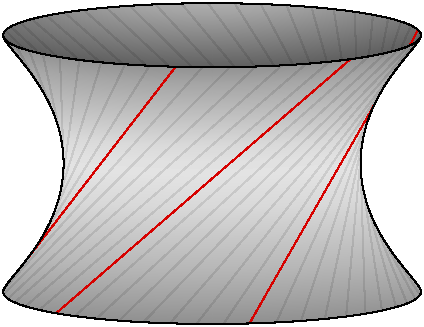
\includegraphics[height=2in]{main/Fig15-2-SinglyRuledHyperboloid-good}
\caption{Any three skew lines in space lie on a unique 
(and necessarily 
smooth) quadric surface, and all belong to the same 
ruling.
\index{ruling}%
}
\label{Fig15.2}
\end{figure}

\begin{enumerate}
\item Prove that $C$ lies on a unique quadric, and that $H^2(\sI_C) = 0$.
\index{quadric surface!containing three given lines}%
\item Compute the 
Hartshorne--Rao module
 $D(C)$.
\index{Hartshorne--Rao module}%
\item Show that if $\Gamma$ is the union of 3 points in $\PP^3$ then
$H^1\sI(\Gamma) = 0$ if and only~if the three points are collinear.
\item Using the exact sequence in cohomology coming from the short
exact sequence
$$
0\to \sI_C \ruto {\ \ell} \sI_C(1) \to \sI_\Gamma(1) \to 0 ,
$$
where $\ell$ is a linear form, show that the map of vector spaces
$$
H^1(\sI_C) \ruto {\ \ell} H^1(\sI_C(1))
$$
has rank $<2$ if and only~if $\ell$ vanishes on 3 collinear points on the
three lines (including the case when $\ell$ vanishes identically on one
of the lines).
Conclude that if a different union $C'$ of 3 skew lines is linked to $C$,
then $C'$ lies on the same quadric as $C$.
\end{enumerate}
See \cite{Migliore} for more examples of this type.
\end{exercise}

\begin{exercise}
Compute the 
Hilbert function
\index{Hilbert function}%
of the 
Hartshorne--Rao module
\index{Hartshorne--Rao module}%
 of a curve
of type $(a,b)$ on a smooth quadric surface.

Hint: The ideal sheaf of the curve on the quadric $Q$ is an extension
of the ideal sheaf of the quadric in $\PP^3$
with the ideal sheaf of the curve on the quadric, which is
$$
\sO_Q(-a,-b) = \pi_1^*(\sO_{\PP^1}(-a)) \otimes \pi_2^*(\sO_{\PP^1}(-b)),
$$
where $\pi_1, \pi_2$ are the projections to $\PP^1` `$. Use the
\index{K\"unneth formula}%
K\"unneth formula
$$
H^1(\sO_Q(p,q)) = H^1(\sO_{\PP^1}(p)) \otimes H^0(\sO_{\PP^1}(q)) \oplus
H^0(\sO_{\PP^1}(p)) \otimes H^1(\sO_{\PP^1}(q))
$$
to compute the necessary cohomology.
\end{exercise}

\begin{exercise}[linkage addition \cite{Schwartau}]
\label{Liaison addition}
Suppose that $I, J$ are saturated ideals defining purely 1-dimensional
\index{linkage addition}%
subschemes of $\PP^3$
and that $f,g$ is a regular sequence with $f\in I$ and $g\in J$.
Prove that $g I \cap fJ = (fg)$, and conclude that if $I,J$ are saturated
codimension 2 ideals
defining purely 1-dimensional schemes $C,C'$ in $\PP^3$
then $(gI+fJ)$ is a saturated ideal defining a purely 1-dimensional
scheme $C''$ with $D(C'') = D(C)(-\!\deg g) \oplus D(C')(-\!\deg f)$.

Hint: Use the exact sequence
$$
0\to (fg) \to gI \oplus fJ \to gI+fJ \to 0
$$
and the corresponding exact sequence of quotients by these ideals.
\end{exercise}


\begin{exercise}[basic double links]\label{Basic double links}
The special case of the construction in Exercise~\ref{Liaison addition}
\index{double links}%
in which $C'$ is trivial is already interesting.

\begin{enumerate}
\item Show that if $I$ is a 
saturated ideal of codimension 2
\index{saturated ideal!of codimension 2}%
defining a purely 1-dimensional scheme $C$ in $\PP^3$
and $(f, g)$ is a regular sequence with $g\in I$,
then $fI+(g)$ defines a scheme $C'$ with $D(C') = D(C)(-\!\deg f)$.

\item Show directly that, with notation as above, $C'$ is directly
linked to $C$
in two steps. Since the degrees of the generators of $D(C')$ are more
positive, this
is sometimes called an \emph{ascending double link}. Geometrically it
\index{double link!ascending}%
amounts to taking the
union of $C$ with some	components that are 
complete intersections.
\index{complete intersections}%
\end{enumerate}
\end{exercise}

\begin{exercise}~\label{adjointness}
Here is a more general form of the last step in the proof of 
Proposition~\ref{similarities}(1). 
Suppose that $B\to A$ is a homomorphism
of rings, $X$ is an $A$-module and $Y$ is a
$B$-module. Show that there is a natural transformation
$$
\phi: \Hom_A(X, \Hom_B(A, Y)) \cong \Hom_B(X,Y)
$$
and that if $X = \Hom_B(A,Y)$, then the map
$$
A\to \Hom_A(\Hom_B(A,Y), \Hom_B(A, Y))
$$
taking an element $a\in A$ to multiplication by $a$ on the $A$-module
$\Hom_B(A, Y)$
is sent by $\phi$ to the evaluation map $\alpha \mapsto \alpha(a)$ for
$\alpha \in \Hom_B(A,Y)$.
\end{exercise}

\subsection*{Ropes and ribbons}
The simplest way to construct well-behaved nonreduced curves is
to take neighborhoods of smooth ones. Ropes and ribbons are examples of
this sort:


\begin{definition}
The \emph{rope defined from a curve $C \subset \PP^n$} is the scheme
$V(I^2_C)$ defined by the square of the ideal $C$.
\index{rope}%
\unif
\end{definition}

\begin{exercise}\label{hilbert function of rope}
If $C$ is the rope defined from a line $L\subset \PP^3$ then the Hilbert
function $h_C(m)$ and Hilbert polynomial $p_C(m)$ are both equal to
$3m+1$. Thus $C$ has degree 3 and
arithmetic genus 0. Note that the degree can also be computed as the
degree of
a general hyperplane section, since this is defined by the square of
the ideal of a point
in $\PP^2` `$.

Hint: Count the monomials of each degree in square of the ideal of a line.
\end{exercise}

\begin{exercise} To see why the rope in Exercise~\ref{hilbert function
of rope} should look like a twisted cubic, show that it is the flat
limit of a twisted cubic as follows:
Let $X \subset \PP^3$ be the twisted cubic with parametrization $x_i =
s^it^{3-i}$. Consider the one-parameter subgroup of $\PGL_4$ given in
homogeneous coordinates $x_0,\dots, x_3$ on $\PP^3$ by
$$
A_t : (x_0,\dots,x_3) \mapsto (tX_0, X_1, X_2,tX_3).
$$
Show that the 
flat limit,
\index{flat limit}%
 as $t\to 0$, of the 
\index{twisted cubics}%
twisted cubics
 $A_t(C)$
is the rope $V(X_0^2, X_0X_1,X_1^2)$.

Hint: Use the description of $I(X)$ as the ideal of $2\times 2$ minors of
$$
\begin{pmatrix}
x_0 &x_1&x_2\\
x_1& x_2& x_3
\end{pmatrix}
.
$$
\end{exercise}


\begin{exercise}\label{line and rope}
We saw in Section~\ref{LinkageIntro} that a twisted cubic curve is linked
to a line by the 
complete intersection of two quadrics.
\index{complete intersection!of two quadrics}%
Show that the same is true for the rope of
Exercise~\ref{hilbert function of rope}.
\end{exercise}

If $C$ is the rope defined from a line in $\PP^2` `$, then the Zariski
tangent space to $C$ at
any point is 2-dimensional; that is, it looks like a ribbon. More
generally:

\begin{definition}
By a \emph{ribbon} $X \subset \PP^n$ we mean a scheme of pure dimension~1
\index{ribbon}%
and multiplicity 2 whose support is a smooth, irreducible curve $C \subset
\PP^n$ and whose 
Zariski tangent space
\index{Zariski tangent space}%
 at every point is 2-dimensional
(Figure~\ref{Fig15.3}).
\begin{figure}
\vskip-5pt
\centerline {\includegraphics[width=2.4in]{"main/Fig15-3"}}
\vskip-8pt
\caption{A ribbon supported on a line.}
\label{Fig15.3}
\end{figure}
\end{definition}

\begin{exercise}
Suppose that $C\subset \PP^n$ is a ribbon. Show that $C$ is
contained in the rope defined from $C_{\mathrm{red}}$, and show that
the degree of $C$ is twice 
that
of $C_{\mathrm{red}}$.

Hint: Look at hyperplane sections of $C$.
\end{exercise}

Unlike ropes, there are many different ribbons $C$ with the same smooth
curve $C_{\mathrm{red}}$,
and they can have different 
arithmetic genera.
\index{arithmetic genus}%
Suppose that $C\subset \PP^3$ is a ribbon such that $X = C_{\mathrm{red}}$
is the line $V(x_0,x_1)$.
Since $C$ is contained in the rope defined from $X$ we must have
$(x_0^2, x_0x_1,x_1^2) \subset I(C)$. The tangent space to $C$ at a
point $(0,0,s,t)$ meets the line $X' = V(x_2, x_3)$
at some point $(F(s,t),G(s,t),0,0)$, so $F$ and $G$ define a morphism
$\PP^1 \to \PP^1$;
thus they are homogeneous polynomials of the same degree $d$. It follows
that $I(C)$ also contains the element
$x_0 G(x_2, x_3) - x_1F(x_2,x_3)$. Show that the ideal of $C$ is obtained
by adding this form to the ideal of the rope, that is,
$$
I_C \; = \; \big(X_0^2, X_0X_1, X_1^2, F(X_3,X_4)X_0 + G(X_3,X_4)X_1\big)
.
$$
In case $d=1$, show that $C$ lies on a smooth quadric.

\subsection*{
General adjunction
}

The next two exercises illustrate Theorem~\ref{general adjunction}:

\begin{exercise}\label{codimension0}
Show that if $C\to D$ is a map of smooth curves with 
ramification index
\index{ramification index}%
\index{general adjunction}%
$e$ at $p\in C$, and $t$ is a local
analytic parameter at $p$, then
locally analytically at $p$ the sheaf $\sHom_C(\sO_C, \omega_D)$
is $\sO_C(e)$.
\end{exercise}

\begin{exercise}\label{codimension1}
Show that if $C\subset S$ is a
Cartier divisor
\index{Cartier divisor}%
on a surface $S$ with canonical sheaf $\omega_S$,
then $\sExt^1(\sO_C, \omega_S) \cong \sO_C\otimes \sO_S(C)$, and thus
$$K_C = (K_S+C)\cap C.$$
\index{linkage|)}%
\end{exercise}


%footer for separate chapter files

\ifx\whole\undefined
\makeatletter\def\@biblabel#1{#1]}\makeatother
\gdef\urlhook{\url}
\bibliography{slag}
\bibliographystyle{msribib}


%%%% EXPLANATIONS:

% f and n
% some authors have all works collected at the end

\catcode`\^\active
%if ^ is followed by 
% 1:  print f, gobble the following ^ and the next character
% 0:  print n, gobble the following ^
% any other letter: print letter
\makeatletter
\def^#1{\ifx1#1f\expandafter\@gobbletwo\else
        \ifx0#1n\expandafter\expandafter\expandafter\@gobble\else#1\fi\fi}
\makeatother
\let\moreadhoc\relax
\def\indexintro{%An author's cited works appear at the end of the
%author's entry; for conventions
%see the List of Citations on page~\pageref{loc}.  
%\smallbreak\noindent
The letter `f' after a page number indicates a figure, `n' a footnote.}
\printindex[gen]
%requires makeindex
\end{document}
\else
\fi




%header and footer for separate chapter files

\ifx\whole\undefined
\documentclass[12pt, leqno]{book}
\usepackage{graphicx}
\usepackage{eps-to-pdf}
\input style-for-curves.sty
%\input sl-macros.sty
\usepackage{hyperref}
\usepackage{showkeys} %This shows the labels.
\usepackage{msribib}
\usepackage{pdfpages}
\usepackage{draftwatermark}
\SetWatermarkText{DRAFT:\ \today}
\SetWatermarkScale{2}
\SetWatermarkColor[gray]{0.9}

%\usepackage{SLAG,msribib,local}
%\usepackage{amsmath,amscd,amsthm,amssymb,amsxtra,latexsym,epsfig,epic,graphics}
%\usepackage[matrix,arrow,curve]{xy}
%\usepackage{graphicx}
%\usepackage{diagrams}
%
%%\usepackage{amsrefs}
%%%%%%%%%%%%%%%%%%%%%%%%%%%%%%%%%%%%%%%%%%
%%\textwidth16cm
%%\textheight20cm
%%\topmargin-2cm
%\oddsidemargin.8cm
%\evensidemargin1cm
%
%%%%%%Definitions
%\input preamble.tex
%\input style-for-curves.sty
%\def\TU{{\bf U}}
%\def\AA{{\mathbb A}}
%\def\BB{{\mathbb B}}
%\def\CC{{\mathbb C}}
%\def\QQ{{\mathbb Q}}
%\def\RR{{\mathbb R}}
%\def\facet{{\bf facet}}
%\def\image{{\rm image}}
%\def\cE{{\cal E}}
%\def\cF{{\cal F}}
%\def\cG{{\cal G}}
%\def\cH{{\cal H}}
%\def\cHom{{{\cal H}om}}
%\def\h{{\rm h}}
% \def\bs{{Boij-S\"oderberg{} }}
%
%\makeatletter
%\def\Ddots{\mathinner{\mkern1mu\raise\p@
%\vbox{\kern7\p@\hbox{.}}\mkern2mu
%\raise4\p@\hbox{.}\mkern2mu\raise7\p@\hbox{.}\mkern1mu}}
%\makeatother

%%
%\pagestyle{myheadings}

%\input style-for-curves.tex
%\documentclass{cambridge7A}
%\usepackage{hatcher_revised} 
%\usepackage{3264}
   
\errorcontextlines=1000
%\usepackage{makeidx}
\let\see\relax
\usepackage{makeidx}
\makeindex
% \index{word} in the doc; \index{variety!algebraic} gives variety, algebraic
% PUT a % after each \index{***}

\overfullrule=5pt
\catcode`\@\active
\def@{\mskip1.5mu} %produce a small space in math with an @

\title{A Chapter from ``The Practice of Algebraic Curves"}
\author{\copyright David Eisenbud and Joe Harris}
%%\includeonly{%
%0-intro,01-ChowRingDogma,02-FirstExamples,03-Grassmannians,04-GeneralGrassmannians
%,05-VectorBundlesAndChernClasses,06-LinesOnHypersurfaces,07-SingularElementsOfLinearSeries,
%08-ParameterSpaces,
%bib
%}

\date{\today}
%%\date{}
%\title{Curves}
%%{\normalsize ***Preliminary Version***}} 
%\author{David Eisenbud and Joe Harris }
%
%\begin{document}

\begin{document}
\maketitle

\pagenumbering{roman}
\setcounter{page}{5}
%\begin{5}
%\end{5}
\pagenumbering{arabic}
\tableofcontents
\fi


\chapter{Scrolls and the curves they contain}
\label{ScrollsChapter}

If you've never read T. S. Eliot's {\it Old Possum's Book of Practical Cats}, 
you could do worse than start with ``The naming of cats'',
where the poet tells us that
\begin{quote}%
The Naming of Cats is a difficult matter [\dots]\\
a cat must have THREE DIFFERENT NAMES
\end{quote}%

\noindent %leave blank line above so the skips above and below quote match
\emdash one for daily use, one complex and unique, and one ineffable.
So it is with the class of varieties
\index{Eliot, Thomas Stearns}%
\index{rational normal scroll}%
\index{scroll}%
known as \emph{rational normal scrolls}. Although they're some of the
\index{scroll|(}%
\index{rational normal scroll|see scroll}%
simplest subvarieties in projective space\emdash the first examples
are shown in Figure~\ref{Fig16.1}\emdash they have a deeper aspect and
myriad applications (for instance, in describing the embeddings of
curves of low degree and genus), and can be examined from three rather
different points of view, each useful in a different context. We
%
\begin{figure}[h]
\includegraphics[height=1.1in]{"main/Fig16-1A"}\qquad
\includegraphics[height=1.1in]{"main/Fig16-1B"}\qquad
\includegraphics[height=1.1in]{"main/Fig16-1C"}\qquad
\includegraphics[height=1.1in]{"main/Fig16-1D"}%
\caption{The smallest scrolls: from the left, $S(0,1) \cong \PP^{2}$;
$S(0,2)$, the cone over a conic; $S(1,1)\subset \PP^{3}$ the union of
lines joining corresponding points of two skew lines, isomorphic to a
smooth quadric; and $S(1,2)\subset \PP^{4}$ the union of the lines
joining corresponding points on a line and a conic.
\vspace*{-10pt}
}
\label{Fig16.1}
\end{figure}
%
will take up each in turn.%
\footnote{However, we claim no secret knowledge comparable to the
feline name ``that no human research can discover-- But THE CAT
HIMSELF KNOWS.'' The full text of Eliot's poem is available at
https://poets.org/\allowbreak poem/naming-cats.%
}%

{\it In this chapter 
we will refer to rational normal scrolls simply as scrolls.}
We first give
a classical geometric construction, then an algebraic description that
allows one to ``find'' the scrolls containing a given variety, and
then a more modern geometric definition that makes it easy to
understand the divisors on a scroll. Finally, we turn to some of the
applications to the embeddings of curves. We will focus on the case of
2-dimensional scrolls because this is the 
one
that occurs most often in our applications.

\section{Some classical geometry}\label{daily name}

To construct a scroll of dimension 2 in $\PP^r` `$, we start by choosing
integers 
$a_1\ge\nobreak0$
and  
$a_2\ge1$
with $a_1 + a_2 = r-1$, and
consider  a pair of complementary linear subspaces $\PP^{a_1}$ and
$\PP^{a_2} \subset \PP^r = \PP(V)$\emdash that is, we express an
$(r+1)$-dimensional vector space $V$ as a direct sum $V =  V_1 \oplus
V_2$ of subspaces $V_1, V_2 \subset V$ of dimensions $a_1+1$ and
$a_2+1$. For simplicity we will always assume, without loss of 
generality, that $a_{1}\leq a_{2}$.

Next, for $i`=`1,2$, we take $\phi_i \!:\!  % avoid very underfull line
\PP^1 `\to` \PP^{a_i}$ to be the
parametrization of the rational normal curve of degree $a_i$ given by
a basis of homogeneous polynom\-ials of degree $a_i$ (if $a_i = 0$ this
is just the constant map from $\PP^1$ to a point). Finally, we define
the scroll $S(a_1, a_2)$ to be the union of the lines
\label{thescroll}
$$
S(a_1,a_2)\colonequals\bigcup_{p\in \PP^1} \overline{\phi_1(p)\, \phi_2(p)}.
\vspace*{-2pt}
$$
We call the curve $C_{a_{1}}$ a \emph{directrix} of the scroll; if $a_{1}<a_{2}$ this
is unique. 
\index{directrix}%
The family of lines
$ \overline{\phi_1(p) \phi_2(p)}$ is called a 
\index{ruling}%
\emph{ruling} of the scroll, and this is unique except when $a_{2} = 1$,
the case of $S(0,1) = \PP^{2}$, and the case of a smooth quadric surface in $ S(1,1)\subset \PP^{3}$.

In the degenerate case $a_{1}= 0$, the surface $S(0,a_{2})$ is the cone
in $\PP^{a_{2}+1}$ over a rational normal curve of degree $a_{2}$.
 Since $S(0,a_2)$ is singular when $a_2\geq 2$,
it is useful to consider the surface
$$
\tilde S(0, a_2) \colonequals  \bigl\{@ (t, q) \in \PP^1 \times \PP^r
\mid q \in \overline{\phi_1(t), \phi_2(t)}@\bigr\}.
$$
This is the 
\index{blow-up!of a cone}%
blow-up of the cone $S(0, a_2)$ at its vertex; like the
surfaces $S(a_1,a_2)$ with $a_1 > 0$ it is a $\PP^1$ bundle over $\PP^1$
and thus is smooth. As we shall see, $\tilde S(0, a_2)$ is isomorphic
to the scroll $S(1, a_2+1)$.
It is not hard to prove directly that $S(a_1,a_2)$ is an algebraic
variety, and we shall soon write down its defining equations.

From the description above we can immediately deduce the dimension and
degree of a scroll:

\begin{proposition}
\begin{enumerate}
\item $S(a_1,a_2)$ is a nondegenerate surface.
\item $S(a_1,a_2)$ has degree $a_1+a_2$, and codimension $a_1+a_2-1$.
\item $S(a_{1},a_{2})$ is nonsingular if $a_{1}>0$.
\unif
\end{enumerate}
\end{proposition}

\begin{proof}
The rational normal curves separately span the spaces $\PP^{a_i}$, so a
hyperplane containing both of them would contain $\overline{\PP^{a_1},
\PP^{a_{2}}} = \PP^r` `$, proving nondegeneracy.

It is clear from our description that $S$ is 2-dimensional, and thus of
codimension $a_{1}+a_{2}+1 -2 = a_{1}+a_{2}-1$.

To compute the degree, we choose a general hyperplane $H$ containing
$\PP^{a_{1}}$. The intersection $H\cap C_{2}$ consists of $a_{2}$
reduced points. Thus the intersection $H\cap S$ consists of $C_{1}$
and the $a_{2}$ reduced lines connecting
the points of $H\cap C_{2}$ with their corresponding points on $C_{1}$;
this union has degree $a_{1}+a_{2}$.

If $0< a_{1}$ we also see from this argument that, given any point  $p\in
S(a_{1},a_{2})$, there is
a hyperplane section that is nonsingular at $p$, and thus $S(a_{1},a_{2})$
is nonsingular at $p$.
\end{proof}

A completely parallel construction creates 
scrolls of
any dimension $s$. Start with a series of integers $0 \leq a_1 \leq
\dots \leq a_s$;
set $r + 1 = \sum_{i=1}^{s}(a_{i}+1)$,  and
decompose $\CC^{r+1}$ as
$$
\CC^{r+1} = \bigoplus_{i=1}^{s}\CC^{a_{i}+1}.
$$
Let $\PP^{a_{i}}\subset \PP^{r}$ be the subspaces corresponding to the
summands,  choose for each~$i$ a
map $\phi_i : \PP^1 \to \PP^{a_{i}}$  given by a basis of homogeneous
polynomials of degree $a_i$, and define the scroll $S \subset \PP^{r}$ by
$$
S=S(a_{1}, \dots, a_{s}) \colonequals  \bigcup_{p\in
\PP^{1}}\overline{\phi_1(p), \phi_{2}(p), \dots, \phi_{s}(p)}.
$$
For example, $S(a_{1})$ is the rational normal curve of degree $a_{1}$. In
general, the variety $S$ is nondegenerate of codimension $r-s$ and degree
$\sum a_{i} = r-s+1$. The proof is similar to the one we gave for $s=2$.

To put this construction in context, we recall that by
Corollary~\ref{minimal degree bound}
Any irreducible, nondegenerate variety $X$ of codimension $c$ in
$\PP^{r}$ has degree $\geq c +1$.

Thus scrolls are \emph{varieties of minimal degree}. The reader already
\index{minimal degree}%
knows that the rational normal curves of degree $a$ in $\PP^{a}$ are the
only irreducible, nondegenerate curves of degree $a$ and codimension
$a-1$. A celebrated theorem of del Pezzo (for surfaces) and Bertini
\index{del Pezzo, Pasquale}%
\index{Bertini, Eugenio}%
(in general) generalizes this statement;
a proof may be found in \cite{Eisenbud-Harris-Centennial}.

\begin{theorem}\label{classification of scrolls}
An
irreducible, nondegenerate variety $X\subset \PP^{r}$  
satisfying
$@\deg X `=
\codim X+1$ is either a 
scroll, a quadric hypersurface,
the Veronese surface in $\PP^{5}$ or a cone over the Veronese surface.
\qed
\end{theorem}

One interesting way to view the construction of a scroll is that we chose
subvarieties $C_{i}\subset \PP^{a_{i}}$ and a one-to-one correspondence
between them, that is, a subscheme
$\Gamma\subset \prod C_{i}$ that projects isomorphically onto each
$C_{i}$; the scroll is then the
union of the planes spanned by sets of points $p_{i}\in C_{i}$ that
are ``in correspondence''. There are other interesting varieties
constructed starting with other choices of subvarieties $C_{i}$ and
subschemes\emdash not necessarily reduced\emdash of $\prod C_{i}$. See
\index{Sammartano, Alessio}%
\cite{Eisenbud-Sammartano} for an exploration of this idea.

Despite the choices made in the definition 
on page~\pageref{thescroll}, we're entitled to talk about
{\it the\/} scroll $S(a_1,\dots,a_s)$:

\begin{proposition}\label{uniqueness of scrolls}
Up to a linear automorphism of the ambient projective space $\PP$, 
the scroll $S(a_1,\dots,a_s)$ is independent of the choices made in its
definition.
\unif
\end{proposition}

\begin{proof}
In the construction of
$S(a_{1},\dots,a_{s})$ we chose
\begin{enumerate}
\item independent subspaces $\PP^{a_i}\subset \PP$,
\item a rational normal curve in each subspace, and
\item an isomorphism between these curves.
\end{enumerate}
Elementary linear algebra shows that there are automorphisms of $\PP$
carrying any choice of linearly independent subspaces to any other choice. Further,
since the rational normal curve of degree $a$ is unique up to an
automorphism of $\PP^{a}$, the two choices in (2) differ by a linear
automorphism. Finally, any automorphism of $C_{a_{i}}\cong \PP^{1}$
extends to an automorphism of $\PP^{a_{i}} = |\cO_{\PP^{1}}(a_{i})|$, and
this extends to an automorphism of $\PP$ fixing all the 
$\PP^{a_{j}}$, for $j\neq i$ pointwise,
showing that $S(a_{1},\dots, a_{s})$ is independent, up to an automorphism of
the ambient space, of the choice in (3)  as well.
\end{proof}

\section{1-generic matrices and the equations of scrolls}\label{particular
name}

Suppose that a scheme $X $ is embedded in $\PP^r$ by a 
\index{1-generic matrix}%
\blue{complete linear series,}
\index{complete linear series}%
and that
$\sO_X(1)$ can be ``factored'' as a tensor product $\sL\otimes
\sM$ of invertible sheaves on $X$. If we pick bases of $p$  elements
$\{\ell_i\}\subset H^0(\sL)$ and  $q$  elements $\{m_i\} \subset H^0(\sM)$
then the multiplication map
\index{multiplication map}%
$$
\mu: H^0(\sL) \otimes H^0(\sM) \to H^0(\sO_{X}(1))= H^0(\sO_{\PP^r}(1))
$$
gives rise to
a $p\times q$ matrix $M_\mu$ of linear forms on $\PP^r$ whose $i,j$
entry is $\mu(\ell_im_j)$.
More abstractly, this is a linear space of matrices obtained from the
``adjunction'' isomorphism
$\Hom(A\otimes B, C)\cong \Hom(A, \Hom(B,C))$.

Regarding the sections of invertible sheaves as rational functions on $X$,
we see from the commutativity of
multiplication that the $2\times 2$ minors
of
\vspace*{3pt}
$$
\vspace*{3pt}
\det \begin{pmatrix}
\ell_{i_1}m_{j_1} & \ell_{i_1}m_{j_2}\\
\ell_{i_2}m_{j_1} &\ell_{i_2}m_{j_2}
\end{pmatrix},
$$
vanish on $X$\emdash that is, the ideal of $2\times 2$ minors $I_2(M_\mu)$
is contained in the homogeneous ideal
of $X$. We will show that the ideal of a scroll is
generated by such minors.

\begin{example}
We have already seen this phenomenon in the case of the rational normal
curve $C_a\subset \PP^a$ if $X = \PP^1` `$.
Here $C_{a}$ is embedded by the complete
linear series $|\sO_{\PP^1}(a)|$, and  we can write $\sO_{\PP^1}(a) =
\sO_{\PP^1}(1)\otimes \sO_{\PP^1}(a-1)$.
If we take bases $s^it^j$ in each of $H^0(\cO_{\PP^1}(1))$,
$H^0(\cO_{\PP^1}(a-1))$ and $H^0(\cO_{\PP^1}(a))$
we get
the $2\times a$ matrix
$$
M_\mu \colonequals
\begin{pmatrix}
x_0&x_1&\dots&x_{a-1}\\
x_1&\dots&x_{a-1}&x_a
\end{pmatrix}.
$$
When restricted to $\PP^1` `$, this becomes
$$
M_a = \bordermatrix{
& s^{a-1}&s^{a-2}t&\dots&t^{a-1}\cr
s&  s^{a}& s^{a-1}t&\dots&st^{a-1}\cr
t&  s^{a-1}t& s^{a-2}t^{2}&\dots&t^{a}\cr
}$$
where we have written $s,t$ for the basis of $H^0(\sO_{\PP^1}(1))$,
and bordered the matrix
with the corresponding bases of $H^0(\sO_{\PP^1}(1))$ and
$H^0(\sO_{\PP^1}(a-1))$, and it is obvious
that the minors of $M_a$ are 0.
\end{example}

By a \emph{generalized row} of $M_{a}$ we mean a $\CC$-linear combination
\index{generalized row}%
of the given rows of $M_{a}$. Note that the points at which the $2\times2$ 
minors of $M_{a}$ vanish are the points at which the evaluations of
the two rows are linearly dependent; that is, the points at which some
generalized row of $M_{a}$ vanishes identically.

\begin{definition}
A matrix of linear forms $M$ is  \emph{$1$-generic} if every generalized
row of $M$
consists of $\CC$-linearly independent forms.
\index{1-generic}%
\end{definition}

\begin{proposition}\label{some generators}\label{some equations}
Let $X$ be
an irreducible, reduced variety. If $\sL,\sM$ are invertible
sheaves on $X$
then
the matrix $M_\mu$ coming from the map $\mu:H^0(\sL) \otimes H^0(\sM)
\to H^0(\sL\otimes \sM)$
is $1$-generic.
\unif
\end{proposition}

\begin{proof} The entries of the generalized row of $M_\mu$ corresponding
to $s\in H^0(\sL)$
are a basis of $s\cdot H^0(\sM) \cong H^0(\sM)$, and are thus
linearly independent.
\end{proof}

\begin{example}
For example, the matrix
$$
M = \Bigl(\,\begin{matrix}
x &y\\[-2pt]
z&x
\end{matrix}\,
\Bigr)
$$
over $\CC[x,y,z]$ is  1-generic, since if a row and column transformation
produced a 0 the determinant would be a product of linear forms, while
$\det M = x^2-yz$ is irreducible. ($M$ corresponds to the
multiplication
$H^{0}(\sO_{\PP^{1}}(1)) \otimes
H^{0}(\sO_{\PP^{1}}(1))
\to H^{0}(\sO_{\PP^{1}}(2)).
$)

On the other hand, the matrix
$$
M' = \Bigl(@\begin{matrix}
x &y\\[-2pt]
-y&x
\end{matrix}\,\Bigr)
$$
over $\CC[x,y]$ is not 1-generic, since
$$
\Bigl(\,
\begin{matrix}
1&0\\[-2pt]
\!-i&1
\end{matrix}
\,\Bigr)
\,
M'
\,
\Bigl(\,
\begin{matrix}
1&0\\[-2pt]
i&1
\end{matrix}
\,\Bigr)
=
\Bigl(\,
\begin{matrix}
x+iy&0\\[-2pt]
0&x-iy
\end{matrix}
\,\Bigr)
.
$$
The matrix $M'$ would be 1-generic if we restricted scalars to
$\RR$; thus the definition depends on the field.
\end{example}

\begin{lemma}\label{existence of 1-generic}\label{variables needed}
\label{size of 1-generic} There exist $1$-generic $p\times q$ matrices of
linear forms in $r+1$ variables over $\CC$ if and only~if $r\geq p+q$.

If $M$ is 1-generic and involves more than $p+q-1$ variables, then the
restriction of $M$ to a general hyperplane is still $1$-generic.
\unif
\end{lemma}

\begin{proof} Consider a map of vector spaces $\mu : A\otimes B \to C$,
where we regard $C$ as a
space of linear forms.
With notation as above, if $\ell_i\otimes m_j\in \ker \mu$, then the $i,j$
entry of $M_\mu$ is 0 and similarly for
any \emph{pure} tensor $\ell\otimes m\in A\otimes B$. Thus $M_\mu$
is 1-generic if and only~if the linear subspace
$\ker \mu \subset  A\otimes B$
is disjoint from the set of pure tensors. Under the isomorphism $A\otimes
B \cong \Hom (A^*, B)$
the set of pure tensors corresponds to matrices of rank 1, and this set
has codimension $(p-1)(q-1) = pq-p-q+1$
in $\Hom(A^*, B)$. 
(Proof:
a rank 1 matrix corresponds to the choice of
a 1-quotient of $A^*$ and a 1-dimensional subspace
of $B$, thus a point in $\PP^q \times \PP^p$.)
Thus
for $\mu$ to correspond to a  1-generic matrix,  we must have $\codim
\ker \mu \geq q+p-1$. Since $\codim \ker \mu = \dim \im \mu\subset C$
we see that any 1-generic matrix must involve at least $q+p+1$ variables.

Furthermore, the restriction of $M_\mu$ to a hyperplane corresponds to
the composite homomorphism
$A\otimes B \to C \to C/\langle x \rangle$, or equivalently to the
addition of one element to $\ker \mu$, and thus
if $M_\mu$ is 1-generic and involves $>q+p-1$ variables, then the
restriction to a general hyperplane
is again 1-generic.
\end{proof}

We will see that 1-generic $2\times r$ matrices correspond to scrolls. The
beginning of the story is the
calculation of the codimension of the ideal $I_2(M)$ generated by the
$2\times 2$ minors of $M$:

\begin{lemma}\label{codim of 2,n 1-generic}
If $M$ is a $1$-generic $2\times b$ matrix of linear forms in
$\CC[x_0,\dots, x_r]$ then
$V(I_2(M))$ is irreducible of codimension $b-1$.
\unif
\end{lemma}

\begin{proof}
The algebraic set $V \colonequals   V(I_2(M))$ is the set of points
on which a generalized row $\rho_\lambda, \ \lambda\in \PP^1$ of $M$
vanishes. Thus the map
$$
W \colonequals  \{(p, \lambda) \in \PP^{r}\times \PP^{1}\mid p\in
V(\rho_{\lambda})\} \to V
$$
is surjective. All the fibers of the second projection $\pi_{2}: W\to
\PP^{1}$ are isomorphic to $\PP^{r-b}$, so $W$ is
irreducible of dimension $r-b+1$, and thus $V$ is irreducible. Each
fiber $\pi_{2}^{-1}(\lambda)$
injects into $V` `$, and the images of these fibers are distinct since
otherwise the entries of $M$ would all
be contained in a single generalized row, contradicting
Lemma~\ref{variables needed}. It follows
that $V$ also has dimension $r-b+1$, as required.
\end{proof}

We have seen in Proposition~\ref{RNC generators} that the ideal of
minors of
$$
M_{a}\colonequals
\begin{pmatrix}
x_0&x_1&\dots&x_{a-1}\\
x_1&x_2&\dots&x_{a}\\
\end{pmatrix}
$$
generates the ideal of the rational normal curve of degree $a$ in $\PP^a`
`$, and is thus prime. More generally:

\begin{theorem}\label{1-generic basics}
Let $I = I_2(M)$  be the ideal generated by the $2\times 2$ minors of
a 1-generic, $2\times a$ matrix $M$
of linear forms in $S = \CC[x_0,\dots, x_n]$.
\begin{enumerate}

\item The ideal $I$ is prime, and $V(I)$ either is smooth, or is a cone
over a smooth variety.

\item If $a=r$ then $V(I)$ is a rational normal curve. More generally,
the variety $V = V(I) \subset \PP^r$ has degree $a$ and codimension $a-1$
and is thus a variety of minimal degree.
\unif
\end{enumerate}
\end{theorem}

\begin{proof}  By Lemma~\ref{codim of 2,n 1-generic},  $V(I)$ has
codimension $a-1$.
If the span of the linear forms in $M$ is not the whole space of linear
forms on $\PP^r` `$, then $V(I)$ is a cone,
so we may assume that the entries of $M$ generate the maximal ideal.

Let $p\in V(I)$ be a point, so that there is a generalized row of
$M$\emdash without loss of generality the second row\emdash whose
entries all vanish
at $p$. Since not all the linear forms
of $S$ can vanish at a point of $\PP^r` `$, we may make column
transformations to reduce to the case where
$\ell_{1,j}$ also vanishes at $p$ for all $j\neq 1$. Since the entries
of each generalized row are linearly independent, the ideal generated
by the entries of the second row define a plane of
$\Lambda$ codimension $a$ containing $p$.

Over the local ring $\sO_{\PP^r, p}$ the element $\ell_{1,1}$ becomes
a unit.
Thus, locally at $p$, the elements $m_{j}\colonequals  \ell_{2,j}+
\ell_{1,1}^{-1}\ell_{2,1}\ell_{1,j}$ for $j=2,\dots, a$ are in the
ideal generated
by the minors. Since the $\ell_{2,j}$ are independent regular parameters
in $\sO_{\PP^r, p}$ and
$\ell_{1,1}^{-1}\ell_{2,1}\ell_{1,j}$ is in the square of the maximal
ideal of $\sO_{\PP^r, p}$ the
$a-1$ elements $m_{j}$
are also regular parameters. Since $\codim I = a-1$, it follows that $I$
is prime and defines a smooth variety, as claimed.

If $a=r$ then $V(I)$ is a smooth, nondegenerate curve. In
Chapter~\ref{SyzygiesChapter} we will construct the Eagon--Northcott
complex $EN(M)$. By Theorem~\ref{ENgeneral}, the complex $EN(M)$ is a
free resolution,
and if $M'$ is the ideal of the rational normal curve, then $EN(M')$
is again a resolution. Since the Hilbert
function of $V(I)$ can be computed from the free resolution, it follows
that $V(I)$ has the same Hilbert function
as $V(I_2(M))$, and thus $V(I)$ is a rational normal curve.

If $a<r$ then by Lemma~\ref{some generators} there is linear form $\ell$
such that $M$ remains 1-generic modulo $\ell$.
Since $I_2(M)$ is prime it has the same degree and codimension as $I_2(M)
+(x)/(x) \subset S/(x)$, so by induction its degree
is $a$.
\end{proof}

We can use Theorem~\ref{1-generic basics} to prove a classic result of
Castelnuovo, characterizing large sets of
\index{Castelnuovo, Guido}%
points on a rational normal curve. It is a key element in
Theorem~\ref{Castelnuovo examples} below, which classifies
Castelnuovo curves of high
degree, 

\begin{corollary}[Castelnuovo's $2r+3$ lemma]
\label{Castelnuovo2r+3}
If\, $\Gamma\subset \PP^r$ is a set of $d \geq 2r+\nobreak 3$ distinct points in
\index{2@$2r+3$ lemma}%
\index{r@$2r+3$ lemma}%
linearly general position, then
$\Gamma$ is contained in a rational normal curve if and only~if $\Gamma$
imposes only $2r+1$
conditions on quadrics.
\end{corollary}
For a classical proof of Corollary~\ref{Castelnuovo2r+3} see for example
\cite[p.~531]{Griffiths-Harris1978}.

To understand the approach taken in the proof below, recall that in
the case of a twisted
cubic, whose equations are the minors of the matrix
$$
\begin{pmatrix}
x_0&x_1&x_2\\
x_1&x_2&x_3
\end{pmatrix}
$$
the first column defines a secant line to the twisted cubic, and the
two minors involving the first column are a regular sequence defining
the union of the twisted cubic and that secant line (see Figure~\ref{cubicAndLine}).
In general a rational normal curve may be defined by the 1-generic
matrix  associated to the product $H^0(\sO_{\PP^1}(1)) \otimes
H^0(\sO_{\PP^1}(r-1)) \to H^0(\sO_{\PP^1}(r))$,
and it follows from that description that the columns of the matrix
define the $(r-1)$-secant $(r-2)$-planes to the curve. In the proof
below we reconstruct the matrix starting from such a secant plane.

\begin{proof} Suppose first that $\Gamma$ is contained in a rational
normal curve $C$ of degree $r$ in $\PP^{r}$.
If $Q$ is a quadric vanishing on $\Gamma$ then by B\'ezout's theorem
$C\subset Q$. Since $C$ is arithmetically
Cohen--Macaulay, the dimension of the space of quadrics vanishing on
$C$ is
$$
\h^{0}(\sO_{\PP^{r}}(2)) - h^{0}(\sO_{C}(2r)) = \h^{0}(\sO_{\PP^{r}}(2))
-(2r+1)
$$
so $\Gamma$ imposes $2r+1$ conditions on quadrics.

Conversely, suppose that $\Gamma$ imposes only $2r+1$ conditions on
quadrics.
By Theorem~\ref{1-generic basics} it suffices to construct a 1-generic
$2\times r$ matrix $M$ whose minors vanish on
$\Gamma$. Note that the dimension of the space of quadrics on $\PP^r`
`$, which is $\tbinom{r+2}{2}$, is equal to the sum
$\tbinom{r}{2}+2r+1$, so the vector space of quadrics containing $\Gamma$
has dimension $\tbinom{r}{2}$.

Write $\Gamma = \{p_{1}, \dots, p_{d}\}$,
%Enumerate the points $p_i\in \Gamma$, 
and let $\Lambda = V(a_1,b_1)$
be the $(r-2)$-dimensional linear
space spanned by $p_1,\dots,p_{r-1}$.

The number of
conditions $\Lambda$ imposes on quadrics is $\tbinom{r}{2}$, but the $r-1$
points of $\Gamma \cap \Lambda$
already impose $r-1$ conditions, so the dimension of the space of quadrics
containing $\Lambda\cup \Gamma$
is $\tbinom{r}{2}-\bigl(\tbinom{r}{2}-(r-1)\bigr) = r-1.$ These quadrics
are contained in the ideal $(a_1,b_1)$, so a
basis for them
may be written as the $2\times 2$ minors that involve the first column
of a matrix
$$
M' \colonequals  \begin{pmatrix}
a_1&a_2&\dots&a_{r}\\
b_1&b_2&\dots&b_{r}
\end{pmatrix}.
$$
We will show first that $M'$ is 1-generic.

If $M'$ were not 1-generic then we could perform row and column operations
that do not change the
span of the first column or the span of the minors involving the first
column
to arrive at a matrix with an entry equal to 0. The minor
involving the first column and that column is nonzero, because the
quadrics defined by
these minors are linearly independent. But a reducible quadric can contain
only $2r$ linearly independent points, a contradiction proving that $M'$
is 1-generic.

It now suffices to show that all the minors of $M$ vanish at all the
points of $\Gamma$.
At a point in $p\in \Gamma$ that is not in $\Lambda$, at least one of
$a_1,b_1$ is nonzero.
Since each minor
of $M$ involving the first column vanishes at $p$, each pair
of scalars $(a_i(p),b_i(p))$ is a multiple of $(a_1(p), b_1(p))$. Thus
all the minors
of $M$ vanish at $p$, and thus vanish on at least $\geq 2r+3-(r-1) =
r+4$ points of $\Gamma$.

Because $a_2,\dots, a_r$ are linearly independent,
we may perform column operations to ensure that for $i=2, \dots, r$
the linear form
$a_i$ vanishes at all of $\{p_2,\dots, p_{r}\}$ except possibly at $p_i$.
Thus the minor of $M$ involving columns $i,j$ vanishes at each of
$p_2,\dots, p_r$ except possibly
$p_i,p_j$, thus at 
$r-3$ additional 
points, for a total of $2r+1$ points
of $\Gamma$. Since
$\Gamma$ imposes only $2r+1$ conditions on quadrics, the minors of $M$
vanish on all of $\Gamma$,
as required.
\end{proof}

The number $2r+3$ in Corollary~\ref{Castelnuovo2r+3} is sharp: if $C$
is a canonical curve of genus $r+2$ in $\PP^{r+1}$, then, since $C$
is arithmetically Cohen--Macaulay (Corollary~\ref{list of Castelnuovo curves}),
Corollary~\ref{ACM basics} implies that the points of a hyperplane
section lie on the same number of independent quadrics as does $C$,
and so,
by Corollary~\ref{canonical hilbert function} such points lie on the
same number of
quadrics as do $2r+2$ points on a rational normal curve.

\begin{fact}
In \cite{MR685427} a similar argument is used to show that if $\Gamma$
is a set of 
\redden{at least}
$2r+1+2d$ points in uniform position
imposing only
$2r+d$ conditions on quadrics, then $\Gamma$ lies on a rational normal
scroll of dimension $d$.
We do not know whether the requirement of 
\index{uniform position}%
uniform position can be weakened
to linearly general position,
as in the case $d=1$.
\end{fact}

\begin{corollary}\label{equations of scrolls} Let $a_{1}, \dots, a_{d}$
be nonnegative integers, and let
$$r = d-1+\sum_{i=1}^{d} a_{i}.$$
The ideal of $S(a_{1},\dots,a_{d})\subset \PP^{r}$ is generated by the
\index{minors!$2\times 2$}%
$2\times 2$ minors of the matrix
$$
\setcounter{MaxMatrixCols}{20}
\arraycolsep=3pt
M = \begin{pmatrix}
x_{1,0}&x_{1,1}&\dots&x_{1, a_{1}-1}&|&x_{2,0}&\dots&x_{2,
a_{2}-1}&|&\dots&|&x_{r,0}&\dots&x_{r, a_{r}-1}\\
x_{1,1}&x_{1,2}&\dots&x_{1, a_{1}}.  &|&x_{2,1}&\dots&x_{2,
a_{2}}&|&\dots&|&x_{r,1}&\dots&x_{r, a_{r}}
\end{pmatrix}
$$
Moreover, the scroll admits a linear projection to each $C_{a_i}$.
\unif
\end{corollary}

\begin{proof} We may think of the matrix $M$ as consisting of $d$
blocks, $M_{a_{i}}$. These blocks are 1-generic by Proposition~\ref{some
generators}. Since they involve distinct variables, it follows that $M$
is 1-generic. Thus by
Theorem~\ref{1-generic basics}, the ideal $I_{2}(M)$ is prime and of
codimension $d = \sum a_{i}-1$, as is the ideal of the scroll. Thus it
suffices to show that the minors of $M$ vanish on the scroll.

Let $C_{i}$ be the rational normal curve in the subspace
$\PP^{a_{i}}\subset\PP^{r}$.
As always, the set $V(M)$ is the union of the linear spaces on which
generalized rows of $M$ vanish; and each such space is the space spanned
by the points in the curves $C_{a_{i}}$ corresponding to the part of that
row in the block $M_{a_{i}}$\emdash that is, $V(I_{2}(M))$ is the union of
the spans of sets of corresponding points on the $C_{a_{i}}$, as required.
\end{proof}

In Theorem~\ref{matrix pencils} we will show that every
1-generic $2 \times (r-d)$ matrix of linear forms in $r$ variables can
be transformed by row and column transformations and a linear change
of variables to one of the type shown in
Corollary~\ref{equations of scrolls}, and thus the minors of any 1-generic
matrix define a scroll.

\section{Scrolls as images of projective bundles}\label{inscrutable name}

Recall that if $X$ is a scheme and $\sE$ is a locally free sheaf on
$X$ then $\PP(\sE) = \Proj(\Sym \sE)$ is a 
\emph{projective space bundle}, 
\index{projective space bundle}%
\index{space bundle}%
and comes equipped with a projection $\pi: \PP(\sE) \to X$
and a \emph{tautological invertible sheaf} $\sO_{\PP(\sE)}(1)$ that is
\index{tautological invertible sheaf}%
a quotient of $\pi^{*}(\sE)$ such that $\pi_{*}(\sO_{\PP(\sE)}(1)) =
\sE$, and thus with
$$
H^{0}(\sO_{\PP(\sE)}(1)) = H^{0}(\sE).
$$

Our third description of 2-dimensional scrolls is that they are the
images of projective space bundles
$$
\PP(\sO_{\PP^{1}}(a_{1})\oplus \sO_{\PP^{1}}(a_{2}))
$$
under the map given by the complete series associated to the 
\blue{tautological line bundle.}
\index{tautological line bundle}%
When both $a_{1}$ and $a_{2}$ are strictly positive,
we will see that this is an embedding, and in any case we will focus
on the projective bundle itself, which is always smooth. The case
of higher-dimensional scrolls is similar. We follow  
\cite[Chapter V]{Hartshorne1977}, but restrict
to the 2-dimensional rational case.

\begin{npt}
\begin{theorem}[{{\cite[Proposition V.2.2 and V.2.3]{Hartshorne1977}}}]
Suppose that $0\leq a_1\leq a_2$ are integers and let
$$
\sE = \sO_{\PP^1}(a_1) \oplus \sO_{\PP^1}(a_2).
$$
Let $X = \PP(\sE)$  be the corresponding $\PP^1$ bundle over $\PP^1$
and let $\pi: X \to \PP^1$ be the natural projection. Set $\sL =
\sO_{\PP(\sE)}(1)$, the tautological 1-quotient of $\pi^*(\sE)$.

The 
\blue{complete linear series} 
$|\sL|$ is basepoint free, and is very ample
\index{basepoint free}%
\index{very ample}%
\index{complete linear series}%
if $0<a_1$.
Let $\phi:X\to \PP^{a_1+a_2+1} = \PP^r$ be the corresponding morphism. The
image of $\phi$ is the scroll $S(a_1,a_2).$
More explicitly:
\begin{enumerate}
\item If $C_1, C_2\subset X$ are the curves defined by the projections
$\sE \to \sO_{\PP^1}(a_i)$, then $\phi(C_1)$ and 
$\phi(C_2)$
are defined by the vanishing
of the sections of $\sO_{\PP^1}(a_2)$ and  $\sO_{\PP^1}(a_1)$
respectively. Thus $C_i \cong \PP^1` `$,
and  the restriction of $\phi$ to $C_i$ embeds it in $\PP^{a_i}$ as the
rational normal curve of degree $a_i$.

\item The restriction of $\sL$ to the fiber $\PP^1$ of $\pi$ is
$\sO_{\PP^1}(1)$.

\item The fibers of $\pi$ meet each $C_i$ in a point. The images of $C_1,
C_2$ are contained in disjoint subspaces of $\PP^r` `$, and the fibers
of $\pi$ are mapped
to lines joining the corresponding points of the $C_i$.
\qed
\end{enumerate}
\end{theorem}

\begin{corollary}[{{\cite[Section V.2]{Hartshorne1977}}}]
Let $0\leq a_1\leq a_2$ be integers. The divisor class group of the
\index{divisor class group}%
scroll
$$
X\colonequals S(a_1,a_2) \subset \PP^r = \PP^{a_1+a_2+1}
$$
is generated by the class of the hyperplane section and the class
of a ruling. If $a_1 = 0$, then the blowup of $X$ at its singular point
is $S(1, a_2+1)\subset \PP^{r+2}$,
\medmuskip=3mu minus 2mu
\thickmuskip=4mu minus 2mu
and $C_1\subset S(1, a_2+1)$ is the exceptional divisor.  The 
\blue{blowup}
\index{blowup}%
map $S(1, a_2+1) \to S(0,a_2)$ corresponds to the isomorphism
$$
\PP(\sO_{\PP^1}(1) \oplus \sO_{\PP^1}(a_2+1)) \to \PP(\sO_{\PP^1}
\oplus \sO_{\PP^1}(a_2))
$$
induced by tensoring with $\pi^*(\sO_{\PP^1}(-1))$.
\end{corollary}
\end{npt}

\begin{proposition} Suppose that $0<a_1\leq a_2$ and
$\sE = \sO_{\PP^1}(a_1)\oplus \sO_{\PP^1}(a_2)$. Let $\pi: X\colonequals
\PP(\sE) \to \PP^1$ be the projection.
The sections $\sigma:\PP^1 \to C\subset X$ of $\pi$\emdash that is,
maps $\sigma$ such that $\pi\sigma$ is the
identity\emdash correspond to surjections
$\sE \to \sL$ for some line bundle $\sL$ on $\PP^1` `$. Considering  $X$
as embedded in
$\PP^{a_1+a_2+1}$, we have $\sL = \sigma^*\sO_C(1)$, so the degree of $C$
is equal
to the degree of $\sL$.

Thus $\pi$ admits a section of degree $e$ as a curve in $\PP^{a_1+a_2+1}$
if and only~if
$e = a_1$ or $e\geq a_2$.
\unif
\end{proposition}

\begin{proof}
Apply \cite[II.7.12]{Hartshorne1977}.
\end{proof}

\section{Curves on a 2-dimensional scroll}\label{curves on scrolls}

\subsection*{Finding a scroll containing a given curve}
One
reason we are interested in scrolls is for the study of the curves
contained in them.
We may begin with the curve, and try to 
find a scroll containing it;
or we may begin with the scroll and ask
what curves it contains. 
We start with the first approach:

\begin{proposition}
Suppose that $C\subset \PP^r$ is a linearly normal reduced and irreducible
curve, and $D$ is a  
\blue{Cartier divisor}
\index{Cartier divisor}%
on $C$ such that $|D|$ is basepoint
\index{basepoint free}%
free. If the linear span of $D$, regarded as a subscheme of $\PP^{r}$,
is $t$-dimensional with $t\leq r-2$, then $C$ lies on a scroll of
dimension $t+1$.
\unif
\end{proposition}

\begin{proof}
Choose a
\blue{basepoint-free pencil}
\index{basepoint-free pencil}%
$\CC^2\cong V \subset H^0(\sO_C(D))$,
and let $H$ be a hyperplane section of $C$. Since the span of $D$ is
$t$-dimensional, 
the vector space
$W\colonequals H^0(\sO_C(H-D))$ has dimension $r-t$,
and the natural 1-generic mapping
$V\otimes W \to H^0(\sO_C(H))$ corresponds, as in Theorem~\ref{1-generic
basics} and Theorem~\ref{matrix pencils}, to the desired scroll.
\end{proof}

\begin{corollary}\label{hyperelliptic and trigonal} Suppose that 
either
\begin{enumerate}
\item  $C\subset \PP^r$ is a linearly normal hyperelliptic curve, and
$
\{D_\lambda \mid \lambda \in \PP^1\}
$
are the divisors of the 
\index{g@$g^1_2$}%
\blue{$g^1_2$}
on $C$, or

\item $C\subset \PP^{g-1}$ is a trigonal canonical curve, and
$\{D_\lambda \mid \lambda \in \PP^1\}$
are the divisors of a
\index{g@$g^1_3$}%
\blue{$g^1_3$}.
\end{enumerate}
%
The union of the lines spanned by the $D_\lambda$
is a scroll $S(a_1,a_2)$, and $a\colonequals  \max\{a_1, a_2\}$ is the
maximal integer such that
$aD_\lambda$ is a special divisor.
\end{corollary}

\begin{proof}
Let $\sL$ be the invertible sheaf $\cO_C(D_\lambda)$ corresponding to
the $g^1_2$ in case 1 or
the $g_3^1$ in case 2 and let $s_\lambda$ be
the section vanishing on $D_\lambda$. Setting $\sM =  \sL^{-1}\otimes
\sO_C(1)$, we see that
$s_\lambda\cdot H^0(\sM) \subset H^0(\sO_C(1))$ is the space of linear
forms vanishing on
$D_\lambda$. In both cases, this space is a line: this is obvious in
case 1, and follows from the
\blue{geometric Riemann--Roch theorem}
\index{Riemann--Roch theorem!geometric}%
 in case (2).

These forms make up the
generalized rows of the matrix $M_\mu$ corresponding to the multiplication
$\mu: H^0(\sL)\otimes H^0(\sM) \to H^0(\sO_C(	1))$, we see that the
union of the lines is a
scroll $S(a_1,a_2)$ cut out by $I_2(M_\mu)$.

The proof is completed by the more general Proposition~\ref{which scroll}.
\end{proof}

\begin{proposition}\label{which scroll}
Let $S(a_1,a_2)\subset \PP^{a_1+a_2+1}$ be a scroll with $a_1\leq
a_2$. The maximal number of rulings contained in
a proper subspace of $ \PP^{a_1+a_2+1}$ is $a_2$.

Equivalently, if the scroll is defined from a multiplication
map $V\otimes H^0(\sL_2) \to H^0(\sO_X(1))$, where $V$ is a basepoint-free
pencil in $H^0(\sL_1)$,
then $a_2$ is the maximal integer such that $\sL_1^{-a_2}\sO_X(1)$
is effective.
\unif
\end{proposition}

\begin{proof}
A hyperplane containing $C_{a_1}$ meets $C_{a_2}$ in $a_2$
points, and thus contains $a_2$ rulings of the scroll. If $H$ were a
hyperplane containing more than $a_2$
rulings, then $H$ would meet each curve $C_{a_i}$ in more than $a_i$
points, and thus $H$ would contain
both these curves, so that $S(a_1,a_2)\subset H$. Since $S(a_1,a_2)$
is nondegenerate, this is impossible.

The second characterization follows because the rulings of the scroll
are the divisors of elements of $V.$
\end{proof}

\begin{theorem}\label{Castelnuovo examples}
If $C\subset \PP^r$ is a reduced and irreducible curve of degree $d\geq
2r+1$ with arithmetic genus equal to
the
\index{Castelnuovo bound}%
\index{pi@$\pi(r,d)$}%
Castelnuovo bound $\pi(r,d)$, then $C$ lies on a 2-dimensional scroll
or $r=5$ and $C$ lies on  the 
\blue{Veronese surface.}
\index{Veronese surface}%
\unif
\end{theorem}

For the classes in which these Castelnuovo curves lie, see \cite[Theorem
3.11]{MR685427} or \cite[p.~533]{Griffiths-Harris1978}.
\unif

\begin{proof}
From the proof of Castelnuovo's theorem (Theorem~\ref{Castelnuovo's
bound}) we see that a general hyperplane
section $H\cap C$ is a set of $d\geq 2(r-1)+3$ points in linearly general
position in $H$ imposing $2(r-1)+1$ conditions on quadrics. Moreover
the curve
is arithmetically Cohen--Macaulay, so the dimension of the space of
quadrics containing the hyperplane section
is the same as the dimension of the space of quadrics containing $C$. By
Theorem~\ref{Castelnuovo2r+3} the hyperplane
section lies on a rational normal curve whose ideal is generated by the
quadrics containing the points;
thus the quadrics containing $C$ intersect in a surface of minimal degree
containing $C$.
\unif
\end{proof}

Both scrolls and the Veronese surface occur (Exercises~\ref{Castelnuovo
Veronese} and \ref{Castelnuovo scrolls}).

\subsection*{Finding curves on a given scroll}

We now turn to the reverse approach: given a 2-dimensional scroll,
what are the curves that lie on it?
In Example~\ref{curves on quadrics} we studied the special case of
curves on a smooth quadric surface such as that shown in 
Figure~\ref{2,3 on quadric}.
The key is to understand the divisor class group and the canonical class.

\begin{figure}[b]
\centerline {\includegraphics[width=2in]{main/Fig16-2-new}}
\caption{A curve of type (2,3) on a smooth quadric meets one ruling
twice and the other 3 times.}
\label{2,3 on quadric}
\end{figure}

\noindent{\bf Notation:} Throughout this section we consider the vector
bundle
$$
\sE = \sO_{\PP^1}(a_1) \oplus\sO_{\PP^1}(a_2)
$$
with  $0\leq a_1$, $1\leq a_2$ and  $a_{1}\leq a_{2}$. The
scroll $ S(a_1, a_2)$
lies in
$\PP^r` `$, where $r= a_1+a_2+1$. This scroll
is the image of $X = \PP(\sE)$ by a map that is an isomorphism
if $0<a_1$ and is the 
\blue{blowdown}
\index{blowdown}%
of  $C_1$ if $a_1=0$.  We write $\pi:X
\to \PP^1$ for the projection, and
$C_{a_i}\subset X$ for the directrix of degree $a_i$. The degree of
$S(a_1,a_2)$ is $d \colonequals  a_1+a_2 = r-1$.

\subsubsection*{The case of a  smooth scroll}

Now assume in addition that $1\leq a_{1}$, so that $S(a_{1}, a_{2})$
is smooth.

\begin{theorem}\label{pic of scroll}

\begin{enumerate}

\item The 
\blue{Picard group}
\index{Picard group}%
of $X = S(a_1,a_2)$ is $\Pic X \cong \ZZ^2``$, 
freely generated by  the class $F$ of a ruling and the class $H$
of a  hyperplane section.
\item The
intersection form on $\Pic(X)$ is given by
$$
\bordermatrix{\kern 10pt\cdot&F&H\cr
F&0&1\cr
H&1&d
}
\vspace*{3pt}
$$

\item The canonical class of the scroll is $K \colonequals  -2H +(d-2)F$,
so $K^2 = 8$.

\item The degree of a curve in the class $pH+qF$ is $pd+q$, while its
arithmetic genus is
$\tbinom{p}{2}@d+pq-p-q+1$.

\item The class of $C_{a_1}$
is $H-a_2F$, and the class of $C_{a_2}$
is $H-a_1F$.
\item If $C \subset \PP^{g-1}$ is a trigonal canonical curve and $X$
is the scroll swept out by the trisecants of $C$, then the class of $C$
is $3H+(4-g)F = H-K$.
\unif
\end{enumerate}
\end{theorem}

\begin{proof}
We have
$$
H^2 = \deg X = a_1+a_2 = d, \quad H.F = \deg F = 1, \quad F^2 = 0,
$$
where the last equality follows because any two fibers are linearly
equivalent and disjoint.
It follows 
that $H$ and $F$ are linearly independent.

We next show that $\Pic X$ is generated by $H$ and $F$. If $D$ is any
divisor,
then $D' = D - (F\cdot D)H$ meets $F$ in degree 0, and it now suffices
to show that $D'\sim aF$ for
some integer $a$.
Since $\sO_X(D')|_F = \sO_F$ for any fiber $F$, we see that
$\pi_*(\sO_X(D'))$ is a torsion-free sheaf on $\PP^1$ whose fiber at
each point is 1-dimensional,
so $\sL$ is a line bundle on $\PP^1` `$.  Possibly replacing $D'$ by
$-D'$, and using the fact that
$\pi_*(\sO_X(-D')) = (\pi_*(\sO_X(D'))^{-1}$, we may assume that $\sL$ is
globally generated, and it follows that  the natural map of line bundles
$\pi^*\sL = \pi^*\pi_* \sO_X(D') \to \sO_X(D') $ is a surjection, whence
$\sO_X(D') \cong \pi^*\sL$. Thus if $q = \deg \sL$ then
$D' \sim qF$. Note that we could also recover $q$ as $H\cdot D'$. This
completes the proof of parts
(1) and (2).

To compute the canonical class $K_X = pH+qF$ we use the adjunction
formula on the rational curves
$H$ and $F$. Thus $-2 = (F+K)\cdot F = p $ and
$$
-2 = (H+K)\cdot H = d + pd+q = d + (-2)d+q
$$
whence $q = d-2$ as required for part (3).

Part (4) is a direct computation from the adjunction formula.

For part (5) we observe that a hyperplane containing $C_{a_1}$ meets $X$
in $C_{a_1}$ plus
$a_2$ rulings; thus $C_{a_1}\sim H-a_2F$. Similar reasoning holds for
$C_{a_{2}}$.

If  $C \subset S(a_{1}, a_{2}) \subset \PP^{g-1}$ is a	trigonal canonical
curve of genus $g$, then the degree
$d$ of the scroll must be $g-2$. Moreover $C.F=3$ and $C.(C+K) =
2g-2$. These equations have the unique solution
$C \sim H-K = 3H + (4-g)F.$
\end{proof}

Now we can say exactly which classes on the scroll contain curves:

\begin{theorem}\label{where are the curves?} Again, suppose that
$0<a_{1}$.
There are reduced  curves in the class $D = pH+qF$ if and only~if one
of the following holds:

\begin{enumerate}
\item $D\sim qF$; that is, $p=0, q>0$.
\item $D\sim C_{a_{1}}$; that is, $p=1, q=-a_{2}$.
\item $p\geq 0$ and $D\cdot C_{a_{1}}> 0$; that is, $q \geq -pa_1$.
\end{enumerate}
In case (3) the linear series $|D|$ is 
\blue{basepoint free.} 
\index{basepoint free}%
When, in addition,
$a_2>a_1$ or $q>-pa_1$ the class $|D|$ contains irreducible smooth curves.
\unif
\end{theorem}

Note that in case (1) we have $D^{2} = 0$, because any two fibers of $\pi$
are disjoint; in case (2) we have $D^{2}= a_{1}-a_{2}\leq 0$ and in case
(3) we have $D^{2}\geq 0$, and $D^2=0$ only~if
$d=2, q = -pa_1$. In particular, no irreducible curve
on $X$ other than $C_{a_1}$ can have negative self-intersection.

\begin{proof}
The existence of smooth curves of types (1) and (2) is obvious; the following
result will show that
the ones of type (3) move in a basepoint free linear series. By 
\blue{Bertini's theorem}
\index{Bertini's theorem}%
(Theorem \ref{Bertini}), such a series must contain smooth curves unless the
associated map factors through a curve, in which case $D^2 = dp^2-2pq =
p(pa_1+pa_2 -2 q) = 0$, which implies that $a_2=a_1$ and $q= -pa_1$.

Theorem~\ref{global sections}, below, thus completes the proof.
\end{proof}

\begin{theorem}\label{global sections} Again, suppose that $0<a_{1}$.
Suppose that $D$ is a divisor on the scroll $X$ as above. If $D \sim
pH+qF$ is effective,  then $p\geq 0$ and
$$
H^{0}(\sO_{X}(D)) = H^{0}(\sO_{\PP^{1}}(q) \otimes \Sym^{p} \sE)
=
\tsty\bigoplus\limits_{0\leq i\leq p}H^{0}\bigl(\sO_{\PP^{1}}(q + (p-i)a_{1}+i
a_{2})\bigr).
$$
The linear series $|D|$ is basepoint free if and only~if every summand
\index{basepoint free}%
in the last expression is nonzero.
Thus, numerically,
$$
h^{0}(\sO_{X}(D)) =
\sum_{i @\mid@ q+(p-i)a_{1}+i a_{2} \geq 0}1+(q + (p-i)a_{1}+i a_{2}),
$$
and
$|D|$ is basepoint free if and only~if $p\geq 0$ and $q\geq -pa_{1}$.
\unif
\end{theorem}

\begin{proof} First, If $q<-pa_{1}$, then
$$
D\cdot C_{a_{1}} = (pH+qF) \cdot (H-a_{2}F) = p(a_{1}+a_{2}) -pa_{1}+q =
pa_{1}+q < 0,
$$
so any effective divisor in the class of $D$ must have a component in
common with $C_{a_{1}}$.

Let $\pi:X\to \PP^{1}$ be the structure map of the projective bundle $X
= \PP_{\PP^{1}}(\sE)$.
We have $H^{0}(\sO_{X}(pH+qF)) = H^{0}(\pi_{*}(\sO_{X}(pH+qF)))$. Also,
we may write $\sO_{X}(pH+qF)$ as $\sO_{X}(p) \otimes
\pi^{*}\sO_{\PP^{1}}(q)$, and since
$\sO_{\PP^{1}}(q)$ is a line bundle we see that
$$
\pi_{*}\bigl(\sO_{X}(p) \otimes \pi^{*}\sO_{\PP^{1}}(q)\bigr)
= \pi_{*}\bigl(\sO_{X}(p)\bigr)\otimes \sO_{\PP^{1}}(q).
$$

The projective bundle $\PP(\sE)$ is
by definition Proj of the symmetric algebra $\PP(\sE)\colonequals
\Proj(\Sym \sE)$. Over any open
subset $U$ of the base $\PP^1$ over which $\sE$ is free, this is
$\pi^{-1}(U) = U\times \PP^1` `$,
and it follows that $\pi_*(\sO_{\PP(\sE)}(p)) = \Sym^p\sE$.
Thus
\begin{align*}
\pi_{*}(\sO_{X}(pH+qF)) &=
\pi_{*}\bigl(\sO_{X}(p) \otimes \pi^{*}\sO_{\PP^{1}}(q)\bigr) \\
&= \pi_{*}\bigl(\sO_{X}(p)\bigr)\otimes \sO_{\PP^{1}}(q)
=  \Sym^{p} \sE\otimes \sO_{\PP^{1}}(q)\\
&=  \bigl(\tsty\bigoplus\limits_{0\leq i\leq p}\! \sO_{\PP^{1}}((p-i)a_{1}+i
a_{2})\bigr) \otimes \sO_{\PP^{1}}(q),
\end{align*}
and the first formula follows.

The term
$H^{0}(\sO_{\PP^{1}}(q + (p-i)a_{1}+i a_{2}))$ is nonzero for all $i$
if and only~if
$H^{0}(\sO_{\PP^{1}}(q + pa_{1}))$ is nonzero, which holds if and only~if
$q\geq -pa_{1}$.
If $\sigma = \sum \sigma_i$ is a section of $\sO_X(D)$ written according
to the decomposition
above, then the restriction of $\sigma$ to  the rational normal curve
$C_{a_1} = \PP(\sO_{\PP^1}(a_1))$ is the component $\sigma_0$, and
similarly for $C_{a_2}$ and $\sigma_p$. Thus when  all the summands
are nonzero
there are sections  vanishing on $C_{a_{1}}$ but not $C_{a_{2}}$, and
vice versa, so the system is basepoint free.
\index{basepoint free}%
\end{proof}

\subsubsection*{The case of a 
\blue{singular scroll}
$S(0,a_{2})$}

\index{singular scroll}%
We now assume that $a_{1} = 0$. We will use a general fact about
projective bundles:

\begin{proposition}\label{singular scrolls}
If $X$ is a scheme, $\sE$ a locally free sheaf on $X$, $\sL$ an invertible
sheaf on $X$
and $\pi: \PP(\sE)\to X$ the natural projection.
Under the isomorphism
$$
\PP(\sL \otimes \sE)\cong \PP(\sE)
$$
the invertible sheaf $\sO_{\PP(\sE\otimes \sL)}(1)$ corresponds to the
invertible sheaf
$$\sO_{\PP(\sE)}(1)\otimes \pi^{*}\sL.$$

Moreover, the singular scroll $S(0,a_{2})$, which is the cone over a
rational normal curve of degree $a_{2}$, is the image of
$S(1, a_{2}+1)$ under the map corresponding to the complete linear series
$$
\bigl|\sO_{S(1, a_{2}+1)}(1) \otimes \pi^{*}(\sO_{\PP^{1}}(-1))\bigr|,
$$
which 
\blue{blows down}
\index{blowdown}%
the line $C_{1}$.
\unif
\end{proposition}

Note that $S(1,a_2+1)$ is isomorphic to the surface $\tilde S(0, a_2)$
of Section~\ref{daily name}.

\begin{proof}
The isomorphism $\PP(\sE) \to \PP(\sE\otimes \sL)$ corresponds to the
surjection
$$\pi^*(\sE \otimes\sL) \cong \pi^*(\sE) \otimes \pi^*(\sL) \to
\sO_{\PP(\sE)}(1) \otimes \pi^*(\sL),$$
and the inverse map is formed similarly.

When $\sE = \sO_{\PP^1}(a_1)\oplus \sO_{\PP^1}(a_2+1)$ and $a_1 = 1$ the
invertible sheaf
$$
\sO_{S(a_1, a_{2}+1)}(1) \otimes \pi^{*}(\sO_{\PP^{1}}(-1))
$$
corresponds to the divisor class $H-F$, which meets $C_{a_1}$	in degree
0, so the image
of $C_{a_1}$ under the corresponding linear series is a point. However
the description of  $H^0(\sE)$ in
Theorem~\ref{global sections} shows that the restriction to $F$
is still the complete linear series $|\sO_{\PP^1}(1)|$, and the
restriction to $C_{{a_2}+1}\cong \PP^1$
is $|\sO_{\PP^1}(a_2+1)|$. Thus the displayed linear series in the
proposition is basepoint free and
does define a map as claimed.
\end{proof}

\begin{theorem}\label{curves on a singular scroll}
Suppose that $C$ is a smooth curve lying on the scroll $S(0,d)$, with
$1\leq d$. Let $H,F$ be the 
\blue{(Weil) divisor classes} 
\index{Weil divisor class}%
of the hyperplane
section and ruling, respectively.
\begin{enumerate}
\item $C\sim mH$ or $C\sim mH+F$ for some $m\geq 0$.
\item If $C\sim mH$ then $\deg C = md$ and the genus of $C$ is $g =
\tbinom{m}{2}d-m+1$.
\item If $C\sim mH+F$ then $\deg C = md+1$ and the genus of $C$ is $g =
\tbinom{m}{2}d$.
\end{enumerate}
In particular, $\deg C$ is congruent to 0 or 1 modulo $d$.
\unif
\end{theorem}

\begin{proof}
\noindent $d=1$: In this case, $S(0,1)\cong \PP^{2}$, with a distinguished
point $\phi_{1}(\PP^{1})$ and $mH+F = (m+1)H$.
The formulas for degree and genus are familiar from the theory of curves
in the plane.

We now assume $2\leq d$, so $S(0,d)$ is a cone over the rational normal
curve of degree $d$. Let $\pi: S(1,d+1) = \tilde S(0,d) \to S(0,d)$
be the blowup of the vertex of the cone, and let $E,L$ be the exceptional
divisor and ruling on $S(1, d+1)$,
so that $E = C_{1}$ and $E^{2} = -d$. The proper transform of the
hyperplane class $H$ on $S(0,d)$ has intersection number 1 with $L$
and $0$ with $E$,
and is thus of class $E+dL$. Let $\tilde C \cong C$ be the proper
transform of $C$ on $S(1,d)$.
Since $C$ is smooth, $\tilde C$ meets $E$ at most once, whence the
first assertion.

The degree assertions of items 2,3 are immediate, and the genus assertions
follow by direct computation from the
adjunction formula on $S(1,d+1)$.
\end{proof}

In these terms we can also see which classes on a singular scroll
correspond to 
\blue{hyperelliptic}
\index{hyperelliptic}%
 or canonical 
\blue{trigonal}
\index{trigonal}%
 curves in the way
described by Corollary~\ref{hyperelliptic and trigonal}:

\begin{corollary}\label{which class}
\begin{enumerate}
\item For a smooth canonical curve $C\subset \PP^{g-1}$ to lie on a
singular scroll it is necessary that $g\leq 4$.
If $g=4$ then $C$ is a complete intersection of the cone over a conic
with a cubic surface not passing through
the vertex of the cone; thus $C$ is trigonal, as is also the case
for $g=3$.

\item If  $C$ is a smooth hyperelliptic curve of genus $g\geq 2$, and
the union of the secant lines to $C$ corresponding to the
hyperelliptic involution sweep out 
a singular scroll $S(0,d)$ then
$C\sim 2H$ or $2H+F$ on $\tilde S(0,d) = S(1,d+1)$ in which cases
the degree of $C$ is $2d$ or $2d+1$ and the genus of $C$ is $d-1$ or $d$
respectively. Conversely,
any  curve in these classes is hyperelliptic and the lines on the singular
scroll	$S(0,d)\subset \PP^{d}$
meet the image of $C$ in the pairs of points that are conjugate under
the hyperelliptic involution.
\unif
\end{enumerate}
\end{corollary}

\begin{proof} (1)\, If $C\subset \PP^{g-1}$ is a smooth nonhyperelliptic
canonical curve lying on a singular 2-dimensional scroll in $\PP^{g-1}$
then the scroll is $S(0, g-2)$. By Theorem~\ref{curves on a singular
scroll}, $\deg C = 2g-2$ must be congruent
to 0 or 1 modulo $g-2$, and this is the case only for $g=3,4$, the cases
of a plane quartic or the complete intersection
of a quadric cone with a cubic surface not passing through the vertex
of the cone.

\noindent
(2)\, By hypothesis the 
\blue{strict transform}
\index{strict transform}%
$\tilde C\subset  \tilde S = S(1, d+1)$
has class $2H+\epsilon F$,  and by Theorem~\ref{curves on a singular
scroll}, $\epsilon$ is 0 or 1.
The formulas for degree and genus follow are given in that theorem.
\end{proof}

\section{Exercises}

\begin{exercise}\label{special projections}
Suppose $1\leq a_1 < a_2$. Show that the projection of $S(a_1,a_2)$
from any point on $C_{a_1}$ is
$S(a_1-1, a_2)$, and that the projection from any point on $C_{a_2}$
is $S(a_1, a_2-1)$. (If $a_1 = a_2$, projection of $S(a_1,a_2)$ from
any point is $S(a_1-1, a_2)$.)

This gives another proof that the blowup of the cone $S(0,a_2)$ over
the rational normal curve of degree $a_2$ is $S(1,a_2+1)$.
\end{exercise}

\begin{exercise}
Show that a matrix $M$ of linear forms is 1-generic if and only~if,
even after arbitrary row and column transformations, its entries are
all nonzero.
\end{exercise}

\begin{exercise}
Let $M$ be a 1-generic $p\times q$ matrix of linear forms, with $p\leq
q$. Show that the codimension of
$I_p(M)$ is $q-p+1$. 

Hint: Imitate the proof of Lemma~\ref{codim of 2,n 1-generic}.
\end{exercise}

\begin{exercise}
Show that if $X\subset \PP^r$ is a projective variety whose homogeneous
ideal $I$ contains $m$ independent quadrics, then the ideal of the
general hyperplane section of $X$ in $\PP^{n-1}$
contains at least $m$ independent quadrics. Use this to prove that if $X$
has codimension $c$ then $m\leq \tbinom{c+1}{2}$, and that equality holds
if and only~if
$X$ is a variety of minimal degree (that is, $\deg X = c+1$.)
\end{exercise}

\begin{exercise}\label{many quadrics}
If $X \subset \PP^r$ is an irreducible, nondegenerate projective variety
of codimension $c$ whose homogeneous ideal
contains $\tbinom{c}{2}$ independent quadratic forms, then $X$ is a
variety of degree $c$.

Hint: Let $Y = X \cap H$ be a general hyperplane section of $X$
and consider the restriction map $H^0(\cI_{X/\PP^r}(2)) \to
H^0(\cI_{Y/\PP^{n-1}}(2))$; repeat $n-c$ times.
\end{exercise}

\begin{exercise}\label{Castelnuovo Veronese}
Show that every reduced, irreducible curve on the Veronese surface is
\index{Veronese surface}%
\index{Castelnuovo curve}%
a Castelnuovo curve.
\end{exercise}

\begin{exercise}\label{cohomology of invertible sheaves on a scroll}
Use the Leray spectral sequence
\index{Leray spectral sequence}%
 to compute the cohomology
$H^{i}(\sO_{X}(D))$ on a scroll $X\subset \PP^r` `$.
Show that $X$ is arithmetically Cohen--Macaulay
\index{ACM}%
(this also follows from
the length of the 
\index{Eagon--Northcott resolution}%
\blue{Eagon--Northcott resolution}
described in Section~\ref{EN section}).

Hint: If you get stuck see \cite[Section V.1]{Hartshorne1977}.
\end{exercise}

\begin{exercise}
Show that if $X\subset\PP^r$ is an arithmetically Cohen--Macaulay surface
and $D\subset X$ is a curve, then $D$ is arithmetically Cohen--Macaulay
if and only~if
$H^1_*(\sI_{D/X}) = 0$. Use this and Exercise~\ref{cohomology of
invertible sheaves on a scroll} to determine the
possible divisor classes of arithmetically Cohen--Macaulay curves on a
2-dimensional scroll.
\end{exercise}

\begin{exercise}\label{Castelnuovo scrolls}
By Theorem~\ref{Castelnuovo's bound}  Castelnuovo curves are
arithmetically Cohen--Macaulay.
Show that all the arithmetically Cohen--Macaulay curves on a 2-dimensional
scroll are
\blue{Castelnuovo curves.}
\index{Castelnuovo curve}%

Hint: See \cite[Section 3c]{MR685427}.
\end{exercise}

\begin{exercise}
State and prove an analogue of Proposition~\ref{which scroll} for curves
on scrolls of dimension $>2$.

Hint: $a_1$ is again the maximal number of rulings. What's the cleanest
statement after that? Does one have
to project the scroll to $S(a_2, \dots)$ to see the rest?
\end{exercise}

\begin{exercise}\label{general projections}
Improve the result of Exercise~\ref{special projections} by showing that,
if $0\leq a_1\leq a_2$, then
the projection of $S(a_1,a_2)$ from any point not on $C_{a_1}$ (or not
the vertex, in case $a_1=0$) is
$S(a_1, a_2-1)$.
\end{exercise}

\begin{exercise}\label{curves on cones}
\begin{enumerate}
\item If $C \subset S(0, a_2) \subset \PP^{a_2+1}$ is a smooth curve
with class $m$ times the hyperplane section (that is, corresponding to
a curve on $S(1,a_2+1)$ with class $mH - mF$), show that
$$
\deg(C) = ma_2 \quad \text{and} \quad g(C) = \tbinom{m}{2}@a_2 - m + 1.
$$
\item If $C \subset S(0, a_2) \subset \PP^{a_2+1}$ is a smooth curve
with class $m$ times the hyperplane section plus a ruling (that is,
corresponding to a curve on $S(1,a_2+1)$ with class $mH - (m-1)F$),
show that
$$
\deg(C) = ma_2 + 1 \quad \text{and} \quad g(C) = \tbinom{m}{2}@a_2.
$$
\end{enumerate}
\end{exercise}

\begin{exercise}~\label{2r+3 is sharp}
Show that 3 general quadrics meet in 8 points in $\PP^3$ that do not
lie on a twisted cubic, and deduce that the bound $d \geq 2r+3$ in
Theorem~\ref{Castelnuovo2r+3}
is sharp.
\end{exercise}

\begin{exercise}[trigonal curves of genus 5]
\label{extrigonal genus 5}
In
our study of canonical curves of genus 5 (second case,
page~\pageref{trigonal genus 5})
we analyzed 
\blue{trigonal curves $C\subset \PP^4$ of genus 5,}
\index{trigonal curve!of genus 5}%
showing that
there are three independent quadrics in $I_C$ that are either a complete
intersection (and generate $I_C$ or
meet in a nondegenerate surface). From Corollary~\ref{hyperelliptic and
trigonal} we know that in the second case
the surface is a scroll. Complete the analysis by deciding between the
two types of scrolls in $\PP^4$: $S(1,2)$ and $S(0,3)$.
What is the divisor class of the curve on the scroll?

Hint: $S(0,3)$ does not occur here, because by Theorem~\ref{curves on a
singular scroll} the smooth curves on $S(0,3)$ are either hypersurface
sections, and thus of degree $3$ for
some integer $a$, or in the rational equivalence class of a hypersurface
section plus one line,
of degree $3a+1$, and thus not of degree 8. One can see this directly too:
if the scroll were the cone over
a twisted cubic, then the lines on the cone would cut out the $g^1_3$
on $C$. Since a pair of lines on the cone span
only a 2-plane, the sum $D$ of the two divisors would be a divisor of
degree 6  and thus $K-D$ would be a $g^1_2$,
so the curve would be hyperelliptic.

In the case when $C$ lies on $S \colonequals  S(1,2)$, we may write
the class of $C$ in terms of the hyperplane class $H$ and the class $F$
of a ruling, $C\sim pH+qF$, and we see from the
projection of $S$ to $\PP^1$ that $C$ admits
a degree $p$ covering of $\PP^1` `$. Since we have assumed that $C$
is not hyperelliptic,
we must have $p\geq 3$. By Theorem~\ref{where are the curves?} we
must have
$q\geq -p$. Since $\deg C = C\cdot H = 3p+q = 8$, we must have either
$C\sim 3H-F$ or $C\sim 4H-4F$. By the adjunction formula, in the second
case,
$$
2g(C)-2 = 8 = (C+K_S)\cdot C = (4H-4F)+(-2H+F))\cdot(4H-4F) =4
$$
whereas a similar computation in the first case yields 8; thus $C\sim
3H-F$.

The key thing to note here is that the curve $C$ has intersection number
3 with the lines of the ruling of $S$, meaning that $C$ is a trigonal
curve. (We also see that the $g^1_3$ on $C$ is unique: if $D = p +
q + r$ is a divisor moving in a pencil, the points $p, q$ and $r$ must
lie on a line; since the surface $S$ is the intersection of quadrics,
those lines must lie on $S$ and so must be  lines  of the ruling.) We
see also that the locus $W^1_4(C)$ has two components: there are pencils
with a basepoint, that is, consisting of the $g^1_3$ plus a basepoint;
and there are the residual series $K_C - g^1_3 - p$. Each of these
components of $W^1_4(C)$ is a copy of the curve $C$ itself, and they
meet in two points, corresponding to the points of intersection of $C$
with the directrix of the scroll $S$.
\end{exercise}

\begin{exercise}\label{Maroni Bound}
If $C$ is a smooth 
\index{trigonal curve}%
\blue{trigonal curve,} 
canonically embedded in $\PP^{g-1}$,
then
$C$ lies on a 2-dimensional scroll $S(a_1, a_2)$, as in
Theorem~\ref{pic of scroll}. Show that
$$
a_2-a_1\leq \frac{g+2}{3}.
$$
(In this situation the difference $|a_2-a_1|$ is called the 
\index{Maroni invariant}%
\emph{Maroni invariant}.)

Hint: Use 
\blue{intersection theory} 
on the scroll.
\index{intersection theory}%
\index{scroll|)}%
\end{exercise}

%footer for separate chapter files

\ifx\whole\undefined
\makeatletter\def\@biblabel#1{#1]}\makeatother
\gdef\urlhook{\url}
\bibliography{slag}
\bibliographystyle{msribib}


%%%% EXPLANATIONS:

% f and n
% some authors have all works collected at the end

\catcode`\^\active
%if ^ is followed by 
% 1:  print f, gobble the following ^ and the next character
% 0:  print n, gobble the following ^
% any other letter: print letter
\makeatletter
\def^#1{\ifx1#1f\expandafter\@gobbletwo\else
        \ifx0#1n\expandafter\expandafter\expandafter\@gobble\else#1\fi\fi}
\makeatother
\let\moreadhoc\relax
\def\indexintro{%An author's cited works appear at the end of the
%author's entry; for conventions
%see the List of Citations on page~\pageref{loc}.  
%\smallbreak\noindent
The letter `f' after a page number indicates a figure, `n' a footnote.}
\printindex[gen]
%requires makeindex
\end{document}
\else
\fi




\chapter{Free resolutions and canonical curves}
\label{SyzygiesChapter}

\def\length{\mathrm{ length}}

In Chapter~\ref{LinkageChapter} we related the free resolution of the homogeneous
coordinate ring of a curve $C$
in $\PP^3$ to the Hartshorne--Rao module $H^{1}_{*}(I_{C})$ of the curve. These 
are extrinsic invariants \emdash they depend on the choice of an embedding of the curve.
 In this chapter we will develop the
language and machinery to understand Green's conjecture, which posits a
subtle relationship between the intrinsic geometry of a curve and the free resolution
of the canonical image of that curve.

The first two sections of this
chapter constitute a quick review of some
 homological commutative algebra 
(a more complete exposition can be found in \cite[Part III]{Eisenbud1995}).
We
  explain how the condition that a curve
in $\PP^r$ is arithmetically Cohen--Macaulay manifests itself in the
free resolution of the homogeneous ideal of the curve, and we show
how the uniqueness of minimal free resolutions leads to the
classification of the matrices whose minors define 
scrolls. In Section \ref{EN section} we
introduce the Eagon--Northcott complexes and give a full proof of their
properties. We also explain their relation to
the free resolutions of rational normal scrolls. 
This is followed in Section \ref{Greenconj} by an introductory account of 
Green's conjecture.

\section{Free resolutions}

The basic results described here depend on 
Nakayama's lemma and hold 
\index{Nakayama's lemma}%
 in two parallel contexts:
modules over a local ring,
\index{module!over a local ring}%
\index{local ring!module over}%
and
graded modules over a polynomial ring
\index{graded module}%
\index{polynomial ring}%
whose variables have positive degree,  in which case we restrict attention
to graded modules and homogeneous ideals. 
We will work both with local rings and with
polynomial rings whose variables have degree 1,
as convenient, and leave the formulation of the corresponding results
in the other context to the reader.

Let $M$ be a finitely generated graded module over $S \colonequals
\CC[x_0, \dots x_r]$. A \emph{free resolution} of $M$ is an
\index{exact complex}%
exact complex
\index{free resolution|defi}%
of graded free modules, with maps of degree~0:
$$
\let\quad\enspace
(\FF, \phi):\quad 0\leftarrow M \luto{\ \epsilon}
\tsty\bigoplus_jS(-j)^{@\beta_{0,j}}
\luto{\ \phi_1}\cdots
\luto{\ \phi_t}\bigoplus_jS(-j)^{@\beta_{t,j}}\leftarrow 0.
$$
Here $S(-j)$ denotes the graded free module of rank 1 with generator in
degree~$j$.
The map to $M$ is not considered part of the free resolution. The
resolution is called \emph{minimal} if a minimal set of generators of $F_i
\index{minimal free resolution}%
\index{free resolution!minimal}%
\colonequals  \bigoplus_jS(-j)^{\beta_{i,j}}$ maps to a minimal set of
generators of the kernel of the following map,
or equivalently (by Nakayama's lemma) the maps in $\FF\otimes_S \CC$
\index{Nakayama's lemma}%
are all 0. In this case $\beta_{i,j} = \dim_{\CC}\Tor_{i}^{S}(M, \CC)$. 
\index{Tor}%
The numbers $\beta_{i,j}$ are called the \emph{Betti numbers}
\index{Betti numbers}%
of $M$. 

Minimal free resolutions of a given module $M$ are all isomorphic, and thus provide
interesting invariants of $M$.
The Betti numbers of a graded module over the polynomial ring determine
the Hilbert function of the module as an alternating sum of the Hilbert functions of
the free modules in the resolutions \emdash this was Hilbert's original motivation
for proving the  syzygy  theorem. As we shall see in the last section of this chapter,
\index{Hilbert function}%
\index{historical perspective}%
\index{syzygy theorem|seeunder{Hilbert}}%
\index{basis theorem|seeunder{Hilbert}}%
the Betti numbers are a much finer invariant.


To construct the minimal free resolution of a finitely generated graded module $M$, suppose that a minimal homogeneous set of generators
of $M$
contains $\beta_{0,j}$ generators of degree $j$ for each $j$; the choice of generators
defines a degree 0 map $\epsilon$
from
$
\bigoplus_jS(-j)^{\beta_{0,j}}
$
onto $M$. We proceed to do the same with the kernel of $\epsilon$ to construct $\phi_{1}$, and continue similarly to construct $\phi_{2}\dots$.
Hilbert's basis theorem
\index{Hilbert's basis theorem}%
and
syzygy theorem
\index{Hilbert's syzygy theorem}%
together imply that 
for some $t\leq r+1$ we will find that $\phi_t$ has
kernel equal to 0; that is,
every finitely
generated $S$-module has a finite free resolution
of length $t\leq r+1$
\cite[Corollary 19.7]{Eisenbud1995}.
The minimal such $t$ is called the \emph{projective dimension} of $M$,
and is
written $\pd\ M$.
\index{projective dimension}%
\index{pd@$\pd$}%
Computing $\Ext(M,-)$ from such a resolution, Nakayama's lemma implies that,
$$
\pd M = \max\{s \mid \Ext_S^s(M,k) \neq 0 \}.
$$
It follows from the Auslander--Buchsbaum
\index{Auslander--Buchsbaum theorem}%
theorem \cite[Theorem 19.9]{Eisenbud1995} that $t \geq \codim \ann_S(M)$,
the codimension of the support of $M$.

\begin{fact}
 Fundamental
results of Auslander, Buchsbaum and Serre say that a local ring $R$
\index{Serre, Jean-Pierre}%
\index{Buchsbaum, David A.}%
\index{Auslander @Auslander, Maurice}%
is \emph{regular}\emdash that is, the
\index{regular!ring|defi}%
Krull dimension
\index{Krull dimension}%
of $R$ is equal to the
minimal number
of generators of is maximal ideal \emdash if and only~if the minimal free resolution
of the residue field is finite, in which case
 every module has a finite free resolution.
\end{fact}

\begin{example}\label{Koszul examples}
Koszul complexes were
\index{Koszul complex}%
\index{historic context}%
first defined, despite the name, in \cite{Cayley}, and 
are
found
\index{Cayley @Cayley, David}%
\index{Hilbert @Hilbert, David}%
as examples in \cite{Hilbert1890}.
They can be used to resolve $S/I$ when
$I = (f_1,\dots, f_t)$
is a complete intersection, that is, $f_1,\dots, f_t$ is a regular
sequence.  For $t = 2,3$, if $\deg f_i = d_i$, these have the form
$$
\xymatrix@C=30pt{
S
&S(-d_1)\oplus S(-d_2) \ar[l]_{\null\hskip-18pt(f_1\ f_2)\hskip18pt\null}
&S(-d_1-d_2)\ar[l]_{\hskip10pt\tbinom{-f_2}{f_1}}
&0\ar[l]
}
$$
and
$$
\def\,{\null\mskip-2mu}
\xymatrix@C=40pt{
S
&F_1 \ar[l]_{\hskip-3pt(f_1\ f_2\ f_3)}
&F_2 \ar[l]_{\Biggl(
\begin{smallmatrix}
0&\,f_{\!3}&\null\mskip-8mu-` `f_{\!2}\\
\,-` `f_{\!3}&\,0&\!f_{\!1}\!\\
f_{\!2}&\,\!-` `f_{\!1}&\!0\!
\end{smallmatrix}\Biggr)}
&F_3 \ar[l]_{\Biggl(
@
\begin{smallmatrix}
f_1\\f_2\\f_3
\end{smallmatrix}@\Biggr)}
&0\ar[l]
}
$$
where
$$
\tsty
F_1 = \bigoplus\limits_{j=1}^3S(-d_j),\quad
F_2=
\bigoplus\limits_{1\leq i <j\leq 3} S(-d_i-d_j), \quad
F_3 =
S(-d_1-d_2-d_3).
$$

Any Koszul complex $K$ is \emph{symmetric} in the sense that 
\index{symmetric!Koszul complex}%
$\Hom(K, S)$ is isomorphic to $S$ up to a shift.
\end{example}


\subsection*{The classification of 1-generic \texorpdfstring{$2\times f$}{2 x f}
matrices}\label{Kronecker}

We can use the uniqueness of minimal free resolutions to give a simple
proof of Kronecker's classification of 1-generic $2\times f$
\index{Kronecker @Kronecker, Leopold}%
matrices, which was announced in Chapter~\ref{ScrollsChapter}.

\begin{theorem}\label{matrix pencils}
Every
$1$-generic $2 \times f$ matrix of linear forms can be transformed by
row and column operations and a linear change
of variables to one of the type shown in
Corollary~\ref{equations of scrolls}, and thus the minors of any 1-generic
$2 \times f$ matrix define a scroll.
\unif
\end{theorem}

To prove this result we first reinterpret the 1-generic condition:
An
$a\times b$ matrix of linear forms in $c$ variables can be interpreted as a
$\CC$-linear map of vector spaces
$A \otimes B \to C$, where $A, B$ and $C$ have dimensions $a,b$ and $c$
respectively. Such a map
can be viewed in several ways, for example as a map $C^{*} \otimes B\to
A^{*}$\emdash in other words, a $c\times b$ matrix in $a$ variables\emdash
or equivalently an $a$-dimensional family of $c\times b$ scalar matrices (and
similarly for other permutations of $A,B,C$).
This bit of trivial formalism pays off in the following observation:

\begin{proposition}\label{reinterpretation of 1-generic}
An  $a\times b$ matrix $M$ of linear forms  over $S = \CC[x_{0},\dots, x_{r}]$
is 1-generic if and only if
the corresponding family $N$ of $b\times c$ scalar matrices over $\PP^{a-1}$
 has constant rank $b$; that is,
for any point $x \in \PP^{a-1}$, the rank of $N$ evaluated at $x$ is $b$.
\unif
\end{proposition}

\begin{proof}
By Lemma~\ref{variables needed},  $c \geq a+b-1 \geq b$.
 The $b$ rows of $N$ correspond to the $b$ columns of $M$, while the
columns of $N$ are indexed
by the $c$ variables in $M$. The
evaluation of $N$ at $x$ corresponds to a generalized row of $M$;
and the image of $N(x)$
is the span of the variables in that generalized column of $M$. The matrix $M$
is 1-generic if the dimension
of that span is $b$ for every generalized column.
\end{proof}

Thus the classification of 1-generic $2\times f$ matrices of linear
forms in $r+1$ variables of Theorem~\ref{matrix pencils} is equivalent
to the classification
of \emph{matrix pencils} of constant maximal rank\emdash that is, $f \times
\index{matrix pencil}%
(r+1)$ matrices of linear forms over $\PP^{1}$ with constant rank $f$.
Such ``matrix pencils'' were first classified by Kronecker; see
\index{Kronecker @Kronecker, Leopold}%
\cite[Chapter 12]{Gantmacher} for an exposition, and
\cite{Eisenbud-Harris-Centennial} for a geometric approach.

\begin{proof}[Proof of Theorem~\ref{matrix pencils}]
Let $M$ be a 1-generic $2\times b$ matrix in $r+1$ variables. We may
assume that the span of the entries
is equal to the vector space of linear forms in $\PP^{r}$. The associated
$(r+1)\times b$ matrix
$$
N: \sO_{\PP^{1}}(-1)^{b} \to \sO_{\PP^{1}}^{r+1}
$$
of linear forms over $\PP^{1}$ has constant rank $b$.
For every point $x\in \PP^{1}$ the scalar matrix $N(x)$ is a split
inclusion, and thus
$\coker N$ is a vector bundle on $\PP^{1}$ that is generated by its global sections, and thus, necessarily of the form $\sum_{i
=1}^{d}\sO_{\PP^{1}}(a_{i})$ for some
integers $a_{i}\geq 0$.

Regarding $N$ as a matrix over the homogeneous coordinate ring $S\colonequals \CC[s,t]$ of $\PP^{1}$, and taking global sections of all
nonnegative twists, we get
$$
\tsty
0\to S(-1)^{b} \ruto {\,N}
S^{r+1}  \to \bigoplus\limits_{i = 1}^{d}\,\Bigl(
\bigoplus\limits_{j=0}^{\infty}H^{0}(\sO_{\PP^{1}}(j+a_{i}))\Bigr)\to 0,
$$
which is a minimal free resolution because $H^{1}(\sO_{\PP^{1}}(j)) = 0$ for all $j\geq -1$.
It follows that the map $N$ is the direct
sum of the minimal $S$-free resolutions
of the modules
$$
\tsty
\bigoplus\limits_{j=0}^{\infty}H^{0}(\sO_{\PP^{1}}(j+a_{i})) = (s,t)^{a_{i}},
$$
where we take the generators to be in degree 0.
As 
explained
in Example~\ref{res of max ideal power}, the minimal
presentation of $(s,t)^{a_{i}}$ is the $(a_{i}+1)\times a_{i}$ matrix
\label{phia}$$
\phi_a=
\left(\,
\begin{matrix}
s&0&0&\dots&0\\
\!-t&s&0&\dots&0\\
0&\!-t&s&\dots&0\\
0&0&\!-t&\dots&0\\
\vdots&\vdots&\rlap{\,$\ddots$}&&\vdots\\
0&0&0&\ddots&s\\
0&0&0&\cdots&\!-t\\
\end{matrix}
\right)
.
$$
 Thus, by a change of bases and variables, the matrix $N$ can be
transformed into the direct sum of such matrices.
The direct sum decomposition of $N$ corresponds to a block decomposition
of $M$. Translating this
back to a $2\times (r+d-1)$ matrix $M$, we have
transformed $M$ into a matrix of
the desired form.
\end{proof}

\subsection*{How to look at a resolution}
As is apparent even in Example~\ref{Koszul examples}, free resolutions can be
bulky to describe; the
\emph{Betti table} is a compact representation of the numerical
\index{Betti table}%
information in the resolution introduced by Bayer and Stillman to
\index{Bayer @Bayer, David}%
\index{Stillman @Stillman, Mike}%
\index{Macaulay (software)}%
improve the output of their symbolic computation system \emph{Macaulay}.
Suppose that
$F$ is a minimal free resolution of a graded module $M$ as constructed in the
beginning of the previous section. Since we choose a minimal set of
generators at each stage, the matrices of the $\phi_i$ have entries in
the maximal
ideal $(x_0,\dots,x_r)$, and thus if $\beta_{i+1, j}\neq 0$ there must
be a number $\ell< j$ such that $\beta_{i,\ell}\neq 0$. For this reason it
is convenient to tabulate the Betti numbers so that $\beta_{i,j}$ is in the
$i$-th column and $(j-i)$-th row:
$$
\small
\begin{tabular}{r|@{\hskip17pt}ccccc}
\downstrut
$j$&\llap{$i={}$}0&1&$\cdots$&$n$\\
\hline\upstrut
$\vdots$&$\vdots$&$\vdots $&$     $&$\vdots     $\cr
0&$\beta_{0,0}$&$\beta_{1,1}$&$\cdots$&$\beta_{n,n}$\cr
1&$\beta_{0,1}$&$\beta_{1,2}$&$\cdots$&$\beta_{n,n+1}$\cr
$\vdots$&$\vdots$&$\vdots$ &    &$\vdots$     \cr
\end{tabular}
$$

\begin{example}\index{Betti table}%
\index{Koszul complex}%
%\begin{enumerate}
% \item 
The differentials in the
  Koszul complex $K(x_{0}, \dots, x_{r})$ that resolves the module $S/(x_{0}, \dots, x_{r})$
  are all linear, so $\beta_{i,j}(K)= 0$ unless $i=j$; thus the Betti table of $K$ has the form 
 $$
\small
\begin{tabular}{r|@{\hskip20pt}ccccc}
\downstrut
$j$&\llap{$i={}$}0&1&2&$\dots$&r+1\\
\hline\upstrut
0&1&$r+1$&$\binom{r+1}{2}$&$\cdots$&1\\
\end{tabular}
$$
\end{example}

\begin{example}\index{Betti table}%
The Koszul complex that resolves the homogeneous coordinate ring $S/(Q,
\index{Koszul complex}%
F_1, F_2)$ of the complete intersection of  2 quadrics and a cubic in
\index{Koszul complex}%
$\PP^3$ has the form
$$
\let\lTo\leftarrow
S \lTo S(-2)\oplus S(-3)^2 \lTo S(-5)^2\oplus S(-6) \lTo S(-8) \lTo 0,
$$
which has Betti table
$$
\small
\begin{tabular}{r|@{\hskip20pt}ccccc}
\downstrut
$j$&\llap{$i={}$}0&1&2&3\\
\hline\upstrut
0&1&--&--&--\\
1&--&1&--&--\\
2&--&2&--&--\\
3&--&--&$2$&--\\
4&--&--&$1$&--\\
5&--&--&--&$1$\\
\end{tabular}
$$
where 
a dash
represents 0.  
\end{example}

\subsection*{When is a finite free complex a resolution?}
How does a free resolution over $S \colonequals  \CC[x_0, \dots x_r]$
``know'' to end no later than the $(r+1)$-st step?
The main theorem of \cite{WMACE} (Theorem~\ref{WMACE} below)
describes a sense in which the maps in the resolution
change as the resolution continues. See \cite[Theorem 20.9]{Eisenbud1995}
for further exposition.

A central role in the theorem is played by the ideals of minors of the
differentials in the complex: If $\phi: F\to G$ is a map of finitely
generated free $R$-modules with cokernel $M$, then
$I_t(\phi)$ 
\index{I@$I_t$}%
denotes the ideal generated by all the $t\times t$ minors
(subdeterminants) of a matrix representing $\phi$; this is independent
of the choice of bases used to represent $\phi$ as a matrix.
The ideal $I_{\rank G -j}(\phi)$ depends only on $M$; it called the
$j$-th \emph{Fitting ideal} of $\coker \phi$  and
\index{ideal!Fitting}%
\index{Fitting ideal}%
\index{Fitting @Fitting, Hans}%
usually written $\Fitt_{j} M$. Some basic properties of these ideals are
given in Exercise~\ref{Fitt}, where the reader may show that the
annihilator of $M$ has the
same radical as $\Fitt_{0} M$. Actually more is true:

\begin{fact}
If $\phi: F\to G$ is an exact sequence of finitely generated
$R$-modules and we set $I = \ann\coker \phi$, then
$
I^{\rank G}\subset \Fitt_{0}\phi \subset
I.
$
For this and other such inequalities, see \cite{MR476736}.
\end{fact}

The \emph{rank} of $\phi: F\to G$ is by definition the largest size of a nonvanishing
\index{rank!of map of free modules|defi}%
minor of a matrix representing $\phi$,
or equivalently the largest $k$ such that the
exterior power
\index{exterior power}%
$$\mwedge^{k}\phi : \mwedge^{k}@F \to \mwedge^{k}@G$$
is nonzero. 

We define
$I(\phi): = I_{\rank \phi}(\phi)$; if the source or target of $\phi$ is 0 then, since an empty
product is equal to 1,
we set $I(\phi) = R$.  The ideal $I(\phi)$ plays a special role: 
If $I(\phi)$ contains a 
nonzerodivisor,
\index{nonzerodivisor}%
then the construction of $I(\phi)$
commutes with localization, and the cokernel
of $\phi$
is  
locally free
index{free!locally}
 if and only~if $I(\phi) = R$. 

\begin{lemma}\label{free coker}
If $R$ is a local ring and $\phi: F\to G$ is a map of free $R$ modules
with $G$ finitely generated,
then $\coker \phi$ is free if and only if $I(\phi) = R$, the unit ideal.
\end{lemma}

\begin{proof}
 If $H \colonequals \coker \phi$ is free, then we may write
 $G = G'\oplus H$ and $F = F'\oplus G'$, where $\phi$ is the projection to $G'$.
 Thus $\phi$ is the direct sum of a unit matrix and zero, whence $I(\phi) = R$.
 
For the converse, set $r\colonequals \rank \phi$. If $I(\phi) = R$
then, 
since
$R$ is local, some $r \times r$ submatrix $\phi_{1}$ of
$\phi$ has unit determinant, and after row and column operations we
can write $\phi \cong \phi_{1}\oplus \phi_{2}$. If $\phi_{2}$
were nonzero
the rank of $\phi$ would be greater than $r$, so $\phi_{2} = 0$, and
$\coker \phi$ is a free module isomorphic to the target of $\phi_{2}$.
\end{proof}

The \emph{grade} of an ideal $I$ is defined to be the length of a maximal regular
\index{grade!of ideal}%
sequence
contained $I$, or $\infty$ if $I=R$. If $R$ is a
Cohen--Macaulay ring
\index{Cohen--Macaulay ring}%
such as
$\CC[x_{0},\dots, x_{r}]$ then the grade
of any proper ideal is equal to its codimension, so grade becomes a
geometric notion.
Readers less familiar with commutative algebra will lose little if they
stick with the case when $R$ is
regular, or even the case when $R$ is $\CC[x_{0},\dots, x_{r}]$,
and replace ``grade'' by ``codimension''. This
suffices, for example, for the applications
\index{Eagon--Northcott complex}%
of the Eagon--Northcott complex described below.

\begin{npt}
\begin{theorem}[\cite{WMACE}]\label{WMACE}  
Let $R$ be a Noetherian ring and let
$$
\FF:\quad
F_0\luto{\phi_1}F_1 \leftarrow \cdots \leftarrow F_{n-1}\luto{\phi_n}
F_n\leftarrow 0
$$
be a finite complex of free $S$-modules. Set $r_i \colonequals  \rank
\phi_i$.
The complex $@\FF$ is
\emph{acyclic}
\index{acyclic|defi}%
(that is, $H_i(\FF) = 0$ for all $i>0$) if and only~if,
for all $i$,
$$
\rank F_i = r_i+r_{i+1}\quad\hbox{ and }\quad
\grade @I_{r_{i}}(\phi_i) \geq i.
\eqno\qed
$$
\end{theorem}
\end{npt}


A familiar case occurs when  $n=1$ and $R$ is a domain. In this case the
theorem says that a map $F_1\to F_0$ is a monomorphism if and only~if
it becomes a monomorphism after tensoring with the field of rational
functions $K$, which follows from the flatness of
localization and the fact that $F_1$ is torsion-free, so that
$F_1 \subset F_1 \otimes K$. More generally, 
if $R$ is Noetherian, then a map of finitely generated
free modules
$\phi:F\to G$
is injective
if and only~if $I_{\rank F}(\phi)$ contains a nonzerodivisor.


To see the relevance of the grade hypothesis, suppose
for a moment that $R = \CC[x_{0}, \dots, x_{r}$ and that the $\FF$ is
a finite free resolution of an $R$-module.
The conclusion that the grade of $I(\phi_{r+2})$ is at least $r+2$ can
only be satisfied if $I(\phi_{r+2}) = R$ (so that its grade is $\infty$
by convention). This  is equivalent to $\coker \phi_{r+2} = \ker \phi_{r}$
being free. Thus the theorem ``explains'' why a minimal free resolution
has length $\leq r+1$.

\section{Depth and the Cohen--Macaulay property}

If $M$ is a graded  $\CC[x_0, \dots x_r]$-module then an \emph{$M$-regular
sequence} is a sequence of homogeneous polynomials
$f_1,\dots,f_m \in (x_0,\dots, x_r)$ such that $f_1$ is a nonzerodivisor
on $M$, $f_2$ is a nonzerodivisor on $M/(f_1M)$, and so on.
The maximal length of such a sequence is called the \emph{depth} of $M$,
\index{depth!of a module|defi}%
or more properly the depth of $(x_0,\dots, x_r)$ on $M$.
The lengths of
all maximal $M$-regular sequences
\index{maximal $M$-regular sequence}%
are
the same:

\begin{theorem}[Auslander--Buchsbaum]\label{Auslander--Buchsbaum}
If $M$ is a finitely generated graded module
over $S \colonequals  \CC[x_0, \dots x_r]$,
then the length of every $M$-regular sequence is
$$m = r+1 - \pd M,$$
and $m$ is the smallest integer $m$ such that
$\Ext_S^m(S/(x_0, \dots x_r), M) \neq 0$.
\index{Ext@$Ext_S^m$}%
\qed
\end{theorem}

The depth of a module $M$ is bounded above by $\dim M$, the Krull
dimension. The reason is that if the dimension of $M$
is $d$, and $f_1 \in (x_0, \dots x_r) $ is a nonzerodivisor on $M$,
then $\dim M/(f_1)M= \dim M-1$. Thus by induction, if
$f_1,\dots, f_d$ is $M$-regular then $M/(f_1, \dots, f_d)M$ has
dimension 0, which is equivalent to its being Artinian. Thus any
$ f_{d+1} \in(x_0, \dots x_r) $ acts as a nilpotent endomorphism of
$M/(f_1, \dots, f_d)M$.

It follows from these facts that the depth of an $S$-module $M$ is equal
to the dimension of $M$ if and only~if the projective dimension
of $M$ is equal to the codimension of $M$; in this case we say that $M$
is a
\index{Cohen--Macaulay module}%
\emph{Cohen--Macaulay module}.

As we asserted in Chapter~\ref{linkageChapter}, a curve $C\subset \PP^3$
is linked to a complete intersection
if and only~if
$H^1_*(\sI_C) \colonequals  \bigoplus_{m\in \ZZ} H^1(\sI_C(m)) = 0$,
in which case we said that $C$ was
arithmetically Cohen--Macaulay.
\index{ACM}%
This is equivalent to the condition that the homogeneous coordinate
ring $R_{C}$ of $C$ is Cohen--Macaulay.
In general, we say that a projective scheme $X\subset \PP^{r}$
is arithmetically Cohen--Macaulay if its homogeneous coordinate ring $R_{X}$
is Cohen--Macaulay, and this is true
if and only~if $\pd R_X = \codim X$. A scheme $X\subset \PP^{r}$ is said to be Cohen--Macaulay
if all its local rings are Cohen--Macaulay; this is weaker  than saying that $X$ is ACM.
\index{Cohen--Macaulay!scheme}%
For example, every smooth scheme is Cohen--Macaulay, but most curves in $\PP^{3}$
are not ACM.

\subsection*{The Gorenstein property}
An important homological condition on a scheme $X$ is 
that $\omega_X$ be
an invertible sheaf; when this holds, we say that $X$
is \emph{quasi-Gorenstein}. When, in addition, $X$ is Cohen--Macaulay
\index{quasi-Gorenstein}%
\index{Gorenstein!module|defi}%
we say that $X$ is \emph{Gorenstein}. As with the Cohen--Macaulay property,
the Gorenstein property is interpreted locally.
Thus any scheme that is locally a
complete intersection, such as any smooth scheme, is Gorenstein. Since
the restriction
of $\sO_{\PP^r}(1)$ to a subvariety is always invertible, saying that
a scheme $X$ is canonically embedded implies that
$X$ is quasi-Gorenstein. 

In Chapter~\ref{LinkageChapter},  we expressed $\omega_X$
for a subscheme $X\subset Y$ of a scheme $Y$ as
$\Ext^{\codim X}_{\sO_Y}(\sO_X, \omega_Y)$. 
Since $\omega_{\PP^{r}} = \sO_{\PP^{r}}(-r-1)$,
we take $\omega_{S} = S(-r-1)$
where $S$
is the homogeneous coordinate ring of $\PP^r` `$.
If $X\subset \PP^r$ is a scheme
with homogeneous coordinate ring $R_{X}$,
we define $\omega_{R_X}$ to be 
$
\Ext^{r-1}_S(R_C, S(-r-1)),
$
 a graded module whose sheafification 
 is  $\omega_C$.
We say that a projective scheme $X$ is
\emph{arithmetically Gorenstein}
\index{arithmetically Gorenstein}%
if it is ACM and 
$\omega_{R_{X}} \cong R_{X}(a)$ for some integer $a = a(X)$. Since
canonically embedded curves are Castelnuovo curves they are ACM
\index{curve!Castelnuovo}%
and thus arithmetically Gorenstein.

If $X\subset \PP^{r}$ has codimension $c$ and is arithmetically Cohen--Macaulay, so that
$\pd X = c$,  then by
computing $\Ext^{c}_S(R_X, S(-r-1))$ from the 
minimal free resolution
\index{minimal free resolution}%
$$
(\FF, \phi):\quad 
0\leftarrow R_X \leftarrow S\luto{\phi_1} F_1 \leftarrow \cdots  
F_{c -1} \luto{\!\phi_{c}}\hskip-15pt-\ F_{c}\leftarrow 0
$$
we see that $\omega_{R_X}$ is (up to twist)
 the cokernel of the dual $\phi_{c}^{*} = \Hom(\phi_{c}, S)$
of the last map $\phi_{c}$ in the resolution. 
\index{omega@$\omega_{R_X}$}%
Theorem~\ref{WMACE}
implies that the complex $(\FF^*, \phi^*)$ which is the dual
of the  resolution $(\FF, \phi)$ is again acyclic, so it is the minimal
free resolution of $\omega_{R_X}$. Thus
$\omega_{R_X}$ is a Cohen--Macaulay module. Just as the Cohen--Macaulay
property of
$R_X$ implies that $R_X = H^0_*(\sO_X)$, it follows that $\omega_{R_X}
= H^0_*(\omega_X)$.

If $C\subset \PP^{g-1}$ is a canonical curve, so that $\omega_C = \sO_C(1)$,
then we derive
$$
\omega_{R_C} = \coker(\phi_{g-2}^*)(-g) = R_C(1)
,
$$
so $\coker \phi_{g-2}^* = R_C(r)$. Thus $\Hom(\FF, S(-g-1))$ is a
minimal free resolution of $R_C$, and is therefore isomorphic to
$\FF$; that is, $\FF$ is self-dual, up to shift.
We have seen a different example of such a duality already
\index{complete intersection}%
\index{arithmetically Gorenstein}%
in the Koszul complex (a complete intersection is arithmetically Gorenstein).

Taking into account that in a resolution $(\FF, \phi)$ each summand
$S(-j)$ of $F_{i+1}$ can only
map to summands $S(-l)$ of $F_i$ with $\ell < j$, and similarly for the
dual, we see that the
Betti table of the minimal free resolution of a canonical curve of genus
\index{Betti table}%
$g\geq 4$ must have the form
\vspace*{3pt}
$$
\small
\begin{tabular}{r|@{\hskip20pt}cccccc}
\downstrut
$j$&\llap{$i={}$}0&1&2&$\cdots$&$g{-}3$&$g{-}2$\\
\hline\upstrut
0&1&--&--&$\cdots$&--&--\\
1&--&$b_1$&$b_2$&$\cdots$&$b_{g-3}$&--\\
2&--&$b_{g-3}$&$b_{g-4}$&$\cdots$&$b_1$&--\\
3&--&--&--&$\cdots$&--&$1$\\
\end{tabular}
\vspace*{3pt}
$$
It turns out that the $b_i$ depend
on the particular canonical curve,
but since the Hilbert function of the curve is the alternating sum of
\index{Hilbert function}%
the Hilbert functions in the resolution,
the differences $b_i- b_{g-i-1}$ are independent of the curve.
This together with the self-duality implies that the whole Betti table
of a canonical curve
is determined by the numbers $b_{1}, \dots, b_{g-2}$.

The geometry of linear series on $C$ influences these Betti numbers.
For example, if $|\sL|$ is a $g^{1}_{d}$ on $C$ then the multiplication map
\index{g@$g^{1}_{d}$}%
$$
H^0(\sL) \otimes H^0(\sL^{-1}\otimes \omega_C) \to H^0(\omega_C) =
H^0(\sO_C(1))
$$
corresponds to a $2\times h^{1}(\sL)$ matrix of linear forms on $\PP^{g-1}$
as in Chapter~\ref{ScrollsChapter}.
and
the ideal $I$ generated by the minors of this matrix is contained in the homogeneous
ideal of $C$. In fact, by Proposition~\ref{containment of resolutions} below,
 the whole resolution of $I$ is a subcomplex of
the resolution of $R_{C}$. Resolutions of such determinantal ideals can be
described explicitly, and we turn now to this description.

\section{The Eagon--Northcott complex}\label{EN section}

Let $\phi: F\to G$ be a map of finitely generated free modules. The Eagon--Northcott complex $EN(\phi)$ \cite{MR0142592} associated with $\phi$
\index{Eagon--Northcott complex}%
\index{EN@$EN(\phi)$}%
is a generalization of the Koszul complex, which is the case $\rank G =
\index{Koszul complex}%
1$. Like the Koszul complex,
it is tautological: its existence depends only on the properties
of commutative rings; and like the Koszul complex it is exact or
not depending on a property of the matrix $\phi$ related to regular
sequences. It is part of a family of complexes described in
\cite[Appendix A2]{Eisenbud1995}, and, from a more conceptual and general
point of view, in \cite{Weyman-book}.

We
are interested in $EN(\phi)$ because its shape
influences the shape of the free resolutions of canonical curves in an
interesting way,
leading to Green's conjecture. This conjecture, one of the central open
problems in the theory of algebraic curves, is described in the last
section of this chapter. We will also use the Eagon--Northcott
complex, in a special case, to give a proof of the classification of
matrix pencils and an analysis of the ideals of ACM curves in $\PP^{3}$.
\looseness=-1

Two special cases of $EN(\phi)$ are of interest in their own right: when
$G$ has rank 1 and when
$\rank G$ is arbitrary but $\rank F = \rank G + 1$.
We
will describe these first. The general case
is notationally more complicated, but the  ideas necessary for
describing it and proving its properties
 are all
present in these two special cases.
%The Koszul complex and the Hilbert-Burch complex,
%corresponding to the cases $\rank G = 1$ and $\rank F = \rank G+1$, respectively.

%\smallbreak
%\noindent
%\underline{The case $\rank G = 1$}
%\smallbreak

\subsection*{The case rank\,{\itshape G} = 1: the Koszul complex}

In this case the complex $EN(\phi) = K(\phi)$ is just a
 Koszul complex. Let $\phi:F = R^{f}\to R$ be a homomorphism from
a free module to a ring $R$. We may write $EN(\phi)$ in the form
$$
S \luto{\,\delta_{1}} \!F \luto{\,\delta_{2}}\!\! \mwedge^{2}F
\luto{\,\delta_{3}} \!\cdots \luto{\,\delta_{f}}\!\!\mwedge^{f}F\leftarrow 0, 
$$
where $\delta_{1} = \phi$.

To define the complex, we must construct the differentials $\delta_{i}$
and prove that
$\delta_{i}\delta_{i+1} = 0$. Since the modules are free, it suffices
to do this for the
dual maps
$$
\partial_{i}: \mwedge^{i}F^{*} \to \mwedge^{i+1}F^{*},
$$
and it turns out that this is in a sense even more natural.

It is convenient to think of $R$ as an $S \colonequals  \ZZ[x_{1},\dots,
x_{f}]$-algebra by the map sending
$x_{i}$ to $\phi_{i}$; we  define the Koszul complex of $\phi$ over $R$
\index{Koszul complex}%
by tensoring
the Koszul complex of $(x_{1}, \dots, x_{f})$ with $R$.

Thus for the definition we take the map $\phi$ to be
$$
\phi: S^{f}\ruuuto {\ \
(x_{1} \,\dots \, x_{f})
} \hskip0.7em S.
$$

First of all, the map $\partial_{i}$ (like the map $\delta_{i}$) is
\emph{linear}: the image of a basis vector of $\mwedge^{i}@F^{*} $ is a
sum of variables times basis vectors
of $\mwedge^{i+1}@F^{*}$. We may write $S$ as $\Sym(V)$, where $V$ is the
free $\ZZ$-module generated by $x_{1}, \dots, x_{f}$, and we may think
of $F$ as the module $V\otimes S$ with the map
$\phi$ sending $V\otimes 1\subset F$ by the identity to $V = S_{1}\subset S$
\emdash the 
\emph{tautological map.}
\index{tautological map}%
Let $t\in V\otimes V^{*}\subset S\otimes \mwedge \,V^{*}$ be the \emph{trace element}
\index{trace}%
represented in terms of any basis $\{x_{i}\}$ of $V$
and dual basis $\{\hat e_{i}\}$ of $V^{*}$ as $t = \sum x_{i}\otimes
\hat e_{i}$. Because $\mwedge \,V^{*}$ is
an anti-commutative algebra, we have $t^{2} = 0$.

We define the map
$$
\partial_{i}: S\otimes_{\CC} \mwedge^{i}@V^{*} = \mwedge^{i}@F^{*}  \to
\mwedge^{i+1}@F^{*} = S\otimes_{\CC} \mwedge^{i+1}@V^{*}
$$
to be multiplication by $t$, and thus $\partial_{i+1}\partial_{i}$ is
multiplication by $t^{2} = 0$.

Having defined the complex $K(\phi) = EN(\phi)$ in the case $\rank G =
1$, we next ask what conditions on $\phi$
make it acyclic (that is, a free resolution of $\coker \delta_{1}$).

\begin{theorem}\label{rankG1}
Suppose that $R$ is a ring and $\phi: F\to R$ is a map from a free
$R$-module of rank $f$.
The complex $K(\phi)$ is acyclic if and only~if the ideal $I \colonequals
I_{1}(\phi)$ has grade $\geq f$.
\index{grade}%
\unif
\end{theorem}

\begin{proof}
Theorem~\ref{WMACE} 
directly 
implies that if $K(\phi)$ is acyclic then
$\rank \delta_{f} = 1$ and $\grade I(\delta_{f}) \geq f$. Since
$I(\delta_{f}) = I$, this proves one implication.

Now assume that $\grade I \geq f$. We first prove that
$K(\phi)$ is 
split exact
\index{split exact}%
when $I = R$; that is, 
$\mwedge^{i}@F = \ker \delta_{i} \oplus \im \delta_{i}$ 
for every $i$, or equivalently
$\mwedge^{i}@F^{*} = \im \partial_{i}\oplus\coker \partial_{i}$ for
every $i$. The condition $I=R$ implies that $\delta_{1}$ is a split
surjection,
or equivalently that
$\partial_{1}$ is a split injection. In this case we may write $F^{*}
= R\oplus F'^{*}$ in such a way that $\partial_{1}$ is the injection
into the first summand, and we may
choose a basis of $F^{*}$ such that the last $f-1$ basis
elements are a basis for $F'^{*}$.
Specializing the sequence $x_{1},x_{2}, \dots, x_{f}$ to the sequence $1,
0,\dots, 0$, the differential of $K(\phi)^{*}$
becomes  multiplication by  $1\otimes e_{1}$.

The module
$\mwedge^{i}@F^{*}$  decomposes as
$$
\mwedge^{i}@F^{*} = \bigl(Re_{1}\otimes_{R} \mwedge^{i-1}@F^{*} \bigr)
\oplus \mwedge^{i}@F'^{*}.
$$
Because $e_{1}\wedge e_{1} = 0$ the differential 
$\partial_{i}: \mwedge^{i}F^{*} \to \mwedge^{i+1}F^{*}$ has the form
$$
\xymatrix@R=6pt{
Re_{1}\otimes \mwedge^{i-1}F'^{*} \ar[r]^{0}&  Re_{1}\otimes \mwedge^{i}F'^{*}\\
\llap{$\mwedge^{i}F^{*}\ =$\hskip3em}
 \oplus&\quad \oplus\qquad\rlap{$\quad= \mwedge^{i+1}F^{*}$}\\
\mwedge^{i}F'^{*}\ar[uur]^{\cong}\ar[r]^{0}& \mwedge^{i+1}F'^{*}
}
$$
Thus we see that $K(\phi)$ is split exact when $\phi$ is a split
surjection.

We now assume only that $\grade I\geq f$. From what we just proved we
see that if we localize
$R$ by inverting any element of $I$ the complex $K(\phi)$ becomes split
exact. Since $\grade f\geq 1$,
we can find such  a nonzerodivisor in $I$, and inverting it does not
change the ranks of the
maps $\phi_{i}$. Because ranks of free modules are additive in direct
sums, it is obvious that
in the split exact case the condition on the ranks of the $\phi_{i}$
is satisfied; more precisely,
$\rank(\delta_{i}) = \tbinom{i-1}{f-1}$. We also see that after inverting
a nonzerodivisor in $I(\delta_{1})$ we have $I(\delta_{i}) = R$;
equivalently,
$$
\tsty % tame the square root
I  \subset \sqrt {I(\delta_{i})}.
$$
(In fact $I(\delta_{i}) = I^{\sbinom{i-1}{f-1}}$, though this requires a
separate argument.) Thus if $\grade I = f$ then  $\grade I(\delta_{i})
\geq i$ for all $i$, so $K(\phi)$ is acyclic.
\end{proof}

%\smallbreak
%\noindent
%\underline{The case $\rank F=\rank G + 1$}
%\smallbreak

\subsection*{The case rank\,{\itshape F} = rank\,{\itshape G} + 1: the Hilbert--Burch complex}

In the case $g=\rank G$ and $f = \rank F = g+1$ the
Eagon--Northcott complex has the form
$$
EN(\phi):\quad 0\to G^{*}\otimes \mwedge^{f}F \ruto {\delta_{2}}
\mwedge^{f-1}F \ruto {\delta_{1}} \mwedge^g@G.
$$
Here $\delta_{1} = \mwedge^{g}\phi$, so that the entries of a matrix for
$\delta_{1}$ are the $g\times g$ minors of
$\phi$.

We choose an identification $\mwedge^{f}F = S$, called an
\index{orientation}%
\emph{orientation}
of $F$, and get a perfect pairing
$$
\mwedge^{g}@F \times F \to \mwedge^{f}F = S
$$
so that we may identify
$\mwedge^{g}@F$ with $F^{*}$. With this identification, we define
$\delta_{2}$ as
$$
\delta_{2}:  G^{*}\ruto {\phi^{*}}  F^{*} = \mwedge^{g}@F.
$$
We also choose an orientation $\mwedge^{g}@G = S$, in terms of which the
image of $\delta_{1}$ is
the ideal generated by the $(f{-}1)\times (f{-}1)$  minors of $\phi$.

We first claim that $EN(\phi)$ is a complex; that is,
$\delta_{1}\delta_{2} = 0$.  As with the Koszul complex,
\index{Koszul complex}%
it is convenient to dualize and consider the maps
$$
EN(\phi)^{*}:\quad 0\to \mwedge^{g} @
G \to \mwedge^{g}@F^{*} = F\ruto{\,\phi} G
.
$$
The fact that this composition is 0 is often taught as 
Cramer's rule
\index{Cramer's rule}%
for solving a system of
homogeneous equations represented by a $g\times (g+1)$ matrix of rank $g$.
The solutions\emdash that is, the elements of $\ker \phi$\emdash are
multiples of the column
$\Delta_{1}, \dots, \Delta_{g}$ where the $\Delta_{j}$ is 
$(-1)^{j}$
times the determinant
of the matrix obtained from $\phi$ by leaving out the $j$-th column. 
The composition $\delta_{1}\delta_{2}$ is zero
because the composition  is a column matrix whose $i$-th
entry is the
$(g+1)\times (g+1)$ determinant of the matrix obtained
from $\phi$ by
repeating the $i$-th row, and is thus zero.

\begin{theorem}\label{EN grade 2}
Suppose that $R$ is a ring and $\phi: F\to G$ is a map of  free
$R$-modules,
where $G$ has rank $g$ and $F$ has rank $f = g+1$.
The complex $EN(\phi)$ is acyclic if and only~if the ideal $I
\colonequals  I_{g}(\phi)$ has grade $\geq 2$.
\unif
\end{theorem}

\begin{example}
We have seen that the ideal of the twisted cubic is generated by the
$2\times 2$ minors of the matrix
$$
\phi \colonequals
\begin{pmatrix}
x_{0}&x_{1}&x_{2}\\
x_{1}&x_{2}&x_{3}
\end{pmatrix}
$$
and it follows that the free resolution of its homogeneous coordinate
ring is the Eagon--Northcott complex
$$
0\to S^{2}(-3)
\hskip1pt
-\hskip-4pt-\hskip-4pt\ruuto {\hskip-13pt\vbox{\hbox{$\biggl(\!\begin{smallmatrix}
x_{0}&x_{1}\\
x_{1}&x_{2}\\
x_{2}&x_{3}
\end{smallmatrix}\!\biggr)$}\vskip0pt}}
S^{3}(-2)
\ruuto {\phi\wedge\phi}
S
$$
\end{example}

\begin{example}\label{res of max ideal power}
In Section~\ref{Kronecker} we asserted that  the $(a+1)\times a$  matrix
$\phi_{a}$ given on page~\pageref{phia}
is the minimal presentation of the ideal $(s^{a},s^{a-1}t, \dots, t^{a})
\subset R\colonequals \CC[s,t]$. It is not hard to check this
directly, but in any case it's easy to see that its $a\times a$ minors of
$\phi_{a}$ generate this ideal, which has grade 2, so the Eagon--Northcott
resolution $EN(\phi)$
has the form
$$
R\luto{\ \ssty\bigwedge^a\!\phi_a}\hskip-23pt-\hskip-4pt-
\hskip2pt R^{a+1} 
\luto{@\phi_{a}} R^{a} \leftarrow 0
,
$$
verifying the assertion.
\end{example}

\begin{proof}
Once having shown that $EN(\phi)$ is a complex, as we did above,  the
proof of the equivalence in the theorem follows the same pattern as the
proof given above for the Koszul complex.
\index{Koszul complex}%

If $EN(\phi)$ is acyclic, then by Theorem~\ref{WMACE} the $g\times g$
minors of $\phi = \delta_{2}$ must
have grade $\geq 2$.
For the converse, suppose first that
$I_{g}(\phi)$ is the
unit ideal. We may split  $F$ as  $S\oplus G$ with $\Delta_{1} = 1$
and $\Delta_{j} = 0$
for $j>1$, and then $EN(\phi)^{*}$ has the form
$0\to G^{*} \to F^{*} \to S$ with maps 
as follows:
\vspace*{-3pt}
$$
\xymatrix@C=21pt@R=6pt{&0\ar[r]&G^*\ar[r]^0&S\\
0\ar[r]&\oplus&\oplus&\oplus\\
&G^*\ar[r]^0\ar[uur]^{\cong\!\!\!}&S\ar[r]^0\ar[uur]^{\cong\!\!\!}&0}
$$
Thus 
$EN(\phi)$ is split exact in this case.

We now apply Theorem~\ref{WMACE}: From what we just proved we see that
if we localize
$S$ by inverting any element of $I$ then the complex $EN(\phi)$ becomes
split exact,
and therefore, before localizing,
$\rank(\delta_{1}) = 1$ and $\rank \delta_{2} = g$. In this
case it follows from the definition that $I_{1}(\delta_{1}) = I_{g}(\phi)
= I_{g}(\delta_{2})$
so if $I_{g}(\phi)$ has grade 2 then both conditions of
Theorem~\ref{WMACE} are
satisfied.
\end{proof}

\subsection*{The Hilbert--\kern-0.5pt Burch theorem}

\hskip-3pt
In a regular local ring any ideal whose primary components all have 
\null codimension\kern1.5pt 1 is 
principal (divisors are all Cartier). What about
ideals of codimension 2? The answer is the content of the
\emph{Hilbert--Burch} theorem, proven
in 1890 by David Hilbert in the case of homogeneous ideals in
\index{Hilbert @Hilbert, David}%
\index{Burch @Burch, Lindsay}%
$\CC[x_{0},x_{1}]$ and in general by
Lindsay Burch \citeyear{MR212008}. We can deduce it as an application of
the Eagon--Northcott complex
in the case $f =g+1$:

\begin{corollary}[Hilbert--Burch theorem]\label{Hilbert--Burch}
Suppose that $R$ is a local ring. Any ideal $I\subset R$ of projective
\index{Hilbert--Burch theorem}%
dimension \1 has the form
$aI'$ where $I'$ is an ideal of grade 2 generated by the $g\times g$
minors
of a $g \times (g+1)$ matrix and $a$ is a nonzerodivisor of $R$; and
conversely any ideal of this form
has projective dimension \1.

In particular, if $C\subset \PP^{3}$ is an 
ACM curve
\index{ACM!curve}%
whose homogeneous
ideal $I$ is generated by
$f$ elements, then $I$ is minimally generated by the $(f-1)\times (f-1)$
minors of the 
syzygy matrix
\index{syzygy matrix}%
 of $I$.
\unif
\end{corollary}

\begin{proof}
If $C\subset \PP^{3}$ is ACM, then the projective dimension of the
homogeneous coordinate ring $R_{C}$
is 2  by the 
Auslander--Buchsbaum theorem,
\index{Auslander--Buchsbaum theorem}%
and thus the ideal of $C$
has projective dimension 1.

Now suppose that $I\subset R$ is an ideal of projective dimension 1 in
any local ring, and suppose
that $I$ is generated by $f$ elements, so that we have a surjection
$F\colonequals  R^{f} \to I$.  The module $R/I$
has free resolution of the form
$$
\FF:\quad R\luto{\ \alpha} R^{f}\luto{\ \phi} G\leftarrow 0,
$$
where $I = I_{1}(\alpha)$, so by Theorem~\ref{WMACE} the free module $G$
has rank $g = f-1$, the $g\times g$
minors of $\phi$ generate an ideal $I'$ of grade $\geq 2$, and the ideal
$I$ has grade 
at least
$1$. Theorem~\ref{WMACE} implies
that both the Eagon--Northcott complex $EN(\phi)$
and its dual are acyclic.

The dual of the complex $\FF$ will not be acyclic unless 
$\grade I = 2$, but there is at least a comparison map
\vspace*{-5pt}
$$
\xymatrix@C=30pt{
\llap{$\FF^{*}:\quad$}
G^{*}\ar[d]^=&F^*\ar[l]_{\phi^*}\ar[d]^=&R\ar[l]_{\alpha^*}\ar[d]_a &0\ar[l]\\
\llap{$EN(\phi)^{*}:\quad$}
G^{*}&F^*\ar[l]_{\phi^*}&R\ar[l]_{\ssty\bigwedge^g``\phi^{*}}&0\ar[l] \\
}
$$
It follows that $I = aI'$, and since $I$ has grade at least 1, $a$ must be a
nonzerodivisor.

Conversely, if $\phi: R^{f}\to R^{g}$ is a map with $f = g+1$ and $\grade
I_{g}(\phi)\geq 2$,
then the acyclicity of $EN(\phi)$ shows that $I_{g}(\phi)$ has projective
dimension 1; and if
$a$ is a 
nonzerodivisor,
\index{nonzerodivisor}%
then $I \colonequals  aI_{g}(\phi) \cong
I_{g}(\phi)$ as $R$-modules, so
$I$ has projective dimension 1 as well.
\unif
\end{proof}

This argument applies, for example,
to the case of a 
nonhyperelliptic curve 
\index{nonhyperelliptic curve!of genus 3 and degree 6}%
of genus 3 and
degree 6 in $\PP^{3}$, discussed on page~\pageref{other genus 3}.

\subsection*{The general case of the Eagon--Northcott complex}

With these two special cases in hand, we are ready for the general
case. 

\begin{definition}
If $\phi: F\to G$ is a map of free $S$-modules with 
$f\colonequals \rank F\geq  g\colonequals  \rank G$, then the
\emph{Eagon--Northcott complex of $\phi$}
\index{Eagon--Northcott complex}%
is a complex of free $S$-modules
\begin{multline*}
EN(\phi): \quad
S \luto{\delta_1}
\mwedge^g @F
\luto{@\delta_{2}}
G^*\otimes \mwedge^{g+1}@ F  \luto{@\delta_{3}}
(\Sym^2G)^*\otimes\mwedge^{g+2}@F  \\
\luto{\delta_{4}}\cdots\luto{\delta_{f-g+1}}\hskip-23pt-\hskip-4pt-
(\Sym^{f-g}G)^*\otimes\mwedge^fF
\leftarrow 0
\end{multline*}
with the following properties:
\begin{enumerate}

\item After identifying $\mwedge^{g}@G$ with $S$, the map $\delta_{1}$
is identified with $\mwedge^{g}@\phi$.

\item For $i>1$ the dual of the differential $\delta_{i}$,
$$
\partial_{i} \colonequals \delta_{i}^{*}: \Sym^{i-2}G \otimes \mwedge^{g+i-2}@F^{*} \to
\Sym^{i-1}G \otimes \mwedge^{g+i-1}@F^{*}
$$ 
is multiplication by the trace element
\index{trace}%
$\sum_{i = 1}^{f} \phi(e_{i}) \otimes \hat e_{i}$,
where
$\{e_{i}\}$ and $\{\hat e_{i}\}$ are dual bases for $F$ and $F^{*}$, respectively.
\end{enumerate}
\end{definition}

\begin{proof}[Proof that $EN(\phi)$ is a complex]
 The proof that $\delta_{1}\delta_{2} = 0$ is almost the same as in the
case $f = g+1$ because
a basis element
$$
b: = e_{i_{1}}\wedge \cdots \wedge e_{i_{g+1}} \in \mwedge^{g+1}@F
$$
can be thought of as coming from a rank $g+1$ summand of $F$, and the
value of $\delta_{2}\delta_{1}b$
is the same as it would be if $F$ were replaced by this summand. Thus
from the case $f=g+1$ we see
that $\delta_{1}\delta_{2}b = 0$, and thus $\delta_{2}\delta_{1} = 0$.

On the other hand if $i\geq 1$ then, just as in the case $f=1$,
 the map $\partial_{i+1}\partial_{i}$
is multiplication by
$$
\biggl(@\sum_{i = 1}^{f} \phi(e_{i}) \otimes \hat e_{i}\biggr)^{\!2},
$$
which we may think of as the square of an element of degree 1 in the
exterior algebra
of the free $\Sym(G)$-module $\mwedge@(\Sym(G)\otimes F^{*}) = \Sym(G)
\otimes \mwedge \,F^{*}$, and hence this square is 0.
\end{proof}

\begin{example}
If $\phi$ is a matrix of linear forms, then the first map of $EN(\phi)$
is represented by the
row of $g\times g$ minors of $\phi$, which are forms of degree $g$,
but all the rest of the maps
are represented by matrices of linear forms. Thus, for example, the
Betti table of the Eagon--Northcott complex of
\index{Betti table}%
a $2\times f$ matrix of linear forms is
\vspace*{3pt}
$$
\vspace*{3pt}
\small
\begin{tabular}{r|@{\hskip20pt}ccccc}
\downstrut
$j$&\llap{$i={}$}0&1&2&$\cdots$&$f{-}1$\\
\hline
\upstrut
0&1&--&--&$\cdots$&--\\
1&--&$\tbinom{f}{2}$&$2\tbinom{f}{3}$&$\cdots$&$(f-1)\tbinom{f}{f}$\\
\end{tabular}
$$
\end{example}



\begin{theorem}\label{ENgeneral}
Suppose that $R$ is a ring and $\phi: F\to G$ is a map of  free
$R$-modules,
where $G$ has rank $g$ and $F$ has rank $f \geq g$.
The complex $EN(\phi)$ is acyclic if and only~if the ideal 
\index{acyclic!EN complex}%
$I \colonequals  I_{g}(\phi)$ has 
\index{grade}%
grade $\geq f-g+1$.
\end{theorem}

\begin{proof}
The dual of the last differential of $EN(\phi)$ is
$$
\partial_{f-g+1}: \Sym^{f-g-1}G \otimes \mwedge^{f-1}@F^{*} \to
\Sym^{f-g}(G) \otimes \mwedge^{f}F^{*}.
$$
After choosing a generator of $\mwedge^{f}F^{*}$ we
may identify $\mwedge^{f}F^{*}$ with $S$ and $\mwedge^{f-1}F^{*}$ with $F$,
and the map $\partial_{f-g+1}$
is then identified with the multiplication map
$$
\Sym^{f-g-1}G \otimes F \ruto {\!1\cdot \phi} \Sym^{f-g}G
,
$$
whose cokernel is $\Sym^{f-g}(\coker \phi)$ by the right exactness of
the symmetric algebra functor \cite[Proposition A2.2]{Eisenbud1995}. 

Because $\Sym$ is a multilinear functor,
the
support of $\Sym^{f-g}(\coker \phi)$ is contained in the support
of $\coker \phi$, but in fact they are equal,
because
if a localization of
$\coker \phi$, over a local ring $S_{P}$,
is nonzero, then by
Nakayama's lemma
it surjects onto $S_{P}/P_{P} = \kappa(P)$, and again
\index{Nakayama's lemma}%
by the right exactness
of the symmetric algebra functor $\Sym^{f-g}(\coker \phi)_{P}$ surjects
onto
$\Sym^{f-g}(\kappa(P)) = \kappa(P)$.

By Theorem~\ref{WMACE} we see from this that if $EN(\phi)$ is acyclic,
then the support of $\coker \phi$
has grade $\geq f-g+1$. This support is defined by the radical of
$I_{g}(\phi)$, so $\grade I_{g}(\phi)\geq f-g+1$ as required.

Conversely, to show that $EN(\phi)$ is acyclic under the given hypothesis
we first treat the case where $R$ is local and 
$I_{g}(\phi) = S$, and prove in this case that $EN(\phi)^{*}$ is split exact. This
is the most complicated part of the proof,
but, given our understanding of the Koszul complex, it is purely formal.

In this case the cokernel of $\phi$ is 0, so we may split $F$ and
assume that $F = G\oplus F'$, the map $\phi$ being the projection onto
the first summand. Using the splitting of $F$ we may write
the exterior powers of $F$ as  
$$
\mwedge^{i}F =\tsty\bigoplus\limits_{j=0}^{i}\mwedge^{j}G\otimes \mwedge^{i-j}F'.
$$

In terms of the splitting of $\mwedge^{g}@F$, the map $\delta_{1}$ 
is the projection onto the  summand with $j=g$, so we must show that
in this case
 $EN(\phi)$ is a split exact resolution of $\mwedge^{g}@G$ together with
 its augmentation map, a projection onto $\mwedge^{g}@G$.
 
It is simplest to prove the corresponding statement for the dual complex. 
Assuming that the summand $G\subset F$ has basis $e_{1},
\dots, e_{g}$,
the dual differential $\partial_{i}$ takes the form $\sum_{i=1}^{g}
e_{i}\otimes \hat e_{i}$.
For $i\geq 1$ the terms of $EN(\phi)^{*}$ decompose as
$$
EN_{i}(\phi)^{*} = \Sym^{i-1}G \otimes  \mwedge^{g+i-1}F^{*}  =
\tsty\bigoplus\limits_{j=0}^{g} \Sym^{i-1}G \otimes  \mwedge^{j}G^{*} \otimes
\mwedge^{g+i-1-j}F'^{*}.
$$
The map $\partial_{i}= \delta_{i}^{*}$ is a direct sum
of the maps
$$
\Sym^{i-1}G \otimes  \mwedge^{j}G^{*} \otimes \mwedge^{g+i-1-j}F'^{*}
\to
\Sym^{i}G \otimes  \mwedge^{j+1}G^{*} \otimes \mwedge^{g+i-1-j}F'^{*}
$$
given by the tensor product of multiplication by $\sum_{k=1}^{g} e_{k}\otimes
\hat e_{k}$
on the first two tensor factors and the identity on the last tensor factor,
$\mwedge^{g+i-1-j}F'^{*}$.

Thus, setting $\ell = g+i-1-j$, we see that   $EN(\phi)^{*}$ is the direct sum for
$0\leq \ell \leq f-g$ of the free module 
$\mwedge^{\ell}F'^{*}$ tensored with the complex
\begin{equation}
\cdots\to \Sym^{\ell + j -g}G \otimes  \mwedge^{j}G^{*}  \to
 \Sym^{\ell + j -g+1}G \otimes  \mwedge^{j+1}G^{*}\cdots\to .
\tag{$*_\ell$}
\label{starj}
\end{equation}


Let $R \colonequals \Sym G = S[e_{1}, \dots, e_{g}]$,  write 
$\phi': R^{g} \to R$ for the map sending the $i$-th basis
element of $R^{g}$ to the element $e_{i}\in R$, and let $K(\phi') = EN(\phi')$
be the Koszul complex. The $R$-dual $\Hom(K(\phi'), R)$ 
\index{Koszul complex}%
decomposes as
$$
R\otimes_{S}\mwedge \,G^* =   \Sym(G)\otimes_{S} \mwedge \,G^* = 
\tsty\bigoplus\limits_{p,q}\Sym^{p}G\otimes\mwedge^{q}@G^*
\vspace*{-3pt}
$$
and has differential equal to multiplication by the trace element $\sum_{k=1}^{g} e_{k}\otimes
\hat e_{k}$. Each complex \eqref{starj} is a direct summand of this complex.

We 
proved
in Theorem~\ref{rankG1} that $K(R)$ is a free resolution
of $R/(e_1, \dots, e_g)=S$ via the isomorphism
 $\Sym^{0}G\otimes \smash{\mwedge^{0}@G^*}\to S$. Thus,
 as a complex of $S$-modules, $K(R)$
 is exact with homology $S$ in degree 0, and since it is free as an $S$-module,
 it becomes a split exact complex if we add this isomorphism.
 
It follows
that each of the complexes \eqref{starj} is split exact except for the
one-term complex $(*_{0})$, which is
$$
0\to \Sym^{0}G\otimes\mwedge^{g}G^{*}\to 0,
$$
and we see finally that $EN(\phi)^{*}$ is a direct sum of split exact complexes
plus the one-term complex
$$
0\to \Sym^{0}G\otimes\mwedge^{g}G^{*}\otimes \mwedge^{0}F'^{*} \to 0.
$$
Adjoining the isomorphism
$$
\partial_{1}: \mwedge^{g}@G^{*} \to
\Sym^{0}G\otimes\mwedge^{g}@G^{*}\otimes \mwedge^{0}@F'^{*},
$$
  we see at last that $EN(\phi)$ is split exact in this case, as required.

\hskip-3pt % to align with next paragraph start 2 lines below
The argument above shows that the
complex $EN(\phi)$ becomes split exact after localizing at any prime $P$ not containing
the ideal $I$ of $g\times g$ minors of~$\phi$. 

\hskip-3pt % to allow line break
To establish the rank condition in Theorem~\ref{WMACE} we first consider the
generic case when $I_{g}(\phi)$ contains a nonzerodivisor $x$. Inverting $x$
does not change the rank of any map, and after inverting $x$ the
complex $EN(\phi)$ becomes
split exact, so we see that 
$$
\rank \delta_{i}+\rank \delta_{i+1} \leq \rank EN(\phi)_{i}.
$$

Now suppose that $I_{g}(\phi)$ has grade $\geq f-g+1$. Since this number is
at least 1, it follows from the preceding argument that the rank condition
of Theorem~\ref{WMACE} is satisfied. Moreover after localizing at any prime
not containing $I_{g}(\phi)$ the ideals $I(\delta_{i})$ become equal to the unit ideal.
By Lemma~\ref{free coker},
 $$
\tsty % tame the square root
I_{g}(\phi) \subset \sqrt{I(\delta_i)}.
$$
so that all the ideals have grade at least $\geq f-g+1$, verifying the grade condition
of Theorem~\ref{WMACE} and completing the proof of Theorem~\ref{ENgeneral}.
\end{proof}

\begin{corollary}\label{resolution of a scroll}
If $X\subset \PP^{r}$ is the rational normal scroll defined by $I_{2}(\phi)$, then the resolution of the homogeneous
coordinate ring of $X$ is $EN(\phi)$.
\unif
\end{corollary}

\begin{proof}
The map $\phi$ is represented by a 1-generic matrix of size $2\times (1+\codim X)$, and thus $I_{2}(\phi)$ has grade equal to $\codim X = (1+\codim X) - 2 +1$.
\end{proof}

\begin{corollary}\label{E-N cor}
With notation as in Theorem~\ref{ENgeneral}, suppose that $R$ is a local ring
with residue field $k$ and that
 $k\otimes_{R}\phi = 0$.
If $I_{g}(\phi)$
has codimension $\geq f-g+1$ then it has
codimension exactly $f-g+1$, the ring $S/I_g(M)$ is Cohen--Macaulay,
and the $\tbinom{f}{g}$ forms
that are the $g\times g$ minors of a matrix for $\phi$ are linearly
independent over $\CC$.
\unif
\end{corollary}

\begin{proof}
From the resolution $EN(M)$ we see that the projective dimension of
$S/I_g(M)$ is at most $f-g+1$. Since the projective dimension of a module
is at least the codimension of its annihilator, the equality follows,
and the Auslander--Buchsbaum formula implies that $S/I_g(M)$ is
\index{Auslander--Buchsbaum formula}%
\index{Cohen--Macaulay}%
Cohen--Macaulay. The linear independence of the minors of $M$ follows
because $EN(M)$ is a resolution and the differential $\delta_{2}$, which 
exhibits the relations on the $g\times g$ minors, has image in the
maximal ideal time $EN(\phi)_{1}$.
\end{proof}

In general when $X\subset Y\subset \PP^r` `$, so that $I_X \supset I_Y$,
it may be hard to see which syzygies of $X$ come
from syzygies of $Y$. But when the degrees of the syzygies of $Y$ are
smaller than those from $X$, the situation is simpler.
Here is the special case we will use:

\begin{proposition}\label{containment of resolutions}
Let $C\subset \PP^r$ be
a nondegenerate curve. If $C\subset X
\subset \PP^r` `$, where $X$ is a rational
\index{rational normal scroll}%
normal scroll, then the Eagon--Northcott complex that is  the minimal
free resolution of $I_X$ is termwise a direct summand
of the minimal free resolution of $I_C$. Thus each number in the Betti table of the
\index{Betti table}%
resolution of $I_C$ is  
no less than
the corresponding number in the Betti table of the resolution of $I_X$.
\unif
\end{proposition}

\begin{proof}
Let $EN$ be the minimal resolution of $I_X$, and let $\FF$ be the minimal
resolution of $I_C$.
The inclusion $I_X \subset I_C$ induces a map $\psi: EN\to \FF$, unique
up to homotopy. Since the minimal generators of $I_X$ are quadratic,
and $I_C$ contains no linear forms, $\phi_0: EN_0\to \FF_0$ is a split
monomorphism.

By Corollary~\ref{resolution of a scroll} the minimal free resolution of the homogeneous
coordinate ring of $X$ is $EN(\phi)$ for a suitable $2\times (1+\codim X)$ matrix $\phi$.
By induction, we may assume that $\psi_{i-1}$ is a split monomorphism. The
free module $EN(\phi)_{i}$ is generated in
degree $i+1$, while the free module $\FF_i$ is generated in degrees
$\geq i+1$. It follows that the relations
represented by $EN_i$, extended by 0, are among the minimal generators
of the relations represented by $\FF_i$,
completing the proof.
\end{proof}

\section{Green's conjecture}
\label{Greenconj}

To describe relationship between the geometry of
a curve and the Betti table of its homogeneous coordinate ring
in its canonical embedding
conjectured by Mark Green,
\index{Green @Green, Mark}%
 we 
begin
at the beginning of the resolution, with 
the number of quadratic and cubic generators of the homogeneous ideal.

Corollary~\ref{canonical hilbert function} implies that the dimension
\index{Green's conjecture}%
of the vector space of forms of degree $d$
vanishing on a canonical curve is independent of the curve; for example,
if $C$ is a curve of genus $g\geq 3$ that is not hyperelliptic,
$
\dim ({I_{C}})_{2} = \tbinom{g-2}{2}.
$
Since there are no linear forms in the ideal this implies that in the 
Betti table of the homogeneous coordinate ring of every canonically embedded
curve of genus $g$ we have 
$\beta_{1,2} =  \tbinom{g-2}{2}$.

However, $\beta_{2,2}$, the number of cubic generators required, may vary, and reflects the geometry of the curve.  We have seen in Chapter~\ref{genus 4, 5 Chapter}
that if $C$ is a canonically embedded curve of genus 5 in $\PP^{4}$ that is not trigonal,
then $C$ is the complete intersection of three quadrics, and thus the 
Betti table of the homogeneous coordinate ring $R_{C}$ is
$$
\small
\begin{tabular}{r|@{\hskip20pt}ccccc}
\downstrut
$j$&\llap{$i={}$}0&1&2&3\\
\hline\upstrut
0&1&--&--&--\\
1&--&3&--&--\\
2&--&--&3&--\\
3&--&--&--&1\\
\end{tabular}
$$
On the other hand the ideal of a trigonal curve $C'$ of genus 5
requires two cubic generators in addition to three quadrics. 
 Since the Hilbert functions are the same in the two cases, and there
 were no linear relations on the quadrics in the nontrigonal case, there must be
2 linear relations on the quadrics in the trigonal case. Since the homogeneous
coordinate ring of a canonical curve is Gorenstein, the free resolution is symmetric,
and is therefore the Betti table for $C'$ is
$$
\small
\begin{tabular}{r|@{\hskip20pt}ccccc}
\downstrut
$j$&\llap{$i={}$}0&1&2&3\\
\hline\upstrut
0&1&--&--&--\\
1&--&3&2&--\\
2&--&2&3&--\\
3&--&--&--&1\\
\end{tabular}
$$

Using the knowledge of scrolls from Chapter~\ref{ScrollsChapter} we can refine this
observation. By the
\index{Riemann--Roch theorem!geometric}%
geometric Riemann--Roch theorem, 
$C'$ has
\index{trigonal}%
a 1-dimensional family of 
trisecant lines,
\index{trisecant}%
and any quadric containing $C'$
must contain all these. As we have seen in Chapter~\ref{ScrollsChapter},
these lines sweep
out the 2-dimensional rational normal scroll defined by the 1-generic
$2\times (g-2)$ matrix $M$ corresponding to the decomposition of
$\sO_{C'}(1)$
into a tensor product of the  invertible sheaf $\sL$ associated to the
$g^{1}_{3}$ and the residual sheaf $\omega_{C'}\otimes \sL^{-1}$. The
latter has $g-2$ sections, and we see from Section~\ref{particular name}
that the scroll itself lies on the $\tbinom{g-2}{2}$ quadrics defined
by the minors of $M$. The exactness of the Eagon--Northcott complex
associated to this matrix shows that there are no relations of degree
0 on these minors\emdash that is, they are linearly independent over
the ground field. It follows that they generate the vector space of all
quadrics containing $C'$. We have seen that the minimal resolution
of the ideal of the scroll is, term by term, a summand of the minimal
resolution of $I_{C'}$, and indeed we see the Betti table 
$$
\small
\begin{tabular}{r|@{\hskip20pt}ccccc}
\downstrut
$j$&\llap{$i={}$}0&1&2&3\\
\hline\upstrut
0&1&--&--&--\\
1&--&3&2&--\\
\end{tabular}
$$
of the scroll in the first two rows of the Betti table for $C'$ above.

Another example of a canonical curve whose ideal requires cubic generators occurs in genus 6
when
$C$ is isomorphic to a 
plane quintic 
\index{quintic curve!plane}%
curve.
The canonical series of the plane quintic is $5-3 = 2$ times the
hyperplane series, and it follows that the canonical image of $C$ lies on
\index{Veronese!surface}%
the Veronese surface in $\PP^{5}$. As explained in the general construction
at the beginning of Section~\ref{particular name},  the Veronese surface is contained
in (in fact, equal to) the intersection of the quadrics defined by the
$2\times 2$ minors of a generic symmetric matrix, coming from the
multiplication map
$$
H^{0}(\sO_{\PP^{2}}(1))\otimes H^{0}(\sO_{\PP^{2}}(1)) \to
H^{0}(\sO_{\PP^{2}}(2)) = H^{0}(\sO_{\PP^{5}}(1))
$$
and there are $6 = \tbinom{g-2}{ 2}$ independent quadrics in this
ideal, so these are all the quadrics in $I_{C}$. Thus $I_{C}$ requires cubic generators.
One can show that if $C$ is not trigonal and not isomorphic to a plane quintic,
then the resolution of $R_{C}$ has Betti table
$$
\small
\begin{tabular}{r|@{\hskip20pt}ccccc}
\downstrut
$j$&\llap{$i={}$}0&1&2&3&4\\
\hline\upstrut
0&1&--&--&--&--\\
1&--&6&5&--&--\\
2&--&--&5&6&--\\
3&--&--&--&--&1\\
\end{tabular}
\vspace*{3pt}
$$
whereas if $C$ is either trigonal or isomorphic to a plane quintic, the Betti table of
$R_{C}$ is
$$
\small
\begin{tabular}{r|@{\hskip20pt}ccccc}
\downstrut
$j$&\llap{$i={}$}0&1&2&3&4\\
\hline\upstrut
0&1&--&--&--&--\\
1&--&6&8&3&--\\
2&--&3&8&6&--\\
3&--&--&--&--&1\\
\end{tabular}
\vspace*{3pt}
$$
and the first two rows are the Betti tables of either the rational normal scroll
swept out by the trisecant lines (in the trigonal case) or the Veronese surface
(in the plane quintic case). 

One might fear that these examples are 
the start 
of a long series of
types of curves whose canonical image is not cut out by quadrics, but
this is not so:
\looseness=-1

\begin{theorem} [Petri]\label{Petri}
The ideal of a canonical curve of genus $\geq 5$ is generated by the
\index{Petri's theorem}%
$\tbinom{g-2}{ 2}$-dimensional space of quadrics it contains unless the curve
is either trigonal or isomorphic to a plane quintic; in the latter cases,
the ideal of the curve is generated by quadrics and cubics.
\unif
\end{theorem}

For modern treatments of Petri's theorem see
\cite{Schreyer} or \cite{Arbarello-Sernesi}.

As we have just seen, the Betti tables for curves of genus 6
do not distinguish between the two exceptional types of 
curves of genus 6, and this is a clue to the general case.
The two exceptions in Petri's theorem are unified  by  the 
notion of the
\index{Clifford index}%
Clifford index:

\begin{definition}
The \emph{Clifford index} Cliff $\sL$ of an invertible sheaf $\sL$ on a curve
\index{Cliff@Cliff $\sL$}%
$C$ is $d-2r$, where $d \colonequals  \deg \sL$ and $r \colonequals
h^0(\sL)-1$. The Clifford index Cliff $C$ of
a curve $C$ of genus $\geq 2$ is the minimum of the Clifford indices
of the invertible sheaves $\sL$  with $h^{0}(\sL) \geq 2$ and $h^{1}(\sL)\geq 2$.
\unif
\end{definition}
See Exercise~\ref{forms of Clifford} for some equivalent formulations.

Clifford's theorem (Corollaries \ref{Clifford bound} and ~\ref{equality
in Clifford from Martens}) asserts that, for any curve $C$,
 Cliff $C \geq 0$, and Cliff $C =
\index{Clifford's theorem}%
0$ if and only~if $C$ is hyperelliptic. If $C$ is not hyperelliptic, then
 Cliff $C=1$ if and only~if $C$ is either trigonal or
isomorphic to a plane quintic, the two exceptional cases in Theorem~\ref{Petri}.
Corollary~\ref{gonality bound} 
 shows
 that the Clifford index of any smooth curve of
genus $g\geq 2$ is $\leq \bigl\lceil \sfrac{\ssty g-2}{\ssty 2} \bigr\rceil$, 
with equality for a general
curve. An invertible sheaf $\sL$ of maximal Clifford index often has only
2 sections, though there is an infinite sequence of examples where this
``Clifford dimension'' is greater beginning with plane quintics
and complete intersections of two cubics in $\PP^{3}$ \cite{MR1030141}.

Putting together the construction of Section~\ref{particular name} with
Proposition~\ref{containment of resolutions} allows us to say
something about the meaning of the Betti table of a canonical curve.

\begin{theorem}\label{form of canonical betti table}
Let $C\subset \PP^{g-1}$ be a reduced, irreducible canonical curve. If
$C$ has an invertible sheaf $\sL$ of degree $d \leq g-1$ with $h^0(\sL) =
2$  then
there is a \1-generic  $2\times (g+1-d)$ matrix of linear forms whose
minors define a scroll of codimension $g-d$ containing $C$; and thus an
Eagon--Northcott complex of length $g-d$ is a subcomplex of the minimal
free resolution of $R_C$. In particular, the Betti table of $R_C$ is
\index{Betti table}%
termwise $\geq$ that of the homogeneous coordinate ring of the scroll.
\unif
\end{theorem}

\begin{proof}
With notation as in the theorem, $h^{1}(\sL) = h^{0}(\sL^{-1}\otimes \omega_{C}) = g-d+1$, and the scroll
corresponding to the product 
$$
H^{0}(\sL)\otimes H^{0}(\sL^{-1}\otimes \omega_{C}) \to H^{0}(\omega_{C})
$$
has codimension $g-d$.
\unif
\end{proof}

For a curve as in the theorem, 
the existence of the $g^1_d$ on $C$, together with the symmetry
of the resolution of the Gorenstein ring $R_C$,
implies that the Betti table of $R_C$ has the form%
\index{Betti table}%
\vspace*{3pt}
$$
\small
\medmuskip1mu
\begin{tabular}{r|@{\hskip20pt}cccccccccccc}
\downstrut
$j$&\llap{$i={}$}0&1&2&\dots&$d-3$&$d-2$&\dots&$g-d$&$g-d+1$&\dots&$g-3$&$g-2$\\
\hline
\upstrut
0&1&--&--&$\cdots$&--&--&--&--&--&--&--&--\\
1&--&$*$&$*$&$\cdots$&$*$&$*$&$\cdots$&$*$&$?$&$\cdots$&?&?\\
2&--&?&?&$\cdots$&?&$*$&$\cdots$&$*$&$*$&$\cdots$&$*$&$*$\\
3&--&--&--&$\cdots$&--&--&--&--&--&--&--&1
\end{tabular}
$$
where we have assumed for illustration that $d-2<g-d$. 
As before, a dash indicates a place that is
definitely 0; 
asterisks indicate some that are
definitely
nonzero. The entries of row 1 are 
greater than or equal to
the
corresponding entries of the Betti table of the scroll. Note that Cliff $\sL = d-2$ in this case.

We can summarize this by saying
that if the curve $C$ has an invertible sheaf $\sL$ of degree $d$ with exactly
2 sections (which is thus of Clifford index $c = d-2$) then $\beta_{g-d,1}\neq 0$
and, by symmetry, $\beta_{c,c+2} \neq 0$. As with
the case of the plane quintics above, one can
make a similar argument for \emph{any} invertible sheaf of Clifford index
$c$. Thus:

\begin{corollary}
If\, $\mathrm{Cliff}\, C \leq c$ then $\beta_{c,c+2}(S/I_C) \neq 0$.
\unif
\end{corollary}

Starting from examples such as the case of genus 6, Mark Green made a
\index{Green @Green, Mark}%
bold conjecture that is still open as of this writing:

\begin{conjecture}[Green's conjecture]
If $C$ is a smooth canonical curve of genus $g$ over a field of 
characteristic 0
 and $R_{C}$ is the
\index{Green's conjecture}%
homogeneous coordinate ring of $C$ in its canonical embedding,
then the Clifford index of $C$ is $\leq c$ if and only~if
$\beta_{c,c+2}(R_{C}) \neq 0$.
\unif
\end{conjecture}

The conjecture was made for curves over a field of characteristic 0, and
is known in many cases, though it is also known to fail in small finite
characteristics (see \cite{Bopp-Schreyer} for an amended conjecture that
\index{characteristic 0}%
\index{prime!characteristic|seeunder{positive}}%
may hold in all characteristics).
All the possibilities of Betti tables for
canonical curves of genus up to 8 (in characteristic 0) were
analyzed
in \cite{Schreyer-canonical},
and the project was carried further to
genus 9 in \cite{Sagraloff}; 
these computations
establish the conjecture for these values of $g$.
Claire Voisin
\citeyear{MR1941089,MR2157134} 
\index{Voisin @Voisin, Claire}%
proved
the conjecture 
for an open set of curves of each Clifford index; 
simpler proofs then appeared in
\cite{MR4022070,MR4213770,arXiv:2205.00266}.

See the excellent survey \cite{Farkas-progress-on-syzygies}
for more information.

Perhaps the most definitive of the 
partial results related to Green's conjecture
amounts to a complete characterization of curves
of maximal Clifford index in the odd genus case; it 
is a theorem combining work from \cite{MR1603255} and \cite{MR2157134}.
The reader may compare the theorem to the special case of genus 5 at the 
beginning of this section.

\begin{theorem}\label{generic odd}
Let $g = 2c+1$ be an odd integer. The curves of Clifford index 
strictly less than $c$ form an effective
divisor $\Delta$ in $M_{g}$, and the Betti tables of the homogeneous coordinate rings of the
canonical embeddings of curves outside this divisor all have the form
\index{Betti table}%
\upshape
\vspace*{3pt}
$$
\vspace*{3pt}
\small
\medmuskip1mu
\begin{tabular}{r|@{\hskip20pt}cccccccccccc}
\downstrut
$j$&\llap{$i={}$}0&1&2&\dots&$c-2$&$c-1$&c&$c+1$&\dots&$2c-1$&$2c$&$2c+1$\\
\hline
\upstrut
0&1&--&--&$\cdots$&--&--&--&--&$\cdots$&--&--&--\\
1&--&$*$&$*$&$\cdots$&$*$&$*$&--&--&$\cdots$&--&--&--\\
2&--&--&--&$\cdots$&--&--&$*$&$*$&$\cdots$&$*$&$*$&--\\
3&--&--&--&$\cdots$&--&--&--&--&$\cdots$&--&--&1
\end{tabular}
$$
\it
as predicted by Green's conjecture.
\end{theorem}

One can at least understand a local equation for the divisor $\Delta$ directly. Let $C$
be
a curve of genus $2c+1$ and Clifford index $c$, and consider a small affine neighborhood $U$ of 
$C$ in the Hilbert scheme of smooth canonical curves of this genus, The corresponding family of homogeneous coordinate
rings over $U$ will have Betti table of the form
\vspace*{3pt}
$$
\vspace*{3pt}
\small
\medmuskip1mu
\begin{tabular}{r|@{\hskip20pt}cccccccccccc}
\downstrut
$j$&\llap{$i={}$}0&1&2&\dots&$c-2$&$c-1$&c&$c+1$&\dots&$2c-1$&$2c$&$2c+1$\\
\hline
\upstrut
0&1&--&--&$\cdots$&--&--&--&--&$\cdots$&--&--&--\\
1&--&$*$&$*$&$\cdots$&$*$&$*$&$\cE$&$\cdots$&$\cdots$&--&--&--\\
2&--&--&--&$\cdots$&$\cdots$&$\cE^{*}$&$*$&$*$&$\cdots$&$*$&$*$&--\\
3&--&--&--&$\cdots$&--&--&--&--&$\cdots$&--&--&1
\end{tabular}
$$
where now the stars represent sheaves on $U$.
By restricting $U$ we may assume that
$\sE$ is vector bundle on $U-\{p\}$. 

The specialization of this resolution over a point $p\in U$
is in general \emph{not} the minimal resolution of the corresponding
homogeneous coordinate ring; but the
minimal resolution can be obtained by eliminating all nonzero scalar entries.
This will yield a resolution of the form exhibited in Theorem~\ref{generic odd}
if and only if the  map $\sE \to \sE^{*}$ in the middle of the resolution
specializes to an isomorphism. Since $\sE$ and $\sE^{*}$ have the same
rank, the map fails to be an isomorphism on the divisor $\Delta$ defined locally
by the vanishing of the determinant.

The divisor $\Delta$ plays another important role
in the history of our subject: it is a crucial ingredient in the original proof in
\cite{Harris-MumfordModuli} of the fact that $M_{g}$ is of general type for large odd values of $g$!

\section{Exercises}

\begin{exercise}\label{forms of Clifford}
Show that if $C$ is a curve of genus $g\geq 2$, 
and $\sL$ is an invertible sheaf on $C$ then 
\begin{enumerate}
 \item Cliff $\sL = g+1-(h^{0}(\sL)+h^{1}(\sL))$.
 \item Cliff $C = \min\{\hbox {Cliff }\sL \mid \deg \sL \leq g-1 \hbox{ and } h^{0}(\sL) \geq 2\}$.
\end{enumerate}
\end{exercise}

\begin{exercise}\label{resolutions of curves on a quadric}
Let $q:F\to G$, with $F = S^2(-1)$ and $G = S^2$,
be described by the matrix $\bigl(` `\begin{smallmatrix} x_0&x_1\\ x_2&x_3 \end{smallmatrix}` `\bigr)@$, and let $Q\subset \PP^3$ be the quadric defined by the determinant of $q$.

\begin{enumerate}
\item Show that the sheafification of the graded module $M \colonequals
\coker q$ is $\sO_Q(1,0)$ and the sheafification
of $\coker q^*$ is $\sO_Q(0,1)$ by computing the vanishing locus
of the two sections corresponding to the generators of the module.

\item Show that the sheafification of $\Sym^a(M)$ is
$\sO_Q(a,0)$. Conclude that
if $a\leq \nobreak b$ then the relative ideal sheaf $\sI_{C/Q} = \sO(-a,-b)$
of a curve $C$ of type $(a,b)$
is the sheafification of the module $\Sym^{b-a}(M)(-b)$.

\item Let $S = \CC[x_0,\dots, x_3]$. Show that the minimal $S$-free
resolution of $\Sym^a(M)$
has the form
$0 \to \mwedge^2 F \otimes \Sym^{a-2} G(-2)\to F\otimes \Sym^{a-1}
G(-1)\to \Sym^a G$.
\tohint{18-02}

\item Show that if $C\subset \PP^3$ is a curve of type $(a, b)$ with
$a\leq b$ then
there is a free resolution of a module
whose sheafification is $\sI_{C/\PP^3}$ that is a mapping cone of the
map of complexes
\vspace*{-5pt}
$$
\small
\quad
\medmuskip0mu
\xymatrix@C=15pt{
0\ar[r]  &0\ar[r]& \mwedge^2 F \ar[r]^ {\ssty\bigwedge^{`2}``q}&\mwedge^2 G\\
0\ar[r]\ar[u]  &\smash{\mwedge^2} % allow arrow to reach down to align
F @\otimes@ \Sym^{b-a-2} G(-b-2) \ar[r]\ar[u]  
&F @\otimes@\Sym^{b-a-1} G(-b-1) \ar[r]\ar[u]& \Sym^{b-a} G(-b)\ar[u]
}
\vspace*{2pt}
$$

\item Using the construction above, compute the Betti table of the homogeneous
coordinate ring of a curve of type $(a,b)$ on the smooth quadric in $\PP^{3}$.

\item Conclude that the Hartshorne--Rao module of a curve of type $(a, b)$
\index{Hartshorne--Rao module}%
with $a\leq b$ is the cokernel of a map
$$
\mwedge^2 F^* \otimes \Sym^{b-a-2} (G^*)(b+2) \luto{\,F^*}\otimes \Sym^{b-a-1}
G^*(b+1)
$$
and thus, after choosing a basis of $F = S^2` `$, may be identified as
the sheafification of the cokernel of
$$
\Sym^{b-a-2} (G^*)(b+2) \luto {\ F}\otimes \Sym^{b-a-1} G^*(b+1)
$$
where the map is the action of $F$ on $\mwedge \,G^*$ via the map $q:F\to G$.
\end{enumerate}
\end{exercise}

\begin{exercise}\label{WMACE corollary}
Let $S = k[x_0,\dots, x_r]$, and let
$$
\FF:\quad  
F_0\luto{\phi_1}F_1 \leftarrow \cdots \leftarrow F_{n-1}\luto{\phi_n} F_n\leftarrow 0
$$
be a finite complex of free $S$-modules. Set
$$
X_i =\big\{p\in \AA^{n+1} \mid  H_i(\FF \otimes \kappa(p)) \neq 0 \big\}.
$$
Use Theorem~\ref{WMACE} to prove that $\FF$ is 
acyclic
\index{acyclic}%
if and only~if
$
\codim X_i \geq i
$
for all $i>0$ and that $X_{0}\supseteq X_{1}\supseteq \cdots \supseteq
X_{n}$.
\tohint{18-03}
\end{exercise}

\begin{exercise}
The \emph{depth lemma} states that if
\index{depth lemma}%
$$
0\to A\to B\to C \to 0
$$
is an exact sequence of nonzero finitely generated modules over a local
ring $R$ then
$$
\let\\\cr
\eqalignbot{
\depth C &\geq \min\{\depth B, \depth A-1\},\\
\depth A & \geq \min\{\depth B, \depth C +1\}.
}
$$
Prove this in the special case when $R$ is regular using the
characterization of depth
via projective dimension.
\end{exercise}

\begin{exercise}
 Prove that over a local ring every projective module is free,
and show that
$I(\phi)$ defines the nonfree locus of $\coker \phi$.
\end{exercise}

\begin{exercise} Suppose that $X\subset \PP^{r}$ is arithmetically Gorenstein.
Prove that 
\index{arithmetically Gorenstein}%
if $\omega_{R_{X}}$  is isomorphic to $R_{X}(a)$ for some
$a$. 
\tohint{18-06}
\end{exercise}

\begin{exercise}
Find a degree 6 embedding of a curve of genus 3 that is not arithmetically
Cohen--Macaulay, and another that is.
\tohint{18-07}
\end{exercise}

\begin{exercise}
Referring to the Betti table of a canonical curve just after Theorem~\ref{form of canonical betti table},
\index{Betti table}%
give a formula
for the differences $b_i- b_{g-i-1}$ that depends only on $i$ and $g$.
\tohint{18-08}
\end{exercise}

\begin{exercise}
Show that if $I \subset S \colonequals  \CC[x_0,\dots, x_r]$ is a
codimension 2 ideal, then $S/I$ is Cohen--Macaulay if and only
if the minimal $S$-free resolution of $S/I$ has the form
$$
0\to S^{n-1} \to S^n \to S
$$
for some $n$. Show that $S/I$ is Gorenstein if and only~if $I$ is a
complete intersection.
\tohint{18-09}
\end{exercise}

\begin{exercise}
Show that sets of points are always ACM schemes. 
\index{ACM}%
Which sets of 4 distinct points in $\PP^2$ are arithmetically
Gorenstein? Which sets of 5 points in $\PP^2$? Which sets of 6 points in $\PP^2$?
\end{exercise}

\begin{exercise}
Give an example of a set of points in $\PP^3$ that is arithmetically
\index{arithmetically Gorenstein!but not a complete intersection}%
Gorenstein but not a complete intersection.
\tohint{18-11}
\end{exercise}

\begin{exercise}
\label{Fitt}
Let $\phi: F\to G \to M\to 0$ be an exact sequence of finitely generated
$R$-modules,
with $F$ and $G$ free.

\begin{enumerate}
\item Show that the annihilator of  $\coker \phi$ has the
same radical as the ideal 
of minors
$I_{\rank G}(\phi)$.
\item 
Show that the cokernel of $\phi$
is locally free if and only~if $I_{\rank \phi}(\phi)= R$.
\end{enumerate}
\end{exercise}




\chapter{Hilbert Schemes}
\label{HilbertSchemesChapter}

In earlier chapters, we described some  degree $d$ embeddings of curves
of  genus $g$ in projective spaces $\PP^r$ for small $g,r,d$. In this
chapter, we will try to describe the \emph{restricted Hilbert scheme}
\index{restricted Hilbert scheme}%
\index{Hilbert scheme!restricted}%
\index{Hilbert scheme|(}%
$\cH^\circ_{g,3,d}$, defined to be the open subscheme of the Hilbert
scheme $\cH_{g,3,d} \colonequals  \Hilb_{dm-g+1}(\PP^3)$ parametrizing smooth,
\index{H .,3,d@$\cH_{g,3,d}$}%
\index{Hilb@$\Hilb_{dm-g+1}$}%
irreducible and nondegenerate curves of degree $d$ and genus $g$
in $\PP^3` `$.

Three basic questions about the schemes $\cH^\circ_{g,r,d}$ are:

\begin{enumerate}
\item[$\bullet$] Is $\cH^\circ_{g,r,d}$ irreducible?
\item[$\bullet$]  What is its dimension (or the dimensions of its
components)?
\item[$\bullet$] Where is it smooth, and where is it singular?
\end{enumerate}

Of course, there are many more questions one could ask about the geometry
of $\cH^\circ_{g,r,d}$, many of which are open. For example,  what is the
closure $\overline{\cH^\circ_{g,r,d}} \subset \cH_{g,r,d}$ in the whole
Hilbert scheme? (In other words, when is a subscheme $X \subset \PP^r$
with Hilbert polynomial $dm-g+1$ \emph{smoothable}, in the sense that it
\index{smoothable}%
is the flat limit of a family of smooth curves?) In general, no one knows!


\section{Degree 3}\label{degree 3}

The first case to consider is that of the Hilbert scheme
$\cH_{0,3,3}$. The corresponding restricted Hilbert scheme
\index{restricted Hilbert scheme}%
$\cH^\circ_{0,3,3}$, parametrizing
twisted cubics,
\index{twisted cubic}%
is one we have
encountered and described already: in Proposition~\ref{hilb of twisted
cubics} we showed that $\cH^\circ_{0,3,3}$ is irreducible of dimension 12,
\index{H 0,3,3@$\cH_{0,3,3}$, second component of}%
and we gave another proof, based on linkage, in
Chapter~\ref{LinkageChapter}.
By Exercise~\ref{twisted cubic normal bundle}, the normal bundle of a
\index{normal!bundle}%
twisted cubic $C$ is $\sN_{C/\PP^3}=\sO_{\PP^1}(5)\oplus \sO_{\PP^1}(5)$
so by Theorem~\ref{tangent space of Hilb} the tangent space to the
Hilbert scheme at $C$ is
$H^0(\sN_{C/\PP^3}) = \CC^{12}$. Thus $\cH_{0,3,3}$ is smooth at this
point.

\subsection*{The other component of
\texorpdfstring{$\cH_{0,3,3}$}{$H_{0,3,3}$}}

\hskip-2.5pt
We might expect that the closure $\overline{\cH^\circ_{``0,3,3}}$
would be all of $\cH_{0,3,3}$, but this is not the case:  $\cH_{0,3,3}$
has two irreducible components.

\hskip-0.5pt
One component is the closure of $\cH^\circ_{``0,3,3}$. 
\hskip-1pt To describe the \kern-0.3pt ``extraneous'' \kern-0.3pt 
second component, suppose we start with a plane cubic
curve $C_0 \subset \PP^2 \subset \PP^3` `$. This is of course a curve of
degree 3, but its Hilbert polynomial is $p(m) = 3m$ rather than $3m+1$,
reflecting the fact that the genus of $C_0$ is 1, not 0.

But that can be fixed: adding a point $p \in \PP^3 \setminus C_0$
to $C_0$ has the effect of increasing the Hilbert polynomial by 1, so
that the Hilbert polynomial of $C \colonequals  C_0\cup \{p\}$ is $3m+1$. Thus
$C$  corresponds to a point of $\cH_{0,3,3}$. In fact, the locus
in $\cH_{0,3,3}$ of curves $C$ of this form is open, and its closure
$\cH'$, which includes plane cubics with an embedded point, is a second
irreducible component of $\cH_{0,3,3}$.


\begin{theorem}
$\cH_{0,3,3}$ has two irreducible components
{\normalfont(Figure~\ref{Fig18.1})}. One
has generic point corresponding to  a twisted cubic,
and the other has generic point corresponding to the union of a smooth
plane cubic and a point outside the plane.
They have
dimensions
\1\2 and \1\5 respectively.
\end{theorem}

\begin{proof}
Let $C'$ be the purely 1-dimensional scheme defined by the intersection
of the 1-dimensional primary ideals in the decomposition of $I_C$. If
the Hilbert polynomials of $C$ and $C'$ are $p(m)$ and  $p'(m)$ then
$p(m) \geq p'(m)$ for all large $m$; equality for large $m$ would imply
that $C'=C$.

Whatever 0-dimensional components $C'$ may have do not contribute
to the degree (= leading coefficient of the Hilbert polynomial) so
$\deg C' = \deg C = 3$. Thus the curve $C'$ is either irreducible or
the union of two or three irreducible components. In the first case
$C'$ is either nondegenerate, in which case it is a twisted cubic
by Theorem~\ref{characterization of P1} and $C' = C$; or a plane
cubic. If $C'$ is a plane cubic, then it has Hilbert function $3m$,
so $\sI_{C'}/\sI_C$
corresponds to a point in $\PP^3` `$, either embedded in $C'$ or not. Such
a union is specified by the choice of the
plane, the cubic in it, and the point,%
\footnote{If the point is an
embedded point, specifying $C'$ and $p$ does not determine $C$\emdash if $p$
is a smooth point of $C'$, for example, there is a one-parameter family
of curves $C$ with support $C'$ and an embedded point at $p$; the tangent
space to $C$ at $p$ can be any plane containing the tangent line to $C'$
at $p$\emdash but these are all flat limits of disjoint unions $C' \sqcup
\{p\}$, so they don't contribute a separate component of $\cH_{0,3,3}$.}
and thus has dimension $3+9+3 = 15$.

On the other hand, if $C$ is not planar and not irreducible, then $C'$
consists of 3 lines or the union of a (planar) conic
and a line not in the plane. In this case each connected component has
arithmetic genus 0 and thus Hilbert polynomial
with constant term 1; so the curve must be connected. All such curves
can be realized as divisors of type $(1,2)$
on a quadric, and thus have Hilbert function equal to that of $C$,
whence again $C' = C$.
\end{proof}

\begin{figure}
\leavevmode
\vskip-0.05in\leavevmode
\raise7pt\hbox{\includegraphics[width=1.2in]{main/Fig18-1A-new}}\quad
\includegraphics[width=1.7in]{main/Fig18-1B-new}%
\includegraphics[width=1.7in]{main/Fig18-1C-new}%
\hskip-20pt\raise0.6in\hbox{\Large{\color{red}$\cdot$}}\hskip20pt%

\centerline{\small$\in \sH^\circ_{0,3,3}$\hfil\hfil 
$\in \sH^\circ_{0,3,3}\cap \sH'_{0,3,3}$\hfil\hfil 
\quad$\in \sH'_{0,3,3}$\qquad}

\caption{$\sH_{0,3,3}$ has two components, whose generic members are
shown on the left and right,
with the generic member of the intersection shown in the middle. On
the left is
a generic point of the ``principal'' component: a
smooth
twisted cubic. This degenerates to a singular plane
cubic with an embedded point at the node. In the other component, the
singular plane cubic
becomes smooth, and the extra point is free to move anywhere in space.}
\label{Fig18.1}
\end{figure}

\begin{fact}
In \cite{Piene-Schlessinger} it is also shown that the two components
\index{Piene @Piene, Ragni}%
\index{Schlessinger @Schlessinger, Michael}%
of $\cH_{0,3,3}$ are smooth and rational and that
their  intersection is  smooth and rational of dimension 11.
\end{fact}

The presence of components of the Hilbert scheme whose general member is
not smooth, irreducible and nondegenerate is not exceptional, and in the
following section we'll describe some of the ``extraneous'' components more
generally. But one aspect of the geometry of $\cH_{0,3,3}$ is special:
the action of the group 
$\PGL_4$
\index{PGL@$\PGL_4$}%
on $\cH_{0,3,3}$ has only finitely
many orbits (if you want to see the orbits in the
principal
component
$\overline{\cH^\circ_{0,3,3}}$, see \cite{Montreal}). It's not known if
there are other examples of this, beyond Grassmannians, Hilbert schemes
of quadric hypersurfaces and Hilbert schemes of triples of points.
Later (page~\pageref{rigid?})
we will discuss the opposite situation: the
\index{rigid curve}%
possibility of ``rigid curves,''  corresponding to points in the Hilbert
\index{Hilb@$\Hilb_{dm-g+1}$}%
scheme $\cH^{\circ}_{dm-g+1}$ with $g>0$ whose $\PGL_{r+1}$ orbit is open.

\section{Extraneous components}

Let $\cH_d(\PP^r)$ be the Hilbert scheme of subschemes of $\PP^r$
with Hilbert polynomial of degree 0, say equal to the constant $d$.
There is an open subset $\cH^\circ_d(\PP^r)$ of dimension $dr$ whose
points correspond to reduced $d$-tuples of points in $\PP^r` `$. This
open subset is isomorphic to the complement of the diagonals in the
$d$-th symmetric power of $\PP^r` `$. We call the closure of this open
set the \emph{principal component} of $\cH_d(\PP^r)$.
\index{principal component}%

The Hilbert scheme  $\cH_d(\PP^2)$ is smooth and irreducible of dimension
$2d$, and a similar result holds for
0-dimensional schemes on any smooth surface, but Iarrobino
\citeyear{Iarrobino1985}
\index{Iarrobino, Anthony A., Jr.}%
showed
that, for any $r \geq 3$ and any sufficiently large $d$, there are
components of $\cH_d(\PP^r)$ having dimension strictly larger than $dr$;
\index{H d@$\cH_d(\PP^r)$}%
see Exercise~\ref{bigger component}. There are
also examples of extraneous components
\index{extraneous components}%
of dimension $<dr$; see \cite{MR2579394}. No one knows how many
irreducible components the Hilbert scheme $\cH = \cH_d(\PP^r)$ has,
or what their dimensions might be.

This in turn infects the Hilbert schemes of curves. For example,
the Hilbert scheme $\cH_{g,r,d}$ has a component whose general point
\index{H .,3,d@$\cH_{g,3,d}$}%
corresponds to a union of a plane curve of degree $d$ and $\tbinom{d-1}{2}
- g$ points; moreover, if $\Gamma$ is any irreducible component of the
Hilbert scheme of zero-dimensional subschemes of degree $\tbinom{d-1}{2} -
g$ in $\PP^3` `$, there is a component of $\cH_{g,3,d}$ whose  general point
corresponds to a union of a plane curve of degree $d$ and the subscheme
corresponding to a general point of $\Gamma$. Further, we can replace the
plane curves in this construction with any component of the Hilbert scheme
of curves of degree $d$ and genus $g'>\nobreak g$. There can also be components
of $\cH_{g,3,d}$ whose general point corresponds to a subscheme of $\PP^3$
with a spatial embedded point\emdash see \cite{Chen-Nollet}.

Bottom line: it's a mess. For many $g,d$ the Hilbert scheme $\cH_{g,3,d}$
has many components. In most cases no one knows how many, or what their
dimensions are, which is why we most often focus on the restricted
Hilbert scheme.

\section{Degree 4}\label{degree 4 genus 0}

By Clifford's theorem, an irreducible nondegenerate curve of degree 4
in $\PP^{3}$ must have genus 0 or 1; we consider these cases in turn.

\subsection*{Genus 0}

We can deal with
rational quartics
\index{rational!quartic}%
by a slight variant of the first method
we used to deal with twisted cubics. A rational curve of degree 4 is the
image of a map $\phi_F : \PP^1 \to \PP^3$ given by a four-tuple $F =
(F_0,F_1,F_2,F_3)$ with $F_i \in H^0(\cO_{\PP^1}(4))$. The space of
all such four-tuples up to scalars is a projective space of dimension
$4 \times 5 - 1 = 19$; let $U \subset \PP^{19}$ be the open subset of
four-tuples such that the map $\phi$ is a nondegenerate embedding. By the
universal property of the Hilbert scheme there is a surjective map $\pi :
U \to \cH^\circ_{0,3,4}$, whose fiber over a point $C$ is the space of
\index{H 0,3,4@$\cH_{0,3,4}$}%
maps with image $C$. Since any two such maps differ by an automorphism
\index{PGL@$\PGL_2$}%
of $\PP^1$\emdash that is, an element of 
$\PGL_2$
\emdash the fibers of $\pi$ are
three-dimensional, proving that $\cH^\circ_{0,3,4}$ is irreducible of
dimension 16.

The same analysis can be used on rational curves of any degree $d$
in any projective space $\PP^r$:

\begin{proposition}\label{dimension of rational curves}
The open set $\cH^\circ_{0,r,d}$ parametrizing smooth, irreducible
\index{H 0, ,d@$\cH_{0,r,d}$}%
non\-degenerate rational curves $C \subset \PP^r$ is irreducible of
dimension $(r+1)(d+1)-4$; in~case $r=3$ in particular it has dimension
$4d$.
\end{proposition}

\begin{proof}
The space $U$ of nondegenerate embeddings $\PP^1 \to \PP^r$ of degree
$d$ is an open subset of the projective space $\PP^{(r+1)(d+1)-1}$ of
$(r+1)$-tuples of homogeneous polynomials of degree $d$ on $\PP^1$ modulo
scalars; and the fibers of the corresponding map $U \to \cH^\circ_{0,r,d}$
\index{PGL@$\PGL_2$}%
are copies of 
$\PGL_2$.
\end{proof}

In contrast to the case of twisted cubics, smooth rational curves in
$\PP^r$ of the same degree may have different normal bundles. This gives
an interesting stratification of the restricted Hilbert scheme of rational
\index{Coskun@Co\c{s}kun, \.{I}zzet}%
\index{Riedl @Riedl, Eric}%
curves; see \cite{MR3778979} for a discussion.

\subsection*{Genus 1}
 As we saw in Section~\ref{g=1 in P3}, a quartic curve $C \subset \PP^3$
 of genus 1 is the intersection of two quadric surfaces, and by Lasker's
\index{Lasker's theorem}%
 theorem, every quadric containing $C$ is a linear combination of those
 two. Conversely, the intersection of two general quadrics in $\PP^3$ is
 a quartic curve of genus 1, as follows from B\'ezout's theorem
\index{Bezout@B\'ezout's theorem}%
and the
 adjunction formula. We
\index{adjunction formula}%
can thus construct a family of quartics of genus
 1: let $V = H^0(\cO_{\PP^3}(2))$ be the 10-dimensional vector space of
 homogeneous quadric polynomials in $\PP^3$ and $G(2,V)$ the
Grassmannian of 2-planes
\index{G@$G(2,V)$}%
in $V` `$, and consider the
incidence correspondence
\index{incidence correspondence}%
$$
\Gamma = \bigl\{@(\Lambda, p) \in G(2,V) \times \PP^3 \mid F(p)=0 \; \forall \;
F \in \Lambda@\bigr\}.
$$
The fiber of $\Gamma$ over a point $\Lambda \in G(2,V)$ is thus the
base locus of the pencil of quadrics represented by $\Lambda$; let $B
\subset G(2,V)$ be the Zariski open subset over which the fiber is smooth,
irreducible and nondegenerate of dimension 1. By the universal property of
Hilbert schemes, the family $\pi_1 : \Gamma_B \to U$ induces a map $\phi :
B \to \cH^\circ_{1,3,4}$ that is one-to-one on points; it follows that the
\index{H 1,3,4@$\cH_{1,3,4}$}%
reduced subscheme of $\cH^\circ_{1,3,4}$ is birational to an open subset
of the Grassmannian $G(2,10)$. We conclude that $\cH^\circ_{1,3,4}$
is irreducible of dimension 16. Exercise~\ref{hilb 1,3,4} shows that
this map is actually an isomorphism.

The  argument  here\emdash where we constructed a family $\cC \to B$ of
curves of given type, and then invoked the universal property of the
Hilbert scheme to get a map $B \to \cH$\emdash is typical in analyses of
Hilbert schemes.

\section{Degree 5}

Let $C \subset \PP^3$ be a smooth, irreducible, nondegenerate quintic
curve of genus $g$. By Clifford's theorem the bundle $\cO_C(1)$ must
be nonspecial, so  by the Riemann--Roch theorem we must have $0\leq
g \leq 2$. We have already seen that the space $\cH^\circ_{0,3,5}$
\index{H 0,3,5@$\cH_{0,3,5}$}%
of rational quintic curves is irreducible of dimension 20. We
will treat the case $g=2$ in detail, and leave the case $g=1$ as
Exercise~\ref{quintics genus 1}. (Degree 5 will be covered in a different
way in Section~\ref{estimating dim hilb}.)

\subsection*{Genus 2}

We have considered curves of genus 2 in Section~\ref{genus 2 section}.
Recall that a curve of genus 2 and degree 5 in
$\PP^3$ is contained in the intersection of a unique quadric surface $Q$
and a cubic surface $S$ not containing $Q$.
The intersection $Q\cap S$
has degree 6, and is thus the union of $C$ and a line. If $Q$ is smooth
then, in terms of the isomorphism $Q \cong \PP^1 \times \PP^1` `$, the
curve $C$ is a divisor of type $(2,3)$ on the quadric $Q$. Note that
conversely if $L \subset \PP^3$ is a line and $Q$ and $S \subset \PP^3$
are general quadric and cubic surfaces containing $L$, and if we write
$$
Q \cap S = L \cup C
$$
then the curve $C$ is a curve of type $(2,3)$ on the quadric $Q$ and
hence, by the adjunction formula,
 a quintic of genus 2.

This suggests two ways of describing the family $\cH^\circ_{2,3,5}$ of
\index{H 2,3,5@$\cH_{2,3,5}$}%
such curves. First, we can use the fact that $C$ is linked to a line to
make an incidence correspondence
$$
\Psi = \bigl\{@(C, L, Q, S) \in \cH^\circ \times \GG(1,3) \times \PP^9 \times
\PP^{19} \; \mid \; Q \cap S = C \cup L@\bigr\},
$$
where the $\PP^9$ (respectively, $\PP^{19}$) is the space of quadric
(respectively, cubic) surfaces in $\PP^3` `$. Given a line $L \in \GG(1,3)$,
the space of quadrics containing $L$ is a $\PP^6` `$, and the space of cubics
containing $L$ is a $\PP^{15}$; thus the fiber of the projection $\pi_2 :
\Psi \to \GG(1,3)$ over $L$ is an open subset of $\PP^6 \times \PP^{15}$,
and we see that $\Psi$ is irreducible of dimension $4 + 6 + 15 = 25$.

On the other hand, the fiber of $\Psi$ over a point $C \in
\cH^\circ_{2,3,5}$ is an open subset of the $\PP^5$ of cubics containing
$C$; and we conclude that $\cH^\circ_{2,3,5}$ is irreducible of dimension
$20$.

Another approach to describing the restricted Hilbert scheme
$\cH^\circ_{2,3,5}$ would be to use the fact that the quadric surface $Q$
containing a quintic curve $C \subset \PP^3$ of genus 2 is unique. We
thus have a map
$$
\cH^\circ \to \PP^9,
$$
whose fiber over a point $Q \in \PP^9$ is the space of quintic curves
of genus 2 on $Q$.

The general fiber of this map, the space of quintic curves of genus 2 on a
smooth quadric $Q$ is  reducible: it consists of the disjoint union of the
open subsets of smooth elements in the two linear series of curves of type
$(2,3)$ and $(3,2)$ on $Q$, each of which is a $\PP^{11}$, while over a
quadric cone the fiber is irreducible, since the cone has a unique
family of lines.  We can conclude immediately that $\cH^\circ_{2,3,5}$
is of pure dimension 20; to conclude that it is irreducible we use the
fact that in the family of all smooth quadric surfaces, the
monodromy
\index{monodromy}%
exchanges the two rulings (Example~\ref{monodromy of rulings}).

\section{Degree 6}

Again the Clifford and Riemann--Roch theorems suffice to compute the
possible genera of a curve of degree 6. To start with,  if the line bundle
$\cO_C(1)$ is nonspecial, then by the Riemann--Roch theorem we have $g
\leq 3$. Suppose on the other hand that $\cO_C(1)$ is special. Since
$h^{0}(\cO_C(1)) \geq 4$, we have equality in Clifford's theorem,
and either $C$ is hyperelliptic and $\cO_C(1)$ is a multiple of the
$g^{1}_{2}$ or  $C$ is  a canonically embedded curve of genus 4. The
first case cannot occur, since no special series on a hyperelliptic
curve is very ample; thus $C$ must be a canonical curve
\index{canonical curve!of genus 4}%
of genus 4. Thus
\index{sextic curve!in $\PP^3$}%
a smooth irreducible, nondegenerate curve of degree 6 in $\PP^3$ has
genus at most 4.

The cases of genera 0, 1 and 2 are covered under
Proposition~\ref{nonspecial Hilbert} below, leaving us 
with
$g =
3$ and 4. In both cases we can describe the ideal of the curve.
\looseness=-1

\subsection*{Genus 4}

As we've seen in
Theorem~\ref{canonical genus 4},
a canonical curve of genus 4 is the complete intersection of a (unique)
quadric $Q$ and a cubic surface $S$. We thus have a map
$$
\alpha : \cH^\circ_{4,3,6} \to \PP^9
$$
sending a curve $C$ to the quadric $Q$ containing it. Moreover, the
\index{H 4,3,6@$\cH_{4,3,6}$}%
fibers of this map are open subsets of the projective space $\PP V` `$,
where $V$ is the quotient of the space of all cubic polynomials modulo
cubics containing $Q$,
$$
V = \frac{H^0(\cO_{\PP^3}(3))}{H^0(\cI_{Q/\PP^3}(3))}.
$$
Since this vector space has dimension 16, the fibers of $\alpha$
are irreducible of dimension 15, and we 
see
that the space
$\cH^\circ_{4,3,6}$ is irreducible of dimension 24.

See Exercise~\ref{second complete intersection exercise} for the
generalization to arbitrary smooth complete intersections in $\PP^3` `$.

\subsection*{Genus 3}
We leave this to the reader in Exercises~\ref{6,3:1}
and
\ref{6,3:2}.

\section{Degree 7}

Using the tools above, we invite the reader to show that each component
of the restricted Hilbert schemes of curves of degree 7
in $\PP^3$ has expected dimension 28. See Exercise~\ref{degree 7 analysis}
for an outline.


\section{The expected dimension of
\texorpdfstring{$\cH^\circ_{g,r,d}$}{$H_{g,r,d}$}}\label{chi N}


The sharp-eyed reader will have noticed that,
in every case analyzed so far,  the Hilbert scheme
$\cH^\circ_{g,3,d}$ parametrizing smooth curves of degree $d$ and genus
\index{H .,3,d@$\cH_{g,3,d}$|(}%
$g$ in $\PP^3$ has dimension $4d$.
This is the
expected dimension,
\index{expected dimension}%
in a sense we will now make precise:

Let $C\subset \PP^r$ be a smooth curve of genus $g$ and degree $d$. In
Section~\ref{hilbert scheme section}
we computed the tangent space to $\cH^\circ_{g,r,d}$ at the point $[C]$
as $H^0(\sN_{C/\PP^r})$, so
the dimension $h^0( \sN_{C/\PP^r})$ is an upper bound for $\dim
\cH^\circ_{g,r,d}$. We can compute a lower bound as well:

\begin{fact}\label{deformation bound}
The completion of the local ring
$$
(R,\gm) = \CC\[ x_1,\dots, x_t\]/J
$$
of $\cH^\circ_{g,r,d}$ at the point $[C]$ representing a smooth curve can,
in principle, be computed by deformation theory.
Though this can actually be carried out in small cases, it is hard to
get much qualitative information from the process
except for two numbers: the dimension of the
\index{Zariski tangent space!dimension of}%
Zariski tangent space
$(\gm/\gm^{2})^{*}$, which we have computed as
$t\colonequals  h^0(\sN_{C/\PP^r})$;
and an upper bound for the number of generators of the ideal $J$, which is
$h^1(\sN_{C/\PP^r})$. See
\cite[Corollaries 6.2.5, 6.4.11 and Proposition 6.5.2]{MR2223408},
where a similar result is given for any
locally complete intersection subscheme of $C\subset \PP^r` `$.

Thus from the principal ideal theorem \cite[Theorem 10.2]{Eisenbud1995}
it follows that if $C$ is a smooth curve, then
$$
\chi(\sN_{C/\PP^r}) \leq \dim (\cH^\circ_{g,r,d})\leq h^0(\sN_{C/\PP^r})
\hbox{ locally at } [C].
$$
If the upper bound is achieved, then $[C]$ is a smooth point of
$\cH^\circ_{g,r,d}$, and if the lower bound is achieved
then the local ring of $\cH^\circ_{g,r,d}$ at $[C]$ is a complete
intersection.
\end{fact}

Using the
\index{deformation bound}%
deformation bound
(Cheerful Fact \ref{deformation bound}) we can at least
control the Hilbert scheme at
a point representing a nonspecial embedding.

\begin{theorem}\label{nonspecial Hilbert}
For any smooth curve $C\subset \PP^{r}$ of genus $g$ and degree $d$
$$
\chi(\cN_{C/\PP^{r}}) = (r+1)d - (r-3)(g-1),
$$
which is a lower bound for the dimension of the Hilbert scheme locally
at $[C]$.
If $\sO_{C}(1)$ is nonspecial,
 then $H^1(\sN_{C/\PP^r})=0$ so
 $\cH^\circ_{g,r,d}$ is smooth and of dimension $ (r+1)d - (r-3)(g-1)$
 at $[C]$.
 If $d>2g-2$,
then $\cH^\circ_{g,r,d}$ is irreducible as well.
\end{theorem}

Note that in the case of $\PP^3$ we have $\chi(\sN_{C/\PP^r}) = 4d$,
and we have
seen that when $d\leq 7$ this is always equal to the dimension of the
restricted Hilbert
scheme, whether or not the embedding is special. In view of this,
we define the \emph{expected dimension} of $\cH^\circ_{g,r,d}$ to be
$$
h(g,r,d) \colonequals  (r+1)d - (r-3)(g-1).
$$
We will give yet another argument for calling this the expected dimension
in Section~\ref{estimating dim hilb}.

\begin{proof}
From the exact sequence
$$
0 \to \sT_C \to \sT_{\PP^r}|_C \to \sN_{C/\PP^r} \to 0
$$
we see that $\chi(\sN_{C/\PP^r}) = \chi(\sT_{\PP^r}|_C) - \chi(\sT_C)$
and that if $H^1( \sT_{\PP^r}|_C) = 0$ then $\chi(\sN_{C/\PP^r}) =
h^0(\sN_{C/\PP^r})$.
Since $\sT_C = \omega_C^{-1}$, the Riemann--Roch theorem gives $\chi(\sT_C)
= -3g+3$.

To compute $\chi(\sT_{\PP^r}|_C)$ we restrict the Euler sequence
$$
0\to \sO_{\PP^r} \to \sO_{\PP^r}(1)^{r+1} \to \sT_{\PP^r} \to 0
$$
to $C$.
Using the 
\index{Riemann--Roch theorem}%
Riemann--Roch theorem
again we deduce that
$$
\chi( \sT_{\PP^r} ) = (r+1)\chi(\sO_C(1)) - \chi(\sO_C) = (r+1)(d-g+1) -
(1-g) = (r+1)d + r(1-g)
$$
From the restriction of the sequence above we also see that
if $\sO_C(1)$ is nonspecial then $H^1(\sT_{\PP^r}|_C) = 0$.

Putting these values together, we get
$
\chi(\sN_{C/\PP^r}) = (r+1)d - (r-3)(g-1)
$
as required.

Whenever $\dim \cH^\circ_{g,r,d} = h^{0}(\cN_{C/\PP^{r}}) $ the Hilbert
scheme is smooth at $C$ by
Theorem~\ref{tangent space of Hilb}.
From the deformation theory argument
in~\ref{deformation bound} we know that this dimension equality is true
for any
nonspecial embedding since in this case
$H^1(\sN_{C/\PP^r}) = 0$, so the upper and lower estimates for the
dimension
coincide. If $d>2g-2$, then every curve in $\cH^\circ_{g,r,d}$ is
nonspecial.

We can also prove the dimension statement for nonspecial embeddings
invoking only the existence of the relative Picard scheme from
Chapter~\ref{JacobianChapter}:
If $\sO_C(1)$ is nonspecial, then the
nonspecial invertible sheaves of degree $d$ on curves of genus $g$
 form an open subset of the $(3g-3+ g)$-dimensional relative Picard
 scheme. The dimension
 of the space of sections is $d-g+1$, so the family of $r$-dimensional
 linear series associated to
 each invertible sheaf is the dimension of the Grassmannian, $\dim G(r+1,
 d-g+1) = (r+1)(d-g-r)$,
 and the choice of a basis of the linear series, up to scalars, adds
 $(r+1)^2-1 = \dim \PGL_{r+1}$.
 Thus the dimension of  $\cH^\circ_{g,r,d}$ near $[C]$ is
$$
3g-3+ g + (r+1)(d-g-r) + (r+1)^2-1 = (r+1)d - (r-3)(g-1)
$$
as required.

The irreducibility of the Hilbert scheme in the case $d>2g-2$ also
follows from this argument
together with the existence of a connected family containing all curves
of genus $g$, for example over the
Hilbert scheme of 
\index{tricanonical curves}%
tricanonical curves.
\end{proof}


\section{Some open problems}\label{open problems}

\subsection*{Brill--Noether in low codimension}

If $C\subset \PP^r$ is a nonspecial embedding, then the set of isomorphism
classes of the curves represented
in the component of $\cH^\circ_{g,r,d}$ containing $[C]$ is open in
$M_g$. We shall see in Section~\ref{estimating dim hilb} that every
component of $\cH^\circ_{g,r,d}$  dominating $M_g$ in this sense has
dimension $h(g,r,d)$.
\index{Brill--Noether theorem!in low codimension}%
What about ``smaller'' components?
Observations suggest that components of $\cH^\circ$ whose images in
$M_g$ have low codimension still have the expected dimension $h(g,r,d)$:
among the examples we know of components of the Hilbert scheme whose
dimension is strictly greater than the expected $h(g,r,d)$, there are
none whose image in $M_g$ has codimension less than $g-5$.

\begin{conjecture}\label{large rho hilb dimension}
If $\cK \subset \cH^\circ_{g,r,d}$ is any component of a restricted
Hilbert scheme, and the image of $\cK$ in $M_g$ has codimension $\leq
g-5$, then $\dim \cK = h(g,r,d)$.
\end{conjecture}

For some examples see \cite[Theorem 3.4]{MR1221726}.


\subsection*{Maximally special  curves}
How special can a linear series on a special curve be?

To make such a question precise, let $\widetilde M^r_{g,d} \subset M_g$
\index{maximally special curve}%
be the closure of the image of the map $\phi : \cH^\circ_{g,r,d}\to M_g$
sending a curve to its isomorphism class. We ask,
\begin{enumerate}
\item What is the smallest possible dimension of $\cH^\circ_{g,r,d}$?
\item What is the smallest possible dimension of $\widetilde
M^r_{g,d}$? and
\item Modifying the last question slightly, let $M^r_{g,d} \subset
M_g$ be the closure of the locus of curves $C$ that possess a $g^r_d$
(in other words, we are dropping the condition that the $g^r_d$ be very
ample). What is the smallest possible dimension of $M^r_{g,d}$?
\end{enumerate}

One might guess that the most special curves, from the point of view of
questions 2 and 3, are hyperelliptic curves. A hyperelliptic curve is
determined by a set of $2g+2$ points in $\PP^{1}$, modulo the action of
\index{PGL@$\PGL_2$}%
$\PGL_{2}$,
so the locus in $M_g$ of 
\index{hyperelliptic curve}%
hyperelliptic curves
 has dimension
$2g-1$. Smooth plane curves are a better guess\emdash  the locus in $M_g$ of
smooth plane curves has dimension asymptotic to $g$ (Exercise~\ref{moduli
of plane curves})\emdash but there are still a lot of them.

Can we do better?  Consider the locus of smooth complete intersections
of two surfaces of degree $m$ in $\PP^3` `$.
(Exercise~\ref{balanced CI in higher codim}
suggests why we are choosing complete
intersections of surfaces of the same degree.) As we saw in
Exercise~\ref{complete intersection open}, these comprise an open
\index{H ci@$\cH_{ci}^\circ$}%
subset $\cH^\circ_{ci}$ of the Hilbert scheme of curves of degree $d =
m^2` `$, and genus $g$ given by the relation
$$
2g-2 = \deg K_C = m^2(2m-4),
$$
or, asymptotically,
$$
g \sim m^3.
$$

Moreover, the dimension of this component of the Hilbert scheme is
easy to compute: as we saw in Exercise~\ref{first complete intersection
exercise},  it is isomorphic to an open subset of the Grassmannian
$G\bigl(2, \tbinom{m+3}{3}\bigr)$, and so has dimension
$$
2\left(\mbinom{m+3}{3} - 2\right) \; \sim \; \frac{m^3}{3}.
$$

To compute the dimension of the fibers of the map from this Hilbert
scheme to $M_{g}$ we use
the facts that if $C \subset \PP^r$ is a complete intersection curve
of genus $g >1$ then the canonical sheaf $K_C$ is a positive power
of $\cO_C(1)$, and  $C$ is
arithmetically Cohen--Macaulay by Exercise~\ref{ci is acm}.
\index{ACM}%
For a given abstract curve $C$ there are only finitely many invertible
sheaves having the canonical sheaf as a power; and since an arithmetically
Cohen--Macaulay curve is necessarily embedded by a complete linear series,
there are only finitely many embeddings of a given curve as a complete
intersection, up to $\PGL_{r+1}$. Thus the fibers of $\cH^\circ_{ci}$
over $M_g$ have dimension $\dim(\PGL_{r+1}) = r^2 + 2r$.

This construction gives 
a sequence of components of the restricted
Hilbert scheme $\cH^\circ_{g,3,d}$ whose images in $M_g$ have dimension
\index{H .,3,d@$\cH_{g,3,d}$|)}%
tending asymptotically to $g/3$.

More generally, we can consider 
complete intersections
\index{complete intersection}%
of $r-1$
hypersurfaces of degree $m$ in $\PP^r` `$. Such curves have
genus $g = m^{r-1}((r-1)m-r-1)/2 +1$ in a similar fashion we can calculate
that their images in $M_g$ have dimension asymptotically approaching
$2g/r!= (m-1)(r-1)/r!$
 as $m \to \infty$, as we ask you to verify in Exercise~\ref{balanced
 CI in higher codim}.


These components have the smallest images in $M_{g}$ of any we know. To
pose a precise question: if we fix $r$, can we find a sequence of
components $\cH_n$ of  restricted Hilbert schemes  $\cH^\circ_{g_n,r,d_n}$
of curves in $\PP^r$ such that
$$
\lim \frac{\dim \cH_n}{g_n} \; = \; 0?
$$

\subsection*{Rigid curves?}
\label{rigid?} % pageref

In the last section, we considered components of the restricted Hilbert
scheme whose image in $M_g$ was ``as small as possible''. Let's go now all
the way to the extreme, and ask: is there a component of the restricted
Hilbert scheme $\cH^\circ_{g,r,d}$ whose image in $M_g$ is a single
\index{H .,.,d@$\cH_{g,r,d}^\circ$}%
point? (Of course $M_0$ itself is a single point, so we exclude genus
0.) We can give three flavors of this question, in order of ascending
preposterousness. Let $C \subset \PP^r$ be
a smooth irreducible nondegenerate curve.

\begin{enumerate}
\item We call $C$ \emph{moduli-rigid} if it lies in a component of the
\index{moduli-rigid curve}%
restricted Hilbert scheme whose image in $M_g$ is just the point $[C]
\in M_g$\emdash in other words, if the linear series $|\cO_C(1)|$ does not
deform to any nearby curves.

\item We call $C$ \emph{rigid} if it lies in a component
\index{rigid curve}%
$\cH^\circ_{g,r,d}$ of the restricted Hilbert scheme such that $\PGL_{r+1}$
acts transitively on $\cH^\circ_{g,r,d}$. This is saying that $C$ is
moduli rigid, plus the line bundle $\cO_C(1)$ does not deform to any
other $g^r_d$ on $C$.

\item We call $C$ \emph{deformation-rigid} if the curve $C \subset \PP^r$
\index{deformation-rigid curve}%
has no nontrivial infinitesimal deformations other than those induced
by $\PGL_{r+1}$\emdash in other words, every global section of the normal
bundle $\cN_{C/\PP^r}$ is the image of the restriction of a vector field
on $\PP^r` `$.
\end{enumerate}

Do any rigid curves exist? In $\PP^{3}$ we have a positive lower bound
$h(g,r,d)\geq 4d$
on the dimension of the restricted Hilbert scheme, which shows that
there are no rigid
curves in $\PP^{3}$. But this argument does nothing for the general case:
when $r \geq 4$, the number $h(g,r,d)$ is sometimes negative
(for example already when $r = 4, d\geq 36$ and $g$ the maximal genus
allowed by
the Castelnuovo bound, though there are certainly no rigid curves in
this case,
since the curves move in a linear series on the scroll).

Indeed, the recent paper \cite{MR3980289} shows that no moduli-rigid
curves
exist in certain ranges. More generally,  the existence of irrational
rigid curves seems outlandish; we don't know anyone who thinks there
are such things. But then, why can't we prove that they don't exist?



\section{Degree 8, genus 9}\label{degree 8 section}

So far, with the reader's presumed assistance, we have examined all the
$\cH^\circ_{g,3,d}$ with $d\leq 7$
and found only irreducible varieties whose components have the expected
dimension $4d = h(g,3,d)$. But it turns out that
this is not typical.

We start with an example of a component of $\cH^\circ_{9,3,8}$ whose
\index{H 9,3,8@$\cH_{9,3,8}^\circ$}%
dimension is strictly greater than $4d$.  Let $C$ be  a curve in this
Hilbert scheme, and consider the restriction map
$$
\rho_2 : H^0(\cO_{\PP^3}(2)) \to H^0(\cO_C(2)).
$$
The source of $\rho_2$ has dimension 10. The Riemann--Roch theorem admits
two possibilities for the dimension
of the target.
$$
h^0(\cO_C(2)) =
\begin{tcases}
9 \quad &\text{if } \cO_C(2) \cong K_C, \\
8 \quad &\text{if } \cO_C(2) \not\cong K_C.
\end{tcases}
$$
However, if $h^0(\cO_C(2))$ were 8 then $C$ would  lie on two distinct
quadrics $Q$ and $Q'$. Since $C$ is nondegenerate, it cannot lie on a
reducible quadric; thus $Q$ and $Q'$ would  be irreducible,  violating
B\'ezout's theorem. We deduce that $\cO_C(2) \cong K_C$, and thus that
$C$ lies on a unique quadric surface $Q$.

Similarly, since $\deg C > 2\cdot 3$, the curve $C$ cannot lie on any
cubic not containing $Q$. Moving on to quartics, we look again at the
restriction map
$$
\rho_4 : H^0(\cO_{\PP^3}(4)) \to H^0(\cO_C(4)).
$$
The dimensions here are, respectively, 35 and $4\cdot 8 - 9 + 1 = 24$;
and we deduce that $C$ lies on at least an 11-dimensional vector space
of quartic surfaces. On the other hand, only a 10-dimensional vector
subspace of these vanish on $Q$. Thus $C$ lies on a quartic surface not
containing $Q$. It follows from B\'ezout's theorem and
Lasker's theorem that  $C = Q \cap X$
and moreover, by Lasker's theorem, the homogeneous ideal of $C$ is
generated by the forms defining $Q$ and $X$. Thus $\ker(\rho_4)$ has
dimension exactly 11, and  $X$ is unique modulo quartics vanishing on $Q$.

From these facts it is easy to compute the dimension of
$\cH^\circ_{9,3,8}$: Associating to $C$ the unique quadric on which it
lies gives a map $\cH^\circ_{9,3,8} \to \PP^9$ with dense image, and
each fiber is an open subset of the projective space $\PP V` `$, where $V$
is the 25-dimensional vector space
$$
V = \frac{H^0(\cO_{\PP^3}(4))}{H^0(\cI_{Q/\PP^3}(4))}.
$$
By Exercise~\ref{hilb at a ci}, $\cH^\circ_{9,3,8}$ is generically smooth,
as well.

In sum, we have proven:
\begin{proposition}
 The scheme $\cH^\circ_{9,3,8}$ is generically smooth and irreducible
 of dimension $33$\emdash one larger than the expected $4d$.
\end{proposition}

This is a special case of Exercise~\ref{second complete intersection
exercise}.
See Exercise~\ref{many large components} for a rich set of examples of
components whose dimension
is $>h(g,r,d)$.

\section{Degree 9, genus 10}\label{deg9 section}

For an example of a restricted Hilbert scheme that is reducible, consider
$\cH^\circ_{10,3,9}$, the
\index{H A,3,9@$\cH_{10,3,9}^\circ$}%
scheme of smooth irreducible curves of degree \9 and genus $10$ in $\PP^{3}$.

\begin{proposition}\label{types of 10,3,9}
 The scheme $\cH^\circ_{10,3,9}$
parametrizing
smooth, irreducible, nondegenerate
 curves $C \subset \PP^3$ of degree 9 and genus 10 has two irreducible
 components, each generically smooth of dimension 36, the expected
 dimension. One consists of the complete intersections of two cubics. The
 other consists of curves of type $(3,6)$ or $(6,3)$ on a smooth quadric
 surface. \end{proposition}

\begin{proof}
To describe a smooth irreducible nondegenerate curve $C$ of degree
9 and genus 10 in $\PP^{3}$  we look at the restriction maps $\rho_m:
H^0(\cO_{\PP^3}(m)) \to H^0(\cO_C(m))$. The
Riemann--Roch theorem
\index{Riemann--Roch theorem}%
admits
these
possibilities:
$$
h^0(\cO_C(2)) =
\begin{tcases}
10 \quad &\text{if } \cO_C(2) \cong K_C \; \text{(type 1),} \\
9  \quad &\text{if } \cO_C(2) \not\cong K_C  \; \text{(type 2).}
\end{tcases}
$$
Unlike the situation in degree 8, both occur.

\smallbreak\noindent
\underline{\smash{Type 1.}}
Suppose first that $C$ does not lie on any quadric surface (so that
$C$ is of type 1), and consider the map $\rho_3 : H^0(\cO_{\PP^3}(3))
\to H^0(\cO_C(3))$. By the Riemann--Roch theorem, the dimension of the
target is $3\cdot 9 - 10 + 1 = 18$, from which we conclude that $C$ lies
on at least a pencil of cubic surfaces. Since $C$ lies on no quadrics, all
of these cubic surfaces must be irreducible, and it follows by B\'ezout's
theorem that the intersection of two such surfaces is exactly $C$. At this
point, Lasker's theorem assures us that $C$ lies on exactly two cubics.

By Exercise~\ref{first complete intersection exercise} the space
$\cH^\circ_1$ of curves of this type is an open subset of the Grassmannian
$G(2,20)$ of pencils of cubic surfaces, which is irreducible of dimension
$36 = 4d$. By Exercise~\ref{hilb at a ci}, $\cH^\circ_1$ is generically
smooth.

\smallbreak\noindent
\underline{\smash{Type 2.\,}}
Next, suppose that $C$ has type 2\emdash that is, $C$ does lie on a quadric
surface $Q \subset \PP^3$; let $\cH^\circ_2 \subset \cH^\circ_{10,3,9}$
\index{H A,3,9@$\cH_{10,3,9}^\circ$}%
be the locus of such curves. First, suppose that the quadric $Q$ is
singular. Since $C$ is irreducible and nondegenerate,
$Q$ must be the cone over a conic, that is, the scroll $S(0,2)$. Since
$\deg C = 9$ we must have
$C\sim 4H+F$, where $H$ is the hyperplane and $F$ the ruling on $Q$. By
Theorem~\ref{curves on a singular scroll}
the genus of such a curve is 12, not 10, a contradiction proving that
the quadric $Q$ is smooth.

If $C$ has class $(a,b)$ on $Q$ then $a+b= 9, (a-1)(b-1) = 10$ has the
solutions $(a,b) = (3,6)$ or $(6,3)$.

We can show that $\cH^\circ_2$ is generically smooth by computing its
tangent space
$H^0(\sN_{C/\PP^3})$. We start with the normal bundle sequence
$$
0\to \sN_{Q/\PP^3}|_C \to \sN_{C/\PP^3} \to \sN_{C/Q} \to 0
.
$$
By the
adjunction formula,
\index{adjunction formula}%
$\omega_C = \sO_Q(1,4)|_C$.
Thus both $\sN_{Q/\PP^3}|_C = \sO_Q(2,2)|_C$ and
$\sN_{C/Q} = \sO_Q(3,6)|_C$ are nonspecial, so
$$
h^0 (\sN_{C/\PP^3}) = h^0(\sN_{\sO_Q(2,2)}|_C ) + h^0(\sO_Q(3,6)|_C)
= 10-1 + (4\cdot 7-1) = 36
$$

We outline two proofs that
$\cH^\circ_2$ is irreducible in Exercise~\ref{degree 9 type 2 is
irreducible}.
\end{proof}

These examples are far from exhausting the possibilities for the schemes
$\cH^{\circ}_{g,3,d}$. For example
the scheme $\cH^{\circ}_{14,3,24}$ has 3 components, one of which is
\index{H B,3,24@$\cH_{14,3,24}^\circ$}%
\index{Mumford @Mumford, David}%
\index{Nasu @Nasu, Hirokazu}%
everywhere nonreduced \cite{Mumford1962,Nasu2008}.


\section{Estimating the dimension of the restricted Hilbert schemes
using the Brill--Noether theorem}\label{estimating dim hilb}

The
Brill--Noether theorems
lead to an understanding of at least one
\index{Brill--Noether theorem}%
component of $\cH^{\circ}_{g,r,d}$ when
the
Brill--Noether number
is nonnegative:
\index{Brill--Noether number}%

\begin{theorem}\label{principal component}
Let $g\geq 2, d$ and $r$ be nonnegative integers such that the
Brill--Noether number  $\rho(g,r,d) = g - (r+1)(g-d+r) \geq 0$
and $r\geq 3$.  There is a unique component $\cH_0$ of the restricted
Hilbert scheme $\cH^\circ_{g,r,d}$ dominating the moduli space $M_g$;
and this component has the ``expected dimension''
$$
\dim \cH_0 = h(g,r,d).
$$
\end{theorem}

 The component $\cH_0$ identified in Theorem~\ref{principal component}
 is called the \emph{principal component} of the Hilbert scheme; there
\index{principal component!of Hilbert scheme}%
 may be others as well, of possibly different dimension, and we do not
 know precisely for which $d,g$ and $r$ these occur. In case $\rho <
 0$, the Brill--Noether theorem tells us that there is no component of
 $\cH^\circ_{g,r,d}$ dominating $M_g$.

\begin{proof}
Consider the spaces
$$
\cH^\circ_{g,r,d}
\to
\cP_{d,g} = \{@(C,\cL) \mid \cL \in W^r_d(C)@ \}
\to
M_g.
$$
Starting from the right, we compute dimensions:

\begin{enumerate}

\item[$\bullet$]  $M_g$ is irreducible of dimension $3g-3$. Let $C$
be a general curve of genus $g$.

\item[$\bullet$]
The Brill--Noether theorem tells us that the variety $W^r_d(C)$ has
dimension $\rho$, and the general point of $W^r_d(C)$ corresponds to a
very ample line bundle with exactly $r+1$ sections.
If $\rho>0$ then $W^r_d(C)$ is irreducible, while if $\rho = 0$ then
the monodromy action on $W^r_d(C)$
is transitive.

\item[$\bullet$] Therefore, over a general point of $W^r_d(C)$ the fiber
of $\cH^\circ_{g,r,d} $ is
isomorphic to $\PGL_{r+1}$. Thus there is a unique component of
$\cH^\circ_{g,r,d}$ dominating
$W^r_d(C)$ and therefore a unique component of $\cH^\circ_{g,r,d}$
dominating $M_g$.

\item[$\bullet$] Adding up the dimensions of base and fiber, we see that
the dimension
of this unique component is $(3g-3)+\rho(g,r,d) +((r+1)^2-1)$,
and arithmetic shows that this is $h(g,r,d)$.
\qed
\end{enumerate}
\let\qed\relax
\end{proof}

\begin{fact}\label{Hilb with rho geq -2}
 Although when $\rho(g,r,d)<0$ there is no component of
 $\cH^{\circ}_{g,r,d}$ dominating moduli, one could hope
that when $\rho$ is not very negative one could understand a component
dominating a subset of $M_{g}$ of codimension $-\rho$, leading to a
proof of Conjecture~\ref{large rho hilb dimension} in such cases.
Indeed, this can be done when $\rho(g,r,d)\geq -2$:
In \cite{BrillNoether-1}, it is shown that if $\Sigma \subset M_g$
is any subvariety of codimension 1, then the curve $C$ corresponding
to a general point of $\Sigma$ has no linear series with Brill--Noether
number $\rho < -1$; and
 \cite{Edidin} proves the analogous
(and much harder) result for subvarieties of codimension 2.
\end{fact}


\section{Exercises}
\begin{exercise}\label{twisted cubic normal bundle}
Let $C \cong \PP^1 \subset \PP^3$ be a twisted cubic. Show that the normal
bundle $\cN_{C/\PP^3} \cong \cO_{\PP^1}(5)^{\oplus 2}$, the direct sum
of two line bundles of degree 5. Use this to prove that the restricted
Hilbert scheme $\cH^\circ_{0,3,3}$ of twisted cubics is everywhere
\index{H 0,3,3@$\cH_{0,3,3}^\circ$}%
smooth.
\tohint{19.1}
\end{exercise}

\begin{exercise}\label{hilb intersection}
Show that the locus $\Sigma$ of schemes $X$ consisting of a nodal plane
cubic curve $C$ with a spatial embedded point of multiplicity 1 at the
node is dense in the intersection $\overline{\cH^\circ_{0,3,3}} \cap
\overline{\cH'}$, where $\cH'$ is the second component of the Hilbert
scheme of twisted cubics described in Section~\ref{degree 3}.
\end{exercise}

\begin{exercise}
 Compute the dimension of the following subsets of $\Hilb_{3m+1}$:
\index{Hilb@$\Hilb_{3m+1}$}%

\begin{enumerate}
 \item unions of a conic and a line meeting it in 1 point;
 \item the connected union of 3 lines not all contained in the same plane;
 \item nodal plane cubics together with an embedded point at the node
 that is not contained in the plane of
 the cubic.
\tohin{19.3}
\end{enumerate}\label{tnih19.3}
\end{exercise}

\begin{exercise}
Give an argument for Proposition~\ref{dimension of rational curves}
in case $d=4$ using linkage.
\tohint{19.4}
\end{exercise}

\begin{exercise}
Let $C \cong \PP^1 \subset \PP^3$ be a
smooth rational curve
 of any
\index{rational!curve!smooth}%
degree $d$.
\begin{enumerate}
\item Show that $h^1(\cN_{C/\PP^3}) = 0$; that is, the normal bundle of
$C$ is nonspecial.
\item Using this, the
Riemann--Roch formula
\index{Riemann--Roch formula}%
for vector bundles on a curve
and Proposition~\ref{dimension of rational curves}, show that the Hilbert
scheme $\cH$ is smooth at the point $[C]$.
\tohin{19.5}
\end{enumerate}\label{tnih19.5}
\end{exercise}

\begin{exercise}\label{hilb 1,3,4}
Let $C = Q \cap Q' \subset \PP^3$ be a smooth curve of degree 4 and genus
1. Identify the normal bundle $\cN_{C/\PP^3}$ of $C$, and use this to
conclude that $\cH^\circ_{1,3,4}$ is itself reduced, and even smooth,
\index{H 1,3,4@$\cH_{1,3,4}^\circ$}%
and thus isomorphic to an open subset of the Grassmannian $G(2,10)$.
\tohint{19.6}
\end{exercise}

\begin{exercise}\label{complete intersection open}
Let $m \geq n >0$ be two positive integers. Show that the locus $U_{m,n}
\subset \cH^\circ$ of curves $C \subset \PP^3$ that are smooth complete
complete intersection
intersections of surfaces of degrees $m$ and $n$ is an open subset of
the Hilbert scheme.
\tohint{19.7}
\end{exercise}

\begin{exercise}\label{first complete intersection exercise}
Consider  the locus $U_{n,n} \subset \cH^\circ$ of curves $C \subset
\PP^3$ that are smooth complete intersections of two surfaces of degrees
$n$. Show that $U_{n,n}$
is isomorphic to an open subset of the Grassmannian $G(2,
H^0(\cO_{\PP^3}(n)))$.
\end{exercise}

\begin{exercise}
Let $C \subset \PP^3$ be a smooth curve of degree 5 and genus 2, and
assume that the quadric surface $Q$ containing $C$ is smooth. From the
exact sequence
$$
0 \to \cN_{C/Q} \to  \cN_{C/\PP^3} \to  \cN_{Q/\PP^3}|_C \to 0,
$$
calculate $h^0(\cN_{C/\PP^3})$ and deduce that \emph{$\cH^\circ_{2,3,5}$
is smooth at the point $[C]$}. Does  this conclusion still hold if $Q$
\index{H 2,3,5@$\cH_{2,3,5}^\circ$}%
is singular?
\end{exercise}

\begin{exercise}\label{quintics genus 1}
Show that a smooth, irreducible, nondegenerate curve $C \subset \PP^3$
of degree 5 and genus 1 is residual to a rational quartic in the complete
intersection of two cubics, and use the result of
Section~\ref{degree 4 genus 0} (genus 0)
to deduce that the space of genus 1 quintics is irreducible
of dimension 20.
\end{exercise}

\begin{exercise}
\begin{enumerate}
\item Show that all genera $g \leq 4$  occur among curves of degree 6
in $\PP^3$; that is, there exists a smooth irreducible, nondegenerate
curve of degree 6 and genus $g$ in $\PP^3$ for all $g \leq 4$.
\item What is the largest possible genus of a smooth irreducible,
nondegenerate curve $C \subset \PP^3$ of degree $d=7$? Can you do this
with Clifford and Riemann--Roch, or do you need to invoke Castelnuovo?
\end{enumerate}
\end{exercise}

\begin{exercise}\label{second complete intersection exercise}
As before, let $U_{m,n} \subset \cH^\circ$ be the locus of curves $C
\subset \PP^3$ that are smooth complete intersections of surfaces of
complete intersection
degrees $m$ and $n$.
 In case $m > n$, show that $U_{m,n}$ is isomorphic to an open subset of
 a projective bundle over the projective space $\PP(H^0(\cO_{\PP^3}(n)))
 \cong \PP^{\sbinom{n+3}{3}-1}$ of surfaces of degree $n$, with fiber
 over the point $[S] \in \PP(H^0(\cO_{\PP^3}(n)))$ the projective space
 $\PP(H^0(\cO_{\PP^3}(m)))/H^0(\cI_{S/\PP^3}(m)) \cong \PP^{\sbinom{m+3}{3}
 - \sbinom{m-n+3}{3} - 1}$.

 Note that  by Exercise~\ref{hilb at a ci}  the scheme $\cH^\circ$
 is smooth.
\end{exercise}

\begin{exercise}\label{6,3:1}
Let $C$ be a curve of degree 6 and genus 3, and assume that $C$ does
not lie on any quadric surface. Show that $C$ is residual to a twisted
cubic in the complete intersection of two cubic surfaces, and use this
to deduce that the space of such curves is irreducible of dimension 24.
\end{exercise}


\begin{exercise}\label{6,3:2}
Now let $C$ again be a curve of degree 6 and genus 3 in $\PP^3` `$, but
now assume that $C$ \emph{does} lie on a quadric surface $Q$. Show that
such a curve is a flat limit of curves of the type described in the
last exercise, and conclude that $\cH^\circ_{3,3,6}$ is irreducible of
\index{H 3,3,6@$\cH_{3,3,6}^\circ$}%
dimension 24.
\tohint{19.14}
\end{exercise}

\begin{exercise}
By analyzing the geometry of linear series of degrees $2g-1$ and $2g$
on a curve of genus $g$, extend Proposition~\ref{nonspecial Hilbert}
to the cases $d = 2g-1$ and $2g$. What goes wrong if $d \leq 2g-2$?
\end{exercise}

\begin{exercise}\label{degree 7 analysis}
Show that each component of the restricted Hilbert schemes of curves of
degree 7
in $\PP^3$ has expected dimension 28:
\begin{enumerate}
 \item $g\geq 6$:
By Castelnuovo's theorem, the largest possible genus of a curve of degree
\index{Castelnuovo's theorem}%
7 in $\PP^3$ is 6, and
by Theorem~\ref{Castelnuovo examples} or a comparison of the Hilbert
polynomial
with the Hilbert polynomial of $\PP^3` `$, these lie on a quadric.
 \item $g=5$: Show that there is a unique component, and it dominates
 the moduli space of curves of genus 5.
 Show that such a  curve is residual to a conic in the complete
 intersection of two cubics.
 \item $g\leq 4$: Since these curves are nonspecial,  there is a unique
 irreducible component.
\end{enumerate}
\end{exercise}


\begin{exercise}[Iarrobino]\label{bigger component}
Show that ideals generated by $a$ independent forms of degree $d$
\index{Iarrobino, Anthony A., Jr.},
together with all the forms of degree $d+1$ in 3 variables
form a family of 0-dimensional schemes of degree $d\colonequals
\tbinom{3+d}{3} -a$
in $\PP^3` `$, which can be interpreted as a subvariety
of the Hilbert scheme $\Hilb_d(\PP^3)$. Show that the dimension of this
subvariety is $h \colonequals  a\bigl(\tbinom{2+d}{ 2}-a\bigr)$. Find values of
$d$ and $a$ such that $h>3d$, and conclude that the Hilbert scheme
$\Hilb_d(\PP^3)$ has more than one component.
\tohint{19.17}
\end{exercise}

The next three exercises refer to the discussion of the two types of
curves of degree 9 and genus 10 in Section~\ref{deg9 section}.

\begin{exercise}\label{degree 9 type 2 is irreducible}
In Section~\ref{deg9 section} we identified a locus $\cH^\circ_2$ of
degree 9, genus 10 curves lying on a quadric.
One can show that $\cH^\circ_2$  is irreducible by a monodromy argument
using Example~\ref{monodromy of rulings}, but one can also prove it via
a liaison:  a curve in $\cH^\circ_2$ is residual to a union of three
skew lines in the intersection of a quadric and a sextic surface. Use
this to establish that $\cH^\circ_2$ is irreducible.
\end{exercise}

\begin{exercise}
 In this and the next exercise we refer to the classification of curves
 of degree 9 and genus 10 in $\PP^3$ given in Proposition~\ref{types
 of 10,3,9}. We used a dimension count to conclude that a general curve
 of type 1 could not be a specialization of a curve of type 2, and vice
 versa. Prove these assertions directly: specifically, argue that
\begin{enumerate}
\item by upper-semicontinuity of $h^0(\cI_{C/\PP^3}(2))$, argue that a
curve $C$ not lying on a quadric cannot be the specialization of curves
$C_t$ lying on quadrics; and
\item show that for a general curve of type $(3,6)$ on a quadric, $K_C
\not\cong \cO_C(2)$, and deduce that a general curve of type 2 is not
a specialization of curves of type 1.
\end{enumerate}
\end{exercise}

\begin{exercise}\label{many large components}
Let $\cH$ be a component of the restricted Hilbert scheme param\-etrizing
curves of degree $d$ and genus $g$ in $\PP^3$ that dominates the moduli
space $M_g$. For $s, t \gg d$, let $\cK^\circ$ be the family of smooth
curves residual to a curve $C \in  \cH$ in a complete intersection of
surfaces of degrees $s$ and $t$.
\begin{enumerate}
\item Show that $\cK^\circ$ is open and dense in a component of the
Hilbert scheme of curves of degree $st-d$ and the appropriate genus.
\item Calculate the dimension of $\cK^\circ$, and in particular show
that it is strictly greater than $h(g,r,d)$.
\end{enumerate}
\end{exercise}

\begin{exercise}\label{moduli of plane curves}
\begin{enumerate}
\item Let $C \subset \PP^2$ be a smooth plane curve of degree $d\geq
4$. Show that the $g^2_d$ cut by lines on $C$ is unique; that is,
$W^2_d(C)$ consists of one point.
\tohint{19.21}
\item Using this, find the dimension of the locus of smooth plane curves
in $M_g$.
\end{enumerate}\label{tnih19.21}
\end{exercise}

\begin{exercise}\label{balanced ci}
Consider the locus of curves $C \subset \PP^3$ that are complete
intersections of a quadric surface and a surface of degree $m$. Show
that these comprise components of the restricted Hilbert scheme, and
that their images in moduli have dimension asymptotically approaching $g$
as $m \to \infty$.
\end{exercise}

\begin{exercise}\label{balanced CI in higher codim}
Consider the locus $\cH^\circ_{ci}$ of smooth, irreducible, nondegenerate
curves $C \subset \PP^r$ that are complete intersections of $r-1$
hypersurfaces of degree $m$, in the restricted Hilbert scheme $\cH^\circ$.
\index{H ci@$\cH_{ci}^\circ$}%
\begin{enumerate}
\item Show that $\cH^\circ_{ci}$ is open in $\cH^\circ$.
\item Calculate the dimension of $\cH^\circ_{ci}$ (and observe that it
is irreducible).
\item Show that the dimension of the image of $\cH^\circ_{ci}$ in $M_g$
is asymptotically $2g/r!$ as $m \to \infty$.
\index{Hilbert scheme|)}%
\end{enumerate}
\end{exercise}



\include{20-Appendix-History}


\makeatletter \def\@biblabel#1{\ignorespaces} \makeatother
\gdef\urlhook{\url}
\bibliography{slag}
\bibliographystyle{msribib}


% EXPLANATIONS:

% f and n
% some authors have all works collected at the end

\catcode`\^\active
%if ^ is followed by 
% 1:  print f, gobble the following ^ and the next character
% 0:  print n, gobble the following ^
% any other letter: print letter
\makeatletter
\def^#1{\ifx1#1f\expandafter\@gobbletwo\else
        \ifx0#1n\expandafter\expandafter\expandafter\@gobble\else#1\fi\fi}
\makeatother
\let\moreadhoc\relax
\def\indexintro{%An author's cited works appear at the end of the
%author's entry; for conventions
%see the List of Citations on page~\pageref{loc}.  
%\smallbreak\noindent
The letter `f' after a page number indicates a figure, `n' a footnote.}
\printindex[gen]


\end{document}
